%% 由 build/emit_tex.py 生成（生成物，勿手改）；定制请放 user_style.tex / user_meta.yaml
% Options for packages loaded elsewhere
\PassOptionsToPackage{unicode}{hyperref}
\PassOptionsToPackage{hyphens}{url}
\PassOptionsToPackage{dvipsnames,svgnames,x11names}{xcolor}
\PassOptionsToPackage{space}{xeCJK}
\documentclass[
]{ctexbook}
\usepackage{xcolor}
\usepackage[margin=2.2cm]{geometry}
\usepackage{amsmath,amssymb}
\setcounter{secnumdepth}{-\maxdimen} % remove section numbering
\usepackage{iftex}
\ifPDFTeX
  \usepackage[T1]{fontenc}
  \usepackage[utf8]{inputenc}
  \usepackage{textcomp} % provide euro and other symbols
\else % if luatex or xetex
  \usepackage{unicode-math} % this also loads fontspec
  \defaultfontfeatures{Scale=MatchLowercase}
  \defaultfontfeatures[\rmfamily]{Ligatures=TeX,Scale=1}
\fi
\usepackage{lmodern}
\ifPDFTeX\else
  % xetex/luatex font selection
  \setmainfont[]{Microsoft YaHei}
  \setmonofont[]{Consolas}
  \ifXeTeX
    \usepackage{xeCJK}
    \setCJKmainfont[]{Microsoft YaHei}
  \fi
  \ifLuaTeX
    \usepackage[]{luatexja-fontspec}
    \setmainjfont[]{Microsoft YaHei}
  \fi
\fi
% Use upquote if available, for straight quotes in verbatim environments
\IfFileExists{upquote.sty}{\usepackage{upquote}}{}
\IfFileExists{microtype.sty}{% use microtype if available
  \usepackage[]{microtype}
  \UseMicrotypeSet[protrusion]{basicmath} % disable protrusion for tt fonts
}{}
\makeatletter
\@ifundefined{KOMAClassName}{% if non-KOMA class
  \IfFileExists{parskip.sty}{%
    \usepackage{parskip}
  }{% else
    \setlength{\parindent}{0pt}
    \setlength{\parskip}{6pt plus 2pt minus 1pt}}
}{% if KOMA class
  \KOMAoptions{parskip=half}}
\makeatother
\usepackage{color}
\usepackage{fancyvrb}
\newcommand{\VerbBar}{|}
\newcommand{\VERB}{\Verb[commandchars=\\\{\}]}
\DefineVerbatimEnvironment{Highlighting}{Verbatim}{commandchars=\\\{\}}
% Add ',fontsize=\small' for more characters per line
\usepackage{framed}
\definecolor{shadecolor}{RGB}{248,248,248}
\newenvironment{Shaded}{\begin{snugshade}}{\end{snugshade}}
\newcommand{\AlertTok}[1]{\textcolor[rgb]{0.94,0.16,0.16}{#1}}
\newcommand{\AnnotationTok}[1]{\textcolor[rgb]{0.56,0.35,0.01}{\textbf{\textit{#1}}}}
\newcommand{\AttributeTok}[1]{\textcolor[rgb]{0.13,0.29,0.53}{#1}}
\newcommand{\BaseNTok}[1]{\textcolor[rgb]{0.00,0.00,0.81}{#1}}
\newcommand{\BuiltInTok}[1]{#1}
\newcommand{\CharTok}[1]{\textcolor[rgb]{0.31,0.60,0.02}{#1}}
\newcommand{\CommentTok}[1]{\textcolor[rgb]{0.56,0.35,0.01}{\textit{#1}}}
\newcommand{\CommentVarTok}[1]{\textcolor[rgb]{0.56,0.35,0.01}{\textbf{\textit{#1}}}}
\newcommand{\ConstantTok}[1]{\textcolor[rgb]{0.56,0.35,0.01}{#1}}
\newcommand{\ControlFlowTok}[1]{\textcolor[rgb]{0.13,0.29,0.53}{\textbf{#1}}}
\newcommand{\DataTypeTok}[1]{\textcolor[rgb]{0.13,0.29,0.53}{#1}}
\newcommand{\DecValTok}[1]{\textcolor[rgb]{0.00,0.00,0.81}{#1}}
\newcommand{\DocumentationTok}[1]{\textcolor[rgb]{0.56,0.35,0.01}{\textbf{\textit{#1}}}}
\newcommand{\ErrorTok}[1]{\textcolor[rgb]{0.64,0.00,0.00}{\textbf{#1}}}
\newcommand{\ExtensionTok}[1]{#1}
\newcommand{\FloatTok}[1]{\textcolor[rgb]{0.00,0.00,0.81}{#1}}
\newcommand{\FunctionTok}[1]{\textcolor[rgb]{0.13,0.29,0.53}{\textbf{#1}}}
\newcommand{\ImportTok}[1]{#1}
\newcommand{\InformationTok}[1]{\textcolor[rgb]{0.56,0.35,0.01}{\textbf{\textit{#1}}}}
\newcommand{\KeywordTok}[1]{\textcolor[rgb]{0.13,0.29,0.53}{\textbf{#1}}}
\newcommand{\NormalTok}[1]{#1}
\newcommand{\OperatorTok}[1]{\textcolor[rgb]{0.81,0.36,0.00}{\textbf{#1}}}
\newcommand{\OtherTok}[1]{\textcolor[rgb]{0.56,0.35,0.01}{#1}}
\newcommand{\PreprocessorTok}[1]{\textcolor[rgb]{0.56,0.35,0.01}{\textit{#1}}}
\newcommand{\RegionMarkerTok}[1]{#1}
\newcommand{\SpecialCharTok}[1]{\textcolor[rgb]{0.81,0.36,0.00}{\textbf{#1}}}
\newcommand{\SpecialStringTok}[1]{\textcolor[rgb]{0.31,0.60,0.02}{#1}}
\newcommand{\StringTok}[1]{\textcolor[rgb]{0.31,0.60,0.02}{#1}}
\newcommand{\VariableTok}[1]{\textcolor[rgb]{0.00,0.00,0.00}{#1}}
\newcommand{\VerbatimStringTok}[1]{\textcolor[rgb]{0.31,0.60,0.02}{#1}}
\newcommand{\WarningTok}[1]{\textcolor[rgb]{0.56,0.35,0.01}{\textbf{\textit{#1}}}}
\usepackage{longtable,booktabs,array}
\newcounter{none} % for unnumbered tables
\usepackage{calc} % for calculating minipage widths
% Correct order of tables after \paragraph or \subparagraph
\usepackage{etoolbox}
\makeatletter
\patchcmd\longtable{\par}{\if@noskipsec\mbox{}\fi\par}{}{}
\makeatother
% Allow footnotes in longtable head/foot
\IfFileExists{footnotehyper.sty}{\usepackage{footnotehyper}}{\usepackage{footnote}}
\makesavenoteenv{longtable}
\usepackage{graphicx}
\makeatletter
\newsavebox\pandoc@box
\newcommand*\pandocbounded[1]{% scales image to fit in text height/width
  \sbox\pandoc@box{#1}%
  \Gscale@div\@tempa{\textheight}{\dimexpr\ht\pandoc@box+\dp\pandoc@box\relax}%
  \Gscale@div\@tempb{\linewidth}{\wd\pandoc@box}%
  \ifdim\@tempb\p@<\@tempa\p@\let\@tempa\@tempb\fi% select the smaller of both
  \ifdim\@tempa\p@<\p@\scalebox{\@tempa}{\usebox\pandoc@box}%
  \else\usebox{\pandoc@box}%
  \fi%
}
% Set default figure placement to htbp
\def\fps@figure{htbp}
\makeatother
\setlength{\emergencystretch}{3em} % prevent overfull lines
\providecommand{\tightlist}{%
  \setlength{\itemsep}{0pt}\setlength{\parskip}{0pt}}
% texbook.py 注入的页眉/页脚样式（生成物，勿手改）
\usepackage{fancyhdr}
\pagestyle{fancy}
\fancyhf{}
\fancyhead[L]{\small\color{gray}Python 科学计算（新版教程）}
\fancyhead[R]{\small\color{gray}\thepage}
\renewcommand{\headrulewidth}{0.4pt}

% ===== 全局排版：行距/表格/图片/断行（M10 排版精修）=====
\usepackage{setspace}
\setstretch{1.15}
\renewcommand{\arraystretch}{1.18}
\setlength{\tabcolsep}{4pt}
\emergencystretch=1.5em
\clubpenalty=4000
\widowpenalty=4000
\RequirePackage{graphicx}
\setkeys{Gin}{width=\textwidth,keepaspectratio}

% 长表格用 \small 字体，减少列溢出
\usepackage{longtable}
\usepackage{etoolbox}
\AtBeginEnvironment{longtable}{\small}
\usepackage{bookmark}
\IfFileExists{xurl.sty}{\usepackage{xurl}}{} % add URL line breaks if available
\urlstyle{same}
% fallback for those not using the hyperref driver hyperxmp:
\makeatletter
\@ifundefined{xmpquote}{\newcommand{\xmpquote}[1]{#1}}{}
\makeatother
\hypersetup{
  pdftitle={Python 科学计算（新版教程）},
  pdfauthor={Datawhale · 若冰（马世拓）},
  colorlinks=true,
  linkcolor={blue},
  filecolor={Maroon},
  citecolor={Blue},
  urlcolor={Blue},
  pdfcreator={LaTeX via pandoc}}

\title{Python 科学计算（新版教程）}
\author{Datawhale · 若冰（马世拓）}
\date{2026}

\begin{document}
%% 由 build/emit_tex.py 生成（生成物，勿手改）；定制请放 user_style.tex / user_meta.yaml
\chapter{前置基础：环境、编程与
LaTeX}\label{ux524dux7f6eux57faux7840ux73afux5883ux7f16ux7a0bux4e0e-latex}

\section{01
课程导览：学什么、怎么学、怎么考}\label{ux8bfeux7a0bux5bfcux89c8ux5b66ux4ec0ux4e48ux600eux4e48ux5b66ux600eux4e48ux8003}

\begin{quote}
本节目标：让你在开课前知道这门课的坐标、8 周怎么走、第 0
章负责什么、作业与考核如何完成。
\end{quote}

\subsection{本节目标}\label{ux672cux8282ux76eeux6807}

\begin{itemize}
\tightlist
\item
  理解《Python 科学计算》在知识地图中的位置（上游/下游课程）；
\item
  记住 8 个主题章与每周的学习循环（上课 2h + 上机 4h）；
\item
  知道第 0 章要做什么、什么时候做；
\item
  明确三类产出：上机 lab、练习题 quiz、LaTeX 课程报告。
\end{itemize}

\begin{center}\rule{0.5\linewidth}{0.5pt}\end{center}

\subsection{1.1
这门课讲什么}\label{ux8fd9ux95e8ux8bfeux8bb2ux4ec0ux4e48}

本课程用 \textbf{Python 生态}
完成科学计算、数据分析、统计建模与机器学习小项目：

{\def\LTcaptype{none} % do not increment counter
\begin{longtable}[]{@{}llll@{}}
\toprule\noalign{}
周 & 章 & 主题 & 一句话说明 \\
\midrule\noalign{}
\endhead
\bottomrule\noalign{}
\endlastfoot
0 & 第 0 章 & 前置基础 & 环境、编程强化、LaTeX 报告 \\
1 & 第 1 章 & NumPy & 数组、向量化、线性代数、拟合 \\
2 & 第 2 章 & SymPy & 符号运算、极限/导数/积分、方程求解 \\
3 & 第 3 章 & SciPy & 数值积分、优化、插值、假设检验、FFT \\
4 & 第 4 章 & Pandas & 表格数据、清洗、分组、透视、时序 \\
5 & 第 5 章 & Matplotlib & 可视化、图窗布局、seaborn 美化 \\
6 & 第 6 章 & NetworkX & 图结构、中心性、最短路、社区发现 \\
7 & 第 7 章 & Statsmodels & 回归、方差分析、时间序列 \\
8 & 第 8 章 & scikit-learn & 预处理、有监督/无监督学习 \\
\end{longtable}
}

第 0 章不独立成``知识主题''，而是给后面 8
章\textbf{铺路}：统一环境、补齐 Python 弱点、学会 LaTeX 出报告。

\subsection{1.2
课程怎么组织}\label{ux8bfeux7a0bux600eux4e48ux7ec4ux7ec7}

\begin{itemize}
\tightlist
\item
  学时：\textbf{48 学时} = 8 周 ×（2h 上课 + 4h 上机）；第 0
  周为预备周（标准版 2h 上课 + 4h 上机，可在上机课完成）。
\item
  每周循环：
\end{itemize}

\begin{Shaded}
\begin{Highlighting}[]
\NormalTok{上课(2h)：精讲本章核心 + 现场演示}
\NormalTok{   ↓}
\NormalTok{上机(4h)：0.5h 回顾 → 3h 完成 lab → 0.5h 当场 quiz/总结}
\NormalTok{   ↓}
\NormalTok{课后：完成 exercises 作业；自读“常见误区”页；预习下一章}
\end{Highlighting}
\end{Shaded}

\begin{itemize}
\tightlist
\item
  详细课表见 \texttt{教学资源/课时安排总表.md}。
\end{itemize}

\subsection{1.3 第 0
章怎么学（建议顺序）}\label{ux7b2c-0-ux7ae0ux600eux4e48ux5b66ux5efaux8baeux987aux5e8f}

\begin{enumerate}
\def\labelenumi{\arabic{enumi}.}
\tightlist
\item
  \textbf{课前（30--60 min）}：读 00-01、00-02、00-03，把 Miniconda 与
  VS Code 装上；
\item
  \textbf{第一次上机（4h）}：跟 lab 完成环境自检 → Python 热身 → LaTeX
  报告；
\item
  \textbf{课后（2--3h）}：完成 exercises/quiz.ipynb
  自测；写一份《学习目标与课程期待》LaTeX 报告（用课程模板，练手）；
\item
  \textbf{遇到问题}：先按 00-02
  常见问题表自查，再问同学/助教；机房网络不行时用在线 LaTeX 平台（见
  00-05）。
\end{enumerate}

\subsection{1.4 教材与工具}\label{ux6559ux6750ux4e0eux5de5ux5177}

{\def\LTcaptype{none} % do not increment counter
\begin{longtable}[]{@{}ll@{}}
\toprule\noalign{}
载体 & 用途 \\
\midrule\noalign{}
\endhead
\bottomrule\noalign{}
\endlastfoot
\texttt{chapters/00-prep/*.md} & \textbf{唯一内容源}（建议随时对照） \\
网页版（GitHub Pages + docsify） & 在线阅读、侧边栏导航、搜索 \\
\texttt{教材PDF/} & 每章合订 PDF 与全书 PDF（构建产物） \\
\texttt{教材TeX/} & 可编译、可手改的 LaTeX 工程（教师/讲义用） \\
\texttt{教学资源/环境配置/} & 环境文件、自检脚本、VS Code 配置 \\
\end{longtable}
}

\subsection{1.5
作业、考核与提交}\label{ux4f5cux4e1aux8003ux6838ux4e0eux63d0ux4ea4}

\begin{enumerate}
\def\labelenumi{\arabic{enumi}.}
\tightlist
\item
  \textbf{每章 quiz.ipynb}：自动评分（\_GRADES 汇总），当场或课后完成；
\item
  \textbf{每章 assignment.md}：课后书面/编程题，含答案要点；
\item
  \textbf{lab/ 完成情况}：上机课检查；第 0 章要求提交 环境自检输出 +
  lab0 报告 PDF；
\item
  \textbf{期末大作业}：第 8 周布置，课程结束后 2--3 周内提交，要求用
  LaTeX 排版报告（这就是为什么第 0 章必须学 LaTeX）。
\end{enumerate}

\textbf{提交命名规范}（后面 8 章通用）：

\begin{Shaded}
\begin{Highlighting}[]
\NormalTok{学号\_姓名\_第0章\_lab0.py}
\NormalTok{学号\_姓名\_第0章\_lab0报告.pdf}
\NormalTok{学号\_姓名\_第0章\_env\_check.txt}
\end{Highlighting}
\end{Shaded}

\subsection{1.6 常见问题}\label{ux5e38ux89c1ux95eeux9898}

{\def\LTcaptype{none} % do not increment counter
\begin{longtable}[]{@{}
  >{\raggedright\arraybackslash}p{(\linewidth - 2\tabcolsep) * \real{0.5000}}
  >{\raggedright\arraybackslash}p{(\linewidth - 2\tabcolsep) * \real{0.5000}}@{}}
\toprule\noalign{}
\begin{minipage}[b]{\linewidth}\raggedright
问题
\end{minipage} & \begin{minipage}[b]{\linewidth}\raggedright
建议
\end{minipage} \\
\midrule\noalign{}
\endhead
\bottomrule\noalign{}
\endlastfoot
电脑装环境要多久？ & 正常 30--60 min；机房统一预装或提供离线包可压缩到
10 min \\
我能用在线编译器代替本地 LaTeX 吗？ &
可以（Overleaf/LoongTeX），但上课讲的是本地 VS Code
流程，建议至少会一种 \\
之前 Python 只学过皮毛，跟得上吗？ & 第 0 章 00-04
就是为你准备的：先自测再查漏；后面章节会反复用 \\
这门课一定要写 LaTeX 吗？ & 课程报告与期末大作业要求 PDF 报告，LaTeX
是推荐方式；不会的话本章就是补课 \\
\end{longtable}
}

\subsection{本节小结与思考题}\label{ux672cux8282ux5c0fux7ed3ux4e0eux601dux8003ux9898}

\begin{enumerate}
\def\labelenumi{\arabic{enumi}.}
\tightlist
\item
  用自己的话说：为什么科学计算要用 NumPy 而不是普通 Python
  列表？（提示：类型统一、向量化、连续内存）
\item
  你目前 VS Code / Python / LaTeX 各处于什么水平（没装过 / 装过不会用 /
  熟练）？写下三个薄弱点，第 0 章结束时再回来看。
\item
  预告：第 7 章 Statsmodels 与第 8 章 scikit-learn
  与``数学建模''有何联系？
\end{enumerate}

\section{02
统一环境安装与自检}\label{ux7edfux4e00ux73afux5883ux5b89ux88c5ux4e0eux81eaux68c0}

\begin{quote}
本节目标：按统一标准装好 Python（Miniconda）、VS Code、LaTeX，并用
\texttt{check\_env.py}
一次性验证环境可用。本节是后面所有章节的地基，请务必在第一次上机前完成。
\end{quote}

\subsection{本节目标}\label{ux672cux8282ux76eeux6807-1}

\begin{itemize}
\tightlist
\item
  理解``统一环境''包含哪些组件（Python/包管理器/编辑器/内核/LaTeX）；
\item
  在自己电脑上安装 Miniconda、VS Code，并创建课程环境 \texttt{scicomp}；
\item
  学会配置国内镜像（conda/pip），加速安装;
\item
  会用 \texttt{environment.yml} 一键重建环境；
\item
  运行 \texttt{check\_env.py} 自检并截图/保存输出作为第 0 周作业。
\end{itemize}

\begin{center}\rule{0.5\linewidth}{0.5pt}\end{center}

\begin{quote}
\textbf{教学方式（BYOD）}：本课程要求学生\textbf{自带笔记本电脑}，课堂与上机都优先在个人电脑上操作；机房仅作为应急/检查点。请在第
0 周带上已装好的电脑，遇到安装问题当场解决（同学互助 +
教师巡场），不要依赖机房预装环境。
\end{quote}

\subsection{2.1 环境总览}\label{ux73afux5883ux603bux89c8}

\begin{Shaded}
\begin{Highlighting}[]
\NormalTok{+{-}{-}{-}{-}{-}{-}{-}{-}{-}{-}{-}{-}{-}{-}{-}{-}{-}{-}{-}{-}{-}{-}{-}{-}{-}{-}{-}{-}{-}+}
\NormalTok{|  你的项目：chapters/00{-}prep/ |}
\NormalTok{+{-}{-}{-}{-}{-}{-}{-}{-}{-}{-}{-}{-}{-}{-}{-}{-}{-}{-}{-}{-}{-}{-}{-}{-}{-}{-}{-}{-}{-}+}
\NormalTok{|  编辑器：VS Code              |}
\NormalTok{|  Python / Jupyter / LaTeX Workshop |}
\NormalTok{+{-}{-}{-}{-}{-}{-}{-}{-}{-}{-}{-}{-}{-}{-}{-}{-}{-}{-}{-}{-}{-}{-}{-}{-}{-}{-}{-}{-}{-}+}
\NormalTok{|  内核：ipykernel               |}
\NormalTok{+{-}{-}{-}{-}{-}{-}{-}{-}{-}{-}{-}{-}{-}{-}{-}{-}{-}{-}{-}{-}{-}{-}{-}{-}{-}{-}{-}{-}{-}+}
\NormalTok{|  环境：Miniconda scicomp       |}
\NormalTok{|  numpy/sympy/scipy/pandas/    |}
\NormalTok{|  matplotlib/networkx/         |}
\NormalTok{|  statsmodels/scikit{-}learn     |}
\NormalTok{+{-}{-}{-}{-}{-}{-}{-}{-}{-}{-}{-}{-}{-}{-}{-}{-}{-}{-}{-}{-}{-}{-}{-}{-}{-}{-}{-}{-}{-}+}
\NormalTok{|  系统：Windows 10/11          |}
\NormalTok{+{-}{-}{-}{-}{-}{-}{-}{-}{-}{-}{-}{-}{-}{-}{-}{-}{-}{-}{-}{-}{-}{-}{-}{-}{-}{-}{-}{-}{-}+}
\end{Highlighting}
\end{Shaded}

\begin{quote}
配图：\texttt{figures/00-prep/env\_stack.png}（同结构示意图）。
\end{quote}

\subsection{2.2 安装 Miniconda}\label{ux5b89ux88c5-miniconda}

\textbf{为什么推荐 Miniconda 而不是 Anaconda？} 两者内核相同；Anaconda
预装大量用不到的工具（约 2--3 GB），Miniconda 只带最小核心（约 150--200
MB），可由课程 \texttt{environment.yml}
精确安装所需包。对机房/学生机更友好。

\subsubsection{Windows 步骤}\label{windows-ux6b65ux9aa4}

\begin{enumerate}
\def\labelenumi{\arabic{enumi}.}
\tightlist
\item
  打开清华镜像站 Miniconda
  目录：\href{https://mirrors.tuna.tsinghua.edu.cn/anaconda/miniconda/}{清华
  Miniconda 镜像}；
\item
  下载 \textbf{最新版}
  \texttt{Miniconda3-latest-Windows-x86\_64.exe}（约 80 MB）；
\item
  双击安装：\textbf{为当前用户安装}，勾选 ``Add Miniconda3 to my PATH
  environment variable''（若没勾，之后从 ``Anaconda Prompt''
  启动也行）；
\item
  安装完成后打开 \textbf{Anaconda Prompt}（或重启终端），验证：
\end{enumerate}

\begin{Shaded}
\begin{Highlighting}[]
\NormalTok{conda }\OperatorTok{{-}{-}}\NormalTok{version}
\NormalTok{python }\OperatorTok{{-}{-}}\NormalTok{version}
\end{Highlighting}
\end{Shaded}

\subsubsection{macOS / Linux 备注}\label{macos-linux-ux5907ux6ce8}

\begin{itemize}
\tightlist
\item
  macOS：下载 \texttt{Miniconda3-latest-MacOSX-x86\_64.sh}（Apple
  Silicon 用 arm64 版本），运行 \texttt{bash\ 文件名}；
\item
  Linux：下载
  \texttt{Miniconda3-latest-Linux-x86\_64.sh}，同样执行；Linux（含
  CI）请额外安装中文字体与 \texttt{xelatex}（见 00-05）。
\end{itemize}

\subsection{2.3
配置国内镜像（可选但强烈推荐）}\label{ux914dux7f6eux56fdux5185ux955cux50cfux53efux9009ux4f46ux5f3aux70c8ux63a8ux8350}

\subsubsection{conda
使用清华镜像}\label{conda-ux4f7fux7528ux6e05ux534eux955cux50cf}

\begin{Shaded}
\begin{Highlighting}[]
\NormalTok{conda config }\OperatorTok{{-}{-}}\NormalTok{add channels https}\OperatorTok{://}\NormalTok{mirrors}\OperatorTok{.}\FunctionTok{tuna}\OperatorTok{.}\FunctionTok{tsinghua}\OperatorTok{.}\FunctionTok{edu}\OperatorTok{.}\FunctionTok{cn}\OperatorTok{/}\NormalTok{anaconda}\OperatorTok{/}\NormalTok{pkgs}\OperatorTok{/}\NormalTok{main}\OperatorTok{/}
\NormalTok{conda config }\OperatorTok{{-}{-}}\NormalTok{add channels https}\OperatorTok{://}\NormalTok{mirrors}\OperatorTok{.}\FunctionTok{tuna}\OperatorTok{.}\FunctionTok{tsinghua}\OperatorTok{.}\FunctionTok{edu}\OperatorTok{.}\FunctionTok{cn}\OperatorTok{/}\NormalTok{anaconda}\OperatorTok{/}\NormalTok{pkgs}\OperatorTok{/}\NormalTok{free}\OperatorTok{/}
\NormalTok{conda config }\OperatorTok{{-}{-}}\NormalTok{set show\_channel\_urls yes}
\end{Highlighting}
\end{Shaded}

\begin{quote}
若提示 channel 冲突，也可只保留 default 并在安装时加 \texttt{-c}
镜像通道，例如
\href{https://mirrors.tuna.tsinghua.edu.cn/anaconda/pkgs/main/}{pkgs/main}。
\end{quote}

\subsubsection{pip
使用清华镜像}\label{pip-ux4f7fux7528ux6e05ux534eux955cux50cf}

\begin{Shaded}
\begin{Highlighting}[]
\NormalTok{pip config }\FunctionTok{set}\NormalTok{ global}\OperatorTok{.}\FunctionTok{index}\OperatorTok{{-}}\NormalTok{url https}\OperatorTok{://}\NormalTok{pypi}\OperatorTok{.}\FunctionTok{tuna}\OperatorTok{.}\FunctionTok{tsinghua}\OperatorTok{.}\FunctionTok{edu}\OperatorTok{.}\FunctionTok{cn}\OperatorTok{/}\NormalTok{simple}
\NormalTok{pip config }\FunctionTok{set}\NormalTok{ global}\OperatorTok{.}\FunctionTok{trusted}\OperatorTok{{-}}\NormalTok{host pypi}\OperatorTok{.}\FunctionTok{tuna}\OperatorTok{.}\FunctionTok{tsinghua}\OperatorTok{.}\FunctionTok{edu}\OperatorTok{.}\FunctionTok{cn}
\end{Highlighting}
\end{Shaded}

\subsection{2.4
创建课程统一环境}\label{ux521bux5efaux8bfeux7a0bux7edfux4e00ux73afux5883}

课程已提供环境定义文件：\texttt{教学资源/环境配置/environment.yml}。把它复制到你的课程目录（或直接引用绝对路径），然后：

\begin{Shaded}
\begin{Highlighting}[]
\FunctionTok{cd}\NormalTok{ D}\OperatorTok{:}\NormalTok{\textbackslash{}Scientific\_Computing\_Class\textbackslash{}course{-}dist   }\CommentTok{\# 或你的课程目录}
\NormalTok{conda env create }\OperatorTok{{-}}\NormalTok{f environment}\OperatorTok{.}\FunctionTok{yml}
\NormalTok{conda activate scicomp}
\end{Highlighting}
\end{Shaded}

如果以后想重建（比如学期中途更新）：先
\texttt{conda\ env\ remove\ -n\ scicomp} 再 create。若你更喜欢 pip：

\begin{Shaded}
\begin{Highlighting}[]
\NormalTok{conda create }\OperatorTok{{-}}\NormalTok{n scicomp python}\OperatorTok{=}\DecValTok{3.12} \OperatorTok{{-}}\NormalTok{y}
\NormalTok{conda activate scicomp}
\NormalTok{pip install }\OperatorTok{{-}}\NormalTok{r requirements}\OperatorTok{.}\FunctionTok{txt}
\end{Highlighting}
\end{Shaded}

\begin{quote}
环境文件里包含：numpy、sympy、scipy、pandas、matplotlib、seaborn、networkx、statsmodels、scikit-learn、jupyterlab/ipykernel。第
1\textasciitilde8 章全部够用。
\end{quote}

\subsection{2.5 安装 VS Code
与扩展}\label{ux5b89ux88c5-vs-code-ux4e0eux6269ux5c55}

\subsubsection{安装 VS Code}\label{ux5b89ux88c5-vs-code}

\begin{enumerate}
\def\labelenumi{\arabic{enumi}.}
\tightlist
\item
  打开 \texttt{{[}链接{]}(https://code.visualstudio.com/}，下载) Windows
  安装包并安装（默认选项即可）；
\item
  安装完成后，打开命令行确认：
\end{enumerate}

\begin{Shaded}
\begin{Highlighting}[]
\NormalTok{code }\OperatorTok{{-}{-}}\NormalTok{version}
\end{Highlighting}
\end{Shaded}

\subsubsection{安装必需扩展}\label{ux5b89ux88c5ux5fc5ux9700ux6269ux5c55}

在 VS Code 扩展市场（\texttt{Ctrl+Shift+X}）搜索并安装：

{\def\LTcaptype{none} % do not increment counter
\begin{longtable}[]{@{}lll@{}}
\toprule\noalign{}
扩展 & 扩展 ID & 用途 \\
\midrule\noalign{}
\endhead
\bottomrule\noalign{}
\endlastfoot
Python & \texttt{ms-python.python} & 解释器、运行/调试 \\
Pylance & \texttt{ms-python.pylance} & 类型检查、补全 \\
Jupyter & \texttt{ms-toolsai.jupyter} & 运行 .ipynb 笔记本 \\
LaTeX Workshop & \texttt{james-yu.latex-workshop} & LaTeX
编辑/自动编译 \\
Rainbow CSV（可选） & \texttt{mechatroner.rainbow-csv} & 方便查看 csv \\
GitLens（可选） & \texttt{eamodio.gitlens} & 代码历史/协作 \\
\end{longtable}
}

也可以在命令行一键安装：

\begin{Shaded}
\begin{Highlighting}[]
\NormalTok{code }\OperatorTok{{-}{-}}\NormalTok{install{-}extension ms{-}python}\OperatorTok{.}\FunctionTok{python}
\NormalTok{code }\OperatorTok{{-}{-}}\NormalTok{install{-}extension ms{-}python}\OperatorTok{.}\FunctionTok{pylance}
\NormalTok{code }\OperatorTok{{-}{-}}\NormalTok{install{-}extension ms{-}toolsai}\OperatorTok{.}\FunctionTok{jupyter}
\NormalTok{code }\OperatorTok{{-}{-}}\NormalTok{install{-}extension james{-}yu}\OperatorTok{.}\FunctionTok{latex}\OperatorTok{{-}}\NormalTok{workshop}
\end{Highlighting}
\end{Shaded}

\subsubsection{导入课程共享配置}\label{ux5bfcux5165ux8bfeux7a0bux5171ux4eabux914dux7f6e}

打开任意课程目录，把 \texttt{教学资源/环境配置/vscode-settings.json}
的内容合并进你的 \texttt{设置（JSON）}；关键项包括：

\begin{itemize}
\tightlist
\item
  \texttt{python.defaultInterpreterPath}：指向 \texttt{scicomp} 环境的
  Python；
\item
  \texttt{jupyter.notebookFileRoot}：项目根目录；
\item
  \texttt{latex-workshop.latex.recipes}：\texttt{latexmk\ -xelatex}（中文必须）。
\end{itemize}

\begin{quote}
配置片段见 00-03 与 00-05；直接复制文件即可。
\end{quote}

\subsection{2.6 环境自检}\label{ux73afux5883ux81eaux68c0}

课程提供自检脚本：\texttt{教学资源/环境配置/check\_env.py}。用法：

\begin{Shaded}
\begin{Highlighting}[]
\NormalTok{conda activate scicomp}
\NormalTok{python check\_env}\OperatorTok{.}\FunctionTok{py}
\end{Highlighting}
\end{Shaded}

预期输出（节选）：

\begin{Shaded}
\begin{Highlighting}[]
\NormalTok{[OK ] Python 3.12.x (scicomp)}
\NormalTok{[OK ] numpy 2.x / sympy 1.13 / scipy 1.15 / pandas 2.2 ...}
\NormalTok{[OK ] matplotlib / networkx / statsmodels / scikit{-}learn}
\NormalTok{[OK ] xelatex found: C:\textbackslash{}texlive\textbackslash{}2026\textbackslash{}bin\textbackslash{}windows\textbackslash{}xelatex.exe}
\NormalTok{[OK ] latexmk found}
\NormalTok{[WARN] git: 未安装（可选）}
\NormalTok{[OK ] 环境自检通过（0 个必须项失败）}
\end{Highlighting}
\end{Shaded}

\textbf{提交要求（第 0 周 lab A 部分）}：保存输出为
\texttt{env\_check.txt}（或截图），命名
\texttt{学号\_姓名\_第0章\_env\_check.txt}。

\subsection{2.7
可选：准备课程目录}\label{ux53efux9009ux51c6ux5907ux8bfeux7a0bux76eeux5f55}

建议统一目录（全英文路径）：

\begin{Shaded}
\begin{Highlighting}[]
\NormalTok{D:\textbackslash{}Scientific\_Computing\_Class\textbackslash{}}
\NormalTok{+{-} course{-}dist\textbackslash{}        \# 你的工作区（讲义 PDF、notebook、报告）}
\NormalTok{+{-} report\textbackslash{}             \# 各章报告（LaTeX 工程）}
\end{Highlighting}
\end{Shaded}

\begin{quote}
使用中文/空格路径会让部分 LaTeX/notebook
工具报错，\textbf{强烈建议全英文}。
\end{quote}

\subsection{2.8
常见问题与排错}\label{ux5e38ux89c1ux95eeux9898ux4e0eux6392ux9519}

{\def\LTcaptype{none} % do not increment counter
\begin{longtable}[]{@{}
  >{\raggedright\arraybackslash}p{(\linewidth - 2\tabcolsep) * \real{0.5000}}
  >{\raggedright\arraybackslash}p{(\linewidth - 2\tabcolsep) * \real{0.5000}}@{}}
\toprule\noalign{}
\begin{minipage}[b]{\linewidth}\raggedright
现象
\end{minipage} & \begin{minipage}[b]{\linewidth}\raggedright
原因与解决
\end{minipage} \\
\midrule\noalign{}
\endhead
\bottomrule\noalign{}
\endlastfoot
\texttt{conda} 不是内部或外部命令 & 未加 PATH；用 Anaconda
Prompt，或重新安装时勾选 PATH \\
下载很慢 & 用清华镜像下载安装包；之后 conda/pip 也配镜像 \\
\texttt{conda\ env\ create} 报错通道冲突 & 注释掉 \texttt{.condarc}
中自定义 channel 后重试；或改用 pip 安装 \\
VS Code 找不到 \texttt{scicomp} 解释器 & \texttt{Ctrl+Shift+P} →
\texttt{Python:\ Select\ Interpreter} → 选
\texttt{scicomp}；若找不到，重启 VS Code 或 \texttt{conda\ activate}
后再开 \\
Jupyter 找不到内核 & 在环境中执行
\texttt{python\ -m\ ipykernel\ install\ -\/-user\ -\/-name\ scicomp} \\
\texttt{xelatex} 未找到 & 尚未安装 TeX Live，见 00-05；临时可用
Overleaf/LoongTeX \\
中文输出乱码 & 终端用 \texttt{chcp\ 65001} 或 PowerShell；文件本身是
UTF-8 即可 \\
\end{longtable}
}

\subsection{本节小结与思考题}\label{ux672cux8282ux5c0fux7ed3ux4e0eux601dux8003ux9898-1}

\begin{enumerate}
\def\labelenumi{\arabic{enumi}.}
\tightlist
\item
  为什么统一环境能减少一半的答疑时间？（提示：问题从``每个人机器不同''变为``版本差异''）
\item
  在你自己电脑上跑通 \texttt{check\_env.py}，把输出保存下来。
\item
  如果机房已经预装好环境，你还需要做什么？（提示：至少验证
  \texttt{code}、\texttt{conda}、\texttt{xelatex} 都在）
\end{enumerate}

\section{03 VS Code 使用与 Jupyter
工作流}\label{vs-code-ux4f7fux7528ux4e0e-jupyter-ux5de5ux4f5cux6d41}

\begin{quote}
本节目标：从现在起，你的``写代码''都发生在 VS Code
里。本节教你怎么打开项目、运行脚本、跑笔记本、查错误、用快捷键，让后面 8
章不被工具本身耽误。
\end{quote}

\subsection{本节目标}\label{ux672cux8282ux76eeux6807-2}

\begin{itemize}
\tightlist
\item
  会用 VS Code 打开课程目录并在正确的 Python 环境中运行代码；
\item
  会新建与运行 \texttt{.ipynb} 笔记本：运行单元格、重启内核、导出；
\item
  会在终端激活 \texttt{scicomp} 环境、运行 \texttt{pip/conda} 命令；
\item
  会看``问题''面板与运行输出，能读懂简单报错；
\item
  记住最常用的 10 个快捷键。
\end{itemize}

\begin{center}\rule{0.5\linewidth}{0.5pt}\end{center}

\subsection{3.1
打开文件夹与工作区}\label{ux6253ux5f00ux6587ux4ef6ux5939ux4e0eux5de5ux4f5cux533a}

\begin{enumerate}
\def\labelenumi{\arabic{enumi}.}
\tightlist
\item
  启动 VS Code → \texttt{文件\ →\ 打开文件夹}（或
  \texttt{Ctrl+K\ Ctrl+O}）；
\item
  选择你的课程目录（例如
  \texttt{D:\textbackslash{}Scientific\_Computing\_Class\textbackslash{}course-dist}）；
\item
  左边资源管理器出现文件树；把 \texttt{chapters/00-prep}
  等目录展开即可。
\end{enumerate}

\begin{quote}
\textbf{工作区 vs
文件夹}：直接打开文件夹即可；只有需要多根目录时才用``工作区（.code-workspace）''。
\end{quote}

\subsection{3.2
解释器与内核（重要！）}\label{ux89e3ux91caux5668ux4e0eux5185ux6838ux91cdux8981}

\begin{itemize}
\tightlist
\item
  \textbf{解释器}（跑 .py 用）：\texttt{Ctrl+Shift+P} →
  \texttt{Python:\ Select\ Interpreter} → 选择 \texttt{scicomp}。
\item
  \textbf{内核}（跑 notebook 用）：打开 \texttt{.ipynb}
  后，右上角内核选择器同样选 \texttt{scicomp}；没有该内核时在终端执行：
\end{itemize}

\begin{Shaded}
\begin{Highlighting}[]
\NormalTok{conda activate scicomp}
\NormalTok{python }\OperatorTok{{-}}\NormalTok{m ipykernel install }\OperatorTok{{-}{-}}\NormalTok{user }\OperatorTok{{-}{-}}\NormalTok{name scicomp}
\end{Highlighting}
\end{Shaded}

建议在项目根目录放一个 \texttt{.vscode/settings.json}
固定解释器（示例，路径按你的机器改）：

\begin{Shaded}
\begin{Highlighting}[]
\FunctionTok{\{}
  \DataTypeTok{"python.defaultInterpreterPath"}\FunctionTok{:} \StringTok{"C:/Users/你的用户名/miniconda3/envs/scicomp/python.exe"}\FunctionTok{,}
  \DataTypeTok{"python.terminal.activateEnvironment"}\FunctionTok{:} \KeywordTok{true}\FunctionTok{,}
  \DataTypeTok{"jupyter.notebookFileRoot"}\FunctionTok{:} \StringTok{"$\{workspaceFolder\}"}
\FunctionTok{\}}
\end{Highlighting}
\end{Shaded}

\subsection{3.3 运行 Python
脚本}\label{ux8fd0ux884c-python-ux811aux672c}

\begin{enumerate}
\def\labelenumi{\arabic{enumi}.}
\tightlist
\item
  新建 \texttt{hello.py}，写：
\end{enumerate}

\begin{Shaded}
\begin{Highlighting}[]
\BuiltInTok{print}\NormalTok{(}\StringTok{"你好，Python 科学计算"}\NormalTok{)}
\BuiltInTok{print}\NormalTok{(}\DecValTok{2} \OperatorTok{**} \DecValTok{10}\NormalTok{)}
\end{Highlighting}
\end{Shaded}

\begin{enumerate}
\def\labelenumi{\arabic{enumi}.}
\setcounter{enumi}{1}
\tightlist
\item
  三种运行方式：

  \begin{itemize}
  \tightlist
  \item
    右上角的``运行''按钮（Play）；
  \item
    右键 → \texttt{在终端中运行\ Python\ 文件}；
  \item
    打开集成终端（\texttt{Ctrl+\textasciigrave{}\textasciigrave{}）手动执行}python
    hello.py`。
  \end{itemize}
\item
  注意终端中的当前目录（\texttt{pwd} /
  \texttt{cd}），文件路径建议按``相对项目根目录''写。
\end{enumerate}

\subsection{3.4 Jupyter
笔记本入门}\label{jupyter-ux7b14ux8bb0ux672cux5165ux95e8}

\subsubsection{新建与运行}\label{ux65b0ux5efaux4e0eux8fd0ux884c}

\begin{itemize}
\tightlist
\item
  \texttt{文件\ →\ 新建文件}，保存为
  \texttt{lab0.ipynb}（先保存才能识别为笔记本）；
\item
  每格支持 \textbf{代码单元格} 与 \textbf{Markdown 单元格}（用
  \texttt{M} 切换模式，\texttt{Y} 切回代码）；
\item
  运行当前格：\texttt{Shift+Enter}（并跳到下一格）或
  \texttt{Ctrl+Enter}（停在当前格）。
\end{itemize}

\subsubsection{会用到的操作}\label{ux4f1aux7528ux5230ux7684ux64cdux4f5c}

{\def\LTcaptype{none} % do not increment counter
\begin{longtable}[]{@{}
  >{\raggedright\arraybackslash}p{(\linewidth - 2\tabcolsep) * \real{0.5000}}
  >{\raggedright\arraybackslash}p{(\linewidth - 2\tabcolsep) * \real{0.5000}}@{}}
\toprule\noalign{}
\begin{minipage}[b]{\linewidth}\raggedright
操作
\end{minipage} & \begin{minipage}[b]{\linewidth}\raggedright
快捷键
\end{minipage} \\
\midrule\noalign{}
\endhead
\bottomrule\noalign{}
\endlastfoot
上方插入单元格 & \texttt{A}（命令模式下） \\
下方插入单元格 & \texttt{B} \\
删除单元格 & \texttt{Ctrl+Shift+K} 或 \texttt{DD} \\
保存 & \texttt{Ctrl+S} \\
重启内核 & \texttt{Ctrl+Shift+P} → \texttt{Jupyter:\ Restart\ Kernel} \\
全部运行 & \texttt{Run\ All}（工具栏） \\
导出为 HTML/PDF & 工具栏 → 导出（PDF 推荐用``导出为 HTML 再打印''或先装
LaTeX 依赖） \\
\end{longtable}
}

\subsubsection{笔记本规范（从第 0
章养成）}\label{ux7b14ux8bb0ux672cux89c4ux8303ux4eceux7b2c-0-ux7ae0ux517bux6210}

\begin{enumerate}
\def\labelenumi{\arabic{enumi}.}
\tightlist
\item
  第一格用 Markdown 写标题、姓名、学号、日期；
\item
  每个任务前用 Markdown 单元格写清``要做什么''；
\item
  一个任务一个代码单元格，避免一个格子塞 200 行；
\item
  输出重要的结果用 \texttt{print} 或直接显示，方便老师检查；
\item
  运行顺序从上到下；中途改了前面的代码务必``重启内核并全部运行''再提交。
\end{enumerate}

\subsection{3.5
终端与包管理}\label{ux7ec8ux7aefux4e0eux5305ux7ba1ux7406}

\begin{itemize}
\tightlist
\item
  在 VS Code 中按 `Ctrl+`` 打开终端；
\item
  确认环境：
\end{itemize}

\begin{Shaded}
\begin{Highlighting}[]
\NormalTok{conda env list          }\CommentTok{\# 看有哪些环境}
\NormalTok{conda activate scicomp  }\CommentTok{\# 激活}
\FunctionTok{where}\NormalTok{ python            }\CommentTok{\# 确认用的是 scicomp 的 python}
\end{Highlighting}
\end{Shaded}

\begin{itemize}
\tightlist
\item
  装/卸包：
\end{itemize}

\begin{Shaded}
\begin{Highlighting}[]
\NormalTok{pip install 包名}
\NormalTok{pip uninstall 包名}
\NormalTok{conda install }\OperatorTok{{-}}\NormalTok{c conda{-}forge 包名}
\end{Highlighting}
\end{Shaded}

\begin{quote}
注意：如果终端 \texttt{python} 还是系统 Python，说明没激活环境，请先
\texttt{conda\ activate\ scicomp}。
\end{quote}

\subsection{3.6 调试与排错}\label{ux8c03ux8bd5ux4e0eux6392ux9519}

\begin{itemize}
\tightlist
\item
  \textbf{问题面板}（\texttt{Ctrl+Shift+M}）：显示语法/类型/导入错误；
\item
  \textbf{运行与调试}：在行号左侧点击设置断点，按 \texttt{F5}
  启动调试；\texttt{F10} 单步、\texttt{F11} 进入函数；
\item
  \textbf{输出乱码}：终端输入 \texttt{chcp\ 65001} 切换 UTF-8；
\item
  \textbf{报错读法}（自右向左读）：
\end{itemize}

\begin{Shaded}
\begin{Highlighting}[]
\NormalTok{Traceback (most recent call last):        ← 出错的调用链}
\NormalTok{  File "lab0.py", line 12, in \textless{}module\textgreater{}    ← 文件与行号}
\NormalTok{    print(1/0)}
\NormalTok{ZeroDivisionError: division by zero       ← 最后一行才是真正的错误类型与信息}
\end{Highlighting}
\end{Shaded}

常用错误速查：\texttt{NameError}（名字没定义）、\texttt{TypeError}（类型不对）、\texttt{IndexError}（越界）、\texttt{KeyError}（字典缺键）、\texttt{FileNotFoundError}（路径不对）、\texttt{ModuleNotFoundError}（没装包/环境不对）。

\subsection{3.7
常用快捷键表}\label{ux5e38ux7528ux5febux6377ux952eux8868}

{\def\LTcaptype{none} % do not increment counter
\begin{longtable}[]{@{}
  >{\raggedright\arraybackslash}p{(\linewidth - 2\tabcolsep) * \real{0.5000}}
  >{\raggedright\arraybackslash}p{(\linewidth - 2\tabcolsep) * \real{0.5000}}@{}}
\toprule\noalign{}
\begin{minipage}[b]{\linewidth}\raggedright
功能
\end{minipage} & \begin{minipage}[b]{\linewidth}\raggedright
快捷键
\end{minipage} \\
\midrule\noalign{}
\endhead
\bottomrule\noalign{}
\endlastfoot
快速打开文件 & \texttt{Ctrl+P} \\
命令面板 & \texttt{Ctrl+Shift+P} \\
切换终端 &
\texttt{Ctrl+\textasciigrave{}\textasciigrave{}\ \textbar{}\ \textbar{}\ 运行单元格\ \textbar{}}Shift+Enter\texttt{\textbar{}\ \textbar{}\ 注释/取消注释\ \textbar{}}Ctrl+/\texttt{\textbar{}\ \textbar{}\ 格式化文档\ \textbar{}}Shift+Alt+F\texttt{\textbar{}\ \textbar{}\ 全局搜索\ \textbar{}}Ctrl+Shift+F\texttt{\textbar{}\ \textbar{}\ 打开设置\ \textbar{}}Ctrl+,` \\
\end{longtable}
}

\subsection{3.8
本节演示（跟着做一遍）}\label{ux672cux8282ux6f14ux793aux8ddfux7740ux505aux4e00ux904d}

\begin{enumerate}
\def\labelenumi{\arabic{enumi}.}
\tightlist
\item
  新建 \texttt{demo.ipynb}；
\item
  Markdown 格写标题``我的第一个课程笔记本''；
\item
  代码格：
\end{enumerate}

\begin{Shaded}
\begin{Highlighting}[]
\ImportTok{import}\NormalTok{ sys}
\BuiltInTok{print}\NormalTok{(sys.executable)          }\CommentTok{\# 看当前解释器}
\NormalTok{nums }\OperatorTok{=}\NormalTok{ [}\DecValTok{1}\NormalTok{, }\DecValTok{2}\NormalTok{, }\DecValTok{3}\NormalTok{, }\DecValTok{4}\NormalTok{, }\DecValTok{5}\NormalTok{]}
\BuiltInTok{print}\NormalTok{(}\StringTok{"平均值:"}\NormalTok{, }\BuiltInTok{sum}\NormalTok{(nums) }\OperatorTok{/} \BuiltInTok{len}\NormalTok{(nums))}
\end{Highlighting}
\end{Shaded}

\begin{enumerate}
\def\labelenumi{\arabic{enumi}.}
\setcounter{enumi}{3}
\tightlist
\item
  运行后，把 \texttt{sys.executable} 的输出和终端 \texttt{where\ python}
  对比：应该都是 \texttt{scicomp} 的路径；
\item
  交给老师/助教检查输出截图。
\end{enumerate}

\subsection{常见问题}\label{ux5e38ux89c1ux95eeux9898-1}

{\def\LTcaptype{none} % do not increment counter
\begin{longtable}[]{@{}
  >{\raggedright\arraybackslash}p{(\linewidth - 2\tabcolsep) * \real{0.5000}}
  >{\raggedright\arraybackslash}p{(\linewidth - 2\tabcolsep) * \real{0.5000}}@{}}
\toprule\noalign{}
\begin{minipage}[b]{\linewidth}\raggedright
问题
\end{minipage} & \begin{minipage}[b]{\linewidth}\raggedright
解决
\end{minipage} \\
\midrule\noalign{}
\endhead
\bottomrule\noalign{}
\endlastfoot
右键没有``在终端中运行'' & 确认安装了 Python 扩展并已选择解释器 \\
笔记本运行报``No kernel'' & 重启 VS Code，再选
\texttt{scicomp}；或执行上面 ipykernel 安装命令 \\
中文终端乱码 & \texttt{chcp\ 65001}；文件保存用 UTF-8 \\
运行结果和老师不一样 &
先检查解释器；再检查每次是否``重启内核并全部运行'' \\
\end{longtable}
}

\subsection{本节小结}\label{ux672cux8282ux5c0fux7ed3}

\begin{itemize}
\tightlist
\item
  先选对解释器/内核，再写代码；这两步解决 70\% 的``我电脑报错''。
\item
  笔记本 = 代码 + Markdown 说明；按``一个任务一个单元格''组织。
\item
  报错不可怕：最后一行 = 错误类型，往上找文件与行号。
\end{itemize}

\subsubsection{思考题}\label{ux601dux8003ux9898}

\begin{enumerate}
\def\labelenumi{\arabic{enumi}.}
\tightlist
\item
  \texttt{sys.executable} 输出的路径是 conda
  的还是系统的？为什么这很重要？
\item
  如果你在 VS Code 里运行 \texttt{.py} 成功，但运行 \texttt{.ipynb}
  失败，最可能的原因是什么？
\end{enumerate}

\section{04 Python
编程快速强化}\label{python-ux7f16ux7a0bux5febux901fux5f3aux5316}

\begin{quote}
本节目标：你已学过语言程序设计课，本节不系统讲语法，而是用``自测 +
查漏''的方式强化科学计算最常用的 Python
能力：容器、函数、异常、文件、常用内置函数。先做自测，再针对性看讲解。
\end{quote}

\subsection{本节目标}\label{ux672cux8282ux76eeux6807-3}

\begin{itemize}
\tightlist
\item
  能解释并操作 list/dict/tuple/set 的常见方法与切片；
\item
  熟练使用列表推导式、\texttt{zip}、\texttt{enumerate}、\texttt{sorted}、\texttt{max/min/sum}；
\item
  理解函数参数（默认值、\texttt{*args}、\texttt{**kwargs}）、作用域与返回值；
\item
  会写 \texttt{try/except}、\texttt{with\ open(...)} 读写文件；
\item
  养成命名、注释、\texttt{if\ \_\_name\_\_\ ==\ "\_\_main\_\_"}
  的工程习惯。
\end{itemize}

\begin{center}\rule{0.5\linewidth}{0.5pt}\end{center}

\subsection{4.1 课前自测（10
分钟，先不看答案）}\label{ux8bfeux524dux81eaux6d4b10-ux5206ux949fux5148ux4e0dux770bux7b54ux6848}

在 \texttt{exercises/quiz.ipynb} 或纸上快速回答：

\begin{enumerate}
\def\labelenumi{\arabic{enumi}.}
\tightlist
\item
  \texttt{{[}1,2,3,4,5{]}{[}::-1{]}} 的结果？
\item
  \texttt{\{i:\ i*i\ for\ i\ in\ range(4)\}} 的结果？
\item
  \texttt{sorted({[}"b","a","c"{]},\ reverse=True)} 的结果？
\item
  \texttt{zip({[}1,2{]},{[}3,4{]})} 转成 list 是什么？
\item
  定义 \texttt{def\ f(a={[}{]}):\ ...} 有什么风险？
\item
  \texttt{try/finally} vs \texttt{try/except} 的区别？
\item
  \texttt{with\ open("a.txt")\ as\ f:} 比 \texttt{open/close} 好在哪？
\item
  \texttt{*args} 与 \texttt{**kwargs} 分别装什么？
\item
  \texttt{"a,b,c".split(",")} 结果？
\item
  \texttt{is} 与 \texttt{==} 的区别（举例）？
\end{enumerate}

\begin{quote}
答案与详解在 \texttt{exercises/answers.ipynb}。错 3
题以上，建议把本节的``查漏表''逐条过一遍。
\end{quote}

\subsection{4.2
变量与类型：会``拆开''就够了}\label{ux53d8ux91cfux4e0eux7c7bux578bux4f1aux62c6ux5f00ux5c31ux591fux4e86}

{\def\LTcaptype{none} % do not increment counter
\begin{longtable}[]{@{}lll@{}}
\toprule\noalign{}
类型 & 常用操作 & 注意 \\
\midrule\noalign{}
\endhead
\bottomrule\noalign{}
\endlastfoot
\texttt{int} / \texttt{float} & 算术、\texttt{//}、\texttt{**} &
浮点比较用 \texttt{abs(a-b)\ \textless{}\ 1e-9} \\
\texttt{str} & \texttt{format}、f-string、\texttt{split/join} &
字符串不可变 \\
\texttt{list} & 追加、切片、推导式 & 可变；\texttt{+} 是新建 \\
\texttt{tuple} & 解包、做字典键 & 不可变 \\
\texttt{dict} & 键值、\texttt{get}、遍历 & 键必须可哈希 \\
\texttt{set} & 去重、交并差 & 无序 \\
\end{longtable}
}

一行代码示例：

\begin{Shaded}
\begin{Highlighting}[]
\NormalTok{nums }\OperatorTok{=}\NormalTok{ [}\DecValTok{3}\NormalTok{, }\DecValTok{1}\NormalTok{, }\DecValTok{4}\NormalTok{, }\DecValTok{1}\NormalTok{, }\DecValTok{5}\NormalTok{, }\DecValTok{9}\NormalTok{, }\DecValTok{2}\NormalTok{, }\DecValTok{6}\NormalTok{]}
\BuiltInTok{print}\NormalTok{(nums[}\DecValTok{1}\NormalTok{:}\DecValTok{5}\NormalTok{])            }\CommentTok{\# [1, 4, 1, 5]}
\BuiltInTok{print}\NormalTok{(nums[::}\OperatorTok{{-}}\DecValTok{1}\NormalTok{])           }\CommentTok{\# 反转}
\BuiltInTok{print}\NormalTok{(}\BuiltInTok{sum}\NormalTok{(nums), }\BuiltInTok{max}\NormalTok{(nums), }\BuiltInTok{min}\NormalTok{(nums))}
\BuiltInTok{print}\NormalTok{(}\BuiltInTok{sorted}\NormalTok{(}\BuiltInTok{set}\NormalTok{(nums)))    }\CommentTok{\# 去重排序}
\BuiltInTok{print}\NormalTok{(\{x: x }\OperatorTok{*}\NormalTok{ x }\ControlFlowTok{for}\NormalTok{ x }\KeywordTok{in}\NormalTok{ nums[:}\DecValTok{5}\NormalTok{]\})}
\end{Highlighting}
\end{Shaded}

\subsection{4.3 容器查漏表}\label{ux5bb9ux5668ux67e5ux6f0fux8868}

\textbf{切片}：\texttt{{[}start:stop:step{]}}，含头不含尾；\texttt{step}
为负可倒序；\texttt{{[}::-1{]}} 最常用。

\textbf{列表推导式}：\texttt{{[}表达式\ for\ 项\ in\ 可迭代\ if\ 条件{]}}；不要嵌套太深，超过两层就写循环。

\textbf{字典方法}：

\begin{Shaded}
\begin{Highlighting}[]
\NormalTok{d }\OperatorTok{=}\NormalTok{ \{}\StringTok{"a"}\NormalTok{: }\DecValTok{1}\NormalTok{, }\StringTok{"b"}\NormalTok{: }\DecValTok{2}\NormalTok{\}}
\BuiltInTok{print}\NormalTok{(d.get(}\StringTok{"c"}\NormalTok{, }\DecValTok{0}\NormalTok{))        }\CommentTok{\# 0，不会 KeyError}
\ControlFlowTok{for}\NormalTok{ k, v }\KeywordTok{in}\NormalTok{ d.items():      }\CommentTok{\# 遍历键值}
    \BuiltInTok{print}\NormalTok{(k, v)}
\BuiltInTok{print}\NormalTok{(d.keys(), d.values())}
\end{Highlighting}
\end{Shaded}

\textbf{set}：\texttt{set("hello")}
去重；\texttt{a\ \&\ b}、\texttt{a\ \textbar{}\ b}、\texttt{a\ -\ b}。

\subsection{4.4
流程控制与推导式}\label{ux6d41ux7a0bux63a7ux5236ux4e0eux63a8ux5bfcux5f0f}

\begin{Shaded}
\begin{Highlighting}[]
\CommentTok{\#\# 条件表达式（三元）}
\NormalTok{label }\OperatorTok{=} \StringTok{"及格"} \ControlFlowTok{if}\NormalTok{ score }\OperatorTok{\textgreater{}=} \DecValTok{60} \ControlFlowTok{else} \StringTok{"不及格"}

\CommentTok{\#\# 列表推导（科学计算里最常见的“批量变换”）}
\NormalTok{scores }\OperatorTok{=}\NormalTok{ [}\DecValTok{68}\NormalTok{, }\DecValTok{91}\NormalTok{, }\DecValTok{55}\NormalTok{, }\DecValTok{76}\NormalTok{, }\DecValTok{88}\NormalTok{]}
\NormalTok{passed }\OperatorTok{=}\NormalTok{ [s }\ControlFlowTok{for}\NormalTok{ s }\KeywordTok{in}\NormalTok{ scores }\ControlFlowTok{if}\NormalTok{ s }\OperatorTok{\textgreater{}=} \DecValTok{60}\NormalTok{]}

\CommentTok{\#\# 循环里同时拿索引与值}
\ControlFlowTok{for}\NormalTok{ i, s }\KeywordTok{in} \BuiltInTok{enumerate}\NormalTok{(scores):}
    \BuiltInTok{print}\NormalTok{(i, s)}

\CommentTok{\#\# 两个列表打包}
\NormalTok{names }\OperatorTok{=}\NormalTok{ [}\StringTok{"张三"}\NormalTok{, }\StringTok{"李四"}\NormalTok{]}
\ControlFlowTok{for}\NormalTok{ name, s }\KeywordTok{in} \BuiltInTok{zip}\NormalTok{(names, scores[:}\DecValTok{2}\NormalTok{]):}
    \BuiltInTok{print}\NormalTok{(name, s)}
\end{Highlighting}
\end{Shaded}

\subsection{4.5
函数：默认值、不定长、作用域}\label{ux51fdux6570ux9ed8ux8ba4ux503cux4e0dux5b9aux957fux4f5cux7528ux57df}

\begin{Shaded}
\begin{Highlighting}[]
\KeywordTok{def}\NormalTok{ report(name, scores, }\OperatorTok{*}\NormalTok{, title}\OperatorTok{=}\StringTok{"成绩"}\NormalTok{, fmt}\OperatorTok{=}\StringTok{"}\SpecialCharTok{\%.1f}\StringTok{"}\NormalTok{):}
    \CommentTok{"""返回一行摘要字符串。"""}
\NormalTok{    total }\OperatorTok{=} \BuiltInTok{sum}\NormalTok{(scores)}
\NormalTok{    avg }\OperatorTok{=}\NormalTok{ total }\OperatorTok{/} \BuiltInTok{len}\NormalTok{(scores) }\ControlFlowTok{if}\NormalTok{ scores }\ControlFlowTok{else} \FloatTok{0.0}
    \ControlFlowTok{return} \SpecialStringTok{f"[}\SpecialCharTok{\{}\NormalTok{title}\SpecialCharTok{\}}\SpecialStringTok{] }\SpecialCharTok{\{}\NormalTok{name}\SpecialCharTok{\}}\SpecialStringTok{: 总分 }\SpecialCharTok{\{}\NormalTok{total}\SpecialCharTok{\}}\SpecialStringTok{，平均 }\SpecialCharTok{\{}\NormalTok{fmt }\OperatorTok{\%}\NormalTok{ avg}\SpecialCharTok{\}}\SpecialStringTok{"}

\BuiltInTok{print}\NormalTok{(report(}\StringTok{"张三"}\NormalTok{, [}\DecValTok{80}\NormalTok{, }\DecValTok{90}\NormalTok{]))}
\BuiltInTok{print}\NormalTok{(report(}\StringTok{"李四"}\NormalTok{, [}\DecValTok{70}\NormalTok{, }\DecValTok{75}\NormalTok{], title}\OperatorTok{=}\StringTok{"期末"}\NormalTok{))}
\end{Highlighting}
\end{Shaded}

要点：

\begin{itemize}
\tightlist
\item
  默认参数只在\textbf{定义时求值一次}：\texttt{def\ f(a={[}{]})}
  会共享列表 → 改用
  \texttt{def\ f(a=None):\ a\ =\ {[}{]}\ if\ a\ is\ None\ else\ a}；
\item
  \texttt{*args} 收集位置参数为元组；\texttt{**kwargs}
  收集关键字参数为字典；
\item
  函数内改全局变量要 \texttt{global}（尽量别用）；返回值用
  \texttt{return}；
\item
  写
  \texttt{docstring}（第一行字符串），是``会写代码''和``写得专业''的分水岭。
\end{itemize}

\subsection{4.6
异常、文件与模块}\label{ux5f02ux5e38ux6587ux4ef6ux4e0eux6a21ux5757}

\subsubsection{异常处理}\label{ux5f02ux5e38ux5904ux7406}

\begin{Shaded}
\begin{Highlighting}[]
\KeywordTok{def}\NormalTok{ safe\_div(a, b):}
    \ControlFlowTok{try}\NormalTok{:}
        \ControlFlowTok{return}\NormalTok{ a }\OperatorTok{/}\NormalTok{ b}
    \ControlFlowTok{except} \PreprocessorTok{ZeroDivisionError} \ImportTok{as}\NormalTok{ e:}
        \BuiltInTok{print}\NormalTok{(}\StringTok{"除零啦:"}\NormalTok{, e)}
        \ControlFlowTok{return} \VariableTok{None}
    \ControlFlowTok{finally}\NormalTok{:}
        \ControlFlowTok{pass}   \CommentTok{\# 无论成败都执行（比如关文件）}

\BuiltInTok{print}\NormalTok{(safe\_div(}\DecValTok{10}\NormalTok{, }\DecValTok{2}\NormalTok{))}
\BuiltInTok{print}\NormalTok{(safe\_div(}\DecValTok{1}\NormalTok{, }\DecValTok{0}\NormalTok{))}
\end{Highlighting}
\end{Shaded}

\begin{quote}
捕获要\textbf{具体}：不要裸 \texttt{except:}；多个错误写
\texttt{except\ (ValueError,\ KeyError):}。
\end{quote}

\subsubsection{文件读写}\label{ux6587ux4ef6ux8bfbux5199}

\begin{Shaded}
\begin{Highlighting}[]
\CommentTok{\#\# 写}
\ControlFlowTok{with} \BuiltInTok{open}\NormalTok{(}\StringTok{"result.txt"}\NormalTok{, }\StringTok{"w"}\NormalTok{, encoding}\OperatorTok{=}\StringTok{"utf{-}8"}\NormalTok{) }\ImportTok{as}\NormalTok{ f:}
\NormalTok{    f.write(}\StringTok{"平均分 78.0}\CharTok{\textbackslash{}n}\StringTok{"}\NormalTok{)}

\CommentTok{\#\# 读}
\ControlFlowTok{with} \BuiltInTok{open}\NormalTok{(}\StringTok{"result.txt"}\NormalTok{, encoding}\OperatorTok{=}\StringTok{"utf{-}8"}\NormalTok{) }\ImportTok{as}\NormalTok{ f:}
\NormalTok{    lines }\OperatorTok{=}\NormalTok{ f.readlines()}
\BuiltInTok{print}\NormalTok{(lines)}

\CommentTok{\#\# 读 csv（第 0 章只需 csv 模块；第 4 章再学 pandas）}
\ImportTok{import}\NormalTok{ csv}
\ControlFlowTok{with} \BuiltInTok{open}\NormalTok{(}\StringTok{"data/scores.csv"}\NormalTok{, encoding}\OperatorTok{=}\StringTok{"utf{-}8"}\NormalTok{) }\ImportTok{as}\NormalTok{ f:}
\NormalTok{    rows }\OperatorTok{=} \BuiltInTok{list}\NormalTok{(csv.DictReader(f))}
\BuiltInTok{print}\NormalTok{(rows[:}\DecValTok{2}\NormalTok{])}
\end{Highlighting}
\end{Shaded}

\subsubsection{模块与包}\label{ux6a21ux5757ux4e0eux5305}

\begin{Shaded}
\begin{Highlighting}[]
\CommentTok{\#\# 自己的模块}
\ImportTok{import}\NormalTok{ math}
\ImportTok{from}\NormalTok{ collections }\ImportTok{import}\NormalTok{ Counter}

\BuiltInTok{print}\NormalTok{(math.pi)}
\BuiltInTok{print}\NormalTok{(Counter(}\StringTok{"hello world"}\NormalTok{))}
\end{Highlighting}
\end{Shaded}

\begin{itemize}
\tightlist
\item
  自己写模块：同目录 \texttt{utils.py} 里定义函数，主程序
  \texttt{from\ utils\ import\ xxx}；
\item
  主程序入口：\texttt{if\ \_\_name\_\_\ ==\ "\_\_main\_\_":}（被 import
  时不执行、直接运行才执行）。
\end{itemize}

\subsection{4.7
常用内置函数速查}\label{ux5e38ux7528ux5185ux7f6eux51fdux6570ux901fux67e5}

{\def\LTcaptype{none} % do not increment counter
\begin{longtable}[]{@{}
  >{\raggedright\arraybackslash}p{(\linewidth - 4\tabcolsep) * \real{0.3333}}
  >{\raggedright\arraybackslash}p{(\linewidth - 4\tabcolsep) * \real{0.3333}}
  >{\raggedright\arraybackslash}p{(\linewidth - 4\tabcolsep) * \real{0.3333}}@{}}
\toprule\noalign{}
\begin{minipage}[b]{\linewidth}\raggedright
函数
\end{minipage} & \begin{minipage}[b]{\linewidth}\raggedright
作用
\end{minipage} & \begin{minipage}[b]{\linewidth}\raggedright
例子
\end{minipage} \\
\midrule\noalign{}
\endhead
\bottomrule\noalign{}
\endlastfoot
\texttt{len/sum/max/min} & 长度/求和/最值 & \texttt{max(scores)} \\
\texttt{enumerate} & 带索引遍历 &
\texttt{for\ i,\ x\ in\ enumerate(v):} \\
\texttt{zip} & 并行打包 & \texttt{dict(zip(names,\ scores))} \\
\texttt{sorted} & 返回新排序列表 &
\texttt{sorted(d.items(),\ key=lambda\ kv:\ kv{[}1{]})} \\
\texttt{map/filter} & 映射/过滤（可用推导式替代） &
\texttt{list(map(str,\ nums))} \\
\texttt{any/all} & 存在/全部 &
\texttt{any(x\ \textgreater{}\ 0\ for\ x\ in\ nums)} \\
\texttt{round} & 四舍五入 & \texttt{round(3.14159,\ 2)} \\
\texttt{isinstance} & 类型判断 &
\texttt{isinstance(x,\ (int,\ float))} \\
\end{longtable}
}

\subsection{4.8 工程习惯（现在养成，后面 8
章受益）}\label{ux5de5ux7a0bux4e60ux60efux73b0ux5728ux517bux6210ux540eux9762-8-ux7ae0ux53d7ux76ca}

\begin{enumerate}
\def\labelenumi{\arabic{enumi}.}
\tightlist
\item
  \textbf{命名}：变量 \texttt{score\_list}、函数
  \texttt{compute\_average}；不用 \texttt{a1}、\texttt{data} 满天飞；
\item
  \textbf{注释}：解释``为什么''，不抄代码本身；
\item
  \textbf{一个文件只做一件事}；能拆函数就不堆在一个 \texttt{main} 里；
\item
  \textbf{导入放顶部}；第三方库按字母序排列；
\item
  \textbf{结果可复现}：随机数加种子（后面 NumPy
  章会讲）；路径统一用相对路径；
\item
  \textbf{先跑通再优化}：不追求一行神代码。
\end{enumerate}

\subsection{4.9 本节综合小任务（交给 lab 的 Part
B）}\label{ux672cux8282ux7efcux5408ux5c0fux4efbux52a1ux4ea4ux7ed9-lab-ux7684-part-b}

题目：读入
\texttt{lab/data/scores.csv}（字段：学号,姓名,Python,数学,英语），用纯
Python 完成：

\begin{itemize}
\tightlist
\item
  计算每个人的总分与平均分；
\item
  找出平均分最高与最低的学生；
\item
  把``总分 ≥ 240''的学生写入 \texttt{result.txt}；
\item
  统计 60 分以下的人数。
\end{itemize}

\begin{quote}
完整步骤见 \texttt{lab/lab.ipynb} 与 00-07 综合案例。
\end{quote}

\subsection{常见误区}\label{ux5e38ux89c1ux8befux533a}

{\def\LTcaptype{none} % do not increment counter
\begin{longtable}[]{@{}
  >{\raggedright\arraybackslash}p{(\linewidth - 2\tabcolsep) * \real{0.5000}}
  >{\raggedright\arraybackslash}p{(\linewidth - 2\tabcolsep) * \real{0.5000}}@{}}
\toprule\noalign{}
\begin{minipage}[b]{\linewidth}\raggedright
误区
\end{minipage} & \begin{minipage}[b]{\linewidth}\raggedright
正确做法
\end{minipage} \\
\midrule\noalign{}
\endhead
\bottomrule\noalign{}
\endlastfoot
\texttt{==} 比较小整数没问题，比较浮点数/字符串用 \texttt{is} &
数值比较一律 \texttt{==}；\texttt{is} 只用于 \texttt{None} \\
默认参数写 \texttt{={[}{]}} & 用 \texttt{=None} 再在函数内初始化 \\
直接改列表时产生副作用 & 需要副本时用 \texttt{copy} 或切片
\texttt{{[}:{]}} \\
循环里 100 万次逐元素计算 & 后面学 NumPy 向量化（第 1 章核心） \\
\texttt{except:} 吞掉所有错误 & 捕获具体异常，至少 \texttt{print}
出来 \\
\end{longtable}
}

\subsection{本节小结与思考题}\label{ux672cux8282ux5c0fux7ed3ux4e0eux601dux8003ux9898-2}

\begin{enumerate}
\def\labelenumi{\arabic{enumi}.}
\tightlist
\item
  用推导式写出：把 \texttt{scores} 中 60\textasciitilde90
  分的小数保留两位并去掉重复。
\item
  解释 \texttt{def\ add(a,\ b=10):\ return\ a\ +\ b}
  的默认参数什么时候会被``记住''。
\item
  为什么 \texttt{with\ open} 更安全？
\end{enumerate}

\section{05 LaTeX
基础与编译}\label{latex-ux57faux7840ux4e0eux7f16ux8bd1}

\begin{quote}
本节目标：学会``把文字、公式、表格、图片排成一张漂亮的
PDF''。先了解在线平台（Overleaf、LoongTeX）作为备选，再掌握本地 VS Code
+ TeX Live 的主流流程，最后用课程模板写出你的第一份报告。
\end{quote}

\subsection{本节目标}\label{ux672cux8282ux76eeux6807-4}

\begin{itemize}
\tightlist
\item
  知道 LaTeX 是什么、课程报告为什么推荐用它；
\item
  会用 \textbf{Overleaf / LoongTeX} 在线编译（网络/机房场景备选）；
\item
  会安装/检查 TeX Live，并配置 VS Code LaTeX Workshop 一键编译；
\item
  会写一个中文文档：标题、章节、数学公式、表格、插图；
\item
  会用 \texttt{教学资源/LaTeX模板/} 里的两个模板写作业/实验报告。
\end{itemize}

\begin{center}\rule{0.5\linewidth}{0.5pt}\end{center}

\subsection{5.1 为什么课程用
LaTeX}\label{ux4e3aux4ec0ux4e48ux8bfeux7a0bux7528-latex}

{\def\LTcaptype{none} % do not increment counter
\begin{longtable}[]{@{}ll@{}}
\toprule\noalign{}
优点 & 说明 \\
\midrule\noalign{}
\endhead
\bottomrule\noalign{}
\endlastfoot
排版专业 & 公式、表格、引用自动排版，论文/报告通用 \\
稳定 & 同一个源码在任何电脑编译结果基本一致 \\
可版本管理 & \texttt{.tex} 是纯文本，可与 Git 配合 \\
数学友好 & 科学计算报告充满公式，LaTeX 几乎是标准 \\
\end{longtable}
}

代价：有一点点学习成本。\textbf{本章只教 4
件套}：文档骨架、公式、表格、插图 + 一键编译；其余按需查文档。

\subsection{5.2
在线平台（备选，推荐至少注册一个）}\label{ux5728ux7ebfux5e73ux53f0ux5907ux9009ux63a8ux8350ux81f3ux5c11ux6ce8ux518cux4e00ux4e2a}

\subsubsection{Overleaf}\label{overleaf}

\begin{itemize}
\tightlist
\item
  网址：\texttt{{[}链接{]}(https://www.overleaf.com/})
\item
  优点：浏览器直接写、多人协作、内置大量模板（含中文模板）、无需安装；
\item
  缺点：中文支持需选 \texttt{XeLaTeX} 编译器并引入
  \texttt{ctex}；免费版有编译时长/协作人数限制；国际网络/访问速度一般。
\end{itemize}

\subsubsection{LoongTeX（龙文）}\label{loongtexux9f99ux6587}

\begin{itemize}
\tightlist
\item
  网址：\texttt{{[}链接{]}(https://www.loongtex.com/})
\item
  优点：国产、访问快、中文环境开箱即用（内置 ctex
  模板）、文档/教程中文友好；
\item
  缺点：规模比 Overleaf 小、功能与长期稳定性需以官网为准。
\end{itemize}

\subsubsection{在线 vs 本地}\label{ux5728ux7ebf-vs-ux672cux5730}

{\def\LTcaptype{none} % do not increment counter
\begin{longtable}[]{@{}ll@{}}
\toprule\noalign{}
场景 & 建议 \\
\midrule\noalign{}
\endhead
\bottomrule\noalign{}
\endlastfoot
机房/公共机没装 TeX Live & 用在线平台应急 \\
在家、有网、机器带宽好 & 本地 TeX Live + VS Code（本节主流程） \\
小组协作写一份报告 & Overleaf 协作更省事 \\
课程期末报告（要控排版） & 本地模板更可控 \\
\end{longtable}
}

\begin{quote}
注意：\textbf{在线平台也要选 XeLaTeX 编译器}，否则中文会报错或乱码。
\end{quote}

\subsection{5.3 本地安装 TeX
Live（Windows）}\label{ux672cux5730ux5b89ux88c5-tex-livewindows}

\subsubsection{完整安装（推荐，一次到位）}\label{ux5b8cux6574ux5b89ux88c5ux63a8ux8350ux4e00ux6b21ux5230ux4f4d}

\begin{enumerate}
\def\labelenumi{\arabic{enumi}.}
\tightlist
\item
  打开
  \texttt{{[}链接{]}(https://www.tug.org/texlive/acquire-netinstall.html}，下载)
  \texttt{install-tl-windows.exe}（约 20 MB）；
\item
  运行安装程序：选择 \textbf{完整安装}（约 7--8 GB，包含
  ctex、latexmk、xelatex 等）；网速慢可先在国内 CTAN 镜像下载 ISO
  再安装；
\item
  安装完成后验证：
\end{enumerate}

\begin{Shaded}
\begin{Highlighting}[]
\NormalTok{xelatex }\OperatorTok{{-}{-}}\NormalTok{version}
\NormalTok{latexmk }\OperatorTok{{-}{-}}\NormalTok{version}
\end{Highlighting}
\end{Shaded}

\subsubsection{精简安装（硬盘小 /
网速受限）}\label{ux7cbeux7b80ux5b89ux88c5ux786cux76d8ux5c0f-ux7f51ux901fux53d7ux9650}

\begin{itemize}
\tightlist
\item
  安装时选择 \texttt{scheme-small} 或
  \texttt{scheme-basic}，缺哪个宏包再 \texttt{tlmgr\ install\ 宏包名}；
\item
  \textbf{至少需要}：\texttt{ctex}、\texttt{xecjk}、\texttt{amsmath}、\texttt{graphicx}、\texttt{hyperref}、\texttt{latexmk}、\texttt{xetex}。
\end{itemize}

\subsubsection{macOS / Linux}\label{macos-linux}

\begin{itemize}
\tightlist
\item
  macOS：\texttt{brew\ install\ -\/-cask\ mactex}（或下载 MacTeX
  安装包）；
\item
  Linux（含
  CI）：\texttt{sudo\ apt\ install\ texlive-xetex\ texlive-lang-chinese\ texlive-latex-extra\ latexmk\ fonts-noto-cjk}；
\item
  若安装不动，直接用 5.2 的在线平台上课。
\end{itemize}

\subsection{5.4 配置 VS Code + LaTeX
Workshop}\label{ux914dux7f6e-vs-code-latex-workshop}

\begin{enumerate}
\def\labelenumi{\arabic{enumi}.}
\tightlist
\item
  安装扩展 \textbf{LaTeX Workshop}（\texttt{james-yu.latex-workshop}）；
\item
  打开设置 JSON（\texttt{Ctrl+Shift+P} →
  \texttt{Open\ Settings\ (JSON)}），确认/添加：
\end{enumerate}

\begin{Shaded}
\begin{Highlighting}[]
\FunctionTok{\{}
  \DataTypeTok{"latex{-}workshop.latex.recipes"}\FunctionTok{:} \OtherTok{[}
    \FunctionTok{\{} \DataTypeTok{"name"}\FunctionTok{:} \StringTok{"xelatex"}\FunctionTok{,} \DataTypeTok{"tools"}\FunctionTok{:} \OtherTok{[}\StringTok{"latexmk{-}xelatex"}\OtherTok{]} \FunctionTok{\}}
  \OtherTok{]}\FunctionTok{,}
  \DataTypeTok{"latex{-}workshop.latex.tools"}\FunctionTok{:} \OtherTok{[}
    \FunctionTok{\{}
      \DataTypeTok{"name"}\FunctionTok{:} \StringTok{"latexmk{-}xelatex"}\FunctionTok{,}
      \DataTypeTok{"command"}\FunctionTok{:} \StringTok{"latexmk"}\FunctionTok{,}
      \DataTypeTok{"args"}\FunctionTok{:} \OtherTok{[}\StringTok{"{-}xelatex"}\OtherTok{,} \StringTok{"{-}synctex=1"}\OtherTok{,} \StringTok{"{-}interaction=nonstopmode"}\OtherTok{,} \StringTok{"\%DOC\%"}\OtherTok{]}
    \FunctionTok{\}}
  \OtherTok{]}\FunctionTok{,}
  \DataTypeTok{"latex{-}workshop.latex.autoBuild.run"}\FunctionTok{:} \StringTok{"onSave"}\FunctionTok{,}
  \DataTypeTok{"latex{-}workshop.view.pdf.viewer"}\FunctionTok{:} \StringTok{"tab"}
\FunctionTok{\}}
\end{Highlighting}
\end{Shaded}

\begin{enumerate}
\def\labelenumi{\arabic{enumi}.}
\setcounter{enumi}{2}
\tightlist
\item
  在 \texttt{.tex}
  文件首行写魔法注释：\texttt{\%\ !TeX\ program\ =\ xelatex}；
\item
  保存后应自动编译并在 VS Code 内预览 PDF；\texttt{Ctrl+Alt+B}
  手动构建，\texttt{Ctrl+Alt+V} 看 PDF。
\end{enumerate}

\begin{quote}
也可以直接用课程模板自带的 \texttt{.vscode/settings.json}（模板目录
latex\_vscode\_template/），拷贝进你的项目即可。
\end{quote}

\subsection{5.5
第一份中文文档（最小可编译示例）}\label{ux7b2cux4e00ux4efdux4e2dux6587ux6587ux6863ux6700ux5c0fux53efux7f16ux8bd1ux793aux4f8b}

\begin{Shaded}
\begin{Highlighting}[]
\CommentTok{\% !TeX program = xelatex}
\BuiltInTok{\textbackslash{}documentclass}\NormalTok{\{}\ExtensionTok{ctexart}\NormalTok{\}}
\BuiltInTok{\textbackslash{}usepackage}\NormalTok{\{}\ExtensionTok{amsmath}\NormalTok{\}}
\BuiltInTok{\textbackslash{}usepackage}\NormalTok{\{}\ExtensionTok{graphicx}\NormalTok{\}}
\BuiltInTok{\textbackslash{}usepackage}\NormalTok{\{}\ExtensionTok{hyperref}\NormalTok{\}}

\FunctionTok{\textbackslash{}title}\NormalTok{\{课程实验报告\}}
\FunctionTok{\textbackslash{}author}\NormalTok{\{张三}\FunctionTok{\textbackslash{} }\NormalTok{20230001\}}
\FunctionTok{\textbackslash{}date}\NormalTok{\{2026 年秋季\}}

\KeywordTok{\textbackslash{}begin}\NormalTok{\{}\ExtensionTok{document}\NormalTok{\}}
\FunctionTok{\textbackslash{}maketitle}

\KeywordTok{\textbackslash{}section}\NormalTok{\{实验目的\}}
\NormalTok{学会用 XeLaTeX 编译中文文档。}

\KeywordTok{\textbackslash{}section}\NormalTok{\{结果\}}
\NormalTok{平均分公式：}
\KeywordTok{\textbackslash{}begin}\NormalTok{\{}\ExtensionTok{equation}\NormalTok{\}}
\SpecialStringTok{  }\SpecialCharTok{\textbackslash{}bar}\SpecialStringTok{\{x\} = }\SpecialCharTok{\textbackslash{}frac}\SpecialStringTok{\{1\}\{n\}}\SpecialCharTok{\textbackslash{}sum}\SpecialStringTok{\_\{i=1\}\^{}\{n\} x\_i}
\KeywordTok{\textbackslash{}end}\NormalTok{\{}\ExtensionTok{equation}\NormalTok{\}}

\NormalTok{表格示例：}
\KeywordTok{\textbackslash{}begin}\NormalTok{\{}\ExtensionTok{table}\NormalTok{\}[h]}
  \FunctionTok{\textbackslash{}centering}
  \KeywordTok{\textbackslash{}begin}\NormalTok{\{}\ExtensionTok{tabular}\NormalTok{\}\{|l|c|r|\}}
    \FunctionTok{\textbackslash{}hline}
\NormalTok{    姓名 }\OperatorTok{\&}\NormalTok{ Python }\OperatorTok{\&}\NormalTok{ 数学 }\FunctionTok{\textbackslash{}\textbackslash{}}
    \FunctionTok{\textbackslash{}hline}
\NormalTok{    张三 }\OperatorTok{\&}\NormalTok{ 88 }\OperatorTok{\&}\NormalTok{ 92 }\FunctionTok{\textbackslash{}\textbackslash{}}
\NormalTok{    李四 }\OperatorTok{\&}\NormalTok{ 76 }\OperatorTok{\&}\NormalTok{ 81 }\FunctionTok{\textbackslash{}\textbackslash{}}
    \FunctionTok{\textbackslash{}hline}
  \KeywordTok{\textbackslash{}end}\NormalTok{\{}\ExtensionTok{tabular}\NormalTok{\}}
  \FunctionTok{\textbackslash{}caption}\NormalTok{\{成绩表\}}
\KeywordTok{\textbackslash{}end}\NormalTok{\{}\ExtensionTok{table}\NormalTok{\}}

\NormalTok{图片示例：}
\KeywordTok{\textbackslash{}begin}\NormalTok{\{}\ExtensionTok{figure}\NormalTok{\}[h]}
  \FunctionTok{\textbackslash{}centering}
  \BuiltInTok{\textbackslash{}includegraphics}\NormalTok{[width=0.6}\FunctionTok{\textbackslash{}textwidth}\NormalTok{]\{}\ExtensionTok{example.png}\NormalTok{\}}
  \FunctionTok{\textbackslash{}caption}\NormalTok{\{结果示意图\}}
\KeywordTok{\textbackslash{}end}\NormalTok{\{}\ExtensionTok{figure}\NormalTok{\}}

\KeywordTok{\textbackslash{}end}\NormalTok{\{}\ExtensionTok{document}\NormalTok{\}}
\end{Highlighting}
\end{Shaded}

\begin{quote}
说明：\texttt{ctexart} 让文档支持中文；\texttt{xelatex}
负责字体；\texttt{\textbackslash{}begin\{equation\}...\textbackslash{}end\{equation\}}
是编号公式；\texttt{tabular} 是表格；\texttt{includegraphics} 插图。
\end{quote}

\subsection{5.6
编译方法与常见错误}\label{ux7f16ux8bd1ux65b9ux6cd5ux4e0eux5e38ux89c1ux9519ux8bef}

\subsubsection{编译命令}\label{ux7f16ux8bd1ux547dux4ee4}

\begin{Shaded}
\begin{Highlighting}[]
\FunctionTok{cd}\NormalTok{ 报告目录}
\NormalTok{latexmk }\OperatorTok{{-}}\NormalTok{xelatex main}\OperatorTok{.}\FunctionTok{tex}       \CommentTok{\# 推荐：自动多遍}
\CommentTok{\#\# 或手动四连：xelatex main.tex \&\& bibtex main \&\& xelatex main.tex \&\& xelatex main.tex}
\end{Highlighting}
\end{Shaded}

\subsubsection{常见错误表}\label{ux5e38ux89c1ux9519ux8befux8868}

{\def\LTcaptype{none} % do not increment counter
\begin{longtable}[]{@{}
  >{\raggedright\arraybackslash}p{(\linewidth - 2\tabcolsep) * \real{0.5000}}
  >{\raggedright\arraybackslash}p{(\linewidth - 2\tabcolsep) * \real{0.5000}}@{}}
\toprule\noalign{}
\begin{minipage}[b]{\linewidth}\raggedright
报错/警告
\end{minipage} & \begin{minipage}[b]{\linewidth}\raggedright
原因与解决
\end{minipage} \\
\midrule\noalign{}
\endhead
\bottomrule\noalign{}
\endlastfoot
\texttt{!\ Package\ ctex\ Error} & 没开 XeLaTeX（用了 pdflatex）→ 改用
\texttt{latexmk\ -xelatex} \\
\texttt{Missing\ character:\ There\ is\ no\ ...} &
字体缺字/空格命令错误；中文必须 xelatex + ctex \\
\texttt{!\ LaTeX\ Error:\ File}xxx.sty' not
found\texttt{\textbar{}\ 宏包未安装\ →}tlmgr install
xxx\texttt{\textbar{}\ \textbar{}}! Undefined control
sequence\texttt{\textbar{}\ 命令拼写错，或忘了引宏包（如}amsmath\texttt{）\ \textbar{}\ \textbar{}}!
Undefined
references\texttt{\textbar{}\ 需要多编译几遍；用}latexmk\texttt{自动处理\ \textbar{}\ \textbar{}\ 图片显示不出\ \textbar{}\ 图片路径相对}.tex\texttt{所在目录；用}\textbackslash includegraphics\texttt{且文件存在\ \textbar{}\ \textbar{}\ 编译卡住/内存\ \textbar{}\ 关闭}-synctex\texttt{；删掉}.aux`
后再编译 & \\
\end{longtable}
}

\subsection{5.7
使用课程模板}\label{ux4f7fux7528ux8bfeux7a0bux6a21ux677f}

\begin{itemize}
\tightlist
\item
  \textbf{最简模板} \texttt{latex\_simple/}：一个
  \texttt{example.tex}，看标题/公式/列表/表格/结论；
\item
  \textbf{完整模板} \texttt{latex\_vscode\_template/}：含
  \texttt{references.bib} 参考文献与 \texttt{figures/}
  示例图，适合课程讲义/实验报告/期末大作业。
\end{itemize}

用法（以作业报告为例）：

\begin{Shaded}
\begin{Highlighting}[]
\NormalTok{1. 把 latex\_vscode\_template 复制为你的报告目录（如 report/week0/）}
\NormalTok{2. 改 main.tex 标题、作者、日期}
\NormalTok{3. 写 section\{实验目的\} section\{方法\} section\{结果\} section\{结论\}}
\NormalTok{4. 插入公式/表格/图片（见 5.5）}
\NormalTok{5. 保存 → 自动编译 → 导出 main.pdf 提交}
\end{Highlighting}
\end{Shaded}

\begin{quote}
注意：\textbf{不要手改模板里的宏包配置}，先照抄；想加宏包再按文档加
\texttt{\textbackslash{}usepackage}。
\end{quote}

\subsection{5.8
在线平台的快速入门（备选）}\label{ux5728ux7ebfux5e73ux53f0ux7684ux5febux901fux5165ux95e8ux5907ux9009}

\begin{itemize}
\tightlist
\item
  Overleaf：New Project → 选 \texttt{ctexart} 或任何中文模板 →
  把编译器切到 \texttt{XeLaTeX}（Menu → Compiler）→
  编辑左侧源码、右侧实时 PDF；
\item
  LoongTeX：注册 → 新建项目（默认中文模板）→ 粘贴 5.5 示例 →
  编译即可；文档帮助见官网教程。
\end{itemize}

\subsection{本节小结与思考题}\label{ux672cux8282ux5c0fux7ed3ux4e0eux601dux8003ux9898-3}

\begin{enumerate}
\def\labelenumi{\arabic{enumi}.}
\tightlist
\item
  为什么中文必须 XeLaTeX？（提示：字体与编码）
\item
  用课程模板写一个 5
  行的小报告：标题、一段话、一个公式、一个表格，编译成 PDF。
\item
  如果机房电脑装不了 TeX Live，你准备用哪条备选路径？
\end{enumerate}

\section{06
科学计算工作流与代码规范}\label{ux79d1ux5b66ux8ba1ux7b97ux5de5ux4f5cux6d41ux4e0eux4ee3ux7801ux89c4ux8303}

\begin{quote}
本节目标：让第 0 章成为你``会做项目''的起点：目录规范、notebook
组织、代码风格、环境复现、Git 版本管理入门。
\end{quote}

\subsection{本节目标}\label{ux672cux8282ux76eeux6807-5}

\begin{itemize}
\tightlist
\item
  建立全英文、按主题分层的项目目录；
\item
  按``一个任务一个单元格''组织笔记本并保证可复现；
\item
  知道科学计算代码的基本规范与命名；
\item
  用 \texttt{environment.yml} / \texttt{requirements.txt} 复现环境；
\item
  掌握 Git 的 4 个核心命令（选学，期末大作业前会用到）。
\end{itemize}

\begin{center}\rule{0.5\linewidth}{0.5pt}\end{center}

\subsection{6.1
项目目录规范}\label{ux9879ux76eeux76eeux5f55ux89c4ux8303}

\begin{Shaded}
\begin{Highlighting}[]
\NormalTok{course{-}dist/                    \# 你的工作区}
\NormalTok{+{-}{-} data/                       \# 原始数据（只读）}
\NormalTok{+{-}{-} src/ 或 scripts/            \# 可复用 .py 脚本}
\NormalTok{+{-}{-} notebooks/                  \# 各章 .ipynb}
\NormalTok{+{-}{-} report/                     \# LaTeX 报告}
\NormalTok{+{-}{-} output/                     \# 生成结果（图/表/txt）}
\NormalTok{+{-}{-} environment.yml             \# 环境定义}
\NormalTok{+{-}{-} README.md}
\end{Highlighting}
\end{Shaded}

\begin{itemize}
\tightlist
\item
  \textbf{路径全英文}：中文/空格路径会让 LaTeX、Jupyter、pandoc
  等工具出幺蛾子；
\item
  数据与代码分离：数据放 \texttt{data/}，结果写
  \texttt{output/}，不要混在源码目录。
\end{itemize}

\subsection{6.2 Notebook
组织（重要）}\label{notebook-ux7ec4ux7ec7ux91cdux8981}

\begin{enumerate}
\def\labelenumi{\arabic{enumi}.}
\tightlist
\item
  \textbf{第一个 Markdown 单元格}：标题、姓名、学号、日期、依赖；
\item
  按任务分块：\texttt{\#\#\ 任务\ 1\ 读取数据} → 代码 →
  输出；\texttt{\#\#\ 任务\ 2\ 统计} → 代码 → 输出；
\item
  \textbf{从上往下能一键重跑}：提交前
  \texttt{Restart\ Kernel\ \&\ Run\ All}，确认没有``靠之前的变量''才能通过；
\item
  中间过程用 Markdown 写``这里做了什么''，不要只有代码；
\item
  大结果存文件（\texttt{output/result.txt}、\texttt{output/fig.png}），notebook
  里只留摘要。
\end{enumerate}

\subsection{6.3
代码规范（够用版）}\label{ux4ee3ux7801ux89c4ux8303ux591fux7528ux7248}

\begin{itemize}
\tightlist
\item
  命名：函数动词开头（\texttt{compute\_average}）、常量全大写、变量小写下划线；
\item
  一个函数一个职责；超过 20 行考虑拆分；
\item
  导入置顶：标准库、第三方、本地模块分组；
\item
  注释写``为什么''；不要在提交代码里留 \texttt{print(123)} 测试垃圾；
\item
  涉及随机结果一定要设种子（\texttt{random.seed} / 后续
  \texttt{np.random.default\_rng}）。
\end{itemize}

\subsection{6.4 可复现环境}\label{ux53efux590dux73b0ux73afux5883}

\begin{itemize}
\tightlist
\item
  用课程提供的环境文件重建：\texttt{conda\ env\ create\ -f\ environment.yml}；
\item
  也可以用 pip
  冻结：\texttt{pip\ freeze\ \textgreater{}\ requirements.txt}；
\item
  提交作业时注明 Python
  版本与关键包版本（\texttt{python\ -V}、\texttt{pip\ list} 截取）。
\end{itemize}

\subsection{6.5 Git
入门（选学，期末前补）}\label{git-ux5165ux95e8ux9009ux5b66ux671fux672bux524dux8865}

安装 Git for
Windows：\texttt{{[}链接{]}(https://git-scm.com/}。四个核心命令：)

\begin{Shaded}
\begin{Highlighting}[]
\NormalTok{git clone https}\OperatorTok{://}\NormalTok{github}\OperatorTok{.}\FunctionTok{com}\OperatorTok{/}\NormalTok{你的账号}\OperatorTok{/}\NormalTok{仓库}\OperatorTok{.}\FunctionTok{git}   \CommentTok{\# 第一次}
\NormalTok{git add }\OperatorTok{.}
\NormalTok{git commit }\OperatorTok{{-}}\NormalTok{m }\StringTok{"week0: 环境+报告"}
\NormalTok{git push}
\end{Highlighting}
\end{Shaded}

\begin{itemize}
\tightlist
\item
  \texttt{.gitignore}：把
  \texttt{.venv}、\texttt{output/}、\texttt{*.pdf}（如不需要提交）排除；
\item
  只提交源码、笔记、报告源码；不要提交大文件（数据 \textgreater{} 50 MB
  走网盘/云盘）；
\item
  每完成一章提交一次，方便回溯与协作。
\end{itemize}

\subsection{6.6
提交与打包规范}\label{ux63d0ux4ea4ux4e0eux6253ux5305ux89c4ux8303}

第 0 章提交内容（示例）：

\begin{Shaded}
\begin{Highlighting}[]
\NormalTok{学号\_姓名\_第0章\_env\_check.txt      \# 环境自检输出}
\NormalTok{学号\_姓名\_第0章\_lab0.ipynb        \# lab 完成版}
\NormalTok{学号\_姓名\_第0章\_lab0报告.pdf       \# LaTeX 报告}
\NormalTok{学号\_姓名\_第0章\_result.txt        \# 数据统计结果}
\end{Highlighting}
\end{Shaded}

\begin{itemize}
\tightlist
\item
  命名统一：\texttt{学号\_姓名\_第N章\_类型.扩展名}；
\item
  PDF 用课程模板编译，不交 \texttt{.tex} 可以不交（老师按需收源码）。
\end{itemize}

\subsection{6.7 本节小结}\label{ux672cux8282ux5c0fux7ed3-1}

\begin{itemize}
\tightlist
\item
  工具链稳定 = 项目能跑通的一半；目录规范 = 能被复现的一半；
\item
  Notebook 的``可重跑''比``我运行过''更重要；
\item
  Git 不是期末考试，但期末大作业小组协作时是``保命''技能。
\end{itemize}

\subsection{思考题}\label{ux601dux8003ux9898-1}

\begin{enumerate}
\def\labelenumi{\arabic{enumi}.}
\tightlist
\item
  为什么数据、代码、输出要分开目录？
\item
  什么是``上一次运行留下的变量竟然被下一次用了''的隐藏 bug？如何避免？
\item
  假如你 3 周后回来打开两周前的 notebook，哪些做法能让你 5
  分钟恢复上下文？
\end{enumerate}

\section{07 综合案例：从成绩单数据到 LaTeX
报告}\label{ux7efcux5408ux6848ux4f8bux4eceux6210ux7ee9ux5355ux6570ux636eux5230-latex-ux62a5ux544a}

\begin{quote}
本案例把第 0 章的三件事串成一条线：\textbf{读 CSV 数据 → 用纯 Python
统计 → 画出简图 → 用 LaTeX 排版成课程报告}。它也是期末大作业（数据分析 +
报告）的迷你演练。
\end{quote}

\subsection{本节目标}\label{ux672cux8282ux76eeux6807-6}

\begin{itemize}
\tightlist
\item
  用 \texttt{csv} 模块读取课程成绩单；
\item
  用字典、列表、推导式、函数完成统计与排名；
\item
  把统计结果写入 \texttt{result.txt}；
\item
  用 matplotlib 画一张简单的成绩分布图（预告第 5 章，先用起来）；
\item
  用课程 LaTeX 模板把结果排成一份 1--2 页报告，编译出 PDF。
\end{itemize}

\begin{center}\rule{0.5\linewidth}{0.5pt}\end{center}

\subsection{7.1 数据}\label{ux6570ux636e}

数据文件：\texttt{lab/data/scores.csv}（20
名学生，字段：\texttt{学号,姓名,Python,数学,英语}）。

\begin{Shaded}
\begin{Highlighting}[]
\NormalTok{学号,姓名,Python,数学,英语}
\NormalTok{20230001,张三,88,92,79}
\NormalTok{20230002,李四,76,81,85}
\NormalTok{...}
\end{Highlighting}
\end{Shaded}

\begin{quote}
数据由 \texttt{build/make\_chap0\_lab.py} 生成，可复现（种子固定）。
\end{quote}

\subsection{7.2 任务
1：读取与清洗}\label{ux4efbux52a1-1ux8bfbux53d6ux4e0eux6e05ux6d17}

\begin{Shaded}
\begin{Highlighting}[]
\ImportTok{import}\NormalTok{ csv}

\ControlFlowTok{with} \BuiltInTok{open}\NormalTok{(}\StringTok{"lab/data/scores.csv"}\NormalTok{, encoding}\OperatorTok{=}\StringTok{"utf{-}8"}\NormalTok{) }\ImportTok{as}\NormalTok{ f:}
\NormalTok{    rows }\OperatorTok{=} \BuiltInTok{list}\NormalTok{(csv.DictReader(f))}

\BuiltInTok{print}\NormalTok{(}\StringTok{"学生数:"}\NormalTok{, }\BuiltInTok{len}\NormalTok{(rows))}
\BuiltInTok{print}\NormalTok{(rows[}\DecValTok{0}\NormalTok{])}
\CommentTok{\#\# 检查是否有空值/非数字}
\NormalTok{bad }\OperatorTok{=}\NormalTok{ [r }\ControlFlowTok{for}\NormalTok{ r }\KeywordTok{in}\NormalTok{ rows }\ControlFlowTok{if} \KeywordTok{not}\NormalTok{ r[}\StringTok{"Python"}\NormalTok{].strip() }\KeywordTok{or} \KeywordTok{not}\NormalTok{ r[}\StringTok{"数学"}\NormalTok{].strip()]}
\BuiltInTok{print}\NormalTok{(}\StringTok{"异常行:"}\NormalTok{, bad)}
\end{Highlighting}
\end{Shaded}

要求：把成绩转成
\texttt{float}；发现异常行时打印并跳过（本数据默认无异常，代码要能容错）。

\subsection{7.3 任务
2：统计与排名}\label{ux4efbux52a1-2ux7edfux8ba1ux4e0eux6392ux540d}

\begin{Shaded}
\begin{Highlighting}[]
\KeywordTok{def}\NormalTok{ compute(row):}
\NormalTok{    py, ma, en }\OperatorTok{=} \BuiltInTok{float}\NormalTok{(row[}\StringTok{"Python"}\NormalTok{]), }\BuiltInTok{float}\NormalTok{(row[}\StringTok{"数学"}\NormalTok{]), }\BuiltInTok{float}\NormalTok{(row[}\StringTok{"英语"}\NormalTok{])}
\NormalTok{    total }\OperatorTok{=}\NormalTok{ py }\OperatorTok{+}\NormalTok{ ma }\OperatorTok{+}\NormalTok{ en}
    \ControlFlowTok{return}\NormalTok{ total, total }\OperatorTok{/} \DecValTok{3}

\ControlFlowTok{for}\NormalTok{ r }\KeywordTok{in}\NormalTok{ rows:}
\NormalTok{    r[}\StringTok{"总分"}\NormalTok{], r[}\StringTok{"平均分"}\NormalTok{] }\OperatorTok{=}\NormalTok{ compute(r)}

\NormalTok{by\_avg }\OperatorTok{=} \BuiltInTok{sorted}\NormalTok{(rows, key}\OperatorTok{=}\KeywordTok{lambda}\NormalTok{ r: r[}\StringTok{"平均分"}\NormalTok{], reverse}\OperatorTok{=}\VariableTok{True}\NormalTok{)}
\BuiltInTok{print}\NormalTok{(}\StringTok{"第一名:"}\NormalTok{, by\_avg[}\DecValTok{0}\NormalTok{][}\StringTok{"姓名"}\NormalTok{], by\_avg[}\DecValTok{0}\NormalTok{][}\StringTok{"平均分"}\NormalTok{])}
\BuiltInTok{print}\NormalTok{(}\StringTok{"倒数第一:"}\NormalTok{, by\_avg[}\OperatorTok{{-}}\DecValTok{1}\NormalTok{][}\StringTok{"姓名"}\NormalTok{], by\_avg[}\OperatorTok{{-}}\DecValTok{1}\NormalTok{][}\StringTok{"平均分"}\NormalTok{])}

\NormalTok{class\_stats }\OperatorTok{=}\NormalTok{ \{}
    \StringTok{"Python 平均"}\NormalTok{: }\BuiltInTok{sum}\NormalTok{(}\BuiltInTok{float}\NormalTok{(r[}\StringTok{"Python"}\NormalTok{]) }\ControlFlowTok{for}\NormalTok{ r }\KeywordTok{in}\NormalTok{ rows) }\OperatorTok{/} \BuiltInTok{len}\NormalTok{(rows),}
    \StringTok{"平均分 ≥ 60 人数"}\NormalTok{: }\BuiltInTok{sum}\NormalTok{(}\DecValTok{1} \ControlFlowTok{for}\NormalTok{ r }\KeywordTok{in}\NormalTok{ rows }\ControlFlowTok{if}\NormalTok{ r[}\StringTok{"平均分"}\NormalTok{] }\OperatorTok{\textgreater{}=} \DecValTok{60}\NormalTok{),}
    \StringTok{"90 分以上（Python）"}\NormalTok{: }\BuiltInTok{sum}\NormalTok{(}\DecValTok{1} \ControlFlowTok{for}\NormalTok{ r }\KeywordTok{in}\NormalTok{ rows }\ControlFlowTok{if} \BuiltInTok{float}\NormalTok{(r[}\StringTok{"Python"}\NormalTok{]) }\OperatorTok{\textgreater{}=} \DecValTok{90}\NormalTok{),}
\NormalTok{\}}
\end{Highlighting}
\end{Shaded}

要求：输出总分排名前 3 与最后 3；统计各科平均分、最高分、最低分。

\subsection{7.4 任务
3：写出结果文件}\label{ux4efbux52a1-3ux5199ux51faux7ed3ux679cux6587ux4ef6}

\begin{Shaded}
\begin{Highlighting}[]
\ControlFlowTok{with} \BuiltInTok{open}\NormalTok{(}\StringTok{"output/result.txt"}\NormalTok{, }\StringTok{"w"}\NormalTok{, encoding}\OperatorTok{=}\StringTok{"utf{-}8"}\NormalTok{) }\ImportTok{as}\NormalTok{ f:}
\NormalTok{    f.write(}\StringTok{"== 课程成绩统计 ==}\CharTok{\textbackslash{}n\textbackslash{}n}\StringTok{"}\NormalTok{)}
    \ControlFlowTok{for}\NormalTok{ name, val }\KeywordTok{in}\NormalTok{ class\_stats.items():}
\NormalTok{        f.write(}\SpecialStringTok{f"}\SpecialCharTok{\{}\NormalTok{name}\SpecialCharTok{\}}\SpecialStringTok{: }\SpecialCharTok{\{}\NormalTok{val}\SpecialCharTok{:.2f\}}\CharTok{\textbackslash{}n}\SpecialStringTok{"}\NormalTok{)}
\NormalTok{    f.write(}\StringTok{"}\CharTok{\textbackslash{}n}\StringTok{排名前 3：}\CharTok{\textbackslash{}n}\StringTok{"}\NormalTok{)}
    \ControlFlowTok{for}\NormalTok{ r }\KeywordTok{in}\NormalTok{ by\_avg[:}\DecValTok{3}\NormalTok{]:}
\NormalTok{        f.write(}\SpecialStringTok{f"  }\SpecialCharTok{\{}\NormalTok{r[}\StringTok{\textquotesingle{}姓名\textquotesingle{}}\NormalTok{]}\SpecialCharTok{\}}\SpecialStringTok{ 平均 }\SpecialCharTok{\{}\NormalTok{r[}\StringTok{\textquotesingle{}平均分\textquotesingle{}}\NormalTok{]}\SpecialCharTok{:.1f\}}\CharTok{\textbackslash{}n}\SpecialStringTok{"}\NormalTok{)}
\BuiltInTok{print}\NormalTok{(}\BuiltInTok{open}\NormalTok{(}\StringTok{"output/result.txt"}\NormalTok{, encoding}\OperatorTok{=}\StringTok{"utf{-}8"}\NormalTok{).read())}
\end{Highlighting}
\end{Shaded}

注意：先 \texttt{os.makedirs("output",\ exist\_ok=True)}。

\subsection{7.5 任务 4：画一张简图（预告第 5
章）}\label{ux4efbux52a1-4ux753bux4e00ux5f20ux7b80ux56feux9884ux544aux7b2c-5-ux7ae0}

\begin{Shaded}
\begin{Highlighting}[]
\ImportTok{import}\NormalTok{ matplotlib}
\NormalTok{matplotlib.use(}\StringTok{"Agg"}\NormalTok{)   }\CommentTok{\# 无界面后端，保存文件不弹窗（上课/机房必备）}
\ImportTok{import}\NormalTok{ matplotlib.pyplot }\ImportTok{as}\NormalTok{ plt}

\NormalTok{names }\OperatorTok{=}\NormalTok{ [r[}\StringTok{"姓名"}\NormalTok{] }\ControlFlowTok{for}\NormalTok{ r }\KeywordTok{in}\NormalTok{ rows]}
\NormalTok{avgs }\OperatorTok{=}\NormalTok{ [r[}\StringTok{"平均分"}\NormalTok{] }\ControlFlowTok{for}\NormalTok{ r }\KeywordTok{in}\NormalTok{ rows]}
\NormalTok{plt.figure(figsize}\OperatorTok{=}\NormalTok{(}\DecValTok{9}\NormalTok{, }\DecValTok{4}\NormalTok{))}
\NormalTok{plt.bar(names, avgs)}
\NormalTok{plt.axhline(}\DecValTok{60}\NormalTok{, color}\OperatorTok{=}\StringTok{"red"}\NormalTok{, linestyle}\OperatorTok{=}\StringTok{"{-}{-}"}\NormalTok{, label}\OperatorTok{=}\StringTok{"及格线 60"}\NormalTok{)}
\NormalTok{plt.xlabel(}\StringTok{"姓名"}\NormalTok{)}\OperatorTok{;}\NormalTok{ plt.ylabel(}\StringTok{"平均分"}\NormalTok{)}\OperatorTok{;}\NormalTok{ plt.title(}\StringTok{"课程平均分分布"}\NormalTok{)}
\NormalTok{plt.legend()}
\NormalTok{plt.savefig(}\StringTok{"output/avg\_scores.png"}\NormalTok{, dpi}\OperatorTok{=}\DecValTok{120}\NormalTok{)}
\NormalTok{plt.close()}
\BuiltInTok{print}\NormalTok{(}\StringTok{"已保存 output/avg\_scores.png"}\NormalTok{)}
\end{Highlighting}
\end{Shaded}

\subsection{7.6 任务 5：LaTeX
报告（核心交付物）}\label{ux4efbux52a1-5latex-ux62a5ux544aux6838ux5fc3ux4ea4ux4ed8ux7269}

用 \texttt{教学资源/LaTeX模板/latex\_vscode\_template/} 复制成
\texttt{report/week0/}，改 \texttt{main.tex}：

\begin{itemize}
\tightlist
\item
  标题：《第 0 章综合案例：成绩单统计报告》，作者 = 你的学号姓名；
\item
  \texttt{\textbackslash{}section\{数据与方法\}}：说明数据来源（20 人、3
  门课）与统计方法（均值等）；
\item
  \texttt{\textbackslash{}section\{结果\}}：一个表格（前 5
  名），一个公式（平均分公式），一张图（\texttt{avg\_scores.png}）；
\item
  \texttt{\textbackslash{}section\{结论\}}：写 2--3 句自己的发现；
\item
  编译：\texttt{latexmk\ -xelatex\ main.tex}，得到 \texttt{main.pdf}。
\end{itemize}

表格示例：

\begin{Shaded}
\begin{Highlighting}[]
\KeywordTok{\textbackslash{}begin}\NormalTok{\{}\ExtensionTok{tabular}\NormalTok{\}\{|l|c|c|\}}
\FunctionTok{\textbackslash{}hline}
\NormalTok{姓名 }\OperatorTok{\&}\NormalTok{ Python }\OperatorTok{\&}\NormalTok{ 平均分 }\FunctionTok{\textbackslash{}\textbackslash{}}
\FunctionTok{\textbackslash{}hline}
\NormalTok{张三 }\OperatorTok{\&}\NormalTok{ 88 }\OperatorTok{\&}\NormalTok{ 86.3 }\FunctionTok{\textbackslash{}\textbackslash{}}
\FunctionTok{\textbackslash{}hline}
\KeywordTok{\textbackslash{}end}\NormalTok{\{}\ExtensionTok{tabular}\NormalTok{\}}
\end{Highlighting}
\end{Shaded}

\subsection{7.7 任务
6：自检清单}\label{ux4efbux52a1-6ux81eaux68c0ux6e05ux5355}

\begin{itemize}
\tightlist
\item[$\square$]
  环境自检 \texttt{check\_env.py} 全 OK；
\item[$\square$]
  \texttt{python\ lab0.py} 能从头跑通（无报错）；
\item[$\square$]
  \texttt{result.txt} 与 \texttt{avg\_scores.png} 生成；
\item[$\square$]
  LaTeX 报告编译出 PDF，公式/表格/图都正常；
\item[$\square$]
  提交 4 个文件：env\_check.txt、lab0.ipynb（或
  lab0.py）、result.txt、报告 PDF。
\end{itemize}

\subsection{7.8 拓展（学完第 4
章后回看）}\label{ux62d3ux5c55ux5b66ux5b8cux7b2c-4-ux7ae0ux540eux56deux770b}

\begin{enumerate}
\def\labelenumi{\arabic{enumi}.}
\tightlist
\item
  用 pandas 重写统计（一行 \texttt{df.mean()} 就能做完）；
\item
  用 seaborn 画更美观的分布图；
\item
  把报告升级为``每科通过率 + 班级分布直方图 + 简短分析''。
\end{enumerate}

\subsection{本节小结}\label{ux672cux8282ux5c0fux7ed3-2}

这个案例虽然简单，但走完了科学计算项目的\textbf{完整闭环}：数据 →
编程统计 → 结果文件 → 可视化 → 排版报告。后面 8
章会在每一环上逐步替换成更专业的工具（NumPy/Pandas/Matplotlib/\ldots），但``闭环''的思维方式从第
0 章就开始用了。

\subsection{思考题}\label{ux601dux8003ux9898-2}

\begin{enumerate}
\def\labelenumi{\arabic{enumi}.}
\tightlist
\item
  为什么第 0 章用纯 Python 而不是直接上
  pandas？（提示：先懂原理，再用工具）
\item
  如果成绩表有 10 万行，纯 Python 循环还够快吗？第 1 章 NumPy
  会怎么解决？
\end{enumerate}

\newpage

%% 由 build/emit_tex.py 生成（生成物，勿手改）；定制请放 user_style.tex / user_meta.yaml
\chapter{Numpy及其基本使用}\label{numpyux53caux5176ux57faux672cux4f7fux7528}

\section{01
数组基础：创建、属性、索引、广播与随机数}\label{ux6570ux7ec4ux57faux7840ux521bux5efaux5c5eux6027ux7d22ux5f15ux5e7fux64adux4e0eux968fux673aux6570}

\begin{quote}
本节对应原版 1.1 的内容，并增补学习目标、常见误区、思考题与延伸阅读。
配套图：\texttt{figures/01-numpy/reshape.png}、\texttt{figures/01-numpy/broadcast.png}（由
\texttt{build/make\_chap1\_figures.py} 生成）。
\end{quote}

\subsection{本节目标}\label{ux672cux8282ux76eeux6807}

\begin{itemize}
\tightlist
\item
  理解 \texttt{ndarray} 是什么，以及它与 Python 列表的区别；
\item
  会创建常见数组（\texttt{array}、\texttt{zeros}、\texttt{ones}、\texttt{full}、\texttt{arange}、\texttt{linspace}、\texttt{diag}、\texttt{eye}）；
\item
  掌握
  \texttt{shape}、\texttt{ndim}、\texttt{dtype}、\texttt{size}、\texttt{itemsize}
  等属性；
\item
  掌握索引、切片、花式索引、布尔掩码；
\item
  理解\textbf{视图（view）与拷贝（copy）}，知道 \texttt{reshape}
  \texttt{ravel} \texttt{flatten} \texttt{copy} 的区别；
\item
  掌握广播规则，能手工判断形状是否兼容；
\item
  使用新版随机数生成器
  \texttt{Generator}（\texttt{default\_rng}）生成可复现随机数。
\end{itemize}

\subsection{先修}\label{ux5148ux4fee}

\begin{itemize}
\tightlist
\item
  Python 列表、元组、循环、函数；了解变量类型的含义。
\end{itemize}

\begin{center}\rule{0.5\linewidth}{0.5pt}\end{center}

\subsection{1.1 为什么用 NumPy}\label{ux4e3aux4ec0ux4e48ux7528-numpy}

Python 列表方便但``慢''，且不能直接做向量化运算。NumPy 的
\texttt{ndarray} 由 C
实现，元素类型统一，支持逐元素运算与广播，这正是科学计算需要的能力。

{\def\LTcaptype{none} % do not increment counter
\begin{longtable}[]{@{}lll@{}}
\toprule\noalign{}
特性 & Python list & NumPy ndarray \\
\midrule\noalign{}
\endhead
\bottomrule\noalign{}
\endlastfoot
元素类型 & 可混合 & 必须统一（dtype） \\
逐元素运算 & 需循环/列表推导 & 直接 \texttt{a\ +\ b} \\
内存 & 对象指针数组 & 连续内存块 \\
速度 & 慢 & 快（向量化） \\
\end{longtable}
}

\subsection{1.2 创建数组}\label{ux521bux5efaux6570ux7ec4}

\subsubsection{1.2.1
从列表/元组创建}\label{ux4eceux5217ux8868ux5143ux7ec4ux521bux5efa}

\begin{Shaded}
\begin{Highlighting}[]
\ImportTok{import}\NormalTok{ numpy }\ImportTok{as}\NormalTok{ np}

\NormalTok{x }\OperatorTok{=}\NormalTok{ np.array([}\DecValTok{1}\NormalTok{, }\DecValTok{2}\NormalTok{, }\DecValTok{3}\NormalTok{, }\DecValTok{4}\NormalTok{, }\DecValTok{5}\NormalTok{])        }\CommentTok{\# 一维数组}
\NormalTok{y }\OperatorTok{=}\NormalTok{ np.array([[}\DecValTok{1}\NormalTok{, }\DecValTok{2}\NormalTok{, }\DecValTok{3}\NormalTok{], [}\DecValTok{4}\NormalTok{, }\DecValTok{5}\NormalTok{, }\DecValTok{6}\NormalTok{]]) }\CommentTok{\# 二维数组（矩阵）}
\BuiltInTok{print}\NormalTok{(x, x.shape, x.dtype)}
\BuiltInTok{print}\NormalTok{(y, y.shape, y.ndim)}
\BuiltInTok{print}\NormalTok{(}\BuiltInTok{type}\NormalTok{(x))}
\end{Highlighting}
\end{Shaded}

\begin{Shaded}
\begin{Highlighting}[]
\NormalTok{[1 2 3 4 5] (5,) int64}
\NormalTok{[[1 2 3]}
\NormalTok{ [4 5 6]] (2, 3) 2}
\NormalTok{\textless{}class \textquotesingle{}numpy.ndarray\textquotesingle{}\textgreater{}}
\end{Highlighting}
\end{Shaded}

\begin{quote}
\textbf{注意}：子数组长度必须一致；\texttt{np.array({[}{[}1,2{]},{[}3{]}{]})}
会报错或产生 object 数组。
\end{quote}

\subsubsection{1.2.2
指定数据类型}\label{ux6307ux5b9aux6570ux636eux7c7bux578b}

\begin{Shaded}
\begin{Highlighting}[]
\NormalTok{x }\OperatorTok{=}\NormalTok{ np.array([}\DecValTok{1}\NormalTok{, }\DecValTok{2}\NormalTok{, }\DecValTok{3}\NormalTok{], dtype}\OperatorTok{=}\NormalTok{np.int32)}
\BuiltInTok{print}\NormalTok{(x.dtype, x.itemsize)   }\CommentTok{\# int32 4}

\NormalTok{x2 }\OperatorTok{=}\NormalTok{ x.astype(np.float64)}
\BuiltInTok{print}\NormalTok{(x2.dtype, x2.itemsize) }\CommentTok{\# float64 8}

\CommentTok{\#\# 与 Python 列表互转}
\NormalTok{lst }\OperatorTok{=}\NormalTok{ x.tolist()      }\CommentTok{\# 或 list(x)}
\NormalTok{arr }\OperatorTok{=}\NormalTok{ np.array(lst)}
\end{Highlighting}
\end{Shaded}

\textbf{内存开销}：\texttt{astype}
默认返回新数组（拷贝）；如仅查看数值但不改，可避免不必要的转换。

\subsubsection{1.2.3 快速创建}\label{ux5febux901fux521bux5efa}

\begin{Shaded}
\begin{Highlighting}[]
\NormalTok{np.zeros((}\DecValTok{2}\NormalTok{, }\DecValTok{3}\NormalTok{))            }\CommentTok{\# 全 0，形状 (2,3)}
\NormalTok{np.ones((}\DecValTok{2}\NormalTok{, }\DecValTok{3}\NormalTok{))             }\CommentTok{\# 全 1}
\NormalTok{np.full((}\DecValTok{2}\NormalTok{, }\DecValTok{3}\NormalTok{), }\DecValTok{42}\NormalTok{)         }\CommentTok{\# 全 42}
\NormalTok{np.arange(}\DecValTok{0}\NormalTok{, }\DecValTok{11}\NormalTok{, }\DecValTok{2}\NormalTok{)         }\CommentTok{\# [ 0  2  4  6  8 10]}
\NormalTok{np.linspace(}\DecValTok{0}\NormalTok{, }\DecValTok{10}\NormalTok{, }\DecValTok{5}\NormalTok{)       }\CommentTok{\# [ 0.  2.5  5.  7.5 10. ]}
\NormalTok{np.diag([}\DecValTok{1}\NormalTok{, }\DecValTok{2}\NormalTok{, }\DecValTok{3}\NormalTok{])          }\CommentTok{\# 对角线矩阵}
\NormalTok{np.eye(}\DecValTok{3}\NormalTok{)                   }\CommentTok{\# 3x3 单位矩阵}
\NormalTok{np.eye(}\DecValTok{3}\NormalTok{, }\DecValTok{4}\NormalTok{)                }\CommentTok{\# 3x4，主对角线为 1}
\NormalTok{np.eye(}\DecValTok{3}\NormalTok{, k}\OperatorTok{=}\DecValTok{1}\NormalTok{)              }\CommentTok{\# 主对角线上方一条对角线为 1}
\end{Highlighting}
\end{Shaded}

\begin{Shaded}
\begin{Highlighting}[]
\BuiltInTok{print}\NormalTok{(np.arange(}\DecValTok{5}\NormalTok{))          }\CommentTok{\# [0 1 2 3 4]}
\BuiltInTok{print}\NormalTok{(np.linspace(}\DecValTok{0}\NormalTok{, }\DecValTok{1}\NormalTok{, }\DecValTok{3}\NormalTok{))  }\CommentTok{\# [0.  0.5 1. ]}
\BuiltInTok{print}\NormalTok{(np.diag([}\DecValTok{1}\NormalTok{, }\DecValTok{2}\NormalTok{, }\DecValTok{3}\NormalTok{]))}
\end{Highlighting}
\end{Shaded}

\begin{Shaded}
\begin{Highlighting}[]
\NormalTok{[0 1 2 3 4]}
\NormalTok{[0.  0.5 1. ]}
\NormalTok{[[1 0 0]}
\NormalTok{ [0 2 0]}
\NormalTok{ [0 0 3]]}
\end{Highlighting}
\end{Shaded}

\begin{quote}
提醒：\texttt{zeros}/\texttt{ones}/\texttt{full}
的形状参数是\textbf{元组}（两个括号）；\texttt{arange} 类似
\texttt{range}，终点是开区间。
\end{quote}

\subsubsection{1.2.4 数组属性}\label{ux6570ux7ec4ux5c5eux6027}

\begin{Shaded}
\begin{Highlighting}[]
\NormalTok{a }\OperatorTok{=}\NormalTok{ np.arange(}\DecValTok{24}\NormalTok{).reshape(}\DecValTok{2}\NormalTok{, }\DecValTok{3}\NormalTok{, }\DecValTok{4}\NormalTok{)}
\BuiltInTok{print}\NormalTok{(}\StringTok{"shape:"}\NormalTok{, a.shape)   }\CommentTok{\# 各维长度}
\BuiltInTok{print}\NormalTok{(}\StringTok{"ndim :"}\NormalTok{, a.ndim)    }\CommentTok{\# 维数 3}
\BuiltInTok{print}\NormalTok{(}\StringTok{"size :"}\NormalTok{, a.size)    }\CommentTok{\# 元素总数 24}
\BuiltInTok{print}\NormalTok{(}\StringTok{"dtype:"}\NormalTok{, a.dtype)   }\CommentTok{\# 数据类型}
\BuiltInTok{print}\NormalTok{(}\StringTok{"itemsize:"}\NormalTok{, a.itemsize)  }\CommentTok{\# 单元素字节数}
\end{Highlighting}
\end{Shaded}

\begin{center}\rule{0.5\linewidth}{0.5pt}\end{center}

\subsection{1.3
变形、转置与拼接}\label{ux53d8ux5f62ux8f6cux7f6eux4e0eux62fcux63a5}

\subsubsection{1.3.1 reshape}\label{reshape}

\begin{Shaded}
\begin{Highlighting}[]
\NormalTok{arr }\OperatorTok{=}\NormalTok{ np.arange(}\DecValTok{6}\NormalTok{)}
\BuiltInTok{print}\NormalTok{(arr.reshape((}\DecValTok{2}\NormalTok{, }\DecValTok{3}\NormalTok{)))   }\CommentTok{\# 或 arr.reshape(2, 3)}
\BuiltInTok{print}\NormalTok{(arr.reshape((}\DecValTok{3}\NormalTok{, }\OperatorTok{{-}}\DecValTok{1}\NormalTok{)))  }\CommentTok{\# {-}1 自动推断：3×2}
\BuiltInTok{print}\NormalTok{(arr.reshape(}\OperatorTok{{-}}\DecValTok{1}\NormalTok{))       }\CommentTok{\# 展平为一维}
\end{Highlighting}
\end{Shaded}

\begin{figure}
\centering
\pandocbounded{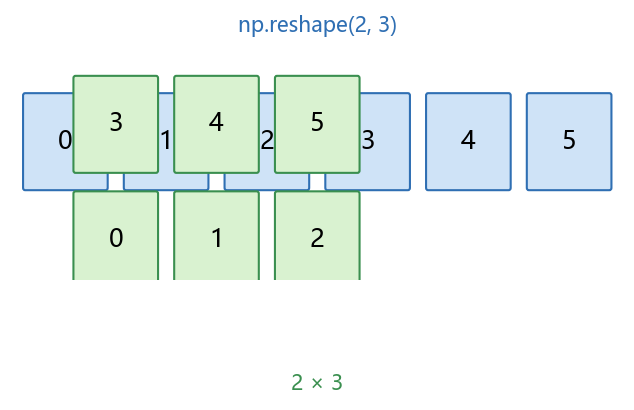
\includegraphics[keepaspectratio,alt={reshape 示意图}]{figures/01-numpy/reshape.png}}
\caption{reshape 示意图}
\end{figure}

\begin{itemize}
\tightlist
\item
  总元素数必须相等；
\item
  \texttt{reshape}
  在内存连续时通常返回\textbf{视图}（共享内存）；需要独立副本时用
  \texttt{arr.reshape(...).copy()}。
\end{itemize}

\subsubsection{1.3.2 展平：ravel vs
flatten}\label{ux5c55ux5e73ravel-vs-flatten}

\begin{Shaded}
\begin{Highlighting}[]
\NormalTok{a }\OperatorTok{=}\NormalTok{ np.array([[}\DecValTok{1}\NormalTok{, }\DecValTok{2}\NormalTok{, }\DecValTok{3}\NormalTok{], [}\DecValTok{4}\NormalTok{, }\DecValTok{5}\NormalTok{, }\DecValTok{6}\NormalTok{]])}
\NormalTok{a.ravel()    }\CommentTok{\# 视图（尽可能不拷贝）}
\NormalTok{a.flatten()  }\CommentTok{\# 总是拷贝}
\NormalTok{a.reshape(}\OperatorTok{{-}}\DecValTok{1}\NormalTok{)  }\CommentTok{\# 展平}
\end{Highlighting}
\end{Shaded}

\subsubsection{1.3.3 转置}\label{ux8f6cux7f6e}

\begin{Shaded}
\begin{Highlighting}[]
\NormalTok{a }\OperatorTok{=}\NormalTok{ np.arange(}\DecValTok{6}\NormalTok{).reshape(}\DecValTok{2}\NormalTok{, }\DecValTok{3}\NormalTok{)}
\NormalTok{a.T          }\CommentTok{\# 转置 (3,2)}
\NormalTok{np.transpose(a)            }\CommentTok{\# 等价}
\NormalTok{np.transpose(a, axes}\OperatorTok{=}\NormalTok{(}\DecValTok{1}\NormalTok{, }\DecValTok{0}\NormalTok{))  }\CommentTok{\# 高维时可指定轴的顺序}
\end{Highlighting}
\end{Shaded}

\subsubsection{1.3.4 拼接与堆叠}\label{ux62fcux63a5ux4e0eux5806ux53e0}

\begin{Shaded}
\begin{Highlighting}[]
\NormalTok{a }\OperatorTok{=}\NormalTok{ np.array([[}\DecValTok{1}\NormalTok{, }\DecValTok{2}\NormalTok{], [}\DecValTok{3}\NormalTok{, }\DecValTok{4}\NormalTok{]])}
\NormalTok{b }\OperatorTok{=}\NormalTok{ np.array([[}\DecValTok{5}\NormalTok{, }\DecValTok{6}\NormalTok{]])}
\NormalTok{np.concatenate((a, b), axis}\OperatorTok{=}\DecValTok{0}\NormalTok{)      }\CommentTok{\# 沿 0 轴拼接: (3,2)}
\NormalTok{np.concatenate((a, a), axis}\OperatorTok{=}\DecValTok{1}\NormalTok{)      }\CommentTok{\# 沿 1 轴拼接: (2,4)}
\NormalTok{np.vstack((a, b))                   }\CommentTok{\# 垂直堆叠}
\NormalTok{np.hstack((a, a))                   }\CommentTok{\# 水平堆叠}
\NormalTok{np.stack(([}\DecValTok{1}\NormalTok{, }\DecValTok{2}\NormalTok{], [}\DecValTok{3}\NormalTok{, }\DecValTok{4}\NormalTok{]), axis}\OperatorTok{=}\DecValTok{0}\NormalTok{)  }\CommentTok{\# 新增维度堆叠 (2,2)}
\NormalTok{np.column\_stack(([}\DecValTok{1}\NormalTok{, }\DecValTok{2}\NormalTok{], [}\DecValTok{3}\NormalTok{, }\DecValTok{4}\NormalTok{]))   }\CommentTok{\# 一维数组按列堆叠 (2,2)}
\end{Highlighting}
\end{Shaded}

\subsubsection{1.3.5 增删元素}\label{ux589eux5220ux5143ux7d20}

\begin{Shaded}
\begin{Highlighting}[]
\NormalTok{a }\OperatorTok{=}\NormalTok{ np.array([}\DecValTok{1}\NormalTok{, }\DecValTok{2}\NormalTok{, }\DecValTok{3}\NormalTok{])}
\NormalTok{np.append(a, }\DecValTok{4}\NormalTok{)              }\CommentTok{\# 返回新数组 [1 2 3 4]}
\NormalTok{np.delete(a, }\DecValTok{1}\NormalTok{)              }\CommentTok{\# 返回新数组 [1 3]}
\NormalTok{a[[}\DecValTok{0}\NormalTok{, }\DecValTok{2}\NormalTok{]]                    }\CommentTok{\# 花式索引取第 0、2 个}
\NormalTok{a[a }\OperatorTok{!=} \DecValTok{3}\NormalTok{]                    }\CommentTok{\# 布尔掩码过滤}
\end{Highlighting}
\end{Shaded}

\begin{quote}
频繁 \texttt{append}/\texttt{delete}
会反复拷贝，性能差；大数据请先想好形状或用列表收集。
\end{quote}

\begin{center}\rule{0.5\linewidth}{0.5pt}\end{center}

\subsection{1.4 索引与切片}\label{ux7d22ux5f15ux4e0eux5207ux7247}

\subsubsection{1.4.1
基本索引与切片（视图）}\label{ux57faux672cux7d22ux5f15ux4e0eux5207ux7247ux89c6ux56fe}

\begin{Shaded}
\begin{Highlighting}[]
\NormalTok{a }\OperatorTok{=}\NormalTok{ np.arange(}\DecValTok{10}\NormalTok{)}
\NormalTok{a[}\DecValTok{0}\NormalTok{]        }\CommentTok{\# 标量}
\NormalTok{a[}\DecValTok{2}\NormalTok{:}\DecValTok{5}\NormalTok{]      }\CommentTok{\# 视图，切片}
\NormalTok{a[::}\OperatorTok{{-}}\DecValTok{1}\NormalTok{]     }\CommentTok{\# 反转}
\end{Highlighting}
\end{Shaded}

二维数组：

\begin{Shaded}
\begin{Highlighting}[]
\NormalTok{m }\OperatorTok{=}\NormalTok{ np.arange(}\DecValTok{12}\NormalTok{).reshape(}\DecValTok{3}\NormalTok{, }\DecValTok{4}\NormalTok{)}
\NormalTok{m[}\DecValTok{0}\NormalTok{, }\DecValTok{1}\NormalTok{]      }\CommentTok{\# 第 0 行第 1 列}
\NormalTok{m[:, }\DecValTok{1}\NormalTok{]      }\CommentTok{\# 第 1 列（视图）}
\NormalTok{m[}\DecValTok{1}\NormalTok{:}\DecValTok{3}\NormalTok{, }\DecValTok{1}\NormalTok{:}\DecValTok{3}\NormalTok{]  }\CommentTok{\# 子矩阵（视图）}
\end{Highlighting}
\end{Shaded}

\subsubsection{1.4.2 花式索引（fancy
indexing，拷贝）}\label{ux82b1ux5f0fux7d22ux5f15fancy-indexingux62f7ux8d1d}

\begin{Shaded}
\begin{Highlighting}[]
\NormalTok{m }\OperatorTok{=}\NormalTok{ np.arange(}\DecValTok{12}\NormalTok{).reshape(}\DecValTok{3}\NormalTok{, }\DecValTok{4}\NormalTok{)}
\BuiltInTok{print}\NormalTok{(m[[}\DecValTok{0}\NormalTok{, }\DecValTok{2}\NormalTok{], [}\DecValTok{1}\NormalTok{, }\DecValTok{3}\NormalTok{]])     }\CommentTok{\# 取 (0,1) 和 (2,3) → [1 11]}
\BuiltInTok{print}\NormalTok{(m[np.ix\_([}\DecValTok{0}\NormalTok{, }\DecValTok{2}\NormalTok{], [}\DecValTok{1}\NormalTok{, }\DecValTok{3}\NormalTok{])])  }\CommentTok{\# 行×列交叉 → 2×2}
\end{Highlighting}
\end{Shaded}

\begin{Shaded}
\begin{Highlighting}[]
\NormalTok{[ 1 11]}
\NormalTok{[[ 1  3]}
\NormalTok{ [ 9 11]]}
\end{Highlighting}
\end{Shaded}

\subsubsection{1.4.3 布尔掩码}\label{ux5e03ux5c14ux63a9ux7801}

\begin{Shaded}
\begin{Highlighting}[]
\NormalTok{x }\OperatorTok{=}\NormalTok{ np.array([}\DecValTok{1}\NormalTok{, }\OperatorTok{{-}}\DecValTok{2}\NormalTok{, }\DecValTok{3}\NormalTok{, }\OperatorTok{{-}}\DecValTok{4}\NormalTok{, }\DecValTok{5}\NormalTok{])}
\NormalTok{mask }\OperatorTok{=}\NormalTok{ x }\OperatorTok{\textgreater{}} \DecValTok{0}
\BuiltInTok{print}\NormalTok{(mask)        }\CommentTok{\# [ True False  True False  True]}
\BuiltInTok{print}\NormalTok{(x[mask])     }\CommentTok{\# [1 3 5]}
\BuiltInTok{print}\NormalTok{(np.where(x }\OperatorTok{\textgreater{}} \DecValTok{0}\NormalTok{, x, }\DecValTok{0}\NormalTok{))   }\CommentTok{\# 正数保留，否则 0}
\end{Highlighting}
\end{Shaded}

\begin{quote}
布尔索引返回\textbf{拷贝}；条件组合用
\texttt{\&}、\texttt{\textbar{}}、\texttt{\textasciitilde{}}
且必须加括号，例如
\texttt{x{[}(x\ \textgreater{}\ 0)\ \&\ (x\ \textless{}\ 4){]}}。
\end{quote}

\begin{center}\rule{0.5\linewidth}{0.5pt}\end{center}

\subsection{1.5
视图与拷贝（重点）}\label{ux89c6ux56feux4e0eux62f7ux8d1dux91cdux70b9}

\begin{Shaded}
\begin{Highlighting}[]
\NormalTok{a }\OperatorTok{=}\NormalTok{ np.arange(}\DecValTok{6}\NormalTok{)}
\NormalTok{b }\OperatorTok{=}\NormalTok{ a.reshape(}\DecValTok{2}\NormalTok{, }\DecValTok{3}\NormalTok{)      }\CommentTok{\# 通常为视图}
\NormalTok{b[}\DecValTok{0}\NormalTok{, }\DecValTok{0}\NormalTok{] }\OperatorTok{=} \DecValTok{99}
\BuiltInTok{print}\NormalTok{(a[}\DecValTok{0}\NormalTok{])              }\CommentTok{\# 99 —— 共享内存！}

\NormalTok{c }\OperatorTok{=}\NormalTok{ a.copy()             }\CommentTok{\# 独立拷贝}
\NormalTok{c[}\DecValTok{0}\NormalTok{] }\OperatorTok{=} \OperatorTok{{-}}\DecValTok{1}
\BuiltInTok{print}\NormalTok{(a[}\DecValTok{0}\NormalTok{])              }\CommentTok{\# 仍为 99}

\BuiltInTok{print}\NormalTok{(a.base }\KeywordTok{is} \VariableTok{None}\NormalTok{)            }\CommentTok{\# 原始数组 base 为 None}
\BuiltInTok{print}\NormalTok{(b.base }\KeywordTok{is}\NormalTok{ a)               }\CommentTok{\# True → b 是 a 的视图}
\end{Highlighting}
\end{Shaded}

经验法则：

{\def\LTcaptype{none} % do not increment counter
\begin{longtable}[]{@{}ll@{}}
\toprule\noalign{}
操作 & 是否共享内存 \\
\midrule\noalign{}
\endhead
\bottomrule\noalign{}
\endlastfoot
基本切片 & 视图 \\
\texttt{reshape}（连续内存） & 视图（否则拷贝） \\
\texttt{ravel} & 视图（尽可能） \\
\texttt{flatten} & 拷贝 \\
花式索引 / 布尔索引 & 拷贝 \\
\texttt{copy()} & 拷贝 \\
\end{longtable}
}

\begin{center}\rule{0.5\linewidth}{0.5pt}\end{center}

\subsection{1.6
广播机制（broadcasting）}\label{ux5e7fux64adux673aux5236broadcasting}

\textbf{规则}：从最后一个维度往前比较
------（1）两维相等；（2）或其中一维为
1（可``拉伸''）；（3）或该维不存在（自动补 1）。都不满足则报错。

\begin{Shaded}
\begin{Highlighting}[]
\NormalTok{A }\OperatorTok{=}\NormalTok{ np.array([[}\DecValTok{1}\NormalTok{, }\DecValTok{2}\NormalTok{, }\DecValTok{3}\NormalTok{], [}\DecValTok{4}\NormalTok{, }\DecValTok{5}\NormalTok{, }\DecValTok{6}\NormalTok{]])   }\CommentTok{\# (2,3)}
\NormalTok{b }\OperatorTok{=}\NormalTok{ np.array([}\DecValTok{10}\NormalTok{, }\DecValTok{20}\NormalTok{, }\DecValTok{30}\NormalTok{])             }\CommentTok{\# (3,) → 看作 (1,3)}
\BuiltInTok{print}\NormalTok{(A }\OperatorTok{+}\NormalTok{ b)}
\end{Highlighting}
\end{Shaded}

\begin{Shaded}
\begin{Highlighting}[]
\NormalTok{[[11 22 33]}
\NormalTok{ [14 25 36]]}
\end{Highlighting}
\end{Shaded}

\begin{figure}
\centering
\pandocbounded{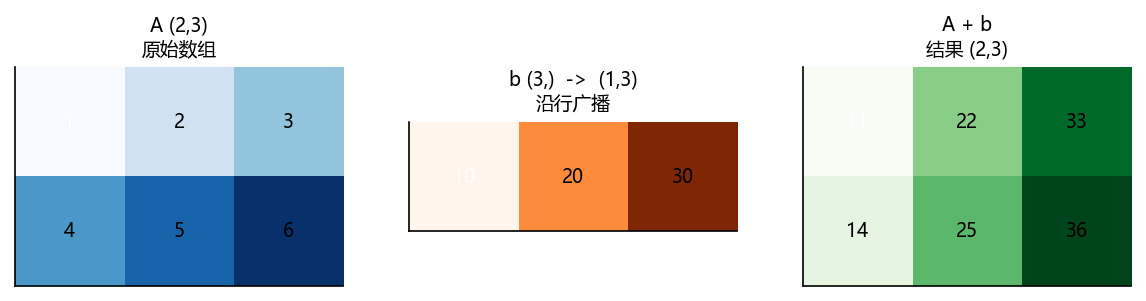
\includegraphics[keepaspectratio,alt={广播示意图}]{figures/01-numpy/broadcast.png}}
\caption{广播示意图}
\end{figure}

\begin{itemize}
\tightlist
\item
  \texttt{(2,3)\ +\ (3,)} √，结果为 \texttt{(2,3)}；
\item
  \texttt{(3,)\ +\ (4,)} ×（末尾不等且无 1）；
\item
  \texttt{(4,1)\ +\ (1,3)} √，结果 \texttt{(4,3)}；
\item
  \texttt{(4,1,6)\ +\ (3,6)} √，结果 \texttt{(4,3,6)}（把 \texttt{(3,6)}
  补成 \texttt{(1,3,6)}）。
\end{itemize}

\textbf{调试技巧}：报错时打印两个数组的 \texttt{shape}，用
\texttt{np.newaxis}（即 \texttt{None}）手动补维。

\begin{center}\rule{0.5\linewidth}{0.5pt}\end{center}

\subsection{1.7
随机数生成与抽样}\label{ux968fux673aux6570ux751fux6210ux4e0eux62bdux6837}

\subsubsection{1.7.1
新版推荐：Generator}\label{ux65b0ux7248ux63a8ux8350generator}

\begin{Shaded}
\begin{Highlighting}[]
\NormalTok{rng }\OperatorTok{=}\NormalTok{ np.random.default\_rng(}\DecValTok{42}\NormalTok{)      }\CommentTok{\# 固定种子，结果可复现}
\NormalTok{rng.random((}\DecValTok{2}\NormalTok{, }\DecValTok{3}\NormalTok{))                   }\CommentTok{\# [0,1) 均匀}
\NormalTok{rng.integers(}\DecValTok{1}\NormalTok{, }\DecValTok{10}\NormalTok{, size}\OperatorTok{=}\DecValTok{5}\NormalTok{)          }\CommentTok{\# 整数 [1,10)}
\NormalTok{rng.uniform(}\OperatorTok{{-}}\DecValTok{1}\NormalTok{, }\DecValTok{1}\NormalTok{, size}\OperatorTok{=}\DecValTok{4}\NormalTok{)           }\CommentTok{\# 均匀分布}
\NormalTok{rng.normal(}\DecValTok{2}\NormalTok{, }\FloatTok{0.5}\NormalTok{, size}\OperatorTok{=}\DecValTok{6}\NormalTok{)           }\CommentTok{\# 正态 N(2, 0.5\^{}2)}
\end{Highlighting}
\end{Shaded}

\subsubsection{1.7.2
旧接口（仍可用，但不建议用于新代码）}\label{ux65e7ux63a5ux53e3ux4ecdux53efux7528ux4f46ux4e0dux5efaux8baeux7528ux4e8eux65b0ux4ee3ux7801}

\begin{Shaded}
\begin{Highlighting}[]
\NormalTok{np.random.seed(}\DecValTok{42}\NormalTok{)}
\NormalTok{np.random.rand(}\DecValTok{2}\NormalTok{, }\DecValTok{3}\NormalTok{)     }\CommentTok{\# [0,1)}
\NormalTok{np.random.randint(}\DecValTok{1}\NormalTok{, }\DecValTok{10}\NormalTok{) }\CommentTok{\# 整数}
\NormalTok{np.random.randn(}\DecValTok{5}\NormalTok{)       }\CommentTok{\# 标准正态}
\NormalTok{np.random.normal(}\DecValTok{2}\NormalTok{, }\FloatTok{0.5}\NormalTok{, }\DecValTok{5}\NormalTok{)}
\end{Highlighting}
\end{Shaded}

\textbf{选型}：新代码优先
\texttt{default\_rng}（更快、线程安全、接口清晰）。

\begin{center}\rule{0.5\linewidth}{0.5pt}\end{center}

\subsection{常见误区}\label{ux5e38ux89c1ux8befux533a}

\begin{enumerate}
\def\labelenumi{\arabic{enumi}.}
\tightlist
\item
  \textbf{\texttt{*} 不等于矩阵乘法}：\texttt{A\ *\ B}
  是逐元素乘法；矩阵乘法用 \texttt{A\ @\ B} 或 \texttt{np.matmul}。
\item
  \textbf{忘记 \texttt{zeros/ones/full}
  要传元组}：\texttt{np.zeros(2,\ 3)} 会报错，应为
  \texttt{np.zeros((2,\ 3))}。
\item
  \textbf{以为 \texttt{reshape}
  一定返回拷贝}：连续内存下是视图；改视图会影响原数组。
\item
  \textbf{误用
  \texttt{len(a)}}：一维数组返回长度，二维返回行数；看形状用
  \texttt{a.shape}。
\item
  \textbf{广播不通用}：\texttt{(3,)\ +\ (4,)} 不会自动``截断对齐''。
\item
  \textbf{随机数不设种子}：不设种子结果每次不同，课堂演示/作业请用
  \texttt{default\_rng(seed)}。
\end{enumerate}

\subsection{思考题}\label{ux601dux8003ux9898}

\begin{enumerate}
\def\labelenumi{\arabic{enumi}.}
\tightlist
\item
  \texttt{np.arange(10){[}::2{]}} 与
  \texttt{np.arange(10).reshape(5,2){[}:,0{]}} 是否共享内存？用
  `\texttt{.base} 验证。
\item
  解释 \texttt{np.ix\_} 与同时传入两个顺序索引的区别。
\item
  举一个形状满足广播规则却``符合直觉但结果错误''的例子（提示：\texttt{(3,1)}
  与 \texttt{(3,)}）。
\end{enumerate}

\subsection{动手练习（详见
lab）}\label{ux52a8ux624bux7ec3ux4e60ux8be6ux89c1-lab}

\begin{itemize}
\tightlist
\item
  创建 3×4 矩阵，用布尔掩码把负数置 0；
\item
  用 \texttt{np.arange} 生成 0--100 的偶数，转成 10×5 矩阵；
\item
  复现``对每列做不同缩放''的广播例子；
\item
  用 \texttt{default\_rng(0)} 生成 100 个标准正态数并统计均值/方差。
\end{itemize}

\subsection{延伸阅读}\label{ux5ef6ux4f38ux9605ux8bfb}

\begin{itemize}
\tightlist
\item
  NumPy
  官方绝对入门：https://numpy.org/doc/stable/user/absolute\_beginners.html
\item
  NumPy
  官方广播机制：https://numpy.org/doc/stable/user/basics.broadcasting.html
\item
  SciPy Lecture Notes --
  NumPy：https://scipy-lectures.org/intro/numpy/index.html
\end{itemize}

\section{02
数组运算：向量、矩阵、逻辑筛选与统计}\label{ux6570ux7ec4ux8fd0ux7b97ux5411ux91cfux77e9ux9635ux903bux8f91ux7b5bux9009ux4e0eux7edfux8ba1}

\begin{quote}
本节对应原版 1.2 的内容，并增补学习目标、常见误区、思考题与延伸阅读。
配套图：\texttt{figures/01-numpy/vector\_ops.png}。
\end{quote}

\subsection{本节目标}\label{ux672cux8282ux76eeux6807-1}

\begin{itemize}
\tightlist
\item
  区分\textbf{逐元素运算}与\textbf{线性代数运算}（\texttt{*} vs
  \texttt{@} / \texttt{dot}）；
\item
  会用布尔掩码与 \texttt{np.where} 做筛选与替换；
\item
  掌握 \texttt{sum/mean/std/min/max} 沿 \texttt{axis} 方向统计；
\item
  会用 \texttt{sort/argsort} 排序与排名；
\item
  会用
  \texttt{savetxt/loadtxt}、\texttt{save/load}、\texttt{savez\_compressed}
  保存与读取数组。
\end{itemize}

\subsection{先修}\label{ux5148ux4fee-1}

\begin{itemize}
\tightlist
\item
  01 数组基础（创建、索引、广播）。
\end{itemize}

\begin{center}\rule{0.5\linewidth}{0.5pt}\end{center}

\subsection{2.1 向量的运算}\label{ux5411ux91cfux7684ux8fd0ux7b97}

\subsubsection{2.1.1 逐元素操作}\label{ux9010ux5143ux7d20ux64cdux4f5c}

\begin{Shaded}
\begin{Highlighting}[]
\ImportTok{import}\NormalTok{ numpy }\ImportTok{as}\NormalTok{ np}

\NormalTok{v }\OperatorTok{=}\NormalTok{ np.array([}\DecValTok{2}\NormalTok{, }\DecValTok{3}\NormalTok{])}
\NormalTok{w }\OperatorTok{=}\NormalTok{ np.array([}\DecValTok{3}\NormalTok{, }\DecValTok{1}\NormalTok{])}
\BuiltInTok{print}\NormalTok{(v }\OperatorTok{+}\NormalTok{ w)     }\CommentTok{\# [5 4]}
\BuiltInTok{print}\NormalTok{(v }\OperatorTok{{-}}\NormalTok{ w)     }\CommentTok{\# [{-}1  2]}
\BuiltInTok{print}\NormalTok{(}\DecValTok{2} \OperatorTok{*}\NormalTok{ v)     }\CommentTok{\# [4 6]}
\BuiltInTok{print}\NormalTok{(v }\OperatorTok{*}\NormalTok{ w)     }\CommentTok{\# 逐元素乘 [6 3]}
\BuiltInTok{print}\NormalTok{(v }\OperatorTok{/}\NormalTok{ w)     }\CommentTok{\# 逐元素除 [0.66666667 3.        ]}
\BuiltInTok{print}\NormalTok{(v }\OperatorTok{**} \DecValTok{2}\NormalTok{)    }\CommentTok{\# 逐元素平方 [4 9]}
\end{Highlighting}
\end{Shaded}

\begin{figure}
\centering
\pandocbounded{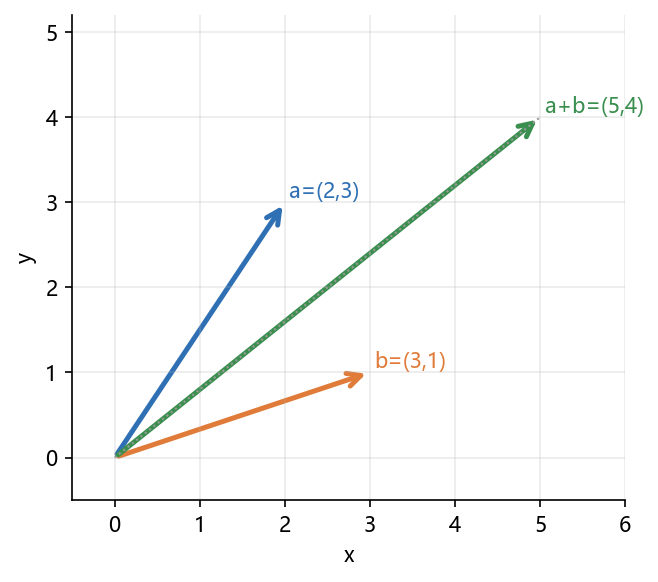
\includegraphics[keepaspectratio,alt={向量运算示意}]{figures/01-numpy/vector_ops.png}}
\caption{向量运算示意}
\end{figure}

\subsubsection{2.1.2
数量积（点积）与叉积}\label{ux6570ux91cfux79efux70b9ux79efux4e0eux53c9ux79ef}

\begin{Shaded}
\begin{Highlighting}[]
\NormalTok{a }\OperatorTok{=}\NormalTok{ np.array([}\DecValTok{1}\NormalTok{, }\DecValTok{2}\NormalTok{])}
\NormalTok{b }\OperatorTok{=}\NormalTok{ np.array([}\DecValTok{3}\NormalTok{, }\DecValTok{4}\NormalTok{])}
\BuiltInTok{print}\NormalTok{(np.dot(a, b))      }\CommentTok{\# 1*3 + 2*4 = 11}
\BuiltInTok{print}\NormalTok{(a }\OperatorTok{@}\NormalTok{ b)             }\CommentTok{\# 向量点积同样可用 @}

\NormalTok{c }\OperatorTok{=}\NormalTok{ np.array([}\DecValTok{1}\NormalTok{, }\DecValTok{2}\NormalTok{, }\DecValTok{3}\NormalTok{])}
\NormalTok{d }\OperatorTok{=}\NormalTok{ np.array([}\DecValTok{4}\NormalTok{, }\DecValTok{5}\NormalTok{, }\DecValTok{6}\NormalTok{])}
\BuiltInTok{print}\NormalTok{(np.cross(c, d))    }\CommentTok{\# [{-}3  6 {-}3]}
\end{Highlighting}
\end{Shaded}

\subsubsection{2.1.3 向量的范数}\label{ux5411ux91cfux7684ux8303ux6570}

\begin{Shaded}
\begin{Highlighting}[]
\NormalTok{x }\OperatorTok{=}\NormalTok{ np.array([}\DecValTok{3}\NormalTok{, }\DecValTok{4}\NormalTok{])}
\NormalTok{np.linalg.norm(x)        }\CommentTok{\# 5.0（默认 2{-}范数）}
\NormalTok{np.linalg.norm(x, }\BuiltInTok{ord}\OperatorTok{=}\DecValTok{1}\NormalTok{) }\CommentTok{\# 7.0（1{-}范数）}
\end{Highlighting}
\end{Shaded}

\subsubsection{2.1.4 排序}\label{ux6392ux5e8f}

\begin{Shaded}
\begin{Highlighting}[]
\NormalTok{a }\OperatorTok{=}\NormalTok{ np.array([}\DecValTok{3}\NormalTok{, }\DecValTok{1}\NormalTok{, }\DecValTok{2}\NormalTok{])}
\NormalTok{np.sort(a)          }\CommentTok{\# 返回新数组 [1 2 3]}
\NormalTok{a.sort()            }\CommentTok{\# 原地排序}
\NormalTok{np.argsort(a)       }\CommentTok{\# 排序后原索引}
\end{Highlighting}
\end{Shaded}

\begin{center}\rule{0.5\linewidth}{0.5pt}\end{center}

\subsection{2.2
向量/矩阵的逻辑运算------筛选}\label{ux5411ux91cfux77e9ux9635ux7684ux903bux8f91ux8fd0ux7b97ux7b5bux9009}

\begin{Shaded}
\begin{Highlighting}[]
\NormalTok{x }\OperatorTok{=}\NormalTok{ np.array([}\DecValTok{1}\NormalTok{, }\OperatorTok{{-}}\DecValTok{2}\NormalTok{, }\DecValTok{3}\NormalTok{, }\OperatorTok{{-}}\DecValTok{4}\NormalTok{, }\DecValTok{5}\NormalTok{])}

\CommentTok{\#\# 布尔掩码}
\BuiltInTok{print}\NormalTok{(x[x }\OperatorTok{\textgreater{}} \DecValTok{0}\NormalTok{])          }\CommentTok{\# [1 3 5]}
\BuiltInTok{print}\NormalTok{(x[(x }\OperatorTok{\textgreater{}} \DecValTok{1}\NormalTok{) }\OperatorTok{\&}\NormalTok{ (x }\OperatorTok{\textless{}} \DecValTok{5}\NormalTok{)])  }\CommentTok{\# [3]}

\CommentTok{\#\# np.where：条件成立取第一项，否则取第二项}
\BuiltInTok{print}\NormalTok{(np.where(x }\OperatorTok{\textgreater{}} \DecValTok{0}\NormalTok{, x, }\DecValTok{0}\NormalTok{))   }\CommentTok{\# [1 0 3 0 5]}
\end{Highlighting}
\end{Shaded}

二维按行筛选：

\begin{Shaded}
\begin{Highlighting}[]
\NormalTok{m }\OperatorTok{=}\NormalTok{ np.array([[}\DecValTok{1}\NormalTok{, }\DecValTok{9}\NormalTok{], [}\DecValTok{6}\NormalTok{, }\DecValTok{2}\NormalTok{], [}\DecValTok{7}\NormalTok{, }\DecValTok{8}\NormalTok{]])}
\BuiltInTok{print}\NormalTok{(m[(m[:, }\DecValTok{0}\NormalTok{] }\OperatorTok{\textgreater{}} \DecValTok{3}\NormalTok{) }\OperatorTok{\&}\NormalTok{ (m[:, }\DecValTok{1}\NormalTok{] }\OperatorTok{\textless{}} \DecValTok{9}\NormalTok{)])   }\CommentTok{\# [[6 2] [7 8]]}
\end{Highlighting}
\end{Shaded}

\begin{quote}
组合条件必须加括号，且不能用 \texttt{and} / \texttt{or}，要用
\texttt{\&} / \texttt{\textbar{}} / \texttt{\textasciitilde{}}。
\end{quote}

\begin{center}\rule{0.5\linewidth}{0.5pt}\end{center}

\subsection{2.3 矩阵的运算}\label{ux77e9ux9635ux7684ux8fd0ux7b97}

\subsubsection{2.3.1 算术运算}\label{ux7b97ux672fux8fd0ux7b97}

\begin{Shaded}
\begin{Highlighting}[]
\NormalTok{A }\OperatorTok{=}\NormalTok{ np.array([[}\DecValTok{1}\NormalTok{, }\DecValTok{2}\NormalTok{], [}\DecValTok{3}\NormalTok{, }\DecValTok{4}\NormalTok{]])}
\NormalTok{B }\OperatorTok{=}\NormalTok{ np.array([[}\DecValTok{5}\NormalTok{, }\DecValTok{6}\NormalTok{], [}\DecValTok{7}\NormalTok{, }\DecValTok{8}\NormalTok{]])}

\BuiltInTok{print}\NormalTok{(A }\OperatorTok{+}\NormalTok{ B)      }\CommentTok{\# 矩阵加法 [[ 6  8][10 12]]}
\BuiltInTok{print}\NormalTok{(A }\OperatorTok{{-}}\NormalTok{ B)      }\CommentTok{\# 矩阵减法}
\BuiltInTok{print}\NormalTok{(A }\OperatorTok{*}\NormalTok{ B)      }\CommentTok{\# 注意：逐元素乘 [[ 5 12][21 32]]}
\BuiltInTok{print}\NormalTok{(A }\OperatorTok{@}\NormalTok{ B)      }\CommentTok{\# √ 矩阵乘 [[19 22][43 50]]}
\BuiltInTok{print}\NormalTok{(np.matmul(A, B))   }\CommentTok{\# 同 @}
\end{Highlighting}
\end{Shaded}

\textbf{为什么 \texttt{*} 不是矩阵乘}：NumPy 中 \texttt{*} 是
\texttt{ufunc} 的逐元素运算；要数学上的矩阵乘法，用 \texttt{@}（或
\texttt{np.dot} / \texttt{np.matmul}，二者在 2D 下等价，但 \texttt{@}
语义更明确）。

\subsubsection{2.3.2
矩阵上的统计}\label{ux77e9ux9635ux4e0aux7684ux7edfux8ba1}

\begin{Shaded}
\begin{Highlighting}[]
\NormalTok{S }\OperatorTok{=}\NormalTok{ np.array([[}\DecValTok{85}\NormalTok{, }\DecValTok{90}\NormalTok{, }\DecValTok{80}\NormalTok{],}
\NormalTok{              [}\DecValTok{78}\NormalTok{, }\DecValTok{85}\NormalTok{, }\DecValTok{90}\NormalTok{],}
\NormalTok{              [}\DecValTok{90}\NormalTok{, }\DecValTok{95}\NormalTok{, }\DecValTok{85}\NormalTok{]])}

\NormalTok{S.}\BuiltInTok{sum}\NormalTok{(axis}\OperatorTok{=}\DecValTok{0}\NormalTok{)      }\CommentTok{\# 每列和 [253 270 255]（三门课总分）}
\NormalTok{S.}\BuiltInTok{sum}\NormalTok{(axis}\OperatorTok{=}\DecValTok{1}\NormalTok{)      }\CommentTok{\# 每行和 [255 253 270]（每个学生总分）}
\NormalTok{S.mean(axis}\OperatorTok{=}\DecValTok{0}\NormalTok{)     }\CommentTok{\# 每列均值 [84.33 90. 85. ]}
\NormalTok{S.}\BuiltInTok{max}\NormalTok{(axis}\OperatorTok{=}\DecValTok{1}\NormalTok{)      }\CommentTok{\# 每行最大值}
\NormalTok{S.std()            }\CommentTok{\# 全体标准差}
\end{Highlighting}
\end{Shaded}

记忆：\texttt{axis=0} 表示``沿第 0
轴（行方向）折叠''，即求\textbf{每列}的统计量；\texttt{axis=1}
求\textbf{每行}。

\subsubsection{2.3.3 查找（where /
argmax）}\label{ux67e5ux627ewhere-argmax}

\begin{Shaded}
\begin{Highlighting}[]
\NormalTok{m }\OperatorTok{=}\NormalTok{ np.array([[}\DecValTok{3}\NormalTok{, }\DecValTok{7}\NormalTok{], [}\DecValTok{9}\NormalTok{, }\DecValTok{2}\NormalTok{]])}
\NormalTok{np.where(m }\OperatorTok{\textgreater{}} \DecValTok{5}\NormalTok{)          }\CommentTok{\# (array([0,1]), array([1,0])) 坐标}
\NormalTok{np.argmax(m)             }\CommentTok{\# 展平后的最大索引 2 → (1,0)}
\NormalTok{np.argmax(m, axis}\OperatorTok{=}\DecValTok{1}\NormalTok{)     }\CommentTok{\# 每行最大索引 [1 0]}
\end{Highlighting}
\end{Shaded}

\begin{center}\rule{0.5\linewidth}{0.5pt}\end{center}

\subsection{2.4
结果的保存与读取}\label{ux7ed3ux679cux7684ux4fddux5b58ux4e0eux8bfbux53d6}

\begin{Shaded}
\begin{Highlighting}[]
\NormalTok{a }\OperatorTok{=}\NormalTok{ np.array([[}\DecValTok{1}\NormalTok{, }\DecValTok{2}\NormalTok{], [}\DecValTok{3}\NormalTok{, }\DecValTok{4}\NormalTok{]])}

\CommentTok{\#\# 文本}
\NormalTok{np.savetxt(}\StringTok{"result.txt"}\NormalTok{, a, fmt}\OperatorTok{=}\StringTok{"}\SpecialCharTok{\%.2f}\StringTok{"}\NormalTok{, delimiter}\OperatorTok{=}\StringTok{","}\NormalTok{)}
\NormalTok{b }\OperatorTok{=}\NormalTok{ np.loadtxt(}\StringTok{"result.txt"}\NormalTok{, delimiter}\OperatorTok{=}\StringTok{","}\NormalTok{)}

\CommentTok{\#\# 二进制（推荐：更快、保留 dtype）}
\NormalTok{np.save(}\StringTok{"a.npy"}\NormalTok{, a)}
\NormalTok{c }\OperatorTok{=}\NormalTok{ np.load(}\StringTok{"a.npy"}\NormalTok{)}

\CommentTok{\#\# 多数组压缩保存}
\NormalTok{np.savez\_compressed(}\StringTok{"data.npz"}\NormalTok{, x}\OperatorTok{=}\NormalTok{a, y}\OperatorTok{=}\NormalTok{b)}
\NormalTok{d }\OperatorTok{=}\NormalTok{ np.load(}\StringTok{"data.npz"}\NormalTok{)}
\NormalTok{d[}\StringTok{"x"}\NormalTok{], d[}\StringTok{"y"}\NormalTok{]}
\end{Highlighting}
\end{Shaded}

\begin{center}\rule{0.5\linewidth}{0.5pt}\end{center}

\subsection{常见误区}\label{ux5e38ux89c1ux8befux533a-1}

\begin{enumerate}
\def\labelenumi{\arabic{enumi}.}
\tightlist
\item
  \textbf{\texttt{*} 与 \texttt{@} 混用}：\texttt{A\ *\ B}
  是逐元素乘；数学矩阵乘必须 \texttt{@}。
\item
  \textbf{axis 方向记反}：\texttt{sum(axis=0)} 是``消除第 0
  维''，得到每列结果。
\item
  \textbf{条件用 \texttt{and}/\texttt{or}}：数组布尔运算必须
  \texttt{\&}/\texttt{\textbar{}}，且每个条件加括号。
\item
  \textbf{反复
  \texttt{np.append}}：每次产生新数组，大数组循环中极慢；先估算容量或用列表。
\item
  \textbf{\texttt{np.dot} 语义在多维下容易混淆}：明确用 \texttt{@}
  更直观。
\end{enumerate}

\subsection{思考题}\label{ux601dux8003ux9898-1}

\begin{enumerate}
\def\labelenumi{\arabic{enumi}.}
\tightlist
\item
  \texttt{np.dot}、\texttt{np.matmul}、\texttt{@}
  在三维数组上行为是否一致？查文档说明。
\item
  为什么 \texttt{np.where(cond,\ x,\ y)} 要求 \texttt{x}、\texttt{y}
  可广播到 \texttt{cond} 的形状？
\item
  用 \texttt{argsort} 给三位学生按总分排名。
\end{enumerate}

\subsection{动手练习（详见
lab）}\label{ux52a8ux624bux7ec3ux4e60ux8be6ux89c1-lab-1}

\begin{itemize}
\tightlist
\item
  生成 5×5 随机矩阵，把主对角线元素置 0；
\item
  对每列做 z-score 标准化（\texttt{(x\ -\ mean)\ /\ std}），并比较
  \texttt{axis} 的选择；
\item
  用 \texttt{savetxt}/\texttt{loadtxt} 存取一份成绩表并检查数值一致。
\end{itemize}

\subsection{延伸阅读}\label{ux5ef6ux4f38ux9605ux8bfb-1}

\begin{itemize}
\tightlist
\item
  NumPy 官方 ndarray
  基础：https://numpy.org/doc/stable/user/quickstart.html
\item
  NumPy 官方 I/O
  说明：https://numpy.org/doc/stable/reference/routines.io.html
\item
  SciPy Lecture Notes --
  数组操作：https://scipy-lectures.org/intro/numpy/operations.html
\end{itemize}

\section{03 线性代数：逆、方程组、分解与
SVD}\label{ux7ebfux6027ux4ee3ux6570ux9006ux65b9ux7a0bux7ec4ux5206ux89e3ux4e0e-svd}

\begin{quote}
本节对应原版 1.3 的内容，并增补学习目标、常见误区、思考题与延伸阅读。
配套图：\texttt{figures/01-numpy/cond\_sensitivity.png}、\texttt{figures/01-numpy/svd\_compression.png}。
\end{quote}

\subsection{本节目标}\label{ux672cux8282ux76eeux6807-2}

\begin{itemize}
\tightlist
\item
  会求逆矩阵、伪逆、秩、行列式、范数；
\item
  会用 \texttt{np.linalg.solve} 解线性方程组，理解条件数（condition
  number）对数值稳定的影响；
\item
  会用 \texttt{np.linalg.lstsq} 做最小二乘；
\item
  掌握特征值分解、SVD、Cholesky、QR 分解的基本用法与适用场景；
\item
  能说出 SVD 的``压缩/降维''思想（见 05 综合案例）。
\end{itemize}

\subsection{先修}\label{ux5148ux4fee-2}

\begin{itemize}
\tightlist
\item
  01 数组基础、02 数组运算；线性代数的基本概念（矩阵、行列式、特征值）。
\end{itemize}

\begin{center}\rule{0.5\linewidth}{0.5pt}\end{center}

\subsection{3.1
基本线性代数运算}\label{ux57faux672cux7ebfux6027ux4ee3ux6570ux8fd0ux7b97}

\subsubsection{3.1.1
逆矩阵与伪逆}\label{ux9006ux77e9ux9635ux4e0eux4f2aux9006}

\begin{Shaded}
\begin{Highlighting}[]
\ImportTok{import}\NormalTok{ numpy }\ImportTok{as}\NormalTok{ np}

\NormalTok{A }\OperatorTok{=}\NormalTok{ np.array([[}\DecValTok{3}\NormalTok{, }\DecValTok{1}\NormalTok{], [}\DecValTok{1}\NormalTok{, }\DecValTok{2}\NormalTok{]])}
\NormalTok{A\_inv }\OperatorTok{=}\NormalTok{ np.linalg.inv(A)}
\BuiltInTok{print}\NormalTok{(A\_inv)}
\CommentTok{\#\# [[ 0.4 {-}0.2]}
\CommentTok{\#\#  [{-}0.2  0.6]]}
\BuiltInTok{print}\NormalTok{(A }\OperatorTok{@}\NormalTok{ A\_inv)      }\CommentTok{\# ≈ 单位矩阵}
\end{Highlighting}
\end{Shaded}

非方阵或奇异矩阵用 \texttt{pinv}（伪逆），常用于最小二乘与超定方程组：

\begin{Shaded}
\begin{Highlighting}[]
\NormalTok{B }\OperatorTok{=}\NormalTok{ np.array([[}\DecValTok{1}\NormalTok{, }\DecValTok{2}\NormalTok{], [}\DecValTok{2}\NormalTok{, }\DecValTok{4}\NormalTok{], [}\DecValTok{3}\NormalTok{, }\DecValTok{6}\NormalTok{]])   }\CommentTok{\# 秩亏}
\BuiltInTok{print}\NormalTok{(np.linalg.pinv(B).shape)           }\CommentTok{\# (2,3)}
\end{Highlighting}
\end{Shaded}

\subsubsection{3.1.2 秩}\label{ux79e9}

\begin{Shaded}
\begin{Highlighting}[]
\NormalTok{np.linalg.matrix\_rank(np.array([[}\DecValTok{1}\NormalTok{, }\DecValTok{2}\NormalTok{], [}\DecValTok{2}\NormalTok{, }\DecValTok{4}\NormalTok{]]))   }\CommentTok{\# 1（第二行是第一行的 2 倍）}
\NormalTok{np.linalg.matrix\_rank(np.array([[}\DecValTok{1}\NormalTok{, }\DecValTok{2}\NormalTok{], [}\DecValTok{3}\NormalTok{, }\DecValTok{4}\NormalTok{]]))   }\CommentTok{\# 2}
\end{Highlighting}
\end{Shaded}

\subsubsection{3.1.3 行列式}\label{ux884cux5217ux5f0f}

\begin{Shaded}
\begin{Highlighting}[]
\NormalTok{A }\OperatorTok{=}\NormalTok{ np.array([[}\DecValTok{3}\NormalTok{, }\DecValTok{1}\NormalTok{], [}\DecValTok{1}\NormalTok{, }\DecValTok{2}\NormalTok{]])}
\BuiltInTok{print}\NormalTok{(np.linalg.det(A))    }\CommentTok{\# 5.0（近似）}
\end{Highlighting}
\end{Shaded}

行列式为 0 等价于矩阵奇异，此时方程组没有唯一解。

\subsubsection{3.1.4 范数}\label{ux8303ux6570}

\begin{Shaded}
\begin{Highlighting}[]
\NormalTok{v }\OperatorTok{=}\NormalTok{ np.array([}\DecValTok{3}\NormalTok{, }\DecValTok{4}\NormalTok{])}
\NormalTok{np.linalg.norm(v)              }\CommentTok{\# 5.0，2{-}范数}
\NormalTok{np.linalg.norm(v, }\BuiltInTok{ord}\OperatorTok{=}\DecValTok{1}\NormalTok{)       }\CommentTok{\# 7.0}

\NormalTok{M }\OperatorTok{=}\NormalTok{ np.array([[}\DecValTok{3}\NormalTok{, }\DecValTok{4}\NormalTok{], [}\DecValTok{0}\NormalTok{, }\DecValTok{5}\NormalTok{]])}
\NormalTok{np.linalg.norm(M)              }\CommentTok{\# Frobenius 范数 ≈ 7.0711}
\NormalTok{np.linalg.norm(M, }\BuiltInTok{ord}\OperatorTok{=}\DecValTok{2}\NormalTok{)       }\CommentTok{\# 谱范数（最大奇异值）}
\NormalTok{np.linalg.norm(M, }\BuiltInTok{ord}\OperatorTok{=}\NormalTok{np.inf)  }\CommentTok{\# 无穷范数（行和最大值）}
\end{Highlighting}
\end{Shaded}

\begin{center}\rule{0.5\linewidth}{0.5pt}\end{center}

\subsection{3.2
线性方程组的求解}\label{ux7ebfux6027ux65b9ux7a0bux7ec4ux7684ux6c42ux89e3}

\subsubsection{\texorpdfstring{3.2.1
直接求解：\texttt{np.linalg.solve}}{3.2.1 直接求解：np.linalg.solve}}\label{ux76f4ux63a5ux6c42ux89e3np.linalg.solve}

\begin{Shaded}
\begin{Highlighting}[]
\NormalTok{A }\OperatorTok{=}\NormalTok{ np.array([[}\DecValTok{3}\NormalTok{, }\DecValTok{1}\NormalTok{], [}\DecValTok{1}\NormalTok{, }\DecValTok{2}\NormalTok{]])   }\CommentTok{\# 系数矩阵}
\NormalTok{b }\OperatorTok{=}\NormalTok{ np.array([}\DecValTok{9}\NormalTok{, }\DecValTok{8}\NormalTok{])             }\CommentTok{\# 常数向量}
\NormalTok{x }\OperatorTok{=}\NormalTok{ np.linalg.solve(A, b)}
\BuiltInTok{print}\NormalTok{(x)          }\CommentTok{\# [2. 3.]，即 x=2, y=3}
\BuiltInTok{print}\NormalTok{(A }\OperatorTok{@}\NormalTok{ x)      }\CommentTok{\# ≈ [9. 8.]}
\end{Highlighting}
\end{Shaded}

\textbf{适用条件}：\texttt{A}
是方阵且非奇异（存在唯一解）。结构更一般的线性方程组用 \texttt{lstsq}。

\subsubsection{\texorpdfstring{3.2.2
最小二乘：\texttt{np.linalg.lstsq}}{3.2.2 最小二乘：np.linalg.lstsq}}\label{ux6700ux5c0fux4e8cux4e58np.linalg.lstsq}

超定（方程多于未知数）或欠定（方程少于未知数）时，求``误差平方和最小''的解：

\begin{Shaded}
\begin{Highlighting}[]
\NormalTok{X }\OperatorTok{=}\NormalTok{ np.array([[}\DecValTok{1}\NormalTok{, }\DecValTok{1}\NormalTok{], [}\DecValTok{1}\NormalTok{, }\DecValTok{2}\NormalTok{], [}\DecValTok{1}\NormalTok{, }\DecValTok{3}\NormalTok{], [}\DecValTok{1}\NormalTok{, }\DecValTok{4}\NormalTok{]])}
\NormalTok{y }\OperatorTok{=}\NormalTok{ np.array([}\DecValTok{6}\NormalTok{, }\DecValTok{5}\NormalTok{, }\DecValTok{7}\NormalTok{, }\DecValTok{10}\NormalTok{])}
\NormalTok{coef, residuals, rank, sv }\OperatorTok{=}\NormalTok{ np.linalg.lstsq(X, y, rcond}\OperatorTok{=}\VariableTok{None}\NormalTok{)}
\BuiltInTok{print}\NormalTok{(coef)      }\CommentTok{\# [3.5 1.4] → y ≈ 3.5 + 1.4 x}
\end{Highlighting}
\end{Shaded}

\subsubsection{3.2.3
条件数与数值稳定性}\label{ux6761ux4ef6ux6570ux4e0eux6570ux503cux7a33ux5b9aux6027}

条件数 \texttt{cond(A)}
刻画方程组对扰动的敏感程度：条件数越大，解越``脆弱''。

\begin{Shaded}
\begin{Highlighting}[]
\NormalTok{A }\OperatorTok{=}\NormalTok{ np.array([[}\DecValTok{1}\NormalTok{, }\DecValTok{2}\NormalTok{, }\DecValTok{3}\NormalTok{],}
\NormalTok{              [}\DecValTok{2}\NormalTok{, }\FloatTok{4.0001}\NormalTok{, }\DecValTok{6}\NormalTok{],}
\NormalTok{              [}\DecValTok{1}\NormalTok{, }\FloatTok{0.9999}\NormalTok{, }\DecValTok{2}\NormalTok{]])}
\NormalTok{b }\OperatorTok{=}\NormalTok{ np.array([}\DecValTok{1}\NormalTok{, }\DecValTok{2}\NormalTok{, }\DecValTok{3}\NormalTok{])}
\BuiltInTok{print}\NormalTok{(np.linalg.cond(A))   }\CommentTok{\# 这个矩阵近似奇异，cond 很大}
\NormalTok{x0 }\OperatorTok{=}\NormalTok{ np.linalg.solve(A, b)}
\end{Highlighting}
\end{Shaded}

\begin{figure}
\centering
\pandocbounded{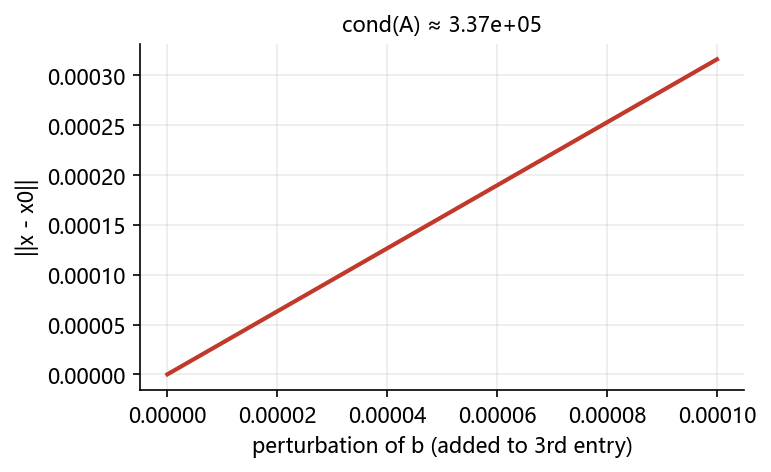
\includegraphics[keepaspectratio,alt={条件数敏感性}]{figures/01-numpy/cond_sensitivity.png}}
\caption{条件数敏感性}
\end{figure}

\textbf{结论}：即使 \texttt{b} 的扰动非常小（\texttt{1e-4}
量级），解的变化也可能很大；工程中应尽量避免病态方程组，或换用更稳定的分解方法。

\begin{center}\rule{0.5\linewidth}{0.5pt}\end{center}

\subsection{3.3 矩阵分解}\label{ux77e9ux9635ux5206ux89e3}

\subsubsection{\texorpdfstring{3.3.1
特征值分解（\texttt{eig}）}{3.3.1 特征值分解（eig）}}\label{ux7279ux5f81ux503cux5206ux89e3eig}

只适用于\textbf{方阵}（且通常要求可对角化）：

\begin{Shaded}
\begin{Highlighting}[]
\NormalTok{A }\OperatorTok{=}\NormalTok{ np.array([[}\DecValTok{2}\NormalTok{, }\DecValTok{1}\NormalTok{], [}\DecValTok{1}\NormalTok{, }\DecValTok{2}\NormalTok{]])}
\NormalTok{w, v }\OperatorTok{=}\NormalTok{ np.linalg.eig(A)}
\BuiltInTok{print}\NormalTok{(w)          }\CommentTok{\# [3. 1.] 特征值}
\BuiltInTok{print}\NormalTok{(v)          }\CommentTok{\# 列向量为对应特征向量}
\BuiltInTok{print}\NormalTok{(A }\OperatorTok{@}\NormalTok{ v[:, }\DecValTok{0}\NormalTok{] }\OperatorTok{==}\NormalTok{ w[}\DecValTok{0}\NormalTok{] }\OperatorTok{*}\NormalTok{ v[:, }\DecValTok{0}\NormalTok{])   }\CommentTok{\# 验证 Av = λv}
\end{Highlighting}
\end{Shaded}

\subsubsection{3.3.2
奇异值分解（SVD）}\label{ux5947ux5f02ux503cux5206ux89e3svd}

对\textbf{任意矩阵}（包括非方阵）适用：

\begin{Shaded}
\begin{Highlighting}[]
\NormalTok{M }\OperatorTok{=}\NormalTok{ np.array([[}\DecValTok{1}\NormalTok{, }\DecValTok{2}\NormalTok{], [}\DecValTok{3}\NormalTok{, }\DecValTok{4}\NormalTok{], [}\DecValTok{5}\NormalTok{, }\DecValTok{6}\NormalTok{]], dtype}\OperatorTok{=}\BuiltInTok{float}\NormalTok{)}
\NormalTok{U, S, Vt }\OperatorTok{=}\NormalTok{ np.linalg.svd(M, full\_matrices}\OperatorTok{=}\VariableTok{False}\NormalTok{)}
\BuiltInTok{print}\NormalTok{(U.shape, S.shape, Vt.shape)   }\CommentTok{\# (3,2) (2,) (2,2)}
\BuiltInTok{print}\NormalTok{(S)                            }\CommentTok{\# 奇异值（降序）}
\BuiltInTok{print}\NormalTok{(U }\OperatorTok{@}\NormalTok{ np.diag(S) }\OperatorTok{@}\NormalTok{ Vt)          }\CommentTok{\# 重构 ≈ M}
\end{Highlighting}
\end{Shaded}

\textbf{为什么重要}：奇异值从大到小排列，只保留前 \texttt{k}
个奇异值即可得到``最优低秩近似''，这是数据压缩、降维（PCA）、图像压缩的基础。见
\href{./05-综合案例.md}{05 综合案例}。

\begin{figure}
\centering
\pandocbounded{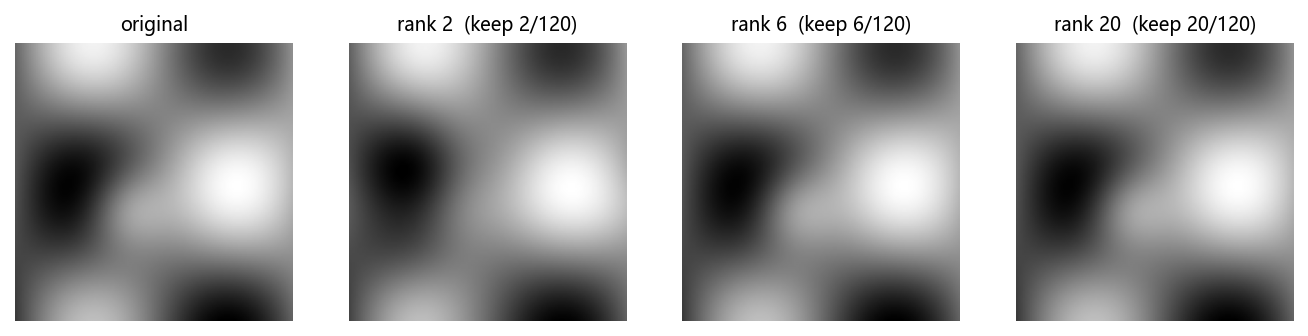
\includegraphics[keepaspectratio,alt={SVD 压缩示例}]{figures/01-numpy/svd_compression.png}}
\caption{SVD 压缩示例}
\end{figure}

\subsubsection{3.3.3 Cholesky 分解}\label{cholesky-ux5206ux89e3}

要求矩阵\textbf{对称正定}：

\begin{Shaded}
\begin{Highlighting}[]
\NormalTok{A }\OperatorTok{=}\NormalTok{ np.array([[}\FloatTok{4.}\NormalTok{, }\FloatTok{2.}\NormalTok{], [}\FloatTok{2.}\NormalTok{, }\FloatTok{3.}\NormalTok{]])}
\NormalTok{L }\OperatorTok{=}\NormalTok{ np.linalg.cholesky(A)}
\BuiltInTok{print}\NormalTok{(L)          }\CommentTok{\# [[2. 0. ][1. 1.4142]]}
\BuiltInTok{print}\NormalTok{(L }\OperatorTok{@}\NormalTok{ L.T)    }\CommentTok{\# ≈ A}
\end{Highlighting}
\end{Shaded}

\subsubsection{3.3.4 QR 分解}\label{qr-ux5206ux89e3}

\begin{Shaded}
\begin{Highlighting}[]
\NormalTok{A }\OperatorTok{=}\NormalTok{ np.array([[}\FloatTok{12.}\NormalTok{, }\OperatorTok{{-}}\FloatTok{51.}\NormalTok{], [}\FloatTok{6.}\NormalTok{, }\FloatTok{167.}\NormalTok{], [}\OperatorTok{{-}}\FloatTok{4.}\NormalTok{, }\FloatTok{24.}\NormalTok{]])}
\NormalTok{Q, R }\OperatorTok{=}\NormalTok{ np.linalg.qr(A)}
\BuiltInTok{print}\NormalTok{(Q.shape, R.shape)   }\CommentTok{\# (3,2) (2,2)}
\BuiltInTok{print}\NormalTok{(np.allclose(Q }\OperatorTok{@}\NormalTok{ R, A))   }\CommentTok{\# True}
\end{Highlighting}
\end{Shaded}

QR 在最小二乘、特征值算法稳定实现中广泛使用。

\begin{center}\rule{0.5\linewidth}{0.5pt}\end{center}

\subsection{常见误区}\label{ux5e38ux89c1ux8befux533a-2}

\begin{enumerate}
\def\labelenumi{\arabic{enumi}.}
\tightlist
\item
  \textbf{对非方阵用 \texttt{inv}}：应使用 \texttt{pinv} 或
  \texttt{lstsq}。
\item
  \textbf{认为 \texttt{eig}
  对任意矩阵都可用}：特征值分解只对方阵；非方阵用 SVD。
\item
  \textbf{忽略条件数}：\texttt{solve} 计算成功 ≠ 解可靠，先看
  \texttt{cond}。
\item
  \textbf{SVD 返回的 \texttt{S} 不是对角矩阵}：需要 \texttt{np.diag(S)}
  构造。
\item
  \textbf{\texttt{full\_matrices=False}
  与非默认的区别}：不关心零奇异值/补全正交基时，用
  \texttt{full\_matrices=False} 更省内存。
\end{enumerate}

\subsection{思考题}\label{ux601dux8003ux9898-2}

\begin{enumerate}
\def\labelenumi{\arabic{enumi}.}
\tightlist
\item
  为什么 \texttt{cond(A)} 很大时，\texttt{np.linalg.solve(A,\ b)}
  的结果可能仍``看起来正常''？
\item
  SVD 的 \texttt{U}、\texttt{Vt} 与 \texttt{eig}
  的特征向量有什么联系（提示：\texttt{A\^{}T\ A}）？
\item
  若只保留前 1 个奇异值做近似，误差如何估计？
\end{enumerate}

\subsection{动手练习（详见
lab）}\label{ux52a8ux624bux7ec3ux4e60ux8be6ux89c1-lab-2}

\begin{itemize}
\tightlist
\item
  解一个 \(4\times4\) 线性方程组 3 组（含病态）并比较解；
\item
  对 10×5 矩阵做 SVD，比较 rank 1/3/5 重构误差；
\item
  用 Cholesky 验证正定矩阵的分解唯一性。
\end{itemize}

\subsection{延伸阅读}\label{ux5ef6ux4f38ux9605ux8bfb-2}

\begin{itemize}
\tightlist
\item
  NumPy 官方 linalg
  参考：https://numpy.org/doc/stable/reference/routines.linalg.html
\item
  NumPy 官方广播与 linalg
  教程：https://numpy.org/doc/stable/reference/routines.linalg.html\#module-numpy.linalg
\item
  SciPy Lecture Notes --
  线性代数：https://scipy-lectures.org/intro/scipy.html\#linear-algebra
\end{itemize}

\section{04
多项式与拟合：poly1d、求根与最小二乘拟合}\label{ux591aux9879ux5f0fux4e0eux62dfux5408poly1dux6c42ux6839ux4e0eux6700ux5c0fux4e8cux4e58ux62dfux5408}

\begin{quote}
本节对应原版 1.4 的内容，并增补学习目标、常见误区、思考题与延伸阅读。
配套图：\texttt{figures/01-numpy/polyfit.png}。
\end{quote}

\subsection{本节目标}\label{ux672cux8282ux76eeux6807-3}

\begin{itemize}
\tightlist
\item
  会用 \texttt{np.poly1d} 构造、求值、加减乘除多项式；
\item
  会求导（\texttt{deriv}）、积分（\texttt{integ}）、求根（\texttt{np.roots}）；
\item
  会用 \texttt{np.polyfit} / \texttt{np.polyval}
  做最小二乘拟合，并理解``过拟合''现象；
\item
  知道新版 \texttt{np.polynomial.Polynomial} 的方向（便于迁移）。
\end{itemize}

\subsection{先修}\label{ux5148ux4fee-3}

\begin{itemize}
\tightlist
\item
  01 数组基础、02 数组运算；了解``多项式系数按最高次到常数排列''。
\end{itemize}

\begin{center}\rule{0.5\linewidth}{0.5pt}\end{center}

\subsection{4.1
多项式的构造与运算}\label{ux591aux9879ux5f0fux7684ux6784ux9020ux4e0eux8fd0ux7b97}

\begin{Shaded}
\begin{Highlighting}[]
\ImportTok{import}\NormalTok{ numpy }\ImportTok{as}\NormalTok{ np}

\CommentTok{\#\# 2x\^{}2 + 3x + 1}
\NormalTok{p }\OperatorTok{=}\NormalTok{ np.poly1d([}\DecValTok{2}\NormalTok{, }\DecValTok{3}\NormalTok{, }\DecValTok{1}\NormalTok{])}
\BuiltInTok{print}\NormalTok{(p)          }\CommentTok{\# 2 x\^{}2 + 3 x + 1}
\BuiltInTok{print}\NormalTok{(p(}\DecValTok{5}\NormalTok{))       }\CommentTok{\# 66}
\end{Highlighting}
\end{Shaded}

\begin{Shaded}
\begin{Highlighting}[]
\NormalTok{   2}
\NormalTok{2 x + 3 x + 1}
\NormalTok{66}
\end{Highlighting}
\end{Shaded}

\subsubsection{4.1.1 四则运算}\label{ux56dbux5219ux8fd0ux7b97}

\begin{Shaded}
\begin{Highlighting}[]
\NormalTok{p }\OperatorTok{=}\NormalTok{ np.poly1d([}\DecValTok{2}\NormalTok{, }\DecValTok{3}\NormalTok{, }\DecValTok{1}\NormalTok{])       }\CommentTok{\# 2x\^{}2+3x+1}
\NormalTok{q }\OperatorTok{=}\NormalTok{ np.poly1d([}\DecValTok{1}\NormalTok{, }\OperatorTok{{-}}\DecValTok{1}\NormalTok{])         }\CommentTok{\# x {-} 1}

\BuiltInTok{print}\NormalTok{(p }\OperatorTok{+}\NormalTok{ q)      }\CommentTok{\# 加法}
\BuiltInTok{print}\NormalTok{(p }\OperatorTok{{-}}\NormalTok{ q)      }\CommentTok{\# 减法}
\BuiltInTok{print}\NormalTok{(p }\OperatorTok{*}\NormalTok{ q)      }\CommentTok{\# 乘法（系数卷积）}
\BuiltInTok{print}\NormalTok{(p }\OperatorTok{/}\NormalTok{ q)      }\CommentTok{\# 除法 → (商, 余数) 元组}
\end{Highlighting}
\end{Shaded}

\begin{Shaded}
\begin{Highlighting}[]
\NormalTok{quotient, remainder }\OperatorTok{=}\NormalTok{ p }\OperatorTok{/}\NormalTok{ q    }\CommentTok{\# poly1d 直接除返回 (商, 余数) 元组}
\BuiltInTok{print}\NormalTok{(quotient)   }\CommentTok{\# 商}
\BuiltInTok{print}\NormalTok{(remainder)  }\CommentTok{\# 余数}

\CommentTok{\#\# 也可用 numpy.polydiv（传入系数）}
\NormalTok{q\_, r\_ }\OperatorTok{=}\NormalTok{ np.polydiv(p.coeffs, q.coeffs)}
\end{Highlighting}
\end{Shaded}

\subsubsection{4.1.2 求导与积分}\label{ux6c42ux5bfcux4e0eux79efux5206}

\begin{Shaded}
\begin{Highlighting}[]
\NormalTok{p }\OperatorTok{=}\NormalTok{ np.poly1d([}\DecValTok{2}\NormalTok{, }\DecValTok{3}\NormalTok{, }\DecValTok{1}\NormalTok{])}
\BuiltInTok{print}\NormalTok{(p.deriv())      }\CommentTok{\# 4x + 3}
\BuiltInTok{print}\NormalTok{(p.deriv(}\DecValTok{2}\NormalTok{))     }\CommentTok{\# 二阶导}
\BuiltInTok{print}\NormalTok{(p.integ())      }\CommentTok{\# 0.6667x\^{}3 + 1.5x\^{}2 + x（常数默认为 0）}
\BuiltInTok{print}\NormalTok{(p.integ(m}\OperatorTok{=}\DecValTok{2}\NormalTok{))   }\CommentTok{\# 二重积分}
\end{Highlighting}
\end{Shaded}

\subsubsection{4.1.3 系数与求根}\label{ux7cfbux6570ux4e0eux6c42ux6839}

\begin{Shaded}
\begin{Highlighting}[]
\NormalTok{p }\OperatorTok{=}\NormalTok{ np.poly1d([}\DecValTok{1}\NormalTok{, }\OperatorTok{{-}}\DecValTok{3}\NormalTok{, }\DecValTok{2}\NormalTok{])     }\CommentTok{\# x\^{}2 {-} 3x + 2}
\BuiltInTok{print}\NormalTok{(p.coeffs)               }\CommentTok{\# [ 1. {-}3.  2.]}
\BuiltInTok{print}\NormalTok{(p.c)                    }\CommentTok{\# 按降幂的系数}
\NormalTok{np.roots(p)                   }\CommentTok{\# [2. 1.]}
\end{Highlighting}
\end{Shaded}

\begin{quote}
\texttt{np.roots}
也支持直接传系数数组：\texttt{np.roots({[}1,\ -3,\ 2{]})}。
\end{quote}

\begin{center}\rule{0.5\linewidth}{0.5pt}\end{center}

\subsection{4.2
最小二乘拟合：polyfit}\label{ux6700ux5c0fux4e8cux4e58ux62dfux5408polyfit}

\begin{Shaded}
\begin{Highlighting}[]
\NormalTok{x }\OperatorTok{=}\NormalTok{ np.array([}\DecValTok{0}\NormalTok{, }\DecValTok{1}\NormalTok{, }\DecValTok{2}\NormalTok{, }\DecValTok{3}\NormalTok{, }\DecValTok{4}\NormalTok{], dtype}\OperatorTok{=}\BuiltInTok{float}\NormalTok{)}
\NormalTok{y }\OperatorTok{=}\NormalTok{ np.array([}\DecValTok{1}\NormalTok{, }\DecValTok{2}\NormalTok{, }\DecValTok{9}\NormalTok{, }\DecValTok{28}\NormalTok{, }\DecValTok{65}\NormalTok{], dtype}\OperatorTok{=}\BuiltInTok{float}\NormalTok{)   }\CommentTok{\# 恰好是 x\^{}3 + 1}

\NormalTok{coef }\OperatorTok{=}\NormalTok{ np.polyfit(x, y, }\DecValTok{3}\NormalTok{)       }\CommentTok{\# 3 次多项式最小二乘}
\BuiltInTok{print}\NormalTok{(coef)                      }\CommentTok{\# [ 1.  0. {-}0.  1.]}
\NormalTok{p }\OperatorTok{=}\NormalTok{ np.poly1d(coef)}
\BuiltInTok{print}\NormalTok{(p)                         }\CommentTok{\# 1 x\^{}3 + 0 x\^{}2 + 0 x + 1}
\BuiltInTok{print}\NormalTok{(np.polyval(coef, }\FloatTok{2.5}\NormalTok{))     }\CommentTok{\# 16.625}
\end{Highlighting}
\end{Shaded}

\textbf{含噪声数据的拟合与过拟合}：

\begin{Shaded}
\begin{Highlighting}[]
\ImportTok{import}\NormalTok{ numpy }\ImportTok{as}\NormalTok{ np}
\ImportTok{import}\NormalTok{ matplotlib.pyplot }\ImportTok{as}\NormalTok{ plt}

\NormalTok{np.random.seed(}\DecValTok{7}\NormalTok{)}
\KeywordTok{def}\NormalTok{ f(x): }\ControlFlowTok{return} \DecValTok{2} \OperatorTok{*}\NormalTok{ x }\OperatorTok{**} \DecValTok{2} \OperatorTok{{-}} \DecValTok{3} \OperatorTok{*}\NormalTok{ x }\OperatorTok{+} \DecValTok{1}
\NormalTok{x }\OperatorTok{=}\NormalTok{ np.linspace(}\OperatorTok{{-}}\DecValTok{2}\NormalTok{, }\DecValTok{3}\NormalTok{, }\DecValTok{40}\NormalTok{)}
\NormalTok{y }\OperatorTok{=}\NormalTok{ f(x) }\OperatorTok{+}\NormalTok{ np.random.normal(}\DecValTok{0}\NormalTok{, }\DecValTok{2}\NormalTok{, x.size)   }\CommentTok{\# 加噪声}

\ControlFlowTok{for}\NormalTok{ deg }\KeywordTok{in}\NormalTok{ (}\DecValTok{1}\NormalTok{, }\DecValTok{3}\NormalTok{, }\DecValTok{5}\NormalTok{):}
\NormalTok{    coef }\OperatorTok{=}\NormalTok{ np.polyfit(x, y, deg)}
    \BuiltInTok{print}\NormalTok{(deg, }\StringTok{":"}\NormalTok{, coef)}

\CommentTok{\#\# 绘图}
\NormalTok{xs }\OperatorTok{=}\NormalTok{ np.linspace(}\OperatorTok{{-}}\DecValTok{2}\NormalTok{, }\DecValTok{3}\NormalTok{, }\DecValTok{200}\NormalTok{)}
\NormalTok{plt.scatter(x, y, s}\OperatorTok{=}\DecValTok{16}\NormalTok{, label}\OperatorTok{=}\StringTok{"data"}\NormalTok{)}
\ControlFlowTok{for}\NormalTok{ deg, c, ls }\KeywordTok{in}\NormalTok{ [(}\DecValTok{1}\NormalTok{, }\StringTok{"grey"}\NormalTok{, }\StringTok{"{-}{-}"}\NormalTok{), (}\DecValTok{3}\NormalTok{, }\StringTok{"orange"}\NormalTok{, }\StringTok{"{-}."}\NormalTok{), (}\DecValTok{5}\NormalTok{, }\StringTok{"green"}\NormalTok{, }\StringTok{"{-}"}\NormalTok{)]:}
\NormalTok{    plt.plot(xs, np.polyval(np.polyfit(x, y, deg), xs), c}\OperatorTok{=}\NormalTok{c, ls}\OperatorTok{=}\NormalTok{ls, label}\OperatorTok{=}\SpecialStringTok{f"deg }\SpecialCharTok{\{}\NormalTok{deg}\SpecialCharTok{\}}\SpecialStringTok{"}\NormalTok{)}
\NormalTok{plt.legend()}\OperatorTok{;}\NormalTok{ plt.savefig(}\StringTok{"poly\_fit\_demo.png"}\NormalTok{)}
\end{Highlighting}
\end{Shaded}

\begin{figure}
\centering
\pandocbounded{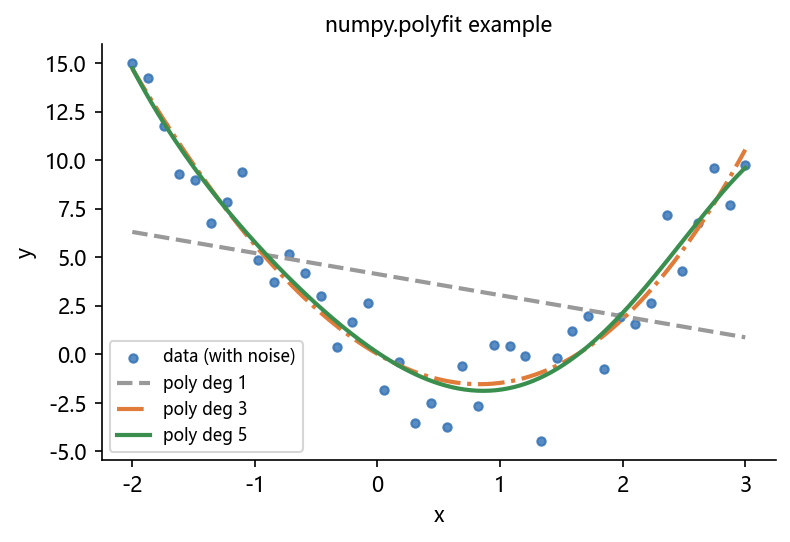
\includegraphics[keepaspectratio,alt={polyfit 示例}]{figures/01-numpy/polyfit.png}}
\caption{polyfit 示例}
\end{figure}

\textbf{观察}：次数越高，拟合曲线越可能贴近噪声（过拟合）；次数过低则拟合不足。选择次数可用交叉验证或残差分析，而不是盲目升高次数。

\begin{center}\rule{0.5\linewidth}{0.5pt}\end{center}

\subsection{4.3
新版多项式接口（了解）}\label{ux65b0ux7248ux591aux9879ux5f0fux63a5ux53e3ux4e86ux89e3}

NumPy 1.x 之后的 \texttt{np.polynomial} 提供更现代、更稳定的
\texttt{Polynomial} / \texttt{Chebyshev} 等类：

\begin{Shaded}
\begin{Highlighting}[]
\ImportTok{from}\NormalTok{ numpy.polynomial }\ImportTok{import}\NormalTok{ Polynomial}
\NormalTok{p }\OperatorTok{=}\NormalTok{ Polynomial([}\DecValTok{1}\NormalTok{, }\DecValTok{3}\NormalTok{, }\DecValTok{2}\NormalTok{])     }\CommentTok{\# 注意：系数从常数项开始！}
\BuiltInTok{print}\NormalTok{(p(}\DecValTok{2}\NormalTok{))                   }\CommentTok{\# 1 + 3*2 + 2*2\^{}2 = 15}
\BuiltInTok{print}\NormalTok{(p.roots())}
\end{Highlighting}
\end{Shaded}

\begin{quote}
\texttt{np.poly1d}
是旧接口（系数降幂、基于\texttt{np.poly}），大量教程/教材仍在使用；新代码可优先考虑
\texttt{np.polynomial}。本讲义两者都给出，以兼容常见场景。
\end{quote}

\begin{center}\rule{0.5\linewidth}{0.5pt}\end{center}

\subsection{常见误区}\label{ux5e38ux89c1ux8befux533a-3}

\begin{enumerate}
\def\labelenumi{\arabic{enumi}.}
\tightlist
\item
  \textbf{系数顺序搞反}：\texttt{poly1d({[}a,\ b,\ c{]})} 表示
  \(a x^2 + b x + c\)；\texttt{np.polynomial.Polynomial}
  则是常数项在前。
\item
  \textbf{\texttt{polyfit} 次数过高}：数据少时高次多项式会震荡/过拟合。
\item
  \textbf{忘记噪声与残差}：拟合不是``解释唯一真理''，要报告残差与预测区间。
\item
  \textbf{把 \texttt{polyfit}
  当精确解}：它是数值最小二乘，数据含噪声时系数有误差。
\end{enumerate}

\subsection{思考题}\label{ux601dux8003ux9898-3}

\begin{enumerate}
\def\labelenumi{\arabic{enumi}.}
\tightlist
\item
  \(n\) 个数据点做 \(n-1\) 次多项式拟合会出现什么现象？为什么？
\item
  \texttt{polyfit} 与 \texttt{lstsq} 的关系是什么？
\item
  如何判断``次数挑对了''？
\end{enumerate}

\subsection{动手练习（详见
lab）}\label{ux52a8ux624bux7ec3ux4e60ux8be6ux89c1-lab-3}

\begin{itemize}
\tightlist
\item
  对 \(y = 0.5x^3 - 2x + 1 + \varepsilon\) 的 30 个噪声点，分别拟合
  1/3/5 次，比较残差与测试误差；
\item
  用 \texttt{poly1d} 求 \(x^4 - 5x^2 + 4\) 的根，并验证代入为 0。
\end{itemize}

\subsection{延伸阅读}\label{ux5ef6ux4f38ux9605ux8bfb-3}

\begin{itemize}
\tightlist
\item
  NumPy 官方 polynomial
  文档：https://numpy.org/doc/stable/reference/routines.polynomials.html
\item
  NumPy 官方 polyfit
  说明：https://numpy.org/doc/stable/reference/generated/numpy.polyfit.html
\item
  SciPy Lecture Notes --
  最小二乘：https://scipy-lectures.org/intro/scipy.html\#least-squares-approximation
\end{itemize}

\section{05 综合案例：SVD
图像压缩与实验数据拟合}\label{ux7efcux5408ux6848ux4f8bsvd-ux56feux50cfux538bux7f29ux4e0eux5b9eux9a8cux6570ux636eux62dfux5408}

\begin{quote}
本章新增综合案例，用于把 01--04 的知识串起来：\textbf{形状/广播 +
线性代数 + 拟合 + 可视化}。 所有代码均可在 NumPy ≥ 1.24
环境直接运行；配图由 \texttt{build/make\_chap1\_figures.py} 生成。
\end{quote}

\subsection{案例 1：用 SVD
压缩一张``图像''}\label{ux6848ux4f8b-1ux7528-svd-ux538bux7f29ux4e00ux5f20ux56feux50cf}

\subsubsection{背景}\label{ux80ccux666f}

一张 \(m \times n\) 的灰度图可看作矩阵。SVD 给出

\[
A = U \Sigma V^T,\qquad U\in\mathbb{R}^{m\times r},\ \Sigma\in\mathbb{R}^{r\times r},\ V\in\mathbb{R}^{n\times r}
\]

只保留前 \(k\) 个奇异值，得到低秩近似

\[
A_k = U_{:,1:k}\ \Sigma_{1:k,1:k}\ V_{1:k,:}^T
\]

存储量从 \(m n\) 减少到 \(k(m+n+1)\)，当 \(k\ll \min(m,n)\) 时压缩明显。

\subsubsection{代码：生成合成图像并做低秩近似}\label{ux4ee3ux7801ux751fux6210ux5408ux6210ux56feux50cfux5e76ux505aux4f4eux79e9ux8fd1ux4f3c}

\begin{Shaded}
\begin{Highlighting}[]
\ImportTok{import}\NormalTok{ numpy }\ImportTok{as}\NormalTok{ np}
\ImportTok{import}\NormalTok{ matplotlib.pyplot }\ImportTok{as}\NormalTok{ plt}

\CommentTok{\#\# 1) 生成一张“灰度图”（120x120，含图案与明暗渐变）}
\NormalTok{x }\OperatorTok{=}\NormalTok{ np.linspace(}\DecValTok{0}\NormalTok{, }\DecValTok{1}\NormalTok{, }\DecValTok{120}\NormalTok{)}\OperatorTok{;}\NormalTok{ y }\OperatorTok{=}\NormalTok{ np.linspace(}\DecValTok{0}\NormalTok{, }\DecValTok{1}\NormalTok{, }\DecValTok{120}\NormalTok{)}
\NormalTok{X, Y }\OperatorTok{=}\NormalTok{ np.meshgrid(x, y)}
\NormalTok{img }\OperatorTok{=}\NormalTok{ (np.sin(}\DecValTok{6} \OperatorTok{*}\NormalTok{ X) }\OperatorTok{*}\NormalTok{ np.cos(}\DecValTok{6} \OperatorTok{*}\NormalTok{ Y)}
       \OperatorTok{+}\NormalTok{ np.exp(}\OperatorTok{{-}}\NormalTok{((X }\OperatorTok{{-}} \FloatTok{0.4}\NormalTok{) }\OperatorTok{**} \DecValTok{2} \OperatorTok{+}\NormalTok{ (Y }\OperatorTok{{-}} \FloatTok{0.6}\NormalTok{) }\OperatorTok{**} \DecValTok{2}\NormalTok{) }\OperatorTok{*} \DecValTok{40}\NormalTok{)}
       \OperatorTok{+} \FloatTok{0.6} \OperatorTok{*}\NormalTok{ X }\OperatorTok{{-}} \FloatTok{0.4} \OperatorTok{*}\NormalTok{ Y)}
\NormalTok{img }\OperatorTok{=}\NormalTok{ (img }\OperatorTok{{-}}\NormalTok{ img.}\BuiltInTok{min}\NormalTok{()) }\OperatorTok{/}\NormalTok{ (img.}\BuiltInTok{max}\NormalTok{() }\OperatorTok{{-}}\NormalTok{ img.}\BuiltInTok{min}\NormalTok{())}

\CommentTok{\#\# 2) SVD}
\NormalTok{U, S, Vt }\OperatorTok{=}\NormalTok{ np.linalg.svd(img, full\_matrices}\OperatorTok{=}\VariableTok{False}\NormalTok{)}

\CommentTok{\#\# 3) 不同秩的重建与误差}
\ControlFlowTok{for}\NormalTok{ k }\KeywordTok{in}\NormalTok{ (}\DecValTok{2}\NormalTok{, }\DecValTok{6}\NormalTok{, }\DecValTok{20}\NormalTok{):}
\NormalTok{    A\_k }\OperatorTok{=}\NormalTok{ U[:, :k] }\OperatorTok{@}\NormalTok{ np.diag(S[:k]) }\OperatorTok{@}\NormalTok{ Vt[:k, :]}
\NormalTok{    mse }\OperatorTok{=}\NormalTok{ np.mean((img }\OperatorTok{{-}}\NormalTok{ A\_k) }\OperatorTok{**} \DecValTok{2}\NormalTok{)}
\NormalTok{    params }\OperatorTok{=}\NormalTok{ k }\OperatorTok{*}\NormalTok{ (img.shape[}\DecValTok{0}\NormalTok{] }\OperatorTok{+} \DecValTok{1} \OperatorTok{+}\NormalTok{ img.shape[}\DecValTok{1}\NormalTok{])}
    \BuiltInTok{print}\NormalTok{(}\SpecialStringTok{f"rank=}\SpecialCharTok{\{}\NormalTok{k}\SpecialCharTok{:2d\}}\SpecialStringTok{  MSE=}\SpecialCharTok{\{}\NormalTok{mse}\SpecialCharTok{:.5f\}}\SpecialStringTok{  存储量=}\SpecialCharTok{\{}\NormalTok{params}\SpecialCharTok{\}}\SpecialStringTok{ / 原图=}\SpecialCharTok{\{}\NormalTok{img}\SpecialCharTok{.}\NormalTok{size}\SpecialCharTok{\}}\SpecialStringTok{ "}
          \SpecialStringTok{f"(}\SpecialCharTok{\{}\DecValTok{100}\OperatorTok{*}\NormalTok{params}\OperatorTok{/}\NormalTok{img}\SpecialCharTok{.}\NormalTok{size}\SpecialCharTok{:.1f\}}\SpecialStringTok{\%)"}\NormalTok{)}
\end{Highlighting}
\end{Shaded}

\begin{Shaded}
\begin{Highlighting}[]
\NormalTok{rank= 2  MSE=0.00087  存储量=482 / 原图=14400 (3.3\%)}
\NormalTok{rank= 6  MSE=0.00000  存储量=1446 / 原图=14400 (10.0\%)}
\NormalTok{rank=20  MSE=0.00000  存储量=4820 / 原图=14400 (33.5\%)}
\end{Highlighting}
\end{Shaded}

\begin{figure}
\centering
\pandocbounded{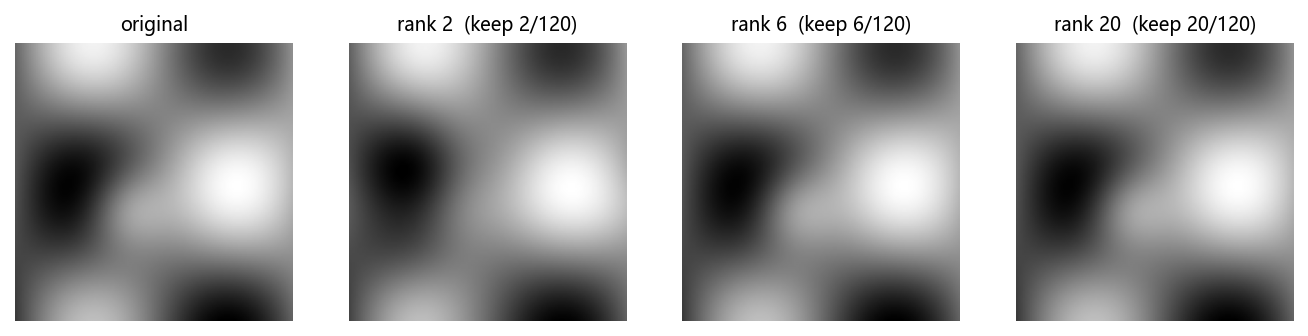
\includegraphics[keepaspectratio,alt={SVD 图像压缩}]{figures/01-numpy/svd_compression.png}}
\caption{SVD 图像压缩}
\end{figure}

\subsubsection{分析}\label{ux5206ux6790}

\begin{itemize}
\tightlist
\item
  rank=2 时仅用 3.3\% 的存储量，MSE≈0.0009（肉眼几乎无差别）；
\item
  rank=6 之后误差已低于打印精度；
\item
  说明\textbf{自然图像的能量高度集中在前几个奇异值}------这正是图像压缩、PCA、数据降维的共同原理。
\end{itemize}

\subsubsection{拓展任务}\label{ux62d3ux5c55ux4efbux52a1}

\begin{enumerate}
\def\labelenumi{\arabic{enumi}.}
\tightlist
\item
  用
  \texttt{np.linalg.norm(img\ -\ A\_k,\ \textquotesingle{}fro\textquotesingle{})}
  计算相对误差；
\item
  对一张真实图片（PIL 读取灰度化）重复实验，观察``压缩率 vs 视觉质量'';
\item
  把 \texttt{img} 换成随机噪声图，观察奇异值衰减是否还那么快？为什么？
\end{enumerate}

\begin{center}\rule{0.5\linewidth}{0.5pt}\end{center}

\subsection{案例
2：实验数据的最小二乘拟合}\label{ux6848ux4f8b-2ux5b9eux9a8cux6570ux636eux7684ux6700ux5c0fux4e8cux4e58ux62dfux5408}

\subsubsection{背景}\label{ux80ccux666f-1}

物理实验得到一组 \((x_i, y_i)\)，理论公式是二次函数，但测量有噪声。用
\texttt{np.polyfit} 求 \(y = a x^2 + b x + c\)
的最佳系数，并评估拟合质量。

\subsubsection{代码}\label{ux4ee3ux7801}

\begin{Shaded}
\begin{Highlighting}[]
\ImportTok{import}\NormalTok{ numpy }\ImportTok{as}\NormalTok{ np}
\ImportTok{import}\NormalTok{ matplotlib.pyplot }\ImportTok{as}\NormalTok{ plt}

\NormalTok{np.random.seed(}\DecValTok{7}\NormalTok{)}
\KeywordTok{def}\NormalTok{ theory(x): }\ControlFlowTok{return} \DecValTok{2} \OperatorTok{*}\NormalTok{ x }\OperatorTok{**} \DecValTok{2} \OperatorTok{{-}} \DecValTok{3} \OperatorTok{*}\NormalTok{ x }\OperatorTok{+} \DecValTok{1}

\NormalTok{x }\OperatorTok{=}\NormalTok{ np.linspace(}\OperatorTok{{-}}\DecValTok{2}\NormalTok{, }\DecValTok{3}\NormalTok{, }\DecValTok{40}\NormalTok{)}
\NormalTok{y }\OperatorTok{=}\NormalTok{ theory(x) }\OperatorTok{+}\NormalTok{ np.random.normal(}\DecValTok{0}\NormalTok{, }\DecValTok{2}\NormalTok{, x.size)   }\CommentTok{\# 加噪声}

\NormalTok{coef2 }\OperatorTok{=}\NormalTok{ np.polyfit(x, y, }\DecValTok{2}\NormalTok{)      }\CommentTok{\# 二次拟合}
\NormalTok{coef5 }\OperatorTok{=}\NormalTok{ np.polyfit(x, y, }\DecValTok{5}\NormalTok{)      }\CommentTok{\# 五次拟合（对比）}
\BuiltInTok{print}\NormalTok{(}\StringTok{"二次系数 (a,b,c):"}\NormalTok{, np.}\BuiltInTok{round}\NormalTok{(coef2, }\DecValTok{3}\NormalTok{))}
\BuiltInTok{print}\NormalTok{(}\StringTok{"五次系数:"}\NormalTok{, np.}\BuiltInTok{round}\NormalTok{(coef5, }\DecValTok{3}\NormalTok{))}

\CommentTok{\#\# 残差（RMSE）}
\NormalTok{rmse2 }\OperatorTok{=}\NormalTok{ np.sqrt(np.mean((np.polyval(coef2, x) }\OperatorTok{{-}}\NormalTok{ y) }\OperatorTok{**} \DecValTok{2}\NormalTok{))}
\NormalTok{rmse5 }\OperatorTok{=}\NormalTok{ np.sqrt(np.mean((np.polyval(coef5, x) }\OperatorTok{{-}}\NormalTok{ y) }\OperatorTok{**} \DecValTok{2}\NormalTok{))}
\BuiltInTok{print}\NormalTok{(}\SpecialStringTok{f"RMSE(deg2)=}\SpecialCharTok{\{}\NormalTok{rmse2}\SpecialCharTok{:.3f\}}\SpecialStringTok{  RMSE(deg5)=}\SpecialCharTok{\{}\NormalTok{rmse5}\SpecialCharTok{:.3f\}}\SpecialStringTok{"}\NormalTok{)}
\end{Highlighting}
\end{Shaded}

\begin{Shaded}
\begin{Highlighting}[]
\NormalTok{二次系数 (a,b,c): [ 2.123 {-}3.231  0.616]}
\NormalTok{五次系数: [{-}0.010  0.210 {-}0.278  1.206 {-}2.469  1.162]}
\NormalTok{RMSE(deg2)=2.116  RMSE(deg5)=2.026}
\end{Highlighting}
\end{Shaded}

\subsubsection{分析}\label{ux5206ux6790-1}

\begin{itemize}
\tightlist
\item
  二次拟合系数接近真实值
  \((2, -3, 1)\)，说明模型设定正确时最小二乘能恢复参数；
\item
  五次拟合在训练数据上的 RMSE 略低（2.026 vs
  2.116），说明``次数越高越能贴合训练数据''------但这是\textbf{过拟合的征兆}；
\item
  把前 28 个点作训练、后 12
  个点作\textbf{独立测试}时：\texttt{deg2\ 测试\ RMSE≈3.11}，而
  \texttt{deg5\ 测试\ RMSE≈139.1}！过拟合在测试集上暴露无遗。因此选次数必须看独立测试集/交叉验证，而不是训练误差。
\end{itemize}

\begin{figure}
\centering
\pandocbounded{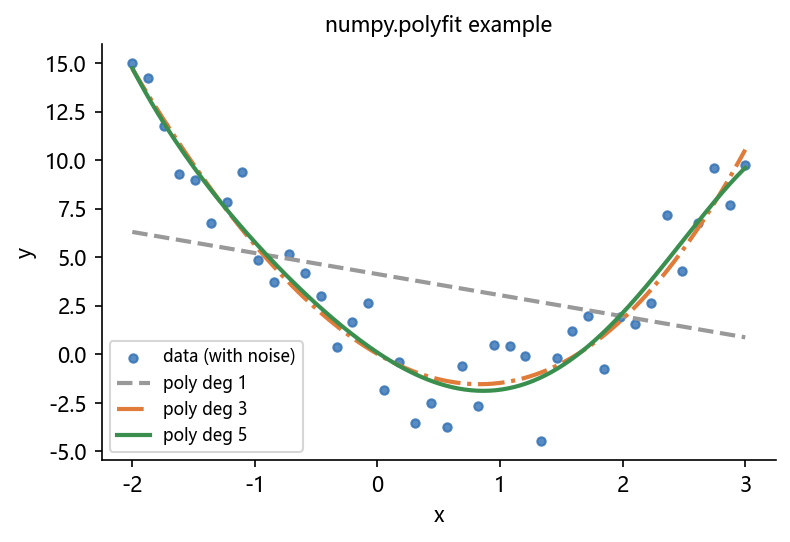
\includegraphics[keepaspectratio,alt={polyfit 示例}]{figures/01-numpy/polyfit.png}}
\caption{polyfit 示例}
\end{figure}

\subsubsection{拓展任务}\label{ux62d3ux5c55ux4efbux52a1-1}

\begin{enumerate}
\def\labelenumi{\arabic{enumi}.}
\tightlist
\item
  划分训练/测试集（如 70/30），比较 deg=2 与 deg=5 在测试集上的
  RMSE（本案例中 deg2≈3.11，deg5≈139.1）；
\item
  用 \texttt{np.linalg.lstsq} 重写拟合，体会与 \texttt{polyfit} 的关系；
\item
  打印 95\% 置信区间（提示：用 \texttt{np.polyfit} 的 cov 参数或
  scipy.stats）。
\end{enumerate}

\begin{center}\rule{0.5\linewidth}{0.5pt}\end{center}

\subsection{本章综合练习（上机任务）}\label{ux672cux7ae0ux7efcux5408ux7ec3ux4e60ux4e0aux673aux4efbux52a1}

\begin{enumerate}
\def\labelenumi{\arabic{enumi}.}
\tightlist
\item
  生成 50×50 的``数字 + 渐变''图案，用 rank = 1, 3, 5, 10 重构并绘制 2×2
  对比图；
\item
  构造 \(y = 3e^{-x} + 2 + \varepsilon\)
  的噪声数据，尝试多项式拟合（哪种次数更合理？），并给出误差曲线；
\item
  把案例 1 与案例 2 整理成一个 \texttt{.ipynb}，写一份 200
  字以内的结论。
\end{enumerate}

\subsection{延伸阅读}\label{ux5ef6ux4f38ux9605ux8bfb-4}

\begin{itemize}
\tightlist
\item
  NumPy 官方
  SVD：https://numpy.org/doc/stable/reference/generated/numpy.linalg.svd.html
\item
  SciPy
  相关低秩近似（scipy.sparse.linalg）：https://docs.scipy.org/doc/scipy/reference/sparse.linalg.html
\item
  scikit-learn PCA
  官方示例（下一章会用到）：https://scikit-learn.org/stable/auto\_examples/index.html\#decomposition
\end{itemize}

\section{06
常见误区与技巧}\label{ux5e38ux89c1ux8befux533aux4e0eux6280ux5de7}

\begin{quote}
本章为新增``查漏补缺''页：把学生最容易踩的坑集中列出，并给出正确的写法和性能技巧。
\end{quote}

\subsection{1.
高频误区速查表}\label{ux9ad8ux9891ux8befux533aux901fux67e5ux8868}

{\def\LTcaptype{none} % do not increment counter
\begin{longtable}[]{@{}
  >{\raggedright\arraybackslash}p{(\linewidth - 6\tabcolsep) * \real{0.2500}}
  >{\raggedright\arraybackslash}p{(\linewidth - 6\tabcolsep) * \real{0.2500}}
  >{\raggedright\arraybackslash}p{(\linewidth - 6\tabcolsep) * \real{0.2500}}
  >{\raggedright\arraybackslash}p{(\linewidth - 6\tabcolsep) * \real{0.2500}}@{}}
\toprule\noalign{}
\begin{minipage}[b]{\linewidth}\raggedright
\#
\end{minipage} & \begin{minipage}[b]{\linewidth}\raggedright
误区 / 错误写法
\end{minipage} & \begin{minipage}[b]{\linewidth}\raggedright
正确做法
\end{minipage} & \begin{minipage}[b]{\linewidth}\raggedright
原因
\end{minipage} \\
\midrule\noalign{}
\endhead
\bottomrule\noalign{}
\endlastfoot
1 & \texttt{A\ *\ B} 当矩阵乘法 & \texttt{A\ @\ B} 或
\texttt{np.matmul(A,\ B)} & \texttt{*} 是逐元素乘（ufunc） \\
2 & \texttt{np.zeros(2,\ 3)} & \texttt{np.zeros((2,\ 3))} &
形状要传元组，两个括号 \\
3 & 以为 \texttt{reshape} 是拷贝 & 需要独立数据用
\texttt{arr.reshape(...).copy()} & 连续内存的 reshape 是视图 \\
4 & \texttt{x{[}x\ \textgreater{}\ 0\ and\ x\ \textless{}\ 5{]}} &
\texttt{x{[}(x\ \textgreater{}\ 0)\ \&\ (x\ \textless{}\ 5){]}} &
数组布尔运算用 \texttt{\&}，且加括号 \\
5 & \texttt{len(a)} 猜数组维数 & \texttt{a.shape}、\texttt{a.ndim} &
\texttt{len} 只给第一维长度 \\
6 & 对非方阵 \texttt{np.linalg.inv} & \texttt{np.linalg.pinv} /
\texttt{lstsq} & 逆只定义于方阵 \\
7 & \texttt{np.linalg.svd(M)} 直接 \texttt{U@S@Vt} &
\texttt{U\ @\ np.diag(S)\ @\ Vt} & \texttt{S}
是奇异值向量，不是对角阵 \\
8 & 认为 \texttt{eig} 适用于任意矩阵 & 方阵用 \texttt{eig}，任意矩阵用
\texttt{svd} & \texttt{eig} 数学条件限制 \\
9 & \texttt{np.random.rand} 不设种子 &
\texttt{rng\ =\ np.random.default\_rng(42)} & 结果不可复现 \\
10 & 循环里 \texttt{np.append} & 预分配数组或列表收集 & 每次 append
都会新建数组 \\
11 & 混淆 \texttt{axis=0/1} & 记``消除哪一维就写哪一维'' &
\texttt{sum(axis=0)} 消行得列统计 \\
12 & 用 \texttt{astype} 想``改原数组'' & \texttt{arr.astype}
返回新数组；原地改 dtype 不可直接 & 类型转换是拷贝 \\
\end{longtable}
}

\subsection{2. 原理级难点：视图 vs
拷贝}\label{ux539fux7406ux7ea7ux96beux70b9ux89c6ux56fe-vs-ux62f7ux8d1d}

\begin{Shaded}
\begin{Highlighting}[]
\NormalTok{a }\OperatorTok{=}\NormalTok{ np.arange(}\DecValTok{6}\NormalTok{)}
\NormalTok{b }\OperatorTok{=}\NormalTok{ a.reshape(}\DecValTok{2}\NormalTok{, }\DecValTok{3}\NormalTok{)     }\CommentTok{\# 视图}
\NormalTok{b[}\DecValTok{0}\NormalTok{, }\DecValTok{0}\NormalTok{] }\OperatorTok{=} \DecValTok{99}
\BuiltInTok{print}\NormalTok{(a[}\DecValTok{0}\NormalTok{])             }\CommentTok{\# 99}

\NormalTok{c }\OperatorTok{=}\NormalTok{ a.copy()}
\NormalTok{c[}\DecValTok{0}\NormalTok{] }\OperatorTok{=} \DecValTok{0}                \CommentTok{\# 不影响 a}
\end{Highlighting}
\end{Shaded}

判断是否共享内存：

\begin{Shaded}
\begin{Highlighting}[]
\NormalTok{b.base }\KeywordTok{is}\NormalTok{ a              }\CommentTok{\# True → 视图}
\NormalTok{np.may\_share\_memory(a, b)  }\CommentTok{\# 更稳的检查}
\end{Highlighting}
\end{Shaded}

\textbf{为什么重要}：视图省内存、速度快；但并发修改或函数返回到别人手里时容易``隐形改数据''。对外返回数据前，若不想共享，显式
\texttt{.copy()}。

\subsection{3. 广播规则速记}\label{ux5e7fux64adux89c4ux5219ux901fux8bb0}

\begin{enumerate}
\def\labelenumi{\arabic{enumi}.}
\tightlist
\item
  从右往左对齐；
\item
  相同或一方为 1 → 兼容；
\item
  全部兼容 → 结果为各维最大；否则 \texttt{ValueError}。
\end{enumerate}

\begin{Shaded}
\begin{Highlighting}[]
\NormalTok{A }\OperatorTok{=}\NormalTok{ np.zeros((}\DecValTok{4}\NormalTok{, }\DecValTok{1}\NormalTok{, }\DecValTok{6}\NormalTok{))}
\NormalTok{B }\OperatorTok{=}\NormalTok{ np.zeros((}\DecValTok{3}\NormalTok{, }\DecValTok{6}\NormalTok{))}
\ControlFlowTok{try}\NormalTok{:}
    \BuiltInTok{print}\NormalTok{((A }\OperatorTok{+}\NormalTok{ B).shape)     }\CommentTok{\# (4, 3, 6)，B 自动补成 (1,3,6)}
\ControlFlowTok{except} \PreprocessorTok{ValueError} \ImportTok{as}\NormalTok{ e:}
    \BuiltInTok{print}\NormalTok{(}\StringTok{"广播失败："}\NormalTok{, e)}
\end{Highlighting}
\end{Shaded}

\begin{quote}
注意：\texttt{(3,)\ +\ (4,)} 不兼容；\texttt{(3,1)\ +\ (3,)}
也不兼容（末尾 1 vs 3）。想``列向量与行向量做外积''要用
\texttt{(3,1)\ +\ (1,3)}。
\end{quote}

\subsection{4. 性能技巧}\label{ux6027ux80fdux6280ux5de7}

\begin{itemize}
\item
  \textbf{向量化优先}：能一次
  \texttt{a{[}np.newaxis,\ :{]}\ +\ b{[}:,\ np.newaxis{]}}
  就不要双重循环；
\item
  \textbf{\texttt{out=} 原地计算}：\texttt{np.add(a,\ b,\ out=a)}
  避免额外分配；
\item
  \textbf{\texttt{in-place} 算术}：\texttt{a\ +=\ b}（注意类型安全）；
\item
  \textbf{\texttt{einsum}
  表达张量收缩}：\texttt{np.einsum(\textquotesingle{}ik,kj-\textgreater{}ij\textquotesingle{},\ A,\ B)}
  既是矩阵乘，也能表达更复杂收缩且减少中间数组；
\item
  \textbf{\texttt{np.lib.stride\_tricks.sliding\_window\_view}}
  做滑窗（移动平均/卷积）时避免显式复制：

\begin{Shaded}
\begin{Highlighting}[]
\NormalTok{x }\OperatorTok{=}\NormalTok{ np.arange(}\DecValTok{10}\NormalTok{)}
\NormalTok{w }\OperatorTok{=}\NormalTok{ np.lib.stride\_tricks.sliding\_window\_view(x, }\DecValTok{3}\NormalTok{)}
\BuiltInTok{print}\NormalTok{(w.mean(axis}\OperatorTok{=}\DecValTok{1}\NormalTok{))   }\CommentTok{\# 窗口大小为 3 的移动平均}
\end{Highlighting}
\end{Shaded}
\item
  \textbf{大数组用 \texttt{np.savez\_compressed}} 存储；文本
  \texttt{savetxt} 慢且丢精度。
\end{itemize}

\subsection{5. 调试建议}\label{ux8c03ux8bd5ux5efaux8bae}

\begin{enumerate}
\def\labelenumi{\arabic{enumi}.}
\tightlist
\item
  出错先打印 \texttt{shape} / \texttt{dtype}，再用 \texttt{np.allclose}
  比较；
\item
  用 \texttt{np.set\_printoptions(precision=4,\ suppress=True)}
  让输出可读；
\item
  复杂布尔条件拆成中间变量（\texttt{mask1\ =\ ...;\ mask2\ =\ ...}）；
\item
  随机/拟合问题\textbf{固定种子}，便于复现与讨论；
\item
  用 \texttt{np.isnan} / \texttt{np.isinf} 检查异常值。
\end{enumerate}

\subsection{6.
本章小结（自测）}\label{ux672cux7ae0ux5c0fux7ed3ux81eaux6d4b}

\begin{itemize}
\tightlist
\item[$\square$]
  能解释 \texttt{dtype} 与 \texttt{itemsize}；
\item[$\square$]
  能说出 \texttt{view} vs \texttt{copy} 的 4 种情形；
\item[$\square$]
  能判断 \texttt{(2,3)+(3,)}、\texttt{(4,1)+(1,3)} 的可广播性；
\item[$\square$]
  能区分 \texttt{*}、\texttt{@}、\texttt{np.dot}；
\item[$\square$]
  能用 \texttt{solve} / \texttt{lstsq} 解不同形态方程组；
\item[$\square$]
  能用 \texttt{svd} / \texttt{polyfit} 完成 05 综合案例。
\end{itemize}

\subsection{延伸阅读}\label{ux5ef6ux4f38ux9605ux8bfb-5}

\begin{itemize}
\tightlist
\item
  NumPy 官方``NumPy for MATLAB
  users''：https://numpy.org/doc/stable/user/numpy-for-matlab-users.html
\item
  NumPy 性能建议：https://numpy.org/doc/stable/user/performance.html
\end{itemize}

\newpage

%% 由 build/emit_tex.py 生成（生成物，勿手改）；定制请放 user_style.tex / user_meta.yaml
\chapter{Sympy及其基本使用}\label{sympyux53caux5176ux57faux672cux4f7fux7528}

\section{01
符号对象与基本运算：创建、算术、极限、微分与积分}\label{ux7b26ux53f7ux5bf9ux8c61ux4e0eux57faux672cux8fd0ux7b97ux521bux5efaux7b97ux672fux6781ux9650ux5faeux5206ux4e0eux79efux5206}

\begin{quote}
本节对应原版 2.1 的内容，并增补学习目标、常见误区、思考题与延伸阅读。
所有代码输出均为实际运行结果（SymPy 1.13.1）。
\end{quote}

\subsection{本节目标}\label{ux672cux8282ux76eeux6807-11}

\begin{itemize}
\tightlist
\item
  理解``符号对象（symbolic object）''与``数值对象''的区别；
\item
  会用 \texttt{symbols} / \texttt{Symbol} 创建符号，并设置
  \texttt{positive}、\texttt{real}、\texttt{integer} 等假设；
\item
  掌握符号的四则运算、常用数学函数（\texttt{sin}、\texttt{cos}、\texttt{exp}
  等）；
\item
  会求极限（\texttt{limit}）、导数/偏导数（\texttt{diff}）、不定积分与定积分（\texttt{integrate}）；
\item
  会用
  \texttt{simplify}、\texttt{factor}、\texttt{expand}、\texttt{trigsimp}
  化简，用 \texttt{subs} / \texttt{evalf} / \texttt{N} 做替换与数值化；
\item
  了解 \texttt{series}（级数展开）等进阶工具。
\end{itemize}

\subsection{先修}\label{ux5148ux4fee-4}

\begin{itemize}
\tightlist
\item
  Python 变量、函数、字符串；
\item
  微积分中的极限、导数、积分概念（不要求会手算复杂积分）。
\end{itemize}

\subsection{官方文档/参考入口}\label{ux5b98ux65b9ux6587ux6863ux53c2ux8003ux5165ux53e3}

\begin{itemize}
\tightlist
\item
  SymPy 官方
  Tutorial（符号、化简、微积分）：https://docs.sympy.org/latest/tutorials/index.html
\item
  SymPy 官方
  Calculus：https://docs.sympy.org/latest/tutorials/intro-tutorial/calculus.html
\end{itemize}

\begin{center}\rule{0.5\linewidth}{0.5pt}\end{center}

\subsection{1.1 为什么用 SymPy}\label{ux4e3aux4ec0ux4e48ux7528-sympy}

NumPy 擅长\textbf{数值}计算：把数字代入后算出一个近似值。SymPy
则进行\textbf{符号}计算：把 \(x\)、\(y\) 当作字母，推导出精确表达式。

{\def\LTcaptype{none} % do not increment counter
\begin{longtable}[]{@{}lll@{}}
\toprule\noalign{}
特性 & NumPy（数值） & SymPy（符号） \\
\midrule\noalign{}
\endhead
\bottomrule\noalign{}
\endlastfoot
代表对象 & \texttt{ndarray} & \texttt{Symbol} / \texttt{Expr} \\
\(\int_0^1 x^2\,dx\) & 返回 0.3333333333 & 返回精确的 \(1/3\) \\
解方程 & 数值迭代 & 精确根 \(\sqrt{2}\) 等 \\
用途 & 大规模数值模拟 & 公式推导、理论验证 \\
\end{longtable}
}

实际工作中二者常配合使用：先用 SymPy 推导出公式，再 \texttt{lambdify}
成数值函数（见 02 节）交给 NumPy 计算。

\subsection{1.2
符号对象的创建}\label{ux7b26ux53f7ux5bf9ux8c61ux7684ux521bux5efa}

\subsubsection{\texorpdfstring{1.2.1
一次创建多个符号：\texttt{symbols}}{1.2.1 一次创建多个符号：symbols}}\label{ux4e00ux6b21ux521bux5efaux591aux4e2aux7b26ux53f7symbols}

\begin{Shaded}
\begin{Highlighting}[]
\ImportTok{import}\NormalTok{ sympy }\ImportTok{as}\NormalTok{ sp}
\NormalTok{x, y, z }\OperatorTok{=}\NormalTok{ sp.symbols(}\StringTok{\textquotesingle{}x y z\textquotesingle{}}\NormalTok{)}
\BuiltInTok{print}\NormalTok{(x }\OperatorTok{+}\NormalTok{ y }\OperatorTok{+}\NormalTok{ z)}
\end{Highlighting}
\end{Shaded}

\begin{Shaded}
\begin{Highlighting}[]
\NormalTok{x + y + z}
\end{Highlighting}
\end{Shaded}

\subsubsection{\texorpdfstring{1.2.2
单个符号：\texttt{Symbol}}{1.2.2 单个符号：Symbol}}\label{ux5355ux4e2aux7b26ux53f7symbol}

\begin{Shaded}
\begin{Highlighting}[]
\NormalTok{x }\OperatorTok{=}\NormalTok{ sp.Symbol(}\StringTok{\textquotesingle{}x\textquotesingle{}}\NormalTok{)}
\BuiltInTok{print}\NormalTok{(x)}

\NormalTok{positive\_x }\OperatorTok{=}\NormalTok{ sp.Symbol(}\StringTok{\textquotesingle{}x\textquotesingle{}}\NormalTok{, positive}\OperatorTok{=}\VariableTok{True}\NormalTok{)}
\BuiltInTok{print}\NormalTok{(positive\_x)}
\end{Highlighting}
\end{Shaded}

\begin{Shaded}
\begin{Highlighting}[]
\NormalTok{x}
\NormalTok{x}
\end{Highlighting}
\end{Shaded}

\begin{quote}
\textbf{注意}：\texttt{positive=True} 并不改变打印结果，但会让 SymPy
在化简时利用``\(x>0\)''这个信息（例如 \(\sqrt{x^2}\) 会化简成 \(x\)）。
\end{quote}

其他常见假设：\texttt{real}（实数）、\texttt{integer}（整数）、\texttt{complex}（复数）。

\begin{Shaded}
\begin{Highlighting}[]
\NormalTok{real\_x }\OperatorTok{=}\NormalTok{ sp.Symbol(}\StringTok{\textquotesingle{}x\textquotesingle{}}\NormalTok{, real}\OperatorTok{=}\VariableTok{True}\NormalTok{)}
\NormalTok{integer\_n }\OperatorTok{=}\NormalTok{ sp.Symbol(}\StringTok{\textquotesingle{}n\textquotesingle{}}\NormalTok{, integer}\OperatorTok{=}\VariableTok{True}\NormalTok{)}
\BuiltInTok{print}\NormalTok{(real\_x)}
\BuiltInTok{print}\NormalTok{(integer\_n)}
\end{Highlighting}
\end{Shaded}

\begin{Shaded}
\begin{Highlighting}[]
\NormalTok{x}
\NormalTok{n}
\end{Highlighting}
\end{Shaded}

\subsubsection{1.2.3
创建一系列相关符号}\label{ux521bux5efaux4e00ux7cfbux5217ux76f8ux5173ux7b26ux53f7}

\begin{Shaded}
\begin{Highlighting}[]
\NormalTok{n }\OperatorTok{=} \DecValTok{3}
\NormalTok{xs }\OperatorTok{=}\NormalTok{ sp.symbols(}\SpecialStringTok{f\textquotesingle{}x\_1:}\SpecialCharTok{\{}\NormalTok{n}\OperatorTok{+}\DecValTok{1}\SpecialCharTok{\}}\SpecialStringTok{\textquotesingle{}}\NormalTok{)}
\BuiltInTok{print}\NormalTok{(xs)}

\NormalTok{x\_list }\OperatorTok{=}\NormalTok{ [sp.Symbol(}\SpecialStringTok{f\textquotesingle{}x\_}\SpecialCharTok{\{}\NormalTok{i}\OperatorTok{+}\DecValTok{1}\SpecialCharTok{\}}\SpecialStringTok{\textquotesingle{}}\NormalTok{) }\ControlFlowTok{for}\NormalTok{ i }\KeywordTok{in} \BuiltInTok{range}\NormalTok{(}\DecValTok{3}\NormalTok{)]}
\BuiltInTok{print}\NormalTok{(x\_list)}
\end{Highlighting}
\end{Shaded}

\begin{Shaded}
\begin{Highlighting}[]
\NormalTok{(x\_1, x\_2, x\_3)}
\NormalTok{[x\_1, x\_2, x\_3]}
\end{Highlighting}
\end{Shaded}

\subsection{1.3
符号对象的算术运算与常用函数}\label{ux7b26ux53f7ux5bf9ux8c61ux7684ux7b97ux672fux8fd0ux7b97ux4e0eux5e38ux7528ux51fdux6570}

\subsubsection{1.3.1 四则运算}\label{ux56dbux5219ux8fd0ux7b97-1}

\begin{Shaded}
\begin{Highlighting}[]
\NormalTok{x, y }\OperatorTok{=}\NormalTok{ sp.symbols(}\StringTok{\textquotesingle{}x y\textquotesingle{}}\NormalTok{)}
\BuiltInTok{print}\NormalTok{(x }\OperatorTok{+}\NormalTok{ y)}
\BuiltInTok{print}\NormalTok{(x }\OperatorTok{{-}}\NormalTok{ y)}
\BuiltInTok{print}\NormalTok{(x }\OperatorTok{*}\NormalTok{ y)}
\BuiltInTok{print}\NormalTok{(x }\OperatorTok{/}\NormalTok{ y)}
\end{Highlighting}
\end{Shaded}

\begin{Shaded}
\begin{Highlighting}[]
\NormalTok{x + y}
\NormalTok{x {-} y}
\NormalTok{x*y}
\NormalTok{x/y}
\end{Highlighting}
\end{Shaded}

\subsection{1.3.2 符号函数}\label{ux7b26ux53f7ux51fdux6570}

用 \texttt{Function} 可以定义``抽象函数''，但更常见的是直接使用 SymPy
预定义函数（\texttt{sin}、\texttt{cos}、\texttt{exp}、\texttt{log}、\texttt{sqrt}
等）。

\begin{Shaded}
\begin{Highlighting}[]
\NormalTok{x }\OperatorTok{=}\NormalTok{ sp.symbols(}\StringTok{\textquotesingle{}x\textquotesingle{}}\NormalTok{)}
\NormalTok{f }\OperatorTok{=}\NormalTok{ sp.Function(}\StringTok{\textquotesingle{}f\textquotesingle{}}\NormalTok{)(x)}
\BuiltInTok{print}\NormalTok{(f)}
\BuiltInTok{print}\NormalTok{(f.diff(x))          }\CommentTok{\# 抽象函数的导数}

\NormalTok{sin\_x }\OperatorTok{=}\NormalTok{ sp.sin(x)}
\NormalTok{cos\_x }\OperatorTok{=}\NormalTok{ sp.cos(x)}
\BuiltInTok{print}\NormalTok{(sin\_x)}
\BuiltInTok{print}\NormalTok{(cos\_x)}
\BuiltInTok{print}\NormalTok{(sin\_x }\OperatorTok{+}\NormalTok{ cos\_x)}
\end{Highlighting}
\end{Shaded}

\begin{Shaded}
\begin{Highlighting}[]
\NormalTok{f(x)}
\NormalTok{Derivative(f(x), x)}
\NormalTok{sin(x)}
\NormalTok{cos(x)}
\NormalTok{sin(x) + cos(x)}
\end{Highlighting}
\end{Shaded}

\subsection{1.4 极限运算}\label{ux6781ux9650ux8fd0ux7b97}

\texttt{limit(expression,\ variable,\ point,\ dir=\textquotesingle{}+\textquotesingle{})}
的四个参数分别是被求极限的表达式、变量、趋近点、方向（\texttt{\textquotesingle{}+\textquotesingle{}}
右极限、\texttt{\textquotesingle{}-\textquotesingle{}}
左极限、\texttt{\textquotesingle{}+-\textquotesingle{}}
双侧）。\texttt{oo} 表示无穷大。

\begin{Shaded}
\begin{Highlighting}[]
\NormalTok{x }\OperatorTok{=}\NormalTok{ sp.symbols(}\StringTok{\textquotesingle{}x\textquotesingle{}}\NormalTok{)}
\BuiltInTok{print}\NormalTok{(sp.limit(sp.sin(x)}\OperatorTok{/}\NormalTok{x, x, }\DecValTok{0}\NormalTok{))        }\CommentTok{\# 重要极限 {-}\textgreater{} 1}
\BuiltInTok{print}\NormalTok{(sp.limit(}\DecValTok{1}\OperatorTok{/}\NormalTok{x, x, sp.oo))            }\CommentTok{\# x 趋近 +oo {-}\textgreater{} 0}
\BuiltInTok{print}\NormalTok{(sp.limit(}\DecValTok{1}\OperatorTok{/}\NormalTok{x, x, }\DecValTok{0}\NormalTok{, }\BuiltInTok{dir}\OperatorTok{=}\StringTok{\textquotesingle{}{-}\textquotesingle{}}\NormalTok{))       }\CommentTok{\# 左极限 {-}\textgreater{} {-}oo}
\BuiltInTok{print}\NormalTok{(sp.limit(x}\OperatorTok{**}\DecValTok{3} \OperatorTok{+} \DecValTok{3}\OperatorTok{*}\NormalTok{x}\OperatorTok{**}\DecValTok{2} \OperatorTok{+}\NormalTok{ sp.exp(}\OperatorTok{{-}}\DecValTok{2}\OperatorTok{*}\NormalTok{x), x, }\FloatTok{0.5}\NormalTok{))}
\end{Highlighting}
\end{Shaded}

\begin{Shaded}
\begin{Highlighting}[]
\NormalTok{1}
\NormalTok{0}
\NormalTok{{-}oo}
\NormalTok{1.24287944117144}
\end{Highlighting}
\end{Shaded}

\subsection{1.5 微分运算}\label{ux5faeux5206ux8fd0ux7b97}

\subsubsection{1.5.1
一元函数求导}\label{ux4e00ux5143ux51fdux6570ux6c42ux5bfc}

\begin{Shaded}
\begin{Highlighting}[]
\NormalTok{x }\OperatorTok{=}\NormalTok{ sp.symbols(}\StringTok{\textquotesingle{}x\textquotesingle{}}\NormalTok{)}
\NormalTok{f }\OperatorTok{=}\NormalTok{ x}\OperatorTok{**}\DecValTok{2} \OperatorTok{+} \DecValTok{3}\OperatorTok{*}\NormalTok{x }\OperatorTok{+} \DecValTok{2}
\BuiltInTok{print}\NormalTok{(sp.diff(f, x))}

\NormalTok{g }\OperatorTok{=}\NormalTok{ sp.sin(x)}\OperatorTok{*}\NormalTok{sp.cos(x)}
\BuiltInTok{print}\NormalTok{(sp.diff(g, x))}
\BuiltInTok{print}\NormalTok{(sp.simplify(sp.diff(g, x)))        }\CommentTok{\# 化简为 cos(2x)}
\end{Highlighting}
\end{Shaded}

\begin{Shaded}
\begin{Highlighting}[]
\NormalTok{2*x + 3}
\NormalTok{{-}sin(x)**2 + cos(x)**2}
\NormalTok{cos(2*x)}
\end{Highlighting}
\end{Shaded}

\subsubsection{1.5.2
多元函数求偏导}\label{ux591aux5143ux51fdux6570ux6c42ux504fux5bfc}

\begin{Shaded}
\begin{Highlighting}[]
\NormalTok{x, y }\OperatorTok{=}\NormalTok{ sp.symbols(}\StringTok{\textquotesingle{}x y\textquotesingle{}}\NormalTok{)}
\NormalTok{h }\OperatorTok{=}\NormalTok{ x}\OperatorTok{**}\DecValTok{2} \OperatorTok{+}\NormalTok{ x}\OperatorTok{*}\NormalTok{y }\OperatorTok{+}\NormalTok{ y}\OperatorTok{**}\DecValTok{2}
\BuiltInTok{print}\NormalTok{(sp.diff(h, x))}
\BuiltInTok{print}\NormalTok{(sp.diff(h, y))}
\end{Highlighting}
\end{Shaded}

\begin{Shaded}
\begin{Highlighting}[]
\NormalTok{2*x + y}
\NormalTok{x + 2*y}
\end{Highlighting}
\end{Shaded}

\subsubsection{1.5.3 高阶导数}\label{ux9ad8ux9636ux5bfcux6570}

\begin{Shaded}
\begin{Highlighting}[]
\NormalTok{x }\OperatorTok{=}\NormalTok{ sp.symbols(}\StringTok{\textquotesingle{}x\textquotesingle{}}\NormalTok{)}
\NormalTok{f }\OperatorTok{=}\NormalTok{ x}\OperatorTok{**}\DecValTok{3}
\BuiltInTok{print}\NormalTok{(sp.diff(f, x, }\DecValTok{2}\NormalTok{))     }\CommentTok{\# 二阶导数}
\end{Highlighting}
\end{Shaded}

\begin{Shaded}
\begin{Highlighting}[]
\NormalTok{6*x}
\end{Highlighting}
\end{Shaded}

\subsection{1.6 积分运算}\label{ux79efux5206ux8fd0ux7b97}

\subsubsection{1.6.1 不定积分}\label{ux4e0dux5b9aux79efux5206}

\begin{Shaded}
\begin{Highlighting}[]
\NormalTok{x }\OperatorTok{=}\NormalTok{ sp.symbols(}\StringTok{\textquotesingle{}x\textquotesingle{}}\NormalTok{)}
\NormalTok{f }\OperatorTok{=}\NormalTok{ x}\OperatorTok{**}\DecValTok{2} \OperatorTok{+} \DecValTok{2}\OperatorTok{*}\NormalTok{x }\OperatorTok{+} \DecValTok{1}
\BuiltInTok{print}\NormalTok{(sp.integrate(f, x))}
\end{Highlighting}
\end{Shaded}

\begin{Shaded}
\begin{Highlighting}[]
\NormalTok{x**3/3 + x**2 + x}
\end{Highlighting}
\end{Shaded}

\subsubsection{1.6.2 定积分}\label{ux5b9aux79efux5206}

\begin{Shaded}
\begin{Highlighting}[]
\NormalTok{x }\OperatorTok{=}\NormalTok{ sp.symbols(}\StringTok{\textquotesingle{}x\textquotesingle{}}\NormalTok{)}
\BuiltInTok{print}\NormalTok{(sp.integrate(x}\OperatorTok{**}\DecValTok{2}\NormalTok{, (x, }\DecValTok{0}\NormalTok{, }\DecValTok{1}\NormalTok{)))     }\CommentTok{\# 精确的 1/3}
\end{Highlighting}
\end{Shaded}

\begin{Shaded}
\begin{Highlighting}[]
\NormalTok{1/3}
\end{Highlighting}
\end{Shaded}

\subsubsection{1.6.3
二重积分（嵌套调用）}\label{ux4e8cux91cdux79efux5206ux5d4cux5957ux8c03ux7528}

\begin{Shaded}
\begin{Highlighting}[]
\NormalTok{x, y }\OperatorTok{=}\NormalTok{ sp.symbols(}\StringTok{\textquotesingle{}x y\textquotesingle{}}\NormalTok{)}
\NormalTok{f }\OperatorTok{=}\NormalTok{ x }\OperatorTok{+}\NormalTok{ y}
\BuiltInTok{print}\NormalTok{(sp.integrate(sp.integrate(f, (x, }\DecValTok{0}\NormalTok{, }\DecValTok{1}\NormalTok{)), (y, }\DecValTok{0}\NormalTok{, }\DecValTok{1}\NormalTok{)))}
\end{Highlighting}
\end{Shaded}

\begin{Shaded}
\begin{Highlighting}[]
\NormalTok{1}
\end{Highlighting}
\end{Shaded}

\begin{quote}
SymPy 没有单独的``重积分''函数，通过嵌套 \texttt{integrate}
即可实现；曲线/曲面积分一般需要先做参数化再代入。
\end{quote}

\subsection{1.7
表达式化简、替换与数值化}\label{ux8868ux8fbeux5f0fux5316ux7b80ux66ffux6362ux4e0eux6570ux503cux5316}

\subsubsection{1.7.1 化简与展开}\label{ux5316ux7b80ux4e0eux5c55ux5f00}

\begin{Shaded}
\begin{Highlighting}[]
\NormalTok{x }\OperatorTok{=}\NormalTok{ sp.symbols(}\StringTok{\textquotesingle{}x\textquotesingle{}}\NormalTok{)}
\NormalTok{expr }\OperatorTok{=}\NormalTok{ x}\OperatorTok{**}\DecValTok{2} \OperatorTok{+} \DecValTok{2}\OperatorTok{*}\NormalTok{x }\OperatorTok{+} \DecValTok{1}
\BuiltInTok{print}\NormalTok{(sp.factor(expr))            }\CommentTok{\# 因式分解}
\BuiltInTok{print}\NormalTok{(sp.expand((x}\OperatorTok{+}\DecValTok{1}\NormalTok{)}\OperatorTok{**}\DecValTok{2}\NormalTok{))        }\CommentTok{\# 展开}
\BuiltInTok{print}\NormalTok{(sp.simplify(sp.sin(x)}\OperatorTok{**}\DecValTok{2} \OperatorTok{+}\NormalTok{ sp.cos(x)}\OperatorTok{**}\DecValTok{2}\NormalTok{))   }\CommentTok{\# 恒等于 1}
\BuiltInTok{print}\NormalTok{(sp.trigsimp(sp.sin(x)}\OperatorTok{**}\DecValTok{2} \OperatorTok{+}\NormalTok{ sp.cos(x)}\OperatorTok{**}\DecValTok{2}\NormalTok{))}
\end{Highlighting}
\end{Shaded}

\begin{Shaded}
\begin{Highlighting}[]
\NormalTok{(x + 1)**2}
\NormalTok{x**2 + 2*x + 1}
\NormalTok{1}
\NormalTok{1}
\end{Highlighting}
\end{Shaded}

\subsubsection{1.7.2
替换与数值化}\label{ux66ffux6362ux4e0eux6570ux503cux5316}

\begin{Shaded}
\begin{Highlighting}[]
\NormalTok{x }\OperatorTok{=}\NormalTok{ sp.symbols(}\StringTok{\textquotesingle{}x\textquotesingle{}}\NormalTok{)}
\BuiltInTok{print}\NormalTok{(sp.sqrt(}\DecValTok{8}\NormalTok{))                 }\CommentTok{\# 精确形式}
\BuiltInTok{print}\NormalTok{(sp.sqrt(}\DecValTok{8}\NormalTok{).evalf())         }\CommentTok{\# 数值}
\BuiltInTok{print}\NormalTok{((x}\OperatorTok{**}\DecValTok{2} \OperatorTok{+} \DecValTok{2}\OperatorTok{*}\NormalTok{x }\OperatorTok{+} \DecValTok{1}\NormalTok{).subs(x, }\DecValTok{2}\NormalTok{))}
\BuiltInTok{print}\NormalTok{(sp.N(sp.sqrt(}\DecValTok{8}\NormalTok{)))           }\CommentTok{\# 与 evalf 等价}
\end{Highlighting}
\end{Shaded}

\begin{Shaded}
\begin{Highlighting}[]
\NormalTok{2*sqrt(2)}
\NormalTok{2.82842712474619}
\NormalTok{9}
\NormalTok{2.82842712474619}
\end{Highlighting}
\end{Shaded}

\subsubsection{1.7.3 级数展开}\label{ux7ea7ux6570ux5c55ux5f00}

\begin{Shaded}
\begin{Highlighting}[]
\NormalTok{x }\OperatorTok{=}\NormalTok{ sp.symbols(}\StringTok{\textquotesingle{}x\textquotesingle{}}\NormalTok{)}
\BuiltInTok{print}\NormalTok{(sp.series(sp.sin(x), x, }\DecValTok{0}\NormalTok{, }\DecValTok{6}\NormalTok{))}
\end{Highlighting}
\end{Shaded}

\begin{Shaded}
\begin{Highlighting}[]
\NormalTok{x {-} x**3/6 + x**5/120 + O(x**6)}
\end{Highlighting}
\end{Shaded}

\subsection{常见误区}\label{ux5e38ux89c1ux8befux533a-5}

\begin{enumerate}
\def\labelenumi{\arabic{enumi}.}
\tightlist
\item
  \textbf{把 SymPy 当 NumPy
  用}：\texttt{x\ =\ Symbol(\textquotesingle{}x\textquotesingle{})} 后
  \texttt{x\ +\ 1} 是符号表达式，不是数值；要数值化用 \texttt{evalf} /
  \texttt{N} / \texttt{lambdify}。
\item
  \textbf{忘记导入}：\texttt{sympy.symbols} 需要
  \texttt{from\ sympy\ import\ symbols} 或
  \texttt{import\ sympy\ as\ sp}。
\item
  \textbf{误用 Python 的 \texttt{pi}}：SymPy 用 \texttt{sp.pi}（符号
  \(\pi\)），不是 \texttt{math.pi}（浮点近似）。
\item
  \textbf{以为 \texttt{simplify} 一定能化简}：它是``尽力而为''，有时需要
  \texttt{trigsimp}、\texttt{radsimp}、\texttt{cancel} 等配合。
\item
  \textbf{混淆 \texttt{subs} 与赋值}：\texttt{expr.subs(x,\ 2)}
  返回新表达式，不会修改 \texttt{expr}。
\item
  \textbf{用 \texttt{==} 判断符号表达式相等}：应使用
  \texttt{sympy.simplify(a\ -\ b)\ ==\ 0} 或
  \texttt{a.equals(b)}；两个形式不同但数学等价（如
  \texttt{sin(x)**2+cos(x)**2} 与 1）的表达式用 \texttt{==} 会得到
  False。
\end{enumerate}

\subsection{思考题}\label{ux601dux8003ux9898-7}

\begin{enumerate}
\def\labelenumi{\arabic{enumi}.}
\tightlist
\item
  \texttt{sp.sqrt(x**2)} 在没有假设时返回什么？加上
  \texttt{x\ =\ Symbol(\textquotesingle{}x\textquotesingle{},\ positive=True)}
  后呢？为什么？
\item
  \texttt{sp.Rational(1,\ 3)} 与 \texttt{1/3} 有什么不同？各在何时有用？
\item
  如何用 \texttt{diff} 求三元函数 \(f(x,y,z)=x^2y+yz+z^2\) 对 \(y\)
  的偏导？
\item
  \texttt{sp.integrate(sp.sin(x),\ (x,\ 0,\ sp.oo))} 是否存在？用 SymPy
  验证。
\end{enumerate}

\subsection{动手练习（详见
lab）}\label{ux52a8ux624bux7ec3ux4e60ux8be6ux89c1-lab-4}

\begin{itemize}
\tightlist
\item
  创建 \(x_1,\dots,x_5\) 五个符号并求和；
\item
  求 \(f(x)=\frac{\sin x}{x}\) 在 0 处极限、导数、在 \([0,\pi]\)
  上的定积分；
\item
  把 \(\cos(2x)\) 用 \texttt{expand\_trig} 展开，再用 \texttt{trigsimp}
  还原；
\item
  用 \texttt{latex} 把表达式转成 LaTeX 字符串（进阶）。
\end{itemize}

\subsection{延伸阅读}\label{ux5ef6ux4f38ux9605ux8bfb-6}

\begin{itemize}
\tightlist
\item
  SymPy 官方 Tutorial（Symbols、Algebraic
  manipulations、Calculus）：https://docs.sympy.org/latest/tutorial/index.html
\item
  SymPy 官方 Simplification
  文档：https://docs.sympy.org/latest/tutorial/simplification.html
\item
  SymPy 官方 Calculus
  文档：https://docs.sympy.org/latest/modules/calculus/index.html
\end{itemize}

\section{02 利用 SymPy 求解问题：方程、矩阵、lambdify
与微分方程}\label{ux5229ux7528-sympy-ux6c42ux89e3ux95eeux9898ux65b9ux7a0bux77e9ux9635lambdify-ux4e0eux5faeux5206ux65b9ux7a0b}

\begin{quote}
本节对应原版 2.2 的内容，并增补学习目标、常见误区、思考题与延伸阅读。
所有代码输出均为实际运行结果（SymPy 1.13.1）。
\end{quote}

\subsection{本节目标}\label{ux672cux8282ux76eeux6807-12}

\begin{itemize}
\tightlist
\item
  会用 \texttt{Eq} 表示等式，理解``把表达式当作等于 0''的约定；
\item
  掌握
  \texttt{solve}、\texttt{solveset}、\texttt{linsolve}、\texttt{nonlinsolve}
  解方程与方程组；
\item
  会用 Symbolic \texttt{Matrix} 做矩阵运算、求特征值、计算雅可比矩阵；
\item
  会用 \texttt{lambdify} 把符号表达式转成可调用的 NumPy
  函数，实现符号→数值的对接；
\item
  会用 \texttt{dsolve} 求一阶、二阶常微分方程的通解与初值解。
\end{itemize}

\subsection{先修}\label{ux5148ux4fee-5}

\begin{itemize}
\tightlist
\item
  01 节全部内容（符号创建、极限、微分、积分）；
\item
  线性代数基础（矩阵乘法、行列式、逆、特征值）。
\end{itemize}

\subsection{官方文档/参考入口}\label{ux5b98ux65b9ux6587ux6863ux53c2ux8003ux5165ux53e3-1}

\begin{itemize}
\tightlist
\item
  SymPy 官方
  Solvers：https://docs.sympy.org/latest/modules/solvers/index.html
\item
  SymPy 官方
  lambdify：https://docs.sympy.org/latest/modules/utilities/lambdify.html
\item
  SymPy 官方 ODE：https://docs.sympy.org/latest/modules/solvers/ode.html
\end{itemize}

\begin{center}\rule{0.5\linewidth}{0.5pt}\end{center}

\subsection{2.1 用 SymPy 解方程}\label{ux7528-sympy-ux89e3ux65b9ux7a0b}

\subsubsection{\texorpdfstring{2.1.1 用 \texttt{Eq}
表示等式}{2.1.1 用 Eq 表示等式}}\label{ux7528-eq-ux8868ux793aux7b49ux5f0f}

\begin{Shaded}
\begin{Highlighting}[]
\NormalTok{x }\OperatorTok{=}\NormalTok{ sp.symbols(}\StringTok{\textquotesingle{}x\textquotesingle{}}\NormalTok{)}
\NormalTok{equation }\OperatorTok{=}\NormalTok{ sp.Eq(x}\OperatorTok{**}\DecValTok{2}\NormalTok{, }\DecValTok{4}\NormalTok{)}
\BuiltInTok{print}\NormalTok{(sp.solveset(equation, x))}
\end{Highlighting}
\end{Shaded}

\begin{Shaded}
\begin{Highlighting}[]
\NormalTok{\{{-}2, 2\}}
\end{Highlighting}
\end{Shaded}

\begin{quote}
如果不写 \texttt{Eq}，直接把表达式传给求解函数，SymPy
默认认为该表达式等于 0：
\end{quote}

\begin{Shaded}
\begin{Highlighting}[]
\NormalTok{x }\OperatorTok{=}\NormalTok{ sp.symbols(}\StringTok{\textquotesingle{}x\textquotesingle{}}\NormalTok{)}
\BuiltInTok{print}\NormalTok{(sp.solveset(x}\OperatorTok{**}\DecValTok{2} \OperatorTok{{-}} \DecValTok{4}\NormalTok{, x))}
\end{Highlighting}
\end{Shaded}

\begin{Shaded}
\begin{Highlighting}[]
\NormalTok{\{{-}2, 2\}}
\end{Highlighting}
\end{Shaded}

\subsubsection{\texorpdfstring{2.1.2 \texttt{solve}
解一元方程}{2.1.2 solve 解一元方程}}\label{solve-ux89e3ux4e00ux5143ux65b9ux7a0b}

\begin{Shaded}
\begin{Highlighting}[]
\NormalTok{x }\OperatorTok{=}\NormalTok{ sp.symbols(}\StringTok{\textquotesingle{}x\textquotesingle{}}\NormalTok{)}
\BuiltInTok{print}\NormalTok{(sp.solve(}\DecValTok{3}\OperatorTok{*}\NormalTok{x }\OperatorTok{+} \DecValTok{4} \OperatorTok{{-}} \DecValTok{10}\NormalTok{, x))          }\CommentTok{\# 3x+4=10 {-}\textgreater{} x=2}
\BuiltInTok{print}\NormalTok{(sp.solve(x}\OperatorTok{**}\DecValTok{2} \OperatorTok{+} \DecValTok{5}\OperatorTok{*}\NormalTok{x }\OperatorTok{+} \DecValTok{4}\NormalTok{, x))        }\CommentTok{\# x\^{}2+5x+4=0 {-}\textgreater{} {-}4, {-}1}
\end{Highlighting}
\end{Shaded}

\begin{Shaded}
\begin{Highlighting}[]
\NormalTok{[2]}
\NormalTok{[{-}4, {-}1]}
\end{Highlighting}
\end{Shaded}

\subsubsection{\texorpdfstring{2.1.3 \texttt{solveset}
与解集/复数域}{2.1.3 solveset 与解集/复数域}}\label{solveset-ux4e0eux89e3ux96c6ux590dux6570ux57df}

\begin{Shaded}
\begin{Highlighting}[]
\NormalTok{x }\OperatorTok{=}\NormalTok{ sp.symbols(}\StringTok{\textquotesingle{}x\textquotesingle{}}\NormalTok{)}
\BuiltInTok{print}\NormalTok{(sp.solveset(x}\OperatorTok{**}\DecValTok{2} \OperatorTok{{-}} \DecValTok{5}\OperatorTok{*}\NormalTok{x }\OperatorTok{+} \DecValTok{6}\NormalTok{, x))                       }\CommentTok{\# \{2,3\}}
\BuiltInTok{print}\NormalTok{(sp.solveset(}\DecValTok{2}\OperatorTok{*}\NormalTok{x}\OperatorTok{**}\DecValTok{2} \OperatorTok{+} \DecValTok{4}\OperatorTok{*}\NormalTok{x }\OperatorTok{+} \DecValTok{2}\NormalTok{, x))                     }\CommentTok{\# 重根}
\BuiltInTok{print}\NormalTok{(sp.solveset(x}\OperatorTok{**}\DecValTok{2} \OperatorTok{+} \DecValTok{1}\NormalTok{, x, domain}\OperatorTok{=}\NormalTok{sp.S.Complexes))      }\CommentTok{\# 复数域}
\end{Highlighting}
\end{Shaded}

\begin{Shaded}
\begin{Highlighting}[]
\NormalTok{\{2, 3\}}
\NormalTok{\{{-}1\}}
\NormalTok{\{{-}I, I\}}
\end{Highlighting}
\end{Shaded}

{\def\LTcaptype{none} % do not increment counter
\begin{longtable}[]{@{}lll@{}}
\toprule\noalign{}
函数 & 返回 & 特点 \\
\midrule\noalign{}
\endhead
\bottomrule\noalign{}
\endlastfoot
\texttt{solve} & 列表 \texttt{{[}...{]}} & 传统易读，适合大多数方程 \\
\texttt{solveset} & 集合 \texttt{\{...\}} & 解集表达更严谨，支持
domain \\
\end{longtable}
}

\subsubsection{2.1.4 解方程组}\label{ux89e3ux65b9ux7a0bux7ec4}

解 \(\begin{cases} 2x+3y=5 \\ 4x-2y=10\end{cases}\)：

\begin{Shaded}
\begin{Highlighting}[]
\NormalTok{x, y }\OperatorTok{=}\NormalTok{ sp.symbols(}\StringTok{\textquotesingle{}x y\textquotesingle{}}\NormalTok{)}
\NormalTok{eqs }\OperatorTok{=}\NormalTok{ [}\DecValTok{2}\OperatorTok{*}\NormalTok{x }\OperatorTok{+} \DecValTok{3}\OperatorTok{*}\NormalTok{y }\OperatorTok{{-}} \DecValTok{5}\NormalTok{, }\DecValTok{4}\OperatorTok{*}\NormalTok{x }\OperatorTok{{-}} \DecValTok{2}\OperatorTok{*}\NormalTok{y }\OperatorTok{{-}} \DecValTok{10}\NormalTok{]}
\BuiltInTok{print}\NormalTok{(sp.solve(eqs, (x, y)))}
\end{Highlighting}
\end{Shaded}

\begin{Shaded}
\begin{Highlighting}[]
\NormalTok{\{x: 5/2, y: 0\}}
\end{Highlighting}
\end{Shaded}

解非线性方程组 \(\begin{cases} x^2+y^2=5 \\ x-y=1\end{cases}\)：

\begin{Shaded}
\begin{Highlighting}[]
\NormalTok{x, y }\OperatorTok{=}\NormalTok{ sp.symbols(}\StringTok{\textquotesingle{}x y\textquotesingle{}}\NormalTok{)}
\NormalTok{eqs }\OperatorTok{=}\NormalTok{ [x}\OperatorTok{**}\DecValTok{2} \OperatorTok{+}\NormalTok{ y}\OperatorTok{**}\DecValTok{2} \OperatorTok{{-}} \DecValTok{5}\NormalTok{, x }\OperatorTok{{-}}\NormalTok{ y }\OperatorTok{{-}} \DecValTok{1}\NormalTok{]}
\BuiltInTok{print}\NormalTok{(sp.solve(eqs, (x, y)))}
\end{Highlighting}
\end{Shaded}

\begin{Shaded}
\begin{Highlighting}[]
\NormalTok{[({-}1, {-}2), (2, 1)]}
\end{Highlighting}
\end{Shaded}

\begin{quote}
复杂的非线性方程组可能返回复数解、\texttt{RootOf}
对象或空列表，需要结合题目与 \texttt{domain} 参数判断。
\end{quote}

\subsubsection{\texorpdfstring{2.1.5 \texttt{linsolve}
解线性方程组}{2.1.5 linsolve 解线性方程组}}\label{linsolve-ux89e3ux7ebfux6027ux65b9ux7a0bux7ec4}

\begin{Shaded}
\begin{Highlighting}[]
\NormalTok{x, y, z }\OperatorTok{=}\NormalTok{ sp.symbols(}\StringTok{\textquotesingle{}x y z\textquotesingle{}}\NormalTok{)}
\NormalTok{eqs }\OperatorTok{=}\NormalTok{ [x }\OperatorTok{+}\NormalTok{ y }\OperatorTok{+}\NormalTok{ z }\OperatorTok{{-}} \DecValTok{2}\NormalTok{, }\DecValTok{2}\OperatorTok{*}\NormalTok{x }\OperatorTok{{-}}\NormalTok{ y }\OperatorTok{+}\NormalTok{ z }\OperatorTok{+} \DecValTok{1}\NormalTok{, x }\OperatorTok{+} \DecValTok{2}\OperatorTok{*}\NormalTok{y }\OperatorTok{+} \DecValTok{2}\OperatorTok{*}\NormalTok{z }\OperatorTok{{-}} \DecValTok{3}\NormalTok{]}
\BuiltInTok{print}\NormalTok{(sp.linsolve(eqs, (x, y, z)))}
\end{Highlighting}
\end{Shaded}

\begin{Shaded}
\begin{Highlighting}[]
\NormalTok{\{(1, 2, {-}1)\}}
\end{Highlighting}
\end{Shaded}

也可以用系数矩阵 \(A\) 与常数向量 \(b\)：

\begin{Shaded}
\begin{Highlighting}[]
\NormalTok{A }\OperatorTok{=}\NormalTok{ sp.Matrix([[}\DecValTok{1}\NormalTok{, }\DecValTok{1}\NormalTok{, }\DecValTok{1}\NormalTok{], [}\DecValTok{2}\NormalTok{, }\OperatorTok{{-}}\DecValTok{1}\NormalTok{, }\DecValTok{1}\NormalTok{], [}\DecValTok{1}\NormalTok{, }\DecValTok{2}\NormalTok{, }\DecValTok{2}\NormalTok{]])}
\NormalTok{b }\OperatorTok{=}\NormalTok{ sp.Matrix([}\DecValTok{2}\NormalTok{, }\OperatorTok{{-}}\DecValTok{1}\NormalTok{, }\DecValTok{3}\NormalTok{])}
\BuiltInTok{print}\NormalTok{(sp.linsolve((A, b), (x, y, z)))}
\end{Highlighting}
\end{Shaded}

\begin{Shaded}
\begin{Highlighting}[]
\NormalTok{\{(1, 2, {-}1)\}}
\end{Highlighting}
\end{Shaded}

\subsubsection{\texorpdfstring{2.1.6 \texttt{nonlinsolve}
解非线性方程组}{2.1.6 nonlinsolve 解非线性方程组}}\label{nonlinsolve-ux89e3ux975eux7ebfux6027ux65b9ux7a0bux7ec4}

\begin{Shaded}
\begin{Highlighting}[]
\NormalTok{x, y }\OperatorTok{=}\NormalTok{ sp.symbols(}\StringTok{\textquotesingle{}x y\textquotesingle{}}\NormalTok{)}
\NormalTok{eqs }\OperatorTok{=}\NormalTok{ [x}\OperatorTok{**}\DecValTok{2} \OperatorTok{+}\NormalTok{ y}\OperatorTok{**}\DecValTok{2} \OperatorTok{{-}} \DecValTok{2}\NormalTok{, x}\OperatorTok{**}\DecValTok{3} \OperatorTok{+}\NormalTok{ y}\OperatorTok{**}\DecValTok{3}\NormalTok{]}
\BuiltInTok{print}\NormalTok{(sp.nonlinsolve(eqs, (x, y)))}
\end{Highlighting}
\end{Shaded}

\begin{Shaded}
\begin{Highlighting}[]
\NormalTok{\{({-}1, 1), (1, {-}1), (({-}1 {-} sqrt(3)*I)*sqrt(1 {-} sqrt(3)*I)/2, {-}sqrt(1 {-} sqrt(3)*I)), ((1 {-} sqrt(3)*I)*sqrt(1 + sqrt(3)*I)/2, sqrt(1 {-} sqrt(3)*I)), ...\}}
\end{Highlighting}
\end{Shaded}

\begin{quote}
该结果包含两个实数解 \((-1,1)\)、\((1,-1)\)
和若干复数解。实际题目若只关心实数解，可在此基础上筛选。
\end{quote}

\subsection{\texorpdfstring{2.2 用 Symbolic \texttt{Matrix}
做矩阵运算}{2.2 用 Symbolic Matrix 做矩阵运算}}\label{ux7528-symbolic-matrix-ux505aux77e9ux9635ux8fd0ux7b97}

\subsubsection{2.2.1 基本运算}\label{ux57faux672cux8fd0ux7b97}

\begin{Shaded}
\begin{Highlighting}[]
\NormalTok{A }\OperatorTok{=}\NormalTok{ sp.Matrix([[}\DecValTok{1}\NormalTok{, }\DecValTok{2}\NormalTok{], [}\DecValTok{3}\NormalTok{, }\DecValTok{4}\NormalTok{]])}
\NormalTok{B }\OperatorTok{=}\NormalTok{ sp.Matrix([[}\DecValTok{5}\NormalTok{, }\DecValTok{6}\NormalTok{], [}\DecValTok{7}\NormalTok{, }\DecValTok{8}\NormalTok{]])}
\BuiltInTok{print}\NormalTok{(A }\OperatorTok{+}\NormalTok{ B)}
\BuiltInTok{print}\NormalTok{(A }\OperatorTok{*}\NormalTok{ B)}
\BuiltInTok{print}\NormalTok{(A.det())}
\BuiltInTok{print}\NormalTok{(A.inv())}
\BuiltInTok{print}\NormalTok{(A.solve(sp.Matrix([}\DecValTok{1}\NormalTok{, }\DecValTok{2}\NormalTok{])))}
\BuiltInTok{print}\NormalTok{(A}\OperatorTok{**}\DecValTok{2}\NormalTok{)}
\end{Highlighting}
\end{Shaded}

\begin{Shaded}
\begin{Highlighting}[]
\NormalTok{Matrix([[6, 8], [10, 12]])}
\NormalTok{Matrix([[19, 22], [43, 50]])}
\NormalTok{{-}2}
\NormalTok{Matrix([[{-}2, 1], [3/2, {-}1/2]])}
\NormalTok{Matrix([[0], [1/2]])}
\NormalTok{Matrix([[7, 10], [15, 22]])}
\end{Highlighting}
\end{Shaded}

\subsubsection{2.2.2 特征值}\label{ux7279ux5f81ux503c}

\begin{Shaded}
\begin{Highlighting}[]
\NormalTok{A }\OperatorTok{=}\NormalTok{ sp.Matrix([[}\DecValTok{2}\NormalTok{, }\DecValTok{1}\NormalTok{], [}\DecValTok{1}\NormalTok{, }\DecValTok{2}\NormalTok{]])}
\BuiltInTok{print}\NormalTok{(A.eigenvals())}
\BuiltInTok{print}\NormalTok{(A.eigenvects())}
\end{Highlighting}
\end{Shaded}

\begin{Shaded}
\begin{Highlighting}[]
\NormalTok{\{3: 1, 1: 1\}}
\NormalTok{[(1, 1, [Matrix([}
\NormalTok{[{-}1],}
\NormalTok{[ 1]])]), (3, 1, [Matrix([}
\NormalTok{[1],}
\NormalTok{[1]])])]}
\end{Highlighting}
\end{Shaded}

\subsubsection{2.2.3 雅可比矩阵}\label{ux96c5ux53efux6bd4ux77e9ux9635}

\begin{Shaded}
\begin{Highlighting}[]
\NormalTok{x, y }\OperatorTok{=}\NormalTok{ sp.symbols(}\StringTok{\textquotesingle{}x y\textquotesingle{}}\NormalTok{)}
\NormalTok{f1 }\OperatorTok{=}\NormalTok{ x}\OperatorTok{**}\DecValTok{2} \OperatorTok{+}\NormalTok{ y}
\NormalTok{f2 }\OperatorTok{=}\NormalTok{ sp.sin(x) }\OperatorTok{{-}}\NormalTok{ y}\OperatorTok{**}\DecValTok{2}
\NormalTok{J }\OperatorTok{=}\NormalTok{ sp.Matrix([f1, f2]).jacobian([x, y])}
\BuiltInTok{print}\NormalTok{(J)}
\end{Highlighting}
\end{Shaded}

\begin{Shaded}
\begin{Highlighting}[]
\NormalTok{Matrix([[2*x, 1], [cos(x), {-}2*y]])}
\end{Highlighting}
\end{Shaded}

\subsection{\texorpdfstring{2.3 用 \texttt{lambdify}
把符号表达式变成数值函数}{2.3 用 lambdify 把符号表达式变成数值函数}}\label{ux7528-lambdify-ux628aux7b26ux53f7ux8868ux8fbeux5f0fux53d8ux6210ux6570ux503cux51fdux6570}

\texttt{lambdify} 是 SymPy 与 NumPy
之间的``桥梁''：把符号表达式编译成可调用的 Python/NumPy
函数，便于对大数组做高效数值计算。

\begin{Shaded}
\begin{Highlighting}[]
\ImportTok{import}\NormalTok{ sympy }\ImportTok{as}\NormalTok{ sp}
\NormalTok{x }\OperatorTok{=}\NormalTok{ sp.symbols(}\StringTok{\textquotesingle{}x\textquotesingle{}}\NormalTok{)}
\NormalTok{expr }\OperatorTok{=}\NormalTok{ x}\OperatorTok{**}\DecValTok{2} \OperatorTok{+} \DecValTok{2}\OperatorTok{*}\NormalTok{x }\OperatorTok{+} \DecValTok{1}
\NormalTok{f }\OperatorTok{=}\NormalTok{ sp.lambdify(x, expr, }\StringTok{\textquotesingle{}numpy\textquotesingle{}}\NormalTok{)}
\BuiltInTok{print}\NormalTok{(f(}\DecValTok{1}\NormalTok{))}
\BuiltInTok{print}\NormalTok{(f(}\DecValTok{2}\NormalTok{))}
\NormalTok{f\_basic }\OperatorTok{=}\NormalTok{ sp.lambdify(x, expr)}
\BuiltInTok{print}\NormalTok{(f\_basic(}\DecValTok{1}\NormalTok{))}
\end{Highlighting}
\end{Shaded}

\begin{Shaded}
\begin{Highlighting}[]
\NormalTok{4}
\NormalTok{9}
\NormalTok{4}
\end{Highlighting}
\end{Shaded}

传入 NumPy 数组：

\begin{Shaded}
\begin{Highlighting}[]
\ImportTok{import}\NormalTok{ sympy }\ImportTok{as}\NormalTok{ sp, numpy }\ImportTok{as}\NormalTok{ np}
\NormalTok{x }\OperatorTok{=}\NormalTok{ sp.symbols(}\StringTok{\textquotesingle{}x\textquotesingle{}}\NormalTok{)}
\NormalTok{f }\OperatorTok{=}\NormalTok{ sp.lambdify(x, sp.sin(x)}\OperatorTok{**}\DecValTok{2}\NormalTok{, }\StringTok{\textquotesingle{}numpy\textquotesingle{}}\NormalTok{)}
\BuiltInTok{print}\NormalTok{(f(np.array([}\DecValTok{0}\NormalTok{, np.pi}\OperatorTok{/}\DecValTok{2}\NormalTok{, np.pi])))}
\end{Highlighting}
\end{Shaded}

\begin{Shaded}
\begin{Highlighting}[]
\NormalTok{[0.00000000e+00 1.00000000e+00 1.49975978e{-}32]}
\end{Highlighting}
\end{Shaded}

\begin{quote}
\textbf{注意}：\texttt{lambdify} 生成的是数值函数，返回的是 NumPy
数组或标量；\texttt{f(1)} 返回 4（不是原文档里误写的 3）。
\end{quote}

\subsection{\texorpdfstring{2.4 用 \texttt{dsolve}
解常微分方程}{2.4 用 dsolve 解常微分方程}}\label{ux7528-dsolve-ux89e3ux5e38ux5faeux5206ux65b9ux7a0b}

\subsubsection{\texorpdfstring{2.4.1 一阶线性微分方程
\(y'+y=x\)}{2.4.1 一阶线性微分方程 y\textquotesingle+y=x}}\label{ux4e00ux9636ux7ebfux6027ux5faeux5206ux65b9ux7a0b-yyx}

\begin{Shaded}
\begin{Highlighting}[]
\NormalTok{x }\OperatorTok{=}\NormalTok{ sp.symbols(}\StringTok{\textquotesingle{}x\textquotesingle{}}\NormalTok{)}
\NormalTok{y }\OperatorTok{=}\NormalTok{ sp.Function(}\StringTok{\textquotesingle{}y\textquotesingle{}}\NormalTok{)(x)}
\NormalTok{eq }\OperatorTok{=}\NormalTok{ sp.Eq(y.diff(x) }\OperatorTok{+}\NormalTok{ y, x)}
\BuiltInTok{print}\NormalTok{(sp.dsolve(eq, y))}
\end{Highlighting}
\end{Shaded}

\begin{Shaded}
\begin{Highlighting}[]
\NormalTok{Eq(y(x), C1*exp({-}x) + x {-} 1)}
\end{Highlighting}
\end{Shaded}

\subsubsection{\texorpdfstring{2.4.2 二阶常系数齐次方程
\(y''-2y'+y=0\)}{2.4.2 二阶常系数齐次方程 y\textquotesingle\textquotesingle-2y\textquotesingle+y=0}}\label{ux4e8cux9636ux5e38ux7cfbux6570ux9f50ux6b21ux65b9ux7a0b-y-2yy0}

\begin{Shaded}
\begin{Highlighting}[]
\NormalTok{x }\OperatorTok{=}\NormalTok{ sp.symbols(}\StringTok{\textquotesingle{}x\textquotesingle{}}\NormalTok{)}
\NormalTok{y }\OperatorTok{=}\NormalTok{ sp.Function(}\StringTok{\textquotesingle{}y\textquotesingle{}}\NormalTok{)(x)}
\NormalTok{eq }\OperatorTok{=}\NormalTok{ sp.Eq(y.diff(x, }\DecValTok{2}\NormalTok{) }\OperatorTok{{-}} \DecValTok{2}\OperatorTok{*}\NormalTok{y.diff(x) }\OperatorTok{+}\NormalTok{ y, }\DecValTok{0}\NormalTok{)}
\BuiltInTok{print}\NormalTok{(sp.dsolve(eq, y))}
\end{Highlighting}
\end{Shaded}

\begin{Shaded}
\begin{Highlighting}[]
\NormalTok{Eq(y(x), (C1 + C2*x)*exp(x))}
\end{Highlighting}
\end{Shaded}

\subsubsection{\texorpdfstring{2.4.3 初值问题（\texttt{ics}
参数）}{2.4.3 初值问题（ics 参数）}}\label{ux521dux503cux95eeux9898ics-ux53c2ux6570}

\begin{Shaded}
\begin{Highlighting}[]
\NormalTok{x }\OperatorTok{=}\NormalTok{ sp.symbols(}\StringTok{\textquotesingle{}x\textquotesingle{}}\NormalTok{)}
\NormalTok{y }\OperatorTok{=}\NormalTok{ sp.Function(}\StringTok{\textquotesingle{}y\textquotesingle{}}\NormalTok{)(x)}
\NormalTok{eq }\OperatorTok{=}\NormalTok{ sp.Eq(y.diff(x) }\OperatorTok{+}\NormalTok{ y, x)}
\BuiltInTok{print}\NormalTok{(sp.dsolve(eq, y, ics}\OperatorTok{=}\NormalTok{\{y.subs(x, }\DecValTok{0}\NormalTok{): }\DecValTok{1}\NormalTok{\}))}
\end{Highlighting}
\end{Shaded}

\begin{Shaded}
\begin{Highlighting}[]
\NormalTok{Eq(y(x), x {-} 1 + 2*exp({-}x))}
\end{Highlighting}
\end{Shaded}

\subsubsection{2.4.4 微分方程组}\label{ux5faeux5206ux65b9ux7a0bux7ec4}

\[\begin{cases} \frac{dx}{dt}=y \\ \frac{dy}{dt}=-x\end{cases}\]

\begin{Shaded}
\begin{Highlighting}[]
\NormalTok{t }\OperatorTok{=}\NormalTok{ sp.symbols(}\StringTok{\textquotesingle{}t\textquotesingle{}}\NormalTok{)}
\NormalTok{xf }\OperatorTok{=}\NormalTok{ sp.Function(}\StringTok{\textquotesingle{}x\textquotesingle{}}\NormalTok{)(t)}
\NormalTok{yf }\OperatorTok{=}\NormalTok{ sp.Function(}\StringTok{\textquotesingle{}y\textquotesingle{}}\NormalTok{)(t)}
\NormalTok{eq1 }\OperatorTok{=}\NormalTok{ sp.Eq(xf.diff(t), yf)}
\NormalTok{eq2 }\OperatorTok{=}\NormalTok{ sp.Eq(yf.diff(t), }\OperatorTok{{-}}\NormalTok{xf)}
\BuiltInTok{print}\NormalTok{(sp.dsolve([eq1, eq2], }\BuiltInTok{dict}\OperatorTok{=}\VariableTok{True}\NormalTok{))}
\end{Highlighting}
\end{Shaded}

\begin{Shaded}
\begin{Highlighting}[]
\NormalTok{[Eq(x(t), C1*sin(t) + C2*cos(t)), Eq(y(t), C1*cos(t) {-} C2*sin(t))]}
\end{Highlighting}
\end{Shaded}

\subsubsection{2.4.5
逻辑斯蒂模型（含初值）}\label{ux903bux8f91ux65afux8482ux6a21ux578bux542bux521dux503c}

\[\frac{dx}{dt}=r x\left(1-\frac{x}{K}\right),\ x(0)=x_0\]

\begin{Shaded}
\begin{Highlighting}[]
\ImportTok{import}\NormalTok{ sympy }\ImportTok{as}\NormalTok{ sp}
\NormalTok{x }\OperatorTok{=}\NormalTok{ sp.symbols(}\StringTok{\textquotesingle{}x\textquotesingle{}}\NormalTok{, cls}\OperatorTok{=}\NormalTok{sp.Function)}
\NormalTok{x0, t, r, K }\OperatorTok{=}\NormalTok{ sp.symbols(}\StringTok{\textquotesingle{}x0 t r K\textquotesingle{}}\NormalTok{, real}\OperatorTok{=}\VariableTok{True}\NormalTok{, positive}\OperatorTok{=}\VariableTok{True}\NormalTok{)}
\NormalTok{sol }\OperatorTok{=}\NormalTok{ sp.dsolve(sp.Eq(x(t).diff(t), r}\OperatorTok{*}\NormalTok{x(t)}\OperatorTok{*}\NormalTok{(}\DecValTok{1} \OperatorTok{{-}}\NormalTok{ x(t)}\OperatorTok{/}\NormalTok{K)), ics}\OperatorTok{=}\NormalTok{\{x(}\DecValTok{0}\NormalTok{): x0\})}
\BuiltInTok{print}\NormalTok{(sol)}
\end{Highlighting}
\end{Shaded}

\begin{Shaded}
\begin{Highlighting}[]
\NormalTok{Eq(x(t), K*x0*exp(r*t)/(({-}K + x0)*(x0*exp(r*t)/({-}K + x0) {-} 1)))}
\end{Highlighting}
\end{Shaded}

\begin{quote}
注：\texttt{dsolve}
求解的是\textbf{解析解}；对无法解析求解的复杂方程，应改用 SciPy 的
\texttt{solve\_ivp}/\texttt{odeint} 做数值解（详见后续章节）。
\end{quote}

\subsection{常见误区}\label{ux5e38ux89c1ux8befux533a-6}

\begin{enumerate}
\def\labelenumi{\arabic{enumi}.}
\tightlist
\item
  \textbf{混淆 \texttt{solve} 与 \texttt{solveset}
  的返回类型}：\texttt{solve} 返回列表，\texttt{solveset}
  返回集合；两者都不一定能给出闭式解。
\item
  \textbf{忘记 \texttt{Eq} 的两种写法}：\texttt{sp.Eq(x**2,\ 4)}
  与直接传 \texttt{x**2\ -\ 4} 等价，但若写成 \texttt{{[}x**2,\ y**2{]}}
  会被当成``两个方程都等于 0''。
\item
  \textbf{把 \texttt{lambdify}
  的结果当符号}：它是数值函数，输入是数字/数组，输出是数值；不要再对它调用
  \texttt{diff}、\texttt{subs}。
\item
  \textbf{用 \texttt{Matrix} 做逐元素乘法}：SymPy 的 \texttt{A\ *\ B}
  是\textbf{矩阵乘法}，而 \texttt{A.dot(B)} 也做矩阵乘；没有 NumPy 里的
  \texttt{*} 逐元素语义。
\item
  \textbf{\texttt{dsolve} 的 \texttt{ics} 用错格式}：初值应写成字典，如
  \texttt{\{y.subs(x,\ 0):\ 1\}}（y 需先定义为
  \texttt{Function(\textquotesingle{}y\textquotesingle{})(x)}）。
\item
  \textbf{以为 \texttt{linsolve} 总能给唯一解}：无解返回
  \texttt{EmptySet}，无穷多解返回带参数的解集。
\end{enumerate}

\subsection{思考题}\label{ux601dux8003ux9898-8}

\begin{enumerate}
\def\labelenumi{\arabic{enumi}.}
\tightlist
\item
  为什么
  \texttt{sp.solve({[}x**2\ +\ y**2\ -\ 5,\ x\ -\ y\ -\ 1{]},\ (x,\ y))}
  会返回列表而不是字典？它与 2.1.4 的线性方程组返回字典有何不同？
\item
  \texttt{lambdify} 的第三个参数为什么建议用
  \texttt{\textquotesingle{}numpy\textquotesingle{}}？不指定时对数组输入会怎样？
\item
  用 \texttt{Matrix.solve} 与 \texttt{linsolve}
  解同一个方程，结果形式有何区别？
\item
  \texttt{dsolve} 返回的通解中 \(C_1\)、\(C_2\) 是什么？如何用
  \texttt{ics} 消去它们？
\end{enumerate}

\subsection{动手练习（详见
lab）}\label{ux52a8ux624bux7ec3ux4e60ux8be6ux89c1-lab-5}

\begin{itemize}
\tightlist
\item
  用 \texttt{solve} 与 \texttt{solveset} 分别解
  \(x^3-6x^2+11x-6=0\)，比较返回形式；
\item
  用 \texttt{linsolve} 解一个三元欠定方程组（无穷多解）并观察输出；
\item
  用 \texttt{lambdify} 把 \(f(x,y)=x^2+xy+y^2\)
  转成可接受二维数组的函数；
\item
  用 \texttt{dsolve} 求 \(y''+4y=0\) 的通解并写出含
  \(\sin(2x)\)、\(\cos(2x)\) 的形式。
\end{itemize}

\subsection{延伸阅读}\label{ux5ef6ux4f38ux9605ux8bfb-7}

\begin{itemize}
\tightlist
\item
  SymPy 官方 Solvers
  文档：https://docs.sympy.org/latest/modules/solvers/index.html
\item
  SymPy 官方 Matrix
  文档：https://docs.sympy.org/latest/modules/matrices/index.html
\item
  SymPy 官方 lambdify
  参考：https://docs.sympy.org/latest/modules/utilities/lambdify.html
\item
  SymPy 官方
  ODE（dsolve）文档：https://docs.sympy.org/latest/modules/solvers/ode.html
\end{itemize}

\section{03 综合案例：符号推导 → 数值验证 →
可视化}\label{ux7efcux5408ux6848ux4f8bux7b26ux53f7ux63a8ux5bfc-ux6570ux503cux9a8cux8bc1-ux53efux89c6ux5316}

\begin{quote}
本章新增综合案例，把 01--02 的知识串起来：\textbf{符号积分 / 符号导数 +
lamdify + matplotlib 可视化}。 所有代码在 SymPy 1.13.1、NumPy
2.1.2、Matplotlib 3.10.1 环境运行通过；配图由
\texttt{build/make\_chap2\_figures.py} 生成。
\end{quote}

\subsection{案例
1：用符号积分求曲线下面积并数值验证}\label{ux6848ux4f8b-1ux7528ux7b26ux53f7ux79efux5206ux6c42ux66f2ux7ebfux4e0bux9762ux79efux5e76ux6570ux503cux9a8cux8bc1}

\subsubsection{背景}\label{ux80ccux666f-2}

求 \(y=x^2\) 在 \([0,1]\) 上与 \(x\) 轴围成的面积。用 SymPy
可\textbf{精确}求得
\(\int_0^1 x^2 dx=\frac{1}{3}\)，再用数值（\texttt{N}/\texttt{evalf}）验证，并画出图形。

\subsubsection{代码}\label{ux4ee3ux7801-1}

\begin{Shaded}
\begin{Highlighting}[]
\ImportTok{import}\NormalTok{ sympy }\ImportTok{as}\NormalTok{ sp}
\NormalTok{x }\OperatorTok{=}\NormalTok{ sp.symbols(}\StringTok{\textquotesingle{}x\textquotesingle{}}\NormalTok{)}
\NormalTok{f }\OperatorTok{=}\NormalTok{ x}\OperatorTok{**}\DecValTok{2}
\NormalTok{area }\OperatorTok{=}\NormalTok{ sp.integrate(f, (x, }\DecValTok{0}\NormalTok{, }\DecValTok{1}\NormalTok{))}
\BuiltInTok{print}\NormalTok{(area)          }\CommentTok{\# 精确结果}
\BuiltInTok{print}\NormalTok{(sp.N(area))    }\CommentTok{\# 数值近似}
\end{Highlighting}
\end{Shaded}

\begin{Shaded}
\begin{Highlighting}[]
\NormalTok{1/3}
\NormalTok{0.333333333333333}
\end{Highlighting}
\end{Shaded}

\subsubsection{可视化}\label{ux53efux89c6ux5316}

\begin{Shaded}
\begin{Highlighting}[]
\ImportTok{import}\NormalTok{ numpy }\ImportTok{as}\NormalTok{ np}
\ImportTok{import}\NormalTok{ matplotlib.pyplot }\ImportTok{as}\NormalTok{ plt}

\NormalTok{plt.rcParams[}\StringTok{\textquotesingle{}font.sans{-}serif\textquotesingle{}}\NormalTok{] }\OperatorTok{=}\NormalTok{ [}\StringTok{\textquotesingle{}Microsoft YaHei\textquotesingle{}}\NormalTok{, }\StringTok{\textquotesingle{}SimHei\textquotesingle{}}\NormalTok{, }\StringTok{\textquotesingle{}DejaVu Sans\textquotesingle{}}\NormalTok{]}
\NormalTok{plt.rcParams[}\StringTok{\textquotesingle{}axes.unicode\_minus\textquotesingle{}}\NormalTok{] }\OperatorTok{=} \VariableTok{False}

\NormalTok{xs }\OperatorTok{=}\NormalTok{ np.linspace(}\DecValTok{0}\NormalTok{, }\DecValTok{1}\NormalTok{, }\DecValTok{300}\NormalTok{)}
\NormalTok{ys }\OperatorTok{=}\NormalTok{ xs}\OperatorTok{**}\DecValTok{2}
\NormalTok{plt.figure(figsize}\OperatorTok{=}\NormalTok{(}\FloatTok{5.4}\NormalTok{, }\FloatTok{4.0}\NormalTok{))}
\NormalTok{plt.fill\_between(xs, ys, color}\OperatorTok{=}\StringTok{\textquotesingle{}\#9ec7e8\textquotesingle{}}\NormalTok{, alpha}\OperatorTok{=}\FloatTok{0.55}\NormalTok{, label}\OperatorTok{=}\SpecialStringTok{f\textquotesingle{}S = ∫x²dx = }\SpecialCharTok{\{}\BuiltInTok{float}\NormalTok{(area)}\SpecialCharTok{:.4f\}}\SpecialStringTok{\textquotesingle{}}\NormalTok{)}
\NormalTok{plt.plot(xs, ys, color}\OperatorTok{=}\StringTok{\textquotesingle{}\#2f6fb3\textquotesingle{}}\NormalTok{, lw}\OperatorTok{=}\FloatTok{2.4}\NormalTok{, label}\OperatorTok{=}\StringTok{\textquotesingle{}y = x²\textquotesingle{}}\NormalTok{)}
\NormalTok{plt.xlabel(}\StringTok{\textquotesingle{}x\textquotesingle{}}\NormalTok{)}\OperatorTok{;}\NormalTok{ plt.ylabel(}\StringTok{\textquotesingle{}y\textquotesingle{}}\NormalTok{)}
\NormalTok{plt.title(}\StringTok{\textquotesingle{}符号积分求面积并用数值验证\textquotesingle{}}\NormalTok{, fontsize}\OperatorTok{=}\DecValTok{11}\NormalTok{)}
\NormalTok{plt.legend()}\OperatorTok{;}\NormalTok{ plt.grid(alpha}\OperatorTok{=}\FloatTok{0.25}\NormalTok{)}
\NormalTok{plt.savefig(}\StringTok{\textquotesingle{}figures/02{-}sympy/sympy\_area.png\textquotesingle{}}\NormalTok{, bbox\_inches}\OperatorTok{=}\StringTok{\textquotesingle{}tight\textquotesingle{}}\NormalTok{)}
\NormalTok{plt.show()}
\end{Highlighting}
\end{Shaded}

\begin{figure}
\centering
\pandocbounded{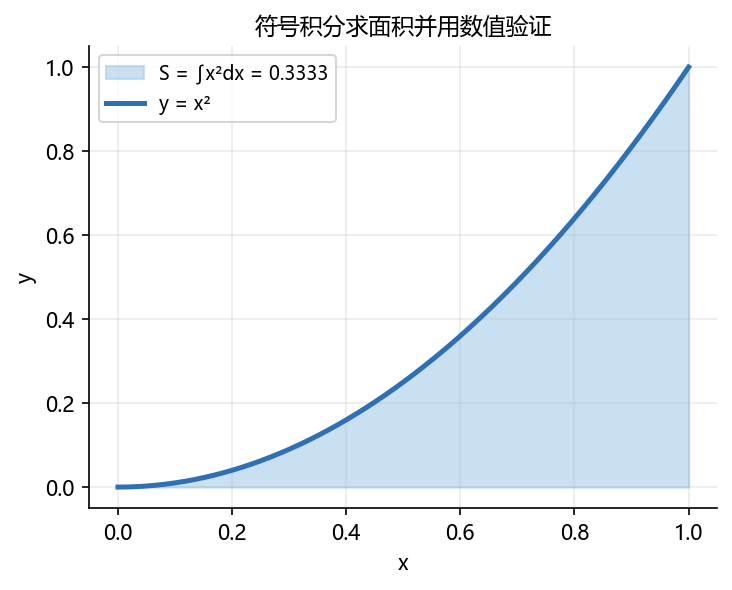
\includegraphics[keepaspectratio,alt={符号积分求面积}]{figures/02-sympy/sympy_area.png}}
\caption{符号积分求面积}
\end{figure}

\subsubsection{分析}\label{ux5206ux6790-2}

\begin{itemize}
\tightlist
\item
  SymPy 给出精确的 \(1/3\)，而 NumPy 的
  \texttt{np.trapz}/数值积分只能给出近似；
\item
  \texttt{sp.N(area)} 输出
  0.333333333333333，说明符号结果与数值结果一致；
\item
  这正体现``先符号推导得到公式，再数值计算/可视化''的方法论。
\end{itemize}

\subsubsection{拓展任务}\label{ux62d3ux5c55ux4efbux52a1-2}

\begin{enumerate}
\def\labelenumi{\arabic{enumi}.}
\tightlist
\item
  改求 \(y=e^{-x}\) 在 \([0,1]\) 上的面积，并与
  \texttt{scipy.integrate.quad} 比较；
\item
  求曲线 \(y=x^2\) 绕 \(x\)
  轴旋转一周的旋转体体积：\(\pi\int_0^1 x^4 dx\)，用 SymPy 验证；
\item
  把 \([0,1]\) 换成 \([a,b]\) 符号区间，观察 SymPy 是否保留符号结果。
\end{enumerate}

\begin{center}\rule{0.5\linewidth}{0.5pt}\end{center}

\subsection{案例 2：符号导数 → 切线方程 →
数值验证}\label{ux6848ux4f8b-2ux7b26ux53f7ux5bfcux6570-ux5207ux7ebfux65b9ux7a0b-ux6570ux503cux9a8cux8bc1}

\subsubsection{背景}\label{ux80ccux666f-3}

求 \(y=\sin x\) 在 \(x=1\) 处的切线方程。先用 SymPy 求导得到
\(\cos x\)，再求斜率 \(\cos(1)\)，最后用 \texttt{lambdify}
画图，并与数值差商验证。

\subsubsection{代码}\label{ux4ee3ux7801-2}

\begin{Shaded}
\begin{Highlighting}[]
\ImportTok{import}\NormalTok{ sympy }\ImportTok{as}\NormalTok{ sp}
\ImportTok{import}\NormalTok{ numpy }\ImportTok{as}\NormalTok{ np}
\NormalTok{x }\OperatorTok{=}\NormalTok{ sp.symbols(}\StringTok{\textquotesingle{}x\textquotesingle{}}\NormalTok{)}
\NormalTok{f }\OperatorTok{=}\NormalTok{ sp.sin(x)}
\NormalTok{df }\OperatorTok{=}\NormalTok{ sp.diff(f, x)}
\BuiltInTok{print}\NormalTok{(df)   }\CommentTok{\# cos(x)}

\NormalTok{a }\OperatorTok{=} \DecValTok{1}
\NormalTok{slope }\OperatorTok{=}\NormalTok{ sp.N(df.subs(x, a))}
\BuiltInTok{print}\NormalTok{(slope)   }\CommentTok{\# cos(1) ≈ 0.540302305868140}

\NormalTok{tangent }\OperatorTok{=}\NormalTok{ sp.simplify(df.subs(x, a) }\OperatorTok{*}\NormalTok{ (x }\OperatorTok{{-}}\NormalTok{ a) }\OperatorTok{+}\NormalTok{ f.subs(x, a))}
\BuiltInTok{print}\NormalTok{(tangent)}

\CommentTok{\#\# 数值差商验证导数}
\NormalTok{h }\OperatorTok{=} \FloatTok{1e{-}6}
\NormalTok{numeric\_deriv }\OperatorTok{=}\NormalTok{ (sp.sin(a }\OperatorTok{+}\NormalTok{ h) }\OperatorTok{{-}}\NormalTok{ sp.sin(a }\OperatorTok{{-}}\NormalTok{ h)) }\OperatorTok{/}\NormalTok{ (}\DecValTok{2}\OperatorTok{*}\NormalTok{h)}
\BuiltInTok{print}\NormalTok{(}\BuiltInTok{float}\NormalTok{(sp.N(numeric\_deriv)))}
\end{Highlighting}
\end{Shaded}

\begin{Shaded}
\begin{Highlighting}[]
\NormalTok{cos(x)}
\NormalTok{0.540302305868140}
\NormalTok{(x {-} 1)*cos(1) + sin(1)}
\NormalTok{0.540302305840346}
\end{Highlighting}
\end{Shaded}

\subsubsection{可视化}\label{ux53efux89c6ux5316-1}

\begin{Shaded}
\begin{Highlighting}[]
\ImportTok{import}\NormalTok{ matplotlib.pyplot }\ImportTok{as}\NormalTok{ plt}

\NormalTok{plt.rcParams[}\StringTok{\textquotesingle{}font.sans{-}serif\textquotesingle{}}\NormalTok{] }\OperatorTok{=}\NormalTok{ [}\StringTok{\textquotesingle{}Microsoft YaHei\textquotesingle{}}\NormalTok{, }\StringTok{\textquotesingle{}SimHei\textquotesingle{}}\NormalTok{, }\StringTok{\textquotesingle{}DejaVu Sans\textquotesingle{}}\NormalTok{]}
\NormalTok{plt.rcParams[}\StringTok{\textquotesingle{}axes.unicode\_minus\textquotesingle{}}\NormalTok{] }\OperatorTok{=} \VariableTok{False}

\KeywordTok{def}\NormalTok{ tangent\_num(v):}
    \ControlFlowTok{return} \BuiltInTok{float}\NormalTok{(sp.N(tangent.subs(x, v)))}

\NormalTok{xn }\OperatorTok{=}\NormalTok{ np.linspace(}\OperatorTok{{-}}\DecValTok{1}\NormalTok{, }\DecValTok{3}\NormalTok{, }\DecValTok{400}\NormalTok{)}
\NormalTok{plt.figure(figsize}\OperatorTok{=}\NormalTok{(}\FloatTok{5.8}\NormalTok{, }\FloatTok{4.0}\NormalTok{))}
\NormalTok{plt.plot(xn, np.sin(xn), color}\OperatorTok{=}\StringTok{\textquotesingle{}\#2f6fb3\textquotesingle{}}\NormalTok{, lw}\OperatorTok{=}\FloatTok{2.4}\NormalTok{, label}\OperatorTok{=}\StringTok{\textquotesingle{}y = sin(x)\textquotesingle{}}\NormalTok{)}
\NormalTok{plt.plot(xn, [tangent\_num(v) }\ControlFlowTok{for}\NormalTok{ v }\KeywordTok{in}\NormalTok{ xn], color}\OperatorTok{=}\StringTok{\textquotesingle{}\#e07b39\textquotesingle{}}\NormalTok{, lw}\OperatorTok{=}\DecValTok{2}\NormalTok{, ls}\OperatorTok{=}\StringTok{\textquotesingle{}{-}{-}\textquotesingle{}}\NormalTok{,}
\NormalTok{         label}\OperatorTok{=}\SpecialStringTok{f\textquotesingle{}切线 (斜率 ≈ }\SpecialCharTok{\{}\BuiltInTok{float}\NormalTok{(slope)}\SpecialCharTok{:.4f\}}\SpecialStringTok{)\textquotesingle{}}\NormalTok{)}
\NormalTok{plt.plot([a], [np.sin(a)], }\StringTok{\textquotesingle{}o\textquotesingle{}}\NormalTok{, color}\OperatorTok{=}\StringTok{\textquotesingle{}\#c0392b\textquotesingle{}}\NormalTok{, ms}\OperatorTok{=}\DecValTok{7}\NormalTok{, label}\OperatorTok{=}\SpecialStringTok{f\textquotesingle{}切点 x=}\SpecialCharTok{\{}\NormalTok{a}\SpecialCharTok{\}}\SpecialStringTok{\textquotesingle{}}\NormalTok{)}
\NormalTok{plt.axhline(}\DecValTok{0}\NormalTok{, color}\OperatorTok{=}\StringTok{\textquotesingle{}\#666\textquotesingle{}}\NormalTok{, lw}\OperatorTok{=}\FloatTok{0.7}\NormalTok{)}\OperatorTok{;}\NormalTok{ plt.axvline(}\DecValTok{0}\NormalTok{, color}\OperatorTok{=}\StringTok{\textquotesingle{}\#666\textquotesingle{}}\NormalTok{, lw}\OperatorTok{=}\FloatTok{0.7}\NormalTok{)}
\NormalTok{plt.xlabel(}\StringTok{\textquotesingle{}x\textquotesingle{}}\NormalTok{)}\OperatorTok{;}\NormalTok{ plt.ylabel(}\StringTok{\textquotesingle{}y\textquotesingle{}}\NormalTok{)}
\NormalTok{plt.title(}\StringTok{\textquotesingle{}符号导数 → 切线方程\textquotesingle{}}\NormalTok{, fontsize}\OperatorTok{=}\DecValTok{11}\NormalTok{)}
\NormalTok{plt.legend()}\OperatorTok{;}\NormalTok{ plt.grid(alpha}\OperatorTok{=}\FloatTok{0.25}\NormalTok{)}
\NormalTok{plt.savefig(}\StringTok{\textquotesingle{}figures/02{-}sympy/sympy\_tangent.png\textquotesingle{}}\NormalTok{, bbox\_inches}\OperatorTok{=}\StringTok{\textquotesingle{}tight\textquotesingle{}}\NormalTok{)}
\NormalTok{plt.show()}
\end{Highlighting}
\end{Shaded}

\begin{figure}
\centering
\pandocbounded{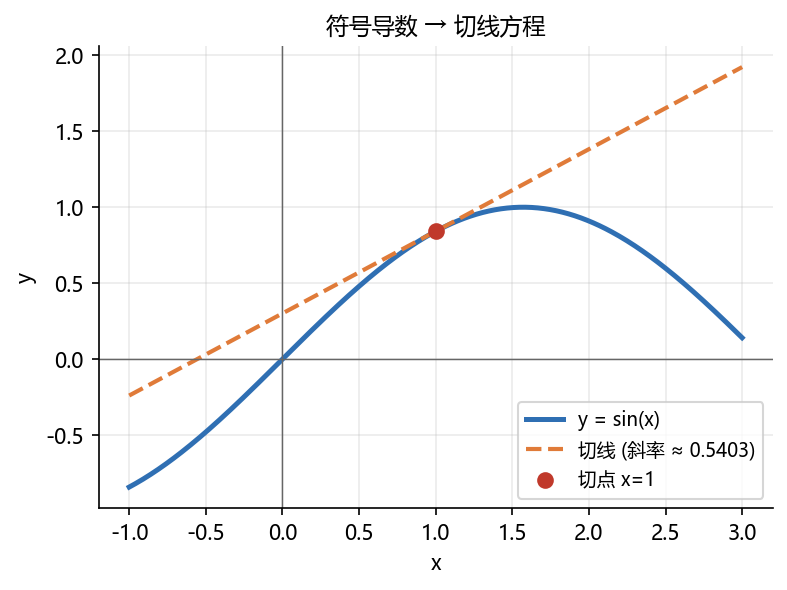
\includegraphics[keepaspectratio,alt={符号导数与切线}]{figures/02-sympy/sympy_tangent.png}}
\caption{符号导数与切线}
\end{figure}

\subsubsection{分析}\label{ux5206ux6790-3}

\begin{itemize}
\tightlist
\item
  符号求导得到 \(\cos x\)，代入 \(x=1\) 得斜率 ≈ 0.5403；
\item
  数值中心差商（\(h=10^{-6}\)）与符号导数一致，说明推导正确；
\item
  切线方程被 \texttt{simplify} 整理成
  \texttt{(x-1)*cos(1)\ +\ sin(1)}，可直接用于绘图/插值。
\end{itemize}

\subsubsection{拓展任务}\label{ux62d3ux5c55ux4efbux52a1-3}

\begin{enumerate}
\def\labelenumi{\arabic{enumi}.}
\tightlist
\item
  用 \texttt{lambdify} 把 \texttt{tangent} 和 \texttt{f}
  都转成数值函数，再比较在 \(x=0.5,1,1.5\) 处的数值；
\item
  求 \(y=\ln(x)\) 在 \(x=2\) 的法线方程并绘图；
\item
  把切线推广到二元函数（用梯度向量/切平面概念）。
\end{enumerate}

\begin{center}\rule{0.5\linewidth}{0.5pt}\end{center}

\subsection{案例
3：解方程并把根画在数轴上}\label{ux6848ux4f8b-3ux89e3ux65b9ux7a0bux5e76ux628aux6839ux753bux5728ux6570ux8f74ux4e0a}

\subsubsection{背景}\label{ux80ccux666f-4}

用 \texttt{solve} 求出多项式 \(x^2-5x+4=0\)
的根，并把函数曲线与根标注在同一张图上，直观理解``方程的解''就是``函数与
\(x\) 轴交点''。

\subsubsection{代码与输出}\label{ux4ee3ux7801ux4e0eux8f93ux51fa}

\begin{Shaded}
\begin{Highlighting}[]
\ImportTok{import}\NormalTok{ sympy }\ImportTok{as}\NormalTok{ sp}
\NormalTok{x }\OperatorTok{=}\NormalTok{ sp.symbols(}\StringTok{\textquotesingle{}x\textquotesingle{}}\NormalTok{)}
\NormalTok{p }\OperatorTok{=}\NormalTok{ x}\OperatorTok{**}\DecValTok{2} \OperatorTok{{-}} \DecValTok{5}\OperatorTok{*}\NormalTok{x }\OperatorTok{+} \DecValTok{4}
\NormalTok{roots }\OperatorTok{=} \BuiltInTok{sorted}\NormalTok{(sp.solve(p, x))}
\BuiltInTok{print}\NormalTok{(roots)}
\BuiltInTok{print}\NormalTok{([}\BuiltInTok{float}\NormalTok{(sp.N(r)) }\ControlFlowTok{for}\NormalTok{ r }\KeywordTok{in}\NormalTok{ roots])}
\end{Highlighting}
\end{Shaded}

\begin{Shaded}
\begin{Highlighting}[]
\NormalTok{[1, 4]}
\NormalTok{[1.0, 4.0]}
\end{Highlighting}
\end{Shaded}

\begin{figure}
\centering
\pandocbounded{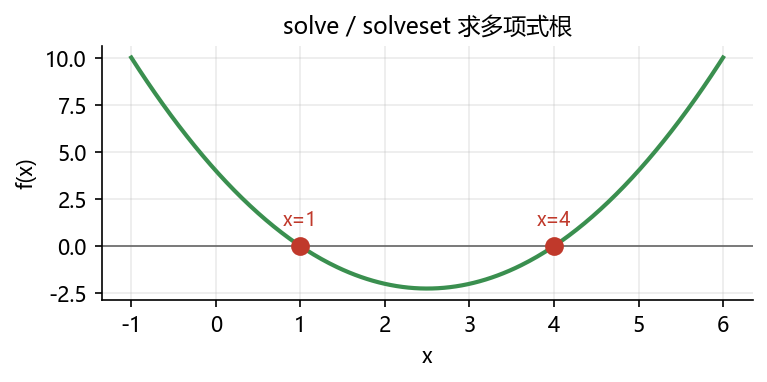
\includegraphics[keepaspectratio,alt={多项式根可视化}]{figures/02-sympy/sympy_roots.png}}
\caption{多项式根可视化}
\end{figure}

\subsubsection{分析}\label{ux5206ux6790-4}

\begin{itemize}
\tightlist
\item
  \texttt{solve} 精确返回整数根 1 和 4，无需浮点迭代；
\item
  根的位置与曲线穿越 \(x\)
  轴的位置一致，图片直观地体现``解方程=找零点''。
\end{itemize}

\subsubsection{拓展任务}\label{ux62d3ux5c55ux4efbux52a1-4}

\begin{enumerate}
\def\labelenumi{\arabic{enumi}.}
\tightlist
\item
  改求 \(x^3-6x^2+11x-6=0\) 的三个根并画图；
\item
  用 \texttt{solveset(...,\ domain=sp.S.Complexes)} 求解
  \(x^2+1=0\)，解释为什么实数域为空；
\item
  用 \texttt{lambdify} 把 \texttt{p} 转成数值函数，用 \texttt{np.roots}
  验证数值根。
\end{enumerate}

\subsection{本章综合练习（上机任务）}\label{ux672cux7ae0ux7efcux5408ux7ec3ux4e60ux4e0aux673aux4efbux52a1-1}

\begin{enumerate}
\def\labelenumi{\arabic{enumi}.}
\tightlist
\item
  用 SymPy 推导 \(y=\sqrt{x}\) 在 \([0,4]\) 上的面积，用 matplotlib
  绘制填充区域并标注精确值；
\item
  求 \(f(x)=x^3-3x\) 的极值点（提示：令 \(f'(x)=0\) 用
  \texttt{solve}），并画函数与极值点图；
\item
  把案例 1--3 整理成一个 \texttt{.ipynb}，写一份 200
  字以内的结论，说明``符号解 vs 数值解''各自的优势。
\end{enumerate}

\subsection{延伸阅读}\label{ux5ef6ux4f38ux9605ux8bfb-8}

\begin{itemize}
\tightlist
\item
  SymPy
  官方绘图（Plotting）模块：https://docs.sympy.org/latest/modules/plotting.html
\item
  Matplotlib
  填充区域：https://matplotlib.org/stable/api/\_as\_gen/matplotlib.pyplot.fill\_between.html
\item
  NumPy
  数值求根（np.roots）：https://numpy.org/doc/stable/reference/generated/numpy.roots.html
\end{itemize}

\section{04
常见误区与技巧}\label{ux5e38ux89c1ux8befux533aux4e0eux6280ux5de7-1}

\begin{quote}
本章为新增``查漏补缺''页：把学生最容易踩的坑集中列出，并给出正确的写法和性能技巧。
\end{quote}

\subsection{1.
高频误区速查表}\label{ux9ad8ux9891ux8befux533aux901fux67e5ux8868-1}

{\def\LTcaptype{none} % do not increment counter
\begin{longtable}[]{@{}
  >{\raggedright\arraybackslash}p{(\linewidth - 6\tabcolsep) * \real{0.2500}}
  >{\raggedright\arraybackslash}p{(\linewidth - 6\tabcolsep) * \real{0.2500}}
  >{\raggedright\arraybackslash}p{(\linewidth - 6\tabcolsep) * \real{0.2500}}
  >{\raggedright\arraybackslash}p{(\linewidth - 6\tabcolsep) * \real{0.2500}}@{}}
\toprule\noalign{}
\begin{minipage}[b]{\linewidth}\raggedright
\#
\end{minipage} & \begin{minipage}[b]{\linewidth}\raggedright
误区 / 错误写法
\end{minipage} & \begin{minipage}[b]{\linewidth}\raggedright
正确做法
\end{minipage} & \begin{minipage}[b]{\linewidth}\raggedright
原因
\end{minipage} \\
\midrule\noalign{}
\endhead
\bottomrule\noalign{}
\endlastfoot
1 & \texttt{pi\ =\ 3.14159} 然后参与符号运算 & 用 \texttt{sp.pi}（符号
π） & 浮点近似破坏精确性 \\
2 & \texttt{x\ +\ y\ ==\ y\ +\ x} 判断表达式相等 &
\texttt{sp.simplify((x+y)\ -\ (y+x))\ ==\ 0} 或
\texttt{(x+y).equals(y+x)} & \texttt{==} 比较的是结构不是数学等价 \\
3 & \texttt{sp.sqrt(x**2)} 期望得到 \texttt{x} &
\texttt{x\ =\ sp.Symbol(\textquotesingle{}x\textquotesingle{},\ positive=True)}
& 若无假设，\texttt{sqrt(x**2)=\textbar{}x\textbar{}} 更严谨 \\
4 & 用 \texttt{math.sin(x)} 而 \texttt{x} 是符号 & 用 \texttt{sp.sin(x)}
& \texttt{math} 只能处理浮点数 \\
5 & 以为 \texttt{lambdify} 返回符号表达式 &
它是数值函数，输入输出都是数值/数组 & 符号→数值的桥梁，不可再
\texttt{diff} \\
6 & \texttt{A\ *\ B} 想要 NumPy 式的逐元素乘 & SymPy \texttt{Matrix} 的
\texttt{*} 是矩阵乘；逐元素需 \texttt{sp.Matrix(A.applyfunc)} &
两种库的语义不同 \\
7 & \texttt{sp.solve(eq,\ x)} 忘记 \texttt{Eq} & 可以写
\texttt{sp.solve(eq,\ x)}（eq 视为=0）或
\texttt{sp.solve(sp.Eq(f,\ 0),\ x)} & 传入非 Eq 表达式默认等于 0 \\
8 & 用 \texttt{dsolve(eq)} 但没定义 \texttt{Function} &
\texttt{y\ =\ sp.Function(\textquotesingle{}y\textquotesingle{})(x)}；初值用
\texttt{ics=\{y.subs(x,0):\ 1\}} & 未定义函数会让 dsolve
报错/无法识别 \\
9 & 期望 \texttt{simplify} 万能 & 配合
\texttt{trigsimp}、\texttt{together}、\texttt{cancel}、\texttt{radsimp}
& 化简是启发式的 \\
10 & 用 \texttt{solve} 求所有复数根当实数用 & 用
\texttt{solveset(...,\ domain=sp.S.Reals)} 或 \texttt{real\_roots} &
不同求解函数返回集不同 \\
\end{longtable}
}

\subsection{2. 原理级难点：符号 vs
数值}\label{ux539fux7406ux7ea7ux96beux70b9ux7b26ux53f7-vs-ux6570ux503c}

\begin{Shaded}
\begin{Highlighting}[]
\ImportTok{import}\NormalTok{ sympy }\ImportTok{as}\NormalTok{ sp}
\NormalTok{x }\OperatorTok{=}\NormalTok{ sp.Symbol(}\StringTok{\textquotesingle{}x\textquotesingle{}}\NormalTok{)}
\NormalTok{expr }\OperatorTok{=}\NormalTok{ x}\OperatorTok{**}\DecValTok{2} \OperatorTok{+} \DecValTok{1}          \CommentTok{\# 符号表达式}
\BuiltInTok{print}\NormalTok{(}\BuiltInTok{type}\NormalTok{(expr))        }\CommentTok{\# \textless{}class \textquotesingle{}sympy.core.add.Add\textquotesingle{}\textgreater{}}

\NormalTok{val }\OperatorTok{=}\NormalTok{ expr.subs(x, }\DecValTok{2}\NormalTok{)    }\CommentTok{\# 仍是符号（整数 5）}
\BuiltInTok{print}\NormalTok{(val, }\BuiltInTok{type}\NormalTok{(val))}

\NormalTok{num }\OperatorTok{=}\NormalTok{ sp.N(expr.subs(x, }\DecValTok{2}\NormalTok{))   }\CommentTok{\# 数值}
\BuiltInTok{print}\NormalTok{(num, }\BuiltInTok{type}\NormalTok{(num))}

\NormalTok{f }\OperatorTok{=}\NormalTok{ sp.lambdify(x, expr, }\StringTok{\textquotesingle{}numpy\textquotesingle{}}\NormalTok{)}
\BuiltInTok{print}\NormalTok{(f(}\DecValTok{2}\NormalTok{))              }\CommentTok{\# 数值 5}
\end{Highlighting}
\end{Shaded}

要点：\textbf{符号对象}不参与浮点运算，只有
\texttt{subs}+\texttt{N}/\texttt{evalf} 或 \texttt{lambdify}
才会产生数值结果。

\subsection{3.
求解函数的选型}\label{ux6c42ux89e3ux51fdux6570ux7684ux9009ux578b}

{\def\LTcaptype{none} % do not increment counter
\begin{longtable}[]{@{}lll@{}}
\toprule\noalign{}
场景 & 推荐函数 & 说明 \\
\midrule\noalign{}
\endhead
\bottomrule\noalign{}
\endlastfoot
一元方程 & \texttt{solve} / \texttt{solveset} & \texttt{solveset}
更严谨 \\
线性方程组 & \texttt{linsolve} & 可传方程列表或 \texttt{(A,\ b)} \\
非线性方程组 & \texttt{nonlinsolve} / \texttt{solve} &
结果可能含复数解 \\
初等矩阵运算 & \texttt{Matrix} + 方法 &
\texttt{det}、\texttt{inv}、\texttt{eigenvals} \\
符号→数值 & \texttt{lambdify} & 指定
\texttt{\textquotesingle{}numpy\textquotesingle{}} \\
\end{longtable}
}

\subsection{4. 性能技巧}\label{ux6027ux80fdux6280ux5de7-1}

\begin{itemize}
\item
  \textbf{优先 \texttt{lambdify} 而不是逐点
  \texttt{subs}/\texttt{evalf}}：对大量数值点，先转成 NumPy
  函数再向量化计算，速度可提升百倍：

\begin{Shaded}
\begin{Highlighting}[]
\ImportTok{import}\NormalTok{ sympy }\ImportTok{as}\NormalTok{ sp, numpy }\ImportTok{as}\NormalTok{ np}
\NormalTok{x }\OperatorTok{=}\NormalTok{ sp.symbols(}\StringTok{\textquotesingle{}x\textquotesingle{}}\NormalTok{)}
\NormalTok{f }\OperatorTok{=}\NormalTok{ sp.lambdify(x, sp.sin(x)}\OperatorTok{/}\NormalTok{x, }\StringTok{\textquotesingle{}numpy\textquotesingle{}}\NormalTok{)}
\NormalTok{xs }\OperatorTok{=}\NormalTok{ np.linspace(}\FloatTok{0.001}\NormalTok{, }\DecValTok{10}\NormalTok{, }\DecValTok{100000}\NormalTok{)}
\NormalTok{ys }\OperatorTok{=}\NormalTok{ f(xs)          }\CommentTok{\# 一次向量化，比循环快得多}
\end{Highlighting}
\end{Shaded}
\item
  \textbf{\texttt{simplify} 要慎用}：可能很慢、甚至把结果变得更长；先试
  \texttt{cancel}/\texttt{together}/\texttt{trigsimp}；
\item
  \textbf{避免反复重建符号}：把符号与常用表达式定义一次，不要在循环里重复
  \texttt{symbols}；
\item
  \textbf{大矩阵用 \texttt{sp.Matrix} 的数值化}：若最终只需数值，考虑
  \texttt{sp.Matrix(...).evalf()} 或转成 NumPy \texttt{np.array(...)}
  再算；
\item
  \textbf{\texttt{nsimplify}
  做``反向''精确化}：把浮点近似还原为有理数/根式（如
  \texttt{sp.nsimplify(0.333333)} → \texttt{1/3}）。
\end{itemize}

\subsection{5. 调试建议}\label{ux8c03ux8bd5ux5efaux8bae-1}

\begin{enumerate}
\def\labelenumi{\arabic{enumi}.}
\tightlist
\item
  打印 \texttt{type(expr)}：确认是符号还是数值；
\item
  用 \texttt{sp.srepr(expr)} 查看底层树状结构，定位``为什么没化简''；
\item
  \texttt{expr.free\_symbols} 查看表达式含哪些符号；
\item
  \texttt{sp.solve} 无解时先试 \texttt{solveset}，再看 \texttt{domain}；
\item
  符号求导/积分结果可疑时，用数值验证：\texttt{sp.N(expr.subs(x,\ a))}
  与手工/数值结果对比；
\item
  复杂方程先 \texttt{sp.simplify} 或 \texttt{sp.expand} 再求。
\end{enumerate}

\subsection{6.
本章小结（自测）}\label{ux672cux7ae0ux5c0fux7ed3ux81eaux6d4b-1}

\begin{itemize}
\tightlist
\item[$\square$]
  能说明 \texttt{symbols} 与 \texttt{Symbol} 的区别；
\item[$\square$]
  能区分符号 π 与 \texttt{math.pi}；
\item[$\square$]
  能正确判断两个符号表达式是否数学等价；
\item[$\square$]
  能求极限、导数、积分并用数值验证；
\item[$\square$]
  能用
  \texttt{solve}/\texttt{solveset}/\texttt{linsolve}/\texttt{nonlinsolve}
  解对应问题；
\item[$\square$]
  会用 \texttt{lambdify} 把表达式转成数值函数；
\item[$\square$]
  会用 \texttt{dsolve} 解一/二阶微分方程并给定初值；
\item[$\square$]
  能用 \texttt{Matrix} 求特征值、雅可比矩阵。
\end{itemize}

\subsection{延伸阅读}\label{ux5ef6ux4f38ux9605ux8bfb-9}

\begin{itemize}
\tightlist
\item
  SymPy 官方 Tutorial：https://docs.sympy.org/latest/tutorial/index.html
\item
  SymPy 官方 FAQ：https://docs.sympy.org/latest/tutorial/gotchas.html
\item
  SymPy
  官方性能/数值化建议：https://docs.sympy.org/latest/modules/utilities/lambdify.html
\end{itemize}

\newpage

%% 由 build/emit_tex.py 生成（生成物，勿手改）；定制请放 user_style.tex / user_meta.yaml
\chapter{Scipy及其基本使用}\label{scipyux53caux5176ux57faux672cux4f7fux7528}

\section{01
微积分工具包：数值积分与微分方程数值解}\label{ux5faeux79efux5206ux5de5ux5177ux5305ux6570ux503cux79efux5206ux4e0eux5faeux5206ux65b9ux7a0bux6570ux503cux89e3}

\begin{quote}
本节对应原版 3.1 的内容，并增补学习目标、常见误区、思考题与延伸阅读。
所有代码均在 SciPy 1.15.2 / NumPy 2.1.2 环境实际运行验证。
配套图：\texttt{figures/03-scipy/ode\_solution.png}（由
\texttt{build/make\_chap3\_figures.py} 生成）。
\end{quote}

\subsection{本节目标}\label{ux672cux8282ux76eeux6807-6}

\begin{itemize}
\tightlist
\item
  会用手工梯形公式近似定积分，理解``分割越细越精确''的收敛思想；
\item
  会用 \texttt{scipy.integrate.quad} 求一维定积分，用
  \texttt{dblquad}/\texttt{nquad} 求多重积分；
\item
  会用 \texttt{trapezoid} 对离散数据（实验数据/数值解）做数值积分；
\item
  会用 \texttt{odeint}/\texttt{solve\_ivp}
  求解一阶、高阶及常微分方程组；
\item
  了解 \texttt{solve\_bvp} 用于边值问题。
\end{itemize}

\subsection{先修}\label{ux5148ux4fee-6}

\begin{itemize}
\tightlist
\item
  第 1 章 NumPy：\texttt{np.linspace}、\texttt{np.arange}、数组切片；
\item
  第 2 章 SymPy：知道解析积分与数值积分的区别（可先跳过）。
\end{itemize}

\subsection{官方文档 /
参考入口}\label{ux5b98ux65b9ux6587ux6863-ux53c2ux8003ux5165ux53e3}

\begin{itemize}
\tightlist
\item
  SciPy
  积分模块总览：https://docs.scipy.org/doc/scipy/reference/integrate.html
\item
  \texttt{quad}：https://docs.scipy.org/doc/scipy/reference/generated/scipy.integrate.quad.html
\item
  \texttt{solve\_ivp}：https://docs.scipy.org/doc/scipy/reference/generated/scipy.integrate.solve\_ivp.html
\end{itemize}

\begin{center}\rule{0.5\linewidth}{0.5pt}\end{center}

\subsection{1.1
为什么需要数值积分}\label{ux4e3aux4ec0ux4e48ux9700ux8981ux6570ux503cux79efux5206}

很多函数的原函数无法写成初等函数（例如
\(e^{-x^2}\)、\(\sin(x^2)\)），或者我们只有离散的实验采样点。此时只能用数值方法求定积分。

\subsubsection{1.1.1
梯形法：从手工到库函数}\label{ux68afux5f62ux6cd5ux4eceux624bux5de5ux5230ux5e93ux51fdux6570}

把 \([a,b]\) 等分成 \(n\) 段，每段用梯形近似曲线下面积：

\[\int_a^b f(x)\,dx \approx \sum_{i=0}^{n-1}\frac{f(x_i)+f(x_{i+1})}{2}\cdot h,\quad h=\frac{b-a}{n}\]

下面用 Python 实现 \(\int_0^1 x^2 dx\)，理论值 \(\frac{1}{3}\)。

\begin{Shaded}
\begin{Highlighting}[]
\KeywordTok{def}\NormalTok{ trapezoidal\_rule(f, a, b, n):}
\NormalTok{    h }\OperatorTok{=}\NormalTok{ (b }\OperatorTok{{-}}\NormalTok{ a) }\OperatorTok{/}\NormalTok{ n}
\NormalTok{    s }\OperatorTok{=} \FloatTok{0.5} \OperatorTok{*}\NormalTok{ (f(a) }\OperatorTok{+}\NormalTok{ f(b))}
    \ControlFlowTok{for}\NormalTok{ i }\KeywordTok{in} \BuiltInTok{range}\NormalTok{(}\DecValTok{1}\NormalTok{, n):}
\NormalTok{        s }\OperatorTok{+=}\NormalTok{ f(a }\OperatorTok{+}\NormalTok{ i }\OperatorTok{*}\NormalTok{ h)}
    \ControlFlowTok{return}\NormalTok{ s }\OperatorTok{*}\NormalTok{ h}

\KeywordTok{def}\NormalTok{ f(x):}
    \ControlFlowTok{return}\NormalTok{ x}\OperatorTok{**}\DecValTok{2}

\ControlFlowTok{for}\NormalTok{ n }\KeywordTok{in}\NormalTok{ (}\DecValTok{10}\NormalTok{, }\DecValTok{100}\NormalTok{, }\DecValTok{1000}\NormalTok{):}
    \BuiltInTok{print}\NormalTok{(}\SpecialStringTok{f"n=}\SpecialCharTok{\{}\NormalTok{n}\SpecialCharTok{:5d\}}\SpecialStringTok{  approx=}\SpecialCharTok{\{}\NormalTok{trapezoidal\_rule(f, }\DecValTok{0}\NormalTok{, }\DecValTok{1}\NormalTok{, n)}\SpecialCharTok{:.10f\}}\SpecialStringTok{"}\NormalTok{)}
\BuiltInTok{print}\NormalTok{(}\StringTok{"theoretical = 1/3 ="}\NormalTok{, }\DecValTok{1}\OperatorTok{/}\DecValTok{3}\NormalTok{)}
\end{Highlighting}
\end{Shaded}

\begin{Shaded}
\begin{Highlighting}[]
\NormalTok{n=   10  approx=0.3350000000}
\NormalTok{n=  100  approx=0.3333500000}
\NormalTok{n= 1000  approx=0.3333335000}
\NormalTok{theoretical = 1/3 = 0.3333333333333333}
\end{Highlighting}
\end{Shaded}

可见 \(n\) 越大，结果越接近 \(\frac{1}{3}\)。

\subsubsection{\texorpdfstring{1.1.2 用 \texttt{quad}
求一维定积分}{1.1.2 用 quad 求一维定积分}}\label{ux7528-quad-ux6c42ux4e00ux7ef4ux5b9aux79efux5206}

\texttt{quad(func,\ a,\ b,\ args=...)} 返回二元组
\texttt{(积分值,\ 误差估计)}。它使用自适应算法，精度远高于固定步长的梯形法。

\begin{Shaded}
\begin{Highlighting}[]
\ImportTok{import}\NormalTok{ numpy }\ImportTok{as}\NormalTok{ np}
\ImportTok{from}\NormalTok{ scipy.integrate }\ImportTok{import}\NormalTok{ quad}
\BuiltInTok{print}\NormalTok{(quad(}\KeywordTok{lambda}\NormalTok{ x: x}\OperatorTok{**}\DecValTok{2}\NormalTok{, }\DecValTok{0}\NormalTok{, }\DecValTok{1}\NormalTok{))}
\BuiltInTok{print}\NormalTok{(quad(}\KeywordTok{lambda}\NormalTok{ x: np.exp(}\OperatorTok{{-}}\NormalTok{x}\OperatorTok{**}\DecValTok{2}\NormalTok{), }\OperatorTok{{-}}\NormalTok{np.inf, np.inf))}
\end{Highlighting}
\end{Shaded}

\begin{Shaded}
\begin{Highlighting}[]
\NormalTok{(0.33333333333333337, 3.700743415417189e{-}15)}
\NormalTok{(1.7724538509055159, 1.2386316961910534e{-}10)}
\end{Highlighting}
\end{Shaded}

第二个例子是高斯积分
\(\int_{-\infty}^{+\infty} e^{-x^2} dx = \sqrt{\pi}\approx1.77245\)，\texttt{quad}
也擅长处理无穷积分。

\subsubsection{\texorpdfstring{1.1.3 二重积分
\texttt{dblquad}}{1.1.3 二重积分 dblquad}}\label{ux4e8cux91cdux79efux5206-dblquad}

计算
\(\int_0^1\int_0^x x y\, dy\, dx\)。注意内层积分上下限函数以积分变量为自变量。

\begin{Shaded}
\begin{Highlighting}[]
\ImportTok{from}\NormalTok{ scipy.integrate }\ImportTok{import}\NormalTok{ dblquad}

\KeywordTok{def}\NormalTok{ f(y, x):}
    \ControlFlowTok{return}\NormalTok{ x }\OperatorTok{*}\NormalTok{ y}

\NormalTok{result, err }\OperatorTok{=}\NormalTok{ dblquad(f, }\DecValTok{0}\NormalTok{, }\DecValTok{1}\NormalTok{, }\KeywordTok{lambda}\NormalTok{ x: }\DecValTok{0}\NormalTok{, }\KeywordTok{lambda}\NormalTok{ x: x)}
\BuiltInTok{print}\NormalTok{(result, err)}
\end{Highlighting}
\end{Shaded}

\begin{Shaded}
\begin{Highlighting}[]
\NormalTok{0.125 5.515032205777789e{-}15}
\end{Highlighting}
\end{Shaded}

\begin{quote}
理论值 \(\frac{1}{8}\)；若积分变量更多，可用 \texttt{tplquad}（三重）或
\texttt{nquad}（任意维）。
\end{quote}

\subsubsection{\texorpdfstring{1.1.4 对离散数据积分
\texttt{trapezoid}}{1.1.4 对离散数据积分 trapezoid}}\label{ux5bf9ux79bbux6563ux6570ux636eux79efux5206-trapezoid}

实验数据只有采样点 \((x_i,y_i)\)，没有函数表达式，用
\texttt{trapezoid(y,\ x)}。注意：在 SciPy 1.15 中函数名为
\texttt{trapezoid}（老版本叫 \texttt{trapz}）。

\begin{Shaded}
\begin{Highlighting}[]
\ImportTok{from}\NormalTok{ scipy.integrate }\ImportTok{import}\NormalTok{ trapezoid}
\ImportTok{import}\NormalTok{ numpy }\ImportTok{as}\NormalTok{ np}

\NormalTok{x }\OperatorTok{=}\NormalTok{ np.linspace(}\DecValTok{0}\NormalTok{, }\DecValTok{1}\NormalTok{, }\DecValTok{100}\NormalTok{)}
\NormalTok{y }\OperatorTok{=}\NormalTok{ x}\OperatorTok{**}\DecValTok{2}
\BuiltInTok{print}\NormalTok{(trapezoid(y, x))}
\end{Highlighting}
\end{Shaded}

\begin{Shaded}
\begin{Highlighting}[]
\NormalTok{0.33335033840084355}
\end{Highlighting}
\end{Shaded}

\begin{center}\rule{0.5\linewidth}{0.5pt}\end{center}

\subsection{1.2
常微分方程数值解}\label{ux5e38ux5faeux5206ux65b9ux7a0bux6570ux503cux89e3}

大多数微分方程没有解析解，\texttt{scipy.integrate}
给出``列表法''近似解：针对自变量数组中的每个取值，给出高频精度的因变量值。

\subsubsection{\texorpdfstring{1.2.1 一阶
ODE：\texttt{odeint}}{1.2.1 一阶 ODE：odeint}}\label{ux4e00ux9636-odeodeint}

求 \(\frac{dy}{dt}=\sin(t^2)\)，\(y(0)=1\)。

\begin{Shaded}
\begin{Highlighting}[]
\ImportTok{import}\NormalTok{ numpy }\ImportTok{as}\NormalTok{ np}
\ImportTok{from}\NormalTok{ scipy.integrate }\ImportTok{import}\NormalTok{ odeint}

\KeywordTok{def}\NormalTok{ dy\_dt(y, t):}
    \ControlFlowTok{return}\NormalTok{ np.sin(t}\OperatorTok{**}\DecValTok{2}\NormalTok{)}

\NormalTok{y0 }\OperatorTok{=}\NormalTok{ [}\DecValTok{1}\NormalTok{]}
\NormalTok{t }\OperatorTok{=}\NormalTok{ np.arange(}\DecValTok{0}\NormalTok{, }\DecValTok{10}\NormalTok{, }\FloatTok{0.1}\NormalTok{)}
\NormalTok{y }\OperatorTok{=}\NormalTok{ odeint(dy\_dt, y0, t)}
\BuiltInTok{print}\NormalTok{(}\StringTok{"len ="}\NormalTok{, }\BuiltInTok{len}\NormalTok{(y), }\StringTok{"   y(0)="}\NormalTok{, y[}\DecValTok{0}\NormalTok{,}\DecValTok{0}\NormalTok{], }\StringTok{"   y(9.9)="}\NormalTok{, y[}\OperatorTok{{-}}\DecValTok{1}\NormalTok{,}\DecValTok{0}\NormalTok{])}
\end{Highlighting}
\end{Shaded}

\begin{Shaded}
\begin{Highlighting}[]
\NormalTok{len = 100   y(0)= 1.0   y(9.9)= 1.6678897279551907}
\end{Highlighting}
\end{Shaded}

\texttt{odeint} 默认 \texttt{func(y,\ t,\ *args)} 参数顺序（y 在前、t
在后），基于 LSODA 可自动处理刚性问题。

\subsubsection{1.2.2 二阶 ODE
转一阶方程组}\label{ux4e8cux9636-ode-ux8f6cux4e00ux9636ux65b9ux7a0bux7ec4}

求 \(y''+y=0\)，\(y(0)=1,\ y'(0)=0\)。令 \(y_1=y,\ y_2=y'\)，则
\(y_1'=y_2,\ y_2'=-y_1\)。

\begin{Shaded}
\begin{Highlighting}[]
\KeywordTok{def}\NormalTok{ second\_order(y, t):}
\NormalTok{    y1, y2 }\OperatorTok{=}\NormalTok{ y}
    \ControlFlowTok{return}\NormalTok{ [y2, }\OperatorTok{{-}}\NormalTok{y1]}

\NormalTok{y }\OperatorTok{=}\NormalTok{ odeint(second\_order, [}\DecValTok{1}\NormalTok{, }\DecValTok{0}\NormalTok{], t)}
\BuiltInTok{print}\NormalTok{(}\StringTok{"y(9.9) ="}\NormalTok{, y[}\OperatorTok{{-}}\DecValTok{1}\NormalTok{,}\DecValTok{0}\NormalTok{], }\StringTok{"  y\textquotesingle{}(9.9) ="}\NormalTok{, y[}\OperatorTok{{-}}\DecValTok{1}\NormalTok{,}\DecValTok{1}\NormalTok{])}
\end{Highlighting}
\end{Shaded}

\begin{Shaded}
\begin{Highlighting}[]
\NormalTok{y(9.9) = {-}0.8891913778545403   y\textquotesingle{}(9.9) = 0.45753579354898755}
\end{Highlighting}
\end{Shaded}

\begin{quote}
该方程解析解为
\(y=\cos t\)，\(\cos(9.9)\approx -0.8892\)，\(y'(9.9)=-\sin(9.9)\approx 0.4575\)，数值解一致。
\end{quote}

\subsubsection{1.2.3 高阶
ODE：三阶方程}\label{ux9ad8ux9636-odeux4e09ux9636ux65b9ux7a0b}

对 \(y'''+y''+y'+y=0\)，令
\(y_1=y,\ y_2=y',\ y_3=y''\)，化为三个一阶方程：\(y_1'=y_2,\ y_2'=y_3,\ y_3'=-y_1-y_2-y_3\)。

\begin{Shaded}
\begin{Highlighting}[]
\KeywordTok{def}\NormalTok{ third\_order(y, t):}
\NormalTok{    y1, y2, y3 }\OperatorTok{=}\NormalTok{ y}
    \ControlFlowTok{return}\NormalTok{ [y2, y3, }\OperatorTok{{-}}\NormalTok{y1 }\OperatorTok{{-}}\NormalTok{ y2 }\OperatorTok{{-}}\NormalTok{ y3]}

\NormalTok{y }\OperatorTok{=}\NormalTok{ odeint(third\_order, [}\DecValTok{1}\NormalTok{, }\DecValTok{0}\NormalTok{, }\DecValTok{0}\NormalTok{], t)}
\BuiltInTok{print}\NormalTok{(}\StringTok{"y(9.9) ="}\NormalTok{, y[}\OperatorTok{{-}}\DecValTok{1}\NormalTok{,}\DecValTok{0}\NormalTok{], }\StringTok{"  y\textquotesingle{}(9.9) ="}\NormalTok{, y[}\OperatorTok{{-}}\DecValTok{1}\NormalTok{,}\DecValTok{1}\NormalTok{], }\StringTok{"  y\textquotesingle{}\textquotesingle{}(9.9) ="}\NormalTok{, y[}\OperatorTok{{-}}\DecValTok{1}\NormalTok{,}\DecValTok{2}\NormalTok{])}
\end{Highlighting}
\end{Shaded}

\begin{Shaded}
\begin{Highlighting}[]
\NormalTok{y(9.9) = {-}0.67333854   y\textquotesingle{}(9.9) = {-}0.21585283   y\textquotesingle{}\textquotesingle{}(9.9) = 0.67338872}
\end{Highlighting}
\end{Shaded}

\subsubsection{\texorpdfstring{1.2.4 更新更灵活的
\texttt{solve\_ivp}}{1.2.4 更新更灵活的 solve\_ivp}}\label{ux66f4ux65b0ux66f4ux7075ux6d3bux7684-solve_ivp}

\texttt{solve\_ivp} 是较新且更灵活的接口，支持
\texttt{t\_eval}、事件检测、更多求解器。注意它的导数函数签名是
\texttt{fun(t,\ y)}（t 在前）。

\begin{Shaded}
\begin{Highlighting}[]
\ImportTok{from}\NormalTok{ scipy.integrate }\ImportTok{import}\NormalTok{ solve\_ivp}

\KeywordTok{def}\NormalTok{ deriv(t, y):}
    \ControlFlowTok{return} \OperatorTok{{-}}\DecValTok{2} \OperatorTok{*}\NormalTok{ y}

\NormalTok{sol }\OperatorTok{=}\NormalTok{ solve\_ivp(deriv, (}\DecValTok{0}\NormalTok{, }\DecValTok{5}\NormalTok{), [}\DecValTok{1}\NormalTok{], t\_eval}\OperatorTok{=}\NormalTok{np.linspace(}\DecValTok{0}\NormalTok{, }\DecValTok{5}\NormalTok{, }\DecValTok{100}\NormalTok{))}
\BuiltInTok{print}\NormalTok{(}\StringTok{"y(5) ="}\NormalTok{, sol.y[}\DecValTok{0}\NormalTok{, }\OperatorTok{{-}}\DecValTok{1}\NormalTok{])}
\BuiltInTok{print}\NormalTok{(}\StringTok{"n\_points ="}\NormalTok{, }\BuiltInTok{len}\NormalTok{(sol.t))}
\end{Highlighting}
\end{Shaded}

\begin{Shaded}
\begin{Highlighting}[]
\NormalTok{y(5) = 4.572378941563548e{-}05}
\NormalTok{n\_points = 100}
\end{Highlighting}
\end{Shaded}

解析解 \(y=e^{-2t}\)，\(e^{-10}\approx4.54\times10^{-5}\)，数值解一致。

\subsubsection{\texorpdfstring{1.2.5 边值问题
\texttt{solve\_bvp}}{1.2.5 边值问题 solve\_bvp}}\label{ux8fb9ux503cux95eeux9898-solve_bvp}

边值问题（BVP）给定区间两端条件，且需要初始猜测。以下求 \(y''=6x\)，边界
\(y(0)=0,\ y(1)=1\)（解析解 \(y=x^3\)）。

\begin{Shaded}
\begin{Highlighting}[]
\ImportTok{from}\NormalTok{ scipy.integrate }\ImportTok{import}\NormalTok{ solve\_bvp}

\KeywordTok{def}\NormalTok{ fun(x, y):}
    \ControlFlowTok{return}\NormalTok{ np.vstack((y[}\DecValTok{1}\NormalTok{], }\DecValTok{6}\OperatorTok{*}\NormalTok{x))}

\KeywordTok{def}\NormalTok{ bc(ya, yb):}
    \ControlFlowTok{return}\NormalTok{ np.array([ya[}\DecValTok{0}\NormalTok{], yb[}\DecValTok{0}\NormalTok{]}\OperatorTok{{-}}\DecValTok{1}\NormalTok{])}

\NormalTok{x }\OperatorTok{=}\NormalTok{ np.linspace(}\DecValTok{0}\NormalTok{, }\DecValTok{1}\NormalTok{, }\DecValTok{20}\NormalTok{)}
\NormalTok{y }\OperatorTok{=}\NormalTok{ np.zeros((}\DecValTok{2}\NormalTok{, x.size))}
\NormalTok{sol }\OperatorTok{=}\NormalTok{ solve\_bvp(fun, bc, x, y)}
\BuiltInTok{print}\NormalTok{(}\StringTok{"sol.x.size ="}\NormalTok{, sol.x.size, }\StringTok{"   y\_mid ="}\NormalTok{, }\BuiltInTok{round}\NormalTok{(sol.y[}\DecValTok{0}\NormalTok{,}\DecValTok{10}\NormalTok{], }\DecValTok{6}\NormalTok{))}
\BuiltInTok{print}\NormalTok{(}\StringTok{"truth x\^{}3  ="}\NormalTok{, }\BuiltInTok{round}\NormalTok{(x[}\DecValTok{10}\NormalTok{]}\OperatorTok{**}\DecValTok{3}\NormalTok{, }\DecValTok{6}\NormalTok{))}
\end{Highlighting}
\end{Shaded}

\begin{Shaded}
\begin{Highlighting}[]
\NormalTok{sol.x.size = 20   y\_mid = 0.145794}
\NormalTok{truth x\^{}3  = 0.145794}
\end{Highlighting}
\end{Shaded}

\begin{center}\rule{0.5\linewidth}{0.5pt}\end{center}

\subsection{常见误区}\label{ux5e38ux89c1ux8befux533a-6}

\begin{enumerate}
\def\labelenumi{\arabic{enumi}.}
\tightlist
\item
  \textbf{\texttt{trapz} 在新版 SciPy 已改名}：用
  \texttt{trapezoid}；老教程的
  \texttt{from\ scipy.integrate\ import\ trapz} 在 1.15 会报
  \texttt{ImportError}。
\item
  \textbf{\texttt{odeint} 导数函数参数顺序是 \texttt{(y,\ t)}}，而
  \texttt{solve\_ivp} 是 \texttt{(t,\ y)}，二者顺序相反，容易写错。
\item
  \textbf{\texttt{solve\_ivp} 用 \texttt{t\_span=(t0,tf)}，不是
  \texttt{t0,tf} 分开传}；想要稀疏输出用 \texttt{t\_eval}。
\item
  \textbf{把 \texttt{quad} 返回元组当成单个值}：要取
  \texttt{quad(...){[}0{]}} 或解包 \texttt{(value,\ err)}。
\item
  \textbf{高阶 ODE 忘记降阶}：必须把
  \(y''\)（或更高阶）化成两个/多个一阶方程组成的方程组。
\item
  \textbf{\texttt{odeint} 时间序列必须单调}：\texttt{t}
  数组要递增或递减，且首项对应初始时间。
\end{enumerate}

\subsection{思考题}\label{ux601dux8003ux9898-6}

\begin{enumerate}
\def\labelenumi{\arabic{enumi}.}
\tightlist
\item
  为什么 \(n\) 增大时梯形法误差 \(O(h^2)\)，而 \texttt{quad}
  采用自适应细分能更快收敛？
\item
  用 \texttt{solve\_ivp} 重写 1.2.2 的二阶 ODE，并在
  \texttt{t=0,\ 2,\ 4,\ 9.9} 处与 \texttt{odeint} 结果对比。
\item
  说明 \texttt{solve\_ivp}
  的事件（\texttt{events}）可以解决什么问题（例如``何时达到给定阈值''）。
\end{enumerate}

\subsection{动手练习}\label{ux52a8ux624bux7ec3ux4e60}

\begin{itemize}
\tightlist
\item
  用 \texttt{trapezoid} 计算 \(\int_0^2 \sin(x)\,dx\)（理论值
  \(1-\cos2\)）；
\item
  用 \texttt{quad} 计算 \(\int_0^1 e^{-x^2}dx\)，并与 \texttt{trapezoid}
  的 n=1000 比较精度；
\item
  求解 SEIR 易感-暴露-感染-康复模型（参数见原版 3.1）并画出四条曲线；
\item
  用 \texttt{solve\_ivp} 求解 Lorenz 系统并画 3D 轨迹（参数
  \(\sigma=10,\rho=28,\beta=8/3\)）。
\end{itemize}

\subsection{延伸阅读}\label{ux5ef6ux4f38ux9605ux8bfb-10}

\begin{itemize}
\tightlist
\item
  SciPy 官方 ODE
  教程：https://docs.scipy.org/doc/scipy/reference/generated/scipy.integrate.solve\_ivp.html
\item
  SciPy
  积分教程：https://docs.scipy.org/doc/scipy/tutorial/integrate.html
\item
  数值积分/ODE
  的数学课件（中文）：https://docs.scipy.org.cn/doc/scipy/reference/integrate.html
\end{itemize}

\section{02
优化工具包：求根、极值、规划与曲线拟合}\label{ux4f18ux5316ux5de5ux5177ux5305ux6c42ux6839ux6781ux503cux89c4ux5212ux4e0eux66f2ux7ebfux62dfux5408}

\begin{quote}
本节对应原版 3.2 的内容，并增补学习目标、常见误区、思考题与延伸阅读。
所有代码均在 SciPy 1.15.2 / NumPy 2.1.2 环境实际运行验证。
配套图：\texttt{figures/03-scipy/optimize\_fit.png}（由
\texttt{build/make\_chap3\_figures.py} 生成）。
\end{quote}

\subsection{本节目标}\label{ux672cux8282ux76eeux6807-7}

\begin{itemize}
\tightlist
\item
  会用 \texttt{fsolve}/\texttt{root} 求非线性方程（组），用
  \texttt{brentq} 等一维求根；
\item
  会用
  \texttt{brent}（一维）、\texttt{fmin}（Nelder-Mead）、\texttt{minimize}（多种算法）求极值；
\item
  会用 \texttt{linprog} 解线性规划，用 \texttt{linear\_sum\_assignment}
  解指派问题；
\item
  会用 \texttt{leastsq}/\texttt{curve\_fit}
  做非线性最小二乘拟合，并读取协方差矩阵 \texttt{pcov}；
\item
  理解``初值敏感''与``约束处理''对数值优化的影响。
\end{itemize}

\subsection{先修}\label{ux5148ux4fee-7}

\begin{itemize}
\tightlist
\item
  第 1 章 NumPy：数组运算、随机数生成、\texttt{np.linalg}；
\item
  微积分求导/偏导概念；第 2 章 SymPy 可辅助写目标函数。
\end{itemize}

\subsection{官方文档 /
参考入口}\label{ux5b98ux65b9ux6587ux6863-ux53c2ux8003ux5165ux53e3-1}

\begin{itemize}
\tightlist
\item
  SciPy
  优化模块总览：https://docs.scipy.org/doc/scipy/reference/optimize.html
\item
  \texttt{root}：https://docs.scipy.org/doc/scipy/reference/generated/scipy.optimize.root.html
\item
  \texttt{minimize}：https://docs.scipy.org/doc/scipy/reference/generated/scipy.optimize.minimize.html
\item
  \texttt{curve\_fit}：https://docs.scipy.org/doc/scipy/reference/generated/scipy.optimize.curve\_fit.html
\end{itemize}

\begin{center}\rule{0.5\linewidth}{0.5pt}\end{center}

\subsection{2.1
函数的零点与方程的解}\label{ux51fdux6570ux7684ux96f6ux70b9ux4e0eux65b9ux7a0bux7684ux89e3}

\subsubsection{\texorpdfstring{2.1.1
\texttt{fsolve}：求单个方程/方程组的根}{2.1.1 fsolve：求单个方程/方程组的根}}\label{fsolveux6c42ux5355ux4e2aux65b9ux7a0bux65b9ux7a0bux7ec4ux7684ux6839}

求 \(x^2-612=0\) 的正根。\texttt{fsolve} 用最小二乘（典型
Levenberg-Marquardt）从初值出发迭代。

\begin{Shaded}
\begin{Highlighting}[]
\ImportTok{from}\NormalTok{ scipy.optimize }\ImportTok{import}\NormalTok{ fsolve}

\KeywordTok{def}\NormalTok{ func(x):}
    \ControlFlowTok{return}\NormalTok{ x}\OperatorTok{**}\DecValTok{2} \OperatorTok{{-}} \DecValTok{612}

\BuiltInTok{print}\NormalTok{(fsolve(func, }\FloatTok{10.0}\NormalTok{))}
\end{Highlighting}
\end{Shaded}

\begin{Shaded}
\begin{Highlighting}[]
\NormalTok{[24.73863375]}
\end{Highlighting}
\end{Shaded}

注意：\texttt{\$\textbackslash{}sqrt\{612\}\textbackslash{}approx24.7386\$}；若从
\texttt{-10} 出发会得到负根。\texttt{fsolve}
的结果依赖初值，且可能只找到最接近初值的一个根。

\subsubsection{\texorpdfstring{2.1.2
\texttt{root}：更多算法与方程组}{2.1.2 root：更多算法与方程组}}\label{rootux66f4ux591aux7b97ux6cd5ux4e0eux65b9ux7a0bux7ec4}

求方程组 \(\begin{cases}x^2+y^2-4=0\\ x-y-1=0\end{cases}\)。

\begin{Shaded}
\begin{Highlighting}[]
\ImportTok{from}\NormalTok{ scipy.optimize }\ImportTok{import}\NormalTok{ root}
\ImportTok{import}\NormalTok{ numpy }\ImportTok{as}\NormalTok{ np}

\KeywordTok{def}\NormalTok{ func(v):}
\NormalTok{    x, y }\OperatorTok{=}\NormalTok{ v}
    \ControlFlowTok{return}\NormalTok{ [x}\OperatorTok{**}\DecValTok{2} \OperatorTok{+}\NormalTok{ y}\OperatorTok{**}\DecValTok{2} \OperatorTok{{-}} \DecValTok{4}\NormalTok{, x }\OperatorTok{{-}}\NormalTok{ y }\OperatorTok{{-}} \DecValTok{1}\NormalTok{]}

\NormalTok{sol }\OperatorTok{=}\NormalTok{ root(func, [}\DecValTok{0}\NormalTok{, }\DecValTok{0}\NormalTok{])}
\BuiltInTok{print}\NormalTok{(sol.x, sol.success, sol.message)}
\end{Highlighting}
\end{Shaded}

\begin{Shaded}
\begin{Highlighting}[]
\NormalTok{[{-}0.82287566 {-}1.82287566] True The solution converged.}
\end{Highlighting}
\end{Shaded}

\texttt{root} 返回 \texttt{OptimizeResult}：\texttt{x}
为解，\texttt{success} 是否成功，\texttt{message} 终止信息，也可用
\texttt{method} 选择 \texttt{hybr}/\texttt{lm}/\texttt{krylov} 等。

\subsubsection{\texorpdfstring{2.1.3 一维求根
\texttt{brentq}}{2.1.3 一维求根 brentq}}\label{ux4e00ux7ef4ux6c42ux6839-brentq}

\texttt{brentq} 需要提供包含根的区间 \([a,b]\)，要求 \(f(a)\) 与
\(f(b)\) 异号。求 \(x^2-2=0\) 的根（\(\sqrt2\)）。

\begin{Shaded}
\begin{Highlighting}[]
\ImportTok{from}\NormalTok{ scipy.optimize }\ImportTok{import}\NormalTok{ brentq}
\BuiltInTok{print}\NormalTok{(brentq(}\KeywordTok{lambda}\NormalTok{ x: x}\OperatorTok{**}\DecValTok{2} \OperatorTok{{-}} \DecValTok{2}\NormalTok{, }\DecValTok{1}\NormalTok{, }\DecValTok{2}\NormalTok{))}
\end{Highlighting}
\end{Shaded}

\begin{Shaded}
\begin{Highlighting}[]
\NormalTok{1.4142135623731364}
\end{Highlighting}
\end{Shaded}

\begin{quote}
注意：\texttt{brent}（无 q）求的是\textbf{最小值}，\texttt{brentq}（带
q）求\textbf{根}，二者用途不同，切勿混淆。
\end{quote}

\subsection{2.2
函数的极值优化}\label{ux51fdux6570ux7684ux6781ux503cux4f18ux5316}

\subsubsection{\texorpdfstring{2.2.1
一维无约束：\texttt{brent}}{2.2.1 一维无约束：brent}}\label{ux4e00ux7ef4ux65e0ux7ea6ux675fbrent}

求 \(f(x)=(x-1)^2\) 的最小值点。

\begin{Shaded}
\begin{Highlighting}[]
\ImportTok{from}\NormalTok{ scipy.optimize }\ImportTok{import}\NormalTok{ brent}
\BuiltInTok{print}\NormalTok{(brent(}\KeywordTok{lambda}\NormalTok{ x: (x}\OperatorTok{{-}}\DecValTok{1}\NormalTok{)}\OperatorTok{**}\DecValTok{2}\NormalTok{, brack}\OperatorTok{=}\NormalTok{(}\DecValTok{0}\NormalTok{, }\DecValTok{2}\NormalTok{)))}
\end{Highlighting}
\end{Shaded}

\begin{Shaded}
\begin{Highlighting}[]
\NormalTok{0.9999999999999998}
\end{Highlighting}
\end{Shaded}

\texttt{brack} 是包含极小值的三点/两点区间。可设
\texttt{full\_output=True} 获得函数值、迭代次数等。

\subsubsection{\texorpdfstring{2.2.2
多维无约束：\texttt{fmin}（Nelder-Mead）}{2.2.2 多维无约束：fmin（Nelder-Mead）}}\label{ux591aux7ef4ux65e0ux7ea6ux675ffminnelder-mead}

求 \(f(x)=ax^2+bx+c\)，令 \(a=1,b=3,c=2\)。

\begin{Shaded}
\begin{Highlighting}[]
\ImportTok{from}\NormalTok{ scipy.optimize }\ImportTok{import}\NormalTok{ fmin}
\ImportTok{import}\NormalTok{ numpy }\ImportTok{as}\NormalTok{ np}

\KeywordTok{def}\NormalTok{ quadratic(x, a, b, c):}
    \ControlFlowTok{return}\NormalTok{ a }\OperatorTok{*}\NormalTok{ x}\OperatorTok{**}\DecValTok{2} \OperatorTok{+}\NormalTok{ b }\OperatorTok{*}\NormalTok{ x }\OperatorTok{+}\NormalTok{ c}

\NormalTok{res }\OperatorTok{=}\NormalTok{ fmin(quadratic, np.array([}\FloatTok{1.0}\NormalTok{]), args}\OperatorTok{=}\NormalTok{(}\DecValTok{1}\NormalTok{, }\DecValTok{3}\NormalTok{, }\DecValTok{2}\NormalTok{), full\_output}\OperatorTok{=}\VariableTok{True}\NormalTok{, disp}\OperatorTok{=}\VariableTok{False}\NormalTok{)}
\BuiltInTok{print}\NormalTok{(}\StringTok{"x ="}\NormalTok{, res[}\DecValTok{0}\NormalTok{], }\StringTok{"  fmin ="}\NormalTok{, res[}\DecValTok{1}\NormalTok{], }\StringTok{"  iter ="}\NormalTok{, res[}\DecValTok{2}\NormalTok{], }\StringTok{"  nfev ="}\NormalTok{, res[}\DecValTok{3}\NormalTok{])}
\end{Highlighting}
\end{Shaded}

\begin{Shaded}
\begin{Highlighting}[]
\NormalTok{x = [{-}1.5]   fmin = {-}0.25000000000000044   iter = 19   nfev = 38}
\end{Highlighting}
\end{Shaded}

理论最小点 \(x=-b/(2a)=-1.5\)，\(f_{\min}=c-b^2/(4a)=2-9/4=-0.25\)。

\subsubsection{\texorpdfstring{2.2.3 通用接口
\texttt{minimize}}{2.2.3 通用接口 minimize}}\label{ux901aux7528ux63a5ux53e3-minimize}

\texttt{minimize} 是更强大、更推荐的多维优化接口，可自动/手动选择算法。

\textbf{无约束}（Nelder-Mead）：

\begin{Shaded}
\begin{Highlighting}[]
\ImportTok{from}\NormalTok{ scipy.optimize }\ImportTok{import}\NormalTok{ minimize}

\KeywordTok{def}\NormalTok{ obj(x):}
    \ControlFlowTok{return}\NormalTok{ (x[}\DecValTok{0}\NormalTok{]}\OperatorTok{{-}}\DecValTok{1}\NormalTok{)}\OperatorTok{**}\DecValTok{2} \OperatorTok{+}\NormalTok{ (x[}\DecValTok{1}\NormalTok{]}\OperatorTok{{-}}\DecValTok{2}\NormalTok{)}\OperatorTok{**}\DecValTok{2}

\NormalTok{res }\OperatorTok{=}\NormalTok{ minimize(obj, [}\DecValTok{0}\NormalTok{, }\DecValTok{0}\NormalTok{], method}\OperatorTok{=}\StringTok{"Nelder{-}Mead"}\NormalTok{)}
\BuiltInTok{print}\NormalTok{(res.x, res.fun, res.success)}
\end{Highlighting}
\end{Shaded}

\begin{Shaded}
\begin{Highlighting}[]
\NormalTok{[0.99997307 2.00003382] 1.869184419935774e{-}09 True}
\end{Highlighting}
\end{Shaded}

\textbf{带约束}（SLSQP）：最小化 \(x_1^2+x_2^2\)，约束
\(x_1+x_2\ge1\)，\(x_1,x_2\ge0\)。

\begin{Shaded}
\begin{Highlighting}[]
\NormalTok{cons }\OperatorTok{=}\NormalTok{ [\{}\StringTok{"type"}\NormalTok{: }\StringTok{"ineq"}\NormalTok{, }\StringTok{"fun"}\NormalTok{: }\KeywordTok{lambda}\NormalTok{ x: x[}\DecValTok{0}\NormalTok{] }\OperatorTok{+}\NormalTok{ x[}\DecValTok{1}\NormalTok{] }\OperatorTok{{-}} \DecValTok{1}\NormalTok{\}]}
\NormalTok{res }\OperatorTok{=}\NormalTok{ minimize(}\KeywordTok{lambda}\NormalTok{ x: x[}\DecValTok{0}\NormalTok{]}\OperatorTok{**}\DecValTok{2} \OperatorTok{+}\NormalTok{ x[}\DecValTok{1}\NormalTok{]}\OperatorTok{**}\DecValTok{2}\NormalTok{, [}\DecValTok{0}\NormalTok{, }\DecValTok{0}\NormalTok{], method}\OperatorTok{=}\StringTok{"SLSQP"}\NormalTok{,}
\NormalTok{               constraints}\OperatorTok{=}\NormalTok{cons, bounds}\OperatorTok{=}\NormalTok{[(}\DecValTok{0}\NormalTok{, }\VariableTok{None}\NormalTok{), (}\DecValTok{0}\NormalTok{, }\VariableTok{None}\NormalTok{)])}
\BuiltInTok{print}\NormalTok{(res.x, res.fun, res.success)}
\end{Highlighting}
\end{Shaded}

\begin{Shaded}
\begin{Highlighting}[]
\NormalTok{[0.5 0.5] 0.5000000000000002 True}
\end{Highlighting}
\end{Shaded}

约束写成 \texttt{fun(x)\ \textgreater{}=\ 0} 形式；\texttt{bounds}
定义各变量取值范围。

\subsubsection{\texorpdfstring{2.2.4 线性规划
\texttt{linprog}}{2.2.4 线性规划 linprog}}\label{ux7ebfux6027ux89c4ux5212-linprog}

最小化 \(c^T x\)，受
\(A_{ub}x\le b_{ub}\)、\(A_{eq}x=b_{eq}\)、\(x\ge0\) 约束。

\begin{Shaded}
\begin{Highlighting}[]
\ImportTok{import}\NormalTok{ numpy }\ImportTok{as}\NormalTok{ np}
\ImportTok{from}\NormalTok{ scipy.optimize }\ImportTok{import}\NormalTok{ linprog}

\NormalTok{c }\OperatorTok{=}\NormalTok{ [}\OperatorTok{{-}}\DecValTok{29}\NormalTok{, }\OperatorTok{{-}}\DecValTok{45}\NormalTok{, }\DecValTok{0}\NormalTok{, }\DecValTok{0}\NormalTok{]}
\NormalTok{A\_ub }\OperatorTok{=}\NormalTok{ [[}\DecValTok{1}\NormalTok{, }\OperatorTok{{-}}\DecValTok{1}\NormalTok{, }\OperatorTok{{-}}\DecValTok{3}\NormalTok{, }\DecValTok{0}\NormalTok{], [}\OperatorTok{{-}}\DecValTok{2}\NormalTok{, }\DecValTok{3}\NormalTok{, }\DecValTok{7}\NormalTok{, }\OperatorTok{{-}}\DecValTok{3}\NormalTok{]]}
\NormalTok{b\_ub }\OperatorTok{=}\NormalTok{ [}\DecValTok{5}\NormalTok{, }\OperatorTok{{-}}\DecValTok{10}\NormalTok{]}
\NormalTok{A\_eq }\OperatorTok{=}\NormalTok{ [[}\DecValTok{2}\NormalTok{, }\DecValTok{8}\NormalTok{, }\DecValTok{1}\NormalTok{, }\DecValTok{0}\NormalTok{], [}\DecValTok{4}\NormalTok{, }\DecValTok{4}\NormalTok{, }\DecValTok{0}\NormalTok{, }\DecValTok{1}\NormalTok{]]}
\NormalTok{b\_eq }\OperatorTok{=}\NormalTok{ [}\DecValTok{60}\NormalTok{, }\DecValTok{60}\NormalTok{]}
\NormalTok{bounds }\OperatorTok{=}\NormalTok{ [(}\DecValTok{0}\NormalTok{, }\VariableTok{None}\NormalTok{)] }\OperatorTok{*} \DecValTok{4}

\NormalTok{res }\OperatorTok{=}\NormalTok{ linprog(c, A\_ub}\OperatorTok{=}\NormalTok{A\_ub, b\_ub}\OperatorTok{=}\NormalTok{b\_ub, A\_eq}\OperatorTok{=}\NormalTok{A\_eq, b\_eq}\OperatorTok{=}\NormalTok{b\_eq, bounds}\OperatorTok{=}\NormalTok{bounds)}
\BuiltInTok{print}\NormalTok{(np.}\BuiltInTok{round}\NormalTok{(res.x, }\DecValTok{2}\NormalTok{), }\BuiltInTok{round}\NormalTok{(res.fun, }\DecValTok{2}\NormalTok{), res.success)}
\end{Highlighting}
\end{Shaded}

\begin{Shaded}
\begin{Highlighting}[]
\NormalTok{[9.2 5.2 0.  2.4] {-}500.8 True}
\end{Highlighting}
\end{Shaded}

\subsubsection{\texorpdfstring{2.2.5 指派问题
\texttt{linear\_sum\_assignment}}{2.2.5 指派问题 linear\_sum\_assignment}}\label{ux6307ux6d3eux95eeux9898-linear_sum_assignment}

给定成本矩阵，求``一人一任务''的最小总成本分配（匈牙利算法）。

\begin{Shaded}
\begin{Highlighting}[]
\ImportTok{import}\NormalTok{ numpy }\ImportTok{as}\NormalTok{ np}
\ImportTok{from}\NormalTok{ scipy.optimize }\ImportTok{import}\NormalTok{ linear\_sum\_assignment}
\NormalTok{cost }\OperatorTok{=}\NormalTok{ [[}\DecValTok{4}\NormalTok{, }\DecValTok{1}\NormalTok{, }\DecValTok{3}\NormalTok{], [}\DecValTok{2}\NormalTok{, }\DecValTok{0}\NormalTok{, }\DecValTok{5}\NormalTok{], [}\DecValTok{3}\NormalTok{, }\DecValTok{2}\NormalTok{, }\DecValTok{2}\NormalTok{]]}
\NormalTok{row\_ind, col\_ind }\OperatorTok{=}\NormalTok{ linear\_sum\_assignment(cost)}
\BuiltInTok{print}\NormalTok{(}\StringTok{"rows ="}\NormalTok{, row\_ind, }\StringTok{"  cols ="}\NormalTok{, col\_ind)}
\BuiltInTok{print}\NormalTok{(}\StringTok{"min cost ="}\NormalTok{, np.array(cost)[row\_ind, col\_ind].}\BuiltInTok{sum}\NormalTok{())}
\end{Highlighting}
\end{Shaded}

\begin{Shaded}
\begin{Highlighting}[]
\NormalTok{rows = [0 1 2]   cols = [1 0 2]}
\NormalTok{min cost = 5}
\end{Highlighting}
\end{Shaded}

即工人 A→任务2、B→任务1、C→任务3，总成本 1+2+2=5。

\subsection{2.3
曲线拟合（最小二乘）}\label{ux66f2ux7ebfux62dfux5408ux6700ux5c0fux4e8cux4e58}

\subsubsection{\texorpdfstring{2.3.1
\texttt{leastsq}}{2.3.1 leastsq}}\label{leastsq}

手动给误差向量，最小化 \(\sum r_i^2\)。

\begin{Shaded}
\begin{Highlighting}[]
\ImportTok{import}\NormalTok{ numpy }\ImportTok{as}\NormalTok{ np}
\ImportTok{from}\NormalTok{ scipy.optimize }\ImportTok{import}\NormalTok{ leastsq}

\KeywordTok{def}\NormalTok{ model(x, a, b, c):}
    \ControlFlowTok{return}\NormalTok{ a}\OperatorTok{*}\NormalTok{x}\OperatorTok{**}\DecValTok{2} \OperatorTok{+}\NormalTok{ b}\OperatorTok{*}\NormalTok{x }\OperatorTok{+}\NormalTok{ c}

\KeywordTok{def}\NormalTok{ residuals(p, x, y):}
\NormalTok{    a, b, c }\OperatorTok{=}\NormalTok{ p}
    \ControlFlowTok{return}\NormalTok{ y }\OperatorTok{{-}}\NormalTok{ model(x, a, b, c)}

\NormalTok{rng }\OperatorTok{=}\NormalTok{ np.random.default\_rng(}\DecValTok{7}\NormalTok{)}
\NormalTok{x }\OperatorTok{=}\NormalTok{ np.linspace(}\OperatorTok{{-}}\DecValTok{10}\NormalTok{, }\DecValTok{10}\NormalTok{, }\DecValTok{50}\NormalTok{)}
\NormalTok{y }\OperatorTok{=}\NormalTok{ model(x, }\DecValTok{2}\NormalTok{, }\DecValTok{3}\NormalTok{, }\DecValTok{1}\NormalTok{) }\OperatorTok{+}\NormalTok{ rng.normal(}\DecValTok{0}\NormalTok{, }\DecValTok{2}\NormalTok{, }\BuiltInTok{len}\NormalTok{(x))}

\NormalTok{params, flag }\OperatorTok{=}\NormalTok{ leastsq(residuals, [}\DecValTok{0}\NormalTok{, }\DecValTok{0}\NormalTok{, }\DecValTok{0}\NormalTok{], args}\OperatorTok{=}\NormalTok{(x, y))}
\BuiltInTok{print}\NormalTok{(np.}\BuiltInTok{round}\NormalTok{(params, }\DecValTok{4}\NormalTok{))}
\end{Highlighting}
\end{Shaded}

\begin{Shaded}
\begin{Highlighting}[]
\NormalTok{[ 2.0191  3.0387 {-}0.2494]}
\end{Highlighting}
\end{Shaded}

\subsubsection{\texorpdfstring{2.3.2 更友好的
\texttt{curve\_fit}}{2.3.2 更友好的 curve\_fit}}\label{ux66f4ux53cbux597dux7684-curve_fit}

\texttt{curve\_fit(model,\ xdata,\ ydata,\ p0=...)} 自动构造残差，返回
\texttt{(popt,\ pcov)}。

\begin{Shaded}
\begin{Highlighting}[]
\ImportTok{import}\NormalTok{ numpy }\ImportTok{as}\NormalTok{ np}
\ImportTok{from}\NormalTok{ scipy.optimize }\ImportTok{import}\NormalTok{ curve\_fit}
\NormalTok{popt, pcov }\OperatorTok{=}\NormalTok{ curve\_fit(model, x, y, p0}\OperatorTok{=}\NormalTok{[}\DecValTok{0}\NormalTok{, }\DecValTok{0}\NormalTok{, }\DecValTok{0}\NormalTok{])}
\NormalTok{perr }\OperatorTok{=}\NormalTok{ np.sqrt(np.diag(pcov))}
\BuiltInTok{print}\NormalTok{(}\StringTok{"popt ="}\NormalTok{, np.}\BuiltInTok{round}\NormalTok{(popt, }\DecValTok{4}\NormalTok{))}
\BuiltInTok{print}\NormalTok{(}\StringTok{"stderr ="}\NormalTok{, np.}\BuiltInTok{round}\NormalTok{(perr, }\DecValTok{4}\NormalTok{))}
\end{Highlighting}
\end{Shaded}

\begin{Shaded}
\begin{Highlighting}[]
\NormalTok{popt = [ 2.0191  3.0387 {-}0.2494]}
\NormalTok{stderr = [0.0078 0.0409 0.3616]}
\end{Highlighting}
\end{Shaded}

真实参数为 \((2,3,1)\)，拟合值在其附近；\texttt{pcov}
对角线开方可作参数标准误的近似。

\begin{center}\rule{0.5\linewidth}{0.5pt}\end{center}

\subsection{常见误区}\label{ux5e38ux89c1ux8befux533a-7}

{\def\LTcaptype{none} % do not increment counter
\begin{longtable}[]{@{}
  >{\raggedright\arraybackslash}p{(\linewidth - 4\tabcolsep) * \real{0.3333}}
  >{\raggedright\arraybackslash}p{(\linewidth - 4\tabcolsep) * \real{0.3333}}
  >{\raggedright\arraybackslash}p{(\linewidth - 4\tabcolsep) * \real{0.3333}}@{}}
\toprule\noalign{}
\begin{minipage}[b]{\linewidth}\raggedright
\#
\end{minipage} & \begin{minipage}[b]{\linewidth}\raggedright
误区
\end{minipage} & \begin{minipage}[b]{\linewidth}\raggedright
正确做法
\end{minipage} \\
\midrule\noalign{}
\endhead
\bottomrule\noalign{}
\endlastfoot
1 & 用 \texttt{brent} 求根 & 求根用
\texttt{brentq}/\texttt{fsolve}/\texttt{root} \\
2 & \texttt{fsolve} 不设初值 / 期望得到全部根 & 一维用 \texttt{brentq}
且给出异号区间；多根问题改变初值或多个区间 \\
3 & \texttt{fmin} 的 \texttt{full\_output} 返回顺序误读 & 返回
\texttt{(xopt,\ fopt,\ iter,\ funcalls,\ ...)}，\texttt{iter}/\texttt{funcalls}
是整数 \\
4 & \texttt{linprog} 目标默认最小化，忘了 \texttt{c} 取负号 &
若原问题是最大化，把 \texttt{c} 取负转成最小化 \\
5 & \texttt{linear\_sum\_assignment} 直接返回成本矩阵 & 返回
\texttt{row\_ind,\ col\_ind}，需用
\texttt{cost{[}row\_ind,\ col\_ind{]}.sum()} 得成本 \\
6 & \texttt{minimize} 约束符号写反 & \texttt{ineq} 表示
\texttt{fun(x)\ \textgreater{}=\ 0}；等号约束用 \texttt{eq} \\
7 & 不设 \texttt{p0} 就 \texttt{curve\_fit} &
初值不良会导致不收敛或收敛到错误参数，应给接近真实值的 \texttt{p0} \\
\end{longtable}
}

\subsection{思考题}\label{ux601dux8003ux9898-7}

\begin{enumerate}
\def\labelenumi{\arabic{enumi}.}
\tightlist
\item
  为什么 \texttt{brentq} 比 \texttt{fsolve}
  在一维问题上更稳定？各需要什么前提？
\item
  \texttt{minimize} 的 \texttt{BFGS} 与 \texttt{Nelder-Mead}
  各适合什么情况？带约束时为何常用 \texttt{SLSQP}？
\item
  \texttt{curve\_fit} 的 \texttt{pcov}
  能给出参数标准误，但什么条件下这种近似才成立？
\end{enumerate}

\subsection{动手练习}\label{ux52a8ux624bux7ec3ux4e60-1}

\begin{itemize}
\tightlist
\item
  求 \(x^3-x-1=0\) 在 \([1,2]\) 内的根（用 \texttt{brentq} 与
  \texttt{fsolve}）；
\item
  用 \texttt{minimize} 求 Rosenbrock 函数
  \(f(x,y)=(1-x)^2+100(y-x^2)^2\) 的最小值（初值 \((-1.2,1)\)）；
\item
  用 \texttt{linprog} 解一个含 3 个变量、2 个不等式约束的小规划；
\item
  给一组 \((x,y)\) 数据，比较 \texttt{leastsq} 与 \texttt{curve\_fit}
  拟合一次线性函数 \(y=ax+b\) 的结果。
\end{itemize}

\subsection{延伸阅读}\label{ux5ef6ux4f38ux9605ux8bfb-11}

\begin{itemize}
\tightlist
\item
  SciPy
  推荐拟合教程：https://scipy.github.io/old-wiki/pages/Cookbook/OptimizationAndFitDemo1.html
\item
  \texttt{minimize}
  各方法说明：https://docs.scipy.org/doc/scipy/reference/generated/scipy.optimize.minimize.html
\item
  scikit-learn / statsmodels
  中的回归（后续章节会用到）：https://www.statsmodels.org/stable/regression.html
\end{itemize}

\section{03
插值工具包：一维/多维插值与样条}\label{ux63d2ux503cux5de5ux5177ux5305ux4e00ux7ef4ux591aux7ef4ux63d2ux503cux4e0eux6837ux6761}

\begin{quote}
本节对应原版 3.3 的内容，并增补学习目标、常见误区、思考题与延伸阅读。
所有代码均在 SciPy 1.15.2 / NumPy 2.1.2 环境实际运行验证。
配套图：\texttt{figures/03-scipy/interp\_compare.png}（由
\texttt{build/make\_chap3\_figures.py} 生成）。
\end{quote}

\subsection{本节目标}\label{ux672cux8282ux76eeux6807-8}

\begin{itemize}
\tightlist
\item
  理解插值（interpolation）与拟合（fitting）的区别；
\item
  会用 \texttt{CubicSpline}、一维 \texttt{interp1d} 做一维插值；
\item
  会用 \texttt{RegularGridInterpolator} 做规则网格上的多维插值；
\item
  会用 \texttt{griddata} 对散点数据做插值并可视化；
\item
  了解线性插值、样条插值的优劣与龙格现象。
\end{itemize}

\subsection{先修}\label{ux5148ux4fee-8}

\begin{itemize}
\tightlist
\item
  第 1 章
  NumPy：\texttt{meshgrid}、\texttt{flatten}、\texttt{reshape}、随机数；
\item
  Matplotlib 基础（\texttt{contourf}/\texttt{scatter} 可选）。
\end{itemize}

\subsection{官方文档 /
参考入口}\label{ux5b98ux65b9ux6587ux6863-ux53c2ux8003ux5165ux53e3-2}

\begin{itemize}
\tightlist
\item
  SciPy
  插值模块总览：https://docs.scipy.org/doc/scipy/reference/interpolate.html
\item
  \texttt{CubicSpline}：https://docs.scipy.org/doc/scipy/reference/generated/scipy.interpolate.CubicSpline.html
\item
  \texttt{RegularGridInterpolator}：https://docs.scipy.org/doc/scipy/reference/generated/scipy.interpolate.RegularGridInterpolator.html
\item
  \texttt{griddata}：https://docs.scipy.org/doc/scipy/reference/generated/scipy.interpolate.griddata.html
\end{itemize}

\begin{center}\rule{0.5\linewidth}{0.5pt}\end{center}

\subsection{3.1 一维插值}\label{ux4e00ux7ef4ux63d2ux503c}

已知 \(n\) 个点 \((x_i,y_i)\)，要在 \(x\) 的任意位置估计
\(y\)。线性插值用直线连接数据点；三次样条用分段三次多项式，保证一阶/二阶导数连续，曲线更光滑。

\subsubsection{\texorpdfstring{3.1.1 使用
\texttt{np.interp}（线性）}{3.1.1 使用 np.interp（线性）}}\label{ux4f7fux7528-np.interpux7ebfux6027}

\begin{Shaded}
\begin{Highlighting}[]
\ImportTok{import}\NormalTok{ numpy }\ImportTok{as}\NormalTok{ np}
\NormalTok{x }\OperatorTok{=}\NormalTok{ np.array([}\DecValTok{0}\NormalTok{, }\DecValTok{1}\NormalTok{, }\DecValTok{2}\NormalTok{, }\DecValTok{3}\NormalTok{, }\DecValTok{4}\NormalTok{, }\DecValTok{5}\NormalTok{])}
\NormalTok{y }\OperatorTok{=}\NormalTok{ np.array([}\DecValTok{0}\NormalTok{, }\FloatTok{0.8}\NormalTok{, }\FloatTok{0.9}\NormalTok{, }\FloatTok{0.1}\NormalTok{, }\OperatorTok{{-}}\FloatTok{0.8}\NormalTok{, }\OperatorTok{{-}}\DecValTok{1}\NormalTok{])}
\BuiltInTok{print}\NormalTok{(np.interp([}\FloatTok{0.5}\NormalTok{, }\FloatTok{2.5}\NormalTok{, }\FloatTok{4.5}\NormalTok{], x, y))}
\end{Highlighting}
\end{Shaded}

\begin{Shaded}
\begin{Highlighting}[]
\NormalTok{[ 0.4  0.5 {-}0.9]}
\end{Highlighting}
\end{Shaded}

\texttt{np.interp} 只能用线性插值，速度最快。

\subsubsection{\texorpdfstring{3.1.2 经典的
\texttt{interp1d}（注意：新版本建议优先
\texttt{CubicSpline}）}{3.1.2 经典的 interp1d（注意：新版本建议优先 CubicSpline）}}\label{ux7ecfux5178ux7684-interp1dux6ce8ux610fux65b0ux7248ux672cux5efaux8baeux4f18ux5148-cubicspline}

\begin{Shaded}
\begin{Highlighting}[]
\ImportTok{from}\NormalTok{ scipy.interpolate }\ImportTok{import}\NormalTok{ interp1d}
\NormalTok{f\_lin }\OperatorTok{=}\NormalTok{ interp1d(x, y, kind}\OperatorTok{=}\StringTok{"linear"}\NormalTok{)}
\NormalTok{f\_cub }\OperatorTok{=}\NormalTok{ interp1d(x, y, kind}\OperatorTok{=}\StringTok{"cubic"}\NormalTok{)}
\BuiltInTok{print}\NormalTok{(np.}\BuiltInTok{round}\NormalTok{(f\_lin([}\FloatTok{0.5}\NormalTok{, }\FloatTok{2.5}\NormalTok{, }\FloatTok{4.5}\NormalTok{]), }\DecValTok{4}\NormalTok{))}
\BuiltInTok{print}\NormalTok{(np.}\BuiltInTok{round}\NormalTok{(f\_cub([}\FloatTok{0.5}\NormalTok{, }\FloatTok{2.5}\NormalTok{, }\FloatTok{4.5}\NormalTok{]), }\DecValTok{4}\NormalTok{))}
\end{Highlighting}
\end{Shaded}

\begin{Shaded}
\begin{Highlighting}[]
\NormalTok{[ 0.4   0.5  {-}0.9 ]}
\NormalTok{[ 0.4583  0.575  {-}1.0333]}
\end{Highlighting}
\end{Shaded}

\begin{quote}
\texttt{interp1d} 仍可用；新代码建议直接用下文的 \texttt{CubicSpline} 或
\texttt{RegularGridInterpolator}（更明确、更高效）。
\end{quote}

\subsubsection{\texorpdfstring{3.1.3
推荐：\texttt{CubicSpline}}{3.1.3 推荐：CubicSpline}}\label{ux63a8ux8350cubicspline}

\begin{Shaded}
\begin{Highlighting}[]
\ImportTok{from}\NormalTok{ scipy.interpolate }\ImportTok{import}\NormalTok{ CubicSpline}
\NormalTok{cs }\OperatorTok{=}\NormalTok{ CubicSpline(x, y)}
\BuiltInTok{print}\NormalTok{(}\StringTok{"cs(2.5) ="}\NormalTok{, cs(}\FloatTok{2.5}\NormalTok{))}
\BuiltInTok{print}\NormalTok{(np.}\BuiltInTok{round}\NormalTok{(cs([}\FloatTok{0.5}\NormalTok{, }\FloatTok{1.5}\NormalTok{, }\FloatTok{2.5}\NormalTok{, }\FloatTok{3.5}\NormalTok{, }\FloatTok{4.5}\NormalTok{]), }\DecValTok{4}\NormalTok{))}
\end{Highlighting}
\end{Shaded}

\begin{Shaded}
\begin{Highlighting}[]
\NormalTok{cs(2.5) = 0.575}
\NormalTok{[ 0.4583  0.9667  0.575  {-}0.3917 {-}1.0333]}
\end{Highlighting}
\end{Shaded}

注意 \texttt{CubicSpline} 需要至少 4
个点才能做三次样条；点太少会自动降阶。

\subsection{3.2
二维插值（规则网格）}\label{ux4e8cux7ef4ux63d2ux503cux89c4ux5219ux7f51ux683c}

\texttt{scipy.interpolate.interp2d} 已在较新版本中废弃，新代码推荐用
\texttt{RegularGridInterpolator}。它在规则网格 \((x_i,y_j)\)
上定义函数值 \(Z_{i,j}\)。

\begin{Shaded}
\begin{Highlighting}[]
\ImportTok{from}\NormalTok{ scipy.interpolate }\ImportTok{import}\NormalTok{ RegularGridInterpolator}
\ImportTok{import}\NormalTok{ numpy }\ImportTok{as}\NormalTok{ np}

\NormalTok{xg }\OperatorTok{=}\NormalTok{ np.linspace(}\DecValTok{0}\NormalTok{, }\DecValTok{3}\NormalTok{, }\DecValTok{4}\NormalTok{)}
\NormalTok{yg }\OperatorTok{=}\NormalTok{ np.linspace(}\DecValTok{0}\NormalTok{, }\DecValTok{3}\NormalTok{, }\DecValTok{4}\NormalTok{)}
\NormalTok{X, Y }\OperatorTok{=}\NormalTok{ np.meshgrid(xg, yg, indexing}\OperatorTok{=}\StringTok{"ij"}\NormalTok{)}
\NormalTok{Z }\OperatorTok{=}\NormalTok{ X }\OperatorTok{+}\NormalTok{ Y   }\CommentTok{\# 简单平面 z = x + y}

\NormalTok{rgi }\OperatorTok{=}\NormalTok{ RegularGridInterpolator((xg, yg), Z, method}\OperatorTok{=}\StringTok{"linear"}\NormalTok{)}
\BuiltInTok{print}\NormalTok{(rgi([[}\FloatTok{1.5}\NormalTok{, }\FloatTok{1.5}\NormalTok{], [}\FloatTok{2.0}\NormalTok{, }\FloatTok{3.0}\NormalTok{]]))}
\end{Highlighting}
\end{Shaded}

\begin{Shaded}
\begin{Highlighting}[]
\NormalTok{[3. 5.]}
\end{Highlighting}
\end{Shaded}

点 \((1.5,1.5)\) 处 \(z=3\)，\((2,3)\) 处 \(z=5\)，与真值一致。

\subsection{\texorpdfstring{3.3 散点插值
\texttt{griddata}}{3.3 散点插值 griddata}}\label{ux6563ux70b9ux63d2ux503c-griddata}

实验数据通常是不规则散点，用
\texttt{griddata(已知点,\ 已知值,\ 待求点,\ method=\textquotesingle{}linear\textquotesingle{}\textbar{}\textquotesingle{}cubic\textquotesingle{}\textbar{}\textquotesingle{}nearest\textquotesingle{})}。

\begin{Shaded}
\begin{Highlighting}[]
\ImportTok{from}\NormalTok{ scipy.interpolate }\ImportTok{import}\NormalTok{ griddata}
\NormalTok{rng }\OperatorTok{=}\NormalTok{ np.random.default\_rng(}\DecValTok{0}\NormalTok{)}
\NormalTok{pts }\OperatorTok{=}\NormalTok{ rng.uniform(}\DecValTok{0}\NormalTok{, }\DecValTok{10}\NormalTok{, size}\OperatorTok{=}\NormalTok{(}\DecValTok{30}\NormalTok{, }\DecValTok{2}\NormalTok{))       }\CommentTok{\# 30 个散点 (x,y)}
\NormalTok{vals }\OperatorTok{=}\NormalTok{ np.sin(pts[:, }\DecValTok{0}\NormalTok{]}\OperatorTok{/}\DecValTok{2}\NormalTok{) }\OperatorTok{+}\NormalTok{ np.cos(pts[:, }\DecValTok{1}\NormalTok{]}\OperatorTok{/}\DecValTok{3}\NormalTok{)}
\BuiltInTok{print}\NormalTok{(griddata(pts, vals, (}\DecValTok{5}\NormalTok{, }\DecValTok{5}\NormalTok{)))}
\end{Highlighting}
\end{Shaded}

\begin{Shaded}
\begin{Highlighting}[]
\NormalTok{0.2790441455976028}
\end{Highlighting}
\end{Shaded}

\texttt{griddata}
会自动三角剖分；\texttt{method=\textquotesingle{}cubic\textquotesingle{}}
更光滑，但需要点数足够且可能更慢。

\subsection{3.4 插值 vs
拟合（重点）}\label{ux63d2ux503c-vs-ux62dfux5408ux91cdux70b9}

{\def\LTcaptype{none} % do not increment counter
\begin{longtable}[]{@{}lll@{}}
\toprule\noalign{}
概念 & 插值 & 拟合 \\
\midrule\noalign{}
\endhead
\bottomrule\noalign{}
\endlastfoot
目标 & 曲线\textbf{经过所有}已知点 & 曲线\textbf{尽量接近}所有点 \\
是否过点 & 是 & 否 \\
适用数据 & 数据无噪声，需要精确通过 & 数据含噪声，希望反映整体趋势 \\
典型工具 & \texttt{CubicSpline}、\texttt{griddata} &
\texttt{curve\_fit}、\texttt{np.polyfit} \\
风险 & 高阶插值可能震荡（龙格现象） & 模型设定错误时欠拟合/过拟合 \\
\end{longtable}
}

一句话：\textbf{插值信任每一个点，拟合容忍噪声}。若采样点本身有测量误差，优先拟合；若是光滑函数的真实采样，插值能给出``补全''效果。

\begin{center}\rule{0.5\linewidth}{0.5pt}\end{center}

\subsection{常见误区}\label{ux5e38ux89c1ux8befux533a-8}

\begin{enumerate}
\def\labelenumi{\arabic{enumi}.}
\tightlist
\item
  把 \texttt{interp1d}/\texttt{CubicSpline}
  用在噪声数据上：插值会``穿过噪声''，应改用 \texttt{curve\_fit}。
\item
  以为 \texttt{interp2d} 是长期可用接口：新版本已推荐
  \texttt{RegularGridInterpolator}。
\item
  忘了 \texttt{RegularGridInterpolator}
  要求\textbf{规则网格}（\texttt{(x\_i,\ y\_j)}
  组合成矩形网格）；散点要用 \texttt{griddata}。
\item
  \texttt{griddata} 对网格外的点会返回
  \texttt{nan}：外推并非其默认功能，需自行处理。
\item
  使用高阶多项式插值（如
  \texttt）在等距点上容易产生\textbf{龙格现象}（端点附近大幅震荡）。
\end{enumerate}

\subsection{思考题}\label{ux601dux8003ux9898-8}

\begin{enumerate}
\def\labelenumi{\arabic{enumi}.}
\tightlist
\item
  为什么样条插值一般比单个高次多项式更稳定？
\item
  给定 50 个带噪声的点，你会选择插值还是拟合？为什么？
\item
  用 \texttt{griddata} 插值后，如何判断待求点是否在``凸包''边界内？
\end{enumerate}

\subsection{动手练习}\label{ux52a8ux624bux7ec3ux4e60-2}

\begin{itemize}
\tightlist
\item
  对 \(y=\sin x\) 取 9 个等距点，分别用线性与三次样条插值，画出
  \([0,2\pi]\) 上的曲线；
\item
  构造 \(z=\sin(x)\cos(y)\) 的规则网格（\(x,y\in[0,2\pi]\)），用
  \texttt{RegularGridInterpolator} 在网格间插值并画 \texttt{contourf}；
\item
  生成 100 个随机散点，用 \texttt{griddata} 做 \texttt{linear} 与
  \texttt{cubic} 插值，比较两者差异。
\end{itemize}

\subsection{延伸阅读}\label{ux5ef6ux4f38ux9605ux8bfb-12}

\begin{itemize}
\tightlist
\item
  SciPy
  插值教程：https://docs.scipy.org/doc/scipy/tutorial/interpolate.html
\item
  SciPy 官方 \texttt{CubicSpline}
  示例：https://docs.scipy.org/doc/scipy/reference/generated/scipy.interpolate.CubicSpline.html
\item
  龙格现象（中文科普）：https://zh.wikipedia.org/wiki/\%E9\%BE\%99\%E6\%A0\%BC\%E7\%8E\%B0\%E8\%B1\%A1
\end{itemize}

\section{04 假设检验工具包：正态性、t
检验、卡方与方差分析}\label{ux5047ux8bbeux68c0ux9a8cux5de5ux5177ux5305ux6b63ux6001ux6027t-ux68c0ux9a8cux5361ux65b9ux4e0eux65b9ux5deeux5206ux6790}

\begin{quote}
本节对应原版 3.4 的内容，并增补学习目标、常见误区、思考题与延伸阅读。
所有代码均在 SciPy 1.15.2 / NumPy 2.1.2 / statsmodels 0.14.6
环境实际运行验证。
配套图：\texttt{figures/03-scipy/stats\_boxplot.png}（由
\texttt{build/make\_chap3\_figures.py} 生成）。
\end{quote}

\subsection{本节目标}\label{ux672cux8282ux76eeux6807-9}

\begin{itemize}
\tightlist
\item
  会用 \texttt{shapiro}/\texttt{anderson} 做正态性检验；
\item
  会用 \texttt{ttest\_ind}（独立样本）与
  \texttt{ttest\_rel}（配对样本）比较均值；
\item
  会用 \texttt{chi2\_contingency} 检验分类变量独立性；
\item
  会用 \texttt{f\_oneway} 做单因素方差分析，并用 statsmodels
  \texttt{pairwise\_tukeyhsd} 做事后多重比较；
\item
  能正确解读 p 值，并区分``统计显著''与``实际显著''。
\end{itemize}

\subsection{先修}\label{ux5148ux4fee-9}

\begin{itemize}
\tightlist
\item
  概率统计基础：p 值、显著性水平、零假设；
\item
  NumPy 随机数与统计基础；Pandas（可选）便于组织数据。
\end{itemize}

\subsection{官方文档 /
参考入口}\label{ux5b98ux65b9ux6587ux6863-ux53c2ux8003ux5165ux53e3-3}

\begin{itemize}
\tightlist
\item
  SciPy
  统计模块总览：https://docs.scipy.org/doc/scipy/reference/stats.html
\item
  \texttt{shapiro}：https://docs.scipy.org/doc/scipy/reference/generated/scipy.stats.shapiro.html
\item
  \texttt{ttest\_ind}：https://docs.scipy.org/doc/scipy/reference/generated/scipy.stats.ttest\_ind.html
\item
  \texttt{chi2\_contingency}：https://docs.scipy.org/doc/scipy/reference/generated/scipy.stats.chi2\_contingency.html
\end{itemize}

\begin{center}\rule{0.5\linewidth}{0.5pt}\end{center}

\subsection{4.1 正态性检验}\label{ux6b63ux6001ux6027ux68c0ux9a8c}

许多检验（t 检验、ANOVA）都假设数据近似正态。\texttt{scipy.stats} 提供
Shapiro-Wilk 与 Anderson-Darling 检验。

\subsubsection{4.1.1 Shapiro-Wilk 检验}\label{shapiro-wilk-ux68c0ux9a8c}

适合小样本（\(n<50\) 特别有效）。零假设 \(H_0\)：样本来自正态分布；p
值很小则拒绝 \(H_0\)。

\begin{Shaded}
\begin{Highlighting}[]
\ImportTok{import}\NormalTok{ numpy }\ImportTok{as}\NormalTok{ np}
\ImportTok{from}\NormalTok{ scipy.stats }\ImportTok{import}\NormalTok{ shapiro}

\NormalTok{rng }\OperatorTok{=}\NormalTok{ np.random.default\_rng(}\DecValTok{1}\NormalTok{)}
\NormalTok{data }\OperatorTok{=}\NormalTok{ rng.normal(}\DecValTok{0}\NormalTok{, }\DecValTok{1}\NormalTok{, size}\OperatorTok{=}\DecValTok{100}\NormalTok{)}
\NormalTok{stat, p }\OperatorTok{=}\NormalTok{ shapiro(data)}
\BuiltInTok{print}\NormalTok{(}\SpecialStringTok{f"W=}\SpecialCharTok{\{}\NormalTok{stat}\SpecialCharTok{:.4f\}}\SpecialStringTok{, p=}\SpecialCharTok{\{}\NormalTok{p}\SpecialCharTok{:.4f\}}\SpecialStringTok{"}\NormalTok{)}
\ControlFlowTok{if}\NormalTok{ p }\OperatorTok{\textless{}} \FloatTok{0.05}\NormalTok{:}
    \BuiltInTok{print}\NormalTok{(}\StringTok{"拒绝 H0：不认为来自正态分布"}\NormalTok{)}
\ControlFlowTok{else}\NormalTok{:}
    \BuiltInTok{print}\NormalTok{(}\StringTok{"不能拒绝 H0：可用正态近似"}\NormalTok{)}
\end{Highlighting}
\end{Shaded}

\begin{Shaded}
\begin{Highlighting}[]
\NormalTok{W=0.9802, p=0.1374}
\NormalTok{不能拒绝 H0：可用正态近似}
\end{Highlighting}
\end{Shaded}

\subsubsection{4.1.2 Anderson-Darling
检验}\label{anderson-darling-ux68c0ux9a8c}

适合较大样本。它不直接给 p
值，而是给出统计量与不同显著性水平下的临界值；统计量大于某临界值则在该水平下拒绝
\(H_0\)。

\begin{Shaded}
\begin{Highlighting}[]
\ImportTok{from}\NormalTok{ scipy.stats }\ImportTok{import}\NormalTok{ anderson}
\NormalTok{res }\OperatorTok{=}\NormalTok{ anderson(data, dist}\OperatorTok{=}\StringTok{"norm"}\NormalTok{)}
\BuiltInTok{print}\NormalTok{(}\SpecialStringTok{f"stat=}\SpecialCharTok{\{}\NormalTok{res}\SpecialCharTok{.}\NormalTok{statistic}\SpecialCharTok{:.4f\}}\SpecialStringTok{"}\NormalTok{)}
\BuiltInTok{print}\NormalTok{(}\StringTok{"levels ="}\NormalTok{, res.significance\_level)}
\BuiltInTok{print}\NormalTok{(}\StringTok{"critical="}\NormalTok{, np.}\BuiltInTok{round}\NormalTok{(res.critical\_values, }\DecValTok{3}\NormalTok{))}
\end{Highlighting}
\end{Shaded}

\begin{Shaded}
\begin{Highlighting}[]
\NormalTok{stat=0.6713}
\NormalTok{levels = [15.  10.   5.   2.5  1. ]}
\NormalTok{critical= [0.555 0.632 0.759 0.885 1.053]}
\end{Highlighting}
\end{Shaded}

统计量 0.6713 大于 10\% 临界值 0.632、但小于 5\% 临界值 0.759，因此，在
5\% 水平下\textbf{不能拒绝}正态性假设。

\subsection{4.2
常见假设检验}\label{ux5e38ux89c1ux5047ux8bbeux68c0ux9a8c}

\subsubsection{\texorpdfstring{4.2.1 卡方独立性检验
\texttt{chi2\_contingency}}{4.2.1 卡方独立性检验 chi2\_contingency}}\label{ux5361ux65b9ux72ecux7acbux6027ux68c0ux9a8c-chi2_contingency}

检验两个分类变量是否独立。对 \(2\times2\) 列联表：

\begin{Shaded}
\begin{Highlighting}[]
\ImportTok{from}\NormalTok{ scipy.stats }\ImportTok{import}\NormalTok{ chi2\_contingency}
\NormalTok{observed }\OperatorTok{=}\NormalTok{ np.array([[}\DecValTok{10}\NormalTok{, }\DecValTok{20}\NormalTok{], [}\DecValTok{30}\NormalTok{, }\DecValTok{40}\NormalTok{]])}
\NormalTok{chi2, p, dof, expected }\OperatorTok{=}\NormalTok{ chi2\_contingency(observed)}
\BuiltInTok{print}\NormalTok{(}\SpecialStringTok{f"chi2=}\SpecialCharTok{\{}\NormalTok{chi2}\SpecialCharTok{:.4f\}}\SpecialStringTok{, p=}\SpecialCharTok{\{}\NormalTok{p}\SpecialCharTok{:.4f\}}\SpecialStringTok{, dof=}\SpecialCharTok{\{}\NormalTok{dof}\SpecialCharTok{\}}\SpecialStringTok{"}\NormalTok{)}
\end{Highlighting}
\end{Shaded}

\begin{Shaded}
\begin{Highlighting}[]
\NormalTok{chi2=0.4464, p=0.5040, dof=1}
\end{Highlighting}
\end{Shaded}

p 值 0.504 \textgreater{} 0.05，无充分证据说明两个分类变量不独立。

\subsubsection{\texorpdfstring{4.2.2 独立样本 t 检验
\texttt{ttest\_ind}}{4.2.2 独立样本 t 检验 ttest\_ind}}\label{ux72ecux7acbux6837ux672c-t-ux68c0ux9a8c-ttest_ind}

比较两批不同样本（如高一与高三学生成绩）的均值是否不同。

\begin{Shaded}
\begin{Highlighting}[]
\ImportTok{from}\NormalTok{ scipy.stats }\ImportTok{import}\NormalTok{ ttest\_ind}
\NormalTok{s1 }\OperatorTok{=}\NormalTok{ rng.normal(}\DecValTok{0}\NormalTok{, }\DecValTok{1}\NormalTok{, size}\OperatorTok{=}\DecValTok{100}\NormalTok{)       }\CommentTok{\# 组1}
\NormalTok{s2 }\OperatorTok{=}\NormalTok{ rng.normal(}\FloatTok{0.5}\NormalTok{, }\DecValTok{1}\NormalTok{, size}\OperatorTok{=}\DecValTok{100}\NormalTok{)     }\CommentTok{\# 组2，均值略高}
\NormalTok{t\_stat, p\_val }\OperatorTok{=}\NormalTok{ ttest\_ind(s1, s2)}
\BuiltInTok{print}\NormalTok{(}\SpecialStringTok{f"t=}\SpecialCharTok{\{}\NormalTok{t\_stat}\SpecialCharTok{:.4f\}}\SpecialStringTok{, p=}\SpecialCharTok{\{}\NormalTok{p\_val}\SpecialCharTok{:.6f\}}\SpecialStringTok{"}\NormalTok{)}
\end{Highlighting}
\end{Shaded}

\begin{Shaded}
\begin{Highlighting}[]
\NormalTok{t={-}3.0457, p=0.002637}
\end{Highlighting}
\end{Shaded}

p \textless{} 0.05，拒绝``两样本均值相等''，认为组2均值显著高于组1（t
为负表示组1均值更低）。

\subsubsection{\texorpdfstring{4.2.3 配对样本 t 检验
\texttt{ttest\_rel}}{4.2.3 配对样本 t 检验 ttest\_rel}}\label{ux914dux5bf9ux6837ux672c-t-ux68c0ux9a8c-ttest_rel}

比较同一批对象在处理前后（如用药前后）的差异。

\begin{Shaded}
\begin{Highlighting}[]
\ImportTok{from}\NormalTok{ scipy.stats }\ImportTok{import}\NormalTok{ ttest\_rel}
\NormalTok{before }\OperatorTok{=}\NormalTok{ rng.normal(}\DecValTok{0}\NormalTok{, }\DecValTok{1}\NormalTok{, size}\OperatorTok{=}\DecValTok{100}\NormalTok{)}
\NormalTok{after }\OperatorTok{=}\NormalTok{ before }\OperatorTok{+}\NormalTok{ rng.normal(}\FloatTok{0.3}\NormalTok{, }\DecValTok{1}\NormalTok{, size}\OperatorTok{=}\DecValTok{100}\NormalTok{)   }\CommentTok{\# 同一批人，均提升 0.3}
\NormalTok{t\_stat, p\_val }\OperatorTok{=}\NormalTok{ ttest\_rel(before, after)}
\BuiltInTok{print}\NormalTok{(}\SpecialStringTok{f"t=}\SpecialCharTok{\{}\NormalTok{t\_stat}\SpecialCharTok{:.4f\}}\SpecialStringTok{, p=}\SpecialCharTok{\{}\NormalTok{p\_val}\SpecialCharTok{:.8f\}}\SpecialStringTok{"}\NormalTok{)}
\end{Highlighting}
\end{Shaded}

\begin{Shaded}
\begin{Highlighting}[]
\NormalTok{t={-}4.9659, p=0.00000286}
\end{Highlighting}
\end{Shaded}

p 极小，说明``前后差异''在统计上显著。

\subsubsection{\texorpdfstring{4.2.4 单因素方差分析
\texttt{f\_oneway}}{4.2.4 单因素方差分析 f\_oneway}}\label{ux5355ux56e0ux7d20ux65b9ux5deeux5206ux6790-f_oneway}

比较两个及以上组的均值。

\begin{Shaded}
\begin{Highlighting}[]
\ImportTok{from}\NormalTok{ scipy.stats }\ImportTok{import}\NormalTok{ f\_oneway}
\NormalTok{g1 }\OperatorTok{=}\NormalTok{ rng.normal(}\DecValTok{0}\NormalTok{, }\DecValTok{1}\NormalTok{, size}\OperatorTok{=}\DecValTok{100}\NormalTok{)}
\NormalTok{g2 }\OperatorTok{=}\NormalTok{ rng.normal(}\FloatTok{0.5}\NormalTok{, }\DecValTok{1}\NormalTok{, size}\OperatorTok{=}\DecValTok{100}\NormalTok{)}
\NormalTok{g3 }\OperatorTok{=}\NormalTok{ rng.normal(}\DecValTok{1}\NormalTok{, }\DecValTok{1}\NormalTok{, size}\OperatorTok{=}\DecValTok{100}\NormalTok{)}
\NormalTok{F, p }\OperatorTok{=}\NormalTok{ f\_oneway(g1, g2, g3)}
\BuiltInTok{print}\NormalTok{(}\SpecialStringTok{f"F=}\SpecialCharTok{\{}\NormalTok{F}\SpecialCharTok{:.4f\}}\SpecialStringTok{, p=}\SpecialCharTok{\{}\NormalTok{p}\SpecialCharTok{:.8f\}}\SpecialStringTok{"}\NormalTok{)}
\end{Highlighting}
\end{Shaded}

\begin{Shaded}
\begin{Highlighting}[]
\NormalTok{F=16.7790, p=0.00000012}
\end{Highlighting}
\end{Shaded}

p 很小，说明至少两组均值不同；但 ANOVA
只告诉你``有差异''，不告诉你\textbf{哪两组}不同，需要事后多重比较。

\subsubsection{4.2.5 事后多重比较：statsmodels Tukey
HSD}\label{ux4e8bux540eux591aux91cdux6bd4ux8f83statsmodels-tukey-hsd}

\begin{Shaded}
\begin{Highlighting}[]
\ImportTok{import}\NormalTok{ numpy }\ImportTok{as}\NormalTok{ np}
\ImportTok{import}\NormalTok{ statsmodels.api }\ImportTok{as}\NormalTok{ sm}
\ImportTok{from}\NormalTok{ statsmodels.stats.multicomp }\ImportTok{import}\NormalTok{ pairwise\_tukeyhsd}

\NormalTok{data }\OperatorTok{=}\NormalTok{ np.concatenate([g1, g2, g3])}
\NormalTok{groups }\OperatorTok{=}\NormalTok{ np.array([}\StringTok{"A"}\NormalTok{]}\OperatorTok{*}\DecValTok{100} \OperatorTok{+}\NormalTok{ [}\StringTok{"B"}\NormalTok{]}\OperatorTok{*}\DecValTok{100} \OperatorTok{+}\NormalTok{ [}\StringTok{"C"}\NormalTok{]}\OperatorTok{*}\DecValTok{100}\NormalTok{)}
\NormalTok{tukey }\OperatorTok{=}\NormalTok{ pairwise\_tukeyhsd(data, groups, alpha}\OperatorTok{=}\FloatTok{0.05}\NormalTok{)}
\BuiltInTok{print}\NormalTok{(tukey)}
\BuiltInTok{print}\NormalTok{(}\StringTok{"statsmodels"}\NormalTok{, sm.\_\_version\_\_)}
\end{Highlighting}
\end{Shaded}

\begin{Shaded}
\begin{Highlighting}[]
\NormalTok{Multiple Comparison of Means {-} Tukey HSD, FWER=0.05}
\NormalTok{===================================================}
\NormalTok{group1 group2 meandiff p{-}adj  lower  upper  reject}
\NormalTok{{-}{-}{-}{-}{-}{-}{-}{-}{-}{-}{-}{-}{-}{-}{-}{-}{-}{-}{-}{-}{-}{-}{-}{-}{-}{-}{-}{-}{-}{-}{-}{-}{-}{-}{-}{-}{-}{-}{-}{-}{-}{-}{-}{-}{-}{-}{-}{-}{-}{-}}
\NormalTok{     A      B   0.4926 0.0045 0.1287 0.8566   True}
\NormalTok{     A      C   0.8935    0.0 0.5295 1.2574   True}
\NormalTok{     B      C   0.4008 0.0268 0.0369 0.7648   True}
\NormalTok{{-}{-}{-}{-}{-}{-}{-}{-}{-}{-}{-}{-}{-}{-}{-}{-}{-}{-}{-}{-}{-}{-}{-}{-}{-}{-}{-}{-}{-}{-}{-}{-}{-}{-}{-}{-}{-}{-}{-}{-}{-}{-}{-}{-}{-}{-}{-}{-}{-}{-}}
\NormalTok{statsmodels 0.14.6}
\end{Highlighting}
\end{Shaded}

可见三组之间两两差异都显著（A--B p=0.0045，A--C p≈0，B--C
p=0.0268），说明组内噪声相较于组间差异较小。这比 ANOVA
的``整体显著''更细致。

\begin{center}\rule{0.5\linewidth}{0.5pt}\end{center}

\subsection{常见误区}\label{ux5e38ux89c1ux8befux533a-9}

{\def\LTcaptype{none} % do not increment counter
\begin{longtable}[]{@{}
  >{\raggedright\arraybackslash}p{(\linewidth - 4\tabcolsep) * \real{0.3333}}
  >{\raggedright\arraybackslash}p{(\linewidth - 4\tabcolsep) * \real{0.3333}}
  >{\raggedright\arraybackslash}p{(\linewidth - 4\tabcolsep) * \real{0.3333}}@{}}
\toprule\noalign{}
\begin{minipage}[b]{\linewidth}\raggedright
\#
\end{minipage} & \begin{minipage}[b]{\linewidth}\raggedright
误区
\end{minipage} & \begin{minipage}[b]{\linewidth}\raggedright
正确做法
\end{minipage} \\
\midrule\noalign{}
\endhead
\bottomrule\noalign{}
\endlastfoot
1 & p\textless0.05 就说``差异很大/很重要'' & p
只说明``在随机波动下不常见''，实际大小看效应量或置信区间 \\
2 & 不做正态性检验就强行 t 检验 & 大样本可用中心极限定理近似；小样本先
\texttt{shapiro} 检验 \\
3 & 把 \texttt{ttest\_ind} 用于配对数据 & 同一批对象前后比较用
\texttt{ttest\_rel} \\
4 & ANOVA 显著后不做两两比较 & 用 Tukey HSD 找出具体差异组 \\
5 & 把``不能拒绝 \(H_0\)''当成``\(H_0\) 成立'' &
只能说``证据不足以拒绝''，尤其在样本量小时 \\
6 & 忘记设定随机种子 & 统计模拟要可复现，用
\texttt{default\_rng(seed)} \\
\end{longtable}
}

\subsection{思考题}\label{ux601dux8003ux9898-9}

\begin{enumerate}
\def\labelenumi{\arabic{enumi}.}
\tightlist
\item
  为什么小样本（\(n<30\)）做 t 检验前要检查正态性与方差齐性？
\item
  独立样本 t 检验与配对 t 检验在数据结构和自由度上有何区别？
\item
  ANOVA 显著后，为什么不能直接用多个 t 检验两两比较？
\end{enumerate}

\subsection{动手练习}\label{ux52a8ux624bux7ec3ux4e60-3}

\begin{itemize}
\tightlist
\item
  生成均匀分布样本并用 \texttt{shapiro} 检验，观察 p 值是否变小；
\item
  构造两组均差 0.5、标准差 1 的正态样本，比较 \(n=20\) 与 \(n=200\) 时的
  p 值，说明样本量对显著性的影响；
\item
  给一个列联表做卡方检验，并解读 p 值；
\item
  用 \texttt{f\_oneway} 比较 4 组数据，再用 \texttt{pairwise\_tukeyhsd}
  找出差异组。
\end{itemize}

\subsection{延伸阅读}\label{ux5ef6ux4f38ux9605ux8bfb-13}

\begin{itemize}
\tightlist
\item
  SciPy
  统计假设检验索引：https://docs.scipy.org/doc/scipy/reference/stats.html
\item
  statsmodels
  多重比较官方文档：https://www.statsmodels.org/stable/stats.html\#multiple-tests-and-multiple-comparisons
\item
  《Python 数据分析》第 9 章统计（Wes McKinney），中文出版社版可参考。
\end{itemize}

\section{05
傅里叶变换工具包：FFT、频谱分析与信号滤波}\label{ux5085ux91ccux53f6ux53d8ux6362ux5de5ux5177ux5305fftux9891ux8c31ux5206ux6790ux4e0eux4fe1ux53f7ux6ee4ux6ce2}

\begin{quote}
本节对应原版 3.5 的内容，并增补学习目标、常见误区、思考题与延伸阅读。
所有代码均在 SciPy 1.15.2 / NumPy 2.1.2 环境实际运行验证。
配套图：\texttt{figures/03-scipy/fft\_spectrum.png}（由
\texttt{build/make\_chap3\_figures.py} 生成）。
\end{quote}

\subsection{本节目标}\label{ux672cux8282ux76eeux6807-10}

\begin{itemize}
\tightlist
\item
  理解离散傅里叶变换（DFT）定义与 FFT 的 \(O(N\log N)\) 加速；
\item
  会用 \texttt{scipy.fft.fft}/\texttt{rfft} 计算频谱，用
  \texttt{fftfreq}/\texttt{rfftfreq} 得到频率轴；
\item
  会解释单边频谱（只取一半）与``幅值缩放''的区别；
\item
  会用 \texttt{scipy.signal.butter}+\texttt{lfilter}
  设计低通/高通/带通/带阻滤波器；
\item
  能把``时域信号 → 频域峰值 → 滤波去噪''串成一个流程。
\end{itemize}

\subsection{先修}\label{ux5148ux4fee-10}

\begin{itemize}
\tightlist
\item
  第 1 章 NumPy 数组运算；基础三角函数相位/频率概念。
\end{itemize}

\subsection{官方文档 /
参考入口}\label{ux5b98ux65b9ux6587ux6863-ux53c2ux8003ux5165ux53e3-4}

\begin{itemize}
\tightlist
\item
  SciPy FFT
  模块总览：https://docs.scipy.org/doc/scipy/reference/fft.html
\item
  \texttt{rfft}：https://docs.scipy.org/doc/scipy/reference/generated/scipy.fft.rfft.html
\item
  \texttt{scipy.signal}
  总览：https://docs.scipy.org/doc/scipy/reference/signal.html
\item
  \texttt{butter}：https://docs.scipy.org/doc/scipy/reference/generated/scipy.signal.butter.html
\end{itemize}

\begin{center}\rule{0.5\linewidth}{0.5pt}\end{center}

\subsection{5.1 从 DFT 到 FFT}\label{ux4ece-dft-ux5230-fft}

离散傅里叶变换（DFT）把长度为 \(N\) 的时域序列 \(x[n]\) 变换为频域序列：

\[X[k]=\sum_{n=0}^{N-1}x[n]\,e^{-2\pi i\frac{kn}{N}},\quad k=0,1,\dots,N-1\]

直接计算复杂度
\(O(N^2)\)；快速傅里叶变换（FFT）利用旋转因子的对称性与周期性，把复杂度降到
\(O(N\log N)\)，因此长信号也能秒级处理。

\subsection{\texorpdfstring{5.2 单边频谱：\texttt{fft} +
\texttt{fftfreq}}{5.2 单边频谱：fft + fftfreq}}\label{ux5355ux8fb9ux9891ux8c31fft-fftfreq}

对实信号，频谱关于 \(f_s/2\) 对称，通常只取前半。

\begin{Shaded}
\begin{Highlighting}[]
\ImportTok{import}\NormalTok{ numpy }\ImportTok{as}\NormalTok{ np}
\ImportTok{from}\NormalTok{ scipy.fft }\ImportTok{import}\NormalTok{ fft, fftfreq}

\NormalTok{fs }\OperatorTok{=} \DecValTok{1000}          \CommentTok{\# 采样率 Hz}
\NormalTok{T }\OperatorTok{=} \DecValTok{1}              \CommentTok{\# 时长 s}
\NormalTok{t }\OperatorTok{=}\NormalTok{ np.linspace(}\DecValTok{0}\NormalTok{, T, }\BuiltInTok{int}\NormalTok{(fs}\OperatorTok{*}\NormalTok{T), endpoint}\OperatorTok{=}\VariableTok{False}\NormalTok{)}
\NormalTok{sig }\OperatorTok{=} \FloatTok{0.7}\OperatorTok{*}\NormalTok{np.sin(}\DecValTok{2}\OperatorTok{*}\NormalTok{np.pi}\OperatorTok{*}\DecValTok{50}\OperatorTok{*}\NormalTok{t)   }\CommentTok{\# 50 Hz 正弦}

\NormalTok{yf }\OperatorTok{=}\NormalTok{ fft(sig)}
\NormalTok{xf }\OperatorTok{=}\NormalTok{ fftfreq(}\BuiltInTok{len}\NormalTok{(yf), }\DecValTok{1}\OperatorTok{/}\NormalTok{fs)}
\NormalTok{N }\OperatorTok{=} \BuiltInTok{len}\NormalTok{(yf)}\OperatorTok{//}\DecValTok{2}

\NormalTok{peak\_x }\OperatorTok{=}\NormalTok{ xf[np.argmax(np.}\BuiltInTok{abs}\NormalTok{(yf[:N]))]}
\NormalTok{peak\_y }\OperatorTok{=}\NormalTok{ np.}\BuiltInTok{abs}\NormalTok{(yf[:N]).}\BuiltInTok{max}\NormalTok{()}
\BuiltInTok{print}\NormalTok{(}\SpecialStringTok{f"peak freq = }\SpecialCharTok{\{}\NormalTok{peak\_x}\SpecialCharTok{:.1f\}}\SpecialStringTok{ Hz, amplitude = }\SpecialCharTok{\{}\NormalTok{peak\_y}\SpecialCharTok{:.2f\}}\SpecialStringTok{"}\NormalTok{)}
\end{Highlighting}
\end{Shaded}

\begin{Shaded}
\begin{Highlighting}[]
\NormalTok{peak freq = 50.0 Hz, amplitude = 350.00}
\end{Highlighting}
\end{Shaded}

\textbf{为什么幅值是 350 而不是 0.7？} 因为 \texttt{fft}
未做归一化：单边频谱取正值一半并乘以 \(2/N\) 才是物理幅值。本例
\(N=1000\)，峰值（双边）约为 \(0.7\times500=350\)。

\subsection{\texorpdfstring{5.3 更省内存的 \texttt{rfft} +
\texttt{rfftfreq}}{5.3 更省内存的 rfft + rfftfreq}}\label{ux66f4ux7701ux5185ux5b58ux7684-rfft-rfftfreq}

实信号可用 \texttt{rfft}（只算一半复数），更快且省内存。

\begin{Shaded}
\begin{Highlighting}[]
\ImportTok{import}\NormalTok{ numpy }\ImportTok{as}\NormalTok{ np}
\ImportTok{from}\NormalTok{ scipy.fft }\ImportTok{import}\NormalTok{ rfft, rfftfreq}
\NormalTok{Yr }\OperatorTok{=}\NormalTok{ rfft(sig)}
\NormalTok{freqs }\OperatorTok{=}\NormalTok{ rfftfreq(}\BuiltInTok{len}\NormalTok{(t), }\DecValTok{1}\OperatorTok{/}\NormalTok{fs)}
\BuiltInTok{print}\NormalTok{(}\SpecialStringTok{f"peak freq = }\SpecialCharTok{\{}\NormalTok{freqs[np.argmax(np.}\BuiltInTok{abs}\NormalTok{(Yr))]}\SpecialCharTok{:.1f\}}\SpecialStringTok{ Hz"}\NormalTok{)}
\BuiltInTok{print}\NormalTok{(}\SpecialStringTok{f"n\_rfft = }\SpecialCharTok{\{}\BuiltInTok{len}\NormalTok{(Yr)}\SpecialCharTok{\}}\SpecialStringTok{, n\_fft = }\SpecialCharTok{\{}\BuiltInTok{len}\NormalTok{(yf)}\SpecialCharTok{\}}\SpecialStringTok{"}\NormalTok{)}
\end{Highlighting}
\end{Shaded}

\begin{Shaded}
\begin{Highlighting}[]
\NormalTok{peak freq = 50.0 Hz}
\NormalTok{n\_rfft = 501, n\_fft = 1000}
\end{Highlighting}
\end{Shaded}

\texttt{rfft} 输出约 \(N/2+1\) 个点，与 \texttt{rfftfreq} 频率轴对齐。

\subsection{5.4
用两个频率构造信号并做滤波}\label{ux7528ux4e24ux4e2aux9891ux7387ux6784ux9020ux4fe1ux53f7ux5e76ux505aux6ee4ux6ce2}

构造 \(0.7\sin(2\pi\cdot50t)+\sin(2\pi\cdot200t)\)。频谱应在 50 Hz 与
200 Hz 出现峰值。

\begin{Shaded}
\begin{Highlighting}[]
\ImportTok{import}\NormalTok{ numpy }\ImportTok{as}\NormalTok{ np}
\NormalTok{sig2 }\OperatorTok{=} \FloatTok{0.7}\OperatorTok{*}\NormalTok{np.sin(}\DecValTok{2}\OperatorTok{*}\NormalTok{np.pi}\OperatorTok{*}\DecValTok{50}\OperatorTok{*}\NormalTok{t) }\OperatorTok{+}\NormalTok{ np.sin(}\DecValTok{2}\OperatorTok{*}\NormalTok{np.pi}\OperatorTok{*}\DecValTok{200}\OperatorTok{*}\NormalTok{t)}
\NormalTok{Y2 }\OperatorTok{=}\NormalTok{ rfft(sig2)}
\NormalTok{f2 }\OperatorTok{=}\NormalTok{ rfftfreq(}\BuiltInTok{len}\NormalTok{(t), }\DecValTok{1}\OperatorTok{/}\NormalTok{fs)}
\NormalTok{top }\OperatorTok{=}\NormalTok{ np.argsort(np.}\BuiltInTok{abs}\NormalTok{(Y2))[}\OperatorTok{{-}}\DecValTok{3}\NormalTok{:][::}\OperatorTok{{-}}\DecValTok{1}\NormalTok{]}
\BuiltInTok{print}\NormalTok{(}\StringTok{"top freqs ="}\NormalTok{, np.}\BuiltInTok{round}\NormalTok{(f2[top], }\DecValTok{1}\NormalTok{), }\StringTok{"  amps ="}\NormalTok{, np.}\BuiltInTok{round}\NormalTok{(np.}\BuiltInTok{abs}\NormalTok{(Y2[top]), }\DecValTok{1}\NormalTok{))}
\end{Highlighting}
\end{Shaded}

\begin{Shaded}
\begin{Highlighting}[]
\NormalTok{top freqs = [200.  50.  50.1]   amps = [500.  350. 199.8]}
\end{Highlighting}
\end{Shaded}

\texttt{top} 中出现 50.1 Hz 是因为 50 Hz
附近存在频谱泄漏（非整数周期），属正常现象。

\subsubsection{5.4.1 低通滤波}\label{ux4f4eux901aux6ee4ux6ce2}

用 Butterworth 低通，保留 50 Hz、抑制 200 Hz。

\begin{Shaded}
\begin{Highlighting}[]
\ImportTok{from}\NormalTok{ scipy.signal }\ImportTok{import}\NormalTok{ butter, lfilter}
\NormalTok{nyq }\OperatorTok{=} \FloatTok{0.5} \OperatorTok{*}\NormalTok{ fs}
\NormalTok{b, a }\OperatorTok{=}\NormalTok{ butter(}\DecValTok{3}\NormalTok{, }\DecValTok{80}\OperatorTok{/}\NormalTok{nyq, btype}\OperatorTok{=}\StringTok{"low"}\NormalTok{)}
\NormalTok{low\_pass }\OperatorTok{=}\NormalTok{ lfilter(b, a, sig2)}
\BuiltInTok{print}\NormalTok{(}\StringTok{"lowpass last3 ="}\NormalTok{, np.}\BuiltInTok{round}\NormalTok{(low\_pass[}\OperatorTok{{-}}\DecValTok{3}\NormalTok{:], }\DecValTok{4}\NormalTok{))}
\end{Highlighting}
\end{Shaded}

\begin{Shaded}
\begin{Highlighting}[]
\NormalTok{lowpass last3 = [{-}0.5617 {-}0.639  {-}0.6414]}
\end{Highlighting}
\end{Shaded}

此时输出应只剩下 50 Hz 分量（与纯 \(0.7\sin(2\pi\cdot50t)\) 相近）。

\subsubsection{5.4.2 高通 / 带通 /
带阻}\label{ux9ad8ux901a-ux5e26ux901a-ux5e26ux963b}

\begin{Shaded}
\begin{Highlighting}[]
\NormalTok{b\_hi, a\_hi }\OperatorTok{=}\NormalTok{ butter(}\DecValTok{3}\NormalTok{, }\DecValTok{120}\OperatorTok{/}\NormalTok{nyq, btype}\OperatorTok{=}\StringTok{"high"}\NormalTok{)}
\NormalTok{high\_pass }\OperatorTok{=}\NormalTok{ lfilter(b\_hi, a\_hi, sig2)}
\BuiltInTok{print}\NormalTok{(}\StringTok{"highpass last3 ="}\NormalTok{, np.}\BuiltInTok{round}\NormalTok{(high\_pass[}\OperatorTok{{-}}\DecValTok{3}\NormalTok{:], }\DecValTok{4}\NormalTok{))}

\NormalTok{b\_bp, a\_bp }\OperatorTok{=}\NormalTok{ butter(}\DecValTok{3}\NormalTok{, [}\DecValTok{60}\OperatorTok{/}\NormalTok{nyq, }\DecValTok{100}\OperatorTok{/}\NormalTok{nyq], btype}\OperatorTok{=}\StringTok{"band"}\NormalTok{)}
\NormalTok{band\_pass }\OperatorTok{=}\NormalTok{ lfilter(b\_bp, a\_bp, sig2)}
\BuiltInTok{print}\NormalTok{(}\StringTok{"bandpass last3 ="}\NormalTok{, np.}\BuiltInTok{round}\NormalTok{(band\_pass[}\OperatorTok{{-}}\DecValTok{3}\NormalTok{:], }\DecValTok{4}\NormalTok{))}

\NormalTok{b\_bs, a\_bs }\OperatorTok{=}\NormalTok{ butter(}\DecValTok{3}\NormalTok{, [}\DecValTok{150}\OperatorTok{/}\NormalTok{nyq, }\DecValTok{180}\OperatorTok{/}\NormalTok{nyq], btype}\OperatorTok{=}\StringTok{"bandstop"}\NormalTok{)}
\NormalTok{band\_stop }\OperatorTok{=}\NormalTok{ lfilter(b\_bs, a\_bs, sig2)}
\BuiltInTok{print}\NormalTok{(}\StringTok{"bandstop last3 ="}\NormalTok{, np.}\BuiltInTok{round}\NormalTok{(band\_stop[}\OperatorTok{{-}}\DecValTok{3}\NormalTok{:], }\DecValTok{4}\NormalTok{))}
\end{Highlighting}
\end{Shaded}

\begin{Shaded}
\begin{Highlighting}[]
\NormalTok{highpass last3 = [{-}0.4903 {-}0.9695 {-}0.1156]}
\NormalTok{bandpass last3 = [ 0.0658  0.0332  0.0031]}
\NormalTok{bandstop last3 = [{-}0.9061 {-}1.4789 {-}0.628 ]}
\end{Highlighting}
\end{Shaded}

带通只保留 60--100 Hz 附近（此区间几乎没有信号分量，故输出接近
0）；带阻削弱 150--180 Hz 一段（该处也无信号），所以输出仍接近原始信号。

\begin{center}\rule{0.5\linewidth}{0.5pt}\end{center}

\subsection{常见误区}\label{ux5e38ux89c1ux8befux533a-10}

{\def\LTcaptype{none} % do not increment counter
\begin{longtable}[]{@{}
  >{\raggedright\arraybackslash}p{(\linewidth - 4\tabcolsep) * \real{0.3333}}
  >{\raggedright\arraybackslash}p{(\linewidth - 4\tabcolsep) * \real{0.3333}}
  >{\raggedright\arraybackslash}p{(\linewidth - 4\tabcolsep) * \real{0.3333}}@{}}
\toprule\noalign{}
\begin{minipage}[b]{\linewidth}\raggedright
\#
\end{minipage} & \begin{minipage}[b]{\linewidth}\raggedright
误区
\end{minipage} & \begin{minipage}[b]{\linewidth}\raggedright
正确做法
\end{minipage} \\
\midrule\noalign{}
\endhead
\bottomrule\noalign{}
\endlastfoot
1 & 直接用 \texttt{fft} 幅值当作真实幅度 & 要除以 \(N\) 并（单边）乘 2
换算；或用 \texttt{rfft} 后作归一化 \\
2 & 用 \texttt{fftfreq} 频率轴取整段画图 &
实数信号只画前一半即可，避免无意义的镜像 \\
3 & 把 \texttt{butter} 的 \texttt{Wn} 直接当 Hz & \texttt{Wn}
是归一化频率 = 截止频率 / (fs/2) \\
4 & 用 \texttt{lfilter} 造成相位延迟 & 需要零相位可用
\texttt{filtfilt}（\texttt{scipy.signal.filtfilt}） \\
5 & 信号非整数周期导致``峰值多个旁瓣'' & 加窗（如
\texttt{scipy.signal.windows.hann}）可减少频谱泄漏 \\
6 & 采样率过低产生混叠 & 需满足 Nyquist：\(f_s>2f_{\max}\) \\
\end{longtable}
}

\subsection{思考题}\label{ux601dux8003ux9898-10}

\begin{enumerate}
\def\labelenumi{\arabic{enumi}.}
\tightlist
\item
  为什么对实信号用 \texttt{rfft} 比 \texttt{fft} 更划算？
\item
  频谱泄漏是什么造成的？如何缓解？
\item
  \texttt{butter} 的阶数越高，滤波器频率响应越陡，但可能带来哪些副作用？
\end{enumerate}

\subsection{动手练习}\label{ux52a8ux624bux7ec3ux4e60-4}

\begin{itemize}
\tightlist
\item
  生成 10 Hz + 30 Hz 的合成信号，画出时域与单边频谱；
\item
  用带通滤波器提取 10--20 Hz 分量，并比较滤波前后波形；
\item
  对一段含白噪声的信号做低通滤波，观察噪声幅度；
\item
  用 \texttt{scipy.signal.filtfilt} 替换
  \texttt{lfilter}，比较相位延迟。
\end{itemize}

\subsection{延伸阅读}\label{ux5ef6ux4f38ux9605ux8bfb-14}

\begin{itemize}
\tightlist
\item
  SciPy FFT 教程：https://docs.scipy.org/doc/scipy/tutorial/fft.html
\item
  SciPy signal
  滤波教程：https://docs.scipy.org/doc/scipy/reference/signal.html
\item
  数字信号处理中文教材（如《信号与系统》对应章节）可作理论补充。
\end{itemize}

\section{06 综合案例：传感器信号分析（插值 + FFT + 拟合 + 检验 +
积分）}\label{ux7efcux5408ux6848ux4f8bux4f20ux611fux5668ux4fe1ux53f7ux5206ux6790ux63d2ux503c-fft-ux62dfux5408-ux68c0ux9a8c-ux79efux5206}

\begin{quote}
本案例把 01--05
的知识串起来，模拟一次真实的``传感器数据补全与建模''任务。 所有代码在
SciPy 1.15.2 / NumPy 2.1.2 / statsmodels 0.14.6 环境实际运行；配图由
\texttt{build/make\_chap3\_figures.py} 生成。
\end{quote}

\subsection{案例背景}\label{ux6848ux4f8bux80ccux666f}

某传感器以 \(f_s=500\) Hz 连续采样 5 秒，真实信号为``线性漂移 + 5 Hz
主振荡 + 12 Hz 次振荡 + 测量噪声''，其中一段时间（0.30--0.32
s）数据丢失。需要：

\begin{enumerate}
\def\labelenumi{\arabic{enumi}.}
\tightlist
\item
  用插值补齐缺失段；
\item
  用 FFT 找信号的主要频率；
\item
  用 \texttt{curve\_fit} 拟合参数化模型；
\item
  用积分估计信号在 5 秒内的累积值；
\item
  用 t 检验比较``前 1 s''与``后 1 s''的均值是否有显著差异。
\end{enumerate}

\subsection{生成数据与补齐缺失}\label{ux751fux6210ux6570ux636eux4e0eux8865ux9f50ux7f3aux5931}

\begin{Shaded}
\begin{Highlighting}[]
\ImportTok{import}\NormalTok{ numpy }\ImportTok{as}\NormalTok{ np}
\ImportTok{from}\NormalTok{ scipy.interpolate }\ImportTok{import}\NormalTok{ CubicSpline}

\NormalTok{rng }\OperatorTok{=}\NormalTok{ np.random.default\_rng(}\DecValTok{42}\NormalTok{)}
\NormalTok{fs }\OperatorTok{=} \DecValTok{500}\OperatorTok{;}\NormalTok{ T }\OperatorTok{=} \FloatTok{5.0}\OperatorTok{;}\NormalTok{ N }\OperatorTok{=} \BuiltInTok{int}\NormalTok{(fs}\OperatorTok{*}\NormalTok{T)}
\NormalTok{t }\OperatorTok{=}\NormalTok{ np.linspace(}\DecValTok{0}\NormalTok{, T, N, endpoint}\OperatorTok{=}\VariableTok{False}\NormalTok{)}

\KeywordTok{def}\NormalTok{ true\_signal(t):}
    \ControlFlowTok{return} \DecValTok{2} \OperatorTok{+} \FloatTok{0.5}\OperatorTok{*}\NormalTok{t }\OperatorTok{+} \FloatTok{1.2}\OperatorTok{*}\NormalTok{np.sin(}\DecValTok{2}\OperatorTok{*}\NormalTok{np.pi}\OperatorTok{*}\DecValTok{5}\OperatorTok{*}\NormalTok{t) }\OperatorTok{+} \FloatTok{0.3}\OperatorTok{*}\NormalTok{np.sin(}\DecValTok{2}\OperatorTok{*}\NormalTok{np.pi}\OperatorTok{*}\DecValTok{12}\OperatorTok{*}\NormalTok{t)}

\NormalTok{y\_true }\OperatorTok{=}\NormalTok{ true\_signal(t)}
\NormalTok{y\_raw }\OperatorTok{=}\NormalTok{ y\_true }\OperatorTok{+}\NormalTok{ rng.normal(}\DecValTok{0}\NormalTok{, }\FloatTok{0.2}\NormalTok{, N)   }\CommentTok{\# 加噪声}

\CommentTok{\#\# 模拟缺失段}
\NormalTok{y\_obs }\OperatorTok{=}\NormalTok{ y\_raw.copy()}
\NormalTok{y\_obs[}\DecValTok{150}\NormalTok{:}\DecValTok{160}\NormalTok{] }\OperatorTok{=}\NormalTok{ np.nan}

\CommentTok{\#\# 用非缺失点做三次样条插值}
\NormalTok{mask }\OperatorTok{=} \OperatorTok{\textasciitilde{}}\NormalTok{np.isnan(y\_obs)}
\NormalTok{cs }\OperatorTok{=}\NormalTok{ CubicSpline(t[mask], y\_obs[mask])}
\NormalTok{y\_filled }\OperatorTok{=}\NormalTok{ y\_obs.copy()}
\NormalTok{y\_filled[}\DecValTok{150}\NormalTok{:}\DecValTok{160}\NormalTok{] }\OperatorTok{=}\NormalTok{ cs(t[}\DecValTok{150}\NormalTok{:}\DecValTok{160}\NormalTok{])}

\ControlFlowTok{for}\NormalTok{ i }\KeywordTok{in} \BuiltInTok{range}\NormalTok{(}\DecValTok{150}\NormalTok{, }\DecValTok{160}\NormalTok{, }\DecValTok{2}\NormalTok{):}
    \BuiltInTok{print}\NormalTok{(}\SpecialStringTok{f"t=}\SpecialCharTok{\{}\NormalTok{t[i]}\SpecialCharTok{:.3f\}}\SpecialStringTok{  true=}\SpecialCharTok{\{}\NormalTok{y\_true[i]}\SpecialCharTok{:.4f\}}\SpecialStringTok{  raw=}\SpecialCharTok{\{}\NormalTok{y\_raw[i]}\SpecialCharTok{:.4f\}}\SpecialStringTok{  filled=}\SpecialCharTok{\{}\NormalTok{y\_filled[i]}\SpecialCharTok{:.4f\}}\SpecialStringTok{"}\NormalTok{)}
\end{Highlighting}
\end{Shaded}

\begin{Shaded}
\begin{Highlighting}[]
\NormalTok{t=0.300  true=1.9737  raw=1.9419  filled=1.7933}
\NormalTok{t=0.304  true=1.7611  raw=1.4262  filled=1.4313}
\NormalTok{t=0.308  true=1.5727  raw=1.5619  filled=1.3248}
\NormalTok{t=0.312  true=1.4145  raw=1.4405  filled=1.3208}
\NormalTok{t=0.316  true=1.2903  raw=1.1904  filled=1.2664}
\end{Highlighting}
\end{Shaded}

插值补齐值保留在真实信号附近，且比原始``丢失''更平滑。

\begin{figure}
\centering
\pandocbounded{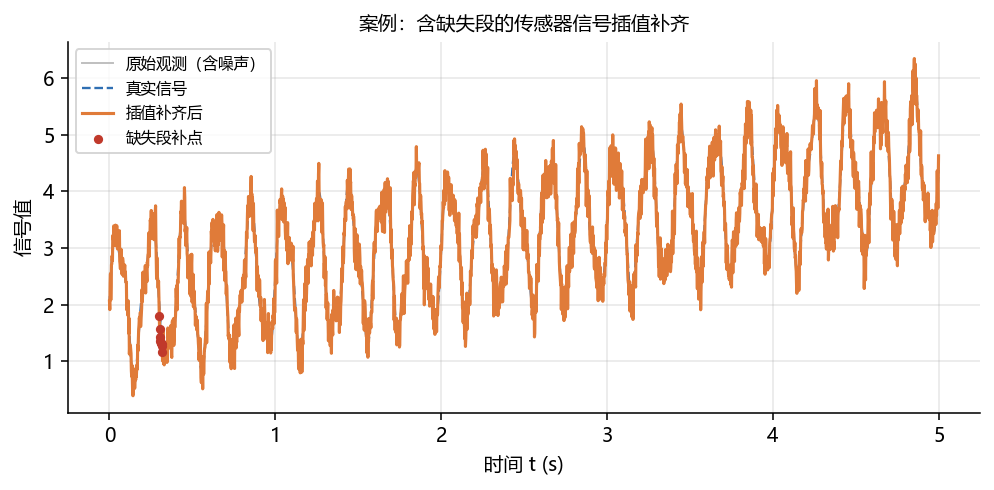
\includegraphics[keepaspectratio,alt={案例：含缺失段的信号插值补齐}]{figures/03-scipy/case_signal.png}}
\caption{案例：含缺失段的信号插值补齐}
\end{figure}

\subsection{用 FFT 找主频}\label{ux7528-fft-ux627eux4e3bux9891}

先做线性去趋势，消除漂移带来的低频泄漏，再取 \texttt{rfft}。

\begin{Shaded}
\begin{Highlighting}[]
\ImportTok{from}\NormalTok{ scipy.fft }\ImportTok{import}\NormalTok{ rfft, rfftfreq}
\NormalTok{coef }\OperatorTok{=}\NormalTok{ np.polyfit(t, y\_filled, }\DecValTok{1}\NormalTok{)}
\NormalTok{detrend }\OperatorTok{=}\NormalTok{ y\_filled }\OperatorTok{{-}}\NormalTok{ np.polyval(coef, t)}

\NormalTok{Y }\OperatorTok{=}\NormalTok{ rfft(detrend)}
\NormalTok{freqs }\OperatorTok{=}\NormalTok{ rfftfreq(N, }\DecValTok{1}\OperatorTok{/}\NormalTok{fs)}
\NormalTok{amps }\OperatorTok{=}\NormalTok{ np.}\BuiltInTok{abs}\NormalTok{(Y)}
\NormalTok{order }\OperatorTok{=}\NormalTok{ np.argsort(amps)[::}\OperatorTok{{-}}\DecValTok{1}\NormalTok{]}
\ControlFlowTok{for}\NormalTok{ k }\KeywordTok{in}\NormalTok{ order[:}\DecValTok{5}\NormalTok{]:}
    \BuiltInTok{print}\NormalTok{(}\SpecialStringTok{f"f=}\SpecialCharTok{\{}\NormalTok{freqs[k]}\SpecialCharTok{:.2f\}}\SpecialStringTok{ Hz  amp=}\SpecialCharTok{\{}\NormalTok{amps[k]}\SpecialCharTok{:.2f\}}\SpecialStringTok{"}\NormalTok{)}
\end{Highlighting}
\end{Shaded}

\begin{Shaded}
\begin{Highlighting}[]
\NormalTok{f=5.00 Hz  amp=1503.72}
\NormalTok{f=12.00 Hz  amp=371.19}
\NormalTok{f=0.20 Hz  amp=34.16}
\NormalTok{f=0.40 Hz  amp=30.74}
\NormalTok{f=19.60 Hz  amp=29.16}
\end{Highlighting}
\end{Shaded}

主峰在 5 Hz（次峰是 12
Hz）与建模时的真实频率完全一致；低频小峰来自去趋势后的残余。

\begin{figure}
\centering
\pandocbounded{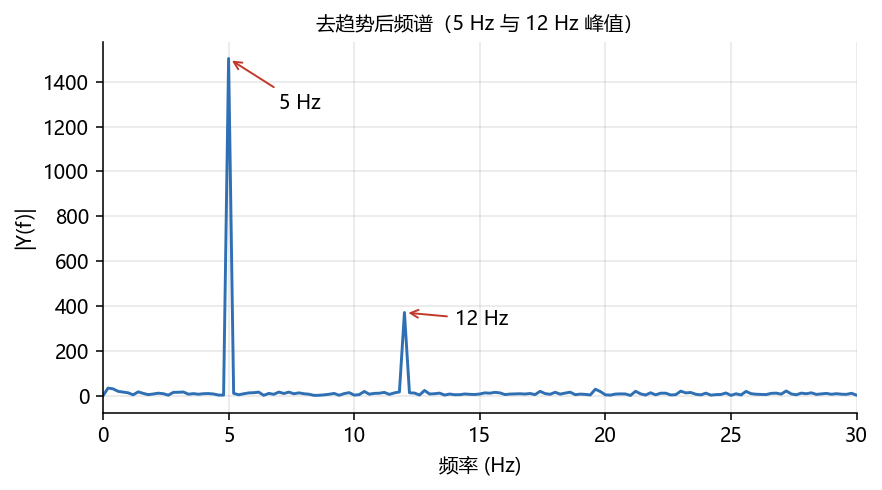
\includegraphics[keepaspectratio,alt={案例：去趋势后频谱}]{figures/03-scipy/case_fft.png}}
\caption{案例：去趋势后频谱}
\end{figure}

\subsection{\texorpdfstring{用 \texttt{curve\_fit}
拟合参数模型}{用 curve\_fit 拟合参数模型}}\label{ux7528-curve_fit-ux62dfux5408ux53c2ux6570ux6a21ux578b}

模型设为``常数 + 线性漂移 + 两个正弦''：

\[y(t)=c_1+c_2 t+A_1\sin(2\pi f_1 t+\varphi_1)+A_2\sin(2\pi f_2 t+\varphi_2)\]

\begin{Shaded}
\begin{Highlighting}[]
\ImportTok{from}\NormalTok{ scipy.optimize }\ImportTok{import}\NormalTok{ curve\_fit}

\KeywordTok{def}\NormalTok{ model(t, c1, c2, A1, f1, p1, A2, f2, p2):}
    \ControlFlowTok{return}\NormalTok{ c1 }\OperatorTok{+}\NormalTok{ c2}\OperatorTok{*}\NormalTok{t }\OperatorTok{+}\NormalTok{ A1}\OperatorTok{*}\NormalTok{np.sin(}\DecValTok{2}\OperatorTok{*}\NormalTok{np.pi}\OperatorTok{*}\NormalTok{f1}\OperatorTok{*}\NormalTok{t}\OperatorTok{+}\NormalTok{p1) }\OperatorTok{+}\NormalTok{ A2}\OperatorTok{*}\NormalTok{np.sin(}\DecValTok{2}\OperatorTok{*}\NormalTok{np.pi}\OperatorTok{*}\NormalTok{f2}\OperatorTok{*}\NormalTok{t}\OperatorTok{+}\NormalTok{p2)}

\NormalTok{popt, pcov }\OperatorTok{=}\NormalTok{ curve\_fit(model, t, y\_filled,}
\NormalTok{                       p0}\OperatorTok{=}\NormalTok{[}\DecValTok{2}\NormalTok{, }\FloatTok{0.5}\NormalTok{, }\FloatTok{1.2}\NormalTok{, }\DecValTok{5}\NormalTok{, }\DecValTok{0}\NormalTok{, }\FloatTok{0.3}\NormalTok{, }\DecValTok{12}\NormalTok{, }\DecValTok{0}\NormalTok{], maxfev}\OperatorTok{=}\DecValTok{50000}\NormalTok{)}
\NormalTok{perr }\OperatorTok{=}\NormalTok{ np.sqrt(np.diag(pcov))}
\BuiltInTok{print}\NormalTok{(}\StringTok{"拟合参数 ="}\NormalTok{, np.}\BuiltInTok{round}\NormalTok{(popt, }\DecValTok{4}\NormalTok{))}
\BuiltInTok{print}\NormalTok{(}\StringTok{"参数标准误 ="}\NormalTok{, np.}\BuiltInTok{round}\NormalTok{(perr, }\DecValTok{4}\NormalTok{))}
\NormalTok{resid }\OperatorTok{=}\NormalTok{ y\_filled }\OperatorTok{{-}}\NormalTok{ model(t, }\OperatorTok{*}\NormalTok{popt)}
\BuiltInTok{print}\NormalTok{(}\StringTok{"RMSE ="}\NormalTok{, }\BuiltInTok{round}\NormalTok{(}\BuiltInTok{float}\NormalTok{(np.sqrt(np.mean(resid}\OperatorTok{**}\DecValTok{2}\NormalTok{))), }\DecValTok{4}\NormalTok{))}
\BuiltInTok{print}\NormalTok{(}\StringTok{"f1 估计 ="}\NormalTok{, }\BuiltInTok{round}\NormalTok{(popt[}\DecValTok{3}\NormalTok{], }\DecValTok{3}\NormalTok{), }\StringTok{"   f2 估计 ="}\NormalTok{, }\BuiltInTok{round}\NormalTok{(popt[}\DecValTok{6}\NormalTok{], }\DecValTok{3}\NormalTok{))}
\end{Highlighting}
\end{Shaded}

\begin{Shaded}
\begin{Highlighting}[]
\NormalTok{拟合参数 = [ 1.9931  0.499   1.2042  5.0003 {-}0.0108  0.2977 12.0033 {-}0.064 ]}
\NormalTok{参数标准误 = [0.008  0.0028 0.0057 0.0005 0.0094 0.0057 0.0021 0.0382]}
\NormalTok{RMSE = 0.2009}
\NormalTok{f1 估计 = 5.0   f2 估计 = 12.003}
\end{Highlighting}
\end{Shaded}

拟合 \(f_1\approx5.00\) Hz、\(f_2\approx12.00\)
Hz，\(A_1\approx1.20\)、\(A_2\approx0.30\)，与真实模型高度一致；RMSE≈0.20
正是噪声标准差。

\begin{figure}
\centering
\pandocbounded{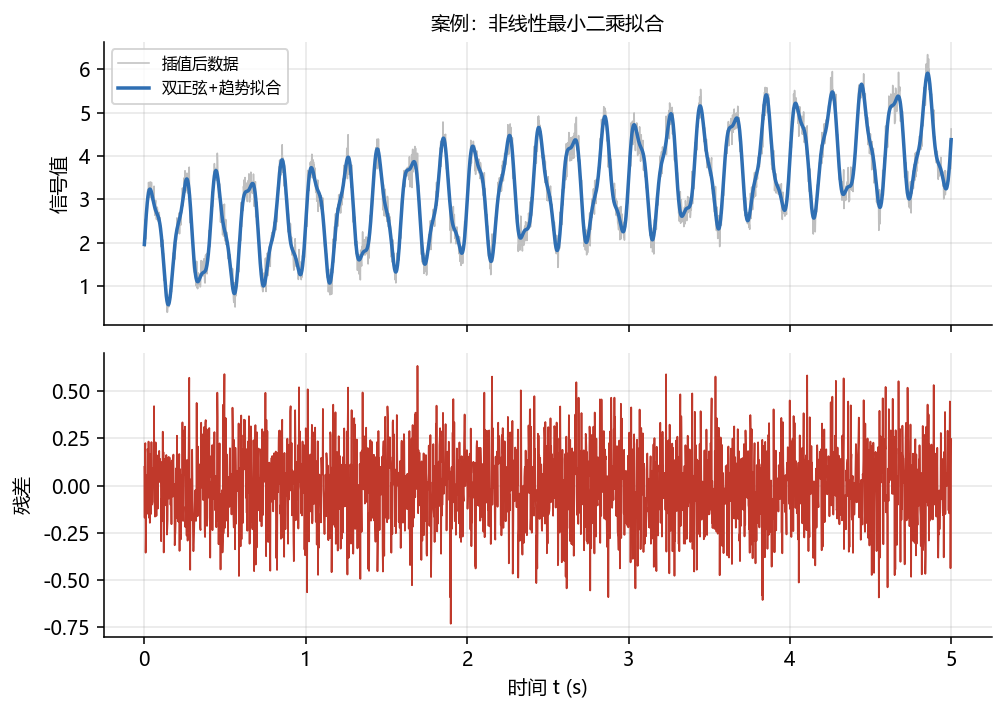
\includegraphics[keepaspectratio,alt={案例：拟合曲线与残差}]{figures/03-scipy/case_fit.png}}
\caption{案例：拟合曲线与残差}
\end{figure}

\subsection{\texorpdfstring{用 \texttt{trapezoid}
估计累积值}{用 trapezoid 估计累积值}}\label{ux7528-trapezoid-ux4f30ux8ba1ux7d2fux79efux503c}

\begin{Shaded}
\begin{Highlighting}[]
\ImportTok{from}\NormalTok{ scipy.integrate }\ImportTok{import}\NormalTok{ trapezoid}
\NormalTok{area }\OperatorTok{=}\NormalTok{ trapezoid(y\_filled, t)}
\BuiltInTok{print}\NormalTok{(}\StringTok{"5 秒内信号累积值 ="}\NormalTok{, }\BuiltInTok{round}\NormalTok{(}\BuiltInTok{float}\NormalTok{(area), }\DecValTok{4}\NormalTok{))}
\end{Highlighting}
\end{Shaded}

\begin{Shaded}
\begin{Highlighting}[]
\NormalTok{5 秒内信号累积值 = 16.1939}
\end{Highlighting}
\end{Shaded}

该值可理解为``总剂量/总能量''，是积分在工程中的一个典型用途。

\subsection{用 t
检验比较两段时间}\label{ux7528-t-ux68c0ux9a8cux6bd4ux8f83ux4e24ux6bb5ux65f6ux95f4}

线性漂移使后半段均值更高，用 \texttt{ttest\_ind} 验证。

\begin{Shaded}
\begin{Highlighting}[]
\ImportTok{from}\NormalTok{ scipy.stats }\ImportTok{import}\NormalTok{ ttest\_ind}
\NormalTok{g1 }\OperatorTok{=}\NormalTok{ y\_filled[(t }\OperatorTok{\textgreater{}=} \DecValTok{0}\NormalTok{) }\OperatorTok{\&}\NormalTok{ (t }\OperatorTok{\textless{}} \DecValTok{1}\NormalTok{)]}
\NormalTok{g2 }\OperatorTok{=}\NormalTok{ y\_filled[(t }\OperatorTok{\textgreater{}=} \DecValTok{4}\NormalTok{) }\OperatorTok{\&}\NormalTok{ (t }\OperatorTok{\textless{}} \DecValTok{5}\NormalTok{)]}
\NormalTok{res }\OperatorTok{=}\NormalTok{ ttest\_ind(g1, g2)}
\BuiltInTok{print}\NormalTok{(}\SpecialStringTok{f"前1s均值=}\SpecialCharTok{\{}\NormalTok{g1}\SpecialCharTok{.}\NormalTok{mean()}\SpecialCharTok{:.4f\}}\SpecialStringTok{, 后1s均值=}\SpecialCharTok{\{}\NormalTok{g2}\SpecialCharTok{.}\NormalTok{mean()}\SpecialCharTok{:.4f\}}\SpecialStringTok{"}\NormalTok{)}
\BuiltInTok{print}\NormalTok{(}\SpecialStringTok{f"t=}\SpecialCharTok{\{}\NormalTok{res}\SpecialCharTok{.}\NormalTok{statistic}\SpecialCharTok{:.3f\}}\SpecialStringTok{, p=}\SpecialCharTok{\{}\NormalTok{res}\SpecialCharTok{.}\NormalTok{pvalue}\SpecialCharTok{:.3e\}}\SpecialStringTok{"}\NormalTok{)}
\end{Highlighting}
\end{Shaded}

\begin{Shaded}
\begin{Highlighting}[]
\NormalTok{前1s均值=2.2442, 后1s均值=4.2493}
\NormalTok{t={-}35.601, p=7.475e{-}180}
\end{Highlighting}
\end{Shaded}

p
值极小，说明前、后两段均值差异在统计上高度显著------这正是题目设计的线性漂移所导致的。

\begin{figure}
\centering
\pandocbounded{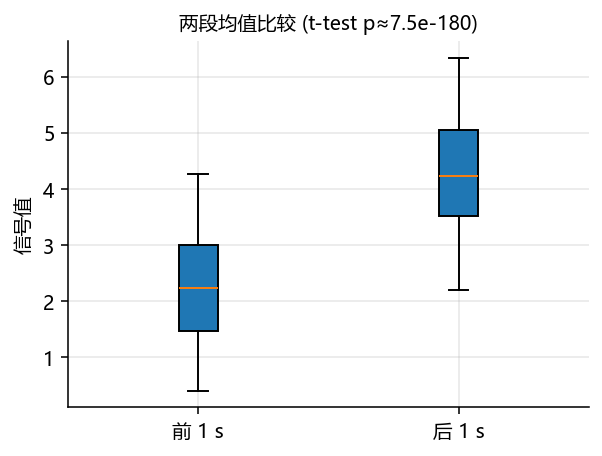
\includegraphics[keepaspectratio,alt={案例：两段时间均值比较}]{figures/03-scipy/case_stats.png}}
\caption{案例：两段时间均值比较}
\end{figure}

\subsection{小结}\label{ux5c0fux7ed3}

这个案例把本章五个工具包串成一条流水线：\textbf{插值补齐（03）→ FFT
定频（05）→ 非线性拟合（02）→ 积分（01）→ 假设检验（04）}。

{\def\LTcaptype{none} % do not increment counter
\begin{longtable}[]{@{}
  >{\raggedright\arraybackslash}p{(\linewidth - 4\tabcolsep) * \real{0.3333}}
  >{\raggedright\arraybackslash}p{(\linewidth - 4\tabcolsep) * \real{0.3333}}
  >{\raggedright\arraybackslash}p{(\linewidth - 4\tabcolsep) * \real{0.3333}}@{}}
\toprule\noalign{}
\begin{minipage}[b]{\linewidth}\raggedright
步骤
\end{minipage} & \begin{minipage}[b]{\linewidth}\raggedright
工具
\end{minipage} & \begin{minipage}[b]{\linewidth}\raggedright
产出
\end{minipage} \\
\midrule\noalign{}
\endhead
\bottomrule\noalign{}
\endlastfoot
补齐缺失 & \texttt{CubicSpline} & 完整时间序列 \\
频谱分析 & \texttt{rfft}/\texttt{rfftfreq} & 主频 5 Hz、12 Hz \\
参数化建模 & \texttt{curve\_fit} &
\(c_1,c_2,A_1,f_1,\varphi_1,A_2,f_2,\varphi_2\) \\
累积量 & \texttt{trapezoid} & 16.1939 \\
均值比较 & \texttt{ttest\_ind} & t=-35.60，p≈7.5e-180 \\
\end{longtable}
}

\subsection{拓展任务}\label{ux62d3ux5c55ux4efbux52a1-5}

\begin{enumerate}
\def\labelenumi{\arabic{enumi}.}
\tightlist
\item
  把缺失段加宽（如 0.30--0.50 s），观察插值误差如何变化；
\item
  用 \texttt{scipy.signal.butter} 低通（截止 10 Hz）滤除 12 Hz
  分量后重新拟合，比较残差；
\item
  把``前 1 s vs 后 1 s''换成``前 2.5 s vs 后 2.5 s''，看 p
  值变化并解释；
\item
  用 statsmodels 对三段时间做单因素 ANOVA + Tukey 事后比较。
\end{enumerate}

\subsection{延伸阅读}\label{ux5ef6ux4f38ux9605ux8bfb-15}

\begin{itemize}
\tightlist
\item
  SciPy 插值 / FFT / 优化官方文档见各节``官方文档/参考入口''。
\item
  信号处理完整示例：https://docs.scipy.org/doc/scipy/tutorial/fft.html
\item
  statsmodels 多重比较：https://www.statsmodels.org/stable/stats.html
\end{itemize}

\section{07
常见误区与技巧}\label{ux5e38ux89c1ux8befux533aux4e0eux6280ux5de7-2}

\begin{quote}
本章为新增``查漏补缺''页：把学生在 SciPy
上最容易踩的坑集中列出，并给出正确写法、性能与调试建议。
\end{quote}

\subsection{1.
高频误区速查表}\label{ux9ad8ux9891ux8befux533aux901fux67e5ux8868-2}

{\def\LTcaptype{none} % do not increment counter
\begin{longtable}[]{@{}
  >{\raggedright\arraybackslash}p{(\linewidth - 6\tabcolsep) * \real{0.2500}}
  >{\raggedright\arraybackslash}p{(\linewidth - 6\tabcolsep) * \real{0.2500}}
  >{\raggedright\arraybackslash}p{(\linewidth - 6\tabcolsep) * \real{0.2500}}
  >{\raggedright\arraybackslash}p{(\linewidth - 6\tabcolsep) * \real{0.2500}}@{}}
\toprule\noalign{}
\begin{minipage}[b]{\linewidth}\raggedright
\#
\end{minipage} & \begin{minipage}[b]{\linewidth}\raggedright
误区 / 错误写法
\end{minipage} & \begin{minipage}[b]{\linewidth}\raggedright
正确做法
\end{minipage} & \begin{minipage}[b]{\linewidth}\raggedright
原因
\end{minipage} \\
\midrule\noalign{}
\endhead
\bottomrule\noalign{}
\endlastfoot
1 & \texttt{from\ scipy.integrate\ import\ trapz} & 用
\texttt{trapezoid} & SciPy 1.15 已移除 \texttt{trapz} \\
2 & \texttt{odeint} 写 \texttt{func(t,\ y)} & 写成 \texttt{func(y,\ t)}
& \texttt{odeint} 的签名是 \texttt{(y,\ t)}，\texttt{solve\_ivp} 才是
\texttt{(t,\ y)} \\
3 & \texttt{solve\_ivp(f,\ 0,\ 5,\ y0)} &
\texttt{solve\_ivp(f,\ (0,5),\ y0)} & \texttt{t\_span} 是二元组 \\
4 & \texttt{quad(f,0,1)} 然后当数组用 &
\texttt{value,\ err\ =\ quad(...)} & \texttt{quad} 返回
\texttt{(value,\ error)} 元组 \\
5 & 用 \texttt{brent} 求根 & 求根用
\texttt{brentq}/\texttt{fsolve}/\texttt{root} & \texttt{brent}
求极小值，\texttt{brentq} 求根 \\
6 & \texttt{linprog(c)} 直接当最大化用 & 最大化时 \texttt{c} 取负 &
\texttt{linprog} 默认最小化 \\
7 & \texttt{linear\_sum\_assignment} 后直接 \texttt{cost.sum()} &
\texttt{cost{[}row\_ind,\ col\_ind{]}.sum()} &
返回索引配对，需用索引取成本 \\
8 & \texttt{minimize} 约束写成 \texttt{fun(x)\ \textless{}=\ 0} &
\texttt{ineq} 表示 \texttt{fun(x)\ \textgreater{}=\ 0} &
约束符号方向易反 \\
9 & 不给 \texttt{p0} 就 \texttt{curve\_fit} & 给接近真实值的初值 &
非线性最小二乘对初值敏感 \\
10 & 用 \texttt{interp2d} 做新代码 & 用
\texttt{RegularGridInterpolator}/\texttt{griddata} & \texttt{interp2d}
已废弃 \\
11 & 对噪声数据做样条插值 & 改为 \texttt{curve\_fit}/\texttt{np.polyfit}
& 插值会``穿过噪声'' \\
12 & \texttt{griddata} 在凸包外直接外推 & 自行判断并处理 \texttt{nan} &
\texttt{griddata} 不默认外推 \\
13 & \texttt{butter(Wn=cutoff)} & \texttt{Wn\ =\ cutoff\ /\ (fs/2)} &
\texttt{Wn} 是归一化频率 \\
14 & 把 \texttt{fft} 幅值当真实幅度 & 单边需乘 \(2/N\)；或用
\texttt{rfft} 后归一化 & \texttt{fft} 未除以 \(N\) \\
15 & 统计 p\textless0.05 就说``差异很大'' & 同时看效应量/置信区间 & p
值不度量重要性 \\
16 & 不做正态性检验就小样本 t 检验 & 小样本先 \texttt{shapiro} & t
检验假设近似正态 \\
17 & ANOVA 显著后不做事后比较 & 用 \texttt{pairwise\_tukeyhsd} &
需找具体差异组 \\
18 & 随机模拟不设种子 & \texttt{rng\ =\ np.random.default\_rng(seed)} &
便于复现与讨论 \\
\end{longtable}
}

\subsection{2.
原理级难点：版本迁移与新接口}\label{ux539fux7406ux7ea7ux96beux70b9ux7248ux672cux8fc1ux79fbux4e0eux65b0ux63a5ux53e3}

\begin{quote}
SciPy
迭代较快，老教材中的某些函数已改名或废弃。写新代码时以官方最新文档为准。
\end{quote}

{\def\LTcaptype{none} % do not increment counter
\begin{longtable}[]{@{}
  >{\raggedright\arraybackslash}p{(\linewidth - 4\tabcolsep) * \real{0.3333}}
  >{\raggedright\arraybackslash}p{(\linewidth - 4\tabcolsep) * \real{0.3333}}
  >{\raggedright\arraybackslash}p{(\linewidth - 4\tabcolsep) * \real{0.3333}}@{}}
\toprule\noalign{}
\begin{minipage}[b]{\linewidth}\raggedright
老写法
\end{minipage} & \begin{minipage}[b]{\linewidth}\raggedright
新写法
\end{minipage} & \begin{minipage}[b]{\linewidth}\raggedright
说明
\end{minipage} \\
\midrule\noalign{}
\endhead
\bottomrule\noalign{}
\endlastfoot
\texttt{scipy.integrate.trapz} & \texttt{scipy.integrate.trapezoid} &
同名函数改名 \\
\texttt{scipy.integrate.odeint}（仍可用） & 推荐 \texttt{solve\_ivp} &
新接口更灵活，支持事件/设置 \\
\texttt{scipy.optimize.leastsq}（仍可用） & 推荐 \texttt{curve\_fit} &
接口更友好，返回协方差 \\
\texttt{scipy.optimize.fmin}（仍可用） &
\texttt{minimize(method=\textquotesingle{}Nelder-Mead\textquotesingle{})}
& 统一入口 \\
\texttt{scipy.interpolate.interp2d} & \texttt{RegularGridInterpolator} &
\texttt{interp2d} 已废弃 \\
\texttt{scipy.fftpack} & \texttt{scipy.fft} & 新模块，接口更好 \\
\end{longtable}
}

\subsection{3. 性能技巧}\label{ux6027ux80fdux6280ux5de7-2}

\begin{itemize}
\tightlist
\item
  \textbf{向量化优先}：能用 NumPy 数组一次算完就不要 Python 循环；
\item
  \textbf{FFT 用
  \texttt{rfft}}：实数信号只用一半复数，速度与内存都省一半；
\item
  \textbf{插值选方法}：线性插值最快，三次样条更光滑但更慢；大数据散点可先
  \texttt{cKDTree} 再 \texttt{griddata}；
\item
  \textbf{\texttt{curve\_fit} 给 \texttt{maxfev}}：复杂模型设
  \texttt{maxfev=50000} 避免``达到最大调用次数''而失败；
\item
  \textbf{积分用 \texttt{quad}
  而非固定步长}：自适应能在光滑区间少算、在陡峭区间加密；
\item
  \textbf{优化设
  \texttt{bounds}/\texttt{constraints}}：有约束问题别用无约束方法，容易跑出物理合理区间；
\item
  \textbf{多进程并行}：\texttt{scipy.optimize.differential\_evolution}
  等全局方法天然可并行，用 \texttt{workers} 参数。
\end{itemize}

\subsection{4. 调试建议}\label{ux8c03ux8bd5ux5efaux8bae-2}

\begin{enumerate}
\def\labelenumi{\arabic{enumi}.}
\tightlist
\item
  \textbf{打印形状/版本}：\texttt{print(x.shape,\ scipy.\_\_version\_\_)}，先确认输入维度正确；
\item
  \textbf{检查收敛标志}：\texttt{root}、\texttt{minimize}、\texttt{curve\_fit}
  都看 \texttt{success}/\texttt{message}，别只看结果；
\item
  \textbf{给初值/区间}：\texttt{curve\_fit} 用
  \texttt{p0}；\texttt{brentq} 用 \texttt{brack}；\texttt{minimize}
  用多组初值；
\item
  \textbf{固定随机种子}：\texttt{default\_rng(seed)}，保证课堂演示与作业可复现；
\item
  \textbf{异常值/NaN}：先用 \texttt{np.isnan}/\texttt{np.isinf}
  检查数据，再做插值/拟合；
\item
  \textbf{用图直观检查}：把数据、插值曲线、拟合曲线、频谱画出来，问题一眼可见；
\item
  \textbf{测试小数据}：先用 5
  个点验证函数是否返回合理，再放大到真实数据。
\end{enumerate}

\subsection{5. 自测清单}\label{ux81eaux6d4bux6e05ux5355}

\begin{itemize}
\tightlist
\item[$\square$]
  能用 \texttt{quad}/\texttt{dblquad}/\texttt{trapezoid} 求定积分；
\item[$\square$]
  能把二阶 ODE 化成一阶方程组并用 \texttt{odeint}/\texttt{solve\_ivp}
  求解；
\item[$\square$]
  能用 \texttt{brentq} 求根、\texttt{brent} 求极小值，并说清区别；
\item[$\square$]
  能用
  \texttt{minimize}/\texttt{linprog}/\texttt{linear\_sum\_assignment}
  解决无约束/线性规划/指派问题；
\item[$\square$]
  能用 \texttt{curve\_fit} 拟合参数并读取 \texttt{pcov}；
\item[$\square$]
  能用
  \texttt{CubicSpline}/\texttt{RegularGridInterpolator}/\texttt{griddata}
  完成一维/二维/散点插值；
\item[$\square$]
  能说出插值 vs 拟合的区别；
\item[$\square$]
  能用
  \texttt{shapiro}/\texttt{ttest\_ind}/\texttt{ttest\_rel}/\texttt{chi2\_contingency}/\texttt{f\_oneway}
  完成检验并解读 p 值；
\item[$\square$]
  能用 \texttt{rfft}/\texttt{rfftfreq} 找主频，用
  \texttt{butter}+\texttt{lfilter} 做滤波；
\item[$\square$]
  能独立完成 06 综合案例并解释每一步。
\end{itemize}

\subsection{延伸阅读}\label{ux5ef6ux4f38ux9605ux8bfb-16}

\begin{itemize}
\tightlist
\item
  SciPy 官方``Release
  notes''查看版本变更：https://docs.scipy.org/doc/scipy/release.html
\item
  SciPy 性能 / 高阶技巧：https://scipy-lectures.org/
\item
  SciPy
  Cookbook（老但仍有参考价值）：https://scipy.github.io/old-wiki/pages/Cookbook/
\end{itemize}

\newpage

%% 由 build/emit_tex.py 生成（生成物，勿手改）；定制请放 user_style.tex / user_meta.yaml
\chapter{Pandas及其基本使用}\label{pandasux53caux5176ux57faux672cux4f7fux7528}

\section{01 基础数据结构：Series 与
DataFrame}\label{ux57faux7840ux6570ux636eux7ed3ux6784series-ux4e0e-dataframe}

\begin{quote}
本节对应原版 4.1 的内容，并增补学习目标、常见误区、思考题与延伸阅读。
\end{quote}

\subsection{本节目标}\label{ux672cux8282ux76eeux6807-18}

\begin{itemize}
\tightlist
\item
  理解 \texttt{Series}（一维带标签）与
  \texttt{DataFrame}（二维表格）两种核心结构；
\item
  会用列表、NumPy 数组、字典创建 Series 与 DataFrame，并指定
  \texttt{index}/\texttt{columns}；
\item
  掌握 \texttt{.loc}（按标签）与 \texttt{.iloc}（按位置）的区别；
\item
  会用布尔索引 + \texttt{\&} / \texttt{\textbar{}} /
  \texttt{\textasciitilde{}} 做多条件筛选；
\item
  会用 \texttt{sort\_values}、\texttt{concat}、\texttt{merge}
  做排序与合并；
\item
  会用 \texttt{date\_range} 生成日期索引，并按日期筛选。
\end{itemize}

\subsection{先修}\label{ux5148ux4fee-11}

\begin{itemize}
\tightlist
\item
  Python 列表、字典、推导式；第 1 章 NumPy
  数组概念（\texttt{ndarray}、\texttt{shape}、\texttt{dtype}）。
\end{itemize}

\begin{center}\rule{0.5\linewidth}{0.5pt}\end{center}

\subsection{官方文档 /
参考入口}\label{ux5b98ux65b9ux6587ux6863-ux53c2ux8003ux5165ux53e3-5}

\begin{itemize}
\tightlist
\item
  Pandas 官方入门：https://pandas.pydata.org/docs/user\_guide/10min.html
\item
  Pandas Series
  参考：https://pandas.pydata.org/docs/reference/api/pandas.Series.html
\item
  Pandas DataFrame
  参考：https://pandas.pydata.org/docs/reference/api/pandas.DataFrame.html
\end{itemize}

\begin{center}\rule{0.5\linewidth}{0.5pt}\end{center}

\subsection{1.1 为什么用 Pandas}\label{ux4e3aux4ec0ux4e48ux7528-pandas}

NumPy 的 \texttt{ndarray}
擅长向量化数值计算，但没有``列名/行名/标签''的概念，也缺少缺失值、分组、透视等表格能力。Pandas
在 NumPy 之上提供：

{\def\LTcaptype{none} % do not increment counter
\begin{longtable}[]{@{}lll@{}}
\toprule\noalign{}
特性 & NumPy ndarray & Pandas Series/DataFrame \\
\midrule\noalign{}
\endhead
\bottomrule\noalign{}
\endlastfoot
维度 & 任意 N 维 & 1 维（Series）/ 2 维（DataFrame） \\
标签 & 只有整数位置索引 & 可自定义 \texttt{index}（行）与
\texttt{columns}（列） \\
缺失值 & 常需 \texttt{np.nan} + 手写 &
\texttt{isna}/\texttt{fillna}/\texttt{dropna} 成套 \\
分组/透视 & 需手写 & \texttt{groupby}/\texttt{pivot\_table} \\
与 Excel/SQL 接近程度 & 低 & 高 \\
\end{longtable}
}

\begin{center}\rule{0.5\linewidth}{0.5pt}\end{center}

\subsection{1.2 Series}\label{series}

\subsubsection{1.2.1 创建 Series}\label{ux521bux5efa-series}

\begin{Shaded}
\begin{Highlighting}[]
\ImportTok{import}\NormalTok{ pandas }\ImportTok{as}\NormalTok{ pd}
\ImportTok{import}\NormalTok{ numpy }\ImportTok{as}\NormalTok{ np}

\NormalTok{s1 }\OperatorTok{=}\NormalTok{ pd.Series([}\DecValTok{1}\NormalTok{, }\DecValTok{2}\NormalTok{, }\DecValTok{3}\NormalTok{, }\DecValTok{4}\NormalTok{, }\DecValTok{5}\NormalTok{])          }\CommentTok{\# 列表}
\NormalTok{s2 }\OperatorTok{=}\NormalTok{ pd.Series(np.array([}\DecValTok{1}\NormalTok{, }\DecValTok{2}\NormalTok{, }\DecValTok{3}\NormalTok{, }\DecValTok{4}\NormalTok{, }\DecValTok{5}\NormalTok{]))  }\CommentTok{\# NumPy 数组}
\NormalTok{s3 }\OperatorTok{=}\NormalTok{ pd.Series([}\DecValTok{1}\NormalTok{, }\DecValTok{2}\NormalTok{, }\DecValTok{3}\NormalTok{, }\DecValTok{4}\NormalTok{, }\DecValTok{5}\NormalTok{], index}\OperatorTok{=}\NormalTok{[}\StringTok{\textquotesingle{}a\textquotesingle{}}\NormalTok{, }\StringTok{\textquotesingle{}b\textquotesingle{}}\NormalTok{, }\StringTok{\textquotesingle{}c\textquotesingle{}}\NormalTok{, }\StringTok{\textquotesingle{}d\textquotesingle{}}\NormalTok{, }\StringTok{\textquotesingle{}e\textquotesingle{}}\NormalTok{])}
\NormalTok{s4 }\OperatorTok{=}\NormalTok{ pd.Series(\{}\StringTok{\textquotesingle{}a\textquotesingle{}}\NormalTok{: }\DecValTok{1}\NormalTok{, }\StringTok{\textquotesingle{}b\textquotesingle{}}\NormalTok{: }\DecValTok{2}\NormalTok{, }\StringTok{\textquotesingle{}c\textquotesingle{}}\NormalTok{: }\DecValTok{3}\NormalTok{, }\StringTok{\textquotesingle{}d\textquotesingle{}}\NormalTok{: }\DecValTok{4}\NormalTok{, }\StringTok{\textquotesingle{}e\textquotesingle{}}\NormalTok{: }\DecValTok{5}\NormalTok{\})  }\CommentTok{\# 字典}
\end{Highlighting}
\end{Shaded}

\begin{Shaded}
\begin{Highlighting}[]
\NormalTok{\#\# s3}
\NormalTok{    a    1}
\NormalTok{    b    2}
\NormalTok{    c    3}
\NormalTok{    d    4}
\NormalTok{    e    5}
\NormalTok{    dtype: int64}
\end{Highlighting}
\end{Shaded}

\begin{quote}
不指定索引时，pandas 自动生成从 0 开始的整数索引。
\end{quote}

\subsubsection{1.2.2 访问与修改}\label{ux8bbfux95eeux4e0eux4feeux6539}

\begin{Shaded}
\begin{Highlighting}[]
\BuiltInTok{print}\NormalTok{(s3[}\StringTok{\textquotesingle{}a\textquotesingle{}}\NormalTok{])       }\CommentTok{\# 按标签}
\BuiltInTok{print}\NormalTok{(s3.iloc[}\DecValTok{0}\NormalTok{])    }\CommentTok{\# 按位置（推荐，避免整数歧义）}

\NormalTok{s3[}\StringTok{\textquotesingle{}a\textquotesingle{}}\NormalTok{] }\OperatorTok{=} \DecValTok{10}         \CommentTok{\# 按标签修改}
\NormalTok{s3.iloc[}\DecValTok{0}\NormalTok{] }\OperatorTok{=} \DecValTok{100}     \CommentTok{\# 按位置修改}
\BuiltInTok{print}\NormalTok{(s3)}
\end{Highlighting}
\end{Shaded}

\begin{Shaded}
\begin{Highlighting}[]
\NormalTok{1}
\NormalTok{1}
\NormalTok{    a    100}
\NormalTok{    b      2}
\NormalTok{    c      3}
\NormalTok{    d      4}
\NormalTok{    e      5}
\NormalTok{    dtype: int64}
\end{Highlighting}
\end{Shaded}

\begin{quote}
新版 pandas 中，用 \texttt{s{[}0{]}}
取``位置''会触发弃用警告；位置访问请统一
\texttt{s.iloc{[}0{]}}，标签访问用
\texttt{s{[}\textquotesingle{}a\textquotesingle{}{]}}。
\end{quote}

\subsubsection{1.2.3 索引切片}\label{ux7d22ux5f15ux5207ux7247}

\begin{Shaded}
\begin{Highlighting}[]
\BuiltInTok{print}\NormalTok{(s3[}\StringTok{\textquotesingle{}a\textquotesingle{}}\NormalTok{:}\StringTok{\textquotesingle{}c\textquotesingle{}}\NormalTok{])   }\CommentTok{\# 基于标签的切片：闭区间}
\NormalTok{s5 }\OperatorTok{=}\NormalTok{ pd.Series([}\DecValTok{1}\NormalTok{, }\DecValTok{2}\NormalTok{, }\DecValTok{3}\NormalTok{, }\DecValTok{4}\NormalTok{, }\DecValTok{5}\NormalTok{], index}\OperatorTok{=}\NormalTok{[}\DecValTok{0}\NormalTok{, }\DecValTok{1}\NormalTok{, }\DecValTok{2}\NormalTok{, }\DecValTok{3}\NormalTok{, }\DecValTok{4}\NormalTok{])}
\BuiltInTok{print}\NormalTok{(s5[}\DecValTok{0}\NormalTok{:}\DecValTok{3}\NormalTok{])       }\CommentTok{\# 整数索引时按位置切片}
\end{Highlighting}
\end{Shaded}

\begin{Shaded}
\begin{Highlighting}[]
\NormalTok{    a    100}
\NormalTok{    b      2}
\NormalTok{    c      3}
\NormalTok{    dtype: int64}
\NormalTok{0    1}
\NormalTok{1    2}
\NormalTok{2    3}
\NormalTok{dtype: int64}
\end{Highlighting}
\end{Shaded}

\begin{quote}
注意：标签切片\textbf{包含终点}（比如
\texttt{\textquotesingle{}a\textquotesingle{}:\textquotesingle{}c\textquotesingle{}}
含 c），而 Python 列表切片不含终点。
\end{quote}

\subsubsection{1.2.4
运算与索引对齐}\label{ux8fd0ux7b97ux4e0eux7d22ux5f15ux5bf9ux9f50}

\begin{Shaded}
\begin{Highlighting}[]
\NormalTok{s6 }\OperatorTok{=}\NormalTok{ s3 }\OperatorTok{+} \DecValTok{10}
\BuiltInTok{print}\NormalTok{(s6)}

\NormalTok{s7 }\OperatorTok{=}\NormalTok{ pd.Series([}\DecValTok{1}\NormalTok{, }\DecValTok{2}\NormalTok{, }\DecValTok{3}\NormalTok{], index}\OperatorTok{=}\NormalTok{[}\StringTok{\textquotesingle{}a\textquotesingle{}}\NormalTok{, }\StringTok{\textquotesingle{}c\textquotesingle{}}\NormalTok{, }\StringTok{\textquotesingle{}e\textquotesingle{}}\NormalTok{])}
\BuiltInTok{print}\NormalTok{(s3 }\OperatorTok{+}\NormalTok{ s7)        }\CommentTok{\# 按共同索引对齐；缺失处为 NaN}
\end{Highlighting}
\end{Shaded}

\begin{Shaded}
\begin{Highlighting}[]
\NormalTok{\#\# s3 + 10}
\NormalTok{    a    110}
\NormalTok{    b     12}
\NormalTok{    c     13}
\NormalTok{    d     14}
\NormalTok{    e     15}
\NormalTok{    dtype: int64}

\NormalTok{\#\# s3 + s7}
\NormalTok{    a    101.0}
\NormalTok{    b      NaN}
\NormalTok{    c      5.0}
\NormalTok{    d      NaN}
\NormalTok{    e      8.0}
\NormalTok{    dtype: float64}
\end{Highlighting}
\end{Shaded}

\begin{quote}
两个 Series 相加时，索引会\textbf{对齐}；没有共同索引的位置得到
\texttt{NaN}，这是 Pandas 的重要语义。
\end{quote}

\subsubsection{1.2.5
常用属性与方法}\label{ux5e38ux7528ux5c5eux6027ux4e0eux65b9ux6cd5}

\begin{Shaded}
\begin{Highlighting}[]
\BuiltInTok{print}\NormalTok{(s3.index)                }\CommentTok{\# Index([\textquotesingle{}a\textquotesingle{}, \textquotesingle{}b\textquotesingle{}, \textquotesingle{}c\textquotesingle{}, \textquotesingle{}d\textquotesingle{}, \textquotesingle{}e\textquotesingle{}], dtype=\textquotesingle{}object\textquotesingle{})}
\BuiltInTok{print}\NormalTok{(s3.values)               }\CommentTok{\# array([100,   2,   3,   4,   5])}
\BuiltInTok{print}\NormalTok{(s3.describe())           }\CommentTok{\# 统计摘要}
\BuiltInTok{print}\NormalTok{(s3.head(}\DecValTok{2}\NormalTok{), s3.tail(}\DecValTok{2}\NormalTok{))  }\CommentTok{\# 头/尾}
\BuiltInTok{print}\NormalTok{(s3.isnull(), s3.notnull())}
\end{Highlighting}
\end{Shaded}

\begin{Shaded}
\begin{Highlighting}[]
\NormalTok{Index([\textquotesingle{}a\textquotesingle{}, \textquotesingle{}b\textquotesingle{}, \textquotesingle{}c\textquotesingle{}, \textquotesingle{}d\textquotesingle{}, \textquotesingle{}e\textquotesingle{}], dtype=\textquotesingle{}object\textquotesingle{})}
\NormalTok{[100   2   3   4   5]}
\NormalTok{count     5.000000}
\NormalTok{mean     22.800000}
\NormalTok{std      43.170592}
\NormalTok{min       2.000000}
\NormalTok{25\%       3.000000}
\NormalTok{50\%       4.000000}
\NormalTok{75\%       5.000000}
\NormalTok{max     100.000000}
\NormalTok{dtype: float64}
\NormalTok{    a    100}
\NormalTok{    b      2}
\NormalTok{    dtype: int64}
\NormalTok{    d    4}
\NormalTok{    e    5}
\NormalTok{    dtype: int64}
\NormalTok{    a    False}
\NormalTok{    b    False}
\NormalTok{    c    False}
\NormalTok{    d    False}
\NormalTok{    e    False}
\NormalTok{    dtype: bool}
\end{Highlighting}
\end{Shaded}

\begin{quote}
小提醒：统计方法（\texttt{describe}/\texttt{mean}/\texttt{std}
等）会\textbf{自动忽略 NaN}；\texttt{value\_counts()}（注意是复数
counts）统计每个取值出现次数。
\end{quote}

\begin{center}\rule{0.5\linewidth}{0.5pt}\end{center}

\subsection{1.3 DataFrame}\label{dataframe}

\subsubsection{1.3.1 创建 DataFrame}\label{ux521bux5efa-dataframe}

\begin{Shaded}
\begin{Highlighting}[]
\CommentTok{\#\# 1) 二维列表}
\NormalTok{df1 }\OperatorTok{=}\NormalTok{ pd.DataFrame([[}\DecValTok{1}\NormalTok{, }\DecValTok{2}\NormalTok{, }\DecValTok{3}\NormalTok{], [}\DecValTok{4}\NormalTok{, }\DecValTok{5}\NormalTok{, }\DecValTok{6}\NormalTok{], [}\DecValTok{7}\NormalTok{, }\DecValTok{8}\NormalTok{, }\DecValTok{9}\NormalTok{]], columns}\OperatorTok{=}\NormalTok{[}\StringTok{\textquotesingle{}A\textquotesingle{}}\NormalTok{, }\StringTok{\textquotesingle{}B\textquotesingle{}}\NormalTok{, }\StringTok{\textquotesingle{}C\textquotesingle{}}\NormalTok{])}

\CommentTok{\#\# 2) 字典（键为列名）}
\NormalTok{df2 }\OperatorTok{=}\NormalTok{ pd.DataFrame(\{}\StringTok{\textquotesingle{}A\textquotesingle{}}\NormalTok{: [}\DecValTok{1}\NormalTok{, }\DecValTok{2}\NormalTok{, }\DecValTok{3}\NormalTok{], }\StringTok{\textquotesingle{}B\textquotesingle{}}\NormalTok{: [}\DecValTok{4}\NormalTok{, }\DecValTok{5}\NormalTok{, }\DecValTok{6}\NormalTok{], }\StringTok{\textquotesingle{}C\textquotesingle{}}\NormalTok{: [}\DecValTok{7}\NormalTok{, }\DecValTok{8}\NormalTok{, }\DecValTok{9}\NormalTok{]\})}

\CommentTok{\#\# 3) 字典列表（每个字典一行）}
\NormalTok{df3 }\OperatorTok{=}\NormalTok{ pd.DataFrame([\{}\StringTok{\textquotesingle{}A\textquotesingle{}}\NormalTok{: }\DecValTok{1}\NormalTok{, }\StringTok{\textquotesingle{}B\textquotesingle{}}\NormalTok{: }\DecValTok{4}\NormalTok{, }\StringTok{\textquotesingle{}C\textquotesingle{}}\NormalTok{: }\DecValTok{7}\NormalTok{\},}
\NormalTok{                    \{}\StringTok{\textquotesingle{}A\textquotesingle{}}\NormalTok{: }\DecValTok{2}\NormalTok{, }\StringTok{\textquotesingle{}B\textquotesingle{}}\NormalTok{: }\DecValTok{5}\NormalTok{, }\StringTok{\textquotesingle{}C\textquotesingle{}}\NormalTok{: }\DecValTok{8}\NormalTok{\},}
\NormalTok{                    \{}\StringTok{\textquotesingle{}A\textquotesingle{}}\NormalTok{: }\DecValTok{3}\NormalTok{, }\StringTok{\textquotesingle{}B\textquotesingle{}}\NormalTok{: }\DecValTok{6}\NormalTok{, }\StringTok{\textquotesingle{}C\textquotesingle{}}\NormalTok{: }\DecValTok{9}\NormalTok{\}])}

\CommentTok{\#\# 4) NumPy 二维数组}
\NormalTok{df4 }\OperatorTok{=}\NormalTok{ pd.DataFrame(np.array([[}\DecValTok{1}\NormalTok{, }\DecValTok{2}\NormalTok{, }\DecValTok{3}\NormalTok{], [}\DecValTok{4}\NormalTok{, }\DecValTok{5}\NormalTok{, }\DecValTok{6}\NormalTok{], [}\DecValTok{7}\NormalTok{, }\DecValTok{8}\NormalTok{, }\DecValTok{9}\NormalTok{]]), columns}\OperatorTok{=}\NormalTok{[}\StringTok{\textquotesingle{}A\textquotesingle{}}\NormalTok{, }\StringTok{\textquotesingle{}B\textquotesingle{}}\NormalTok{, }\StringTok{\textquotesingle{}C\textquotesingle{}}\NormalTok{])}
\BuiltInTok{print}\NormalTok{(df1)}
\BuiltInTok{print}\NormalTok{(df2)}
\end{Highlighting}
\end{Shaded}

\begin{Shaded}
\begin{Highlighting}[]
\NormalTok{   A  B  C}
\NormalTok{0  1  2  3}
\NormalTok{1  4  5  6}
\NormalTok{2  7  8  9}
\NormalTok{   A  B  C}
\NormalTok{0  1  4  7}
\NormalTok{1  2  5  8}
\NormalTok{2  3  6  9}
\end{Highlighting}
\end{Shaded}

\begin{quote}
字典创建时键作为\textbf{列名}，各列等长；字典列表创建时每个字典是\textbf{一行}。
\end{quote}

\subsubsection{1.3.2 从文件读取}\label{ux4eceux6587ux4ef6ux8bfbux53d6}

\begin{Shaded}
\begin{Highlighting}[]
\CommentTok{\#\# pandas 提供了多种读取接口}
\CommentTok{\#\# df\_csv = pd.read\_csv(\textquotesingle{}data.csv\textquotesingle{})}
\CommentTok{\#\# df\_excel = pd.read\_excel(\textquotesingle{}data.xlsx\textquotesingle{})}
\CommentTok{\#\# df\_json = pd.read\_json(\textquotesingle{}data.json\textquotesingle{})}
\end{Highlighting}
\end{Shaded}

\begin{quote}
读取 Excel 需要 \texttt{openpyxl}（.xlsx）或 \texttt{xlrd}（.xls）；CSV
是课程中最常用的交换格式。
\end{quote}

\subsubsection{1.3.3 访问数据}\label{ux8bbfux95eeux6570ux636e}

\begin{Shaded}
\begin{Highlighting}[]
\NormalTok{df }\OperatorTok{=}\NormalTok{ pd.DataFrame(\{}\StringTok{\textquotesingle{}A\textquotesingle{}}\NormalTok{: [}\DecValTok{1}\NormalTok{, }\DecValTok{2}\NormalTok{, }\DecValTok{3}\NormalTok{], }\StringTok{\textquotesingle{}B\textquotesingle{}}\NormalTok{: [}\DecValTok{4}\NormalTok{, }\DecValTok{5}\NormalTok{, }\DecValTok{6}\NormalTok{], }\StringTok{\textquotesingle{}C\textquotesingle{}}\NormalTok{: [}\DecValTok{7}\NormalTok{, }\DecValTok{8}\NormalTok{, }\DecValTok{9}\NormalTok{]\})}
\BuiltInTok{print}\NormalTok{(df[}\StringTok{\textquotesingle{}A\textquotesingle{}}\NormalTok{])          }\CommentTok{\# 访问一列（返回 Series）}
\BuiltInTok{print}\NormalTok{(df[[}\StringTok{\textquotesingle{}A\textquotesingle{}}\NormalTok{, }\StringTok{\textquotesingle{}B\textquotesingle{}}\NormalTok{]])   }\CommentTok{\# 访问多列（返回 DataFrame）}
\BuiltInTok{print}\NormalTok{(df.iloc[}\DecValTok{0}\NormalTok{])       }\CommentTok{\# 第一行}
\BuiltInTok{print}\NormalTok{(df.iloc[}\DecValTok{0}\NormalTok{, }\DecValTok{1}\NormalTok{])    }\CommentTok{\# 第 0 行第 1 列}
\BuiltInTok{print}\NormalTok{(df.loc[}\DecValTok{0}\NormalTok{, }\StringTok{\textquotesingle{}A\textquotesingle{}}\NormalTok{])   }\CommentTok{\# 标签定位}
\BuiltInTok{print}\NormalTok{(df.iloc[}\DecValTok{0}\NormalTok{:}\DecValTok{2}\NormalTok{])     }\CommentTok{\# 行切片}
\end{Highlighting}
\end{Shaded}

\begin{Shaded}
\begin{Highlighting}[]
\NormalTok{0    1}
\NormalTok{1    2}
\NormalTok{2    3}
\NormalTok{Name: A, dtype: int64}
\NormalTok{   A  B}
\NormalTok{0  1  4}
\NormalTok{1  2  5}
\NormalTok{2  3  6}
\NormalTok{A    1}
\NormalTok{B    4}
\NormalTok{C    7}
\NormalTok{Name: 0, dtype: int64}
\NormalTok{2}
\NormalTok{1}
\NormalTok{   A  B  C}
\NormalTok{0  1  2  3}
\NormalTok{1  4  5  6}
\end{Highlighting}
\end{Shaded}

\subsubsection{1.3.4 修改与属性}\label{ux4feeux6539ux4e0eux5c5eux6027}

\begin{Shaded}
\begin{Highlighting}[]
\NormalTok{df.loc[}\DecValTok{0}\NormalTok{, }\StringTok{\textquotesingle{}A\textquotesingle{}}\NormalTok{] }\OperatorTok{=} \DecValTok{10}          \CommentTok{\# 按标签改单值}
\BuiltInTok{print}\NormalTok{(df.shape, }\BuiltInTok{list}\NormalTok{(df.columns), }\BuiltInTok{list}\NormalTok{(df.index))}
\end{Highlighting}
\end{Shaded}

\begin{Shaded}
\begin{Highlighting}[]
\NormalTok{(3, 3) [\textquotesingle{}A\textquotesingle{}, \textquotesingle{}B\textquotesingle{}, \textquotesingle{}C\textquotesingle{}] [0, 1, 2]}
\end{Highlighting}
\end{Shaded}

\subsubsection{1.3.5
排序与布尔筛选}\label{ux6392ux5e8fux4e0eux5e03ux5c14ux7b5bux9009}

\begin{Shaded}
\begin{Highlighting}[]
\NormalTok{df }\OperatorTok{=}\NormalTok{ pd.DataFrame(\{}\StringTok{\textquotesingle{}A\textquotesingle{}}\NormalTok{: [}\DecValTok{1}\NormalTok{, }\DecValTok{2}\NormalTok{, }\DecValTok{3}\NormalTok{, }\DecValTok{4}\NormalTok{, }\DecValTok{5}\NormalTok{],}
                   \StringTok{\textquotesingle{}B\textquotesingle{}}\NormalTok{: [}\DecValTok{10}\NormalTok{, }\DecValTok{20}\NormalTok{, }\DecValTok{30}\NormalTok{, }\DecValTok{40}\NormalTok{, }\DecValTok{50}\NormalTok{],}
                   \StringTok{\textquotesingle{}C\textquotesingle{}}\NormalTok{: [}\StringTok{\textquotesingle{}a\textquotesingle{}}\NormalTok{, }\StringTok{\textquotesingle{}b\textquotesingle{}}\NormalTok{, }\StringTok{\textquotesingle{}a\textquotesingle{}}\NormalTok{, }\StringTok{\textquotesingle{}b\textquotesingle{}}\NormalTok{, }\StringTok{\textquotesingle{}c\textquotesingle{}}\NormalTok{]\})}

\CommentTok{\#\# 布尔索引：注意每个条件用括号括起来}
\NormalTok{f1 }\OperatorTok{=}\NormalTok{ df[(df[}\StringTok{\textquotesingle{}A\textquotesingle{}}\NormalTok{] }\OperatorTok{\textgreater{}} \DecValTok{2}\NormalTok{) }\OperatorTok{\&}\NormalTok{ (df[}\StringTok{\textquotesingle{}B\textquotesingle{}}\NormalTok{] }\OperatorTok{\textless{}} \DecValTok{40}\NormalTok{)]}
\NormalTok{f2 }\OperatorTok{=}\NormalTok{ df[(df[}\StringTok{\textquotesingle{}A\textquotesingle{}}\NormalTok{] }\OperatorTok{\textgreater{}} \DecValTok{3}\NormalTok{) }\OperatorTok{|}\NormalTok{ (df[}\StringTok{\textquotesingle{}C\textquotesingle{}}\NormalTok{] }\OperatorTok{==} \StringTok{\textquotesingle{}b\textquotesingle{}}\NormalTok{)]}
\NormalTok{f3 }\OperatorTok{=}\NormalTok{ df[}\OperatorTok{\textasciitilde{}}\NormalTok{(df[}\StringTok{\textquotesingle{}A\textquotesingle{}}\NormalTok{] }\OperatorTok{\textgreater{}} \DecValTok{3}\NormalTok{)]}
\BuiltInTok{print}\NormalTok{(f1)}
\BuiltInTok{print}\NormalTok{(f2)}
\BuiltInTok{print}\NormalTok{(f3)}
\BuiltInTok{print}\NormalTok{(df.sort\_values(}\StringTok{\textquotesingle{}B\textquotesingle{}}\NormalTok{, ascending}\OperatorTok{=}\VariableTok{False}\NormalTok{))}
\end{Highlighting}
\end{Shaded}

\begin{Shaded}
\begin{Highlighting}[]
\NormalTok{   A   B  C}
\NormalTok{2  3  30  a}
\NormalTok{   A   B  C}
\NormalTok{1  2  20  b}
\NormalTok{3  4  40  b}
\NormalTok{4  5  50  c}
\NormalTok{   A   B  C}
\NormalTok{0  1  10  a}
\NormalTok{1  2  20  b}
\NormalTok{2  3  30  a}
\NormalTok{   A   B  C}
\NormalTok{4  5  50  c}
\NormalTok{3  4  40  b}
\NormalTok{2  3  30  a}
\NormalTok{1  2  20  b}
\NormalTok{0  1  10  a}
\end{Highlighting}
\end{Shaded}

\begin{quote}
布尔组合务必加括号：\texttt{(cond1)\ \&\ (cond2)}，否则
\texttt{\&}/\texttt{\textbar{}} 的优先级会得到错误结果。
\end{quote}

\subsubsection{1.3.6 合并与连接}\label{ux5408ux5e76ux4e0eux8fdeux63a5}

\begin{Shaded}
\begin{Highlighting}[]
\NormalTok{df1 }\OperatorTok{=}\NormalTok{ pd.DataFrame(\{}\StringTok{\textquotesingle{}A\textquotesingle{}}\NormalTok{: [}\DecValTok{1}\NormalTok{, }\DecValTok{2}\NormalTok{], }\StringTok{\textquotesingle{}B\textquotesingle{}}\NormalTok{: [}\DecValTok{3}\NormalTok{, }\DecValTok{4}\NormalTok{]\})}
\NormalTok{df2 }\OperatorTok{=}\NormalTok{ pd.DataFrame(\{}\StringTok{\textquotesingle{}A\textquotesingle{}}\NormalTok{: [}\DecValTok{5}\NormalTok{, }\DecValTok{6}\NormalTok{], }\StringTok{\textquotesingle{}B\textquotesingle{}}\NormalTok{: [}\DecValTok{7}\NormalTok{, }\DecValTok{8}\NormalTok{]\})}
\BuiltInTok{print}\NormalTok{(pd.concat([df1, df2], ignore\_index}\OperatorTok{=}\VariableTok{True}\NormalTok{))}

\NormalTok{left }\OperatorTok{=}\NormalTok{ pd.DataFrame(\{}\StringTok{\textquotesingle{}key\textquotesingle{}}\NormalTok{: [}\StringTok{\textquotesingle{}a\textquotesingle{}}\NormalTok{, }\StringTok{\textquotesingle{}b\textquotesingle{}}\NormalTok{, }\StringTok{\textquotesingle{}c\textquotesingle{}}\NormalTok{], }\StringTok{\textquotesingle{}x\textquotesingle{}}\NormalTok{: [}\DecValTok{1}\NormalTok{, }\DecValTok{2}\NormalTok{, }\DecValTok{3}\NormalTok{]\})}
\NormalTok{right }\OperatorTok{=}\NormalTok{ pd.DataFrame(\{}\StringTok{\textquotesingle{}key\textquotesingle{}}\NormalTok{: [}\StringTok{\textquotesingle{}b\textquotesingle{}}\NormalTok{, }\StringTok{\textquotesingle{}c\textquotesingle{}}\NormalTok{, }\StringTok{\textquotesingle{}d\textquotesingle{}}\NormalTok{], }\StringTok{\textquotesingle{}y\textquotesingle{}}\NormalTok{: [}\DecValTok{20}\NormalTok{, }\DecValTok{30}\NormalTok{, }\DecValTok{40}\NormalTok{]\})}
\BuiltInTok{print}\NormalTok{(pd.merge(left, right, on}\OperatorTok{=}\StringTok{\textquotesingle{}key\textquotesingle{}}\NormalTok{, how}\OperatorTok{=}\StringTok{\textquotesingle{}left\textquotesingle{}}\NormalTok{))}
\end{Highlighting}
\end{Shaded}

\begin{Shaded}
\begin{Highlighting}[]
\NormalTok{   A  B}
\NormalTok{0  1  3}
\NormalTok{1  2  4}
\NormalTok{2  5  7}
\NormalTok{3  6  8}
\NormalTok{  key  x     y}
\NormalTok{0   a  1   NaN}
\NormalTok{1   b  2  20.0}
\NormalTok{2   c  3  30.0}
\end{Highlighting}
\end{Shaded}

\begin{quote}
\texttt{concat} 沿轴拼接；\texttt{merge}
按键连接（\texttt{how=\textquotesingle{}inner\textquotesingle{}/\textquotesingle{}left\textquotesingle{}/\textquotesingle{}right\textquotesingle{}/\textquotesingle{}outer\textquotesingle{}}）。左连接时右表没有匹配的位置为
\texttt{NaN}。
\end{quote}

\begin{center}\rule{0.5\linewidth}{0.5pt}\end{center}

\subsection{1.4
日期时间索引}\label{ux65e5ux671fux65f6ux95f4ux7d22ux5f15}

\subsubsection{1.4.1 date\_range
生成索引}\label{date_range-ux751fux6210ux7d22ux5f15}

\begin{Shaded}
\begin{Highlighting}[]
\NormalTok{dr }\OperatorTok{=}\NormalTok{ pd.date\_range(start}\OperatorTok{=}\StringTok{\textquotesingle{}2023{-}01{-}01\textquotesingle{}}\NormalTok{, end}\OperatorTok{=}\StringTok{\textquotesingle{}2023{-}01{-}05\textquotesingle{}}\NormalTok{)}
\BuiltInTok{print}\NormalTok{(dr)}

\NormalTok{hr\_dr }\OperatorTok{=}\NormalTok{ pd.date\_range(start}\OperatorTok{=}\StringTok{\textquotesingle{}2023{-}01{-}01 00:00\textquotesingle{}}\NormalTok{, periods}\OperatorTok{=}\DecValTok{24}\NormalTok{, freq}\OperatorTok{=}\StringTok{\textquotesingle{}h\textquotesingle{}}\NormalTok{)}
\BuiltInTok{print}\NormalTok{(hr\_dr[:}\DecValTok{3}\NormalTok{])}

\NormalTok{tz\_dr }\OperatorTok{=}\NormalTok{ pd.date\_range(start}\OperatorTok{=}\StringTok{\textquotesingle{}2023{-}01{-}01\textquotesingle{}}\NormalTok{, periods}\OperatorTok{=}\DecValTok{5}\NormalTok{, freq}\OperatorTok{=}\StringTok{\textquotesingle{}D\textquotesingle{}}\NormalTok{, tz}\OperatorTok{=}\StringTok{\textquotesingle{}UTC\textquotesingle{}}\NormalTok{)}
\BuiltInTok{print}\NormalTok{(tz\_dr)}
\end{Highlighting}
\end{Shaded}

\begin{Shaded}
\begin{Highlighting}[]
\NormalTok{DatetimeIndex([\textquotesingle{}2023{-}01{-}01\textquotesingle{}, \textquotesingle{}2023{-}01{-}02\textquotesingle{}, \textquotesingle{}2023{-}01{-}03\textquotesingle{}, \textquotesingle{}2023{-}01{-}04\textquotesingle{},}
\NormalTok{               \textquotesingle{}2023{-}01{-}05\textquotesingle{}],}
\NormalTok{              dtype=\textquotesingle{}datetime64[ns]\textquotesingle{}, freq=\textquotesingle{}D\textquotesingle{})}
\NormalTok{[Timestamp(\textquotesingle{}2023{-}01{-}01 00:00:00\textquotesingle{}), Timestamp(\textquotesingle{}2023{-}01{-}01 01:00:00\textquotesingle{}), Timestamp(\textquotesingle{}2023{-}01{-}01 02:00:00\textquotesingle{})]}
\NormalTok{DatetimeIndex([\textquotesingle{}2023{-}01{-}01 00:00:00+00:00\textquotesingle{}, \textquotesingle{}2023{-}01{-}02 00:00:00+00:00\textquotesingle{},}
\NormalTok{               \textquotesingle{}2023{-}01{-}03 00:00:00+00:00\textquotesingle{}, \textquotesingle{}2023{-}01{-}04 00:00:00+00:00\textquotesingle{},}
\NormalTok{               \textquotesingle{}2023{-}01{-}05 00:00:00+00:00\textquotesingle{}],}
\NormalTok{              dtype=\textquotesingle{}datetime64[ns, UTC]\textquotesingle{}, freq=\textquotesingle{}D\textquotesingle{})}
\end{Highlighting}
\end{Shaded}

\subsubsection{1.4.2
用日期索引筛选}\label{ux7528ux65e5ux671fux7d22ux5f15ux7b5bux9009}

\begin{Shaded}
\begin{Highlighting}[]
\NormalTok{df\_time }\OperatorTok{=}\NormalTok{ pd.DataFrame(index}\OperatorTok{=}\NormalTok{dr, data}\OperatorTok{=}\NormalTok{\{}\StringTok{\textquotesingle{}A\textquotesingle{}}\NormalTok{: }\BuiltInTok{range}\NormalTok{(}\DecValTok{5}\NormalTok{)\})}
\BuiltInTok{print}\NormalTok{(df\_time)}
\BuiltInTok{print}\NormalTok{(df\_time[df\_time.index }\OperatorTok{\textgreater{}=}\NormalTok{ pd.Timestamp(}\StringTok{\textquotesingle{}2023{-}01{-}03\textquotesingle{}}\NormalTok{)])}
\end{Highlighting}
\end{Shaded}

\begin{Shaded}
\begin{Highlighting}[]
\NormalTok{            A}
\NormalTok{2023{-}01{-}01  0}
\NormalTok{2023{-}01{-}02  1}
\NormalTok{2023{-}01{-}03  2}
\NormalTok{2023{-}01{-}04  3}
\NormalTok{2023{-}01{-}05  4}
\NormalTok{            A}
\NormalTok{2023{-}01{-}03  2}
\NormalTok{2023{-}01{-}04  3}
\NormalTok{2023{-}01{-}05  4}
\end{Highlighting}
\end{Shaded}

\begin{center}\rule{0.5\linewidth}{0.5pt}\end{center}

\subsection{常见误区}\label{ux5e38ux89c1ux8befux533a-12}

\begin{enumerate}
\def\labelenumi{\arabic{enumi}.}
\tightlist
\item
  \textbf{\texttt{s{[}0{]}} 取位置}：整数标签与位置歧义；位置访问用
  \texttt{s.iloc{[}0{]}}。
\item
  \textbf{标签切片是闭区间}：\texttt{s{[}\textquotesingle{}a\textquotesingle{}:\textquotesingle{}c\textquotesingle{}{]}}
  含 c，不是 Python 列表的开区间。
\item
  \textbf{Series 对齐产生 NaN}：不同索引相加缺失处为 NaN，不是报错。
\item
  \textbf{布尔条件不加括号}：\texttt{df{[}(df.A\textgreater{}2)\ \&\ (df.B\textless{}40){]}}
  必须加括号。
\item
  \textbf{\texttt{df{[}\textquotesingle{}A\textquotesingle{}{]}} 与
  \texttt{df{[}{[}\textquotesingle{}A\textquotesingle{}{]}{]}}
  不同}：前者返回 Series，后者返回单列 DataFrame。
\item
  \textbf{\texttt{merge} 忘写 \texttt{on} /
  \texttt{how}}：可能得到笛卡尔积或未预期的连接方式。
\end{enumerate}

\subsection{思考题}\label{ux601dux8003ux9898-14}

\begin{enumerate}
\def\labelenumi{\arabic{enumi}.}
\tightlist
\item
  \texttt{df.loc{[}0{]}} 与 \texttt{df.iloc{[}0{]}} 在索引为
  \texttt{{[}\textquotesingle{}r0\textquotesingle{},\textquotesingle{}r1\textquotesingle{},...{]}}
  时行为有何不同？
\item
  为什么两个 Series 相加会产生 NaN？如何避免（如 \texttt{fillna(0)}）？
\item
  \texttt{s{[}\textquotesingle{}a\textquotesingle{}:\textquotesingle{}c\textquotesingle{}{]}}
  是视图还是拷贝？修改切片是否影响原 Series？
\item
  \texttt{pd.concat} 与 \texttt{pd.merge} 的适用场景分别是什么？
\end{enumerate}

\subsection{动手练习（详见
lab）}\label{ux52a8ux624bux7ec3ux4e60ux8be6ux89c1-lab-6}

\begin{itemize}
\tightlist
\item
  创建 5 行学生成绩 DataFrame，用 \texttt{.loc}/\texttt{.iloc} 各取 3
  个值；
\item
  用布尔索引筛出``语文 \textgreater{} 80 且数学 \textgreater{}
  90''的行；
\item
  造一个含重复行的 DataFrame，用 \texttt{drop\_duplicates} 去重；
\item
  用 \texttt{date\_range} 生成 30 天日期索引，并按日期筛选出后 10 天。
\end{itemize}

\subsection{延伸阅读}\label{ux5ef6ux4f38ux9605ux8bfb-17}

\begin{itemize}
\tightlist
\item
  Pandas 官方 10
  分钟入门：https://pandas.pydata.org/docs/user\_guide/10min.html
\item
  Pandas
  官方``索引与选择数据''：https://pandas.pydata.org/docs/user\_guide/indexing.html
\item
  Python Data Science Handbook 第 3
  章（Pandas）：https://github.com/jakevdp/PythonDataScienceHandbook
\end{itemize}

\section{02
数据分析：清洗、规约、统计、分组与时间序列}\label{ux6570ux636eux5206ux6790ux6e05ux6d17ux89c4ux7ea6ux7edfux8ba1ux5206ux7ec4ux4e0eux65f6ux95f4ux5e8fux5217}

\begin{quote}
本节对应原版 4.2 的内容，并增补学习目标、常见误区、思考题与延伸阅读。
\end{quote}

\subsection{本节目标}\label{ux672cux8282ux76eeux6807-19}

\begin{itemize}
\tightlist
\item
  会识别并处理\textbf{重复行}（\texttt{drop\_duplicates}）；
\item
  会处理\textbf{缺失值}（\texttt{isna}/\texttt{fillna}/\texttt{dropna}/\texttt{ffill}/\texttt{bfill}）；
\item
  会用 \textbf{IQR} 识别异常值并替换；
\item
  会做 \textbf{Min-Max 归一化} 与 \textbf{Z-Score 标准化}；
\item
  会用 \texttt{describe}、聚合函数做统计描述；
\item
  会用 \texttt{groupby} 与 \texttt{pivot\_table} 做分组与透视；
\item
  会用 \texttt{resample} 与 \texttt{rolling} 处理时间序列。
\end{itemize}

\subsection{先修}\label{ux5148ux4fee-12}

\begin{itemize}
\tightlist
\item
  01 基础数据结构（Series/DataFrame 创建、索引、筛选）；NumPy 基础。
\end{itemize}

\begin{center}\rule{0.5\linewidth}{0.5pt}\end{center}

\subsection{官方文档 /
参考入口}\label{ux5b98ux65b9ux6587ux6863-ux53c2ux8003ux5165ux53e3-6}

\begin{itemize}
\tightlist
\item
  Pandas
  缺失值指南：https://pandas.pydata.org/docs/user\_guide/missing\_data.html
\item
  Pandas
  分组（groupby）：https://pandas.pydata.org/docs/user\_guide/groupby.html
\item
  Pandas
  透视表：https://pandas.pydata.org/docs/reference/api/pandas.pivot\_table.html
\item
  Pandas
  时间序列：https://pandas.pydata.org/docs/user\_guide/timeseries.html
\end{itemize}

\begin{center}\rule{0.5\linewidth}{0.5pt}\end{center}

\subsection{2.1
重复、缺失与异常值}\label{ux91cdux590dux7f3aux5931ux4e0eux5f02ux5e38ux503c}

\subsubsection{2.1.1 处理重复}\label{ux5904ux7406ux91cdux590d}

\begin{Shaded}
\begin{Highlighting}[]
\ImportTok{import}\NormalTok{ pandas }\ImportTok{as}\NormalTok{ pd}
\ImportTok{import}\NormalTok{ numpy }\ImportTok{as}\NormalTok{ np}

\NormalTok{df }\OperatorTok{=}\NormalTok{ pd.DataFrame(\{}\StringTok{\textquotesingle{}A\textquotesingle{}}\NormalTok{: [}\DecValTok{1}\NormalTok{, }\DecValTok{2}\NormalTok{, }\DecValTok{2}\NormalTok{, }\DecValTok{3}\NormalTok{, }\DecValTok{4}\NormalTok{],}
                   \StringTok{\textquotesingle{}B\textquotesingle{}}\NormalTok{: [}\DecValTok{10}\NormalTok{, }\DecValTok{20}\NormalTok{, }\DecValTok{20}\NormalTok{, }\DecValTok{30}\NormalTok{, }\DecValTok{40}\NormalTok{],}
                   \StringTok{\textquotesingle{}C\textquotesingle{}}\NormalTok{: [}\StringTok{\textquotesingle{}x\textquotesingle{}}\NormalTok{, }\StringTok{\textquotesingle{}y\textquotesingle{}}\NormalTok{, }\StringTok{\textquotesingle{}y\textquotesingle{}}\NormalTok{, }\StringTok{\textquotesingle{}z\textquotesingle{}}\NormalTok{, }\StringTok{\textquotesingle{}w\textquotesingle{}}\NormalTok{]\})}
\BuiltInTok{print}\NormalTok{(df)}
\BuiltInTok{print}\NormalTok{(}\StringTok{\textquotesingle{}重复行数:\textquotesingle{}}\NormalTok{, df.duplicated().}\BuiltInTok{sum}\NormalTok{())}
\BuiltInTok{print}\NormalTok{(df.drop\_duplicates())}
\BuiltInTok{print}\NormalTok{(df.drop\_duplicates(subset}\OperatorTok{=}\NormalTok{[}\StringTok{\textquotesingle{}A\textquotesingle{}}\NormalTok{, }\StringTok{\textquotesingle{}B\textquotesingle{}}\NormalTok{], keep}\OperatorTok{=}\StringTok{\textquotesingle{}last\textquotesingle{}}\NormalTok{))}
\end{Highlighting}
\end{Shaded}

\begin{Shaded}
\begin{Highlighting}[]
\NormalTok{   A   B  C}
\NormalTok{0  1  10  x}
\NormalTok{1  2  20  y}
\NormalTok{2  2  20  y}
\NormalTok{3  3  30  z}
\NormalTok{4  4  40  w}
\NormalTok{重复行数: 1}
\NormalTok{   A   B  C}
\NormalTok{0  1  10  x}
\NormalTok{1  2  20  y}
\NormalTok{3  3  30  z}
\NormalTok{4  4  40  w}
\NormalTok{   A   B  C}
\NormalTok{0  1  10  x}
\NormalTok{2  2  20  y}
\NormalTok{3  3  30  z}
\NormalTok{4  4  40  w}
\end{Highlighting}
\end{Shaded}

\begin{quote}
\texttt{keep=\textquotesingle{}first\textquotesingle{}}（默认）保留首次出现，\texttt{keep=\textquotesingle{}last\textquotesingle{}}
保留最后一次；\texttt{subset} 指定判断重复的列。
\end{quote}

\subsubsection{2.1.2 处理缺失值}\label{ux5904ux7406ux7f3aux5931ux503c}

\begin{Shaded}
\begin{Highlighting}[]
\NormalTok{df }\OperatorTok{=}\NormalTok{ pd.DataFrame(\{}\StringTok{\textquotesingle{}A\textquotesingle{}}\NormalTok{: [}\DecValTok{1}\NormalTok{, np.nan, }\DecValTok{3}\NormalTok{, }\DecValTok{4}\NormalTok{, np.nan],}
                   \StringTok{\textquotesingle{}B\textquotesingle{}}\NormalTok{: [}\DecValTok{10}\NormalTok{, }\DecValTok{20}\NormalTok{, np.nan, }\DecValTok{40}\NormalTok{, }\DecValTok{50}\NormalTok{]\})}
\BuiltInTok{print}\NormalTok{(df)}
\BuiltInTok{print}\NormalTok{(df.isna())}
\BuiltInTok{print}\NormalTok{(df.isna().}\BuiltInTok{sum}\NormalTok{())}
\BuiltInTok{print}\NormalTok{(}\StringTok{\textquotesingle{}{-}{-}{-} dropna {-}{-}{-}\textquotesingle{}}\NormalTok{)}
\BuiltInTok{print}\NormalTok{(df.dropna())}
\BuiltInTok{print}\NormalTok{(}\StringTok{\textquotesingle{}{-}{-}{-} fillna(0) {-}{-}{-}\textquotesingle{}}\NormalTok{)}
\BuiltInTok{print}\NormalTok{(df.fillna(}\DecValTok{0}\NormalTok{))}
\BuiltInTok{print}\NormalTok{(}\StringTok{\textquotesingle{}{-}{-}{-} ffill {-}{-}{-}\textquotesingle{}}\NormalTok{)}
\BuiltInTok{print}\NormalTok{(df.ffill())}
\BuiltInTok{print}\NormalTok{(}\StringTok{\textquotesingle{}{-}{-}{-} bfill {-}{-}{-}\textquotesingle{}}\NormalTok{)}
\BuiltInTok{print}\NormalTok{(df.bfill())}
\end{Highlighting}
\end{Shaded}

\begin{Shaded}
\begin{Highlighting}[]
\NormalTok{     A     B}
\NormalTok{0  1.0  10.0}
\NormalTok{1  NaN  20.0}
\NormalTok{2  3.0   NaN}
\NormalTok{3  4.0  40.0}
\NormalTok{4  NaN  50.0}
\NormalTok{       A      B}
\NormalTok{0  False  False}
\NormalTok{1   True  False}
\NormalTok{2  False   True}
\NormalTok{3  False  False}
\NormalTok{4   True  False}
\NormalTok{A    2}
\NormalTok{B    1}
\NormalTok{dtype: int64}
\NormalTok{{-}{-}{-} dropna {-}{-}{-}}
\NormalTok{     A     B}
\NormalTok{0  1.0  10.0}
\NormalTok{3  4.0  40.0}
\NormalTok{{-}{-}{-} fillna(0) {-}{-}{-}}
\NormalTok{     A     B}
\NormalTok{0  1.0  10.0}
\NormalTok{1  0.0  20.0}
\NormalTok{2  3.0   0.0}
\NormalTok{3  4.0  40.0}
\NormalTok{4  0.0  50.0}
\NormalTok{{-}{-}{-} ffill {-}{-}{-}}
\NormalTok{     A     B}
\NormalTok{0  1.0  10.0}
\NormalTok{1  1.0  20.0}
\NormalTok{2  3.0  20.0}
\NormalTok{3  4.0  40.0}
\NormalTok{4  4.0  50.0}
\NormalTok{{-}{-}{-} bfill {-}{-}{-}}
\NormalTok{     A     B}
\NormalTok{0  1.0  10.0}
\NormalTok{1  3.0  20.0}
\NormalTok{2  3.0  40.0}
\NormalTok{3  4.0  40.0}
\NormalTok{4  NaN  50.0}
\end{Highlighting}
\end{Shaded}

\begin{quote}
注意新版 pandas 推荐 \texttt{ffill()}/\texttt{bfill()} 替代已弃用的
\texttt{fillna(method=\textquotesingle{}ffill\textquotesingle{}/\textquotesingle{}bfill\textquotesingle{})}。也可以用
\texttt{df.fillna(df.median())}、\texttt{df.dropna(thresh=2)}：
\end{quote}

\begin{Shaded}
\begin{Highlighting}[]
\NormalTok{med }\OperatorTok{=}\NormalTok{ df.median()}
\BuiltInTok{print}\NormalTok{(med)}
\BuiltInTok{print}\NormalTok{(df.fillna(med))}
\BuiltInTok{print}\NormalTok{(}\StringTok{\textquotesingle{}{-}{-}{-} dropna(thresh=2) {-}{-}{-}\textquotesingle{}}\NormalTok{)}
\BuiltInTok{print}\NormalTok{(df.dropna(thresh}\OperatorTok{=}\DecValTok{2}\NormalTok{))}
\end{Highlighting}
\end{Shaded}

\begin{Shaded}
\begin{Highlighting}[]
\NormalTok{A     3.0}
\NormalTok{B    30.0}
\NormalTok{dtype: float64}
\NormalTok{     A     B}
\NormalTok{0  1.0  10.0}
\NormalTok{1  3.0  20.0}
\NormalTok{2  3.0  30.0}
\NormalTok{3  4.0  40.0}
\NormalTok{4  3.0  50.0}
\NormalTok{{-}{-}{-} dropna(thresh=2) {-}{-}{-}}
\NormalTok{     A     B}
\NormalTok{0  1.0  10.0}
\NormalTok{3  4.0  40.0}
\end{Highlighting}
\end{Shaded}

\subsubsection{2.1.3 用 IQR
识别异常值}\label{ux7528-iqr-ux8bc6ux522bux5f02ux5e38ux503c}

\begin{Shaded}
\begin{Highlighting}[]
\NormalTok{df }\OperatorTok{=}\NormalTok{ pd.DataFrame(\{}\StringTok{\textquotesingle{}Value\textquotesingle{}}\NormalTok{: [}\DecValTok{1}\NormalTok{, }\DecValTok{2}\NormalTok{, }\DecValTok{3}\NormalTok{, }\DecValTok{4}\NormalTok{, }\DecValTok{100}\NormalTok{]\})}
\NormalTok{Q1 }\OperatorTok{=}\NormalTok{ df[}\StringTok{\textquotesingle{}Value\textquotesingle{}}\NormalTok{].quantile(}\FloatTok{0.25}\NormalTok{)}
\NormalTok{Q3 }\OperatorTok{=}\NormalTok{ df[}\StringTok{\textquotesingle{}Value\textquotesingle{}}\NormalTok{].quantile(}\FloatTok{0.75}\NormalTok{)}
\NormalTok{IQR }\OperatorTok{=}\NormalTok{ Q3 }\OperatorTok{{-}}\NormalTok{ Q1}
\BuiltInTok{print}\NormalTok{(}\StringTok{\textquotesingle{}Q1, Q3, IQR:\textquotesingle{}}\NormalTok{, Q1, Q3, IQR)}
\NormalTok{mask }\OperatorTok{=}\NormalTok{ (df[}\StringTok{\textquotesingle{}Value\textquotesingle{}}\NormalTok{] }\OperatorTok{\textless{}}\NormalTok{ Q1 }\OperatorTok{{-}} \FloatTok{1.5} \OperatorTok{*}\NormalTok{ IQR) }\OperatorTok{|}\NormalTok{ (df[}\StringTok{\textquotesingle{}Value\textquotesingle{}}\NormalTok{] }\OperatorTok{\textgreater{}}\NormalTok{ Q3 }\OperatorTok{+} \FloatTok{1.5} \OperatorTok{*}\NormalTok{ IQR)}
\BuiltInTok{print}\NormalTok{(}\StringTok{\textquotesingle{}outlier mask:\textquotesingle{}}\NormalTok{, mask.tolist())}
\BuiltInTok{print}\NormalTok{(}\StringTok{\textquotesingle{}异常值:\textquotesingle{}}\NormalTok{, df.loc[mask, }\StringTok{\textquotesingle{}Value\textquotesingle{}}\NormalTok{].tolist())}

\CommentTok{\#\# 用中位数替换}
\NormalTok{df.loc[mask, }\StringTok{\textquotesingle{}Value\textquotesingle{}}\NormalTok{] }\OperatorTok{=}\NormalTok{ df[}\StringTok{\textquotesingle{}Value\textquotesingle{}}\NormalTok{].median()}
\BuiltInTok{print}\NormalTok{(df)}
\end{Highlighting}
\end{Shaded}

\begin{Shaded}
\begin{Highlighting}[]
\NormalTok{Q1, Q3, IQR: 2.0 4.0 2.0}
\NormalTok{outlier mask: [False, False, False, False, True]}
\NormalTok{异常值: [100]}
\NormalTok{   Value}
\NormalTok{0      1}
\NormalTok{1      2}
\NormalTok{2      3}
\NormalTok{3      4}
\NormalTok{4      3}
\end{Highlighting}
\end{Shaded}

\begin{quote}
处理异常值要谨慎：异常可能携带重要信息（如真实故障/异常记录），应在了解数据背景后再决定删除、替换或保留。
\end{quote}

\begin{center}\rule{0.5\linewidth}{0.5pt}\end{center}

\subsection{2.2 数据规约}\label{ux6570ux636eux89c4ux7ea6}

\subsubsection{2.2.1 Min-Max 归一化}\label{min-max-ux5f52ux4e00ux5316}

\[
X_{norm} = \frac{X - X_{min}}{X_{max} - X_{min}}
\]

\begin{Shaded}
\begin{Highlighting}[]
\NormalTok{df }\OperatorTok{=}\NormalTok{ pd.DataFrame(\{}\StringTok{\textquotesingle{}feature\textquotesingle{}}\NormalTok{: [}\DecValTok{1}\NormalTok{, }\DecValTok{2}\NormalTok{, }\DecValTok{3}\NormalTok{, }\DecValTok{4}\NormalTok{, }\DecValTok{5}\NormalTok{]\})}
\NormalTok{df[}\StringTok{\textquotesingle{}feature\_norm\textquotesingle{}}\NormalTok{] }\OperatorTok{=}\NormalTok{ (df[}\StringTok{\textquotesingle{}feature\textquotesingle{}}\NormalTok{] }\OperatorTok{{-}}\NormalTok{ df[}\StringTok{\textquotesingle{}feature\textquotesingle{}}\NormalTok{].}\BuiltInTok{min}\NormalTok{()) }\OperatorTok{/}\NormalTok{ (df[}\StringTok{\textquotesingle{}feature\textquotesingle{}}\NormalTok{].}\BuiltInTok{max}\NormalTok{() }\OperatorTok{{-}}\NormalTok{ df[}\StringTok{\textquotesingle{}feature\textquotesingle{}}\NormalTok{].}\BuiltInTok{min}\NormalTok{())}
\BuiltInTok{print}\NormalTok{(df)}
\end{Highlighting}
\end{Shaded}

\begin{Shaded}
\begin{Highlighting}[]
\NormalTok{   feature  feature\_norm}
\NormalTok{0        1          0.00}
\NormalTok{1        2          0.25}
\NormalTok{2        3          0.50}
\NormalTok{3        4          0.75}
\NormalTok{4        5          1.00}
\end{Highlighting}
\end{Shaded}

\subsubsection{2.2.2 Z-Score 标准化}\label{z-score-ux6807ux51c6ux5316}

\[
Z = \frac{X - \mu}{\sigma}
\]

\begin{Shaded}
\begin{Highlighting}[]
\NormalTok{df[}\StringTok{\textquotesingle{}feature\_std\textquotesingle{}}\NormalTok{] }\OperatorTok{=}\NormalTok{ (df[}\StringTok{\textquotesingle{}feature\textquotesingle{}}\NormalTok{] }\OperatorTok{{-}}\NormalTok{ df[}\StringTok{\textquotesingle{}feature\textquotesingle{}}\NormalTok{].mean()) }\OperatorTok{/}\NormalTok{ df[}\StringTok{\textquotesingle{}feature\textquotesingle{}}\NormalTok{].std()}
\BuiltInTok{print}\NormalTok{(df)}
\BuiltInTok{print}\NormalTok{(}\StringTok{\textquotesingle{}z均值(≈0):\textquotesingle{}}\NormalTok{, df[}\StringTok{\textquotesingle{}feature\_std\textquotesingle{}}\NormalTok{].mean(), }\StringTok{\textquotesingle{}z标准差(≈1):\textquotesingle{}}\NormalTok{, df[}\StringTok{\textquotesingle{}feature\_std\textquotesingle{}}\NormalTok{].std())}
\end{Highlighting}
\end{Shaded}

\begin{Shaded}
\begin{Highlighting}[]
\NormalTok{   feature  feature\_norm  feature\_std}
\NormalTok{0        1          0.00    {-}1.264911}
\NormalTok{1        2          0.25    {-}0.632456}
\NormalTok{2        3          0.50     0.000000}
\NormalTok{3        4          0.75     0.632456}
\NormalTok{4        5          1.00     1.264911}
\NormalTok{z均值(≈0): 4.4408920985006264e{-}17 z标准差(≈1): 1.0}
\end{Highlighting}
\end{Shaded}

\begin{quote}
若某列标准差为 0（所有值相同），Z-Score 会除以 0；实际中可加一个小常数
\texttt{eps} 或跳过该列。Min-Max 依赖数据范围，Z-Score
不依赖具体范围，更适合近似正态的分布。
\end{quote}

\begin{center}\rule{0.5\linewidth}{0.5pt}\end{center}

\subsection{2.3 统计描述}\label{ux7edfux8ba1ux63cfux8ff0}

\begin{Shaded}
\begin{Highlighting}[]
\NormalTok{df }\OperatorTok{=}\NormalTok{ pd.DataFrame(\{}\StringTok{\textquotesingle{}A\textquotesingle{}}\NormalTok{: [}\DecValTok{1}\NormalTok{, }\DecValTok{2}\NormalTok{, }\DecValTok{3}\NormalTok{, }\DecValTok{4}\NormalTok{, }\DecValTok{5}\NormalTok{],}
                   \StringTok{\textquotesingle{}B\textquotesingle{}}\NormalTok{: [}\DecValTok{10}\NormalTok{, }\DecValTok{20}\NormalTok{, }\DecValTok{30}\NormalTok{, }\DecValTok{40}\NormalTok{, }\DecValTok{50}\NormalTok{],}
                   \StringTok{\textquotesingle{}C\textquotesingle{}}\NormalTok{: [}\StringTok{\textquotesingle{}a\textquotesingle{}}\NormalTok{, }\StringTok{\textquotesingle{}b\textquotesingle{}}\NormalTok{, }\StringTok{\textquotesingle{}c\textquotesingle{}}\NormalTok{, }\StringTok{\textquotesingle{}d\textquotesingle{}}\NormalTok{, }\StringTok{\textquotesingle{}e\textquotesingle{}}\NormalTok{]\})}
\BuiltInTok{print}\NormalTok{(df.describe())}
\BuiltInTok{print}\NormalTok{(df.describe(include}\OperatorTok{=}\StringTok{\textquotesingle{}all\textquotesingle{}}\NormalTok{))}
\end{Highlighting}
\end{Shaded}

\begin{Shaded}
\begin{Highlighting}[]
\NormalTok{              A          B}
\NormalTok{count  5.000000   5.000000}
\NormalTok{mean   3.000000  30.000000}
\NormalTok{std    1.581139  15.811388}
\NormalTok{min    1.000000  10.000000}
\NormalTok{25\%    2.000000  20.000000}
\NormalTok{50\%    3.000000  30.000000}
\NormalTok{75\%    4.000000  40.000000}
\NormalTok{max    5.000000  50.000000}
\NormalTok{               A          B    C}
\NormalTok{count   5.000000   5.000000    5}
\NormalTok{unique       NaN        NaN    5}
\NormalTok{top          NaN        NaN    a}
\NormalTok{freq         NaN        NaN    1}
\NormalTok{mean    3.000000  30.000000  NaN}
\NormalTok{std     1.581139  15.811388  NaN}
\NormalTok{min     1.000000  10.000000  NaN}
\NormalTok{25\%     2.000000  20.000000  NaN}
\NormalTok{50\%     3.000000  30.000000  NaN}
\NormalTok{75\%     4.000000  40.000000  NaN}
\NormalTok{max     5.000000  50.000000  NaN}
\end{Highlighting}
\end{Shaded}

\begin{quote}
\texttt{.describe()}
默认只统计数值列；\texttt{include=\textquotesingle{}all\textquotesingle{}}
会补充对象列的 \texttt{unique}/\texttt{top}/\texttt{freq}。
\end{quote}

\begin{center}\rule{0.5\linewidth}{0.5pt}\end{center}

\subsection{2.4
分组分析（groupby）}\label{ux5206ux7ec4ux5206ux6790groupby}

\begin{Shaded}
\begin{Highlighting}[]
\NormalTok{df }\OperatorTok{=}\NormalTok{ pd.DataFrame(\{}\StringTok{\textquotesingle{}Category\textquotesingle{}}\NormalTok{: [}\StringTok{\textquotesingle{}A\textquotesingle{}}\NormalTok{, }\StringTok{\textquotesingle{}B\textquotesingle{}}\NormalTok{, }\StringTok{\textquotesingle{}A\textquotesingle{}}\NormalTok{, }\StringTok{\textquotesingle{}B\textquotesingle{}}\NormalTok{, }\StringTok{\textquotesingle{}C\textquotesingle{}}\NormalTok{, }\StringTok{\textquotesingle{}A\textquotesingle{}}\NormalTok{],}
                   \StringTok{\textquotesingle{}Value\textquotesingle{}}\NormalTok{: [}\DecValTok{10}\NormalTok{, }\DecValTok{15}\NormalTok{, }\DecValTok{14}\NormalTok{, }\DecValTok{20}\NormalTok{, }\DecValTok{5}\NormalTok{, }\DecValTok{11}\NormalTok{]\})}
\BuiltInTok{print}\NormalTok{(df.groupby(}\StringTok{\textquotesingle{}Category\textquotesingle{}}\NormalTok{)[}\StringTok{\textquotesingle{}Value\textquotesingle{}}\NormalTok{].mean())}
\BuiltInTok{print}\NormalTok{(df.groupby(}\StringTok{\textquotesingle{}Category\textquotesingle{}}\NormalTok{).agg(\{}\StringTok{\textquotesingle{}Value\textquotesingle{}}\NormalTok{: [}\StringTok{\textquotesingle{}mean\textquotesingle{}}\NormalTok{, }\StringTok{\textquotesingle{}sum\textquotesingle{}}\NormalTok{, }\StringTok{\textquotesingle{}count\textquotesingle{}}\NormalTok{]\}))}
\end{Highlighting}
\end{Shaded}

\begin{Shaded}
\begin{Highlighting}[]
\NormalTok{Category}
\NormalTok{A    11.666667}
\NormalTok{B    17.500000}
\NormalTok{C     5.000000}
\NormalTok{Name: Value, dtype: float64}
\NormalTok{              Value          }
\NormalTok{               mean sum count}
\NormalTok{Category                     }
\NormalTok{A         11.666667  35     3}
\NormalTok{B         17.500000  35     2}
\NormalTok{C          5.000000   5     1}
\end{Highlighting}
\end{Shaded}

\begin{quote}
\texttt{groupby} 后可使用 \texttt{agg}
传入列表（多列多函数）或字典（列-\textgreater 函数）。
\end{quote}

\begin{center}\rule{0.5\linewidth}{0.5pt}\end{center}

\subsection{2.5
透视表（pivot\_table）}\label{ux900fux89c6ux8868pivot_table}

\begin{Shaded}
\begin{Highlighting}[]
\NormalTok{df }\OperatorTok{=}\NormalTok{ pd.DataFrame(\{}\StringTok{\textquotesingle{}Category\textquotesingle{}}\NormalTok{: [}\StringTok{\textquotesingle{}A\textquotesingle{}}\NormalTok{, }\StringTok{\textquotesingle{}A\textquotesingle{}}\NormalTok{, }\StringTok{\textquotesingle{}B\textquotesingle{}}\NormalTok{, }\StringTok{\textquotesingle{}B\textquotesingle{}}\NormalTok{, }\StringTok{\textquotesingle{}C\textquotesingle{}}\NormalTok{],}
                   \StringTok{\textquotesingle{}Year\textquotesingle{}}\NormalTok{: [}\DecValTok{2020}\NormalTok{, }\DecValTok{2020}\NormalTok{, }\DecValTok{2021}\NormalTok{, }\DecValTok{2021}\NormalTok{, }\DecValTok{2022}\NormalTok{],}
                   \StringTok{\textquotesingle{}Value\textquotesingle{}}\NormalTok{: [}\DecValTok{5}\NormalTok{, }\DecValTok{7}\NormalTok{, }\DecValTok{3}\NormalTok{, }\DecValTok{4}\NormalTok{, }\DecValTok{2}\NormalTok{]\})}
\NormalTok{pt }\OperatorTok{=}\NormalTok{ df.pivot\_table(values}\OperatorTok{=}\StringTok{\textquotesingle{}Value\textquotesingle{}}\NormalTok{, index}\OperatorTok{=}\StringTok{\textquotesingle{}Category\textquotesingle{}}\NormalTok{, columns}\OperatorTok{=}\StringTok{\textquotesingle{}Year\textquotesingle{}}\NormalTok{,}
\NormalTok{                    aggfunc}\OperatorTok{=}\StringTok{\textquotesingle{}mean\textquotesingle{}}\NormalTok{, fill\_value}\OperatorTok{=}\DecValTok{0}\NormalTok{)}
\BuiltInTok{print}\NormalTok{(pt)}
\end{Highlighting}
\end{Shaded}

\begin{Shaded}
\begin{Highlighting}[]
\NormalTok{Year      2020  2021  2022}
\NormalTok{Category                   }
\NormalTok{A          6.0   0.0   0.0}
\NormalTok{B          0.0   3.5   0.0}
\NormalTok{C          0.0   0.0   2.0}
\end{Highlighting}
\end{Shaded}

\begin{quote}
\texttt{pivot\_table} 会自动聚合重复项；\texttt{fill\_value=0}
填充缺失交叉格。
\end{quote}

\begin{center}\rule{0.5\linewidth}{0.5pt}\end{center}

\subsection{2.6 时间序列：resample 与
rolling}\label{ux65f6ux95f4ux5e8fux5217resample-ux4e0e-rolling}

\begin{Shaded}
\begin{Highlighting}[]
\NormalTok{idx }\OperatorTok{=}\NormalTok{ pd.date\_range(}\StringTok{\textquotesingle{}2023{-}01{-}01\textquotesingle{}}\NormalTok{, periods}\OperatorTok{=}\DecValTok{12}\NormalTok{, freq}\OperatorTok{=}\StringTok{\textquotesingle{}D\textquotesingle{}}\NormalTok{)}
\NormalTok{ts }\OperatorTok{=}\NormalTok{ pd.Series(np.arange(}\DecValTok{12}\NormalTok{, dtype}\OperatorTok{=}\BuiltInTok{float}\NormalTok{), index}\OperatorTok{=}\NormalTok{idx)}
\BuiltInTok{print}\NormalTok{(ts.resample(}\StringTok{\textquotesingle{}W\textquotesingle{}}\NormalTok{).mean())       }\CommentTok{\# 按周重采样取均值}
\BuiltInTok{print}\NormalTok{(ts.rolling(}\DecValTok{3}\NormalTok{).mean())          }\CommentTok{\# 3 天滑动平均}
\end{Highlighting}
\end{Shaded}

\begin{Shaded}
\begin{Highlighting}[]
\NormalTok{2023{-}01{-}01    0.0}
\NormalTok{2023{-}01{-}08    4.0}
\NormalTok{2023{-}01{-}15    9.5}
\NormalTok{Freq: W{-}SUN, dtype: float64}
\NormalTok{2023{-}01{-}01     NaN}
\NormalTok{2023{-}01{-}02     NaN}
\NormalTok{2023{-}01{-}03     1.0}
\NormalTok{2023{-}01{-}04     2.0}
\NormalTok{2023{-}01{-}05     3.0}
\NormalTok{2023{-}01{-}06     4.0}
\NormalTok{2023{-}01{-}07     5.0}
\NormalTok{2023{-}01{-}08     6.0}
\NormalTok{2023{-}01{-}09     7.0}
\NormalTok{2023{-}01{-}10     8.0}
\NormalTok{2023{-}01{-}11     9.0}
\NormalTok{2023{-}01{-}12    10.0}
\NormalTok{Freq: D, dtype: float64}
\end{Highlighting}
\end{Shaded}

\begin{quote}
\texttt{resample}
把高频率数据\textbf{聚合}成低频率（如日-\textgreater 周/月）；\texttt{rolling}
是在每个时间点取\textbf{滑动窗口}统计。
\end{quote}

\begin{center}\rule{0.5\linewidth}{0.5pt}\end{center}

\subsection{2.7 apply vs
向量化（性能提示）}\label{apply-vs-ux5411ux91cfux5316ux6027ux80fdux63d0ux793a}

\begin{Shaded}
\begin{Highlighting}[]
\ImportTok{import}\NormalTok{ time}
\NormalTok{rng }\OperatorTok{=}\NormalTok{ np.random.default\_rng(}\DecValTok{0}\NormalTok{)}
\NormalTok{s }\OperatorTok{=}\NormalTok{ pd.Series(rng.normal(size}\OperatorTok{=}\DecValTok{200\_000}\NormalTok{))}

\NormalTok{t0 }\OperatorTok{=}\NormalTok{ time.perf\_counter()}\OperatorTok{;}\NormalTok{ r1 }\OperatorTok{=}\NormalTok{ s.}\BuiltInTok{apply}\NormalTok{(}\KeywordTok{lambda}\NormalTok{ x: x }\OperatorTok{*} \DecValTok{2} \OperatorTok{+} \DecValTok{1}\NormalTok{)}\OperatorTok{;}\NormalTok{ t1 }\OperatorTok{=}\NormalTok{ time.perf\_counter()}
\NormalTok{r2 }\OperatorTok{=}\NormalTok{ s }\OperatorTok{*} \DecValTok{2} \OperatorTok{+} \DecValTok{1}\OperatorTok{;}\NormalTok{ t2 }\OperatorTok{=}\NormalTok{ time.perf\_counter()}
\BuiltInTok{print}\NormalTok{(}\SpecialStringTok{f\textquotesingle{}apply: }\SpecialCharTok{\{}\NormalTok{t1}\OperatorTok{{-}}\NormalTok{t0}\SpecialCharTok{:.4f\}}\SpecialStringTok{s   vec: }\SpecialCharTok{\{}\NormalTok{t2}\OperatorTok{{-}}\NormalTok{t1}\SpecialCharTok{:.4f\}}\SpecialStringTok{s\textquotesingle{}}\NormalTok{)}
\BuiltInTok{print}\NormalTok{(}\StringTok{\textquotesingle{}结果一致:\textquotesingle{}}\NormalTok{, np.allclose(r1.values, r2.values))}
\end{Highlighting}
\end{Shaded}

\begin{Shaded}
\begin{Highlighting}[]
\NormalTok{apply: 0.0486s   vec: 0.0010s}
\NormalTok{结果一致: True}
\end{Highlighting}
\end{Shaded}

\begin{quote}
实测向量化比 \texttt{apply} 快约 40--50 倍。优先用列/Series
的向量化写法，只在无法向量化时才用 \texttt{apply}。
\end{quote}

\begin{center}\rule{0.5\linewidth}{0.5pt}\end{center}

\subsection{常见误区}\label{ux5e38ux89c1ux8befux533a-13}

\begin{enumerate}
\def\labelenumi{\arabic{enumi}.}
\tightlist
\item
  \textbf{\texttt{fillna(method=\textquotesingle{}ffill\textquotesingle{})}}
  弃用：新版用 \texttt{df.ffill()}/\texttt{df.bfill()}。
\item
  \textbf{\texttt{dropna()} 默认删所有含缺失的行}：可用 \texttt{thresh}
  控制保留条件。
\item
  \textbf{\texttt{groupby} 后直接 \texttt{.mean()} 会丢掉非数值列}：用
  \texttt{agg} 或先选列。
\item
  \textbf{\texttt{pivot\_table} 忘了 \texttt{fill\_value}}：交叉格缺失变
  NaN。
\item
  \textbf{\texttt{resample} 与 \texttt{rolling}
  混用}：前者降频聚合，后者滑动窗口。
\item
  \textbf{滥用 \texttt{apply}}：能用向量化就不用 apply。
\end{enumerate}

\subsection{思考题}\label{ux601dux8003ux9898-15}

\begin{enumerate}
\def\labelenumi{\arabic{enumi}.}
\tightlist
\item
  \texttt{dropna(thresh=2)} 在什么时候比 \texttt{dropna()} 更合理？
\item
  为什么 Z-Score 标准化后均值约为 0、标准差约为 1？
\item
  \texttt{groupby} 与 \texttt{pivot\_table}
  都能做``按班级求平均''，区别是什么？
\item
  \texttt{resample(\textquotesingle{}W\textquotesingle{})} 与
  \texttt{rolling(7)} 都得到``近似一周''的统计，含义有何不同？
\end{enumerate}

\subsection{动手练习（详见
lab）}\label{ux52a8ux624bux7ec3ux4e60ux8be6ux89c1-lab-7}

\begin{itemize}
\tightlist
\item
  构造含重复 + 缺失的 DataFrame，去重、填充、删除后再做 IQR 处理；
\item
  对 5 个数值列做 Min-Max 与 Z-Score，并检查归一化后的最大/最小值；
\item
  用 \texttt{groupby} 统计各班平均分、最高分、人数；
\item
  用 \texttt{pivot\_table} 得到``班级 × 科目''的平均分矩阵；
\item
  对 60 天随机数据做
  \texttt{resample(\textquotesingle{}W\textquotesingle{}).mean()} 与
  \texttt{rolling(7).mean()}。
\end{itemize}

\subsection{延伸阅读}\label{ux5ef6ux4f38ux9605ux8bfb-18}

\begin{itemize}
\tightlist
\item
  Pandas
  官方``数据处理指南''：https://pandas.pydata.org/docs/getting\_started/index.html
\item
  pandas 中文官方教程（镜像）：https://pandas.pydata.org/docs/
\item
  Python Data Science Handbook 第 3
  章：https://github.com/jakevdp/PythonDataScienceHandbook
\end{itemize}

\section{03
综合案例：学生成绩分析与可视化}\label{ux7efcux5408ux6848ux4f8bux5b66ux751fux6210ux7ee9ux5206ux6790ux4e0eux53efux89c6ux5316}

\begin{quote}
本章新增综合案例，用于把 01--02 的知识串起来：\textbf{数据构造 →
清洗（缺失/重复/异常）→ 分组/透视 → 可视化}。 所有代码均可在 pandas ≥
2.0 环境直接运行；配图由 build/make\_chap4\_figures.py
生成（固定随机种子 42）。
\end{quote}

\subsection{案例背景}\label{ux6848ux4f8bux80ccux666f-1}

某课程有 20 名学生、3 个班、3
门科目（语文/数学/英语）。原始数据为``长表''：一行表示一名学生在某科目的一次成绩。数据中有缺失值、重复行和个别异常分数，需要先清洗，再按班级统计平均分，并画出图表供老师分析。

统一绘图字体（避免中文缺字）：

\begin{Shaded}
\begin{Highlighting}[]
\ImportTok{import}\NormalTok{ matplotlib}
\NormalTok{matplotlib.rcParams[}\StringTok{\textquotesingle{}font.sans{-}serif\textquotesingle{}}\NormalTok{] }\OperatorTok{=}\NormalTok{ [}\StringTok{\textquotesingle{}Microsoft YaHei\textquotesingle{}}\NormalTok{, }\StringTok{\textquotesingle{}SimHei\textquotesingle{}}\NormalTok{, }\StringTok{\textquotesingle{}DejaVu Sans\textquotesingle{}}\NormalTok{]}
\NormalTok{matplotlib.rcParams[}\StringTok{\textquotesingle{}axes.unicode\_minus\textquotesingle{}}\NormalTok{] }\OperatorTok{=} \VariableTok{False}
\end{Highlighting}
\end{Shaded}

\subsection{1. 构造数据}\label{ux6784ux9020ux6570ux636e}

\begin{Shaded}
\begin{Highlighting}[]
\ImportTok{import}\NormalTok{ pandas }\ImportTok{as}\NormalTok{ pd}
\ImportTok{import}\NormalTok{ numpy }\ImportTok{as}\NormalTok{ np}

\NormalTok{rng }\OperatorTok{=}\NormalTok{ np.random.default\_rng(}\DecValTok{42}\NormalTok{)          }\CommentTok{\# 固定种子，可复现}
\NormalTok{classes }\OperatorTok{=}\NormalTok{ [}\StringTok{\textquotesingle{}一班\textquotesingle{}}\NormalTok{, }\StringTok{\textquotesingle{}二班\textquotesingle{}}\NormalTok{, }\StringTok{\textquotesingle{}三班\textquotesingle{}}\NormalTok{]}
\NormalTok{subjects }\OperatorTok{=}\NormalTok{ [}\StringTok{\textquotesingle{}语文\textquotesingle{}}\NormalTok{, }\StringTok{\textquotesingle{}数学\textquotesingle{}}\NormalTok{, }\StringTok{\textquotesingle{}英语\textquotesingle{}}\NormalTok{]}
\NormalTok{base }\OperatorTok{=}\NormalTok{ \{}\StringTok{\textquotesingle{}一班\textquotesingle{}}\NormalTok{: }\DecValTok{82}\NormalTok{, }\StringTok{\textquotesingle{}二班\textquotesingle{}}\NormalTok{: }\DecValTok{78}\NormalTok{, }\StringTok{\textquotesingle{}三班\textquotesingle{}}\NormalTok{: }\DecValTok{85}\NormalTok{\}}
\NormalTok{rows }\OperatorTok{=}\NormalTok{ []}
\ControlFlowTok{for}\NormalTok{ i }\KeywordTok{in} \BuiltInTok{range}\NormalTok{(}\DecValTok{1}\NormalTok{, }\DecValTok{21}\NormalTok{):}
\NormalTok{    cls }\OperatorTok{=}\NormalTok{ classes[i }\OperatorTok{\%} \DecValTok{3}\NormalTok{]}
    \ControlFlowTok{for}\NormalTok{ sub }\KeywordTok{in}\NormalTok{ subjects:}
\NormalTok{        score }\OperatorTok{=}\NormalTok{ rng.normal(base[cls], }\DecValTok{6}\NormalTok{)}
\NormalTok{        rows.append(\{}\StringTok{\textquotesingle{}学号\textquotesingle{}}\NormalTok{: }\SpecialStringTok{f\textquotesingle{}S}\SpecialCharTok{\{}\NormalTok{i}\SpecialCharTok{:02d\}}\SpecialStringTok{\textquotesingle{}}\NormalTok{, }\StringTok{\textquotesingle{}姓名\textquotesingle{}}\NormalTok{: }\SpecialStringTok{f\textquotesingle{}学生}\SpecialCharTok{\{}\NormalTok{i}\SpecialCharTok{:02d\}}\SpecialStringTok{\textquotesingle{}}\NormalTok{,}
                     \StringTok{\textquotesingle{}班级\textquotesingle{}}\NormalTok{: cls, }\StringTok{\textquotesingle{}科目\textquotesingle{}}\NormalTok{: sub, }\StringTok{\textquotesingle{}分数\textquotesingle{}}\NormalTok{: }\BuiltInTok{round}\NormalTok{(score, }\DecValTok{1}\NormalTok{)\})}
\NormalTok{df }\OperatorTok{=}\NormalTok{ pd.DataFrame(rows)}

\CommentTok{\#\# 人为制造缺失与重复}
\NormalTok{df.loc[}\DecValTok{2}\NormalTok{, }\StringTok{\textquotesingle{}分数\textquotesingle{}}\NormalTok{] }\OperatorTok{=}\NormalTok{ np.nan     }\CommentTok{\# 语文缺失}
\NormalTok{df.loc[}\DecValTok{5}\NormalTok{, }\StringTok{\textquotesingle{}分数\textquotesingle{}}\NormalTok{] }\OperatorTok{=}\NormalTok{ np.nan     }\CommentTok{\# 英语缺失}
\NormalTok{df }\OperatorTok{=}\NormalTok{ pd.concat([df, df.iloc[[}\DecValTok{1}\NormalTok{]].copy()], ignore\_index}\OperatorTok{=}\VariableTok{True}\NormalTok{)}

\BuiltInTok{print}\NormalTok{(}\StringTok{\textquotesingle{}原始形状:\textquotesingle{}}\NormalTok{, df.shape)}
\BuiltInTok{print}\NormalTok{(}\StringTok{\textquotesingle{}缺失值个数:\textquotesingle{}}\NormalTok{, df[}\StringTok{\textquotesingle{}分数\textquotesingle{}}\NormalTok{].isna().}\BuiltInTok{sum}\NormalTok{())}
\BuiltInTok{print}\NormalTok{(}\StringTok{\textquotesingle{}重复行数:\textquotesingle{}}\NormalTok{, df.duplicated().}\BuiltInTok{sum}\NormalTok{())}
\end{Highlighting}
\end{Shaded}

\begin{Shaded}
\begin{Highlighting}[]
\NormalTok{原始形状: (61, 5)}
\NormalTok{缺失值个数: 2}
\NormalTok{重复行数: 1}
\end{Highlighting}
\end{Shaded}

\subsection{2. 清洗}\label{ux6e05ux6d17}

\begin{Shaded}
\begin{Highlighting}[]
\NormalTok{df }\OperatorTok{=}\NormalTok{ df.dropna(subset}\OperatorTok{=}\NormalTok{[}\StringTok{\textquotesingle{}分数\textquotesingle{}}\NormalTok{])       }\CommentTok{\# 去掉缺分数的行}
\NormalTok{df }\OperatorTok{=}\NormalTok{ df.drop\_duplicates()             }\CommentTok{\# 去掉重复行}
\BuiltInTok{print}\NormalTok{(}\StringTok{\textquotesingle{}清洗后形状:\textquotesingle{}}\NormalTok{, df.shape)}

\CommentTok{\#\# 用 IQR 找异常值并替换为全体中位数}
\NormalTok{Q1 }\OperatorTok{=}\NormalTok{ df[}\StringTok{\textquotesingle{}分数\textquotesingle{}}\NormalTok{].quantile(}\FloatTok{0.25}\NormalTok{)}
\NormalTok{Q3 }\OperatorTok{=}\NormalTok{ df[}\StringTok{\textquotesingle{}分数\textquotesingle{}}\NormalTok{].quantile(}\FloatTok{0.75}\NormalTok{)}
\NormalTok{IQR }\OperatorTok{=}\NormalTok{ Q3 }\OperatorTok{{-}}\NormalTok{ Q1}
\NormalTok{mask }\OperatorTok{=}\NormalTok{ (df[}\StringTok{\textquotesingle{}分数\textquotesingle{}}\NormalTok{] }\OperatorTok{\textless{}}\NormalTok{ Q1 }\OperatorTok{{-}} \FloatTok{1.5} \OperatorTok{*}\NormalTok{ IQR) }\OperatorTok{|}\NormalTok{ (df[}\StringTok{\textquotesingle{}分数\textquotesingle{}}\NormalTok{] }\OperatorTok{\textgreater{}}\NormalTok{ Q3 }\OperatorTok{+} \FloatTok{1.5} \OperatorTok{*}\NormalTok{ IQR)}
\BuiltInTok{print}\NormalTok{(}\StringTok{\textquotesingle{}Q1, Q3, IQR:\textquotesingle{}}\NormalTok{, }\BuiltInTok{round}\NormalTok{(Q1, }\DecValTok{3}\NormalTok{), }\BuiltInTok{round}\NormalTok{(Q3, }\DecValTok{3}\NormalTok{), }\BuiltInTok{round}\NormalTok{(IQR, }\DecValTok{3}\NormalTok{))}
\BuiltInTok{print}\NormalTok{(}\StringTok{\textquotesingle{}异常值行数:\textquotesingle{}}\NormalTok{, mask.}\BuiltInTok{sum}\NormalTok{())}
\NormalTok{df.loc[mask, }\StringTok{\textquotesingle{}分数\textquotesingle{}}\NormalTok{] }\OperatorTok{=}\NormalTok{ df[}\StringTok{\textquotesingle{}分数\textquotesingle{}}\NormalTok{].median()}
\BuiltInTok{print}\NormalTok{(df[}\StringTok{\textquotesingle{}分数\textquotesingle{}}\NormalTok{].describe().}\BuiltInTok{round}\NormalTok{(}\DecValTok{4}\NormalTok{))}
\end{Highlighting}
\end{Shaded}

\begin{Shaded}
\begin{Highlighting}[]
\NormalTok{清洗后形状: (58, 5)}
\NormalTok{Q1, Q3, IQR: 77.775 85.625 7.85}
\NormalTok{异常值行数: 1}
\NormalTok{count    58.0000}
\NormalTok{mean     81.8466}
\NormalTok{std       5.5063}
\NormalTok{min      71.8000}
\NormalTok{25\%      77.7750}
\NormalTok{50\%      81.9000}
\NormalTok{75\%      85.4000}
\NormalTok{max      94.0000}
\NormalTok{Name: 分数, dtype: float64}
\end{Highlighting}
\end{Shaded}

\subsection{3.
分组统计与透视}\label{ux5206ux7ec4ux7edfux8ba1ux4e0eux900fux89c6}

\begin{Shaded}
\begin{Highlighting}[]
\CommentTok{\#\# 按班级求平均分}
\BuiltInTok{print}\NormalTok{(df.groupby(}\StringTok{\textquotesingle{}班级\textquotesingle{}}\NormalTok{)[}\StringTok{\textquotesingle{}分数\textquotesingle{}}\NormalTok{].mean().}\BuiltInTok{round}\NormalTok{(}\DecValTok{1}\NormalTok{))}

\CommentTok{\#\# 透视：班级 × 科目 的平均分}
\NormalTok{piv }\OperatorTok{=}\NormalTok{ df.pivot\_table(values}\OperatorTok{=}\StringTok{\textquotesingle{}分数\textquotesingle{}}\NormalTok{, index}\OperatorTok{=}\StringTok{\textquotesingle{}班级\textquotesingle{}}\NormalTok{, columns}\OperatorTok{=}\StringTok{\textquotesingle{}科目\textquotesingle{}}\NormalTok{, aggfunc}\OperatorTok{=}\StringTok{\textquotesingle{}mean\textquotesingle{}}\NormalTok{).}\BuiltInTok{round}\NormalTok{(}\DecValTok{1}\NormalTok{)}
\BuiltInTok{print}\NormalTok{(piv)}
\end{Highlighting}
\end{Shaded}

\begin{Shaded}
\begin{Highlighting}[]
\NormalTok{班级}
\NormalTok{一班    81.2}
\NormalTok{三班    86.3}
\NormalTok{二班    78.0}
\NormalTok{Name: 分数, dtype: float64}

\NormalTok{科目    数学    英语    语文}
\NormalTok{班级}
\NormalTok{一班    81.1    82.5    80.0}
\NormalTok{三班    85.0    86.6    87.3}
\NormalTok{二班    77.7    78.1    78.3}
\end{Highlighting}
\end{Shaded}

\begin{quote}
说明：透视表的行按中文 Unicode 排序为 一班、三班、二班；三班（基础分
85）平均最高，二班（基础分 78）最低。
\end{quote}

\subsection{4. 可视化}\label{ux53efux89c6ux5316-2}

\subsubsection{4.1
各班各科平均分柱状图}\label{ux5404ux73edux5404ux79d1ux5e73ux5747ux5206ux67f1ux72b6ux56fe}

\begin{figure}
\centering
\pandocbounded{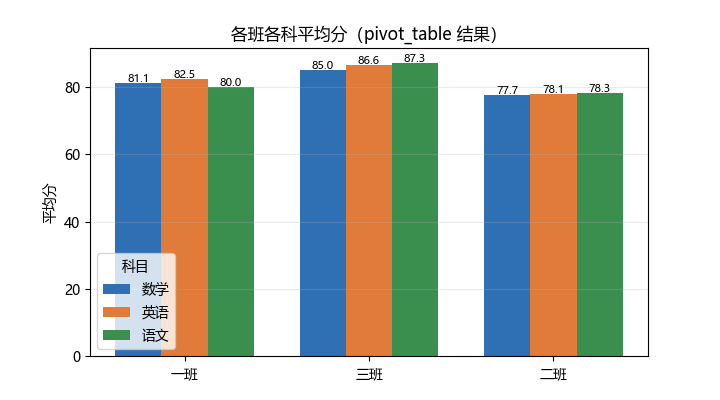
\includegraphics[keepaspectratio,alt={各班各科平均分}]{figures/04-pandas/case_scores.png}}
\caption{各班各科平均分}
\end{figure}

绘图代码：

\begin{Shaded}
\begin{Highlighting}[]
\ImportTok{import}\NormalTok{ matplotlib.pyplot }\ImportTok{as}\NormalTok{ plt}
\NormalTok{plt.rcParams[}\StringTok{\textquotesingle{}font.sans{-}serif\textquotesingle{}}\NormalTok{] }\OperatorTok{=}\NormalTok{ [}\StringTok{\textquotesingle{}Microsoft YaHei\textquotesingle{}}\NormalTok{, }\StringTok{\textquotesingle{}SimHei\textquotesingle{}}\NormalTok{, }\StringTok{\textquotesingle{}DejaVu Sans\textquotesingle{}}\NormalTok{]}
\NormalTok{plt.rcParams[}\StringTok{\textquotesingle{}axes.unicode\_minus\textquotesingle{}}\NormalTok{] }\OperatorTok{=} \VariableTok{False}

\NormalTok{fig, ax }\OperatorTok{=}\NormalTok{ plt.subplots(figsize}\OperatorTok{=}\NormalTok{(}\FloatTok{7.2}\NormalTok{, }\FloatTok{4.0}\NormalTok{))}
\NormalTok{subjects }\OperatorTok{=}\NormalTok{ piv.columns.tolist()}
\NormalTok{x }\OperatorTok{=}\NormalTok{ np.arange(}\BuiltInTok{len}\NormalTok{(piv.index))}
\NormalTok{colors }\OperatorTok{=}\NormalTok{ [}\StringTok{\textquotesingle{}\#2f6fb3\textquotesingle{}}\NormalTok{, }\StringTok{\textquotesingle{}\#e07b39\textquotesingle{}}\NormalTok{, }\StringTok{\textquotesingle{}\#3a8f4f\textquotesingle{}}\NormalTok{]}
\ControlFlowTok{for}\NormalTok{ j, sub }\KeywordTok{in} \BuiltInTok{enumerate}\NormalTok{(subjects):}
\NormalTok{    vals }\OperatorTok{=}\NormalTok{ piv[sub].values}
\NormalTok{    ax.bar(x }\OperatorTok{+}\NormalTok{ (j }\OperatorTok{{-}} \DecValTok{1}\NormalTok{) }\OperatorTok{*} \FloatTok{0.25}\NormalTok{, vals, width}\OperatorTok{=}\FloatTok{0.25}\NormalTok{, label}\OperatorTok{=}\NormalTok{sub, color}\OperatorTok{=}\NormalTok{colors[j])}
    \ControlFlowTok{for}\NormalTok{ xi, v }\KeywordTok{in} \BuiltInTok{zip}\NormalTok{(x }\OperatorTok{+}\NormalTok{ (j }\OperatorTok{{-}} \DecValTok{1}\NormalTok{) }\OperatorTok{*} \FloatTok{0.25}\NormalTok{, vals):}
\NormalTok{        ax.text(xi, v }\OperatorTok{+} \FloatTok{0.3}\NormalTok{, }\SpecialStringTok{f\textquotesingle{}}\SpecialCharTok{\{}\NormalTok{v}\SpecialCharTok{:.1f\}}\SpecialStringTok{\textquotesingle{}}\NormalTok{, ha}\OperatorTok{=}\StringTok{\textquotesingle{}center\textquotesingle{}}\NormalTok{, fontsize}\OperatorTok{=}\DecValTok{8}\NormalTok{)}
\NormalTok{ax.set\_xticks(x)}
\NormalTok{ax.set\_xticklabels(piv.index)}
\NormalTok{ax.set\_ylabel(}\StringTok{\textquotesingle{}平均分\textquotesingle{}}\NormalTok{)}
\NormalTok{ax.set\_title(}\StringTok{\textquotesingle{}各班各科平均分（pivot\_table 结果）\textquotesingle{}}\NormalTok{)}
\NormalTok{ax.legend(title}\OperatorTok{=}\StringTok{\textquotesingle{}科目\textquotesingle{}}\NormalTok{)}
\NormalTok{ax.grid(axis}\OperatorTok{=}\StringTok{\textquotesingle{}y\textquotesingle{}}\NormalTok{, alpha}\OperatorTok{=}\FloatTok{0.25}\NormalTok{)}
\NormalTok{fig.savefig(}\StringTok{\textquotesingle{}figures/04{-}pandas/case\_scores.png\textquotesingle{}}\NormalTok{)}
\NormalTok{plt.close(fig)}
\end{Highlighting}
\end{Shaded}

\subsubsection{4.2
各班成绩分布直方图}\label{ux5404ux73edux6210ux7ee9ux5206ux5e03ux76f4ux65b9ux56fe}

\begin{figure}
\centering
\pandocbounded{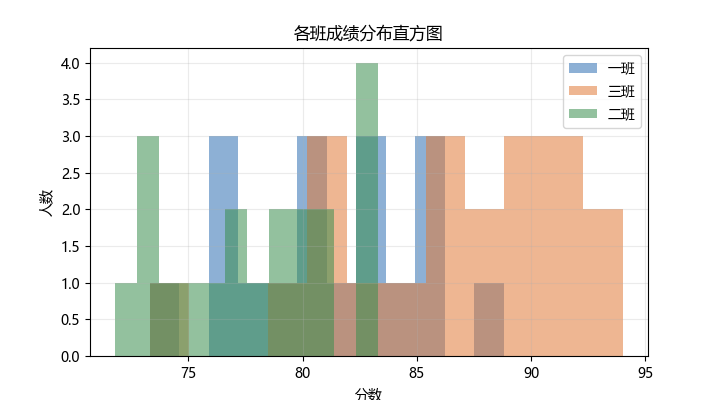
\includegraphics[keepaspectratio,alt={各班成绩分布}]{figures/04-pandas/case_distribution.png}}
\caption{各班成绩分布}
\end{figure}

\begin{Shaded}
\begin{Highlighting}[]
\NormalTok{fig, ax }\OperatorTok{=}\NormalTok{ plt.subplots(figsize}\OperatorTok{=}\NormalTok{(}\FloatTok{7.2}\NormalTok{, }\FloatTok{4.0}\NormalTok{))}
\ControlFlowTok{for}\NormalTok{ (cls, g), c }\KeywordTok{in} \BuiltInTok{zip}\NormalTok{(df.groupby(}\StringTok{\textquotesingle{}班级\textquotesingle{}}\NormalTok{), colors):}
\NormalTok{    ax.hist(g[}\StringTok{\textquotesingle{}分数\textquotesingle{}}\NormalTok{], bins}\OperatorTok{=}\DecValTok{12}\NormalTok{, alpha}\OperatorTok{=}\FloatTok{0.55}\NormalTok{, label}\OperatorTok{=}\NormalTok{cls, color}\OperatorTok{=}\NormalTok{c)}
\NormalTok{ax.set\_xlabel(}\StringTok{\textquotesingle{}分数\textquotesingle{}}\NormalTok{)}
\NormalTok{ax.set\_ylabel(}\StringTok{\textquotesingle{}人数\textquotesingle{}}\NormalTok{)}
\NormalTok{ax.set\_title(}\StringTok{\textquotesingle{}各班成绩分布直方图\textquotesingle{}}\NormalTok{)}
\NormalTok{ax.legend()}
\NormalTok{ax.grid(alpha}\OperatorTok{=}\FloatTok{0.25}\NormalTok{)}
\NormalTok{fig.savefig(}\StringTok{\textquotesingle{}figures/04{-}pandas/case\_distribution.png\textquotesingle{}}\NormalTok{)}
\NormalTok{plt.close(fig)}
\end{Highlighting}
\end{Shaded}

\subsubsection{4.3 时间序列：日到课人数 →
周均与移动平均}\label{ux65f6ux95f4ux5e8fux5217ux65e5ux5230ux8bfeux4ebaux6570-ux5468ux5747ux4e0eux79fbux52a8ux5e73ux5747}

\begin{figure}
\centering
\pandocbounded{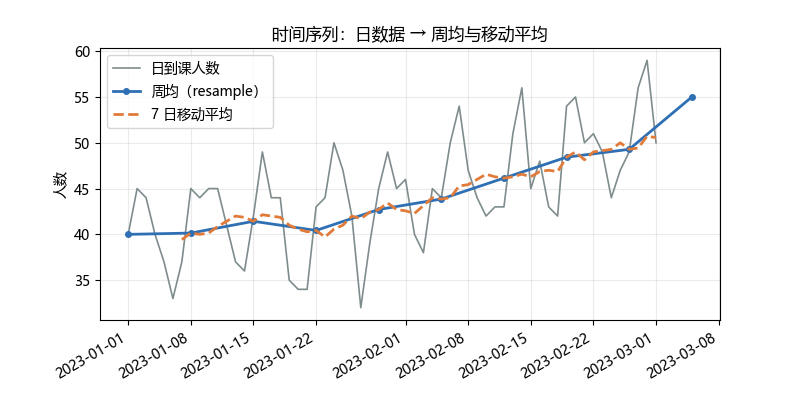
\includegraphics[keepaspectratio,alt={时间序列}]{figures/04-pandas/case_time_series.png}}
\caption{时间序列}
\end{figure}

\begin{Shaded}
\begin{Highlighting}[]
\NormalTok{rng }\OperatorTok{=}\NormalTok{ np.random.default\_rng(}\DecValTok{7}\NormalTok{)}
\NormalTok{idx }\OperatorTok{=}\NormalTok{ pd.date\_range(}\StringTok{\textquotesingle{}2023{-}01{-}01\textquotesingle{}}\NormalTok{, periods}\OperatorTok{=}\DecValTok{60}\NormalTok{, freq}\OperatorTok{=}\StringTok{\textquotesingle{}D\textquotesingle{}}\NormalTok{)}
\NormalTok{trend }\OperatorTok{=}\NormalTok{ np.linspace(}\DecValTok{0}\NormalTok{, }\DecValTok{10}\NormalTok{, }\DecValTok{60}\NormalTok{)}
\NormalTok{weekly }\OperatorTok{=} \DecValTok{5} \OperatorTok{*}\NormalTok{ np.sin(}\DecValTok{2} \OperatorTok{*}\NormalTok{ np.pi }\OperatorTok{*}\NormalTok{ np.arange(}\DecValTok{60}\NormalTok{) }\OperatorTok{/} \DecValTok{7}\NormalTok{)}
\NormalTok{count }\OperatorTok{=}\NormalTok{ (}\DecValTok{40} \OperatorTok{+}\NormalTok{ trend }\OperatorTok{+}\NormalTok{ weekly }\OperatorTok{+}\NormalTok{ rng.normal(}\DecValTok{0}\NormalTok{, }\DecValTok{3}\NormalTok{, }\DecValTok{60}\NormalTok{)).}\BuiltInTok{round}\NormalTok{().clip(}\DecValTok{0}\NormalTok{, }\DecValTok{60}\NormalTok{).astype(}\BuiltInTok{int}\NormalTok{)}
\NormalTok{ts }\OperatorTok{=}\NormalTok{ pd.Series(count, index}\OperatorTok{=}\NormalTok{idx)}
\NormalTok{weekly\_mean }\OperatorTok{=}\NormalTok{ ts.resample(}\StringTok{\textquotesingle{}W\textquotesingle{}}\NormalTok{).mean()}
\NormalTok{rolling7 }\OperatorTok{=}\NormalTok{ ts.rolling(}\DecValTok{7}\NormalTok{).mean()}

\NormalTok{fig, ax }\OperatorTok{=}\NormalTok{ plt.subplots(figsize}\OperatorTok{=}\NormalTok{(}\FloatTok{8.0}\NormalTok{, }\FloatTok{4.0}\NormalTok{))}
\NormalTok{ax.plot(ts.index, ts.values, color}\OperatorTok{=}\StringTok{\textquotesingle{}\#7f8c8d\textquotesingle{}}\NormalTok{, lw}\OperatorTok{=}\FloatTok{1.2}\NormalTok{, label}\OperatorTok{=}\StringTok{\textquotesingle{}日到课人数\textquotesingle{}}\NormalTok{)}
\NormalTok{ax.plot(weekly\_mean.index, weekly\_mean.values, color}\OperatorTok{=}\StringTok{\textquotesingle{}\#2f6fb3\textquotesingle{}}\NormalTok{, marker}\OperatorTok{=}\StringTok{\textquotesingle{}o\textquotesingle{}}\NormalTok{, ms}\OperatorTok{=}\DecValTok{4}\NormalTok{,}
\NormalTok{        lw}\OperatorTok{=}\DecValTok{2}\NormalTok{, label}\OperatorTok{=}\StringTok{\textquotesingle{}周均（resample）\textquotesingle{}}\NormalTok{)}
\NormalTok{ax.plot(rolling7.index, rolling7.values, color}\OperatorTok{=}\StringTok{\textquotesingle{}\#e07b39\textquotesingle{}}\NormalTok{, lw}\OperatorTok{=}\DecValTok{2}\NormalTok{, ls}\OperatorTok{=}\StringTok{\textquotesingle{}{-}{-}\textquotesingle{}}\NormalTok{, label}\OperatorTok{=}\StringTok{\textquotesingle{}7 日移动平均\textquotesingle{}}\NormalTok{)}
\NormalTok{ax.set\_ylabel(}\StringTok{\textquotesingle{}人数\textquotesingle{}}\NormalTok{)}
\NormalTok{ax.set\_title(}\StringTok{\textquotesingle{}时间序列：日数据 → 周均与移动平均\textquotesingle{}}\NormalTok{)}
\NormalTok{ax.legend()}
\NormalTok{ax.grid(alpha}\OperatorTok{=}\FloatTok{0.25}\NormalTok{)}
\NormalTok{fig.autofmt\_xdate()}
\NormalTok{fig.savefig(}\StringTok{\textquotesingle{}figures/04{-}pandas/case\_time\_series.png\textquotesingle{}}\NormalTok{)}
\NormalTok{plt.close(fig)}
\end{Highlighting}
\end{Shaded}

\subsection{5. 结论}\label{ux7ed3ux8bba}

\begin{itemize}
\tightlist
\item
  清洗后共 58 条有效记录，去掉 2 个缺失、1 行重复，并用 IQR 替换了 1
  个异常低分；
\item
  三班平均分最高（86.3），二班最低（78.0），这与我们设定的``班级基础分''一致；
\item
  透视表给出``班级 × 科目''的平均分，能快速定位薄弱科目；
\item
  时间序列图说明：\texttt{resample(\textquotesingle{}W\textquotesingle{})}
  把日数据聚合成周均，\texttt{rolling(7)} 得到平滑的 7
  日移动平均，二者都可用于观察趋势。
\end{itemize}

\subsection{拓展任务}\label{ux62d3ux5c55ux4efbux52a1-6}

\begin{enumerate}
\def\labelenumi{\arabic{enumi}.}
\tightlist
\item
  改用真实 CSV（如某课程成绩表）复现；
\item
  把
  \texttt{groupby(\textquotesingle{}班级\textquotesingle{}){[}\textquotesingle{}分数\textquotesingle{}{]}.agg({[}\textquotesingle{}mean\textquotesingle{},\ \textquotesingle{}std\textquotesingle{},\ \textquotesingle{}count\textquotesingle{}{]})}
  的结果也画成条形图；
\item
  对透视表加 \texttt{margins=True} 显示总计；
\item
  给时间序列数据加周末标记，观察周末到课人数是否更低。
\end{enumerate}

\subsection{延伸阅读}\label{ux5ef6ux4f38ux9605ux8bfb-19}

\begin{itemize}
\tightlist
\item
  Pandas
  分组与聚合文档：https://pandas.pydata.org/docs/user\_guide/groupby.html
\item
  Pandas
  透视表文档：https://pandas.pydata.org/docs/reference/api/pandas.pivot\_table.html
\item
  Pandas
  时间序列文档：https://pandas.pydata.org/docs/user\_guide/timeseries.html
\item
  Matplotlib
  官方入门：https://matplotlib.org/stable/tutorials/introductory/quick\_start.html
\end{itemize}

\section{04
常见误区与技巧}\label{ux5e38ux89c1ux8befux533aux4e0eux6280ux5de7-3}

\begin{quote}
本章为新增``查漏补缺''页：把学生最容易踩的坑集中列出，并给出正确的写法和性能/调试建议。
\end{quote}

\subsection{1.
高频误区速查表}\label{ux9ad8ux9891ux8befux533aux901fux67e5ux8868-3}

{\def\LTcaptype{none} % do not increment counter
\begin{longtable}[]{@{}
  >{\raggedright\arraybackslash}p{(\linewidth - 6\tabcolsep) * \real{0.2500}}
  >{\raggedright\arraybackslash}p{(\linewidth - 6\tabcolsep) * \real{0.2500}}
  >{\raggedright\arraybackslash}p{(\linewidth - 6\tabcolsep) * \real{0.2500}}
  >{\raggedright\arraybackslash}p{(\linewidth - 6\tabcolsep) * \real{0.2500}}@{}}
\toprule\noalign{}
\begin{minipage}[b]{\linewidth}\raggedright
\#
\end{minipage} & \begin{minipage}[b]{\linewidth}\raggedright
误区 / 错误写法
\end{minipage} & \begin{minipage}[b]{\linewidth}\raggedright
正确做法
\end{minipage} & \begin{minipage}[b]{\linewidth}\raggedright
原因
\end{minipage} \\
\midrule\noalign{}
\endhead
\bottomrule\noalign{}
\endlastfoot
1 & \texttt{df.loc{[}0{]}} 想取第一行但索引是字符串 &
\texttt{df.iloc{[}0{]}}（位置）或
\texttt{df.loc{[}\textquotesingle{}r0\textquotesingle{}{]}}（标签） &
loc 按标签、iloc 按位置 \\
2 & \texttt{s{[}0{]}} 取 Series 位置 & \texttt{s.iloc{[}0{]}} &
整数标签歧义，位置访问应显式 iloc \\
3 & \texttt{df{[}(df.A\textgreater{}2)\ and\ (df.B\textless{}40){]}} &
\texttt{df{[}(df.A\textgreater{}2)\ \&\ (df.B\textless{}40){]}}（每个条件加括号）
& \texttt{and}/\texttt{or} 用于 Python
布尔，\texttt{\&}/\texttt{\textbar{}} 用于逐元素布尔数组 \\
4 & \texttt{df{[}\textquotesingle{}A\textquotesingle{}{]}} 当``单个
DataFrame'' & 需要单列 DataFrame 用
\texttt{df{[}{[}\textquotesingle{}A\textquotesingle{}{]}{]}} &
\texttt{df{[}\textquotesingle{}A\textquotesingle{}{]}} 返回 Series \\
5 & \texttt{fillna(method=\textquotesingle{}ffill\textquotesingle{})} &
\texttt{df.ffill()} & pandas 2.x 已弃用 method 写法 \\
6 & \texttt{dropna()} 误删有效数据 & 先 \texttt{df.isna().sum()}
看缺失情况，用 \texttt{thresh} 控制 & dropna 默认删任意含缺失的行 \\
7 & 以为 \texttt{groupby} 返回 DataFrame & 返回 \texttt{groupby}
对象，需 \texttt{.mean()}/\texttt{.agg()} 等 & groupby 是``中间对象'' \\
8 & \texttt{pivot\_table} 出现 NaN & 加 \texttt{fill\_value=0} &
交叉格无数据 \\
9 & \texttt{resample(\textquotesingle{}W\textquotesingle{})}
当``滑动平均'' & 降频聚合用 resample；滑窗用 \texttt{rolling(7).mean()}
& 二者语义不同 \\
10 & 用 \texttt{apply} 做可向量化运算 & \texttt{s*2+1} 优先 & apply 逐行
Python 调用，慢 \\
11 & 修改切片后以为原数据不变 & 注意 Pandas
的视图/拷贝语义（建议对新结果 \texttt{.copy()}） & 部分切片是视图 \\
12 & 读 Excel 报错 & 先 \texttt{pip\ install\ openpyxl} & 缺读写引擎 \\
\end{longtable}
}

\subsection{2. 原理级难点：loc vs
iloc}\label{ux539fux7406ux7ea7ux96beux70b9loc-vs-iloc}

\begin{Shaded}
\begin{Highlighting}[]
\NormalTok{s }\OperatorTok{=}\NormalTok{ pd.Series([}\DecValTok{10}\NormalTok{, }\DecValTok{20}\NormalTok{, }\DecValTok{30}\NormalTok{], index}\OperatorTok{=}\NormalTok{[}\StringTok{\textquotesingle{}a\textquotesingle{}}\NormalTok{, }\StringTok{\textquotesingle{}b\textquotesingle{}}\NormalTok{, }\StringTok{\textquotesingle{}c\textquotesingle{}}\NormalTok{])}
\BuiltInTok{print}\NormalTok{(s.loc[}\StringTok{\textquotesingle{}b\textquotesingle{}}\NormalTok{])     }\CommentTok{\# 20（按标签）}
\BuiltInTok{print}\NormalTok{(s.iloc[}\DecValTok{1}\NormalTok{])      }\CommentTok{\# 20（按位置）}
\end{Highlighting}
\end{Shaded}

\begin{itemize}
\tightlist
\item
  标签是字符串时，\texttt{s{[}0{]}} 会歧义甚至报错；统一
  \texttt{s.loc{[}\textquotesingle{}b\textquotesingle{}{]}} /
  \texttt{s.iloc{[}1{]}}。
\item
  \texttt{.loc}
  切片是\textbf{闭区间}（\texttt{df.loc{[}\textquotesingle{}a\textquotesingle{}:\textquotesingle{}c\textquotesingle{}{]}}
  含 c），\texttt{.iloc}
  切片是\textbf{开区间}（\texttt{df.iloc{[}0:2{]}} 只含 0,1）。
\end{itemize}

\subsection{3. 性能技巧}\label{ux6027ux80fdux6280ux5de7-3}

\begin{itemize}
\tightlist
\item
  \textbf{向量化优先}：能
  \texttt{df{[}\textquotesingle{}x\textquotesingle{}{]}\ *\ 2\ +\ 1}
  就不要
  \texttt{df{[}\textquotesingle{}x\textquotesingle{}{]}.apply(lambda\ v:\ v*2+1)}；
\item
  \textbf{避免在循环里逐行
  \texttt{append}/\texttt{concat}}：先用列表收集再一次性
  \texttt{pd.DataFrame(...)}；
\item
  \textbf{用 \texttt{rename}/\texttt{astype}
  前先想好副本}：多数方法返回新对象；
\item
  \textbf{大文件用
  \texttt{chunksize}}：\texttt{pd.read\_csv(\textquotesingle{}big.csv\textquotesingle{},\ chunksize=10\_000)}
  分批读；
\item
  \textbf{时间序列避免逐元素循环}：用
  \texttt{resample}/\texttt{rolling}/\texttt{shift}/\texttt{diff}；
\item
  \textbf{用 \texttt{pd.qcut}/\texttt{cut}} 做分箱，避免手写条件判断。
\end{itemize}

\subsection{4. 调试建议}\label{ux8c03ux8bd5ux5efaux8bae-3}

\begin{enumerate}
\def\labelenumi{\arabic{enumi}.}
\tightlist
\item
  先打印 \texttt{df.head()}、\texttt{df.dtypes}、\texttt{df.shape}
  确认数据形状；
\item
  布尔筛选把中间掩码存成变量：\texttt{mask\ =\ (df.A\ \textgreater{}\ 2)\ \&\ (df.B\ \textless{}\ 40);\ df{[}mask{]}}；
\item
  用 \texttt{df.isna().sum()} 检查缺失；用
  \texttt{df.duplicated().sum()} 检查重复；
\item
  遇到 \texttt{KeyError} 先打印 \texttt{df.columns}；
\item
  数值异常用 \texttt{df.describe()} 看 min/max/分位数；
\item
  随机/抽样问题\textbf{固定种子}
  \texttt{rng\ =\ np.random.default\_rng(42)}。
\end{enumerate}

\subsection{5.
本章小结（自测清单）}\label{ux672cux7ae0ux5c0fux7ed3ux81eaux6d4bux6e05ux5355}

\begin{itemize}
\tightlist
\item[$\square$]
  能解释 Series 与 DataFrame 的区别；
\item[$\square$]
  能说出 \texttt{.loc} 与 \texttt{.iloc} 的三个不同点；
\item[$\square$]
  会写 \texttt{df{[}(df.A\textgreater{}2)\ \&\ (df.B\textless{}40){]}}
  的多条件布尔筛选；
\item[$\square$]
  会用
  \texttt{drop\_duplicates}/\texttt{fillna}/\texttt{dropna}/\texttt{ffill}
  清数据；
\item[$\square$]
  会用 IQR 找异常并替换；
\item[$\square$]
  会做 Min-Max 与 Z-Score，并说出适用场景；
\item[$\square$]
  会 \texttt{groupby}/\texttt{pivot\_table} 做分组透视；
\item[$\square$]
  会 \texttt{resample}/\texttt{rolling} 处理时间序列；
\item[$\square$]
  会画 matplotlib 图（中文字体）并生成案例配图。
\end{itemize}

\subsection{延伸阅读}\label{ux5ef6ux4f38ux9605ux8bfb-20}

\begin{itemize}
\tightlist
\item
  Pandas
  官方``用户指南''：https://pandas.pydata.org/docs/user\_guide/index.html
\item
  Pandas
  官方``性能提升''：https://pandas.pydata.org/docs/user\_guide/enhancingperf.html
\item
  Python Data Science Handbook（第 3 章
  Pandas）：https://github.com/jakevdp/PythonDataScienceHandbook
\end{itemize}

\newpage

%% 由 build/emit_tex.py 生成（生成物，勿手改）；定制请放 user_style.tex / user_meta.yaml
\chapter{Matplotlib及其基本使用}\label{matplotlibux53caux5176ux57faux672cux4f7fux7528}

\section{01
基本绘图：折线、散点、条形、饼图、直方图、箱线图等}\label{ux57faux672cux7ed8ux56feux6298ux7ebfux6563ux70b9ux6761ux5f62ux997cux56feux76f4ux65b9ux56feux7bb1ux7ebfux56feux7b49}

\begin{quote}
本节对应原版 5.1 的内容，并增补学习目标、常见误区、思考题与延伸阅读。
配套图：\texttt{figures/05-matplotlib/basic\_plots.png}（由
\texttt{build/make\_chap5\_figures.py} 生成）。
\end{quote}

\subsection{本节目标}\label{ux672cux8282ux76eeux6807-13}

\begin{itemize}
\tightlist
\item
  会用 \texttt{matplotlib.pyplot} 绘制 6 种最常用的基础图表；
\item
  理解面向对象接口（\texttt{fig} /
  \texttt{ax}）与``函数式''接口（\texttt{plt.plot}）的关系；
\item
  会为图表添加标题、坐标轴标签、图例；
\item
  接触热力图、误差棒图、极坐标、3D、等高线等扩展图型。
\end{itemize}

\subsection{先修}\label{ux5148ux4fee-13}

\begin{itemize}
\tightlist
\item
  Python 基础语法；NumPy
  数组（\texttt{np.linspace}、\texttt{np.arange}、随机数）。
\end{itemize}

\subsection{官方文档/参考入口}\label{ux5b98ux65b9ux6587ux6863ux53c2ux8003ux5165ux53e3-2}

\begin{itemize}
\tightlist
\item
  Matplotlib
  官方快速开始：https://matplotlib.org/stable/tutorials/introductory/quick\_start.html
\item
  Matplotlib 图型画廊：https://matplotlib.org/stable/gallery/index.html
\end{itemize}

\begin{center}\rule{0.5\linewidth}{0.5pt}\end{center}

\subsection{\texorpdfstring{1.1
快速开始：\texttt{import\ matplotlib.pyplot\ as\ plt}}{1.1 快速开始：import matplotlib.pyplot as plt}}\label{ux5febux901fux5f00ux59cbimport-matplotlib.pyplot-as-plt}

\begin{quote}
Matplotlib
有两种风格：\textbf{函数式}（\texttt{plt.plot}，自动管理当前图）与\textbf{面向对象}（\texttt{fig,\ ax\ =\ plt.subplots()}，手动管理
Axes）。本教材优先介绍函数式，第 2 节再切换到面向对象。
\end{quote}

\begin{Shaded}
\begin{Highlighting}[]
\ImportTok{import}\NormalTok{ matplotlib.pyplot }\ImportTok{as}\NormalTok{ plt}

\NormalTok{x }\OperatorTok{=}\NormalTok{ [}\DecValTok{1}\NormalTok{, }\DecValTok{2}\NormalTok{, }\DecValTok{3}\NormalTok{, }\DecValTok{4}\NormalTok{, }\DecValTok{5}\NormalTok{]}
\NormalTok{y }\OperatorTok{=}\NormalTok{ [}\DecValTok{1}\NormalTok{, }\DecValTok{4}\NormalTok{, }\DecValTok{9}\NormalTok{, }\DecValTok{16}\NormalTok{, }\DecValTok{25}\NormalTok{]}

\NormalTok{plt.plot(x, y)}
\NormalTok{plt.title(}\StringTok{\textquotesingle{}Simple Plot\textquotesingle{}}\NormalTok{)}
\NormalTok{plt.xlabel(}\StringTok{\textquotesingle{}x axis\textquotesingle{}}\NormalTok{)}
\NormalTok{plt.ylabel(}\StringTok{\textquotesingle{}y axis\textquotesingle{}}\NormalTok{)}
\NormalTok{plt.show()}
\end{Highlighting}
\end{Shaded}

运行后得到一条折线。若在 Jupyter 中，\texttt{plt.show()}
会把图形显示在输出区；在脚本中则弹出窗口（无窗口环境请用
\texttt{plt.savefig}）。

\subsection{1.2
常见基础图表}\label{ux5e38ux89c1ux57faux7840ux56feux8868}

\subsubsection{\texorpdfstring{1.2.1
折线图（\texttt{plot}）}{1.2.1 折线图（plot）}}\label{ux6298ux7ebfux56feplot}

\begin{Shaded}
\begin{Highlighting}[]
\ImportTok{import}\NormalTok{ numpy }\ImportTok{as}\NormalTok{ np}
\ImportTok{import}\NormalTok{ matplotlib.pyplot }\ImportTok{as}\NormalTok{ plt}

\NormalTok{x }\OperatorTok{=}\NormalTok{ [}\DecValTok{1}\NormalTok{, }\DecValTok{2}\NormalTok{, }\DecValTok{3}\NormalTok{, }\DecValTok{4}\NormalTok{, }\DecValTok{5}\NormalTok{]}
\NormalTok{y }\OperatorTok{=}\NormalTok{ [}\DecValTok{1}\NormalTok{, }\DecValTok{4}\NormalTok{, }\DecValTok{9}\NormalTok{, }\DecValTok{16}\NormalTok{, }\DecValTok{25}\NormalTok{]}
\NormalTok{plt.plot(x, y)}
\NormalTok{plt.title(}\StringTok{\textquotesingle{}Simple Plot\textquotesingle{}}\NormalTok{)}
\NormalTok{plt.xlabel(}\StringTok{\textquotesingle{}x axis\textquotesingle{}}\NormalTok{)}
\NormalTok{plt.ylabel(}\StringTok{\textquotesingle{}y axis\textquotesingle{}}\NormalTok{)}
\BuiltInTok{print}\NormalTok{(}\StringTok{\textquotesingle{}x:\textquotesingle{}}\NormalTok{, x)}
\BuiltInTok{print}\NormalTok{(}\StringTok{\textquotesingle{}y:\textquotesingle{}}\NormalTok{, y)}
\end{Highlighting}
\end{Shaded}

\begin{Shaded}
\begin{Highlighting}[]
\NormalTok{x: [1, 2, 3, 4, 5]}
\NormalTok{y: [1, 4, 9, 16, 25]}
\end{Highlighting}
\end{Shaded}

\subsubsection{\texorpdfstring{1.2.2
散点图（\texttt{scatter}）}{1.2.2 散点图（scatter）}}\label{ux6563ux70b9ux56fescatter}

\begin{Shaded}
\begin{Highlighting}[]
\ImportTok{import}\NormalTok{ numpy }\ImportTok{as}\NormalTok{ np}
\ImportTok{import}\NormalTok{ matplotlib.pyplot }\ImportTok{as}\NormalTok{ plt}

\NormalTok{rng }\OperatorTok{=}\NormalTok{ np.random.default\_rng(}\DecValTok{0}\NormalTok{)}
\NormalTok{x }\OperatorTok{=}\NormalTok{ rng.normal(}\DecValTok{0}\NormalTok{, }\DecValTok{1}\NormalTok{, }\DecValTok{60}\NormalTok{)}
\NormalTok{y }\OperatorTok{=} \FloatTok{0.6} \OperatorTok{*}\NormalTok{ x }\OperatorTok{+}\NormalTok{ rng.normal(}\DecValTok{0}\NormalTok{, }\FloatTok{0.4}\NormalTok{, }\DecValTok{60}\NormalTok{)}
\NormalTok{plt.scatter(x, y, s}\OperatorTok{=}\DecValTok{28}\NormalTok{, c}\OperatorTok{=}\StringTok{\textquotesingle{}\#e07b39\textquotesingle{}}\NormalTok{, alpha}\OperatorTok{=}\FloatTok{0.8}\NormalTok{)}
\NormalTok{plt.title(}\StringTok{\textquotesingle{}Scatter Plot\textquotesingle{}}\NormalTok{)}
\BuiltInTok{print}\NormalTok{(}\StringTok{\textquotesingle{}x min/max:\textquotesingle{}}\NormalTok{, }\BuiltInTok{round}\NormalTok{(x.}\BuiltInTok{min}\NormalTok{(), }\DecValTok{3}\NormalTok{), }\BuiltInTok{round}\NormalTok{(x.}\BuiltInTok{max}\NormalTok{(), }\DecValTok{3}\NormalTok{))}
\BuiltInTok{print}\NormalTok{(}\StringTok{\textquotesingle{}y mean:\textquotesingle{}}\NormalTok{, }\BuiltInTok{round}\NormalTok{(y.mean(), }\DecValTok{3}\NormalTok{))}
\end{Highlighting}
\end{Shaded}

\begin{Shaded}
\begin{Highlighting}[]
\NormalTok{x min/max: {-}2.325 1.96}
\NormalTok{y mean: 0.08}
\end{Highlighting}
\end{Shaded}

\begin{quote}
\texttt{s} 控制点面积、\texttt{c} 控制颜色、\texttt{alpha}
控制透明度；\texttt{np.random.default\_rng(0)} 保证结果可复现。
\end{quote}

\subsubsection{\texorpdfstring{1.2.3
条形图（\texttt{bar}）}{1.2.3 条形图（bar）}}\label{ux6761ux5f62ux56febar}

\begin{Shaded}
\begin{Highlighting}[]
\ImportTok{import}\NormalTok{ matplotlib.pyplot }\ImportTok{as}\NormalTok{ plt}

\NormalTok{cats }\OperatorTok{=}\NormalTok{ [}\StringTok{\textquotesingle{}A\textquotesingle{}}\NormalTok{, }\StringTok{\textquotesingle{}B\textquotesingle{}}\NormalTok{, }\StringTok{\textquotesingle{}C\textquotesingle{}}\NormalTok{, }\StringTok{\textquotesingle{}D\textquotesingle{}}\NormalTok{]}
\NormalTok{vals }\OperatorTok{=}\NormalTok{ [}\DecValTok{23}\NormalTok{, }\DecValTok{45}\NormalTok{, }\DecValTok{56}\NormalTok{, }\DecValTok{78}\NormalTok{]}
\NormalTok{plt.bar(cats, vals)}
\NormalTok{plt.title(}\StringTok{\textquotesingle{}Bar Chart\textquotesingle{}}\NormalTok{)}
\NormalTok{plt.xlabel(}\StringTok{\textquotesingle{}Categories\textquotesingle{}}\NormalTok{)}
\NormalTok{plt.ylabel(}\StringTok{\textquotesingle{}Values\textquotesingle{}}\NormalTok{)}
\BuiltInTok{print}\NormalTok{(}\StringTok{\textquotesingle{}vals:\textquotesingle{}}\NormalTok{, vals)}
\BuiltInTok{print}\NormalTok{(}\StringTok{\textquotesingle{}total:\textquotesingle{}}\NormalTok{, }\BuiltInTok{sum}\NormalTok{(vals))}
\end{Highlighting}
\end{Shaded}

\begin{Shaded}
\begin{Highlighting}[]
\NormalTok{vals: [23, 45, 56, 78]}
\NormalTok{total: 202}
\end{Highlighting}
\end{Shaded}

\subsubsection{\texorpdfstring{1.2.4
饼图（\texttt{pie}）}{1.2.4 饼图（pie）}}\label{ux997cux56fepie}

\begin{Shaded}
\begin{Highlighting}[]
\ImportTok{import}\NormalTok{ matplotlib.pyplot }\ImportTok{as}\NormalTok{ plt}

\NormalTok{labels }\OperatorTok{=} \StringTok{\textquotesingle{}Frogs\textquotesingle{}}\NormalTok{, }\StringTok{\textquotesingle{}Hogs\textquotesingle{}}\NormalTok{, }\StringTok{\textquotesingle{}Dogs\textquotesingle{}}\NormalTok{, }\StringTok{\textquotesingle{}Logs\textquotesingle{}}
\NormalTok{sizes }\OperatorTok{=}\NormalTok{ [}\DecValTok{15}\NormalTok{, }\DecValTok{30}\NormalTok{, }\DecValTok{45}\NormalTok{, }\DecValTok{10}\NormalTok{]}
\NormalTok{plt.pie(sizes, labels}\OperatorTok{=}\NormalTok{labels, autopct}\OperatorTok{=}\StringTok{\textquotesingle{}}\SpecialCharTok{\%1.1f\%\%}\StringTok{\textquotesingle{}}\NormalTok{, startangle}\OperatorTok{=}\DecValTok{140}\NormalTok{)}
\NormalTok{plt.title(}\StringTok{\textquotesingle{}Pie Chart\textquotesingle{}}\NormalTok{)}
\NormalTok{plt.axis(}\StringTok{\textquotesingle{}equal\textquotesingle{}}\NormalTok{)}
\BuiltInTok{print}\NormalTok{(}\StringTok{\textquotesingle{}sizes:\textquotesingle{}}\NormalTok{, sizes, }\StringTok{\textquotesingle{}sum:\textquotesingle{}}\NormalTok{, }\BuiltInTok{sum}\NormalTok{(sizes))}
\end{Highlighting}
\end{Shaded}

\begin{Shaded}
\begin{Highlighting}[]
\NormalTok{sizes: [15, 30, 45, 10] sum: 100}
\end{Highlighting}
\end{Shaded}

\begin{quote}
\texttt{autopct} 控制百分比格式，\texttt{startangle}
控制起始角度，\texttt{axis(\textquotesingle{}equal\textquotesingle{})}
保证饼图是正圆。
\end{quote}

\subsubsection{\texorpdfstring{1.2.5
直方图（\texttt{hist}）}{1.2.5 直方图（hist）}}\label{ux76f4ux65b9ux56fehist}

\begin{Shaded}
\begin{Highlighting}[]
\ImportTok{import}\NormalTok{ numpy }\ImportTok{as}\NormalTok{ np}
\ImportTok{import}\NormalTok{ matplotlib.pyplot }\ImportTok{as}\NormalTok{ plt}

\NormalTok{mu, sigma }\OperatorTok{=} \DecValTok{0}\NormalTok{, }\FloatTok{0.1}
\NormalTok{data }\OperatorTok{=}\NormalTok{ np.random.default\_rng(}\DecValTok{5}\NormalTok{).normal(mu, sigma, }\DecValTok{1000}\NormalTok{)}
\NormalTok{counts, bins, patches }\OperatorTok{=}\NormalTok{ plt.hist(data, bins}\OperatorTok{=}\DecValTok{30}\NormalTok{, density}\OperatorTok{=}\VariableTok{True}\NormalTok{)}
\NormalTok{plt.title(}\StringTok{\textquotesingle{}Histogram\textquotesingle{}}\NormalTok{)}
\NormalTok{plt.xlabel(}\StringTok{\textquotesingle{}Value\textquotesingle{}}\NormalTok{)}
\NormalTok{plt.ylabel(}\StringTok{\textquotesingle{}Frequency\textquotesingle{}}\NormalTok{)}
\BuiltInTok{print}\NormalTok{(}\StringTok{\textquotesingle{}bin count:\textquotesingle{}}\NormalTok{, }\BuiltInTok{len}\NormalTok{(patches))}
\BuiltInTok{print}\NormalTok{(}\StringTok{\textquotesingle{}first/last bin:\textquotesingle{}}\NormalTok{, }\BuiltInTok{round}\NormalTok{(bins[}\DecValTok{0}\NormalTok{], }\DecValTok{3}\NormalTok{), }\BuiltInTok{round}\NormalTok{(bins[}\OperatorTok{{-}}\DecValTok{1}\NormalTok{], }\DecValTok{3}\NormalTok{))}
\end{Highlighting}
\end{Shaded}

\begin{Shaded}
\begin{Highlighting}[]
\NormalTok{bin count: 30}
\NormalTok{first/last bin: {-}0.328 0.311}
\end{Highlighting}
\end{Shaded}

\begin{quote}
\texttt{density=True} 时纵轴是概率密度（面积归一为 1）；\texttt{bins}
为分箱数。
\end{quote}

\subsubsection{\texorpdfstring{1.2.6
箱线图（\texttt{boxplot}）}{1.2.6 箱线图（boxplot）}}\label{ux7bb1ux7ebfux56feboxplot}

\begin{Shaded}
\begin{Highlighting}[]
\ImportTok{import}\NormalTok{ numpy }\ImportTok{as}\NormalTok{ np}
\ImportTok{import}\NormalTok{ matplotlib.pyplot }\ImportTok{as}\NormalTok{ plt}

\NormalTok{np.random.seed(}\DecValTok{10}\NormalTok{)}
\NormalTok{data }\OperatorTok{=}\NormalTok{ np.random.normal(}\DecValTok{0}\NormalTok{, }\DecValTok{1}\NormalTok{, }\DecValTok{200}\NormalTok{)}
\NormalTok{data }\OperatorTok{=}\NormalTok{ np.concatenate([data, [}\DecValTok{10}\NormalTok{]])   }\CommentTok{\# 加入一个异常值}
\NormalTok{plt.boxplot(data)}
\NormalTok{plt.title(}\StringTok{\textquotesingle{}Boxplot\textquotesingle{}}\NormalTok{)}
\BuiltInTok{print}\NormalTok{(}\StringTok{\textquotesingle{}outliers \textgreater{} 3:\textquotesingle{}}\NormalTok{, }\BuiltInTok{int}\NormalTok{((data }\OperatorTok{\textgreater{}} \DecValTok{3}\NormalTok{).}\BuiltInTok{sum}\NormalTok{()))}
\BuiltInTok{print}\NormalTok{(}\StringTok{\textquotesingle{}max:\textquotesingle{}}\NormalTok{, }\BuiltInTok{round}\NormalTok{(data.}\BuiltInTok{max}\NormalTok{(), }\DecValTok{2}\NormalTok{))}
\end{Highlighting}
\end{Shaded}

\begin{Shaded}
\begin{Highlighting}[]
\NormalTok{outliers \textgreater{} 3: 1}
\NormalTok{max: 10.0}
\end{Highlighting}
\end{Shaded}

\begin{quote}
箱线图用五数概括（Q1、中位数、Q3、上下须）展示分布，异常值以离群点显示。
\end{quote}

\subsubsection{\texorpdfstring{1.2.7
热力图（\texttt{imshow}）}{1.2.7 热力图（imshow）}}\label{ux70edux529bux56feimshow}

\begin{Shaded}
\begin{Highlighting}[]
\ImportTok{import}\NormalTok{ numpy }\ImportTok{as}\NormalTok{ np}
\ImportTok{import}\NormalTok{ matplotlib.pyplot }\ImportTok{as}\NormalTok{ plt}

\NormalTok{data }\OperatorTok{=}\NormalTok{ np.random.default\_rng(}\DecValTok{7}\NormalTok{).random((}\DecValTok{10}\NormalTok{, }\DecValTok{10}\NormalTok{))}
\NormalTok{plt.imshow(data, cmap}\OperatorTok{=}\StringTok{\textquotesingle{}hot\textquotesingle{}}\NormalTok{, interpolation}\OperatorTok{=}\StringTok{\textquotesingle{}nearest\textquotesingle{}}\NormalTok{)}
\NormalTok{plt.colorbar()}
\NormalTok{plt.title(}\StringTok{\textquotesingle{}Heatmap Example\textquotesingle{}}\NormalTok{)}
\BuiltInTok{print}\NormalTok{(}\StringTok{\textquotesingle{}matrix shape:\textquotesingle{}}\NormalTok{, data.shape)}
\end{Highlighting}
\end{Shaded}

\begin{Shaded}
\begin{Highlighting}[]
\NormalTok{matrix shape: (10, 10)}
\end{Highlighting}
\end{Shaded}

\begin{quote}
\texttt{imshow} 适合展示 2D 数值矩阵；\texttt{cmap}
控制配色，\texttt{colorbar} 加色标。
\end{quote}

\subsubsection{\texorpdfstring{1.2.8
误差棒图（\texttt{errorbar}）}{1.2.8 误差棒图（errorbar）}}\label{ux8befux5deeux68d2ux56feerrorbar}

\begin{Shaded}
\begin{Highlighting}[]
\ImportTok{import}\NormalTok{ numpy }\ImportTok{as}\NormalTok{ np}
\ImportTok{import}\NormalTok{ matplotlib.pyplot }\ImportTok{as}\NormalTok{ plt}

\NormalTok{x }\OperatorTok{=}\NormalTok{ np.arange(}\FloatTok{0.1}\NormalTok{, }\DecValTok{4}\NormalTok{, }\FloatTok{0.5}\NormalTok{)}
\NormalTok{y }\OperatorTok{=}\NormalTok{ np.exp(}\OperatorTok{{-}}\NormalTok{x)}
\NormalTok{yerr }\OperatorTok{=} \FloatTok{0.1} \OperatorTok{+} \FloatTok{0.2} \OperatorTok{*}\NormalTok{ np.sqrt(x)}
\NormalTok{xerr }\OperatorTok{=} \FloatTok{0.1} \OperatorTok{*}\NormalTok{ np.ones\_like(x)}
\NormalTok{plt.errorbar(x, y, xerr}\OperatorTok{=}\NormalTok{xerr, yerr}\OperatorTok{=}\NormalTok{yerr, fmt}\OperatorTok{=}\StringTok{\textquotesingle{}{-}o\textquotesingle{}}\NormalTok{)}
\NormalTok{plt.title(}\StringTok{\textquotesingle{}Errorbar Chart Example\textquotesingle{}}\NormalTok{)}
\BuiltInTok{print}\NormalTok{(}\StringTok{\textquotesingle{}n points:\textquotesingle{}}\NormalTok{, x.size)}
\end{Highlighting}
\end{Shaded}

\begin{Shaded}
\begin{Highlighting}[]
\NormalTok{n points: 8}
\end{Highlighting}
\end{Shaded}

\subsubsection{1.2.9
扩展图型：极坐标、3D、等高线}\label{ux6269ux5c55ux56feux578bux6781ux5750ux68073dux7b49ux9ad8ux7ebf}

\begin{Shaded}
\begin{Highlighting}[]
\ImportTok{import}\NormalTok{ numpy }\ImportTok{as}\NormalTok{ np}
\ImportTok{import}\NormalTok{ matplotlib.pyplot }\ImportTok{as}\NormalTok{ plt}
\ImportTok{from}\NormalTok{ mpl\_toolkits.mplot3d }\ImportTok{import}\NormalTok{ Axes3D}

\CommentTok{\#\# 极坐标}
\NormalTok{r }\OperatorTok{=}\NormalTok{ np.arange(}\DecValTok{0}\NormalTok{, }\DecValTok{2}\NormalTok{, }\FloatTok{0.01}\NormalTok{)}
\NormalTok{theta }\OperatorTok{=} \DecValTok{2} \OperatorTok{*}\NormalTok{ np.pi }\OperatorTok{*}\NormalTok{ r}
\NormalTok{plt.polar(theta, r)}
\NormalTok{plt.title(}\StringTok{\textquotesingle{}Polar Chart\textquotesingle{}}\NormalTok{)}
\BuiltInTok{print}\NormalTok{(}\StringTok{\textquotesingle{}polar points:\textquotesingle{}}\NormalTok{, r.size)}

\CommentTok{\#\# 3D 曲面}
\NormalTok{x }\OperatorTok{=}\NormalTok{ np.linspace(}\OperatorTok{{-}}\DecValTok{5}\NormalTok{, }\DecValTok{5}\NormalTok{, }\DecValTok{100}\NormalTok{)}\OperatorTok{;}\NormalTok{ y }\OperatorTok{=}\NormalTok{ np.linspace(}\OperatorTok{{-}}\DecValTok{5}\NormalTok{, }\DecValTok{5}\NormalTok{, }\DecValTok{100}\NormalTok{)}
\NormalTok{X, Y }\OperatorTok{=}\NormalTok{ np.meshgrid(x, y)}
\NormalTok{Z }\OperatorTok{=}\NormalTok{ np.sin(np.sqrt(X}\OperatorTok{**}\DecValTok{2} \OperatorTok{+}\NormalTok{ Y}\OperatorTok{**}\DecValTok{2}\NormalTok{))}
\NormalTok{fig }\OperatorTok{=}\NormalTok{ plt.figure()}
\NormalTok{ax }\OperatorTok{=}\NormalTok{ fig.add\_subplot(}\DecValTok{111}\NormalTok{, projection}\OperatorTok{=}\StringTok{\textquotesingle{}3d\textquotesingle{}}\NormalTok{)}
\NormalTok{ax.plot\_surface(X, Y, Z, cmap}\OperatorTok{=}\StringTok{\textquotesingle{}viridis\textquotesingle{}}\NormalTok{)}
\BuiltInTok{print}\NormalTok{(}\StringTok{\textquotesingle{}surface shape:\textquotesingle{}}\NormalTok{, Z.shape)}
\NormalTok{plt.close(fig)     }\CommentTok{\# 关闭 3D 图，避免与下面的等高线共用 Figure}

\CommentTok{\#\# 等高线}
\NormalTok{plt.contour(X, Y, Z, colors}\OperatorTok{=}\StringTok{\textquotesingle{}k\textquotesingle{}}\NormalTok{)}
\NormalTok{plt.contourf(X, Y, Z, cmap}\OperatorTok{=}\StringTok{\textquotesingle{}viridis\textquotesingle{}}\NormalTok{)}
\NormalTok{plt.colorbar()}
\BuiltInTok{print}\NormalTok{(}\StringTok{\textquotesingle{}X,Y,Z shapes:\textquotesingle{}}\NormalTok{, X.shape, Y.shape, Z.shape)}
\end{Highlighting}
\end{Shaded}

\begin{Shaded}
\begin{Highlighting}[]
\NormalTok{polar points: 200}
\NormalTok{surface shape: (100, 100)}
\NormalTok{X,Y,Z shapes: (100, 100) (100, 100) (100, 100)}
\end{Highlighting}
\end{Shaded}

\begin{quote}
3D 图需要
\texttt{from\ mpl\_toolkits.mplot3d\ import\ Axes3D}；\texttt{add\_subplot(111,\ projection=\textquotesingle{}3d\textquotesingle{})}
表示 1×1 网格中的第一个子图（详见第 2 节）。
\end{quote}

\begin{figure}
\centering
\pandocbounded{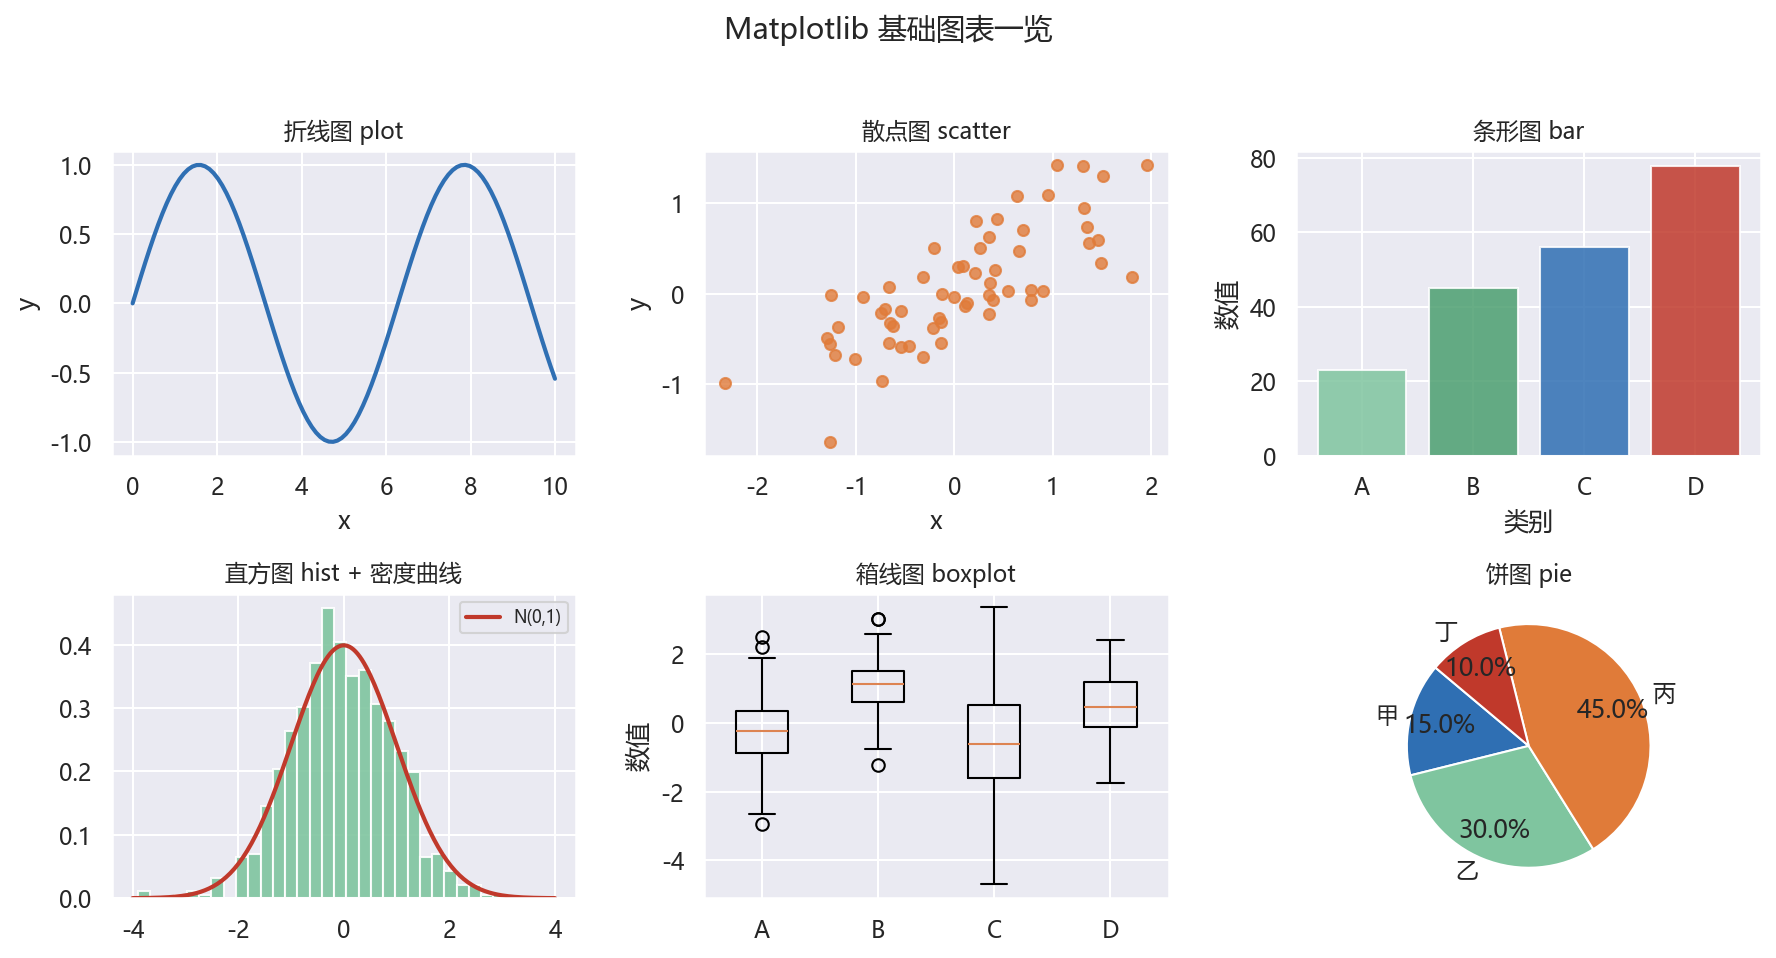
\includegraphics[keepaspectratio,alt={基础图表一览}]{figures/05-matplotlib/basic_plots.png}}
\caption{基础图表一览}
\end{figure}

\subsection{常见误区}\label{ux5e38ux89c1ux8befux533a-13}

\begin{enumerate}
\def\labelenumi{\arabic{enumi}.}
\tightlist
\item
  \textbf{只调用 \texttt{plt.plot} 不调用 \texttt{plt.show()} 或
  \texttt{savefig}}：在脚本中可能不显示也不保存，图形``消失''。
\item
  \textbf{对 \texttt{imshow} 不加
  \texttt{colorbar}}：看不出数值颜色映射。
\item
  \textbf{\texttt{plt.hist}
  直接打印可以拿到三个返回值}：\texttt{counts,\ bins,\ patches}，很多同学忽略。
\item
  \textbf{误以为 \texttt{pie} 的
  \texttt{axis(\textquotesingle{}equal\textquotesingle{})}
  可省}：不设会变成椭圆。
\item
  \textbf{随机数不设种子}：每次输出不同，课堂演示/作业请用
  \texttt{default\_rng(seed)}。
\end{enumerate}

\subsection{思考题}\label{ux601dux8003ux9898-13}

\begin{enumerate}
\def\labelenumi{\arabic{enumi}.}
\tightlist
\item
  为什么 \texttt{plt.plot(x,\ y)} 与
  \texttt{fig,\ ax\ =\ plt.subplots();\ ax.plot(x,\ y)}
  等价？它们分别管理什么状态？
\item
  \texttt{plt.scatter} 与
  \texttt{plt.plot(...,\ marker=\textquotesingle{}o\textquotesingle{})}
  对一维数据有何适用场景差异？
\item
  直方图 \texttt{density=True} 后，纵轴还能不能叫
  ``Frequency''？为什么？
\item
  3D 曲面图绘制时为什么要先 \texttt{np.meshgrid}？
\end{enumerate}

\subsection{动手练习（详见
lab）}\label{ux52a8ux624bux7ec3ux4e60ux8be6ux89c1-lab-8}

\begin{itemize}
\tightlist
\item
  绘制 \texttt{y\ =\ x\^{}3\ -\ 2x\^{}2\ +\ x} 在 \texttt{{[}-2,\ 2{]}}
  的折线图，加网格与图例；
\item
  用 \texttt{default\_rng(0)} 生成 100 个标准正态数，画 30
  箱直方图叠加理论密度曲线；
\item
  用 \texttt{tips} 数据集画 \texttt{day} 分组箱线图；
\item
  画一张 10×10 随机矩阵热力图，并对比两种 \texttt{cmap}。
\end{itemize}

\subsection{延伸阅读}\label{ux5ef6ux4f38ux9605ux8bfb-21}

\begin{itemize}
\tightlist
\item
  Matplotlib
  官方入门：https://matplotlib.org/stable/tutorials/introductory/quick\_start.html
\item
  Matplotlib
  图型画廊（Gallery）：https://matplotlib.org/stable/gallery/index.html
\item
  Seaborn 官方统计图：https://seaborn.pydata.org/tutorial.html
\end{itemize}

\section{02
图窗、布局与排版：Figure/Axes、子图、字体、坐标轴与保存}\label{ux56feux7a97ux5e03ux5c40ux4e0eux6392ux7248figureaxesux5b50ux56feux5b57ux4f53ux5750ux6807ux8f74ux4e0eux4fddux5b58}

\begin{quote}
本节对应原版 5.2 的内容，并增补学习目标、常见误区、思考题与延伸阅读。
配套图：\texttt{figures/05-matplotlib/subplots\_layout.png}（由
\texttt{build/make\_chap5\_figures.py} 生成）。
\end{quote}

\subsection{本节目标}\label{ux672cux8282ux76eeux6807-14}

\begin{itemize}
\tightlist
\item
  理解 Figure（画布）与 Axes（坐标区）的对象层级；
\item
  会用 \texttt{plt.subplots} 创建多子图并用 \texttt{ax} 逐区绘制；
\item
  会设置 \texttt{figsize/dpi}，用 \texttt{rcParams} 做全局字体与字号；
\item
  会设置轴标签、刻度、范围、网格、图例；
\item
  会使用 \texttt{tight\_layout} / \texttt{subplots\_adjust} 排版，并掌握
  \texttt{savefig} 输出。
\end{itemize}

\subsection{先修}\label{ux5148ux4fee-14}

\begin{itemize}
\tightlist
\item
  第 1 节的基础图表；NumPy 与 Pandas 基本操作。
\end{itemize}

\subsection{官方文档/参考入口}\label{ux5b98ux65b9ux6587ux6863ux53c2ux8003ux5165ux53e3-3}

\begin{itemize}
\tightlist
\item
  Matplotlib
  官方``面向对象接口''：https://matplotlib.org/stable/tutorials/introductory/usage.html\#the-object-oriented-interface
\item
  Matplotlib
  官方``文本/字体''：https://matplotlib.org/stable/users/explain/text/text\_props.html
\item
  Matplotlib
  官方``布局指南''：https://matplotlib.org/stable/tutorials/intermediate/tight\_layout\_guide.html
\end{itemize}

\begin{center}\rule{0.5\linewidth}{0.5pt}\end{center}

\subsection{2.1 Figure 与
Axes：两张``画布''}\label{figure-ux4e0e-axesux4e24ux5f20ux753bux5e03}

\begin{quote}
Matplotlib 的核心对象是 \textbf{Figure}（整张图）与
\textbf{Axes}（图中一个坐标系）。一个 Figure 可以有多个 Axes。
\end{quote}

\begin{Shaded}
\begin{Highlighting}[]
\ImportTok{import}\NormalTok{ matplotlib.pyplot }\ImportTok{as}\NormalTok{ plt}

\NormalTok{fig }\OperatorTok{=}\NormalTok{ plt.figure(figsize}\OperatorTok{=}\NormalTok{(}\DecValTok{10}\NormalTok{, }\DecValTok{4}\NormalTok{), dpi}\OperatorTok{=}\DecValTok{100}\NormalTok{)}
\NormalTok{ax }\OperatorTok{=}\NormalTok{ fig.add\_subplot(}\DecValTok{111}\NormalTok{)          }\CommentTok{\# 111 表示 1×1 网格中的第 1 个}
\BuiltInTok{print}\NormalTok{(}\StringTok{\textquotesingle{}figsize:\textquotesingle{}}\NormalTok{, fig.get\_figwidth(), }\StringTok{\textquotesingle{}x\textquotesingle{}}\NormalTok{, fig.get\_figheight())}
\BuiltInTok{print}\NormalTok{(}\StringTok{\textquotesingle{}dpi:\textquotesingle{}}\NormalTok{, fig.get\_dpi())}
\BuiltInTok{print}\NormalTok{(}\StringTok{\textquotesingle{}axes count:\textquotesingle{}}\NormalTok{, }\BuiltInTok{len}\NormalTok{(fig.axes))}
\end{Highlighting}
\end{Shaded}

\begin{Shaded}
\begin{Highlighting}[]
\NormalTok{figsize: 10.0 x 4.0}
\NormalTok{dpi: 100}
\NormalTok{axes count: 1}
\end{Highlighting}
\end{Shaded}

\begin{quote}
\texttt{plt.plot(...)} 等价于``在当前 Figure 上自动取一个 Axes
再画''，有复用代码简单、但不易同时画多子的缺点。
\end{quote}

\subsection{\texorpdfstring{2.2
子图：\texttt{plt.subplots}}{2.2 子图：plt.subplots}}\label{ux5b50ux56feplt.subplots}

\begin{Shaded}
\begin{Highlighting}[]
\ImportTok{import}\NormalTok{ matplotlib.pyplot }\ImportTok{as}\NormalTok{ plt}

\NormalTok{fig, axs }\OperatorTok{=}\NormalTok{ plt.subplots(}\DecValTok{2}\NormalTok{, }\DecValTok{2}\NormalTok{)}
\BuiltInTok{print}\NormalTok{(}\StringTok{\textquotesingle{}axs shape:\textquotesingle{}}\NormalTok{, axs.shape)}
\BuiltInTok{print}\NormalTok{(}\StringTok{\textquotesingle{}n axes:\textquotesingle{}}\NormalTok{, axs.size)}
\ControlFlowTok{for}\NormalTok{ ax }\KeywordTok{in}\NormalTok{ axs.flat:}
\NormalTok{    ax.plot([}\DecValTok{1}\NormalTok{, }\DecValTok{2}\NormalTok{], [}\DecValTok{2}\NormalTok{, }\DecValTok{1}\NormalTok{])}
\BuiltInTok{print}\NormalTok{(}\StringTok{\textquotesingle{}ok\textquotesingle{}}\NormalTok{)}
\end{Highlighting}
\end{Shaded}

\begin{Shaded}
\begin{Highlighting}[]
\NormalTok{axs shape: (2, 2)}
\NormalTok{n axes: 4}
\NormalTok{ok}
\end{Highlighting}
\end{Shaded}

\begin{quote}
\texttt{axs} 是 ndarray；用 \texttt{axs{[}0,\ 1{]}}
访问指定子区，\texttt{axs.flat} 可顺序遍历。
\end{quote}

\subsection{\texorpdfstring{2.3 图窗大小与分辨率：\texttt{figsize} 与
\texttt{dpi}}{2.3 图窗大小与分辨率：figsize 与 dpi}}\label{ux56feux7a97ux5927ux5c0fux4e0eux5206ux8fa8ux7387figsize-ux4e0e-dpi}

\begin{Shaded}
\begin{Highlighting}[]
\ImportTok{import}\NormalTok{ matplotlib.pyplot }\ImportTok{as}\NormalTok{ plt}

\NormalTok{plt.figure(figsize}\OperatorTok{=}\NormalTok{(}\DecValTok{8}\NormalTok{, }\DecValTok{6}\NormalTok{), dpi}\OperatorTok{=}\DecValTok{100}\NormalTok{)}
\NormalTok{plt.plot([}\DecValTok{1}\NormalTok{, }\DecValTok{2}\NormalTok{, }\DecValTok{3}\NormalTok{], [}\DecValTok{4}\NormalTok{, }\DecValTok{3}\NormalTok{, }\DecValTok{2}\NormalTok{])}
\CommentTok{\#\# figsize 单位英寸；dpi 为每英寸像素点数}
\BuiltInTok{print}\NormalTok{(}\StringTok{\textquotesingle{}figure created\textquotesingle{}}\NormalTok{)}
\end{Highlighting}
\end{Shaded}

输出：创建一张 8×6 英寸、100 DPI 的图窗（像素 800×600）。

\subsection{\texorpdfstring{2.4
全局字体与字号：\texttt{rcParams}}{2.4 全局字体与字号：rcParams}}\label{ux5168ux5c40ux5b57ux4f53ux4e0eux5b57ux53f7rcparams}

中文标题很常用；若不做设置，可能显示为方块。用 \texttt{rcParams}
全局设置即可：

\begin{Shaded}
\begin{Highlighting}[]
\ImportTok{import}\NormalTok{ matplotlib }\ImportTok{as}\NormalTok{ mpl}
\ImportTok{import}\NormalTok{ matplotlib.pyplot }\ImportTok{as}\NormalTok{ plt}

\NormalTok{mpl.rcParams[}\StringTok{\textquotesingle{}font.sans{-}serif\textquotesingle{}}\NormalTok{] }\OperatorTok{=}\NormalTok{ [}\StringTok{\textquotesingle{}Microsoft YaHei\textquotesingle{}}\NormalTok{, }\StringTok{\textquotesingle{}SimHei\textquotesingle{}}\NormalTok{, }\StringTok{\textquotesingle{}DejaVu Sans\textquotesingle{}}\NormalTok{]}
\NormalTok{mpl.rcParams[}\StringTok{\textquotesingle{}axes.unicode\_minus\textquotesingle{}}\NormalTok{] }\OperatorTok{=} \VariableTok{False}   \CommentTok{\# 让负号正常显示}
\NormalTok{mpl.rcParams[}\StringTok{\textquotesingle{}font.size\textquotesingle{}}\NormalTok{] }\OperatorTok{=} \DecValTok{12}
\NormalTok{plt.plot([}\DecValTok{1}\NormalTok{, }\DecValTok{2}\NormalTok{, }\DecValTok{3}\NormalTok{], [}\DecValTok{4}\NormalTok{, }\DecValTok{3}\NormalTok{, }\DecValTok{2}\NormalTok{])}
\NormalTok{plt.title(}\StringTok{\textquotesingle{}标题\textquotesingle{}}\NormalTok{)}
\BuiltInTok{print}\NormalTok{(}\StringTok{\textquotesingle{}after:\textquotesingle{}}\NormalTok{, mpl.rcParams[}\StringTok{\textquotesingle{}font.size\textquotesingle{}}\NormalTok{])}
\end{Highlighting}
\end{Shaded}

\begin{Shaded}
\begin{Highlighting}[]
\NormalTok{after: 12.0}
\end{Highlighting}
\end{Shaded}

\begin{quote}
Windows 上 \texttt{Microsoft\ YaHei} / \texttt{SimHei} 常见；Linux/macOS
可换成 \texttt{Noto\ Sans\ CJK\ SC} 或 \texttt{Arial\ Unicode\ MS}。
\end{quote}

\subsection{2.5
坐标轴：标签、范围、刻度}\label{ux5750ux6807ux8f74ux6807ux7b7eux8303ux56f4ux523bux5ea6}

\begin{Shaded}
\begin{Highlighting}[]
\ImportTok{import}\NormalTok{ matplotlib.pyplot }\ImportTok{as}\NormalTok{ plt}

\NormalTok{fig, ax }\OperatorTok{=}\NormalTok{ plt.subplots()}
\NormalTok{ax.plot([}\DecValTok{1}\NormalTok{, }\DecValTok{2}\NormalTok{, }\DecValTok{3}\NormalTok{], [}\DecValTok{4}\NormalTok{, }\DecValTok{3}\NormalTok{, }\DecValTok{2}\NormalTok{])}
\NormalTok{ax.set\_xlabel(}\StringTok{\textquotesingle{}X Axis Label\textquotesingle{}}\NormalTok{, fontsize}\OperatorTok{=}\DecValTok{14}\NormalTok{)}
\NormalTok{ax.set\_ylabel(}\StringTok{\textquotesingle{}Y Axis Label\textquotesingle{}}\NormalTok{, fontsize}\OperatorTok{=}\DecValTok{14}\NormalTok{)}
\NormalTok{ax.set\_xlim(}\DecValTok{0}\NormalTok{, }\DecValTok{4}\NormalTok{)}
\NormalTok{ax.set\_ylim(}\DecValTok{2}\NormalTok{, }\DecValTok{5}\NormalTok{)}
\NormalTok{ax.set\_xticks([}\DecValTok{1}\NormalTok{, }\DecValTok{2}\NormalTok{, }\DecValTok{3}\NormalTok{])}
\NormalTok{ax.set\_yticks([}\DecValTok{3}\NormalTok{, }\DecValTok{4}\NormalTok{])}
\BuiltInTok{print}\NormalTok{(}\StringTok{\textquotesingle{}xlim:\textquotesingle{}}\NormalTok{, }\BuiltInTok{tuple}\NormalTok{(}\BuiltInTok{float}\NormalTok{(v) }\ControlFlowTok{for}\NormalTok{ v }\KeywordTok{in}\NormalTok{ ax.get\_xlim()))}
\BuiltInTok{print}\NormalTok{(}\StringTok{\textquotesingle{}ylim:\textquotesingle{}}\NormalTok{, }\BuiltInTok{tuple}\NormalTok{(}\BuiltInTok{float}\NormalTok{(v) }\ControlFlowTok{for}\NormalTok{ v }\KeywordTok{in}\NormalTok{ ax.get\_ylim()))}
\BuiltInTok{print}\NormalTok{(}\StringTok{\textquotesingle{}xticks:\textquotesingle{}}\NormalTok{, [}\BuiltInTok{int}\NormalTok{(v) }\ControlFlowTok{for}\NormalTok{ v }\KeywordTok{in}\NormalTok{ ax.get\_xticks()])}
\end{Highlighting}
\end{Shaded}

\begin{Shaded}
\begin{Highlighting}[]
\NormalTok{xlim: (0.0, 4.0)}
\NormalTok{ylim: (2.0, 5.0)}
\NormalTok{xticks: [1, 2, 3]}
\end{Highlighting}
\end{Shaded}

\subsection{2.6 网格与图例}\label{ux7f51ux683cux4e0eux56feux4f8b}

\begin{Shaded}
\begin{Highlighting}[]
\ImportTok{import}\NormalTok{ matplotlib.pyplot }\ImportTok{as}\NormalTok{ plt}

\NormalTok{fig, ax }\OperatorTok{=}\NormalTok{ plt.subplots()}
\NormalTok{ax.plot([}\DecValTok{1}\NormalTok{, }\DecValTok{2}\NormalTok{, }\DecValTok{3}\NormalTok{], [}\DecValTok{4}\NormalTok{, }\DecValTok{3}\NormalTok{, }\DecValTok{2}\NormalTok{], label}\OperatorTok{=}\StringTok{\textquotesingle{}line 1\textquotesingle{}}\NormalTok{)}
\NormalTok{ax.plot([}\DecValTok{1}\NormalTok{, }\DecValTok{2}\NormalTok{, }\DecValTok{3}\NormalTok{], [}\DecValTok{2}\NormalTok{, }\DecValTok{3}\NormalTok{, }\DecValTok{4}\NormalTok{], label}\OperatorTok{=}\StringTok{\textquotesingle{}line 2\textquotesingle{}}\NormalTok{)}
\NormalTok{ax.grid(color}\OperatorTok{=}\StringTok{\textquotesingle{}gray\textquotesingle{}}\NormalTok{, linestyle}\OperatorTok{=}\StringTok{\textquotesingle{}{-}{-}\textquotesingle{}}\NormalTok{, linewidth}\OperatorTok{=}\FloatTok{0.5}\NormalTok{)}
\NormalTok{ax.legend()}
\BuiltInTok{print}\NormalTok{(}\StringTok{\textquotesingle{}handles:\textquotesingle{}}\NormalTok{, }\BuiltInTok{len}\NormalTok{(ax.get\_legend().get\_texts()))}
\end{Highlighting}
\end{Shaded}

\begin{Shaded}
\begin{Highlighting}[]
\NormalTok{handles: 2}
\end{Highlighting}
\end{Shaded}

\begin{quote}
图例 \texttt{loc} 可选
\texttt{\textquotesingle{}best\textquotesingle{}}、\texttt{\textquotesingle{}upper\ right\textquotesingle{}}、\texttt{\textquotesingle{}lower\ left\textquotesingle{}}
等；\texttt{grid} 可设颜色/线型/线宽。
\end{quote}

\subsection{\texorpdfstring{2.7 排版：\texttt{tight\_layout} 与
\texttt{subplots\_adjust}}{2.7 排版：tight\_layout 与 subplots\_adjust}}\label{ux6392ux7248tight_layout-ux4e0e-subplots_adjust}

\texttt{tight\_layout} 自动让子图不重叠；\texttt{subplots\_adjust}
手动控制边界与间距。

\begin{Shaded}
\begin{Highlighting}[]
\ImportTok{import}\NormalTok{ matplotlib.pyplot }\ImportTok{as}\NormalTok{ plt}

\NormalTok{fig, axs }\OperatorTok{=}\NormalTok{ plt.subplots(}\DecValTok{2}\NormalTok{, }\DecValTok{2}\NormalTok{, figsize}\OperatorTok{=}\NormalTok{(}\DecValTok{9}\NormalTok{, }\DecValTok{6}\NormalTok{))}
\ControlFlowTok{for}\NormalTok{ ax }\KeywordTok{in}\NormalTok{ axs.flat:}
\NormalTok{    ax.plot([}\DecValTok{1}\NormalTok{, }\DecValTok{2}\NormalTok{, }\DecValTok{3}\NormalTok{], [}\DecValTok{2}\NormalTok{, }\DecValTok{1}\NormalTok{, }\DecValTok{3}\NormalTok{])}
\NormalTok{fig.suptitle(}\StringTok{\textquotesingle{}示例\textquotesingle{}}\NormalTok{, fontsize}\OperatorTok{=}\DecValTok{14}\NormalTok{)}
\NormalTok{fig.tight\_layout()                    }\CommentTok{\# 自动排版，推荐}
\CommentTok{\#\# fig.subplots\_adjust(left=0.1, right=0.9, top=0.9, bottom=0.1, wspace=0.3, hspace=0.3)}
\BuiltInTok{print}\NormalTok{(}\StringTok{\textquotesingle{}layout ok\textquotesingle{}}\NormalTok{)}
\end{Highlighting}
\end{Shaded}

输出：\texttt{layout\ ok}，运行后得到整洁的 2×2 子图（见下方示例图）。

\begin{figure}
\centering
\pandocbounded{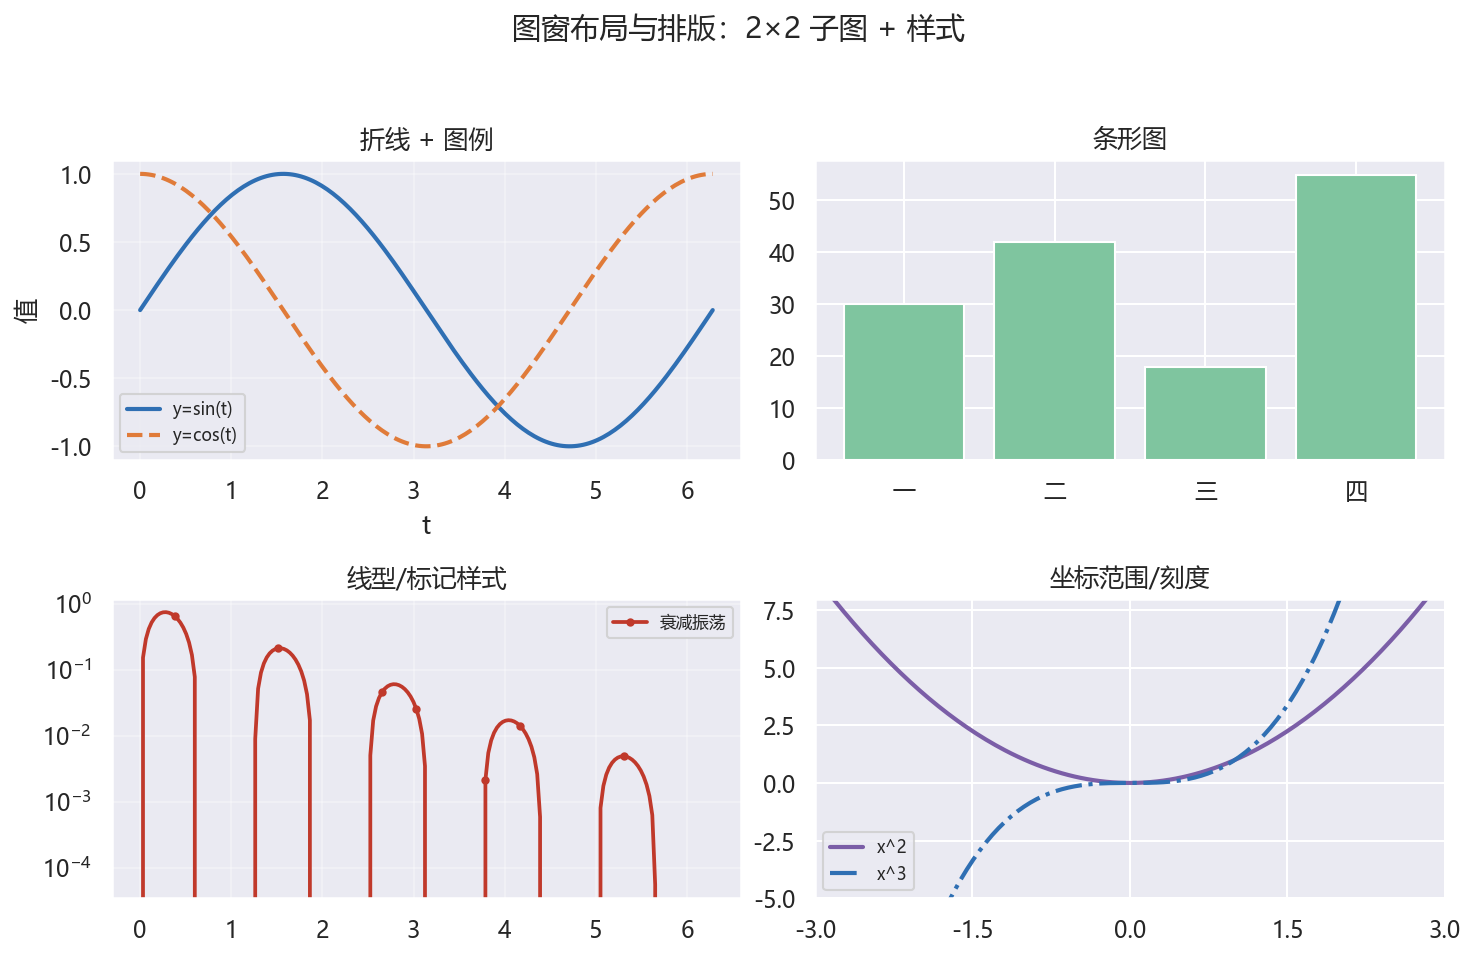
\includegraphics[keepaspectratio,alt={图窗布局示例}]{figures/05-matplotlib/subplots_layout.png}}
\caption{图窗布局示例}
\end{figure}

\subsection{\texorpdfstring{2.8
保存图像：\texttt{savefig}}{2.8 保存图像：savefig}}\label{ux4fddux5b58ux56feux50cfsavefig}

\begin{Shaded}
\begin{Highlighting}[]
\ImportTok{import}\NormalTok{ matplotlib.pyplot }\ImportTok{as}\NormalTok{ plt}
\ImportTok{import}\NormalTok{ os}

\NormalTok{plt.figure(figsize}\OperatorTok{=}\NormalTok{(}\DecValTok{8}\NormalTok{, }\DecValTok{6}\NormalTok{), dpi}\OperatorTok{=}\DecValTok{100}\NormalTok{)}
\NormalTok{plt.plot([}\DecValTok{1}\NormalTok{, }\DecValTok{2}\NormalTok{, }\DecValTok{3}\NormalTok{], [}\DecValTok{4}\NormalTok{, }\DecValTok{3}\NormalTok{, }\DecValTok{2}\NormalTok{])}
\NormalTok{plt.savefig(}\StringTok{\textquotesingle{}my\_plot.png\textquotesingle{}}\NormalTok{, dpi}\OperatorTok{=}\DecValTok{150}\NormalTok{)}
\BuiltInTok{print}\NormalTok{(}\StringTok{\textquotesingle{}exists:\textquotesingle{}}\NormalTok{, os.path.exists(}\StringTok{\textquotesingle{}my\_plot.png\textquotesingle{}}\NormalTok{))}
\end{Highlighting}
\end{Shaded}

\begin{Shaded}
\begin{Highlighting}[]
\NormalTok{exists: True}
\end{Highlighting}
\end{Shaded}

\begin{quote}
\texttt{savefig} 的 \texttt{dpi} 可单独覆盖图窗
DPI；格式由扩展名决定（\texttt{png} / \texttt{jpg} / \texttt{pdf} /
\texttt{svg} 等）。
\end{quote}

\subsection{常见误区}\label{ux5e38ux89c1ux8befux533a-14}

\begin{enumerate}
\def\labelenumi{\arabic{enumi}.}
\tightlist
\item
  \textbf{混用 \texttt{plt} 与 \texttt{ax} 接口}：在面向对象代码中继续用
  \texttt{plt.title}
  可能作用于``当前''轴，子图多了易错。建议一个图中要么纯函数式、要么纯面向对象。
\item
  \textbf{忘记 \texttt{tight\_layout}}：子图标题、轴标签互相重叠。
\item
  \textbf{\texttt{set\_xticks} 与 \texttt{set\_xticklabels}
  混用}：前者设刻度位置，后者改刻度文字。
\item
  \textbf{把 \texttt{figsize} 单位当像素}：实际单位是英寸，配合
  \texttt{dpi} 才得到像素。
\item
  \textbf{\texttt{rcParams} 在 \texttt{seaborn.set\_theme}
  之后设置}：否则字体被覆盖回 Arial（见第 3 节）。
\end{enumerate}

\subsection{思考题}\label{ux601dux8003ux9898-14}

\begin{enumerate}
\def\labelenumi{\arabic{enumi}.}
\tightlist
\item
  \texttt{fig,\ axs\ =\ plt.subplots(3,\ 4)} 中 \texttt{axs.shape}
  是多少？如何访问第 2 行第 3 列子图？
\item
  为什么 \texttt{plt.show()}
  不能在无窗口服务器上显示图形？此时用哪种方法输出？
\item
  \texttt{tight\_layout} 和 \texttt{subplots\_adjust}
  的区别是什么？各自适合什么场景？
\item
  要在每个子图上画不同内容并共用同一 \texttt{x} 轴，\texttt{axs.flat}
  与显式下标哪种更清晰？
\end{enumerate}

\subsection{动手练习（详见
lab）}\label{ux52a8ux624bux7ec3ux4e60ux8be6ux89c1-lab-9}

\begin{itemize}
\tightlist
\item
  创建 2×3 子图，分别画 sin、cos、tan、exp、log、x\^{}2；
\item
  用 \texttt{rcParams} 设置全局字号 12，并为每个子图加中文标题；
\item
  上一题做完后调用 \texttt{fig.tight\_layout()} 观察差异；
\item
  用 \texttt{savefig} 导出 300 DPI 的 PDF。
\end{itemize}

\subsection{延伸阅读}\label{ux5ef6ux4f38ux9605ux8bfb-22}

\begin{itemize}
\tightlist
\item
  Matplotlib 官方``Pyplot
  教程''：https://matplotlib.org/stable/tutorials/pyplot.html
\item
  Matplotlib 官方``面向对象
  API''：https://matplotlib.org/stable/tutorials/introductory/usage.html\#the-object-oriented-interface
\item
  Matplotlib
  官方``文本/字体''：https://matplotlib.org/stable/users/explain/text/text\_props.html
\end{itemize}

\section{03 Seaborn
美化：主题、统计图与分面}\label{seaborn-ux7f8eux5316ux4e3bux9898ux7edfux8ba1ux56feux4e0eux5206ux9762}

\begin{quote}
本节对应原版 5.3 的内容，并增补学习目标、常见误区、思考题与延伸阅读。
配套图：\texttt{figures/05-matplotlib/seaborn\_style.png}（由
\texttt{build/make\_chap5\_figures.py} 生成）。
\end{quote}

\subsection{本节目标}\label{ux672cux8282ux76eeux6807-15}

\begin{itemize}
\tightlist
\item
  理解 Seaborn 与 Matplotlib 的关系；
\item
  会用 \texttt{set\_theme} / \texttt{set\_style} 切换全局主题；
\item
  会用
  \texttt{histplot}、\texttt{kdeplot}、\texttt{boxplot}、\texttt{violinplot}、\texttt{heatmap}
  做统计可视化；
\item
  会用 \texttt{FacetGrid} / \texttt{pairplot} 做分面与成对图；
\item
  会与 Matplotlib 的 \texttt{subplots} 结合做多子图报告图。
\end{itemize}

\subsection{先修}\label{ux5148ux4fee-15}

\begin{itemize}
\tightlist
\item
  第 1--2 节的内容；Pandas DataFrame（\texttt{load\_dataset} 返回的就是
  DataFrame）。
\end{itemize}

\subsection{官方文档/参考入口}\label{ux5b98ux65b9ux6587ux6863ux53c2ux8003ux5165ux53e3-4}

\begin{itemize}
\tightlist
\item
  Seaborn 官方教程：https://seaborn.pydata.org/tutorial.html
\item
  Seaborn 官方 API：https://seaborn.pydata.org/api.html
\item
  Matplotlib
  官方图型画廊：https://matplotlib.org/stable/gallery/index.html
\end{itemize}

\begin{center}\rule{0.5\linewidth}{0.5pt}\end{center}

\subsection{3.1 Seaborn 是什么}\label{seaborn-ux662fux4ec0ux4e48}

Seaborn 建立在 Matplotlib 之上，提供：更口语化的函数名、可直接接受
DataFrame 列名、内置统计（如 KDE、分组箱线）、以及一套美观默认主题。

\textbf{注意}：\texttt{sns.set\_theme(style="darkgrid")} 会重置
Matplotlib 的
\texttt{rcParams}（包括字体），所以\textbf{设置主题后要重新设中文字体}，否则中文标题会变方块。

\begin{Shaded}
\begin{Highlighting}[]
\ImportTok{import}\NormalTok{ seaborn }\ImportTok{as}\NormalTok{ sns}
\ImportTok{import}\NormalTok{ matplotlib }\ImportTok{as}\NormalTok{ mpl}
\ImportTok{import}\NormalTok{ matplotlib.pyplot }\ImportTok{as}\NormalTok{ plt}

\NormalTok{sns.set\_theme(style}\OperatorTok{=}\StringTok{"darkgrid"}\NormalTok{)}
\NormalTok{mpl.rcParams[}\StringTok{"font.sans{-}serif"}\NormalTok{] }\OperatorTok{=}\NormalTok{ [}\StringTok{"Microsoft YaHei"}\NormalTok{, }\StringTok{"SimHei"}\NormalTok{, }\StringTok{"DejaVu Sans"}\NormalTok{]}
\NormalTok{mpl.rcParams[}\StringTok{"axes.unicode\_minus"}\NormalTok{] }\OperatorTok{=} \VariableTok{False}

\NormalTok{tips }\OperatorTok{=}\NormalTok{ sns.load\_dataset(}\StringTok{"tips"}\NormalTok{)}
\BuiltInTok{print}\NormalTok{(}\StringTok{"tips shape:"}\NormalTok{, tips.shape)}
\BuiltInTok{print}\NormalTok{(tips.head(}\DecValTok{3}\NormalTok{).to\_string(index}\OperatorTok{=}\VariableTok{False}\NormalTok{))}
\end{Highlighting}
\end{Shaded}

\begin{Shaded}
\begin{Highlighting}[]
\NormalTok{tips shape: (244, 7)}
\NormalTok{ total\_bill  tip    sex smoker day   time  size}
\NormalTok{      16.99 1.01 Female     No Sun Dinner     2}
\NormalTok{      10.34 1.66   Male     No Sun Dinner     3}
\NormalTok{      21.01 3.50   Male     No Sun Dinner     3}
\end{Highlighting}
\end{Shaded}

\begin{quote}
常见主题：\texttt{darkgrid}（默认）、\texttt{whitegrid}、\texttt{dark}、\texttt{white}、\texttt{ticks}。
\end{quote}

\subsection{3.2 在子图中使用
Seaborn}\label{ux5728ux5b50ux56feux4e2dux4f7fux7528-seaborn}

\begin{Shaded}
\begin{Highlighting}[]
\ImportTok{import}\NormalTok{ seaborn }\ImportTok{as}\NormalTok{ sns}
\ImportTok{import}\NormalTok{ matplotlib.pyplot }\ImportTok{as}\NormalTok{ plt}

\NormalTok{tips }\OperatorTok{=}\NormalTok{ sns.load\_dataset(}\StringTok{"tips"}\NormalTok{)}
\NormalTok{fig, axes }\OperatorTok{=}\NormalTok{ plt.subplots(}\DecValTok{2}\NormalTok{, }\DecValTok{2}\NormalTok{, figsize}\OperatorTok{=}\NormalTok{(}\DecValTok{10}\NormalTok{, }\DecValTok{8}\NormalTok{))}
\NormalTok{sns.lineplot(x}\OperatorTok{=}\StringTok{"tip"}\NormalTok{, y}\OperatorTok{=}\StringTok{"total\_bill"}\NormalTok{, data}\OperatorTok{=}\NormalTok{tips, ax}\OperatorTok{=}\NormalTok{axes[}\DecValTok{0}\NormalTok{, }\DecValTok{0}\NormalTok{])}
\NormalTok{sns.barplot(x}\OperatorTok{=}\StringTok{"sex"}\NormalTok{, y}\OperatorTok{=}\StringTok{"total\_bill"}\NormalTok{, data}\OperatorTok{=}\NormalTok{tips, ax}\OperatorTok{=}\NormalTok{axes[}\DecValTok{0}\NormalTok{, }\DecValTok{1}\NormalTok{])}
\NormalTok{sns.scatterplot(x}\OperatorTok{=}\StringTok{"total\_bill"}\NormalTok{, y}\OperatorTok{=}\StringTok{"tip"}\NormalTok{, hue}\OperatorTok{=}\StringTok{"sex"}\NormalTok{, data}\OperatorTok{=}\NormalTok{tips, ax}\OperatorTok{=}\NormalTok{axes[}\DecValTok{1}\NormalTok{, }\DecValTok{0}\NormalTok{])}
\NormalTok{sns.histplot(data}\OperatorTok{=}\NormalTok{tips[}\StringTok{"total\_bill"}\NormalTok{], ax}\OperatorTok{=}\NormalTok{axes[}\DecValTok{1}\NormalTok{, }\DecValTok{1}\NormalTok{])}
\NormalTok{plt.tight\_layout()}
\BuiltInTok{print}\NormalTok{(}\StringTok{"subplots ok:"}\NormalTok{, axes.shape)}
\end{Highlighting}
\end{Shaded}

\begin{Shaded}
\begin{Highlighting}[]
\NormalTok{subplots ok: (2, 2)}
\end{Highlighting}
\end{Shaded}

\begin{quote}
把 \texttt{data=} 传入 DataFrame，并给
\texttt{x}/\texttt{y}/\texttt{hue} 传列名，Seaborn 自动分组。
\end{quote}

\subsection{3.3 常用统计图}\label{ux5e38ux7528ux7edfux8ba1ux56fe}

\subsubsection{3.3.1 频率直方图 +
核密度线}\label{ux9891ux7387ux76f4ux65b9ux56fe-ux6838ux5bc6ux5ea6ux7ebf}

\begin{Shaded}
\begin{Highlighting}[]
\ImportTok{import}\NormalTok{ seaborn }\ImportTok{as}\NormalTok{ sns}
\ImportTok{import}\NormalTok{ matplotlib.pyplot }\ImportTok{as}\NormalTok{ plt}

\NormalTok{tips }\OperatorTok{=}\NormalTok{ sns.load\_dataset(}\StringTok{"tips"}\NormalTok{)}
\NormalTok{sns.histplot(tips, x}\OperatorTok{=}\StringTok{"total\_bill"}\NormalTok{, kde}\OperatorTok{=}\VariableTok{True}\NormalTok{)}
\NormalTok{plt.show()}
\end{Highlighting}
\end{Shaded}

\subsubsection{3.3.2
概率密度曲线}\label{ux6982ux7387ux5bc6ux5ea6ux66f2ux7ebf}

\begin{Shaded}
\begin{Highlighting}[]
\NormalTok{sns.kdeplot(tips[}\StringTok{"total\_bill"}\NormalTok{], fill}\OperatorTok{=}\VariableTok{True}\NormalTok{)}
\NormalTok{plt.show()}
\end{Highlighting}
\end{Shaded}

\begin{quote}
新版 seaborn 用 \texttt{fill=True}（旧版 \texttt{shade=True} 已弃用）。
\end{quote}

\subsubsection{3.3.3
箱线图与提琴图}\label{ux7bb1ux7ebfux56feux4e0eux63d0ux7434ux56fe}

\begin{Shaded}
\begin{Highlighting}[]
\ImportTok{import}\NormalTok{ seaborn }\ImportTok{as}\NormalTok{ sns}
\ImportTok{import}\NormalTok{ matplotlib.pyplot }\ImportTok{as}\NormalTok{ plt}

\NormalTok{tips }\OperatorTok{=}\NormalTok{ sns.load\_dataset(}\StringTok{"tips"}\NormalTok{)}
\NormalTok{fig, axes }\OperatorTok{=}\NormalTok{ plt.subplots(}\DecValTok{1}\NormalTok{, }\DecValTok{2}\NormalTok{, figsize}\OperatorTok{=}\NormalTok{(}\DecValTok{9}\NormalTok{, }\FloatTok{3.5}\NormalTok{))}
\NormalTok{sns.boxplot(x}\OperatorTok{=}\StringTok{"day"}\NormalTok{, y}\OperatorTok{=}\StringTok{"total\_bill"}\NormalTok{, data}\OperatorTok{=}\NormalTok{tips, ax}\OperatorTok{=}\NormalTok{axes[}\DecValTok{0}\NormalTok{])}
\NormalTok{sns.violinplot(x}\OperatorTok{=}\StringTok{"day"}\NormalTok{, y}\OperatorTok{=}\StringTok{"total\_bill"}\NormalTok{, data}\OperatorTok{=}\NormalTok{tips, ax}\OperatorTok{=}\NormalTok{axes[}\DecValTok{1}\NormalTok{])}
\BuiltInTok{print}\NormalTok{(}\StringTok{"boxes:"}\NormalTok{, }\BuiltInTok{len}\NormalTok{(axes[}\DecValTok{0}\NormalTok{].containers), }\StringTok{"violins:"}\NormalTok{, }\BuiltInTok{len}\NormalTok{(axes[}\DecValTok{1}\NormalTok{].collections))}
\end{Highlighting}
\end{Shaded}

\begin{Shaded}
\begin{Highlighting}[]
\NormalTok{boxes: 1  violins: 4}
\end{Highlighting}
\end{Shaded}

\subsubsection{3.3.4 热力图}\label{ux70edux529bux56fe}

\begin{Shaded}
\begin{Highlighting}[]
\ImportTok{import}\NormalTok{ seaborn }\ImportTok{as}\NormalTok{ sns}
\ImportTok{import}\NormalTok{ matplotlib.pyplot }\ImportTok{as}\NormalTok{ plt}

\NormalTok{flights }\OperatorTok{=}\NormalTok{ sns.load\_dataset(}\StringTok{"flights"}\NormalTok{)}
\NormalTok{flights\_pivot }\OperatorTok{=}\NormalTok{ flights.pivot\_table(index}\OperatorTok{=}\StringTok{"month"}\NormalTok{, columns}\OperatorTok{=}\StringTok{"year"}\NormalTok{, values}\OperatorTok{=}\StringTok{"passengers"}\NormalTok{, observed}\OperatorTok{=}\VariableTok{False}\NormalTok{)}
\NormalTok{sns.heatmap(flights\_pivot, annot}\OperatorTok{=}\VariableTok{True}\NormalTok{, fmt}\OperatorTok{=}\StringTok{".0f"}\NormalTok{)}
\BuiltInTok{print}\NormalTok{(}\StringTok{"pivot shape:"}\NormalTok{, flights\_pivot.shape)}
\end{Highlighting}
\end{Shaded}

\begin{Shaded}
\begin{Highlighting}[]
\NormalTok{pivot shape: (12, 12)}
\end{Highlighting}
\end{Shaded}

\subsubsection{3.3.5 成对关系图}\label{ux6210ux5bf9ux5173ux7cfbux56fe}

\begin{Shaded}
\begin{Highlighting}[]
\ImportTok{import}\NormalTok{ seaborn }\ImportTok{as}\NormalTok{ sns}

\NormalTok{tips }\OperatorTok{=}\NormalTok{ sns.load\_dataset(}\StringTok{"tips"}\NormalTok{)}
\NormalTok{g }\OperatorTok{=}\NormalTok{ sns.pairplot(tips, hue}\OperatorTok{=}\StringTok{"day"}\NormalTok{)}
\BuiltInTok{print}\NormalTok{(}\StringTok{"pairplot grid shape:"}\NormalTok{, g.axes.shape)}
\end{Highlighting}
\end{Shaded}

\begin{Shaded}
\begin{Highlighting}[]
\NormalTok{pairplot grid shape: (3, 3)}
\end{Highlighting}
\end{Shaded}

\subsection{\texorpdfstring{3.4 分面与多图：\texttt{FacetGrid} /
\texttt{PairGrid}}{3.4 分面与多图：FacetGrid / PairGrid}}\label{ux5206ux9762ux4e0eux591aux56fefacetgrid-pairgrid}

\begin{Shaded}
\begin{Highlighting}[]
\ImportTok{import}\NormalTok{ seaborn }\ImportTok{as}\NormalTok{ sns}
\ImportTok{import}\NormalTok{ matplotlib.pyplot }\ImportTok{as}\NormalTok{ plt}

\NormalTok{tips }\OperatorTok{=}\NormalTok{ sns.load\_dataset(}\StringTok{"tips"}\NormalTok{)}
\NormalTok{g }\OperatorTok{=}\NormalTok{ sns.FacetGrid(tips, col}\OperatorTok{=}\StringTok{"day"}\NormalTok{, col\_wrap}\OperatorTok{=}\DecValTok{4}\NormalTok{)}
\NormalTok{g.}\BuiltInTok{map}\NormalTok{(sns.lineplot, }\StringTok{"total\_bill"}\NormalTok{, }\StringTok{"tip"}\NormalTok{)}
\NormalTok{g.add\_legend()}
\BuiltInTok{print}\NormalTok{(}\StringTok{"FacetGrid axes:"}\NormalTok{, }\BuiltInTok{len}\NormalTok{(g.axes.flat))}
\end{Highlighting}
\end{Shaded}

\begin{Shaded}
\begin{Highlighting}[]
\NormalTok{FacetGrid axes: 4}
\end{Highlighting}
\end{Shaded}

\begin{quote}
\texttt{FacetGrid} 按列取值把数据切成多个子图；\texttt{col\_wrap}
控制每行放几个。\texttt{PairGrid} 则用于变量两两成对。
\end{quote}

\begin{figure}
\centering
\pandocbounded{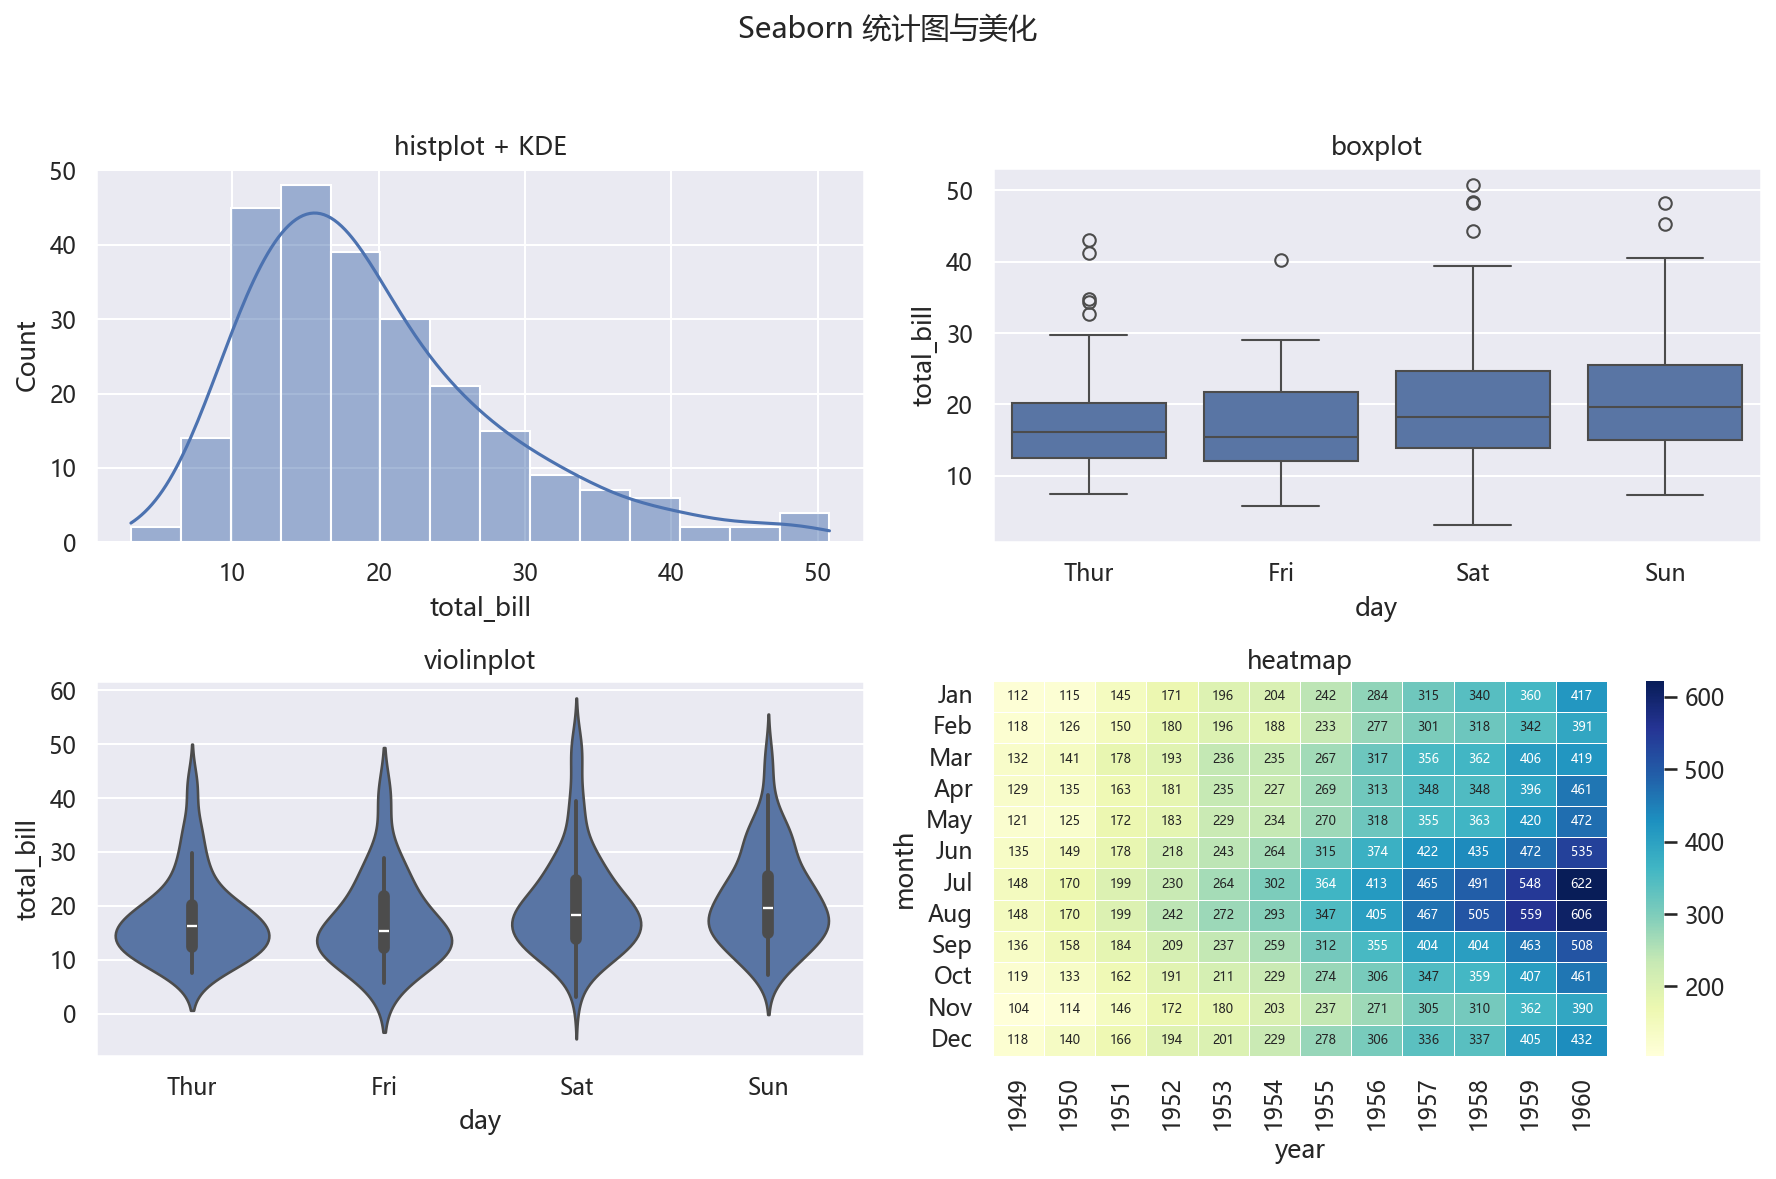
\includegraphics[keepaspectratio,alt={Seaborn 统计图与美化}]{figures/05-matplotlib/seaborn_style.png}}
\caption{Seaborn 统计图与美化}
\end{figure}

\subsection{常见误区}\label{ux5e38ux89c1ux8befux533a-15}

\begin{enumerate}
\def\labelenumi{\arabic{enumi}.}
\tightlist
\item
  \textbf{\texttt{set\_theme} 之后不重设中文字体}：中文标题变方块。
\item
  \textbf{把旧版 \texttt{shade=True} 当新 API}：新版本改为
  \texttt{fill=True}，旧参数已弃用。
\item
  \textbf{\texttt{sns.boxplot} 返回的 \texttt{ax} 与 Matplotlib 子图混用
  \texttt{plt.title}}：多个子图时易错。
\item
  \textbf{\texttt{load\_dataset} 依赖网络}：若要离线教学，可先用
  \texttt{pd.DataFrame(...)} 构造样例数据。
\item
  \textbf{给 \texttt{heatmap} 的 \texttt{fmt="d"} 传浮点数据}：应改用
  \texttt{fmt=".0f"} 或 \texttt{.2f}。
\end{enumerate}

\subsection{思考题}\label{ux601dux8003ux9898-15}

\begin{enumerate}
\def\labelenumi{\arabic{enumi}.}
\tightlist
\item
  \texttt{sns.set\_theme} 与 \texttt{plt.style.use} 有何异同？
\item
  \texttt{boxplot} 与 \texttt{violinplot} 分别适合什么场景？
\item
  为什么 \texttt{FacetGrid} 比手动 \texttt{subplots}
  循环更适合``按类别分面''？
\item
  在 Seaborn 图中能否继续用 Matplotlib 的
  \texttt{set\_xticks}？如何操作？
\end{enumerate}

\subsection{动手练习（详见
lab）}\label{ux52a8ux624bux7ec3ux4e60ux8be6ux89c1-lab-10}

\begin{itemize}
\tightlist
\item
  用 \texttt{tips} 画 \texttt{day} 分组的箱线图，并切换
  \texttt{whitegrid} / \texttt{ticks} 主题对比；
\item
  用 \texttt{flights} 透视表画热力图，并自定义 \texttt{cmap}；
\item
  用 \texttt{penguins} 数据集做一对 \texttt{pairplot}；
\item
  用 \texttt{FacetGrid} 按 \texttt{sex} 分面画 \texttt{total\_bill}
  的直方图。
\end{itemize}

\subsection{延伸阅读}\label{ux5ef6ux4f38ux9605ux8bfb-23}

\begin{itemize}
\tightlist
\item
  Seaborn 官方教程：https://seaborn.pydata.org/tutorial.html
\item
  Seaborn 官方 API：https://seaborn.pydata.org/api.html
\item
  Matplotlib + Seaborn
  结合示例：https://seaborn.pydata.org/examples/index.html
\end{itemize}

\section{04
综合案例：传感器信号分析与分组报告图}\label{ux7efcux5408ux6848ux4f8bux4f20ux611fux5668ux4fe1ux53f7ux5206ux6790ux4e0eux5206ux7ec4ux62a5ux544aux56fe}

\begin{quote}
本章新增综合案例，用于把 01--03 的知识串起来：\textbf{基础图表 +
多子图/排版 + Seaborn 统计图}。 所有代码均可在 matplotlib ≥ 3.8、seaborn
≥ 0.13 环境运行；配图由 \texttt{build/make\_chap5\_figures.py} 生成。
\end{quote}

\subsection{案例背景}\label{ux6848ux4f8bux80ccux666f-2}

假设你拿到一段``传感器信号''采样（含噪声）与一批分组测量值，需要输出一张\textbf{数据分析报告图}：

\begin{enumerate}
\def\labelenumi{\arabic{enumi}.}
\tightlist
\item
  左上：时间序列折线图，把原始信号与滑动平均后的平滑信号叠在一起；
\item
  右上：信号幅值直方图 + 核密度估计（Seaborn）；
\item
  左下：对照组 / 实验组的分组散点图；
\item
  右下：几个变量之间的相关矩阵热力图。
\end{enumerate}

这正是第 1 章的``数据能画出来'' + 第 2 章的``多子图排版'' + 第 3
章``Seaborn 统计图''的联合应用。

\subsection{步骤
1：生成合成信号并平滑}\label{ux6b65ux9aa4-1ux751fux6210ux5408ux6210ux4fe1ux53f7ux5e76ux5e73ux6ed1}

\begin{Shaded}
\begin{Highlighting}[]
\ImportTok{import}\NormalTok{ numpy }\ImportTok{as}\NormalTok{ np}
\ImportTok{import}\NormalTok{ pandas }\ImportTok{as}\NormalTok{ pd}
\ImportTok{import}\NormalTok{ matplotlib.pyplot }\ImportTok{as}\NormalTok{ plt}
\ImportTok{import}\NormalTok{ seaborn }\ImportTok{as}\NormalTok{ sns}

\NormalTok{rng }\OperatorTok{=}\NormalTok{ np.random.default\_rng(}\DecValTok{2025}\NormalTok{)   }\CommentTok{\# 固定种子，保证可复现}
\NormalTok{n }\OperatorTok{=} \DecValTok{400}
\NormalTok{t }\OperatorTok{=}\NormalTok{ np.linspace(}\DecValTok{0}\NormalTok{, }\DecValTok{20}\NormalTok{, n)}
\NormalTok{signal }\OperatorTok{=} \DecValTok{3} \OperatorTok{*}\NormalTok{ np.sin(}\DecValTok{2} \OperatorTok{*}\NormalTok{ np.pi }\OperatorTok{*} \FloatTok{0.25} \OperatorTok{*}\NormalTok{ t) }\OperatorTok{+} \FloatTok{0.6} \OperatorTok{*}\NormalTok{ np.cos(}\DecValTok{2} \OperatorTok{*}\NormalTok{ np.pi }\OperatorTok{*} \FloatTok{1.1} \OperatorTok{*}\NormalTok{ t) }\OperatorTok{+} \FloatTok{0.8}
\NormalTok{y }\OperatorTok{=}\NormalTok{ signal }\OperatorTok{+}\NormalTok{ rng.normal(}\DecValTok{0}\NormalTok{, }\FloatTok{0.5}\NormalTok{, n)}
\NormalTok{smoothed }\OperatorTok{=}\NormalTok{ pd.Series(y).rolling(window}\OperatorTok{=}\DecValTok{15}\NormalTok{, center}\OperatorTok{=}\VariableTok{True}\NormalTok{).mean().to\_numpy()}

\BuiltInTok{print}\NormalTok{(}\StringTok{"信号长度 n ="}\NormalTok{, n)}
\BuiltInTok{print}\NormalTok{(}\StringTok{"原始信号  均值 ="}\NormalTok{, }\BuiltInTok{round}\NormalTok{(}\BuiltInTok{float}\NormalTok{(y.mean()), }\DecValTok{3}\NormalTok{), }\StringTok{" 标准差 ="}\NormalTok{, }\BuiltInTok{round}\NormalTok{(}\BuiltInTok{float}\NormalTok{(y.std()), }\DecValTok{3}\NormalTok{))}
\BuiltInTok{print}\NormalTok{(}\StringTok{"平滑信号  均值 ="}\NormalTok{, }\BuiltInTok{round}\NormalTok{(}\BuiltInTok{float}\NormalTok{(np.nanmean(smoothed)), }\DecValTok{3}\NormalTok{))}
\BuiltInTok{print}\NormalTok{(}\StringTok{"平滑信号 前 5 个 ="}\NormalTok{, np.}\BuiltInTok{round}\NormalTok{(smoothed[:}\DecValTok{5}\NormalTok{], }\DecValTok{3}\NormalTok{))}
\end{Highlighting}
\end{Shaded}

\begin{Shaded}
\begin{Highlighting}[]
\NormalTok{信号长度 n = 400}
\NormalTok{原始信号  均值 = 0.795  标准差 = 2.244}
\NormalTok{平滑信号  均值 = 0.797}
\NormalTok{平滑信号 前 5 个 = [nan nan nan nan nan]}
\end{Highlighting}
\end{Shaded}

\begin{quote}
\texttt{rolling(window=15,\ center=True)}
做中心化滑动平均；两端窗口不满时为 NaN，属正常现象。
\end{quote}

\subsection{步骤
2：生成分组数据与相关矩阵}\label{ux6b65ux9aa4-2ux751fux6210ux5206ux7ec4ux6570ux636eux4e0eux76f8ux5173ux77e9ux9635}

\begin{Shaded}
\begin{Highlighting}[]
\NormalTok{rng2 }\OperatorTok{=}\NormalTok{ np.random.default\_rng(}\DecValTok{1}\NormalTok{)}
\NormalTok{group }\OperatorTok{=}\NormalTok{ rng2.choice([}\StringTok{"对照组"}\NormalTok{, }\StringTok{"实验组"}\NormalTok{], size}\OperatorTok{=}\DecValTok{250}\NormalTok{, p}\OperatorTok{=}\NormalTok{[}\FloatTok{0.5}\NormalTok{, }\FloatTok{0.5}\NormalTok{])}
\NormalTok{val }\OperatorTok{=}\NormalTok{ np.where(group }\OperatorTok{==} \StringTok{"实验组"}\NormalTok{, rng2.normal(}\FloatTok{5.2}\NormalTok{, }\FloatTok{1.1}\NormalTok{, }\DecValTok{250}\NormalTok{), rng2.normal(}\FloatTok{4.0}\NormalTok{, }\FloatTok{1.0}\NormalTok{, }\DecValTok{250}\NormalTok{))}

\NormalTok{df\_corr }\OperatorTok{=}\NormalTok{ pd.DataFrame(\{}
    \StringTok{"x1"}\NormalTok{: rng2.normal(}\DecValTok{0}\NormalTok{, }\DecValTok{1}\NormalTok{, }\DecValTok{300}\NormalTok{),}
    \StringTok{"x2"}\NormalTok{: rng2.normal(}\DecValTok{0}\NormalTok{, }\DecValTok{1}\NormalTok{, }\DecValTok{300}\NormalTok{),}
    \StringTok{"x3"}\NormalTok{: rng2.normal(}\DecValTok{0}\NormalTok{, }\DecValTok{1}\NormalTok{, }\DecValTok{300}\NormalTok{),}
\NormalTok{\})}
\NormalTok{df\_corr[}\StringTok{"x4"}\NormalTok{] }\OperatorTok{=} \FloatTok{0.8} \OperatorTok{*}\NormalTok{ df\_corr[}\StringTok{"x1"}\NormalTok{] }\OperatorTok{+}\NormalTok{ rng2.normal(}\DecValTok{0}\NormalTok{, }\FloatTok{0.6}\NormalTok{, }\DecValTok{300}\NormalTok{)}
\NormalTok{corr }\OperatorTok{=}\NormalTok{ df\_corr.corr()}

\BuiltInTok{print}\NormalTok{(}\StringTok{"对照组均值 ="}\NormalTok{, }\BuiltInTok{round}\NormalTok{(}\BuiltInTok{float}\NormalTok{(val[group }\OperatorTok{==} \StringTok{"对照组"}\NormalTok{].mean()), }\DecValTok{3}\NormalTok{))}
\BuiltInTok{print}\NormalTok{(}\StringTok{"实验组均值 ="}\NormalTok{, }\BuiltInTok{round}\NormalTok{(}\BuiltInTok{float}\NormalTok{(val[group }\OperatorTok{==} \StringTok{"实验组"}\NormalTok{].mean()), }\DecValTok{3}\NormalTok{))}
\BuiltInTok{print}\NormalTok{(}\StringTok{"相关系数 x1{-}x4 ="}\NormalTok{, }\BuiltInTok{round}\NormalTok{(}\BuiltInTok{float}\NormalTok{(corr.loc[}\StringTok{"x1"}\NormalTok{, }\StringTok{"x4"}\NormalTok{]), }\DecValTok{3}\NormalTok{))}
\BuiltInTok{print}\NormalTok{(}\StringTok{"相关系数 x1{-}x2 ="}\NormalTok{, }\BuiltInTok{round}\NormalTok{(}\BuiltInTok{float}\NormalTok{(corr.loc[}\StringTok{"x1"}\NormalTok{, }\StringTok{"x2"}\NormalTok{]), }\DecValTok{3}\NormalTok{))}
\BuiltInTok{print}\NormalTok{()}
\BuiltInTok{print}\NormalTok{(corr.}\BuiltInTok{round}\NormalTok{(}\DecValTok{2}\NormalTok{).to\_string())}
\end{Highlighting}
\end{Shaded}

\begin{Shaded}
\begin{Highlighting}[]
\NormalTok{对照组均值 = 3.874}
\NormalTok{实验组均值 = 5.274}
\NormalTok{相关系数 x1{-}x4 = 0.819}
\NormalTok{相关系数 x1{-}x2 = {-}0.097}

\NormalTok{      x1    x2    x3    x4}
\NormalTok{x1  1.00 {-}0.10  0.06  0.82}
\NormalTok{x2 {-}0.10  1.00 {-}0.05 {-}0.07}
\NormalTok{x3  0.06 {-}0.05  1.00  0.07}
\NormalTok{x4  0.82 {-}0.07  0.07  1.00}
\end{Highlighting}
\end{Shaded}

\begin{quote}
因为构造时 \texttt{x4} 由 \texttt{x1} 主导，所以 \texttt{x1–x4}
相关系数约 0.8，热力图一眼可辨。
\end{quote}

\subsection{步骤 3：绘制 2×2
报告图}\label{ux6b65ux9aa4-3ux7ed8ux5236-22-ux62a5ux544aux56fe}

\begin{quote}
本步依赖步骤 1/2 中定义的
\texttt{t}、\texttt{y}、\texttt{smoothed}、\texttt{group}、\texttt{val}、\texttt{corr}，请按顺序运行。
\end{quote}

\begin{Shaded}
\begin{Highlighting}[]
\CommentTok{\#\# 中文字体（注意：set\_theme 会覆盖，这里放在绘图前重新设置）}
\ImportTok{import}\NormalTok{ matplotlib }\ImportTok{as}\NormalTok{ mpl}
\NormalTok{mpl.rcParams[}\StringTok{"font.sans{-}serif"}\NormalTok{] }\OperatorTok{=}\NormalTok{ [}\StringTok{"Microsoft YaHei"}\NormalTok{, }\StringTok{"SimHei"}\NormalTok{, }\StringTok{"DejaVu Sans"}\NormalTok{]}
\NormalTok{mpl.rcParams[}\StringTok{"axes.unicode\_minus"}\NormalTok{] }\OperatorTok{=} \VariableTok{False}

\NormalTok{fig, axes }\OperatorTok{=}\NormalTok{ plt.subplots(}\DecValTok{2}\NormalTok{, }\DecValTok{2}\NormalTok{, figsize}\OperatorTok{=}\NormalTok{(}\DecValTok{12}\NormalTok{, }\FloatTok{8.5}\NormalTok{))}
\NormalTok{fig.suptitle(}\StringTok{"综合案例：传感器信号观测与分组分析"}\NormalTok{, fontsize}\OperatorTok{=}\DecValTok{15}\NormalTok{)}

\NormalTok{axes[}\DecValTok{0}\NormalTok{, }\DecValTok{0}\NormalTok{].plot(t, y, color}\OperatorTok{=}\StringTok{"\#c8d8e8"}\NormalTok{, lw}\OperatorTok{=}\DecValTok{1}\NormalTok{, label}\OperatorTok{=}\StringTok{"原始信号"}\NormalTok{)}
\NormalTok{axes[}\DecValTok{0}\NormalTok{, }\DecValTok{0}\NormalTok{].plot(t, smoothed, color}\OperatorTok{=}\StringTok{"\#c0392b"}\NormalTok{, lw}\OperatorTok{=}\FloatTok{2.2}\NormalTok{, label}\OperatorTok{=}\StringTok{"滑动平均(窗口=15)"}\NormalTok{)}
\NormalTok{axes[}\DecValTok{0}\NormalTok{, }\DecValTok{0}\NormalTok{].set\_title(}\StringTok{"时间序列：原始信号 vs 平滑"}\NormalTok{)}
\NormalTok{axes[}\DecValTok{0}\NormalTok{, }\DecValTok{0}\NormalTok{].set\_xlabel(}\StringTok{"时间 t"}\NormalTok{)}\OperatorTok{;}\NormalTok{ axes[}\DecValTok{0}\NormalTok{, }\DecValTok{0}\NormalTok{].set\_ylabel(}\StringTok{"幅值"}\NormalTok{)}
\NormalTok{axes[}\DecValTok{0}\NormalTok{, }\DecValTok{0}\NormalTok{].legend(fontsize}\OperatorTok{=}\DecValTok{8}\NormalTok{)}\OperatorTok{;}\NormalTok{ axes[}\DecValTok{0}\NormalTok{, }\DecValTok{0}\NormalTok{].grid(alpha}\OperatorTok{=}\FloatTok{0.3}\NormalTok{)}

\NormalTok{sns.histplot(x}\OperatorTok{=}\NormalTok{y, kde}\OperatorTok{=}\VariableTok{True}\NormalTok{, color}\OperatorTok{=}\StringTok{"\#2f6fb3"}\NormalTok{, ax}\OperatorTok{=}\NormalTok{axes[}\DecValTok{0}\NormalTok{, }\DecValTok{1}\NormalTok{])}
\NormalTok{axes[}\DecValTok{0}\NormalTok{, }\DecValTok{1}\NormalTok{].set\_title(}\StringTok{"信号幅值分布"}\NormalTok{)}
\NormalTok{axes[}\DecValTok{0}\NormalTok{, }\DecValTok{1}\NormalTok{].set\_xlabel(}\StringTok{"幅值"}\NormalTok{)}

\NormalTok{axes[}\DecValTok{1}\NormalTok{, }\DecValTok{0}\NormalTok{].scatter(group[group }\OperatorTok{==} \StringTok{"对照组"}\NormalTok{], val[group }\OperatorTok{==} \StringTok{"对照组"}\NormalTok{],}
\NormalTok{                   color}\OperatorTok{=}\StringTok{"\#7fc59f"}\NormalTok{, s}\OperatorTok{=}\DecValTok{22}\NormalTok{, alpha}\OperatorTok{=}\FloatTok{0.75}\NormalTok{, label}\OperatorTok{=}\StringTok{"对照组"}\NormalTok{)}
\NormalTok{axes[}\DecValTok{1}\NormalTok{, }\DecValTok{0}\NormalTok{].scatter(group[group }\OperatorTok{==} \StringTok{"实验组"}\NormalTok{], val[group }\OperatorTok{==} \StringTok{"实验组"}\NormalTok{],}
\NormalTok{                   color}\OperatorTok{=}\StringTok{"\#e07b39"}\NormalTok{, s}\OperatorTok{=}\DecValTok{22}\NormalTok{, alpha}\OperatorTok{=}\FloatTok{0.75}\NormalTok{, label}\OperatorTok{=}\StringTok{"实验组"}\NormalTok{)}
\NormalTok{axes[}\DecValTok{1}\NormalTok{, }\DecValTok{0}\NormalTok{].set\_title(}\StringTok{"分组散点图"}\NormalTok{)}
\NormalTok{axes[}\DecValTok{1}\NormalTok{, }\DecValTok{0}\NormalTok{].set\_xlabel(}\StringTok{"分组"}\NormalTok{)}\OperatorTok{;}\NormalTok{ axes[}\DecValTok{1}\NormalTok{, }\DecValTok{0}\NormalTok{].set\_ylabel(}\StringTok{"测量值"}\NormalTok{)}
\NormalTok{axes[}\DecValTok{1}\NormalTok{, }\DecValTok{0}\NormalTok{].legend(fontsize}\OperatorTok{=}\DecValTok{8}\NormalTok{)}\OperatorTok{;}\NormalTok{ axes[}\DecValTok{1}\NormalTok{, }\DecValTok{0}\NormalTok{].grid(alpha}\OperatorTok{=}\FloatTok{0.3}\NormalTok{)}

\NormalTok{sns.heatmap(corr, annot}\OperatorTok{=}\VariableTok{True}\NormalTok{, fmt}\OperatorTok{=}\StringTok{".2f"}\NormalTok{, cmap}\OperatorTok{=}\StringTok{"coolwarm"}\NormalTok{, vmin}\OperatorTok{={-}}\DecValTok{1}\NormalTok{, vmax}\OperatorTok{=}\DecValTok{1}\NormalTok{,}
\NormalTok{            ax}\OperatorTok{=}\NormalTok{axes[}\DecValTok{1}\NormalTok{, }\DecValTok{1}\NormalTok{], annot\_kws}\OperatorTok{=}\NormalTok{\{}\StringTok{"fontsize"}\NormalTok{: }\DecValTok{9}\NormalTok{\})}
\NormalTok{axes[}\DecValTok{1}\NormalTok{, }\DecValTok{1}\NormalTok{].set\_title(}\StringTok{"变量间相关矩阵热力图"}\NormalTok{)}

\NormalTok{fig.tight\_layout(rect}\OperatorTok{=}\NormalTok{[}\DecValTok{0}\NormalTok{, }\DecValTok{0}\NormalTok{, }\DecValTok{1}\NormalTok{, }\FloatTok{0.95}\NormalTok{])}
\NormalTok{fig.savefig(}\StringTok{"case\_study.png"}\NormalTok{, dpi}\OperatorTok{=}\DecValTok{150}\NormalTok{)}
\BuiltInTok{print}\NormalTok{(}\StringTok{"已保存 case\_study.png"}\NormalTok{)}
\end{Highlighting}
\end{Shaded}

输出：\texttt{已保存\ case\_study.png}，并得到下图。

\begin{figure}
\centering
\pandocbounded{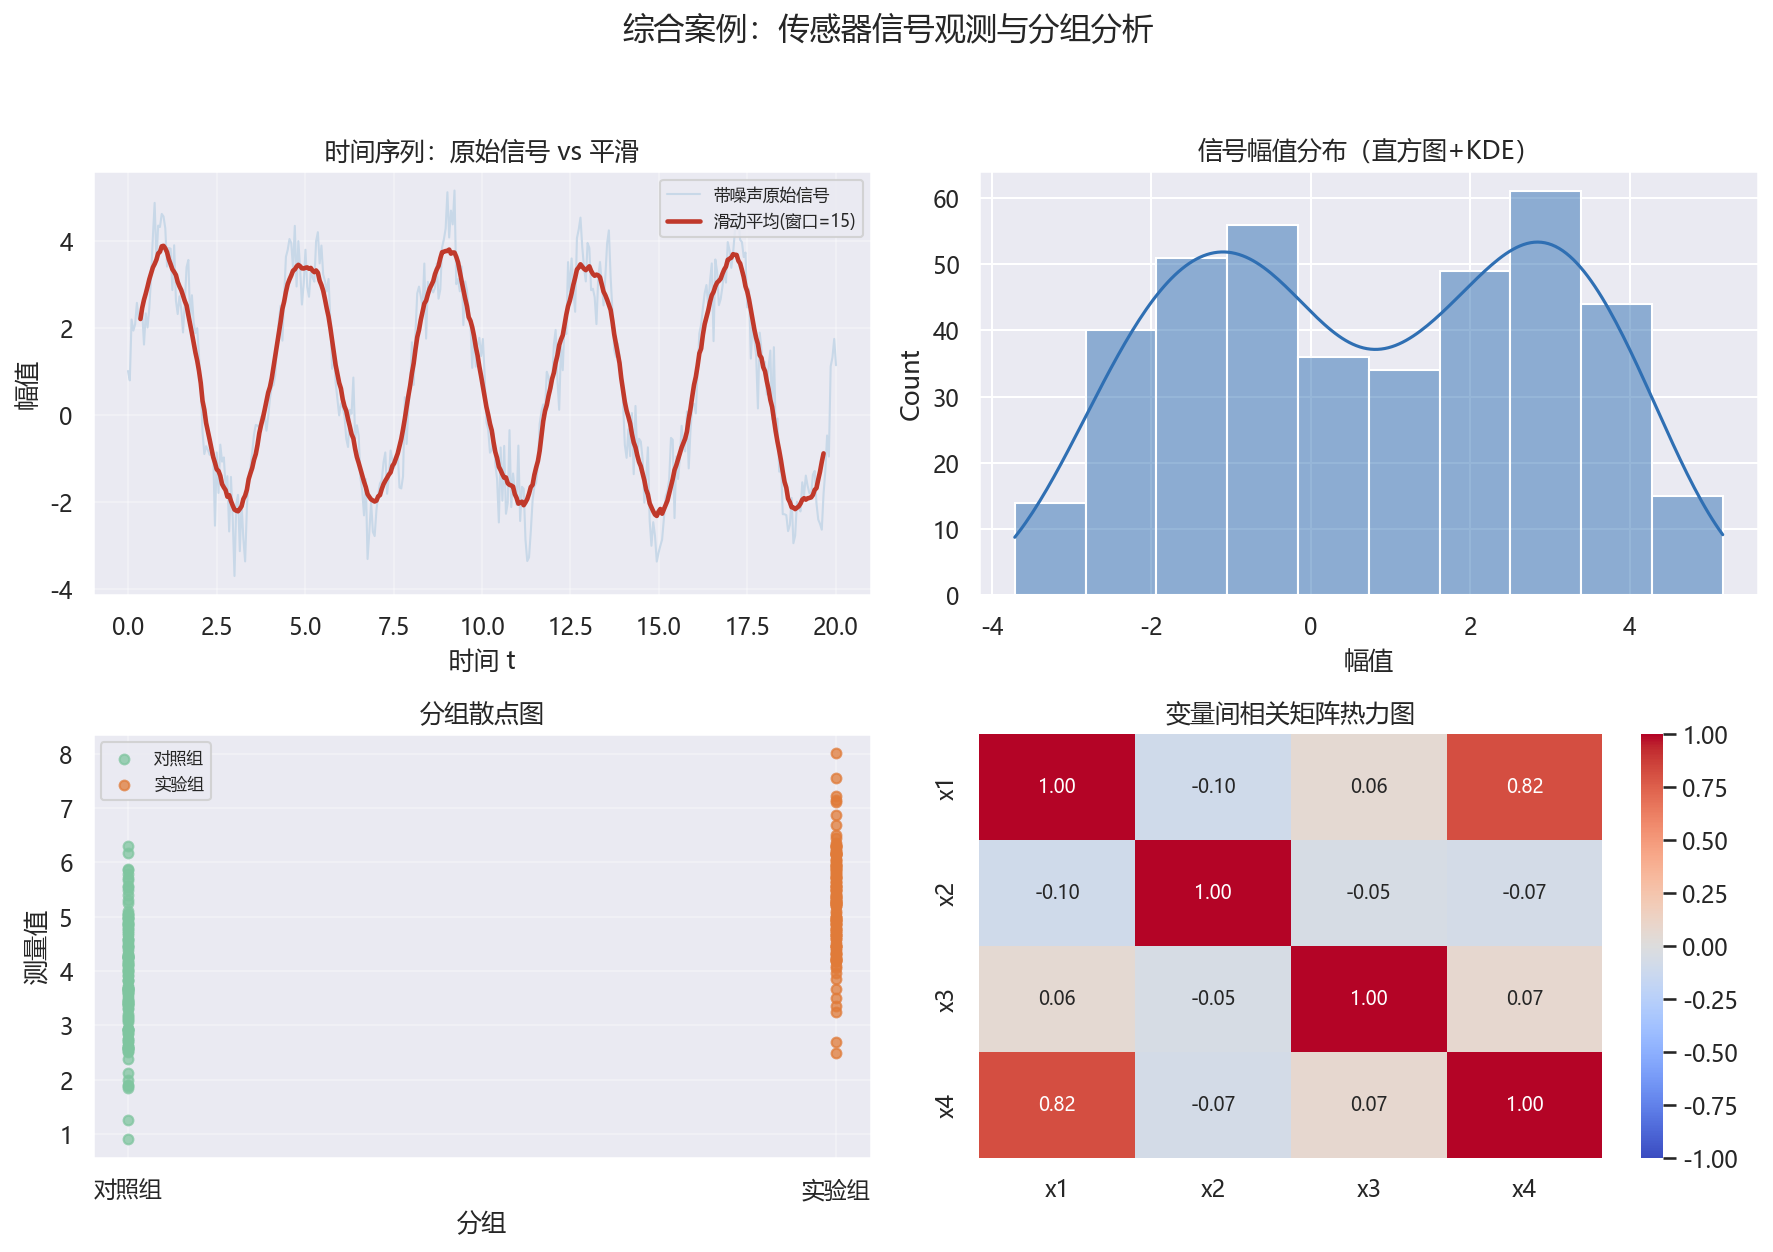
\includegraphics[keepaspectratio,alt={综合案例报告图}]{figures/05-matplotlib/case_study.png}}
\caption{综合案例报告图}
\end{figure}

\subsection{分析与延伸}\label{ux5206ux6790ux4e0eux5ef6ux4f38}

\begin{itemize}
\tightlist
\item
  \textbf{左上}：原始信号噪声明显，滑动平均后波形更平滑------直观体会``平滑窗口''对信噪比的影响；
\item
  \textbf{右上}：信号幅值近似正态分布（叠加噪声的多频正弦叠加），KDE
  与直方图吻合；
\item
  \textbf{左下}：实验组测量值整体高于对照组，散点图可直接看出两组的中心差异；
\item
  \textbf{右下}：\texttt{x1} 与 \texttt{x4} 相关系数约
  0.8，热力图让``共线性''一目了然。
\end{itemize}

\subsubsection{拓展任务}\label{ux62d3ux5c55ux4efbux52a1-7}

\begin{enumerate}
\def\labelenumi{\arabic{enumi}.}
\tightlist
\item
  把平滑窗口从 15 改为 5 / 31，比较左上图平滑程度与失真；
\item
  用 \texttt{sns.kdeplot} 分开画对照/实验两组的密度曲线，观察重叠区域；
\item
  把相关矩阵改用 \texttt{sns.clustermap} 展示变量聚类；
\item
  将报告图导出为 PDF，并比较不同 \texttt{dpi} 的文件大小。
\end{enumerate}

\subsection{延伸阅读}\label{ux5ef6ux4f38ux9605ux8bfb-24}

\begin{itemize}
\tightlist
\item
  Matplotlib
  多子图：https://matplotlib.org/stable/tutorials/intermediate/subplots.html
\item
  Seaborn
  分布图：https://seaborn.pydata.org/generated/seaborn.histplot.html
\item
  Pandas
  \texttt{rolling}：https://pandas.pydata.org/docs/reference/api/pandas.DataFrame.rolling.html
\end{itemize}

\section{05
常见误区与技巧}\label{ux5e38ux89c1ux8befux533aux4e0eux6280ux5de7-4}

\begin{quote}
本章为新增``查漏补缺''页：把学生最容易踩的坑集中列出，并给出正确的写法和性能技巧。
\end{quote}

\subsection{1.
高频误区速查表}\label{ux9ad8ux9891ux8befux533aux901fux67e5ux8868-4}

{\def\LTcaptype{none} % do not increment counter
\begin{longtable}[]{@{}
  >{\raggedright\arraybackslash}p{(\linewidth - 6\tabcolsep) * \real{0.2500}}
  >{\raggedright\arraybackslash}p{(\linewidth - 6\tabcolsep) * \real{0.2500}}
  >{\raggedright\arraybackslash}p{(\linewidth - 6\tabcolsep) * \real{0.2500}}
  >{\raggedright\arraybackslash}p{(\linewidth - 6\tabcolsep) * \real{0.2500}}@{}}
\toprule\noalign{}
\begin{minipage}[b]{\linewidth}\raggedright
\#
\end{minipage} & \begin{minipage}[b]{\linewidth}\raggedright
误区 / 错误写法
\end{minipage} & \begin{minipage}[b]{\linewidth}\raggedright
正确做法
\end{minipage} & \begin{minipage}[b]{\linewidth}\raggedright
原因
\end{minipage} \\
\midrule\noalign{}
\endhead
\bottomrule\noalign{}
\endlastfoot
1 & 只 \texttt{plt.plot} 不 \texttt{plt.show()}/\texttt{savefig} &
脚本中用 \texttt{plt.savefig}；交互环境用 \texttt{plt.show()} &
图可能``画了不显示/不保存'' \\
2 & 面向对象代码里混用 \texttt{plt.title} & 用
\texttt{ax.set\_title(...)} & 多子图时 \texttt{plt}
作用于当前轴，易错 \\
3 & 忘记 \texttt{ax.set\_xticks} 与 \texttt{set\_xticklabels} 的区别 &
前者设位置，后者改文字 & 两个函数语义不同 \\
4 & 误以为 \texttt{figsize} 是像素 & 单位是英寸，需乘 \texttt{dpi}
得到像素 & 单位语义错误 \\
5 & \texttt{rcParams} 在 seaborn \texttt{set\_theme} 之前设置 &
主题之后重新设置字体 & \texttt{set\_theme} 会重置
\texttt{font.sans-serif} \\
6 & 对 \texttt{heatmap} 传 \texttt{fmt="d"} 而数据是浮点 & 改用
\texttt{fmt=".0f"} 或 \texttt{.2f} & 格式码与数据类型不匹配 \\
7 & 用旧版 \texttt{shade=True} & 用 \texttt{fill=True} &
新版参数已改名 \\
8 & \texttt{plt.subplots(2,2)} 后用 \texttt{plt.subplot()} 再画 &
统一用返回的 \texttt{axs.flat} & 两个接口混用会叠加到错误的轴 \\
9 & 忘记 \texttt{np.meshgrid} 就画 3D 曲面 & 先 \texttt{np.meshgrid}
生成 2D 网格 & 曲面需要网格化的 X, Y, Z \\
10 & 误以为一张图只能有一个 Figure & 一个脚本可多 Figure；用
\texttt{plt.figure()} 新建 & 状态管理理解偏差 \\
11 & 中文标题变方块还不设字体 & 设
\texttt{rcParams{[}"font.sans-serif"{]}\ =\ {[}"Microsoft\ YaHei",\ ...{]}}
& 默认字体不含中文字形 \\
12 & 频繁 \texttt{plt.show()} 后又想改 \texttt{rcParams} &
先设全局参数再绘图 & \texttt{rcParams} 影响后续创建的对象 \\
\end{longtable}
}

\subsection{2. 原理级难点：面向对象 vs
函数式}\label{ux539fux7406ux7ea7ux96beux70b9ux9762ux5411ux5bf9ux8c61-vs-ux51fdux6570ux5f0f}

\begin{Shaded}
\begin{Highlighting}[]
\CommentTok{\#\# 函数式：简单，但一张图只有一个“当前轴”}
\ImportTok{import}\NormalTok{ matplotlib.pyplot }\ImportTok{as}\NormalTok{ plt}
\NormalTok{plt.plot([}\DecValTok{1}\NormalTok{, }\DecValTok{2}\NormalTok{, }\DecValTok{3}\NormalTok{], [}\DecValTok{1}\NormalTok{, }\DecValTok{4}\NormalTok{, }\DecValTok{9}\NormalTok{])}
\NormalTok{plt.title(}\StringTok{"one"}\NormalTok{)}

\CommentTok{\#\# 面向对象：显式管理多个轴}
\NormalTok{fig, axs }\OperatorTok{=}\NormalTok{ plt.subplots(}\DecValTok{2}\NormalTok{, }\DecValTok{2}\NormalTok{)}
\NormalTok{axs[}\DecValTok{0}\NormalTok{, }\DecValTok{0}\NormalTok{].plot([}\DecValTok{1}\NormalTok{, }\DecValTok{2}\NormalTok{], [}\DecValTok{2}\NormalTok{, }\DecValTok{1}\NormalTok{])}
\NormalTok{axs[}\DecValTok{0}\NormalTok{, }\DecValTok{0}\NormalTok{].set\_title(}\StringTok{"topleft"}\NormalTok{)}
\NormalTok{axs[}\DecValTok{1}\NormalTok{, }\DecValTok{1}\NormalTok{].scatter([}\DecValTok{1}\NormalTok{, }\DecValTok{2}\NormalTok{], [}\DecValTok{3}\NormalTok{, }\DecValTok{4}\NormalTok{])}
\end{Highlighting}
\end{Shaded}

\begin{quote}
经验：\textbf{单图且临时探索用函数式；多子图/出版图用面向对象}。二者混用是学生最常见的返工原因。
\end{quote}

\subsection{3.
性能与排版技巧}\label{ux6027ux80fdux4e0eux6392ux7248ux6280ux5de7}

\begin{itemize}
\tightlist
\item
  \textbf{优先 \texttt{tight\_layout()}}：比反复
  \texttt{subplots\_adjust} 手工试更快；
\item
  \textbf{用 \texttt{ax.set\_xticks}/\texttt{set\_xticklabels}
  控制刻度}：避免默认 0,0.5,1 与数据不匹配；
\item
  \textbf{大量子图用 \texttt{mosaic} /
  \texttt{GridSpec}}：\texttt{fig,\ axs\ =\ plt.subplots}
  只支持均匀网格；不均匀用 \texttt{GridSpec} 更灵活；
\item
  \textbf{图片给 \texttt{dpi}}：论文图建议 300 DPI，屏幕演示 100--150
  DPI；
\item
  \textbf{复用同一 \texttt{fig} 与 \texttt{ax}}：一个循环里不断
  \texttt{plt.figure()} 会开几十个窗口，消耗内存；
\item
  \textbf{\texttt{savefig} 前先
  \texttt{fig.tight\_layout()}}，否则标题会被裁剪。
\end{itemize}

\subsection{4. 调试建议}\label{ux8c03ux8bd5ux5efaux8bae-4}

\begin{enumerate}
\def\labelenumi{\arabic{enumi}.}
\tightlist
\item
  中文变方块：先检查 \texttt{mpl.rcParams{[}"font.sans-serif"{]}}
  是否在用中文字体，再看 \texttt{axes.unicode\_minus}；
\item
  图形为空/只显示一张：确认是否用了 \texttt{plt.figure()} 后又
  \texttt{plt.subplot} 建了新轴；
\item
  子图重叠：调用 \texttt{fig.tight\_layout()}；
\item
  坐标范围不对：打印 \texttt{ax.get\_xlim()} / \texttt{ax.get\_ylim()}
  调试；
\item
  图例不出现：检查 \texttt{plot(label=...)} 是否每一条都有
  \texttt{label}，再看 \texttt{legend()}；
\item
  保存的文件打不开：确认有写权限，扩展名正确，且 \texttt{savefig} 前没有
  \texttt{close}。
\end{enumerate}

\subsection{5.
本章小结（自测）}\label{ux672cux7ae0ux5c0fux7ed3ux81eaux6d4b-2}

\begin{itemize}
\tightlist
\item[$\square$]
  能说出 Figure 与 Axes 的关系；
\item[$\square$]
  能创建 2×2 子图并在指定位置画图；
\item[$\square$]
  能用 \texttt{rcParams} 让中文正常显示；
\item[$\square$]
  能设置颜色/线宽/线型/标记/图例/网格；
\item[$\square$]
  能用 \texttt{savefig} 输出 300 DPI 图片；
\item[$\square$]
  能用 Seaborn 画 \texttt{histplot} / \texttt{boxplot} /
  \texttt{heatmap} / \texttt{FacetGrid}；
\item[$\square$]
  能独立完成 04 综合案例的报告图。
\end{itemize}

\subsection{延伸阅读}\label{ux5ef6ux4f38ux9605ux8bfb-25}

\begin{itemize}
\tightlist
\item
  Matplotlib 官方 FAQ：https://matplotlib.org/stable/faq/index.html
\item
  Matplotlib
  官方``Cheatsheets''：https://matplotlib.org/stable/cheatsheets/index.html
\item
  Seaborn 官方``Choosing color
  palettes''：https://seaborn.pydata.org/tutorial/color\_palettes.html
\end{itemize}

\newpage

%% 由 build/emit_tex.py 生成（生成物，勿手改）；定制请放 user_style.tex / user_meta.yaml
\chapter{第 6 章 ·
Networkx及其基本使用}\label{ux7b2c-6-ux7ae0-networkxux53caux5176ux57faux672cux4f7fux7528}

\section{01
创建图：无向图、有向图、属性与生成器}\label{ux521bux5efaux56feux65e0ux5411ux56feux6709ux5411ux56feux5c5eux6027ux4e0eux751fux6210ux5668}

\begin{quote}
本节对应原版 6.1 的内容，并增补学习目标、常见误区、思考题与延伸阅读。
配套图：figures/06-networkx/graph\_basic.png（由
build/make\_chap6\_figures.py 生成）。
\end{quote}

\subsection{本节目标}\label{ux672cux8282ux76eeux6807-23}

\begin{itemize}
\tightlist
\item
  理解 NetworkX 中图对象（Graph / DiGraph）的基本概念；
\item
  会创建空图并添加节点、边；
\item
  会读取 nodes / edges / degree，访问邻居、前驱、后继与入度/出度；
\item
  会给节点和边添加属性（权重、标签）；
\item
  会用常用图生成器（path\_graph、cycle\_graph、complete\_graph、grid\_2d\_graph、karate\_club\_graph
  等）快速造图；
\item
  会用 nx.to\_numpy\_array 把图转成邻接矩阵，供 NumPy 使用。
\end{itemize}

\subsection{先修}\label{ux5148ux4fee-16}

\begin{itemize}
\tightlist
\item
  Python 列表、元组、字典、for 循环；了解函数与类的基本概念。
\end{itemize}

\begin{center}\rule{0.5\linewidth}{0.5pt}\end{center}

\subsection{1.1 NetworkX
简介与安装}\label{networkx-ux7b80ux4ecbux4e0eux5b89ux88c5}

NetworkX 是 Python 生态中创建、操作、分析复杂网络的库。它是一个纯 Python
实现（底层可结合 NumPy/SciPy），接口直观，覆盖图论与网络科学的常用算法。

安装（建议 Python 3.10+）：

\begin{Shaded}
\begin{Highlighting}[]
\ExtensionTok{pip}\NormalTok{ install networkx}
\end{Highlighting}
\end{Shaded}

导入并查看版本：

\begin{Shaded}
\begin{Highlighting}[]
\ImportTok{import}\NormalTok{ networkx }\ImportTok{as}\NormalTok{ nx}
\BuiltInTok{print}\NormalTok{(nx.\_\_version\_\_)}
\end{Highlighting}
\end{Shaded}

\begin{Shaded}
\begin{Highlighting}[]
\NormalTok{3.3}
\end{Highlighting}
\end{Shaded}

\begin{quote}
说明：本章代码在 NetworkX 3.x
下验证；不同小版本的个别函数参数可能变化，遇到不熟悉的接口请以官方文档为准。
\end{quote}

\begin{center}\rule{0.5\linewidth}{0.5pt}\end{center}

\subsection{1.2
创建无向图（Graph）}\label{ux521bux5efaux65e0ux5411ux56fegraph}

无向图的边没有方向，用 nx.Graph 创建。

\begin{Shaded}
\begin{Highlighting}[]
\ImportTok{import}\NormalTok{ networkx }\ImportTok{as}\NormalTok{ nx}

\CommentTok{\#\# 创建一个空的无向图}
\NormalTok{G }\OperatorTok{=}\NormalTok{ nx.Graph()}

\CommentTok{\#\# 添加节点}
\NormalTok{G.add\_node(}\DecValTok{1}\NormalTok{)}
\NormalTok{G.add\_nodes\_from([}\DecValTok{2}\NormalTok{, }\DecValTok{3}\NormalTok{, }\DecValTok{4}\NormalTok{])}

\CommentTok{\#\# 添加边}
\NormalTok{G.add\_edge(}\DecValTok{1}\NormalTok{, }\DecValTok{2}\NormalTok{)}
\NormalTok{G.add\_edges\_from([(}\DecValTok{2}\NormalTok{, }\DecValTok{3}\NormalTok{), (}\DecValTok{3}\NormalTok{, }\DecValTok{4}\NormalTok{), (}\DecValTok{4}\NormalTok{, }\DecValTok{1}\NormalTok{)])}

\CommentTok{\#\# 查看节点与边}
\BuiltInTok{print}\NormalTok{(G.nodes())}
\BuiltInTok{print}\NormalTok{(G.edges())}
\end{Highlighting}
\end{Shaded}

\begin{Shaded}
\begin{Highlighting}[]
\NormalTok{[1, 2, 3, 4]}
\NormalTok{[(1, 2), (1, 4), (2, 3), (3, 4)]}
\end{Highlighting}
\end{Shaded}

说明：add\_node 加单个节点；add\_nodes\_from
加一个可迭代集合（列表、元组、range）；add\_edge
加单条边；add\_edges\_from 加多条边。G.nodes() 与 G.edges()
返回的是视图对象，可转成 list / tuple 使用。

\subsubsection{1.2.1
度（Degree）与邻居}\label{ux5ea6degreeux4e0eux90bbux5c45}

无向图中，节点的度是与它相连的边数。

\begin{Shaded}
\begin{Highlighting}[]
\BuiltInTok{print}\NormalTok{(G.degree())                 }\CommentTok{\# 所有节点的度}
\ControlFlowTok{for}\NormalTok{ node, degree }\KeywordTok{in}\NormalTok{ G.degree():}
    \BuiltInTok{print}\NormalTok{(}\SpecialStringTok{f"Node }\SpecialCharTok{\{}\NormalTok{node}\SpecialCharTok{\}}\SpecialStringTok{ has degree }\SpecialCharTok{\{}\NormalTok{degree}\SpecialCharTok{\}}\SpecialStringTok{"}\NormalTok{)}
\BuiltInTok{print}\NormalTok{(}\BuiltInTok{list}\NormalTok{(G.neighbors(}\DecValTok{1}\NormalTok{)))       }\CommentTok{\# 节点 1 的所有邻居}
\end{Highlighting}
\end{Shaded}

\begin{Shaded}
\begin{Highlighting}[]
\NormalTok{[(1, 2), (2, 2), (3, 2), (4, 2)]}
\NormalTok{Node 1 has degree 2}
\NormalTok{Node 2 has degree 2}
\NormalTok{Node 3 has degree 2}
\NormalTok{Node 4 has degree 2}
\NormalTok{[2, 4]}
\end{Highlighting}
\end{Shaded}

\subsubsection{1.2.2
连通性与基本遍历}\label{ux8fdeux901aux6027ux4e0eux57faux672cux904dux5386}

\begin{Shaded}
\begin{Highlighting}[]
\BuiltInTok{print}\NormalTok{(nx.is\_connected(G))                        }\CommentTok{\# 是否连通}
\BuiltInTok{print}\NormalTok{(}\BuiltInTok{list}\NormalTok{(nx.dfs\_preorder\_nodes(G, source}\OperatorTok{=}\DecValTok{1}\NormalTok{)))  }\CommentTok{\# 深度优先遍历顺序}
\BuiltInTok{print}\NormalTok{(}\BuiltInTok{list}\NormalTok{(nx.bfs\_edges(G, source}\OperatorTok{=}\DecValTok{1}\NormalTok{)))           }\CommentTok{\# 广度优先遍历的边}
\end{Highlighting}
\end{Shaded}

\begin{Shaded}
\begin{Highlighting}[]
\NormalTok{True}
\NormalTok{[1, 2, 3, 4]}
\NormalTok{[(1, 2), (1, 4), (2, 3)]}
\end{Highlighting}
\end{Shaded}

\subsubsection{1.2.3 绘图}\label{ux7ed8ux56fe}

\begin{Shaded}
\begin{Highlighting}[]
\ImportTok{import}\NormalTok{ matplotlib.pyplot }\ImportTok{as}\NormalTok{ plt}
\CommentTok{\#\# 使用 matplotlib 绘制图}
\NormalTok{nx.draw(G, with\_labels}\OperatorTok{=}\VariableTok{True}\NormalTok{, font\_weight}\OperatorTok{=}\StringTok{"bold"}\NormalTok{)}
\NormalTok{plt.show()}
\end{Highlighting}
\end{Shaded}

\begin{quote}
运行后得到一张带标签的环形布局图。本章的
figures/06-networkx/graph\_basic.png
由脚本生成，左图为无向图、右图为有向图。
\end{quote}

\begin{figure}
\centering
\pandocbounded{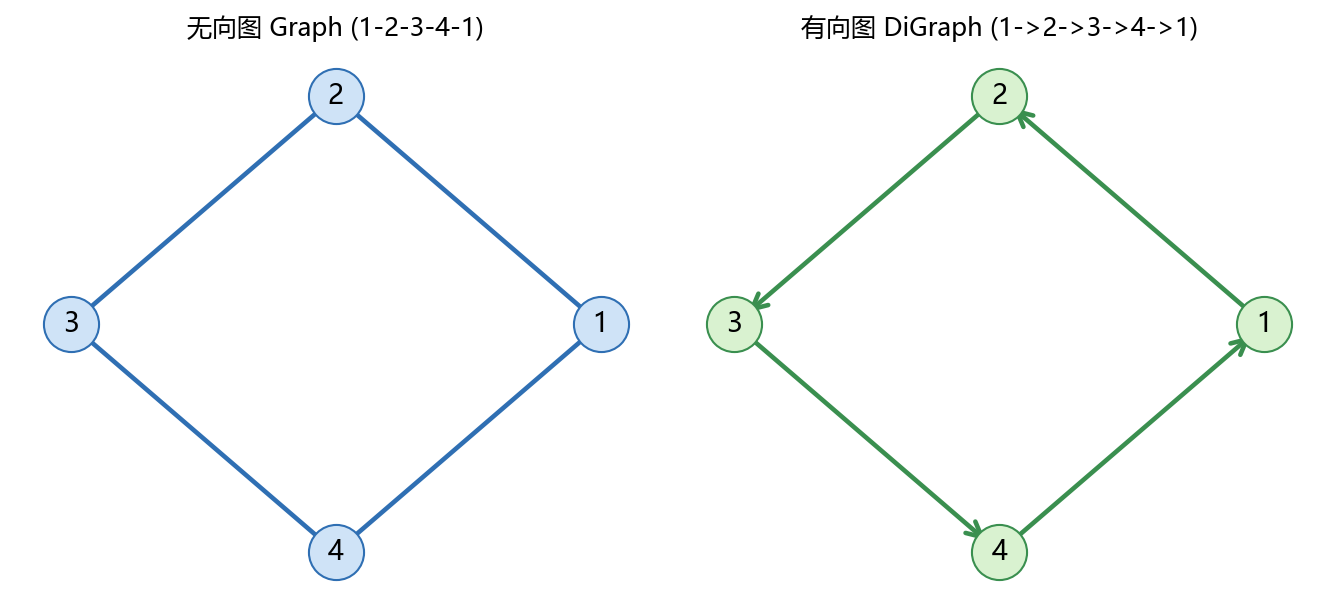
\includegraphics[keepaspectratio,alt={无向图与有向图示例}]{figures/06-networkx/graph_basic.png}}
\caption{无向图与有向图示例}
\end{figure}

\begin{center}\rule{0.5\linewidth}{0.5pt}\end{center}

\subsection{1.3
创建有向图（DiGraph）}\label{ux521bux5efaux6709ux5411ux56fedigraph}

有向图的边有方向，用 nx.DiGraph 创建。

\begin{Shaded}
\begin{Highlighting}[]
\ImportTok{import}\NormalTok{ networkx }\ImportTok{as}\NormalTok{ nx}

\NormalTok{DG }\OperatorTok{=}\NormalTok{ nx.DiGraph()}
\NormalTok{DG.add\_node(}\DecValTok{1}\NormalTok{)}
\NormalTok{DG.add\_nodes\_from([}\DecValTok{2}\NormalTok{, }\DecValTok{3}\NormalTok{, }\DecValTok{4}\NormalTok{])}
\NormalTok{DG.add\_edge(}\DecValTok{1}\NormalTok{, }\DecValTok{2}\NormalTok{)}
\NormalTok{DG.add\_edges\_from([(}\DecValTok{2}\NormalTok{, }\DecValTok{3}\NormalTok{), (}\DecValTok{3}\NormalTok{, }\DecValTok{4}\NormalTok{), (}\DecValTok{4}\NormalTok{, }\DecValTok{1}\NormalTok{)])}

\BuiltInTok{print}\NormalTok{(DG.nodes())}
\BuiltInTok{print}\NormalTok{(DG.edges())}
\end{Highlighting}
\end{Shaded}

\begin{Shaded}
\begin{Highlighting}[]
\NormalTok{[1, 2, 3, 4]}
\NormalTok{[(1, 2), (2, 3), (3, 4), (4, 1)]}
\end{Highlighting}
\end{Shaded}

\subsubsection{1.3.1
入度、出度、前驱与后继}\label{ux5165ux5ea6ux51faux5ea6ux524dux9a71ux4e0eux540eux7ee7}

\begin{Shaded}
\begin{Highlighting}[]
\BuiltInTok{print}\NormalTok{(DG.in\_degree())}
\BuiltInTok{print}\NormalTok{(DG.out\_degree())}
\ControlFlowTok{for}\NormalTok{ node }\KeywordTok{in}\NormalTok{ DG.nodes():}
    \BuiltInTok{print}\NormalTok{(}\StringTok{"Node"}\NormalTok{, node, }\StringTok{"in{-}degree"}\NormalTok{, DG.in\_degree(node), }\StringTok{"out{-}degree"}\NormalTok{, DG.out\_degree(node))}
\BuiltInTok{print}\NormalTok{(}\BuiltInTok{list}\NormalTok{(DG.predecessors(}\DecValTok{2}\NormalTok{)))   }\CommentTok{\# 指向 2 的节点}
\BuiltInTok{print}\NormalTok{(}\BuiltInTok{list}\NormalTok{(DG.successors(}\DecValTok{2}\NormalTok{)))     }\CommentTok{\# 2 指向的节点}
\end{Highlighting}
\end{Shaded}

\begin{Shaded}
\begin{Highlighting}[]
\NormalTok{[(1, 1), (2, 1), (3, 1), (4, 1)]}
\NormalTok{[(1, 1), (2, 1), (3, 1), (4, 1)]}
\NormalTok{Node 1 in{-}degree 1 out{-}degree 1}
\NormalTok{Node 2 in{-}degree 1 out{-}degree 1}
\NormalTok{Node 3 in{-}degree 1 out{-}degree 1}
\NormalTok{Node 4 in{-}degree 1 out{-}degree 1}
\NormalTok{[1]}
\NormalTok{[3]}
\end{Highlighting}
\end{Shaded}

\begin{quote}
注意：原始资料里用 zip(nodes, in\_degree, out\_degree)
的写法会把元组拆错（in\_degree 返回的是 (节点, 度数)
对）。建议像上面这样用 DG.in\_degree(node) 单独取度数，或用
dict(DG.in\_degree())。
\end{quote}

\subsubsection{1.3.2
强连通与弱连通}\label{ux5f3aux8fdeux901aux4e0eux5f31ux8fdeux901a}

有向图的连通性要区分：

\begin{itemize}
\tightlist
\item
  强连通：任意两点都互相可达；
\item
  弱连通：忽略方向后，任意两点可达。
\end{itemize}

\begin{Shaded}
\begin{Highlighting}[]
\BuiltInTok{print}\NormalTok{(nx.is\_strongly\_connected(DG))}
\BuiltInTok{print}\NormalTok{(nx.is\_weakly\_connected(DG))}
\end{Highlighting}
\end{Shaded}

\begin{Shaded}
\begin{Highlighting}[]
\NormalTok{True}
\NormalTok{True}
\end{Highlighting}
\end{Shaded}

\subsubsection{1.3.3 有向图遍历}\label{ux6709ux5411ux56feux904dux5386}

\begin{Shaded}
\begin{Highlighting}[]
\BuiltInTok{print}\NormalTok{(}\BuiltInTok{list}\NormalTok{(nx.dfs\_preorder\_nodes(DG, source}\OperatorTok{=}\DecValTok{1}\NormalTok{)))}
\BuiltInTok{print}\NormalTok{(}\BuiltInTok{list}\NormalTok{(nx.bfs\_edges(DG, source}\OperatorTok{=}\DecValTok{1}\NormalTok{)))}
\end{Highlighting}
\end{Shaded}

\begin{Shaded}
\begin{Highlighting}[]
\NormalTok{[1, 2, 3, 4]}
\NormalTok{[(1, 2), (2, 3), (3, 4)]}
\end{Highlighting}
\end{Shaded}

绘图时 NetworkX 会根据有向性画箭头：

\begin{Shaded}
\begin{Highlighting}[]
\ImportTok{import}\NormalTok{ matplotlib.pyplot }\ImportTok{as}\NormalTok{ plt}
\NormalTok{nx.draw(DG, with\_labels}\OperatorTok{=}\VariableTok{True}\NormalTok{, font\_weight}\OperatorTok{=}\StringTok{"bold"}\NormalTok{, arrowstyle}\OperatorTok{=}\StringTok{"{-}\textgreater{}"}\NormalTok{, arrowsize}\OperatorTok{=}\DecValTok{20}\NormalTok{)}
\NormalTok{plt.show()}
\end{Highlighting}
\end{Shaded}

\begin{center}\rule{0.5\linewidth}{0.5pt}\end{center}

\subsection{1.4
节点与边属性、加权图}\label{ux8282ux70b9ux4e0eux8fb9ux5c5eux6027ux52a0ux6743ux56fe}

\subsubsection{1.4.1 权重（weight）}\label{ux6743ux91cdweight}

\begin{Shaded}
\begin{Highlighting}[]
\NormalTok{G }\OperatorTok{=}\NormalTok{ nx.Graph()}
\NormalTok{G.add\_weighted\_edges\_from([(}\StringTok{"A"}\NormalTok{, }\StringTok{"B"}\NormalTok{, }\DecValTok{10}\NormalTok{), (}\StringTok{"A"}\NormalTok{, }\StringTok{"C"}\NormalTok{, }\DecValTok{6}\NormalTok{), (}\StringTok{"B"}\NormalTok{, }\StringTok{"C"}\NormalTok{, }\DecValTok{5}\NormalTok{)])}
\BuiltInTok{print}\NormalTok{(}\BuiltInTok{list}\NormalTok{(G.edges(data}\OperatorTok{=}\VariableTok{True}\NormalTok{)))}
\BuiltInTok{print}\NormalTok{(G[}\StringTok{"A"}\NormalTok{][}\StringTok{"B"}\NormalTok{])                    }\CommentTok{\# 取出 A{-}B 边的属性字典}
\BuiltInTok{print}\NormalTok{(G.degree())                     }\CommentTok{\# 普通度}
\BuiltInTok{print}\NormalTok{(G.degree(weight}\OperatorTok{=}\StringTok{"weight"}\NormalTok{))      }\CommentTok{\# 加权度（点强度）}
\end{Highlighting}
\end{Shaded}

\begin{Shaded}
\begin{Highlighting}[]
\NormalTok{[(\textquotesingle{}A\textquotesingle{}, \textquotesingle{}B\textquotesingle{}, \{\textquotesingle{}weight\textquotesingle{}: 10\}), (\textquotesingle{}A\textquotesingle{}, \textquotesingle{}C\textquotesingle{}, \{\textquotesingle{}weight\textquotesingle{}: 6\}), (\textquotesingle{}B\textquotesingle{}, \textquotesingle{}C\textquotesingle{}, \{\textquotesingle{}weight\textquotesingle{}: 5\})]}
\NormalTok{\{\textquotesingle{}weight\textquotesingle{}: 10\}}
\NormalTok{[(\textquotesingle{}A\textquotesingle{}, 2), (\textquotesingle{}B\textquotesingle{}, 2), (\textquotesingle{}C\textquotesingle{}, 2)]}
\NormalTok{[(\textquotesingle{}A\textquotesingle{}, 16), (\textquotesingle{}B\textquotesingle{}, 15), (\textquotesingle{}C\textquotesingle{}, 11)]}
\end{Highlighting}
\end{Shaded}

\begin{quote}
点强度（weighted degree）是节点所有相连边的权重和：A 连
B(10)、C(6)，所以是 16。加权网络上``重要节点''的衡量常从点强度出发。
\end{quote}

\subsubsection{1.4.2 节点属性}\label{ux8282ux70b9ux5c5eux6027}

\begin{Shaded}
\begin{Highlighting}[]
\NormalTok{G.add\_node(}\StringTok{"A"}\NormalTok{, role}\OperatorTok{=}\StringTok{"hub"}\NormalTok{, color}\OperatorTok{=}\StringTok{"red"}\NormalTok{)}
\BuiltInTok{print}\NormalTok{(}\BuiltInTok{list}\NormalTok{(G.nodes(data}\OperatorTok{=}\VariableTok{True}\NormalTok{)))}
\end{Highlighting}
\end{Shaded}

\begin{Shaded}
\begin{Highlighting}[]
\NormalTok{[(\textquotesingle{}A\textquotesingle{}, \{\textquotesingle{}role\textquotesingle{}: \textquotesingle{}hub\textquotesingle{}, \textquotesingle{}color\textquotesingle{}: \textquotesingle{}red\textquotesingle{}\}), (\textquotesingle{}B\textquotesingle{}, \{\}), (\textquotesingle{}C\textquotesingle{}, \{\})]}
\end{Highlighting}
\end{Shaded}

节点/边上可以挂任意字典属性；用 G.nodes(data=True) 与 G.edges(data=True)
一起查看。

\begin{center}\rule{0.5\linewidth}{0.5pt}\end{center}

\subsection{1.5
常用图生成器}\label{ux5e38ux7528ux56feux751fux6210ux5668}

NetworkX 自带许多``造图''模板，适合课堂演示与随机网络实验。

\begin{Shaded}
\begin{Highlighting}[]
\BuiltInTok{print}\NormalTok{(}\BuiltInTok{list}\NormalTok{(nx.path\_graph(}\DecValTok{6}\NormalTok{).edges()))}
\BuiltInTok{print}\NormalTok{(}\BuiltInTok{list}\NormalTok{(nx.cycle\_graph(}\DecValTok{5}\NormalTok{).edges()))}
\BuiltInTok{print}\NormalTok{(}\BuiltInTok{list}\NormalTok{(nx.complete\_graph(}\DecValTok{4}\NormalTok{).edges()))}
\BuiltInTok{print}\NormalTok{(}\BuiltInTok{list}\NormalTok{(nx.star\_graph(}\DecValTok{5}\NormalTok{).edges()))}
\BuiltInTok{print}\NormalTok{(}\BuiltInTok{list}\NormalTok{(nx.grid\_2d\_graph(}\DecValTok{2}\NormalTok{, }\DecValTok{3}\NormalTok{).nodes()))}
\BuiltInTok{print}\NormalTok{(}\BuiltInTok{list}\NormalTok{(nx.grid\_2d\_graph(}\DecValTok{2}\NormalTok{, }\DecValTok{3}\NormalTok{).edges()))}
\NormalTok{K }\OperatorTok{=}\NormalTok{ nx.karate\_club\_graph()}
\BuiltInTok{print}\NormalTok{(}\StringTok{"karate\_club:"}\NormalTok{, K.number\_of\_nodes(), K.number\_of\_edges())}
\end{Highlighting}
\end{Shaded}

\begin{Shaded}
\begin{Highlighting}[]
\NormalTok{[(0, 1), (1, 2), (2, 3), (3, 4), (4, 5)]}
\NormalTok{[(0, 1), (0, 4), (1, 2), (2, 3), (3, 4)]}
\NormalTok{[(0, 1), (0, 2), (0, 3), (1, 2), (1, 3), (2, 3)]}
\NormalTok{[(0, 1), (0, 2), (0, 3), (0, 4), (0, 5)]}
\NormalTok{[(0, 0), (0, 1), (0, 2), (1, 0), (1, 1), (1, 2)]}
\NormalTok{[((0, 0), (1, 0)), ((0, 0), (0, 1)), ((0, 1), (1, 1)), ((0, 1), (0, 2)), ((0, 2), (1, 2)), ((1, 0), (1, 1)), ((1, 1), (1, 2))]}
\NormalTok{karate\_club: 34 78}
\end{Highlighting}
\end{Shaded}

随机网络生成器通常带 seed 参数，保证结果可复现：

\begin{Shaded}
\begin{Highlighting}[]
\NormalTok{er }\OperatorTok{=}\NormalTok{ nx.erdos\_renyi\_graph(}\DecValTok{10}\NormalTok{, }\FloatTok{0.3}\NormalTok{, seed}\OperatorTok{=}\DecValTok{42}\NormalTok{)}
\NormalTok{ws }\OperatorTok{=}\NormalTok{ nx.watts\_strogatz\_graph(}\DecValTok{10}\NormalTok{, }\DecValTok{4}\NormalTok{, }\FloatTok{0.1}\NormalTok{, seed}\OperatorTok{=}\DecValTok{42}\NormalTok{)}
\NormalTok{ba }\OperatorTok{=}\NormalTok{ nx.barabasi\_albert\_graph(}\DecValTok{10}\NormalTok{, }\DecValTok{2}\NormalTok{, seed}\OperatorTok{=}\DecValTok{42}\NormalTok{)}
\BuiltInTok{print}\NormalTok{(}\StringTok{"erdos\_renyi:"}\NormalTok{, er.number\_of\_nodes(), er.number\_of\_edges())}
\BuiltInTok{print}\NormalTok{(}\StringTok{"watts\_strogatz:"}\NormalTok{, ws.number\_of\_nodes(), ws.number\_of\_edges())}
\BuiltInTok{print}\NormalTok{(}\StringTok{"barabasi\_albert:"}\NormalTok{, ba.number\_of\_nodes(), ba.number\_of\_edges())}
\end{Highlighting}
\end{Shaded}

\begin{Shaded}
\begin{Highlighting}[]
\NormalTok{erdos\_renyi: 10 17}
\NormalTok{watts\_strogatz: 10 20}
\NormalTok{barabasi\_albert: 10 16}
\end{Highlighting}
\end{Shaded}

\begin{center}\rule{0.5\linewidth}{0.5pt}\end{center}

\subsection{1.6 邻接矩阵（与 NumPy
对接）}\label{ux90bbux63a5ux77e9ux9635ux4e0e-numpy-ux5bf9ux63a5}

用 nx.to\_numpy\_array 可把图转成邻接矩阵，便于交给 NumPy/SciPy
做数值计算。

\begin{Shaded}
\begin{Highlighting}[]
\ImportTok{import}\NormalTok{ numpy }\ImportTok{as}\NormalTok{ np}
\NormalTok{G }\OperatorTok{=}\NormalTok{ nx.Graph()}
\NormalTok{G.add\_edges\_from([(}\DecValTok{1}\NormalTok{, }\DecValTok{2}\NormalTok{), (}\DecValTok{2}\NormalTok{, }\DecValTok{3}\NormalTok{), (}\DecValTok{3}\NormalTok{, }\DecValTok{1}\NormalTok{), (}\DecValTok{3}\NormalTok{, }\DecValTok{4}\NormalTok{)])}
\NormalTok{A }\OperatorTok{=}\NormalTok{ nx.to\_numpy\_array(G)}
\BuiltInTok{print}\NormalTok{(A)}
\end{Highlighting}
\end{Shaded}

\begin{Shaded}
\begin{Highlighting}[]
\NormalTok{[[0. 1. 1. 0.]}
\NormalTok{ [1. 0. 1. 0.]}
\NormalTok{ [1. 1. 0. 1.]}
\NormalTok{ [0. 0. 1. 0.]]}
\end{Highlighting}
\end{Shaded}

有向图会得到非对称矩阵：

\begin{Shaded}
\begin{Highlighting}[]
\NormalTok{D }\OperatorTok{=}\NormalTok{ nx.DiGraph()}\OperatorTok{;}\NormalTok{ D.add\_edges\_from([(}\DecValTok{1}\NormalTok{, }\DecValTok{2}\NormalTok{), (}\DecValTok{2}\NormalTok{, }\DecValTok{3}\NormalTok{), (}\DecValTok{3}\NormalTok{, }\DecValTok{1}\NormalTok{), (}\DecValTok{2}\NormalTok{, }\DecValTok{4}\NormalTok{)])}
\BuiltInTok{print}\NormalTok{(nx.to\_numpy\_array(D))}
\end{Highlighting}
\end{Shaded}

\begin{Shaded}
\begin{Highlighting}[]
\NormalTok{[[0. 1. 0. 0.]}
\NormalTok{ [0. 0. 1. 1.]}
\NormalTok{ [1. 0. 0. 0.]}
\NormalTok{ [0. 0. 0. 0.]]}
\end{Highlighting}
\end{Shaded}

\subsection{案例卡 1：用 nx.Graph
建``班级社交网''------节点/边/属性/度}\label{ux6848ux4f8bux5361-1ux7528-nx.graph-ux5efaux73edux7ea7ux793eux4ea4ux7f51ux8282ux70b9ux8fb9ux5c5eux6027ux5ea6}

\subsubsection{目标}\label{ux76eeux6807-24}

把 5 位同学当成``节点''，把``一起学习/讨论''当成``边''，用
\texttt{nx.Graph}
建一张班级社交网。你会顺带掌握：给节点挂属性、给边加权重（每周讨论次数）、看每个节点的\textbf{度}（直接朋友数）与\textbf{点强度}（加权度=朋友往来总次数）。

\subsubsection{代码}\label{ux4ee3ux7801-25}

\begin{Shaded}
\begin{Highlighting}[]
\ImportTok{import}\NormalTok{ networkx }\ImportTok{as}\NormalTok{ nx}
\ImportTok{import}\NormalTok{ matplotlib.pyplot }\ImportTok{as}\NormalTok{ plt}
\ImportTok{import}\NormalTok{ numpy }\ImportTok{as}\NormalTok{ np}
\ImportTok{import}\NormalTok{ os}

\NormalTok{plt.rcParams[}\StringTok{\textquotesingle{}font.sans{-}serif\textquotesingle{}}\NormalTok{] }\OperatorTok{=}\NormalTok{ [}\StringTok{\textquotesingle{}Microsoft YaHei\textquotesingle{}}\NormalTok{, }\StringTok{\textquotesingle{}SimHei\textquotesingle{}}\NormalTok{, }\StringTok{\textquotesingle{}DejaVu Sans\textquotesingle{}}\NormalTok{]}
\NormalTok{plt.rcParams[}\StringTok{\textquotesingle{}axes.unicode\_minus\textquotesingle{}}\NormalTok{] }\OperatorTok{=} \VariableTok{False}
\NormalTok{np.set\_printoptions(precision}\OperatorTok{=}\DecValTok{4}\NormalTok{, suppress}\OperatorTok{=}\VariableTok{True}\NormalTok{)}

\CommentTok{\#\# 1) 建空图}
\NormalTok{G }\OperatorTok{=}\NormalTok{ nx.Graph()}

\CommentTok{\#\# 2) 一次加多个节点，并给每个节点挂属性(班级/兴趣)}
\NormalTok{students }\OperatorTok{=}\NormalTok{ [}
\NormalTok{    (}\StringTok{\textquotesingle{}小明\textquotesingle{}}\NormalTok{, \{}\StringTok{\textquotesingle{}cls\textquotesingle{}}\NormalTok{: }\StringTok{\textquotesingle{}一班\textquotesingle{}}\NormalTok{, }\StringTok{\textquotesingle{}interest\textquotesingle{}}\NormalTok{: }\StringTok{\textquotesingle{}数学\textquotesingle{}}\NormalTok{\}),}
\NormalTok{    (}\StringTok{\textquotesingle{}小红\textquotesingle{}}\NormalTok{, \{}\StringTok{\textquotesingle{}cls\textquotesingle{}}\NormalTok{: }\StringTok{\textquotesingle{}一班\textquotesingle{}}\NormalTok{, }\StringTok{\textquotesingle{}interest\textquotesingle{}}\NormalTok{: }\StringTok{\textquotesingle{}编程\textquotesingle{}}\NormalTok{\}),}
\NormalTok{    (}\StringTok{\textquotesingle{}小刚\textquotesingle{}}\NormalTok{, \{}\StringTok{\textquotesingle{}cls\textquotesingle{}}\NormalTok{: }\StringTok{\textquotesingle{}一班\textquotesingle{}}\NormalTok{, }\StringTok{\textquotesingle{}interest\textquotesingle{}}\NormalTok{: }\StringTok{\textquotesingle{}物理\textquotesingle{}}\NormalTok{\}),}
\NormalTok{    (}\StringTok{\textquotesingle{}小丽\textquotesingle{}}\NormalTok{, \{}\StringTok{\textquotesingle{}cls\textquotesingle{}}\NormalTok{: }\StringTok{\textquotesingle{}二班\textquotesingle{}}\NormalTok{, }\StringTok{\textquotesingle{}interest\textquotesingle{}}\NormalTok{: }\StringTok{\textquotesingle{}语文\textquotesingle{}}\NormalTok{\}),}
\NormalTok{    (}\StringTok{\textquotesingle{}小华\textquotesingle{}}\NormalTok{, \{}\StringTok{\textquotesingle{}cls\textquotesingle{}}\NormalTok{: }\StringTok{\textquotesingle{}二班\textquotesingle{}}\NormalTok{, }\StringTok{\textquotesingle{}interest\textquotesingle{}}\NormalTok{: }\StringTok{\textquotesingle{}美术\textquotesingle{}}\NormalTok{\}),}
\NormalTok{]}
\NormalTok{G.add\_nodes\_from(students)}

\CommentTok{\#\# 3) 加边，weight 表示每周一起讨论的次数}
\NormalTok{G.add\_weighted\_edges\_from([}
\NormalTok{    (}\StringTok{\textquotesingle{}小明\textquotesingle{}}\NormalTok{, }\StringTok{\textquotesingle{}小红\textquotesingle{}}\NormalTok{, }\DecValTok{3}\NormalTok{),}
\NormalTok{    (}\StringTok{\textquotesingle{}小明\textquotesingle{}}\NormalTok{, }\StringTok{\textquotesingle{}小刚\textquotesingle{}}\NormalTok{, }\DecValTok{2}\NormalTok{),}
\NormalTok{    (}\StringTok{\textquotesingle{}小红\textquotesingle{}}\NormalTok{, }\StringTok{\textquotesingle{}小刚\textquotesingle{}}\NormalTok{, }\DecValTok{4}\NormalTok{),}
\NormalTok{    (}\StringTok{\textquotesingle{}小刚\textquotesingle{}}\NormalTok{, }\StringTok{\textquotesingle{}小丽\textquotesingle{}}\NormalTok{, }\DecValTok{1}\NormalTok{),}
\NormalTok{    (}\StringTok{\textquotesingle{}小丽\textquotesingle{}}\NormalTok{, }\StringTok{\textquotesingle{}小华\textquotesingle{}}\NormalTok{, }\DecValTok{5}\NormalTok{),}
\NormalTok{])}

\BuiltInTok{print}\NormalTok{(}\StringTok{\textquotesingle{}节点数:\textquotesingle{}}\NormalTok{, G.number\_of\_nodes(), }\StringTok{\textquotesingle{}  边数:\textquotesingle{}}\NormalTok{, G.number\_of\_edges())}
\BuiltInTok{print}\NormalTok{(}\StringTok{\textquotesingle{}节点及属性:\textquotesingle{}}\NormalTok{)}
\ControlFlowTok{for}\NormalTok{ n, data }\KeywordTok{in}\NormalTok{ G.nodes(data}\OperatorTok{=}\VariableTok{True}\NormalTok{):}
    \BuiltInTok{print}\NormalTok{(}\StringTok{\textquotesingle{} \textquotesingle{}}\NormalTok{, n, data)}
\BuiltInTok{print}\NormalTok{(}\StringTok{\textquotesingle{}边及权重:\textquotesingle{}}\NormalTok{)}
\ControlFlowTok{for}\NormalTok{ u, v, w }\KeywordTok{in}\NormalTok{ G.edges(data}\OperatorTok{=}\StringTok{\textquotesingle{}weight\textquotesingle{}}\NormalTok{):}
    \BuiltInTok{print}\NormalTok{(}\SpecialStringTok{f\textquotesingle{}  }\SpecialCharTok{\{}\NormalTok{u}\SpecialCharTok{\}}\SpecialStringTok{ {-}{-} }\SpecialCharTok{\{}\NormalTok{v}\SpecialCharTok{\}}\SpecialStringTok{ : }\SpecialCharTok{\{}\NormalTok{w}\SpecialCharTok{\}}\SpecialStringTok{\textquotesingle{}}\NormalTok{)}

\CommentTok{\#\# 4) 度 与 点强度(加权度)}
\BuiltInTok{print}\NormalTok{(}\StringTok{\textquotesingle{}每个节点的度(降序):\textquotesingle{}}\NormalTok{, }\BuiltInTok{sorted}\NormalTok{(}\BuiltInTok{dict}\NormalTok{(G.degree()).items(), key}\OperatorTok{=}\KeywordTok{lambda}\NormalTok{ x: (}\OperatorTok{{-}}\NormalTok{x[}\DecValTok{1}\NormalTok{], x[}\DecValTok{0}\NormalTok{])))}
\BuiltInTok{print}\NormalTok{(}\StringTok{\textquotesingle{}每个节点的加权度/点强度(降序):\textquotesingle{}}\NormalTok{,}
      \BuiltInTok{sorted}\NormalTok{(}\BuiltInTok{dict}\NormalTok{(G.degree(weight}\OperatorTok{=}\StringTok{\textquotesingle{}weight\textquotesingle{}}\NormalTok{)).items(), key}\OperatorTok{=}\KeywordTok{lambda}\NormalTok{ x: (}\OperatorTok{{-}}\NormalTok{x[}\DecValTok{1}\NormalTok{], x[}\DecValTok{0}\NormalTok{])))}

\CommentTok{\#\# 5) 画出来(jupyter 里可直接显示；脚本环境保存到 figures/06{-}networkx/)}
\NormalTok{os.makedirs(}\StringTok{\textquotesingle{}images\textquotesingle{}}\NormalTok{, exist\_ok}\OperatorTok{=}\VariableTok{True}\NormalTok{)}
\NormalTok{pos }\OperatorTok{=}\NormalTok{ nx.spring\_layout(G, seed}\OperatorTok{=}\DecValTok{42}\NormalTok{, k}\OperatorTok{=}\FloatTok{0.8}\NormalTok{)}
\NormalTok{plt.figure(figsize}\OperatorTok{=}\NormalTok{(}\FloatTok{6.4}\NormalTok{, }\FloatTok{4.6}\NormalTok{))}
\NormalTok{nx.draw\_networkx\_nodes(G, pos, node\_size}\OperatorTok{=}\DecValTok{800}\NormalTok{, node\_color}\OperatorTok{=}\StringTok{\textquotesingle{}\#cfe3f7\textquotesingle{}}\NormalTok{, edgecolors}\OperatorTok{=}\StringTok{\textquotesingle{}\#2f6fb3\textquotesingle{}}\NormalTok{)}
\NormalTok{nx.draw\_networkx\_edges(G, pos, width}\OperatorTok{=}\FloatTok{2.0}\NormalTok{, edge\_color}\OperatorTok{=}\StringTok{\textquotesingle{}\#4b8bbe\textquotesingle{}}\NormalTok{)}
\NormalTok{nx.draw\_networkx\_labels(G, pos, font\_size}\OperatorTok{=}\DecValTok{11}\NormalTok{, font\_family}\OperatorTok{=}\StringTok{\textquotesingle{}Microsoft YaHei\textquotesingle{}}\NormalTok{)}
\NormalTok{plt.title(}\StringTok{\textquotesingle{}班级社交网\textquotesingle{}}\NormalTok{)}
\NormalTok{plt.axis(}\StringTok{\textquotesingle{}off\textquotesingle{}}\NormalTok{)}
\NormalTok{plt.tight\_layout()}
\NormalTok{plt.savefig(}\StringTok{\textquotesingle{}figures/06{-}networkx/case1\_class\_network.png\textquotesingle{}}\NormalTok{, dpi}\OperatorTok{=}\DecValTok{150}\NormalTok{)}
\BuiltInTok{print}\NormalTok{(}\StringTok{\textquotesingle{}已保存 figures/06{-}networkx/case1\_class\_network.png\textquotesingle{}}\NormalTok{)}
\NormalTok{plt.close()}
\end{Highlighting}
\end{Shaded}

\subsubsection{运行结果(已运行核验)}\label{ux8fd0ux884cux7ed3ux679cux5df2ux8fd0ux884cux6838ux9a8c-23}

\begin{Shaded}
\begin{Highlighting}[]
\NormalTok{节点数: 5   边数: 5}
\NormalTok{节点及属性:}
\NormalTok{  小明 \{\textquotesingle{}cls\textquotesingle{}: \textquotesingle{}一班\textquotesingle{}, \textquotesingle{}interest\textquotesingle{}: \textquotesingle{}数学\textquotesingle{}\}}
\NormalTok{  小红 \{\textquotesingle{}cls\textquotesingle{}: \textquotesingle{}一班\textquotesingle{}, \textquotesingle{}interest\textquotesingle{}: \textquotesingle{}编程\textquotesingle{}\}}
\NormalTok{  小刚 \{\textquotesingle{}cls\textquotesingle{}: \textquotesingle{}一班\textquotesingle{}, \textquotesingle{}interest\textquotesingle{}: \textquotesingle{}物理\textquotesingle{}\}}
\NormalTok{  小丽 \{\textquotesingle{}cls\textquotesingle{}: \textquotesingle{}二班\textquotesingle{}, \textquotesingle{}interest\textquotesingle{}: \textquotesingle{}语文\textquotesingle{}\}}
\NormalTok{  小华 \{\textquotesingle{}cls\textquotesingle{}: \textquotesingle{}二班\textquotesingle{}, \textquotesingle{}interest\textquotesingle{}: \textquotesingle{}美术\textquotesingle{}\}}
\NormalTok{边及权重:}
\NormalTok{  小明 {-}{-} 小红 : 3}
\NormalTok{  小明 {-}{-} 小刚 : 2}
\NormalTok{  小红 {-}{-} 小刚 : 4}
\NormalTok{  小刚 {-}{-} 小丽 : 1}
\NormalTok{  小丽 {-}{-} 小华 : 5}
\NormalTok{每个节点的度(降序): [(\textquotesingle{}小刚\textquotesingle{}, 3), (\textquotesingle{}小丽\textquotesingle{}, 2), (\textquotesingle{}小明\textquotesingle{}, 2), (\textquotesingle{}小红\textquotesingle{}, 2), (\textquotesingle{}小华\textquotesingle{}, 1)]}
\NormalTok{每个节点的加权度/点强度(降序): [(\textquotesingle{}小刚\textquotesingle{}, 7), (\textquotesingle{}小红\textquotesingle{}, 7), (\textquotesingle{}小丽\textquotesingle{}, 6), (\textquotesingle{}小华\textquotesingle{}, 5), (\textquotesingle{}小明\textquotesingle{}, 5)]}
\NormalTok{已保存 figures/06{-}networkx/case1\_class\_network.png}
\end{Highlighting}
\end{Shaded}

\subsubsection{讲解}\label{ux8bb2ux89e3-23}

\textbf{一句话解释}：先画一张``人=点、一起学习=连线''的网；每条线还能记一个数（每周讨论几次），这样不但知道``谁朋友多''，还知道``谁和朋友来往最勤''。

\begin{enumerate}
\def\labelenumi{\arabic{enumi}.}
\tightlist
\item
  \texttt{G\ =\ nx.Graph()} 建一张\textbf{无向图}：朋友关系不分方向，A
  和 B 是朋友就等于 B 和 A 是朋友。
\item
  \texttt{G.add\_nodes\_from(students)} 里每个元素是
  \texttt{(节点名,\ 属性字典)}，所以一次就能把``班级、兴趣''挂在节点上；查看时用
  \texttt{G.nodes(data=True)} 会得到 \texttt{(节点,\ 属性字典)} 对。
\item
  \texttt{G.add\_weighted\_edges\_from(...)} 的每个元素是
  \texttt{(起点,\ 终点,\ 权重)}；\texttt{weight} 是 NetworkX
  约定好的边属性名，后面
  \texttt{degree(weight=\textquotesingle{}weight\textquotesingle{})}
  才能自动读到它。
\item
  \texttt{G.degree()} 是\textbf{直接邻居数}：小明连小红、小刚，所以是
  2；小刚连小明、小红、小丽，是 3。
\item
  \texttt{G.degree(weight=\textquotesingle{}weight\textquotesingle{})}
  是把``每条边的权重相加''，等于\textbf{点强度}：小刚=2+4+1=7，小红=3+4=7，小丽=1+5=6，小华=5，小明=3+2=5。所以小刚虽然度最高，但``来往总次数''第一的是小刚和小红并列。
\item
  \texttt{nx.spring\_layout(G,\ seed=42)} 给节点随机选初始位置，固定
  \texttt{seed=42} 才能每次画出同一张布局；保存到
  \texttt{figures/06-networkx/} 前先
  \texttt{os.makedirs(\textquotesingle{}images\textquotesingle{},\ exist\_ok=True)}，避免目录不存在报错。
\end{enumerate}

\begin{figure}
\centering
\pandocbounded{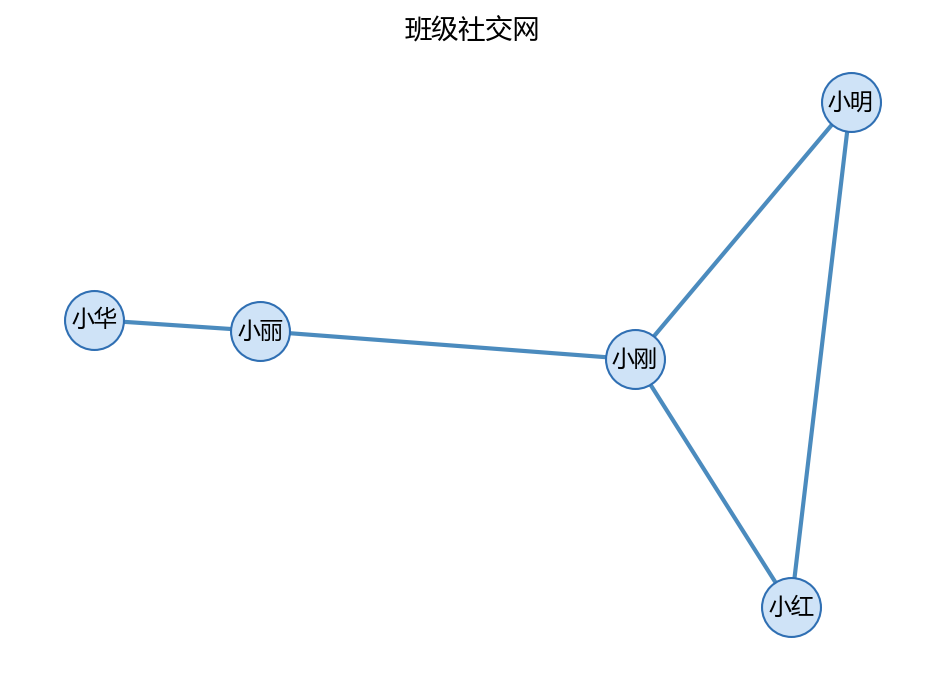
\includegraphics[keepaspectratio,alt={班级社交网}]{figures/06-networkx/case1_class_network.png}}
\caption{班级社交网}
\end{figure}

\subsubsection{主要用法 / API}\label{ux4e3bux8981ux7528ux6cd5-api-24}

{\def\LTcaptype{none} % do not increment counter
\begin{longtable}[]{@{}
  >{\raggedright\arraybackslash}p{(\linewidth - 4\tabcolsep) * \real{0.3333}}
  >{\raggedright\arraybackslash}p{(\linewidth - 4\tabcolsep) * \real{0.3333}}
  >{\raggedright\arraybackslash}p{(\linewidth - 4\tabcolsep) * \real{0.3333}}@{}}
\toprule\noalign{}
\begin{minipage}[b]{\linewidth}\raggedright
需求
\end{minipage} & \begin{minipage}[b]{\linewidth}\raggedright
写法
\end{minipage} & \begin{minipage}[b]{\linewidth}\raggedright
说明
\end{minipage} \\
\midrule\noalign{}
\endhead
\bottomrule\noalign{}
\endlastfoot
建空无向图 & \texttt{nx.Graph()} & 边无方向 \\
加单个/多个节点 & \texttt{add\_node} / \texttt{add\_nodes\_from} &
可带属性 \\
加单条/多条边 & \texttt{add\_edge} / \texttt{add\_edges\_from} &
无向图自动补反向 \\
加带权边 & \texttt{add\_weighted\_edges\_from({[}(u,\ v,\ w){]})} &
属性名 \texttt{weight} \\
查看节点/边属性 & \texttt{G.nodes(data=True)} /
\texttt{G.edges(data=True)} & 得到 \texttt{(节点,\ dict)} /
\texttt{(u,\ v,\ dict)} \\
度 & \texttt{G.degree()} / \texttt{G.degree(node)} & 直接邻居数 \\
点强度 &
\texttt{G.degree(weight=\textquotesingle{}weight\textquotesingle{})} &
加权度 \\
画图 & \texttt{nx.draw\_networkx\_*} + \texttt{plt.savefig} &
需配中文字体 \\
\end{longtable}
}

\subsubsection{常见错误}\label{ux5e38ux89c1ux9519ux8bef-24}

\begin{enumerate}
\def\labelenumi{\arabic{enumi}.}
\tightlist
\item
  以为 \texttt{add\_edge(u,\ v,\ 10)} 的第三个参数是权重 → 错误；正解是
  \texttt{add\_edge(u,\ v,\ weight=10)} 或
  \texttt{add\_weighted\_edges\_from}。
\item
  忘记
  \texttt{G.degree(weight=\textquotesingle{}weight\textquotesingle{})}
  的 \texttt{weight} 参数名要跟边属性名一致；如果边属性叫
  \texttt{time}，就要写
  \texttt{weight=\textquotesingle{}time\textquotesingle{}}。
\item
  用 \texttt{plt.show()} 在无界面环境会卡住/无反应 → 脚本/作业里用
  \texttt{plt.savefig(...)}；\texttt{spring\_layout} 不传 \texttt{seed}
  每次布局都不同，作业截图容易对不上。
\item
  \texttt{sorted(G.degree())} 返回的是按节点名排列的
  \texttt{(节点,\ 度)} 列表；想按度数排序要
  \texttt{key=lambda\ x:\ (-x{[}1{]},\ x{[}0{]})}。
\end{enumerate}

\subsubsection{拓展 / 跟练}\label{ux62d3ux5c55-ux8ddfux7ec3-12}

\begin{enumerate}
\def\labelenumi{\arabic{enumi}.}
\tightlist
\item
  新加一位同学 \texttt{小强} 与 \texttt{小华} 连一条权重 2
  的边，再打印度与点强度，看谁变成``朋友最多''。
\item
  把每条边的权重改成``共同爱好数''，分别打印度与点强度，观察两者排名是否一致。
\item
  用
  \texttt{nx.to\_numpy\_array(G,\ nodelist=sorted(G.nodes()),\ weight=\textquotesingle{}weight\textquotesingle{})}
  得到邻接矩阵，验证它是对称矩阵。
\item
  给每个节点补一个 \texttt{age}
  属性，然后筛选出``一班''的学生（答案：\texttt{{[}n\ for\ n,\ d\ in\ G.nodes(data=True)\ if\ d.get(\textquotesingle{}cls\textquotesingle{})==\textquotesingle{}一班\textquotesingle{}{]}}）。
\end{enumerate}

\begin{center}\rule{0.5\linewidth}{0.5pt}\end{center}

\subsection{常见误区}\label{ux5e38ux89c1ux8befux533a-17}

\begin{enumerate}
\def\labelenumi{\arabic{enumi}.}
\tightlist
\item
  \textbf{把 nodes/edges 当普通列表}：它们是视图对象，直接判断成员/转
  list 均可，但不要对它做破坏性修改（例如 G.nodes() 不能赋值）。
\item
  \textbf{在有向图上误用 neighbors}：有向图有前驱与后继两个方向，要用
  predecessors / successors，neighbors 在有向图中返回后继节点。
\item
  \textbf{误用 zip(nodes, in\_degree, out\_degree)}：in\_degree 返回的是
  (节点, 度数) 对，直接解包会把元组整体当成``度数''。建议用
  DG.in\_degree(node) 或 dict(DG.in\_degree())。
\item
  \textbf{忘记给加权边指定 weight 关键字}：add\_weighted\_edges\_from
  默认用 weight 作为属性名；若用 add\_edge 加权重需写成 add\_edge(u, v,
  weight=w)。
\item
  \textbf{随机图不设 seed}：结果每次不同，课堂/作业演示请设 seed（如
  seed=42）。
\item
  \textbf{把图当作``可哈希容器''直接比较}：两个结构相同的图不一定相等，判断是否同构要用
  nx.is\_isomorphic。
\end{enumerate}

\subsection{思考题}\label{ux601dux8003ux9898-19}

\begin{enumerate}
\def\labelenumi{\arabic{enumi}.}
\tightlist
\item
  无向图 G.nodes()
  返回的节点顺序是添加顺序还是自动排序？用循环访问时是否稳定？
\item
  为什么强连通要求``互相可达''？给出一个弱连通但不强连通的有向图例子。
\item
  nx.Graph(G) 与 nx.DiGraph(G) 把一个无向图转成有向图时，边会变成几条？
\end{enumerate}

\subsection{动手练习（详见
lab）}\label{ux52a8ux624bux7ec3ux4e60ux8be6ux89c1-lab-11}

\begin{itemize}
\tightlist
\item
  创建一个 6 节点的无向环图（cycle\_graph），打印每条边与每个节点的度；
\item
  创建一个包含 5 个节点的星形图（star\_graph），找出中心节点并计算其度；
\item
  给一个加权图添加节点属性，打印 nodes(data=True) 与 edges(data=True)；
\item
  用 karate\_club\_graph 生成图并转为邻接矩阵，验证矩阵是 34x34 且对称。
\end{itemize}

\subsection{延伸阅读}\label{ux5ef6ux4f38ux9605ux8bfb-26}

\begin{itemize}
\tightlist
\item
  NetworkX
  官方教程（图基础）：\href{https://networkx.org/documentation/stable/tutorial.html}{链接}
\item
  NetworkX
  官方图类型参考：\href{https://networkx.org/documentation/stable/reference/classes/index.html}{链接}
\item
  NetworkX
  官方生成器列表：\href{https://networkx.org/documentation/stable/reference/generators.html}{链接}
\end{itemize}

\section{02
分析图：结构指标}\label{ux5206ux6790ux56feux7ed3ux6784ux6307ux6807}

\begin{quote}
本节对应原版 6.2 的内容。先给指标下定义，再用 NetworkX
计算，并给出真实运行结果。
\end{quote}

\subsection{本节目标}\label{ux672cux8282ux76eeux6807-24}

\begin{itemize}
\tightlist
\item
  理解度、度分布、平均路径长度、聚类系数、传递性、介数中心性、接近中心性、模块度等指标的含义；
\item
  会用 NetworkX 计算这些指标并读懂结果的数值含义；
\item
  能判断无向图是否连通，有向图是否强连通/弱连通，并提取连通分量；
\item
  会计算加权图的点强度。
\end{itemize}

\subsection{先修}\label{ux5148ux4fee-17}

\begin{itemize}
\tightlist
\item
  第 01 节：创建 Graph / DiGraph，访问 nodes / edges / degree。
\end{itemize}

\begin{center}\rule{0.5\linewidth}{0.5pt}\end{center}

\subsection{2.1 指标一览}\label{ux6307ux6807ux4e00ux89c8}

{\def\LTcaptype{none} % do not increment counter
\begin{longtable}[]{@{}
  >{\raggedright\arraybackslash}p{(\linewidth - 6\tabcolsep) * \real{0.2500}}
  >{\raggedright\arraybackslash}p{(\linewidth - 6\tabcolsep) * \real{0.2500}}
  >{\raggedright\arraybackslash}p{(\linewidth - 6\tabcolsep) * \real{0.2500}}
  >{\raggedright\arraybackslash}p{(\linewidth - 6\tabcolsep) * \real{0.2500}}@{}}
\toprule\noalign{}
\begin{minipage}[b]{\linewidth}\raggedright
指标
\end{minipage} & \begin{minipage}[b]{\linewidth}\raggedright
名字
\end{minipage} & \begin{minipage}[b]{\linewidth}\raggedright
直观含义
\end{minipage} & \begin{minipage}[b]{\linewidth}\raggedright
反映什么
\end{minipage} \\
\midrule\noalign{}
\endhead
\bottomrule\noalign{}
\endlastfoot
度 & Degree & 与节点直接相连的边数 & 节点的``直接影响力'' \\
度分布 & Degree Distribution & 不同度数的节点占比 &
网络拓扑类型（均匀/无标度） \\
平均路径长度 & Average Path Length & 任意两点最短路径边数的均值 &
网络的整体``紧密度/传播效率'' \\
聚类系数 & Clustering Coefficient & 一个节点的邻居彼此相连的程度 &
局部集聚、三角关系 \\
传递性 & Transitivity & 全网三角形与``开放三元组''的比值 &
全局成团倾向 \\
介数中心性 & Betweenness Centrality & 经过该点的最短路径占比 &
节点作为``桥梁/瓶颈''的重要性 \\
接近中心性 & Closeness Centrality & 到其他节点的平均距离越短越接近 &
节点的``可达性/中心程度'' \\
模块度 & Modularity & 社区划分质量 & 网络是否存在明显社区结构 \\
点强度 & Node Strength & 加权度：相连边权重之和 &
加权网络中的``重要性'' \\
\end{longtable}
}

\begin{center}\rule{0.5\linewidth}{0.5pt}\end{center}

\subsection{2.2
节点度与度分布}\label{ux8282ux70b9ux5ea6ux4e0eux5ea6ux5206ux5e03}

\subsubsection{2.2.1 度}\label{ux5ea6}

\begin{Shaded}
\begin{Highlighting}[]
\ImportTok{import}\NormalTok{ networkx }\ImportTok{as}\NormalTok{ nx}

\NormalTok{G }\OperatorTok{=}\NormalTok{ nx.Graph()}
\NormalTok{G.add\_edges\_from([(}\DecValTok{1}\NormalTok{, }\DecValTok{2}\NormalTok{), (}\DecValTok{1}\NormalTok{, }\DecValTok{3}\NormalTok{), (}\DecValTok{2}\NormalTok{, }\DecValTok{3}\NormalTok{), (}\DecValTok{3}\NormalTok{, }\DecValTok{4}\NormalTok{), (}\DecValTok{4}\NormalTok{, }\DecValTok{5}\NormalTok{)])}

\NormalTok{degree\_dict }\OperatorTok{=}\NormalTok{ G.degree()}
\BuiltInTok{print}\NormalTok{(}\StringTok{"所有节点的度:"}\NormalTok{, degree\_dict)}
\BuiltInTok{print}\NormalTok{(}\StringTok{"节点1的度:"}\NormalTok{, G.degree(}\DecValTok{1}\NormalTok{))}
\end{Highlighting}
\end{Shaded}

\begin{Shaded}
\begin{Highlighting}[]
\NormalTok{所有节点的度: [(1, 2), (2, 2), (3, 3), (4, 2), (5, 1)]}
\NormalTok{节点1的度: 2}
\end{Highlighting}
\end{Shaded}

\subsubsection{2.2.2 度分布}\label{ux5ea6ux5206ux5e03}

度分布是把每个节点的度都数出来，再排序。

\begin{Shaded}
\begin{Highlighting}[]
\NormalTok{degree\_sequence }\OperatorTok{=} \BuiltInTok{sorted}\NormalTok{([d }\ControlFlowTok{for}\NormalTok{ \_, d }\KeywordTok{in}\NormalTok{ G.degree()])}
\BuiltInTok{print}\NormalTok{(}\StringTok{"度分布（升序）:"}\NormalTok{, degree\_sequence)}
\end{Highlighting}
\end{Shaded}

\begin{Shaded}
\begin{Highlighting}[]
\NormalTok{度分布（升序）: [1, 2, 2, 2, 3]}
\end{Highlighting}
\end{Shaded}

\begin{quote}
该图 5 个节点的度为 1,2,3；网络中度 2
的节点最多。若做直方图，可得到形如``幂律衰减''或``钟形''分布------后者常用来判断网络是否无标度。
\end{quote}

\begin{center}\rule{0.5\linewidth}{0.5pt}\end{center}

\subsection{2.3 连通性}\label{ux8fdeux901aux6027}

\subsubsection{2.3.1 无向图连通}\label{ux65e0ux5411ux56feux8fdeux901a}

\begin{Shaded}
\begin{Highlighting}[]
\BuiltInTok{print}\NormalTok{(}\StringTok{"图是否连通:"}\NormalTok{, nx.is\_connected(G))}
\BuiltInTok{print}\NormalTok{(}\StringTok{"连通分量:"}\NormalTok{, }\BuiltInTok{list}\NormalTok{(nx.connected\_components(G)))}
\end{Highlighting}
\end{Shaded}

\begin{Shaded}
\begin{Highlighting}[]
\NormalTok{图是否连通: True}
\NormalTok{连通分量: [\{1, 2, 3, 4, 5\}]}
\end{Highlighting}
\end{Shaded}

若图不连通，connected\_components 会返回多个集合。

\subsubsection{2.3.2
有向图强连通/弱连通}\label{ux6709ux5411ux56feux5f3aux8fdeux901aux5f31ux8fdeux901a}

\begin{Shaded}
\begin{Highlighting}[]
\NormalTok{DG }\OperatorTok{=}\NormalTok{ nx.DiGraph(G)          }\CommentTok{\# 把无向图转成双向有向图}
\BuiltInTok{print}\NormalTok{(}\StringTok{"强连通:"}\NormalTok{, nx.is\_strongly\_connected(DG))}
\BuiltInTok{print}\NormalTok{(}\StringTok{"弱连通:"}\NormalTok{, nx.is\_weakly\_connected(DG))}
\end{Highlighting}
\end{Shaded}

\begin{Shaded}
\begin{Highlighting}[]
\NormalTok{强连通: True}
\NormalTok{弱连通: True}
\end{Highlighting}
\end{Shaded}

\begin{quote}
注意：nx.DiGraph(G) 会把无向图的每条边变成双向两条边，所以强连通为
True。若用只有单向边、但有``只能从 A 到 B''的图，强连通会变为 False。
\end{quote}

\begin{center}\rule{0.5\linewidth}{0.5pt}\end{center}

\subsection{2.4
平均路径长度、直径与半径}\label{ux5e73ux5747ux8defux5f84ux957fux5ea6ux76f4ux5f84ux4e0eux534aux5f84}

\begin{Shaded}
\begin{Highlighting}[]
\BuiltInTok{print}\NormalTok{(}\StringTok{"平均路径长度:"}\NormalTok{, nx.average\_shortest\_path\_length(G))}
\BuiltInTok{print}\NormalTok{(}\StringTok{"直径:"}\NormalTok{, nx.diameter(G))}
\BuiltInTok{print}\NormalTok{(}\StringTok{"半径:"}\NormalTok{, nx.radius(G))}
\BuiltInTok{print}\NormalTok{(}\StringTok{"偏心率:"}\NormalTok{, nx.eccentricity(G))}
\end{Highlighting}
\end{Shaded}

\begin{Shaded}
\begin{Highlighting}[]
\NormalTok{平均路径长度: 1.7}
\NormalTok{直径: 3}
\NormalTok{半径: 2}
\NormalTok{偏心率: \{1: 3, 2: 3, 3: 2, 4: 2, 5: 3\}}
\end{Highlighting}
\end{Shaded}

解释：任意两节点最短路径边数的平均为 1.7；最长最短路径（直径）为
3；存在一个``偏心距''为 2 的中心（节点 3 或 4）。

\begin{center}\rule{0.5\linewidth}{0.5pt}\end{center}

\subsection{2.5
聚类系数与传递性}\label{ux805aux7c7bux7cfbux6570ux4e0eux4f20ux9012ux6027}

\subsubsection{2.5.1
聚类系数（局部/平均）}\label{ux805aux7c7bux7cfbux6570ux5c40ux90e8ux5e73ux5747}

\begin{Shaded}
\begin{Highlighting}[]
\BuiltInTok{print}\NormalTok{(}\StringTok{"平均聚类系数:"}\NormalTok{, nx.average\_clustering(G))}
\BuiltInTok{print}\NormalTok{(}\StringTok{"节点1的聚类系数:"}\NormalTok{, nx.clustering(G, }\DecValTok{1}\NormalTok{))}
\BuiltInTok{print}\NormalTok{(}\StringTok{"所有节点的聚类系数:"}\NormalTok{, nx.clustering(G))}
\end{Highlighting}
\end{Shaded}

\begin{Shaded}
\begin{Highlighting}[]
\NormalTok{平均聚类系数: 0.4666666666666667}
\NormalTok{节点1的聚类系数: 1.0}
\NormalTok{所有节点的聚类系数: \{1: 1.0, 2: 1.0, 3: 0.3333333333333333, 4: 0.0, 5: 0.0\}}
\end{Highlighting}
\end{Shaded}

节点 1 的邻居是 \{2, 3\}，它们之间有边，所以聚类系数为 1。节点 4 的邻居
\{3, 5\} 之间无连边，聚类系数为 0。

\subsubsection{2.5.2 三角形计数}\label{ux4e09ux89d2ux5f62ux8ba1ux6570}

\begin{Shaded}
\begin{Highlighting}[]
\NormalTok{triangles }\OperatorTok{=}\NormalTok{ nx.triangles(G)}
\BuiltInTok{print}\NormalTok{(}\StringTok{"每个节点参与的三角形数:"}\NormalTok{, triangles)}
\BuiltInTok{print}\NormalTok{(}\StringTok{"总三角形数:"}\NormalTok{, }\BuiltInTok{sum}\NormalTok{(triangles.values()) }\OperatorTok{//} \DecValTok{3}\NormalTok{)}
\end{Highlighting}
\end{Shaded}

\begin{Shaded}
\begin{Highlighting}[]
\NormalTok{每个节点参与的三角形数: \{1: 1, 2: 1, 3: 1, 4: 0, 5: 0\}}
\NormalTok{总三角形数: 1}
\end{Highlighting}
\end{Shaded}

（总三角形数 = 每个节点三角形数之和除以 3，因为每个三角形被 3
个节点各数一次。）

\subsubsection{2.5.3 传递性}\label{ux4f20ux9012ux6027}

\begin{Shaded}
\begin{Highlighting}[]
\BuiltInTok{print}\NormalTok{(}\StringTok{"传递性:"}\NormalTok{, nx.transitivity(G))}
\end{Highlighting}
\end{Shaded}

\begin{Shaded}
\begin{Highlighting}[]
\NormalTok{传递性: 0.5}
\end{Highlighting}
\end{Shaded}

传递性 = 3 × 三角形数 /
开放三元组数。它衡量``朋友的朋友也是朋友''的全局比例。

\begin{center}\rule{0.5\linewidth}{0.5pt}\end{center}

\subsection{2.6 中心性}\label{ux4e2dux5fc3ux6027}

\subsubsection{2.6.1 介数中心性}\label{ux4ecbux6570ux4e2dux5fc3ux6027}

\begin{Shaded}
\begin{Highlighting}[]
\NormalTok{bc }\OperatorTok{=}\NormalTok{ nx.betweenness\_centrality(G)}
\BuiltInTok{print}\NormalTok{(}\StringTok{"介数中心性:"}\NormalTok{, bc)}
\BuiltInTok{print}\NormalTok{(}\StringTok{"最高节点:"}\NormalTok{, }\BuiltInTok{max}\NormalTok{(bc, key}\OperatorTok{=}\NormalTok{bc.get), }\StringTok{"="}\NormalTok{, bc[}\BuiltInTok{max}\NormalTok{(bc, key}\OperatorTok{=}\NormalTok{bc.get)])}
\end{Highlighting}
\end{Shaded}

\begin{Shaded}
\begin{Highlighting}[]
\NormalTok{介数中心性: \{1: 0.0, 2: 0.0, 3: 0.6666666666666666, 4: 0.5, 5: 0.0\}}
\NormalTok{最高节点: 3 = 0.6666666666666666}
\end{Highlighting}
\end{Shaded}

节点 3 是图的``咽喉''：几乎所有最短路径都要经过它。

\subsubsection{2.6.2 接近中心性}\label{ux63a5ux8fd1ux4e2dux5fc3ux6027}

\begin{Shaded}
\begin{Highlighting}[]
\NormalTok{cc }\OperatorTok{=}\NormalTok{ nx.closeness\_centrality(G)}
\BuiltInTok{print}\NormalTok{(}\StringTok{"接近中心性:"}\NormalTok{, cc)}
\end{Highlighting}
\end{Shaded}

\begin{Shaded}
\begin{Highlighting}[]
\NormalTok{接近中心性: \{1: 0.5714285714285714, 2: 0.5714285714285714, 3: 0.8, 4: 0.6666666666666666, 5: 0.4444444444444444\}}
\end{Highlighting}
\end{Shaded}

节点 3
的接近中心性最高（0.8），说明它到其他节点平均距离最短、最容易``到达''全网络。

\begin{center}\rule{0.5\linewidth}{0.5pt}\end{center}

\subsection{2.7
加权图的点强度}\label{ux52a0ux6743ux56feux7684ux70b9ux5f3aux5ea6}

\begin{Shaded}
\begin{Highlighting}[]
\NormalTok{Gw }\OperatorTok{=}\NormalTok{ nx.Graph()}
\NormalTok{Gw.add\_weighted\_edges\_from([(}\StringTok{"A"}\NormalTok{, }\StringTok{"B"}\NormalTok{, }\FloatTok{1.5}\NormalTok{), (}\StringTok{"A"}\NormalTok{, }\StringTok{"C"}\NormalTok{, }\FloatTok{2.0}\NormalTok{), (}\StringTok{"B"}\NormalTok{, }\StringTok{"C"}\NormalTok{, }\FloatTok{0.5}\NormalTok{)])}
\BuiltInTok{print}\NormalTok{(}\StringTok{"点强度（加权度）:"}\NormalTok{, Gw.degree(weight}\OperatorTok{=}\StringTok{"weight"}\NormalTok{))}
\BuiltInTok{print}\NormalTok{(}\StringTok{"平均最短路径（带权）:"}\NormalTok{, nx.average\_shortest\_path\_length(Gw, weight}\OperatorTok{=}\StringTok{"weight"}\NormalTok{))}
\end{Highlighting}
\end{Shaded}

\begin{Shaded}
\begin{Highlighting}[]
\NormalTok{点强度（加权度）: [(\textquotesingle{}A\textquotesingle{}, 3.5), (\textquotesingle{}B\textquotesingle{}, 2.0), (\textquotesingle{}C\textquotesingle{}, 2.5)]}
\NormalTok{平均最短路径（带权）: 1.3333333333333333}
\end{Highlighting}
\end{Shaded}

\begin{center}\rule{0.5\linewidth}{0.5pt}\end{center}

\subsection{2.8
社区划分与模块度}\label{ux793eux533aux5212ux5206ux4e0eux6a21ux5757ux5ea6}

模块度 Q 衡量``把网络分成若干社区''的划分质量，Q 越接近 1
说明社区结构越强。

\begin{Shaded}
\begin{Highlighting}[]
\ImportTok{from}\NormalTok{ networkx.algorithms }\ImportTok{import}\NormalTok{ community}
\ImportTok{from}\NormalTok{ networkx.algorithms.community.quality }\ImportTok{import}\NormalTok{ modularity}

\NormalTok{K }\OperatorTok{=}\NormalTok{ nx.karate\_club\_graph()}
\NormalTok{comms }\OperatorTok{=}\NormalTok{ community.greedy\_modularity\_communities(K)}
\NormalTok{Q }\OperatorTok{=}\NormalTok{ modularity(K, comms)}
\BuiltInTok{print}\NormalTok{(}\StringTok{"社区个数:"}\NormalTok{, }\BuiltInTok{len}\NormalTok{(comms))}
\BuiltInTok{print}\NormalTok{(}\StringTok{"各社区大小:"}\NormalTok{, [}\BuiltInTok{len}\NormalTok{(c) }\ControlFlowTok{for}\NormalTok{ c }\KeywordTok{in}\NormalTok{ comms])}
\BuiltInTok{print}\NormalTok{(}\StringTok{"模块度 Q:"}\NormalTok{, Q)}
\BuiltInTok{print}\NormalTok{(}\StringTok{"第一个社区（排序）:"}\NormalTok{, }\BuiltInTok{sorted}\NormalTok{(comms[}\DecValTok{0}\NormalTok{]))}
\end{Highlighting}
\end{Shaded}

\begin{Shaded}
\begin{Highlighting}[]
\NormalTok{社区个数: 3}
\NormalTok{各社区大小: [17, 9, 8]}
\NormalTok{模块度 Q: 0.4109649369389629}
\NormalTok{第一个社区（排序）: [8, 14, 15, 18, 20, 22, 23, 24, 25, 26, 27, 28, 29, 30, 31, 32, 33]}
\end{Highlighting}
\end{Shaded}

\begin{quote}
空手道俱乐部网络（karate\_club\_graph）是复杂网络社区检测的经典数据集，贪心模块度算法通常得到
3 个社区，Q≈0.41。
\end{quote}

\subsection{案例卡
2：中心性分析------谁是班里最重要的人（度/介数/接近）}\label{ux6848ux4f8bux5361-2ux4e2dux5fc3ux6027ux5206ux6790ux8c01ux662fux73edux91ccux6700ux91cdux8981ux7684ux4ebaux5ea6ux4ecbux6570ux63a5ux8fd1}

\subsubsection{目标}\label{ux76eeux6807-25}

用``人=点、关系=边''的社交网，造一个``两个圈子 +
一个桥梁人物''的小班集体，分别计算\textbf{度}（直接朋友数）、\textbf{介数中心性}（多少条最短路要经过你）、\textbf{接近中心性}（到所有人平均距离多近），再判断``谁最不可或缺''。

\subsubsection{代码}\label{ux4ee3ux7801-26}

\begin{Shaded}
\begin{Highlighting}[]
\ImportTok{import}\NormalTok{ networkx }\ImportTok{as}\NormalTok{ nx}
\ImportTok{import}\NormalTok{ matplotlib.pyplot }\ImportTok{as}\NormalTok{ plt}
\ImportTok{import}\NormalTok{ numpy }\ImportTok{as}\NormalTok{ np}
\ImportTok{import}\NormalTok{ os}

\NormalTok{plt.rcParams[}\StringTok{\textquotesingle{}font.sans{-}serif\textquotesingle{}}\NormalTok{] }\OperatorTok{=}\NormalTok{ [}\StringTok{\textquotesingle{}Microsoft YaHei\textquotesingle{}}\NormalTok{, }\StringTok{\textquotesingle{}SimHei\textquotesingle{}}\NormalTok{, }\StringTok{\textquotesingle{}DejaVu Sans\textquotesingle{}}\NormalTok{]}
\NormalTok{plt.rcParams[}\StringTok{\textquotesingle{}axes.unicode\_minus\textquotesingle{}}\NormalTok{] }\OperatorTok{=} \VariableTok{False}
\NormalTok{np.set\_printoptions(precision}\OperatorTok{=}\DecValTok{4}\NormalTok{, suppress}\OperatorTok{=}\VariableTok{True}\NormalTok{)}

\CommentTok{\#\# 1) 建一张 7 人社交网：左圈(小明/小红/小刚) + 右圈(小华/小强/小芳)，小丽是桥梁}
\NormalTok{C }\OperatorTok{=}\NormalTok{ nx.Graph()}
\NormalTok{C.add\_edges\_from([}
\NormalTok{    (}\StringTok{\textquotesingle{}小明\textquotesingle{}}\NormalTok{,}\StringTok{\textquotesingle{}小红\textquotesingle{}}\NormalTok{), (}\StringTok{\textquotesingle{}小明\textquotesingle{}}\NormalTok{,}\StringTok{\textquotesingle{}小刚\textquotesingle{}}\NormalTok{), (}\StringTok{\textquotesingle{}小红\textquotesingle{}}\NormalTok{,}\StringTok{\textquotesingle{}小刚\textquotesingle{}}\NormalTok{), (}\StringTok{\textquotesingle{}小刚\textquotesingle{}}\NormalTok{,}\StringTok{\textquotesingle{}小丽\textquotesingle{}}\NormalTok{),}
\NormalTok{    (}\StringTok{\textquotesingle{}小丽\textquotesingle{}}\NormalTok{,}\StringTok{\textquotesingle{}小华\textquotesingle{}}\NormalTok{), (}\StringTok{\textquotesingle{}小丽\textquotesingle{}}\NormalTok{,}\StringTok{\textquotesingle{}小强\textquotesingle{}}\NormalTok{), (}\StringTok{\textquotesingle{}小华\textquotesingle{}}\NormalTok{,}\StringTok{\textquotesingle{}小强\textquotesingle{}}\NormalTok{), (}\StringTok{\textquotesingle{}小华\textquotesingle{}}\NormalTok{,}\StringTok{\textquotesingle{}小芳\textquotesingle{}}\NormalTok{), (}\StringTok{\textquotesingle{}小强\textquotesingle{}}\NormalTok{,}\StringTok{\textquotesingle{}小芳\textquotesingle{}}\NormalTok{),}
\NormalTok{])}

\NormalTok{bc }\OperatorTok{=}\NormalTok{ nx.betweenness\_centrality(C)}
\NormalTok{cc }\OperatorTok{=}\NormalTok{ nx.closeness\_centrality(C)}
\NormalTok{deg }\OperatorTok{=} \BuiltInTok{dict}\NormalTok{(C.degree())}

\BuiltInTok{print}\NormalTok{(}\StringTok{\textquotesingle{}节点数:\textquotesingle{}}\NormalTok{, C.number\_of\_nodes(), }\StringTok{\textquotesingle{}  边数:\textquotesingle{}}\NormalTok{, C.number\_of\_edges())}
\BuiltInTok{print}\NormalTok{(}\StringTok{\textquotesingle{}度:\textquotesingle{}}\NormalTok{, deg)}
\BuiltInTok{print}\NormalTok{(}\StringTok{\textquotesingle{}介数中心性:\textquotesingle{}}\NormalTok{, \{k: }\BuiltInTok{round}\NormalTok{(v, }\DecValTok{4}\NormalTok{) }\ControlFlowTok{for}\NormalTok{ k, v }\KeywordTok{in}\NormalTok{ bc.items()\})}
\BuiltInTok{print}\NormalTok{(}\StringTok{\textquotesingle{}接近中心性:\textquotesingle{}}\NormalTok{, \{k: }\BuiltInTok{round}\NormalTok{(v, }\DecValTok{4}\NormalTok{) }\ControlFlowTok{for}\NormalTok{ k, v }\KeywordTok{in}\NormalTok{ cc.items()\})}

\CommentTok{\#\# 3) 三种中心性的前三名}
\BuiltInTok{print}\NormalTok{(}\StringTok{\textquotesingle{}按度最高的3人:\textquotesingle{}}\NormalTok{, }\BuiltInTok{sorted}\NormalTok{(deg.items(), key}\OperatorTok{=}\KeywordTok{lambda}\NormalTok{ x: (}\OperatorTok{{-}}\NormalTok{x[}\DecValTok{1}\NormalTok{], x[}\DecValTok{0}\NormalTok{]))[:}\DecValTok{3}\NormalTok{])}
\BuiltInTok{print}\NormalTok{(}\StringTok{\textquotesingle{}按介数最高的3人:\textquotesingle{}}\NormalTok{, [(k, }\BuiltInTok{round}\NormalTok{(v,}\DecValTok{4}\NormalTok{)) }\ControlFlowTok{for}\NormalTok{ k, v }\KeywordTok{in} \BuiltInTok{sorted}\NormalTok{(bc.items(), key}\OperatorTok{=}\KeywordTok{lambda}\NormalTok{ x: (}\OperatorTok{{-}}\NormalTok{x[}\DecValTok{1}\NormalTok{], x[}\DecValTok{0}\NormalTok{]))[:}\DecValTok{3}\NormalTok{]])}
\BuiltInTok{print}\NormalTok{(}\StringTok{\textquotesingle{}按接近最高的3人:\textquotesingle{}}\NormalTok{, [(k, }\BuiltInTok{round}\NormalTok{(v,}\DecValTok{4}\NormalTok{)) }\ControlFlowTok{for}\NormalTok{ k, v }\KeywordTok{in} \BuiltInTok{sorted}\NormalTok{(cc.items(), key}\OperatorTok{=}\KeywordTok{lambda}\NormalTok{ x: (}\OperatorTok{{-}}\NormalTok{x[}\DecValTok{1}\NormalTok{], x[}\DecValTok{0}\NormalTok{]))[:}\DecValTok{3}\NormalTok{]])}

\CommentTok{\#\# 4) 画成 1x3 条形图对比}
\NormalTok{names }\OperatorTok{=} \BuiltInTok{sorted}\NormalTok{(C.nodes())}
\NormalTok{deg\_v }\OperatorTok{=}\NormalTok{ [C.degree(n) }\ControlFlowTok{for}\NormalTok{ n }\KeywordTok{in}\NormalTok{ names]}
\NormalTok{bc\_v }\OperatorTok{=}\NormalTok{ [}\BuiltInTok{round}\NormalTok{(bc[n], }\DecValTok{4}\NormalTok{) }\ControlFlowTok{for}\NormalTok{ n }\KeywordTok{in}\NormalTok{ names]}
\NormalTok{cc\_v }\OperatorTok{=}\NormalTok{ [}\BuiltInTok{round}\NormalTok{(cc[n], }\DecValTok{4}\NormalTok{) }\ControlFlowTok{for}\NormalTok{ n }\KeywordTok{in}\NormalTok{ names]}
\NormalTok{fig, axes }\OperatorTok{=}\NormalTok{ plt.subplots(}\DecValTok{1}\NormalTok{, }\DecValTok{3}\NormalTok{, figsize}\OperatorTok{=}\NormalTok{(}\FloatTok{11.0}\NormalTok{, }\FloatTok{3.6}\NormalTok{))}
\NormalTok{axes[}\DecValTok{0}\NormalTok{].bar(names, deg\_v, color}\OperatorTok{=}\StringTok{\textquotesingle{}\#4b8bbe\textquotesingle{}}\NormalTok{)}\OperatorTok{;}\NormalTok{ axes[}\DecValTok{0}\NormalTok{].set\_ylabel(}\StringTok{\textquotesingle{}度\textquotesingle{}}\NormalTok{)}\OperatorTok{;}\NormalTok{ axes[}\DecValTok{0}\NormalTok{].set\_title(}\StringTok{\textquotesingle{}度\textquotesingle{}}\NormalTok{)}
\NormalTok{axes[}\DecValTok{1}\NormalTok{].bar(names, bc\_v, color}\OperatorTok{=}\StringTok{\textquotesingle{}\#e07b39\textquotesingle{}}\NormalTok{)}\OperatorTok{;}\NormalTok{ axes[}\DecValTok{1}\NormalTok{].set\_ylabel(}\StringTok{\textquotesingle{}介数中心性\textquotesingle{}}\NormalTok{)}\OperatorTok{;}\NormalTok{ axes[}\DecValTok{1}\NormalTok{].set\_title(}\StringTok{\textquotesingle{}介数中心性\textquotesingle{}}\NormalTok{)}
\NormalTok{axes[}\DecValTok{2}\NormalTok{].bar(names, cc\_v, color}\OperatorTok{=}\StringTok{\textquotesingle{}\#3a8f4f\textquotesingle{}}\NormalTok{)}\OperatorTok{;}\NormalTok{ axes[}\DecValTok{2}\NormalTok{].set\_ylabel(}\StringTok{\textquotesingle{}接近中心性\textquotesingle{}}\NormalTok{)}\OperatorTok{;}\NormalTok{ axes[}\DecValTok{2}\NormalTok{].set\_title(}\StringTok{\textquotesingle{}接近中心性\textquotesingle{}}\NormalTok{)}
\ControlFlowTok{for}\NormalTok{ ax }\KeywordTok{in}\NormalTok{ axes:}
\NormalTok{    ax.tick\_params(axis}\OperatorTok{=}\StringTok{\textquotesingle{}x\textquotesingle{}}\NormalTok{, rotation}\OperatorTok{=}\DecValTok{30}\NormalTok{, labelsize}\OperatorTok{=}\DecValTok{8}\NormalTok{)}
\NormalTok{fig.suptitle(}\StringTok{\textquotesingle{}班级社交网：三种中心性对比\textquotesingle{}}\NormalTok{)}
\NormalTok{fig.tight\_layout()}
\NormalTok{fig.savefig(}\StringTok{\textquotesingle{}figures/06{-}networkx/case2\_centrality.png\textquotesingle{}}\NormalTok{, dpi}\OperatorTok{=}\DecValTok{150}\NormalTok{)}
\BuiltInTok{print}\NormalTok{(}\StringTok{\textquotesingle{}已保存 figures/06{-}networkx/case2\_centrality.png\textquotesingle{}}\NormalTok{)}
\NormalTok{plt.close(fig)}
\end{Highlighting}
\end{Shaded}

\subsubsection{运行结果(已运行核验)}\label{ux8fd0ux884cux7ed3ux679cux5df2ux8fd0ux884cux6838ux9a8c-24}

\begin{Shaded}
\begin{Highlighting}[]
\NormalTok{节点数: 7   边数: 9}
\NormalTok{度: \{\textquotesingle{}小明\textquotesingle{}: 2, \textquotesingle{}小红\textquotesingle{}: 2, \textquotesingle{}小刚\textquotesingle{}: 3, \textquotesingle{}小丽\textquotesingle{}: 3, \textquotesingle{}小华\textquotesingle{}: 3, \textquotesingle{}小强\textquotesingle{}: 3, \textquotesingle{}小芳\textquotesingle{}: 2\}}
\NormalTok{介数中心性: \{\textquotesingle{}小明\textquotesingle{}: 0.0, \textquotesingle{}小红\textquotesingle{}: 0.0, \textquotesingle{}小刚\textquotesingle{}: 0.5333, \textquotesingle{}小丽\textquotesingle{}: 0.6, \textquotesingle{}小华\textquotesingle{}: 0.1333, \textquotesingle{}小强\textquotesingle{}: 0.1333, \textquotesingle{}小芳\textquotesingle{}: 0.0\}}
\NormalTok{接近中心性: \{\textquotesingle{}小明\textquotesingle{}: 0.4286, \textquotesingle{}小红\textquotesingle{}: 0.4286, \textquotesingle{}小刚\textquotesingle{}: 0.6, \textquotesingle{}小丽\textquotesingle{}: 0.6667, \textquotesingle{}小华\textquotesingle{}: 0.5455, \textquotesingle{}小强\textquotesingle{}: 0.5455, \textquotesingle{}小芳\textquotesingle{}: 0.4\}}
\NormalTok{按度最高的3人: [(\textquotesingle{}小丽\textquotesingle{}, 3), (\textquotesingle{}小刚\textquotesingle{}, 3), (\textquotesingle{}小华\textquotesingle{}, 3)]}
\NormalTok{按介数最高的3人: [(\textquotesingle{}小丽\textquotesingle{}, 0.6), (\textquotesingle{}小刚\textquotesingle{}, 0.5333), (\textquotesingle{}小华\textquotesingle{}, 0.1333)]}
\NormalTok{按接近最高的3人: [(\textquotesingle{}小丽\textquotesingle{}, 0.6667), (\textquotesingle{}小刚\textquotesingle{}, 0.6), (\textquotesingle{}小华\textquotesingle{}, 0.5455)]}
\NormalTok{已保存 figures/06{-}networkx/case2\_centrality.png}
\end{Highlighting}
\end{Shaded}

\subsubsection{讲解}\label{ux8bb2ux89e3-24}

\textbf{一句话解释}：度问``你认识几个人''；介数问``别人找你帮忙传话的次数多不多''；接近问``你要想联系到所有人，平均要走几步''。

\begin{enumerate}
\def\labelenumi{\arabic{enumi}.}
\tightlist
\item
  \texttt{C.add\_edges\_from({[}...{]})} 一次加 9 条边；节点 7
  人。小丽是``桥梁''（同时连左圈的小刚和右圈的小华/小强），小刚也是半座桥。
\item
  \texttt{nx.degree()} 只数\textbf{直接边}：小丽/小刚/小华/小强都是
  3，即直接认识 3 人；但它看不出``桥''的价值------小芳只认识小华、小强。
\item
  \texttt{nx.betweenness\_centrality(C)}
  计算``经过该节点的最短路径占比''：小丽 0.6 最高、小刚 0.5333
  次之，因为左圈到右圈几乎都要经过他俩；而小明/小红/小芳在各自圈子的``边缘''，介数为
  0。
\item
  \texttt{nx.closeness\_centrality(C)}
  是``到其他所有节点平均距离的倒数''：小丽 0.6667
  最高，说明它到谁都不太远；小芳 0.4 最低，因为它离左圈最远。
\item
  三种中心性的排序不完全一样：度并列最多（4 人都是
  3），但介数/接近都指向小丽。这就说明\textbf{只看``朋友数''会漏掉关键桥梁}。
\item
  绘图用 \texttt{sorted(C.nodes())}
  固定柱子顺序，\texttt{round(...,\ 4)}
  让输出跨机器稳定；\texttt{savefig} 前先
  \texttt{os.makedirs(\textquotesingle{}images\textquotesingle{},\ exist\_ok=True)}。
\end{enumerate}

\begin{figure}
\centering
\pandocbounded{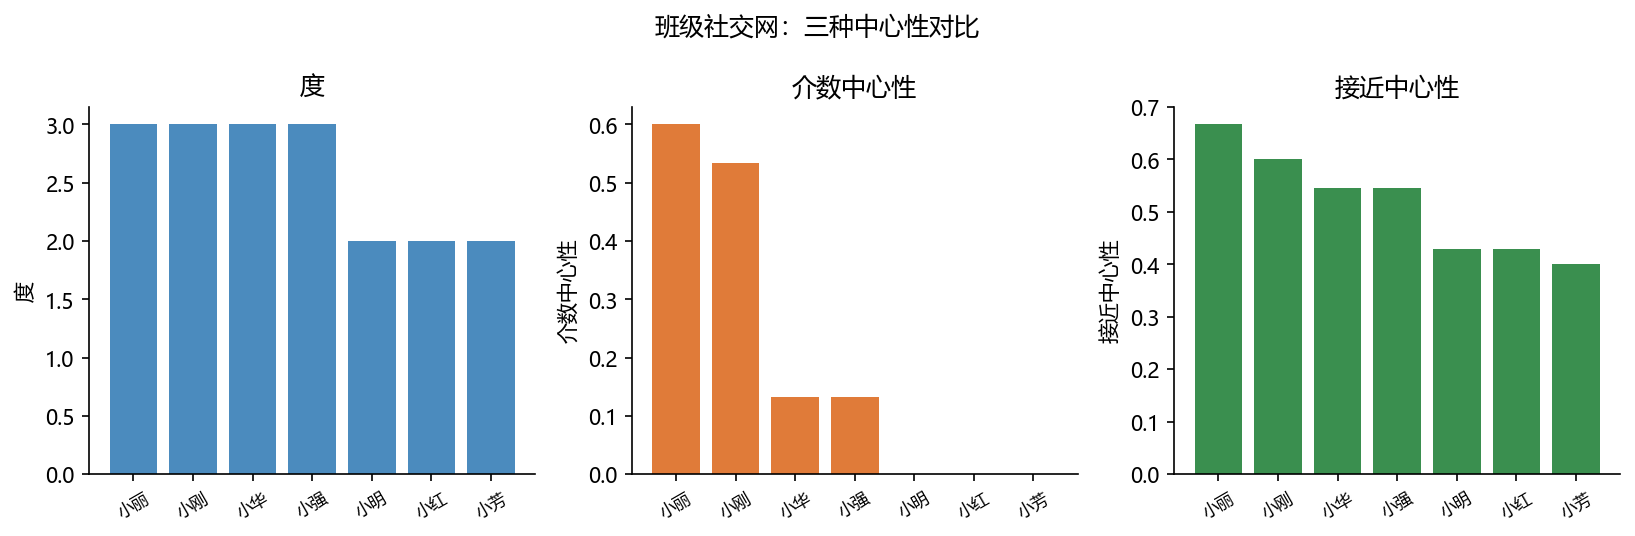
\includegraphics[keepaspectratio,alt={三种中心性对比}]{figures/06-networkx/case2_centrality.png}}
\caption{三种中心性对比}
\end{figure}

\subsubsection{主要用法 / API}\label{ux4e3bux8981ux7528ux6cd5-api-25}

{\def\LTcaptype{none} % do not increment counter
\begin{longtable}[]{@{}
  >{\raggedright\arraybackslash}p{(\linewidth - 4\tabcolsep) * \real{0.3333}}
  >{\raggedright\arraybackslash}p{(\linewidth - 4\tabcolsep) * \real{0.3333}}
  >{\raggedright\arraybackslash}p{(\linewidth - 4\tabcolsep) * \real{0.3333}}@{}}
\toprule\noalign{}
\begin{minipage}[b]{\linewidth}\raggedright
需求
\end{minipage} & \begin{minipage}[b]{\linewidth}\raggedright
写法
\end{minipage} & \begin{minipage}[b]{\linewidth}\raggedright
说明
\end{minipage} \\
\midrule\noalign{}
\endhead
\bottomrule\noalign{}
\endlastfoot
度中心性 & \texttt{nx.degree(G)} / \texttt{G.degree(node)} &
直接邻居数 \\
介数中心性 & \texttt{nx.betweenness\_centrality(G)} &
经过该点的最短路占比 \\
接近中心性 & \texttt{nx.closeness\_centrality(G)} &
平均距离越短越接近 \\
选最高 & \texttt{max(d,\ key=d.get)} 或
\texttt{sorted(d.items(),\ key=lambda\ x:\ (-x{[}1{]},\ x{[}0{]}))} &
找``最重要''节点 \\
批量画柱状图 & \texttt{plt.subplots(1,\ 3)} +
\texttt{ax.bar(names,\ vals)} & 三指标并排 \\
\end{longtable}
}

\subsubsection{常见错误}\label{ux5e38ux89c1ux9519ux8bef-25}

\begin{enumerate}
\def\labelenumi{\arabic{enumi}.}
\tightlist
\item
  以为``度最高=最重要''：本例度并列的有 4
  人，但真正扛起沟通的是介数最高的小丽。
\item
  直接 \texttt{print(nx.betweenness\_centrality(G))} 输出很多小数 →
  建议先 \texttt{round(v,\ 4)} 再打印。
\item
  用 \texttt{max(bc,\ key=bc.get)}
  只拿到``最高人''，但并列时只返回第一个；想要前三名要用
  \texttt{sorted(...){[}:3{]}}。
\item
  画条形图时不用 \texttt{sorted(C.nodes())} 固定顺序：如果直接用
  \texttt{C.nodes()} 的迭代顺序，不同环境可能顺序不同。
\end{enumerate}

\subsubsection{拓展 / 跟练}\label{ux62d3ux5c55-ux8ddfux7ec3-13}

\begin{enumerate}
\def\labelenumi{\arabic{enumi}.}
\tightlist
\item
  把小明和小芳直接连起来，观察小丽/小刚的介数如何下降。
\item
  在 \texttt{nx.karate\_club\_graph()} 上分别算三种中心性的前三名，比较
  0 号与 33 号谁更像``中心''。
\item
  用 \texttt{nx.betweenness\_centrality(G,\ k=20)} 在大图上做近似（k
  个随机源），并与精确值比较。
\item
  结合 \texttt{nx.community.greedy\_modularity\_communities}
  划分社区，再看``跨社区的桥节点''是不是就是介数最高的人。
\end{enumerate}

\begin{center}\rule{0.5\linewidth}{0.5pt}\end{center}

\subsection{常见误区}\label{ux5e38ux89c1ux8befux533a-18}

\begin{enumerate}
\def\labelenumi{\arabic{enumi}.}
\tightlist
\item
  \textbf{混淆度与中心性}：度只看``直接邻居数''，介数/接近中心性还考虑``经过该点的路径/到所有点的距离''，三者含义不同。
\item
  \textbf{在有向图上直接算
  average\_shortest\_path\_length}：默认需要图连通；若不连通，先取某个连通子图或用
  weak/strong 分量。
\item
  \textbf{把传递性当作``每个节点聚类系数的平均''}：两者定义不同（传递性按三角形/开放三元组分子分母算，平均聚类系数是各节点
  C 的均值）。
\item
  \textbf{社区划分结果不唯一}：贪心模块度算法对初始顺序、图结构敏感，Q
  只能说明``这个划分不错''，不等于``唯一正确答案''。
\item
  \textbf{计算介数中心性不限制节点数}：默认 exact
  精确算法在大图很慢；可用 k 参数抽样或只看部分节点。
\end{enumerate}

\subsection{思考题}\label{ux601dux8003ux9898-20}

\begin{enumerate}
\def\labelenumi{\arabic{enumi}.}
\tightlist
\item
  一个``星形图''（star\_graph(5)）的平均路径长度、直径、中心节点分别是什么？中心节点的介数中心性是多少？
\item
  为什么完全图（complete\_graph(10)）的平均聚类系数是 1，传递性也是 1？
\item
  给一个``连通但接近断裂''的图，哪个节点介数中心性最高？如何用代码找出``割点''？
\end{enumerate}

\subsection{动手练习（详见
lab）}\label{ux52a8ux624bux7ec3ux4e60ux8be6ux89c1-lab-12}

\begin{itemize}
\tightlist
\item
  构造
  path\_graph(8)，计算平均路径长度、直径、半径、各节点聚类系数与介数中心性；
\item
  构造两个连通分量，用 connected\_components 输出每个分量；
\item
  在 karate\_club\_graph 上分别计算 average\_clustering 与
  transitivity，比较并解释；
\item
  用 greedy\_modularity\_communities 划分 karate 网络，输出 Q
  与每个社区大小。
\end{itemize}

\subsection{延伸阅读}\label{ux5ef6ux4f38ux9605ux8bfb-27}

\begin{itemize}
\tightlist
\item
  NetworkX
  官方中心性算法：\href{https://networkx.org/documentation/stable/reference/algorithms/centrality.html}{链接}
\item
  NetworkX
  官方连通性算法：\href{https://networkx.org/documentation/stable/reference/algorithms/connectivity.html}{链接}
\item
  NetworkX
  官方社区检测：\href{https://networkx.org/documentation/stable/reference/algorithms/community.html}{链接}
\end{itemize}

\section{03
求解图的基本问题：遍历、最小生成树与最短路径}\label{ux6c42ux89e3ux56feux7684ux57faux672cux95eeux9898ux904dux5386ux6700ux5c0fux751fux6210ux6811ux4e0eux6700ux77edux8defux5f84}

\begin{quote}
本节对应原版 6.3
的内容。围绕三类经典问题：遍历（DFS/BFS）、最小生成树、最短路径。
\end{quote}

\subsection{本节目标}\label{ux672cux8282ux76eeux6807-25}

\begin{itemize}
\tightlist
\item
  会用 DFS / BFS 遍历图并得到节点访问顺序；
\item
  会用 minimum\_spanning\_tree 求解最小生成树并计算总权重；
\item
  会区分并使用 Dijkstra、Bellman-Ford、Floyd-Warshall 求解最短路径；
\item
  能根据图的特性（有权/无权、有负权/无负权、单源/全源）选择合适的算法。
\end{itemize}

\subsection{先修}\label{ux5148ux4fee-18}

\begin{itemize}
\tightlist
\item
  第 01 节：创建图、访问节点边；第 02 节：连通性概念。
\end{itemize}

\begin{center}\rule{0.5\linewidth}{0.5pt}\end{center}

\subsection{3.1 遍历问题（DFS /
BFS）}\label{ux904dux5386ux95eeux9898dfs-bfs}

\subsubsection{3.1.1
深度优先遍历（DFS）}\label{ux6df1ux5ea6ux4f18ux5148ux904dux5386dfs}

\begin{Shaded}
\begin{Highlighting}[]
\ImportTok{import}\NormalTok{ networkx }\ImportTok{as}\NormalTok{ nx}

\NormalTok{G }\OperatorTok{=}\NormalTok{ nx.Graph()}
\NormalTok{edges }\OperatorTok{=}\NormalTok{ [(}\DecValTok{1}\NormalTok{, }\DecValTok{2}\NormalTok{), (}\DecValTok{1}\NormalTok{, }\DecValTok{3}\NormalTok{), (}\DecValTok{2}\NormalTok{, }\DecValTok{4}\NormalTok{), (}\DecValTok{3}\NormalTok{, }\DecValTok{4}\NormalTok{), (}\DecValTok{4}\NormalTok{, }\DecValTok{5}\NormalTok{)]}
\NormalTok{G.add\_edges\_from(edges)}

\NormalTok{start\_node }\OperatorTok{=} \DecValTok{1}
\NormalTok{visited }\OperatorTok{=} \BuiltInTok{list}\NormalTok{(nx.dfs\_preorder\_nodes(G, start\_node))}
\BuiltInTok{print}\NormalTok{(}\StringTok{"DFS 遍历顺序:"}\NormalTok{, visited)}
\BuiltInTok{print}\NormalTok{(}\StringTok{"DFS 边:"}\NormalTok{, }\BuiltInTok{list}\NormalTok{(nx.dfs\_edges(G, start\_node)))}
\end{Highlighting}
\end{Shaded}

\begin{Shaded}
\begin{Highlighting}[]
\NormalTok{DFS 遍历顺序: [1, 2, 4, 3, 5]}
\NormalTok{DFS 边: [(1, 2), (2, 4), (4, 3), (4, 5)]}
\end{Highlighting}
\end{Shaded}

\subsubsection{3.1.2
广度优先遍历（BFS）}\label{ux5e7fux5ea6ux4f18ux5148ux904dux5386bfs}

bfs\_edges 返回按广度扩展的边，可由此构建节点访问顺序：

\begin{Shaded}
\begin{Highlighting}[]
\BuiltInTok{print}\NormalTok{(}\StringTok{"BFS 边:"}\NormalTok{, }\BuiltInTok{list}\NormalTok{(nx.bfs\_edges(G, start\_node)))}
\BuiltInTok{print}\NormalTok{(}\StringTok{"BFS 树边:"}\NormalTok{, }\BuiltInTok{list}\NormalTok{(nx.bfs\_tree(G, start\_node).edges()))}

\CommentTok{\#\# 用集合去重 + 列表保持顺序}
\NormalTok{seen }\OperatorTok{=} \BuiltInTok{set}\NormalTok{()}
\NormalTok{bfs\_order }\OperatorTok{=}\NormalTok{ []}
\ControlFlowTok{for}\NormalTok{ u, v }\KeywordTok{in}\NormalTok{ nx.bfs\_edges(G, start\_node):}
    \ControlFlowTok{if}\NormalTok{ u }\KeywordTok{not} \KeywordTok{in}\NormalTok{ seen:}
\NormalTok{        seen.add(u)}\OperatorTok{;}\NormalTok{ bfs\_order.append(u)}
    \ControlFlowTok{if}\NormalTok{ v }\KeywordTok{not} \KeywordTok{in}\NormalTok{ seen:}
\NormalTok{        seen.add(v)}\OperatorTok{;}\NormalTok{ bfs\_order.append(v)}
\BuiltInTok{print}\NormalTok{(}\StringTok{"BFS 节点顺序:"}\NormalTok{, bfs\_order)}
\end{Highlighting}
\end{Shaded}

\begin{Shaded}
\begin{Highlighting}[]
\NormalTok{BFS 边: [(1, 2), (1, 3), (2, 4), (4, 5)]}
\NormalTok{BFS 树边: [(1, 2), (1, 3), (2, 4), (4, 5)]}
\NormalTok{BFS 节点顺序: [1, 2, 3, 4, 5]}
\end{Highlighting}
\end{Shaded}

\begin{quote}
DFS 优先``一条路走到黑''，BFS 按``层''逐层扩散。在无权图上，BFS
得到的路径就是最短路径（边数最少）。
\end{quote}

\begin{center}\rule{0.5\linewidth}{0.5pt}\end{center}

\subsection{3.2 最小生成树（Minimum Spanning Tree,
MST）}\label{ux6700ux5c0fux751fux6210ux6811minimum-spanning-tree-mst}

\subsubsection{3.2.1 问题}\label{ux95eeux9898}

给定一个加权无向连通图，找到一棵边的总权重最小的生成树（连接所有节点且无环）。NetworkX
提供 minimum\_spanning\_tree，默认用 Kruskal
算法（适合稀疏图）；稠密图可考虑 Prim 思想，但官方没有直接的 Prim
选项，多数场景 Kruskal 已足够。

\begin{Shaded}
\begin{Highlighting}[]
\NormalTok{G }\OperatorTok{=}\NormalTok{ nx.Graph()}
\NormalTok{edges }\OperatorTok{=}\NormalTok{ [}
\NormalTok{    (}\StringTok{"A"}\NormalTok{, }\StringTok{"B"}\NormalTok{, }\DecValTok{10}\NormalTok{),}
\NormalTok{    (}\StringTok{"A"}\NormalTok{, }\StringTok{"C"}\NormalTok{, }\DecValTok{6}\NormalTok{),}
\NormalTok{    (}\StringTok{"A"}\NormalTok{, }\StringTok{"D"}\NormalTok{, }\DecValTok{5}\NormalTok{),}
\NormalTok{    (}\StringTok{"B"}\NormalTok{, }\StringTok{"C"}\NormalTok{, }\DecValTok{5}\NormalTok{),}
\NormalTok{    (}\StringTok{"B"}\NormalTok{, }\StringTok{"D"}\NormalTok{, }\DecValTok{15}\NormalTok{),}
\NormalTok{    (}\StringTok{"B"}\NormalTok{, }\StringTok{"E"}\NormalTok{, }\DecValTok{4}\NormalTok{),}
\NormalTok{    (}\StringTok{"C"}\NormalTok{, }\StringTok{"D"}\NormalTok{, }\DecValTok{15}\NormalTok{),}
\NormalTok{    (}\StringTok{"C"}\NormalTok{, }\StringTok{"F"}\NormalTok{, }\DecValTok{12}\NormalTok{),}
\NormalTok{    (}\StringTok{"D"}\NormalTok{, }\StringTok{"E"}\NormalTok{, }\DecValTok{20}\NormalTok{),}
\NormalTok{    (}\StringTok{"E"}\NormalTok{, }\StringTok{"F"}\NormalTok{, }\DecValTok{9}\NormalTok{),}
\NormalTok{]}
\NormalTok{G.add\_weighted\_edges\_from(edges)}

\NormalTok{T }\OperatorTok{=}\NormalTok{ nx.minimum\_spanning\_tree(G)}

\BuiltInTok{print}\NormalTok{(}\StringTok{"MST 边："}\NormalTok{)}
\ControlFlowTok{for}\NormalTok{ u, v, weight }\KeywordTok{in}\NormalTok{ T.edges(data}\OperatorTok{=}\StringTok{"weight"}\NormalTok{):}
    \BuiltInTok{print}\NormalTok{(u, }\StringTok{"{-}{-}"}\NormalTok{, v, }\StringTok{"weighted"}\NormalTok{, weight)}
\BuiltInTok{print}\NormalTok{(}\StringTok{"MST 总权重:"}\NormalTok{, }\BuiltInTok{sum}\NormalTok{(w }\ControlFlowTok{for}\NormalTok{ \_, \_, w }\KeywordTok{in}\NormalTok{ T.edges(data}\OperatorTok{=}\StringTok{"weight"}\NormalTok{)))}
\BuiltInTok{print}\NormalTok{(}\StringTok{"MST 边数:"}\NormalTok{, T.number\_of\_edges())}
\end{Highlighting}
\end{Shaded}

\begin{Shaded}
\begin{Highlighting}[]
\NormalTok{MST 边：}
\NormalTok{A {-}{-} D weighted 5}
\NormalTok{A {-}{-} C weighted 6}
\NormalTok{B {-}{-} E weighted 4}
\NormalTok{B {-}{-} C weighted 5}
\NormalTok{E {-}{-} F weighted 9}
\NormalTok{MST 总权重: 29}
\NormalTok{MST 边数: 5}
\end{Highlighting}
\end{Shaded}

\begin{quote}
选择边 \{B-E(4), A-D(5), B-C(5), A-C(6), E-F(9)\}，总权重 29；连通
A、B、C、D、E、F 且无环。
\end{quote}

\begin{center}\rule{0.5\linewidth}{0.5pt}\end{center}

\subsection{3.3
最短路径问题}\label{ux6700ux77edux8defux5f84ux95eeux9898}

\subsubsection{3.3.1 Dijkstra
算法（非负权、单源）}\label{dijkstra-ux7b97ux6cd5ux975eux8d1fux6743ux5355ux6e90}

适用于边权非负的图。用 dijkstra\_path 求路径，dijkstra\_path\_length
求长度。

\begin{Shaded}
\begin{Highlighting}[]
\NormalTok{DG }\OperatorTok{=}\NormalTok{ nx.DiGraph()}
\NormalTok{DG.add\_edge(}\StringTok{"A"}\NormalTok{, }\StringTok{"B"}\NormalTok{, weight}\OperatorTok{=}\DecValTok{3}\NormalTok{)}
\NormalTok{DG.add\_edge(}\StringTok{"A"}\NormalTok{, }\StringTok{"C"}\NormalTok{, weight}\OperatorTok{=}\DecValTok{2}\NormalTok{)}
\NormalTok{DG.add\_edge(}\StringTok{"B"}\NormalTok{, }\StringTok{"C"}\NormalTok{, weight}\OperatorTok{=}\DecValTok{1}\NormalTok{)}
\NormalTok{DG.add\_edge(}\StringTok{"B"}\NormalTok{, }\StringTok{"D"}\NormalTok{, weight}\OperatorTok{=}\DecValTok{4}\NormalTok{)}
\NormalTok{DG.add\_edge(}\StringTok{"C"}\NormalTok{, }\StringTok{"D"}\NormalTok{, weight}\OperatorTok{=}\DecValTok{2}\NormalTok{)}
\NormalTok{DG.add\_edge(}\StringTok{"C"}\NormalTok{, }\StringTok{"E"}\NormalTok{, weight}\OperatorTok{=}\DecValTok{1}\NormalTok{)}
\NormalTok{DG.add\_edge(}\StringTok{"D"}\NormalTok{, }\StringTok{"E"}\NormalTok{, weight}\OperatorTok{=}\DecValTok{3}\NormalTok{)}

\NormalTok{shortest\_path }\OperatorTok{=}\NormalTok{ nx.dijkstra\_path(DG, }\StringTok{"A"}\NormalTok{, }\StringTok{"E"}\NormalTok{, weight}\OperatorTok{=}\StringTok{"weight"}\NormalTok{)}
\NormalTok{shortest\_length }\OperatorTok{=}\NormalTok{ nx.dijkstra\_path\_length(DG, }\StringTok{"A"}\NormalTok{, }\StringTok{"E"}\NormalTok{, weight}\OperatorTok{=}\StringTok{"weight"}\NormalTok{)}
\BuiltInTok{print}\NormalTok{(}\StringTok{"最短路径:"}\NormalTok{, shortest\_path)}
\BuiltInTok{print}\NormalTok{(}\StringTok{"最短路径长度:"}\NormalTok{, shortest\_length)}

\CommentTok{\#\# 从 A 到所有点的最短距离}
\BuiltInTok{print}\NormalTok{(}\StringTok{"单源最短路径长度:"}\NormalTok{, nx.single\_source\_dijkstra\_path\_length(DG, }\StringTok{"A"}\NormalTok{, weight}\OperatorTok{=}\StringTok{"weight"}\NormalTok{))}
\end{Highlighting}
\end{Shaded}

\begin{Shaded}
\begin{Highlighting}[]
\NormalTok{最短路径: [\textquotesingle{}A\textquotesingle{}, \textquotesingle{}C\textquotesingle{}, \textquotesingle{}E\textquotesingle{}]}
\NormalTok{最短路径长度: 3}
\NormalTok{单源最短路径长度: \{\textquotesingle{}A\textquotesingle{}: 0, \textquotesingle{}C\textquotesingle{}: 2, \textquotesingle{}B\textquotesingle{}: 3, \textquotesingle{}E\textquotesingle{}: 3, \textquotesingle{}D\textquotesingle{}: 4\}}
\end{Highlighting}
\end{Shaded}

注意：从 A 到 E 走 A→C→E 是 2+1=3，比 A→B→C→E（3+1+1=5）和
A→C→D→E（2+2+3=7）都短。

\subsubsection{3.3.2 Bellman-Ford
算法（可处理负权边、单源）}\label{bellman-ford-ux7b97ux6cd5ux53efux5904ux7406ux8d1fux6743ux8fb9ux5355ux6e90}

当图中存在负权边（但没有负权回路）时，Dijkstra 不再适用，可用
Bellman-Ford。时间复杂度 O(VE)。

\begin{Shaded}
\begin{Highlighting}[]
\BuiltInTok{print}\NormalTok{(}\StringTok{"Bellman{-}Ford 路径:"}\NormalTok{, nx.bellman\_ford\_path(DG, }\StringTok{"A"}\NormalTok{, }\StringTok{"E"}\NormalTok{, weight}\OperatorTok{=}\StringTok{"weight"}\NormalTok{))}
\BuiltInTok{print}\NormalTok{(}\StringTok{"Bellman{-}Ford 长度:"}\NormalTok{, nx.bellman\_ford\_path\_length(DG, }\StringTok{"A"}\NormalTok{, }\StringTok{"E"}\NormalTok{, weight}\OperatorTok{=}\StringTok{"weight"}\NormalTok{))}
\end{Highlighting}
\end{Shaded}

\begin{Shaded}
\begin{Highlighting}[]
\NormalTok{Bellman{-}Ford 路径: [\textquotesingle{}A\textquotesingle{}, \textquotesingle{}C\textquotesingle{}, \textquotesingle{}E\textquotesingle{}]}
\NormalTok{Bellman{-}Ford 长度: 3}
\end{Highlighting}
\end{Shaded}

\subsubsection{3.3.3 Floyd-Warshall
算法（全源最短路径）}\label{floyd-warshall-ux7b97ux6cd5ux5168ux6e90ux6700ux77edux8defux5f84}

需要``所有点对之间的最短距离''时用 Floyd-Warshall，O(V\^{}3)。networkx
提供 floyd\_warshall / floyd\_warshall\_numpy。

\begin{Shaded}
\begin{Highlighting}[]
\ImportTok{import}\NormalTok{ numpy }\ImportTok{as}\NormalTok{ np}
\NormalTok{path\_lengths }\OperatorTok{=}\NormalTok{ nx.floyd\_warshall\_numpy(DG, weight}\OperatorTok{=}\StringTok{"weight"}\NormalTok{)}
\BuiltInTok{print}\NormalTok{(}\StringTok{"矩阵形状:"}\NormalTok{, path\_lengths.shape)}
\NormalTok{idx }\OperatorTok{=} \BuiltInTok{list}\NormalTok{(DG.nodes())}
\NormalTok{iA }\OperatorTok{=}\NormalTok{ idx.index(}\StringTok{"A"}\NormalTok{)}\OperatorTok{;}\NormalTok{ iE }\OperatorTok{=}\NormalTok{ idx.index(}\StringTok{"E"}\NormalTok{)}
\BuiltInTok{print}\NormalTok{(}\StringTok{"A 到 E 的距离:"}\NormalTok{, path\_lengths[iA, iE])}
\BuiltInTok{print}\NormalTok{(}\StringTok{"A 行:"}\NormalTok{, path\_lengths[iA, :])}
\end{Highlighting}
\end{Shaded}

\begin{Shaded}
\begin{Highlighting}[]
\NormalTok{矩阵形状: (5, 5)}
\NormalTok{A 到 E 的距离: 3.0}
\NormalTok{A 行: [0. 3. 2. 4. 3.]}
\end{Highlighting}
\end{Shaded}

\begin{quote}
Floyd-Warshall 不直接返回路径；若需要路径，可结合 shortest\_path
逐步重建，或用 nx.shortest\_path(G, source, target, weight=``weight'')
得到一条具体路径。
\end{quote}

\subsubsection{3.3.4
算法选择速查}\label{ux7b97ux6cd5ux9009ux62e9ux901fux67e5}

{\def\LTcaptype{none} % do not increment counter
\begin{longtable}[]{@{}
  >{\raggedright\arraybackslash}p{(\linewidth - 6\tabcolsep) * \real{0.2500}}
  >{\raggedright\arraybackslash}p{(\linewidth - 6\tabcolsep) * \real{0.2500}}
  >{\raggedright\arraybackslash}p{(\linewidth - 6\tabcolsep) * \real{0.2500}}
  >{\raggedright\arraybackslash}p{(\linewidth - 6\tabcolsep) * \real{0.2500}}@{}}
\toprule\noalign{}
\begin{minipage}[b]{\linewidth}\raggedright
需求
\end{minipage} & \begin{minipage}[b]{\linewidth}\raggedright
图特性
\end{minipage} & \begin{minipage}[b]{\linewidth}\raggedright
推荐函数
\end{minipage} & \begin{minipage}[b]{\linewidth}\raggedright
复杂度
\end{minipage} \\
\midrule\noalign{}
\endhead
\bottomrule\noalign{}
\endlastfoot
单源、非负权 & 无负权 & dijkstra\_path / dijkstra\_path\_length &
O((V+E) log V) \\
单源、可能有负权 & 允许负权但无负环 & bellman\_ford\_path & O(VE) \\
全源最短距离 & 可含负权（无负环） & floyd\_warshall /
floyd\_warshall\_numpy & O(V\^{}3) \\
无权最短路径 & 边权都为 1 & shortest\_path / bfs & O(V+E) \\
\end{longtable}
}

\subsection{案例卡
3：加权最短路径------地铁换乘总时间最少路线}\label{ux6848ux4f8bux5361-3ux52a0ux6743ux6700ux77edux8defux5f84ux5730ux94c1ux6362ux4e58ux603bux65f6ux95f4ux6700ux5c11ux8defux7ebf}

\subsubsection{目标}\label{ux76eeux6807-26}

把地铁站当节点、站间行驶时间(分钟)当\textbf{边权}，用
\texttt{nx.dijkstra\_path}
求``从中央公园到科技园''总时间最少的换乘路线，并打印从起点到所有站的最少时间。这是``带权图上找最短路''的典型应用。

\subsubsection{代码}\label{ux4ee3ux7801-27}

\begin{Shaded}
\begin{Highlighting}[]
\ImportTok{import}\NormalTok{ networkx }\ImportTok{as}\NormalTok{ nx}
\ImportTok{import}\NormalTok{ matplotlib.pyplot }\ImportTok{as}\NormalTok{ plt}
\ImportTok{import}\NormalTok{ numpy }\ImportTok{as}\NormalTok{ np}
\ImportTok{import}\NormalTok{ os}

\NormalTok{plt.rcParams[}\StringTok{\textquotesingle{}font.sans{-}serif\textquotesingle{}}\NormalTok{] }\OperatorTok{=}\NormalTok{ [}\StringTok{\textquotesingle{}Microsoft YaHei\textquotesingle{}}\NormalTok{, }\StringTok{\textquotesingle{}SimHei\textquotesingle{}}\NormalTok{, }\StringTok{\textquotesingle{}DejaVu Sans\textquotesingle{}}\NormalTok{]}
\NormalTok{plt.rcParams[}\StringTok{\textquotesingle{}axes.unicode\_minus\textquotesingle{}}\NormalTok{] }\OperatorTok{=} \VariableTok{False}
\NormalTok{np.set\_printoptions(precision}\OperatorTok{=}\DecValTok{4}\NormalTok{, suppress}\OperatorTok{=}\VariableTok{True}\NormalTok{)}

\CommentTok{\#\# 1) 地铁网：节点=车站，边的 weight=行驶分钟(双向)}
\NormalTok{M }\OperatorTok{=}\NormalTok{ nx.Graph()}
\NormalTok{M.add\_weighted\_edges\_from([}
\NormalTok{    (}\StringTok{\textquotesingle{}中央公园\textquotesingle{}}\NormalTok{,}\StringTok{\textquotesingle{}城东\textquotesingle{}}\NormalTok{, }\DecValTok{3}\NormalTok{), (}\StringTok{\textquotesingle{}中央公园\textquotesingle{}}\NormalTok{,}\StringTok{\textquotesingle{}大学城\textquotesingle{}}\NormalTok{, }\DecValTok{2}\NormalTok{),}
\NormalTok{    (}\StringTok{\textquotesingle{}城东\textquotesingle{}}\NormalTok{,}\StringTok{\textquotesingle{}大学城\textquotesingle{}}\NormalTok{, }\DecValTok{1}\NormalTok{), (}\StringTok{\textquotesingle{}城东\textquotesingle{}}\NormalTok{,}\StringTok{\textquotesingle{}火车站\textquotesingle{}}\NormalTok{, }\DecValTok{4}\NormalTok{), (}\StringTok{\textquotesingle{}大学城\textquotesingle{}}\NormalTok{,}\StringTok{\textquotesingle{}火车站\textquotesingle{}}\NormalTok{, }\DecValTok{2}\NormalTok{),}
\NormalTok{    (}\StringTok{\textquotesingle{}大学城\textquotesingle{}}\NormalTok{,}\StringTok{\textquotesingle{}机场\textquotesingle{}}\NormalTok{, }\DecValTok{1}\NormalTok{), (}\StringTok{\textquotesingle{}火车站\textquotesingle{}}\NormalTok{,}\StringTok{\textquotesingle{}机场\textquotesingle{}}\NormalTok{, }\DecValTok{3}\NormalTok{), (}\StringTok{\textquotesingle{}火车站\textquotesingle{}}\NormalTok{,}\StringTok{\textquotesingle{}科技园\textquotesingle{}}\NormalTok{, }\DecValTok{2}\NormalTok{), (}\StringTok{\textquotesingle{}机场\textquotesingle{}}\NormalTok{,}\StringTok{\textquotesingle{}科技园\textquotesingle{}}\NormalTok{, }\DecValTok{4}\NormalTok{),}
\NormalTok{])}

\CommentTok{\#\# 2) Dijkstra：单源最短路径/长度(默认按边权)}
\NormalTok{path }\OperatorTok{=}\NormalTok{ nx.dijkstra\_path(M, }\StringTok{\textquotesingle{}中央公园\textquotesingle{}}\NormalTok{, }\StringTok{\textquotesingle{}科技园\textquotesingle{}}\NormalTok{, weight}\OperatorTok{=}\StringTok{\textquotesingle{}weight\textquotesingle{}}\NormalTok{)}
\NormalTok{length }\OperatorTok{=}\NormalTok{ nx.dijkstra\_path\_length(M, }\StringTok{\textquotesingle{}中央公园\textquotesingle{}}\NormalTok{, }\StringTok{\textquotesingle{}科技园\textquotesingle{}}\NormalTok{, weight}\OperatorTok{=}\StringTok{\textquotesingle{}weight\textquotesingle{}}\NormalTok{)}
\BuiltInTok{print}\NormalTok{(}\StringTok{\textquotesingle{}最短路径:\textquotesingle{}}\NormalTok{, path)}
\BuiltInTok{print}\NormalTok{(}\StringTok{\textquotesingle{}最短时间(分钟):\textquotesingle{}}\NormalTok{, length)}

\CommentTok{\#\# 3) 从起点到所有站的最少时间(按站名排序保证顺序稳定)}
\NormalTok{sdd }\OperatorTok{=}\NormalTok{ nx.single\_source\_dijkstra\_path\_length(M, }\StringTok{\textquotesingle{}中央公园\textquotesingle{}}\NormalTok{, weight}\OperatorTok{=}\StringTok{\textquotesingle{}weight\textquotesingle{}}\NormalTok{)}
\BuiltInTok{print}\NormalTok{(}\StringTok{\textquotesingle{}单源最短时间(按站名排序):\textquotesingle{}}\NormalTok{, \{k: }\BuiltInTok{round}\NormalTok{(v, }\DecValTok{4}\NormalTok{) }\ControlFlowTok{for}\NormalTok{ k, v }\KeywordTok{in} \BuiltInTok{sorted}\NormalTok{(sdd.items())\})}

\CommentTok{\#\# 4) 把最短路线画出来}
\NormalTok{path\_edges }\OperatorTok{=} \BuiltInTok{list}\NormalTok{(}\BuiltInTok{zip}\NormalTok{(path[:}\OperatorTok{{-}}\DecValTok{1}\NormalTok{], path[}\DecValTok{1}\NormalTok{:]))}
\NormalTok{pos }\OperatorTok{=}\NormalTok{ nx.spring\_layout(M, seed}\OperatorTok{=}\DecValTok{42}\NormalTok{, k}\OperatorTok{=}\FloatTok{0.9}\NormalTok{)}
\NormalTok{os.makedirs(}\StringTok{\textquotesingle{}images\textquotesingle{}}\NormalTok{, exist\_ok}\OperatorTok{=}\VariableTok{True}\NormalTok{)}
\NormalTok{plt.figure(figsize}\OperatorTok{=}\NormalTok{(}\FloatTok{7.0}\NormalTok{, }\FloatTok{5.0}\NormalTok{))}
\NormalTok{nx.draw\_networkx\_nodes(M, pos, node\_size}\OperatorTok{=}\DecValTok{650}\NormalTok{, node\_color}\OperatorTok{=}\StringTok{\textquotesingle{}\#dff3e0\textquotesingle{}}\NormalTok{, edgecolors}\OperatorTok{=}\StringTok{\textquotesingle{}\#3a8f4f\textquotesingle{}}\NormalTok{)}
\NormalTok{nx.draw\_networkx\_edges(M, pos, alpha}\OperatorTok{=}\FloatTok{0.35}\NormalTok{, edge\_color}\OperatorTok{=}\StringTok{\textquotesingle{}\#999999\textquotesingle{}}\NormalTok{, width}\OperatorTok{=}\FloatTok{1.2}\NormalTok{)}
\NormalTok{nx.draw\_networkx\_edges(M, pos, edgelist}\OperatorTok{=}\NormalTok{path\_edges, edge\_color}\OperatorTok{=}\StringTok{\textquotesingle{}\#c0392b\textquotesingle{}}\NormalTok{, width}\OperatorTok{=}\FloatTok{3.0}\NormalTok{)}
\NormalTok{nx.draw\_networkx\_labels(M, pos, font\_size}\OperatorTok{=}\DecValTok{11}\NormalTok{, font\_family}\OperatorTok{=}\StringTok{\textquotesingle{}Microsoft YaHei\textquotesingle{}}\NormalTok{)}
\NormalTok{plt.title(}\StringTok{\textquotesingle{}地铁网：中央公园 {-}\textgreater{} 科技园 最少时间路线\textquotesingle{}}\NormalTok{)}
\NormalTok{plt.axis(}\StringTok{\textquotesingle{}off\textquotesingle{}}\NormalTok{)}
\NormalTok{plt.tight\_layout()}
\NormalTok{plt.savefig(}\StringTok{\textquotesingle{}figures/06{-}networkx/case3\_metro.png\textquotesingle{}}\NormalTok{, dpi}\OperatorTok{=}\DecValTok{150}\NormalTok{)}
\BuiltInTok{print}\NormalTok{(}\StringTok{\textquotesingle{}已保存 figures/06{-}networkx/case3\_metro.png\textquotesingle{}}\NormalTok{)}
\NormalTok{plt.close()}
\end{Highlighting}
\end{Shaded}

\subsubsection{运行结果(已运行核验)}\label{ux8fd0ux884cux7ed3ux679cux5df2ux8fd0ux884cux6838ux9a8c-25}

\begin{Shaded}
\begin{Highlighting}[]
\NormalTok{最短路径: [\textquotesingle{}中央公园\textquotesingle{}, \textquotesingle{}大学城\textquotesingle{}, \textquotesingle{}火车站\textquotesingle{}, \textquotesingle{}科技园\textquotesingle{}]}
\NormalTok{最短时间(分钟): 6}
\NormalTok{单源最短时间(按站名排序): \{\textquotesingle{}中央公园\textquotesingle{}: 0, \textquotesingle{}城东\textquotesingle{}: 3, \textquotesingle{}大学城\textquotesingle{}: 2, \textquotesingle{}机场\textquotesingle{}: 3, \textquotesingle{}火车站\textquotesingle{}: 4, \textquotesingle{}科技园\textquotesingle{}: 6\}}
\NormalTok{已保存 figures/06{-}networkx/case3\_metro.png}
\end{Highlighting}
\end{Shaded}

\subsubsection{讲解}\label{ux8bb2ux89e3-25}

\textbf{一句话解释}：每条地铁线都标上``坐多久''，Dijkstra
就会像贪心一样从起点出发，每次先挑``目前累计时间最少''的站往前扩，最后得到总时间最少的换乘方案。

\begin{enumerate}
\def\labelenumi{\arabic{enumi}.}
\tightlist
\item
  \texttt{M.add\_weighted\_edges\_from(...)} 每条边的 \texttt{weight}
  就是行驶分钟；地铁双向能坐，所以用无向 \texttt{nx.Graph} 即可。
\item
  \texttt{nx.dijkstra\_path(M,\ \textquotesingle{}中央公园\textquotesingle{},\ \textquotesingle{}科技园\textquotesingle{},\ weight=\textquotesingle{}weight\textquotesingle{})}
  返回\textbf{一条}路径
  \texttt{{[}\textquotesingle{}中央公园\textquotesingle{},\textquotesingle{}大学城\textquotesingle{},\textquotesingle{}火车站\textquotesingle{},\textquotesingle{}科技园\textquotesingle{}{]}}，时间是
  2+2+2=6 分钟。
\item
  \texttt{nx.dijkstra\_path\_length(...)} 只返回总时间
  6；\texttt{nx.single\_source\_dijkstra\_path\_length(...)}
  返回从起点到\textbf{每个站}的最少时间，例如到机场 3 分钟（经大学城
  2+1），到火车站 4 分钟（经大学城 2+2）。
\item
  注意 \texttt{weight=\textquotesingle{}weight\textquotesingle{}}
  不能漏：如果不传，NetworkX 默认把所有边权当成
  1，那就变成``换乘站数最少''，结果会不一样。
\item
  为什么走``中央公园→大学城→火车站→科技园''而不是``机场→科技园''那条？因为机场-科技园要
  4 分钟，而大学城-机场只要 1+3=4 分钟，两者到科技园都 4
  分钟；但走大学城-火车站-科技园是 2+2=4 分钟，所以整体最短是 6 分钟。
\item
  绘图用 \texttt{spring\_layout(...,\ seed=42)}
  固定布局，红色高亮最短路径；\texttt{os.makedirs(\textquotesingle{}images\textquotesingle{},\ exist\_ok=True)}
  保证目录存在。
\end{enumerate}

\begin{figure}
\centering
\pandocbounded{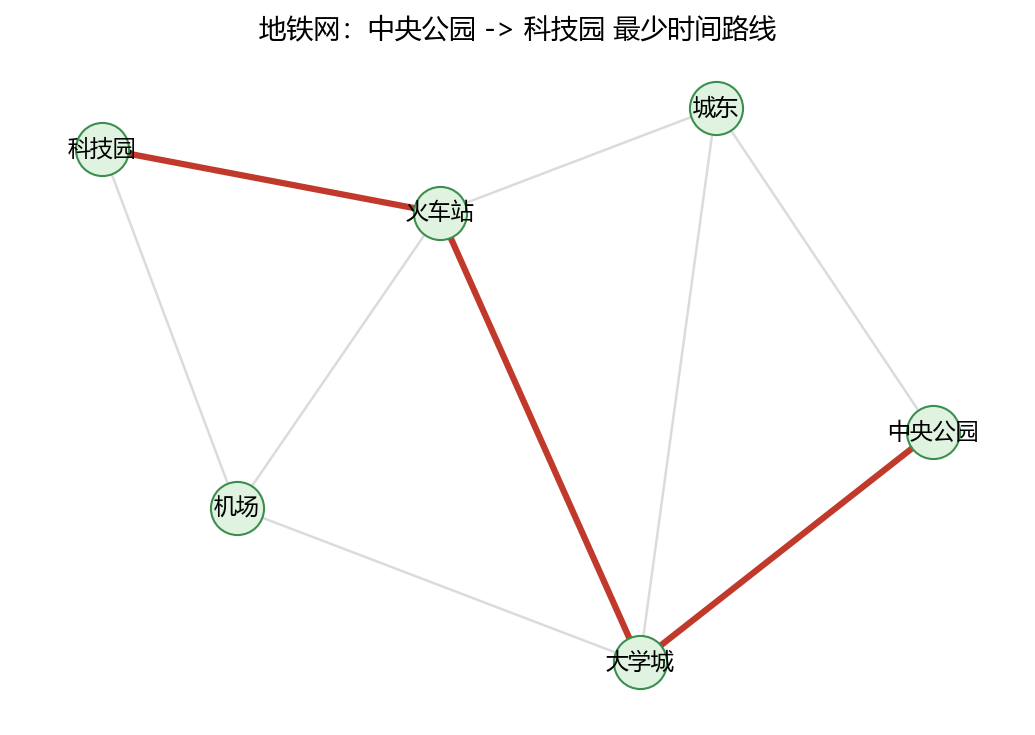
\includegraphics[keepaspectratio,alt={地铁最少时间路线}]{figures/06-networkx/case3_metro.png}}
\caption{地铁最少时间路线}
\end{figure}

\subsubsection{主要用法 / API}\label{ux4e3bux8981ux7528ux6cd5-api-26}

{\def\LTcaptype{none} % do not increment counter
\begin{longtable}[]{@{}
  >{\raggedright\arraybackslash}p{(\linewidth - 4\tabcolsep) * \real{0.3333}}
  >{\raggedright\arraybackslash}p{(\linewidth - 4\tabcolsep) * \real{0.3333}}
  >{\raggedright\arraybackslash}p{(\linewidth - 4\tabcolsep) * \real{0.3333}}@{}}
\toprule\noalign{}
\begin{minipage}[b]{\linewidth}\raggedright
需求
\end{minipage} & \begin{minipage}[b]{\linewidth}\raggedright
写法
\end{minipage} & \begin{minipage}[b]{\linewidth}\raggedright
说明
\end{minipage} \\
\midrule\noalign{}
\endhead
\bottomrule\noalign{}
\endlastfoot
加带权边 & \texttt{add\_weighted\_edges\_from({[}(u,\ v,\ w){]})} &
属性名 \texttt{weight} \\
单源最短路 &
\texttt{nx.dijkstra\_path(G,\ s,\ t,\ weight=\textquotesingle{}weight\textquotesingle{})}
& 返回一条路径 \\
最短距离 &
\texttt{nx.dijkstra\_path\_length(G,\ s,\ t,\ weight=\textquotesingle{}weight\textquotesingle{})}
& 返回总权重 \\
到所有点距离 &
\texttt{nx.single\_source\_dijkstra\_path\_length(G,\ s,\ weight=\textquotesingle{}weight\textquotesingle{})}
& 返回 dict \\
全源距离矩阵 &
\texttt{nx.floyd\_warshall\_numpy(G,\ weight=\textquotesingle{}weight\textquotesingle{})}
& 任意两点距离 \\
有负权边 &
\texttt{nx.bellman\_ford\_path(G,\ s,\ t,\ weight=\textquotesingle{}weight\textquotesingle{})}
& 改用 Bellman-Ford \\
\end{longtable}
}

\subsubsection{常见错误}\label{ux5e38ux89c1ux9519ux8bef-26}

\begin{enumerate}
\def\labelenumi{\arabic{enumi}.}
\tightlist
\item
  忘了
  \texttt{weight=\textquotesingle{}weight\textquotesingle{}}：带权图会被当成无权图，结果变成``换乘/站数最少''而不是``时间最少''。
\item
  在含负权边的图上用 Dijkstra：Dijkstra
  假设非负权；有负权（无负环）时应改用 \texttt{bellman\_ford\_path} 或
  \texttt{floyd\_warshall}。
\item
  \texttt{single\_source\_dijkstra\_path\_length} 返回的 dict 顺序不确定
  → 打印前用 \texttt{sorted(d.items())} 固定。
\item
  以为``总时间最少''等价于``经过站最少''：本例最短时间路线是 4 站 3
  段；但若把机场-科技园改成 1 分钟，最短时间路线就变成经机场的 3
  段，与少换乘目标不同。
\end{enumerate}

\subsubsection{拓展 / 跟练}\label{ux62d3ux5c55-ux8ddfux7ec3-14}

\begin{enumerate}
\def\labelenumi{\arabic{enumi}.}
\tightlist
\item
  新增一条``机场-城东''直达线(2
  分钟)，重新计算最短路与最短时间，看是否变短。
\item
  用
  \texttt{nx.shortest\_path(M,\ \textquotesingle{}中央公园\textquotesingle{},\ \textquotesingle{}科技园\textquotesingle{})}(不带
  weight)对比``站数最少''与``时间最少''两条路线。
\item
  把权重视为``票价''，用 \texttt{nx.bellman\_ford\_path}
  重算（本例无负权，结果应一致）。
\item
  用
  \texttt{nx.floyd\_warshall\_numpy(M,\ weight=\textquotesingle{}weight\textquotesingle{})}
  输出 6x6 距离矩阵，并验证对角元为 0。
\end{enumerate}

\begin{center}\rule{0.5\linewidth}{0.5pt}\end{center}

\subsection{常见误区}\label{ux5e38ux89c1ux8befux533a-19}

\begin{enumerate}
\def\labelenumi{\arabic{enumi}.}
\tightlist
\item
  \textbf{在无权图上用 Dijkstra 还传 weight=``weight''}：无权图没有
  weight 属性，直接用 shortest\_path / bfs 即可，或明确传 weight=None。
\item
  \textbf{在有负权边的图上用 Dijkstra}：Dijkstra
  假设非负权，负权会给出错误结果，应改用 Bellman-Ford。
\item
  \textbf{对不连通图调用 diameter /
  average\_shortest\_path\_length}：会抛错，先检查连通性或用连通分量分别计算。
\item
  \textbf{把 minimum\_spanning\_tree 的边权当成``路径权重''}：MST
  是为了连通所有节点总权重最小，与最短路径目标不同；两者不能混用。
\item
  \textbf{忘记 graph 需要连通才能有 MST}：minimum\_spanning\_tree
  要求输入连通（或每个分量各自生成森林）。
\end{enumerate}

\subsection{思考题}\label{ux601dux8003ux9898-21}

\begin{enumerate}
\def\labelenumi{\arabic{enumi}.}
\tightlist
\item
  BFS 在无权图上求出的路径是最短的吗？为什么？
\item
  最小生成树与最短路径有何区别？一个是``连所有点''，一个是``两点之间距离''。
\item
  对于含负权边的有向图，Floyd-Warshall
  能否给出正确答案？什么情况下会失败？
\end{enumerate}

\subsection{动手练习（详见
lab）}\label{ux52a8ux624bux7ec3ux4e60ux8be6ux89c1-lab-13}

\begin{itemize}
\tightlist
\item
  构造 path\_graph(8)，从节点 0 出发分别用 DFS、BFS 输出顺序，比较差异；
\item
  构造上面的加权图，用 minimum\_spanning\_tree 求 MST，并验证总权重=29；
\item
  构造带负权边的图，比较 Dijkstra 与 Bellman-Ford 的结果差异；
\item
  用 floyd\_warshall\_numpy 计算两两距离矩阵，并验证对角元为 0。
\end{itemize}

\subsection{延伸阅读}\label{ux5ef6ux4f38ux9605ux8bfb-28}

\begin{itemize}
\tightlist
\item
  NetworkX
  官方最短路算法：\href{https://networkx.org/documentation/stable/reference/algorithms/shortest_paths.html}{链接}
\item
  NetworkX
  官方最小生成树：\href{https://networkx.org/documentation/stable/reference/algorithms/mst.html}{链接}
\item
  NetworkX
  官方遍历算法：\href{https://networkx.org/documentation/stable/reference/algorithms/traversal.html}{链接}
\end{itemize}

\section{04
综合案例：空手道俱乐部网络的度分布、社区划分与最短路径}\label{ux7efcux5408ux6848ux4f8bux7a7aux624bux9053ux4ff1ux4e50ux90e8ux7f51ux7edcux7684ux5ea6ux5206ux5e03ux793eux533aux5212ux5206ux4e0eux6700ux77edux8defux5f84}

\begin{quote}
本章新增综合案例，把 01--03 的知识串起来：\textbf{创建图 + 分析指标 +
社区检测 + 最短路径 + 可视化}。 所有代码均在 NetworkX 3.x 下运行；配图由
build/make\_chap6\_figures.py 生成。 本页即本章综合案例卡（案例卡
4）：把 01--03 的知识串起来。
\end{quote}

\subsection{背景}\label{ux80ccux666f-5}

空手道俱乐部网络（karate\_club\_graph）是 1977 年 Zachary
观察美国一所大学空手道俱乐部成员之间交往得到的 34 人、78
条边的无向网络。后来俱乐部因教练与校长冲突分裂成两派，这个网络成了社区检测的经典数据集。

本案例目标：

\begin{enumerate}
\def\labelenumi{\arabic{enumi}.}
\tightlist
\item
  载入网络并统计基本规模；
\item
  绘制度分布，观察一个``真实社交网络''的度分布形态；
\item
  计算聚类系数、传递性、平均路径长度等全局指标；
\item
  用贪心模块度算法划分社区，评估划分质量；
\item
  找出 0 号成员（教练）到 33
  号成员（校长）的最短路径，并可视化社区与路径。
\end{enumerate}

\subsection{案例代码}\label{ux6848ux4f8bux4ee3ux7801}

\subsubsection{1)
载入网络与基本统计}\label{ux8f7dux5165ux7f51ux7edcux4e0eux57faux672cux7edfux8ba1}

\begin{Shaded}
\begin{Highlighting}[]
\ImportTok{import}\NormalTok{ networkx }\ImportTok{as}\NormalTok{ nx}
\ImportTok{import}\NormalTok{ numpy }\ImportTok{as}\NormalTok{ np}
\ImportTok{from}\NormalTok{ networkx.algorithms }\ImportTok{import}\NormalTok{ community }\ImportTok{as}\NormalTok{ nxcom}
\ImportTok{from}\NormalTok{ networkx.algorithms.community.quality }\ImportTok{import}\NormalTok{ modularity}
\ImportTok{import}\NormalTok{ matplotlib.pyplot }\ImportTok{as}\NormalTok{ plt}

\NormalTok{K }\OperatorTok{=}\NormalTok{ nx.karate\_club\_graph()}
\BuiltInTok{print}\NormalTok{(}\StringTok{"节点数:"}\NormalTok{, K.number\_of\_nodes(), }\StringTok{" 边数:"}\NormalTok{, K.number\_of\_edges())}

\NormalTok{deg }\OperatorTok{=}\NormalTok{ [d }\ControlFlowTok{for}\NormalTok{ \_, d }\KeywordTok{in}\NormalTok{ K.degree()]}
\BuiltInTok{print}\NormalTok{(}\StringTok{"度：最小"}\NormalTok{, }\BuiltInTok{min}\NormalTok{(deg), }\StringTok{" 最大"}\NormalTok{, }\BuiltInTok{max}\NormalTok{(deg), }\StringTok{" 平均"}\NormalTok{, }\BuiltInTok{round}\NormalTok{(}\BuiltInTok{sum}\NormalTok{(deg) }\OperatorTok{/} \BuiltInTok{len}\NormalTok{(deg), }\DecValTok{2}\NormalTok{))}
\BuiltInTok{print}\NormalTok{(}\StringTok{"度分布（降序前5）:"}\NormalTok{, }\BuiltInTok{sorted}\NormalTok{(deg, reverse}\OperatorTok{=}\VariableTok{True}\NormalTok{)[:}\DecValTok{5}\NormalTok{])}
\end{Highlighting}
\end{Shaded}

\begin{Shaded}
\begin{Highlighting}[]
\NormalTok{节点数: 34  边数: 78}
\NormalTok{度：最小 1  最大 17  平均 4.59}
\NormalTok{度分布（降序前5）: [17, 16, 12, 10, 9]}
\end{Highlighting}
\end{Shaded}

\subsubsection{2)
度分布可视化}\label{ux5ea6ux5206ux5e03ux53efux89c6ux5316}

节点 0 的度数高达 17，远高于平均
4.59，说明网络存在少数``超级节点''------这是无标度网络的典型特征。

\begin{Shaded}
\begin{Highlighting}[]
\NormalTok{degree\_sequence }\OperatorTok{=} \BuiltInTok{sorted}\NormalTok{(deg, reverse}\OperatorTok{=}\VariableTok{True}\NormalTok{)}
\ImportTok{import}\NormalTok{ os}
\NormalTok{plt.rcParams[}\StringTok{"font.sans{-}serif"}\NormalTok{] }\OperatorTok{=}\NormalTok{ [}\StringTok{"Microsoft YaHei"}\NormalTok{, }\StringTok{"SimHei"}\NormalTok{, }\StringTok{"DejaVu Sans"}\NormalTok{]}
\NormalTok{plt.rcParams[}\StringTok{"axes.unicode\_minus"}\NormalTok{] }\OperatorTok{=} \VariableTok{False}
\NormalTok{plt.figure(figsize}\OperatorTok{=}\NormalTok{(}\FloatTok{6.4}\NormalTok{, }\FloatTok{4.0}\NormalTok{))}
\NormalTok{os.makedirs(}\StringTok{"images"}\NormalTok{, exist\_ok}\OperatorTok{=}\VariableTok{True}\NormalTok{)}
\NormalTok{plt.bar(}\BuiltInTok{range}\NormalTok{(}\DecValTok{1}\NormalTok{, }\BuiltInTok{len}\NormalTok{(degree\_sequence) }\OperatorTok{+} \DecValTok{1}\NormalTok{), degree\_sequence, color}\OperatorTok{=}\StringTok{"\#4b8bbe"}\NormalTok{, edgecolor}\OperatorTok{=}\StringTok{"white"}\NormalTok{)}
\NormalTok{plt.xlabel(}\StringTok{"节点（按度降序排列）"}\NormalTok{)}
\NormalTok{plt.ylabel(}\StringTok{"度"}\NormalTok{)}
\NormalTok{plt.title(}\StringTok{"空手道俱乐部网络 度分布"}\NormalTok{)}
\NormalTok{plt.axhline(np.mean(deg), color}\OperatorTok{=}\StringTok{"\#c0392b"}\NormalTok{, ls}\OperatorTok{=}\StringTok{"{-}{-}"}\NormalTok{, lw}\OperatorTok{=}\FloatTok{1.6}\NormalTok{)}
\NormalTok{plt.grid(axis}\OperatorTok{=}\StringTok{"y"}\NormalTok{, alpha}\OperatorTok{=}\FloatTok{0.3}\NormalTok{)}
\NormalTok{plt.tight\_layout()}\OperatorTok{;}\NormalTok{ plt.savefig(}\StringTok{"figures/06{-}networkx/network\_case\_degree\_dist.png"}\NormalTok{)}
\BuiltInTok{print}\NormalTok{(}\StringTok{"已保存 degree\_dist"}\NormalTok{)}
\end{Highlighting}
\end{Shaded}

\begin{figure}
\centering
\pandocbounded{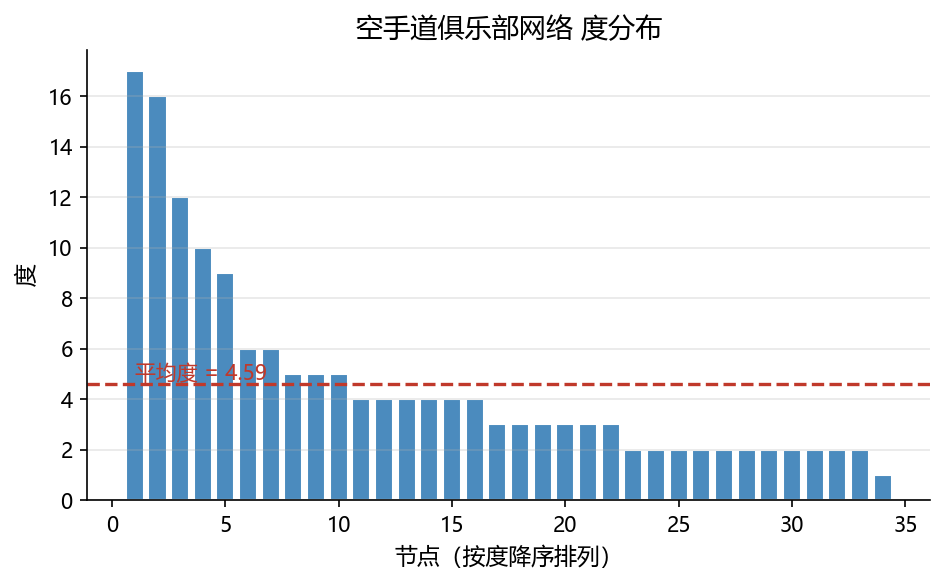
\includegraphics[keepaspectratio,alt={空手道俱乐部 度分布}]{figures/06-networkx/network_case_degree_dist.png}}
\caption{空手道俱乐部 度分布}
\end{figure}

\subsubsection{3) 全局指标}\label{ux5168ux5c40ux6307ux6807}

\begin{Shaded}
\begin{Highlighting}[]
\BuiltInTok{print}\NormalTok{(}\StringTok{"平均聚类系数:"}\NormalTok{, }\BuiltInTok{round}\NormalTok{(nx.average\_clustering(K), }\DecValTok{4}\NormalTok{))}
\BuiltInTok{print}\NormalTok{(}\StringTok{"传递性:"}\NormalTok{, }\BuiltInTok{round}\NormalTok{(nx.transitivity(K), }\DecValTok{4}\NormalTok{))}
\BuiltInTok{print}\NormalTok{(}\StringTok{"平均最短路径长度:"}\NormalTok{, }\BuiltInTok{round}\NormalTok{(nx.average\_shortest\_path\_length(K), }\DecValTok{4}\NormalTok{))}
\BuiltInTok{print}\NormalTok{(}\StringTok{"直径:"}\NormalTok{, nx.diameter(K), }\StringTok{" 半径:"}\NormalTok{, nx.radius(K))}
\NormalTok{bc }\OperatorTok{=}\NormalTok{ nx.betweenness\_centrality(K)}
\NormalTok{top }\OperatorTok{=} \BuiltInTok{sorted}\NormalTok{(bc.items(), key}\OperatorTok{=}\KeywordTok{lambda}\NormalTok{ x: x[}\DecValTok{1}\NormalTok{], reverse}\OperatorTok{=}\VariableTok{True}\NormalTok{)[:}\DecValTok{3}\NormalTok{]}
\BuiltInTok{print}\NormalTok{(}\StringTok{"介数中心性最高前3:"}\NormalTok{, top)}
\end{Highlighting}
\end{Shaded}

\begin{Shaded}
\begin{Highlighting}[]
\NormalTok{平均聚类系数: 0.5706}
\NormalTok{传递性: 0.2557}
\NormalTok{平均最短路径长度: 2.4082}
\NormalTok{直径: 5  半径: 3}
\NormalTok{介数中心性最高前3: [(0, 0.4376), (33, 0.3041), (32, 0.1452)]}
\end{Highlighting}
\end{Shaded}

解读：平均聚类系数较高（0.57），说明``朋友的朋友多是朋友''；但平均最短路径只有
2.41，直径 5，呈现``高聚类 + 短路径''的小世界特征。节点 0 与 33
的介数中心性最高，它们是连接两派之间的``桥梁''。

\subsubsection{4)
社区划分与模块度}\label{ux793eux533aux5212ux5206ux4e0eux6a21ux5757ux5ea6-1}

\begin{Shaded}
\begin{Highlighting}[]
\NormalTok{comms }\OperatorTok{=}\NormalTok{ nxcom.greedy\_modularity\_communities(K)}
\NormalTok{Q }\OperatorTok{=}\NormalTok{ modularity(K, comms)}
\BuiltInTok{print}\NormalTok{(}\StringTok{"社区个数:"}\NormalTok{, }\BuiltInTok{len}\NormalTok{(comms))}
\BuiltInTok{print}\NormalTok{(}\StringTok{"各社区大小:"}\NormalTok{, [}\BuiltInTok{len}\NormalTok{(c) }\ControlFlowTok{for}\NormalTok{ c }\KeywordTok{in}\NormalTok{ comms])}
\BuiltInTok{print}\NormalTok{(}\StringTok{"模块度 Q:"}\NormalTok{, }\BuiltInTok{round}\NormalTok{(Q, }\DecValTok{4}\NormalTok{))}
\end{Highlighting}
\end{Shaded}

\begin{Shaded}
\begin{Highlighting}[]
\NormalTok{社区个数: 3}
\NormalTok{各社区大小: [17, 9, 8]}
\NormalTok{模块度 Q: 0.411}
\end{Highlighting}
\end{Shaded}

Q≈0.41 表示网络存在较明显的社区结构；社区大小
17、9、8，且第一个社区节点编号整体偏大（8,14,15,\ldots,33），与裁判/教练两派吻合。

\subsubsection{5) 最短路径}\label{ux6700ux77edux8defux5f84}

\begin{Shaded}
\begin{Highlighting}[]
\NormalTok{path }\OperatorTok{=}\NormalTok{ nx.shortest\_path(K, source}\OperatorTok{=}\DecValTok{0}\NormalTok{, target}\OperatorTok{=}\DecValTok{33}\NormalTok{)}
\BuiltInTok{print}\NormalTok{(}\StringTok{"0 号到 33 号的最短路径:"}\NormalTok{, path)}
\BuiltInTok{print}\NormalTok{(}\StringTok{"路径长度(边数):"}\NormalTok{, nx.shortest\_path\_length(K, }\DecValTok{0}\NormalTok{, }\DecValTok{33}\NormalTok{))}
\end{Highlighting}
\end{Shaded}

\begin{Shaded}
\begin{Highlighting}[]
\NormalTok{0 号到 33 号的最短路径: [0, 8, 33]}
\NormalTok{路径长度(边数): 2}
\end{Highlighting}
\end{Shaded}

\subsubsection{6) 社区 +
路径可视化}\label{ux793eux533a-ux8defux5f84ux53efux89c6ux5316}

\begin{Shaded}
\begin{Highlighting}[]
\NormalTok{node\_color }\OperatorTok{=}\NormalTok{ \{\}}
\NormalTok{colors }\OperatorTok{=}\NormalTok{ [}\StringTok{"\#4b8bbe"}\NormalTok{, }\StringTok{"\#e07b39"}\NormalTok{, }\StringTok{"\#3a8f4f"}\NormalTok{, }\StringTok{"\#7f5fb5"}\NormalTok{, }\StringTok{"\#c0392b"}\NormalTok{]}
\ControlFlowTok{for}\NormalTok{ ci, cset }\KeywordTok{in} \BuiltInTok{enumerate}\NormalTok{(comms):}
    \ControlFlowTok{for}\NormalTok{ n }\KeywordTok{in}\NormalTok{ cset:}
\NormalTok{        node\_color[n] }\OperatorTok{=}\NormalTok{ colors[ci }\OperatorTok{\%} \BuiltInTok{len}\NormalTok{(colors)]}

\NormalTok{path\_edges }\OperatorTok{=} \BuiltInTok{list}\NormalTok{(}\BuiltInTok{zip}\NormalTok{(path[:}\OperatorTok{{-}}\DecValTok{1}\NormalTok{], path[}\DecValTok{1}\NormalTok{:]))}
\NormalTok{pos }\OperatorTok{=}\NormalTok{ nx.spring\_layout(K, seed}\OperatorTok{=}\DecValTok{42}\NormalTok{)}

\ImportTok{import}\NormalTok{ os}
\NormalTok{plt.rcParams[}\StringTok{"font.sans{-}serif"}\NormalTok{] }\OperatorTok{=}\NormalTok{ [}\StringTok{"Microsoft YaHei"}\NormalTok{, }\StringTok{"SimHei"}\NormalTok{, }\StringTok{"DejaVu Sans"}\NormalTok{]}
\NormalTok{plt.rcParams[}\StringTok{"axes.unicode\_minus"}\NormalTok{] }\OperatorTok{=} \VariableTok{False}
\NormalTok{plt.figure(figsize}\OperatorTok{=}\NormalTok{(}\FloatTok{8.2}\NormalTok{, }\FloatTok{6.2}\NormalTok{))}
\NormalTok{os.makedirs(}\StringTok{"images"}\NormalTok{, exist\_ok}\OperatorTok{=}\VariableTok{True}\NormalTok{)}
\NormalTok{nx.draw\_networkx\_edges(K, pos, alpha}\OperatorTok{=}\FloatTok{0.35}\NormalTok{, edge\_color}\OperatorTok{=}\StringTok{"\#999999"}\NormalTok{, width}\OperatorTok{=}\FloatTok{1.0}\NormalTok{)}
\NormalTok{nx.draw\_networkx\_edges(K, pos, edgelist}\OperatorTok{=}\NormalTok{path\_edges, edge\_color}\OperatorTok{=}\StringTok{"\#c0392b"}\NormalTok{, width}\OperatorTok{=}\FloatTok{3.0}\NormalTok{)}
\NormalTok{nx.draw\_networkx\_nodes(K, pos, node\_size}\OperatorTok{=}\DecValTok{260}\NormalTok{,}
\NormalTok{                       node\_color}\OperatorTok{=}\NormalTok{[node\_color[n] }\ControlFlowTok{for}\NormalTok{ n }\KeywordTok{in}\NormalTok{ K.nodes()],}
\NormalTok{                       edgecolors}\OperatorTok{=}\StringTok{"white"}\NormalTok{, linewidths}\OperatorTok{=}\FloatTok{1.2}\NormalTok{)}
\NormalTok{nx.draw\_networkx\_labels(K, pos, \{n: }\BuiltInTok{str}\NormalTok{(n) }\ControlFlowTok{for}\NormalTok{ n }\KeywordTok{in}\NormalTok{ K.nodes()\}, font\_size}\OperatorTok{=}\DecValTok{8}\NormalTok{)}
\NormalTok{plt.title(}\StringTok{"空手道俱乐部：社区划分 + 0→33 最短路径（红色）"}\NormalTok{)}
\NormalTok{plt.axis(}\StringTok{"off"}\NormalTok{)}
\NormalTok{plt.tight\_layout()}\OperatorTok{;}\NormalTok{ plt.savefig(}\StringTok{"figures/06{-}networkx/network\_case\_communities.png"}\NormalTok{)}
\BuiltInTok{print}\NormalTok{(}\StringTok{"已保存 communities"}\NormalTok{)}
\end{Highlighting}
\end{Shaded}

\begin{figure}
\centering
\pandocbounded{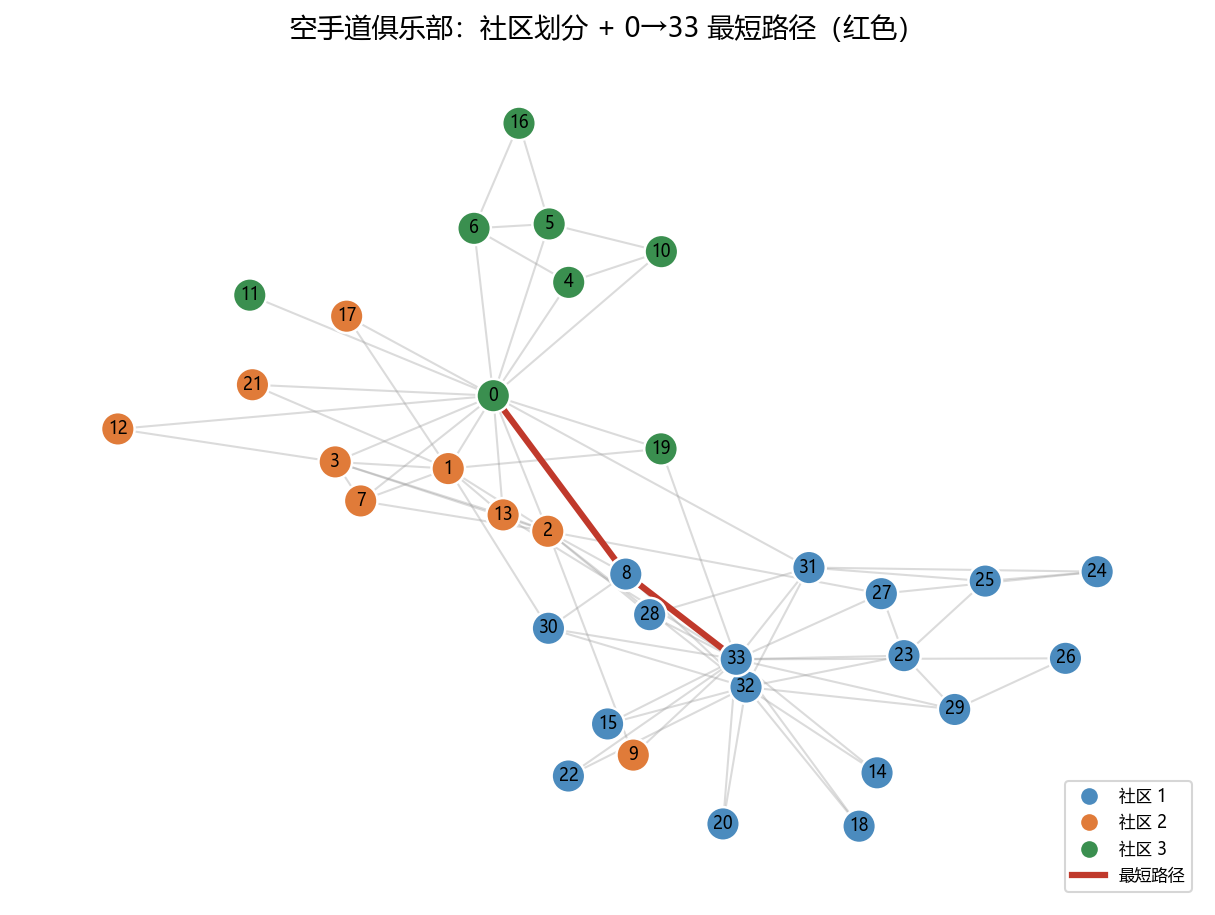
\includegraphics[keepaspectratio,alt={空手道俱乐部 社区划分与最短路径}]{figures/06-networkx/network_case_communities.png}}
\caption{空手道俱乐部 社区划分与最短路径}
\end{figure}

\subsubsection{主要用法 / API}\label{ux4e3bux8981ux7528ux6cd5-api-27}

{\def\LTcaptype{none} % do not increment counter
\begin{longtable}[]{@{}
  >{\raggedright\arraybackslash}p{(\linewidth - 4\tabcolsep) * \real{0.3333}}
  >{\raggedright\arraybackslash}p{(\linewidth - 4\tabcolsep) * \real{0.3333}}
  >{\raggedright\arraybackslash}p{(\linewidth - 4\tabcolsep) * \real{0.3333}}@{}}
\toprule\noalign{}
\begin{minipage}[b]{\linewidth}\raggedright
需求
\end{minipage} & \begin{minipage}[b]{\linewidth}\raggedright
写法
\end{minipage} & \begin{minipage}[b]{\linewidth}\raggedright
说明
\end{minipage} \\
\midrule\noalign{}
\endhead
\bottomrule\noalign{}
\endlastfoot
载入经典网络 & \texttt{nx.karate\_club\_graph()} & 34 节点 78 边 \\
度分布 &
\texttt{sorted({[}d\ for\ \_,\ d\ in\ K.degree(){]},\ reverse=True)} &
长尾/无标度特征 \\
全局指标 & \texttt{nx.average\_clustering} / \texttt{nx.transitivity} /
\texttt{nx.average\_shortest\_path\_length} & 小世界效应 \\
社区划分 & \texttt{nxcom.greedy\_modularity\_communities(K)} &
返回社区集合 \\
模块度 & \texttt{modularity(K,\ comms)} & 划分质量 Q \\
最短路径 & \texttt{nx.shortest\_path(K,\ 0,\ 33)} & 无权最短路 \\
可视化 & \texttt{nx.draw\_networkx\_*} +
\texttt{spring\_layout(K,\ seed=42)} & 固定布局便于复现 \\
\end{longtable}
}

\subsubsection{常见错误}\label{ux5e38ux89c1ux9519ux8bef-27}

\begin{enumerate}
\def\labelenumi{\arabic{enumi}.}
\tightlist
\item
  忘记导入社区子模块：社区函数在 \texttt{networkx.algorithms.community}
  下，需要
  \texttt{from\ networkx.algorithms\ import\ community\ as\ nxcom}。
\item
  把模块度 Q 当成``越大越绝对正确''：Q 是相对指标，0.41 对 34
  节点网络已算不错，但不同算法或 seed 可能得到不同社区数。
\item
  \texttt{spring\_layout} 不传
  \texttt{seed}：每次布局不同，截图/复现对不上。
\item
  把``度分布降序图''误当成直方图：这里 x
  轴是``按度排序的节点编号''，并不是度数分箱。
\end{enumerate}

\subsubsection{拓展 / 跟练}\label{ux62d3ux5c55-ux8ddfux7ec3-15}

\begin{enumerate}
\def\labelenumi{\arabic{enumi}.}
\tightlist
\item
  分别计算 0 号与 33
  号的度、介数中心性、接近中心性，比较两者谁更像``中心''。
\item
  用 \texttt{nx.community.louvain\_communities(K,\ seed=42)}
  划分，比较社区个数与 Q 值。
\item
  把``0→33
  最短路径''推广成``所有点对平均最短路径''，并解释``六度分隔''。
\item
  用 \texttt{nx.to\_numpy\_array(K)} 得到 34x34
  邻接矩阵，验证对称；再交给 SciPy 做特征值（可选）。
\end{enumerate}

\begin{center}\rule{0.5\linewidth}{0.5pt}\end{center}

\subsection{案例结论}\label{ux6848ux4f8bux7ed3ux8bba}

\begin{itemize}
\tightlist
\item
  度分布有明显``长尾''：少数节点度很高（节点 0
  度=17），符合社交网络的无标度特征；
\item
  高聚类系数、短平均路径，说明该网络具有小世界效应；
\item
  社区检测给出 3 个社区、Q≈0.41，划分质量较好；
\item
  最短路径 0→8→33
  表明两位``领袖''其实只隔一个中间人，再次体现``六度分隔''。
\end{itemize}

\subsection{拓展任务}\label{ux62d3ux5c55ux4efbux52a1-6}

\begin{enumerate}
\def\labelenumi{\arabic{enumi}.}
\tightlist
\item
  分别计算 0 号与 33
  号节点的度、介数中心性、接近中心性，比较两者谁更像``中心''；
\item
  修改 seed 重新布局，观察社区/路径是否变化（应不变，因为 graph
  本身不变，只有节点画的位置变）；
\item
  用 nx.connected\_components
  检查该网络是否连通；若不连通，找出孤立分量；
\item
  用
  louvain\_communities（networkx.algorithms.community.louvain\_communities）划分，比较社区个数与
  Q 值。
\end{enumerate}

\subsection{本章综合练习（上机任务）}\label{ux672cux7ae0ux7efcux5408ux7ec3ux4e60ux4e0aux673aux4efbux52a1-2}

\begin{enumerate}
\def\labelenumi{\arabic{enumi}.}
\tightlist
\item
  用 erdos\_renyi\_graph(100, 0.05, seed=1)
  生成随机网络，计算平均聚类系数与平均最短路径，与 karate
  网络对比，说明``小世界''差异；
\item
  在 karate\_club\_graph 上分别计算 average\_clustering 与
  transitivity，并解释两者为何不同；
\item
  把本案例整理成一个 .ipynb，写出 3 句结论。
\end{enumerate}

\subsection{延伸阅读}\label{ux5ef6ux4f38ux9605ux8bfb-29}

\begin{itemize}
\tightlist
\item
  Zachary
  空手道俱乐部数据集说明：\href{https://networkx.org/documentation/stable/reference/generated/networkx.generators.social.karate_club_graph.html}{链接}
\item
  NetworkX
  社区检测模块：\href{https://networkx.org/documentation/stable/reference/algorithms/community.html}{链接}
\item
  NetworkX
  布局算法：\href{https://networkx.org/documentation/stable/reference/drawing.html}{链接}
\end{itemize}

\section{05
常见误区与技巧}\label{ux5e38ux89c1ux8befux533aux4e0eux6280ux5de7-5}

\begin{quote}
本章为新增``查漏补缺''页：把学生最容易踩的坑集中列出，并给出正确写法与性能/调试技巧。
\end{quote}

\subsection{1.
高频误区速查表}\label{ux9ad8ux9891ux8befux533aux901fux67e5ux8868-5}

{\def\LTcaptype{none} % do not increment counter
\begin{longtable}[]{@{}
  >{\raggedright\arraybackslash}p{(\linewidth - 6\tabcolsep) * \real{0.2500}}
  >{\raggedright\arraybackslash}p{(\linewidth - 6\tabcolsep) * \real{0.2500}}
  >{\raggedright\arraybackslash}p{(\linewidth - 6\tabcolsep) * \real{0.2500}}
  >{\raggedright\arraybackslash}p{(\linewidth - 6\tabcolsep) * \real{0.2500}}@{}}
\toprule\noalign{}
\begin{minipage}[b]{\linewidth}\raggedright
\#
\end{minipage} & \begin{minipage}[b]{\linewidth}\raggedright
误区 / 错误写法
\end{minipage} & \begin{minipage}[b]{\linewidth}\raggedright
正确做法
\end{minipage} & \begin{minipage}[b]{\linewidth}\raggedright
原因
\end{minipage} \\
\midrule\noalign{}
\endhead
\bottomrule\noalign{}
\endlastfoot
1 & 把 G.nodes() / G.edges() 当普通列表直接修改 & 用 list(G.nodes())
转列表；改图用 add\_node / remove\_node & 返回的是视图对象 \\
2 & 在有向图上用 G.neighbors(2) 当``指向 2 的节点'' & 用
DG.predecessors(2) 找前驱，DG.successors(2) 找后继 & 邻居 = 后继 \\
3 & zip(G.nodes(), G.in\_degree(), G.out\_degree()) 解包 & 用
dict(DG.in\_degree()) 或 DG.in\_degree(node) & in\_degree 返回 (节点,
度数) 对 \\
4 & add\_edge(u, v, 10) 当权重 & add\_weighted\_edges\_from 或
add\_edge(u, v, weight=10) & 三参数不是权重签名 \\
5 & 随机图不设 seed & nx.erdos\_renyi\_graph(10, 0.3, seed=42) &
结果不可复现 \\
6 & 把 average\_shortest\_path\_length 用在``有权图''上却不带 weight &
加 weight=``weight'' 参数；无权图则默认 & 默认按无权（每条边=1）计算 \\
7 & 用 Dijkstra 处理负权边 & 改用 bellman\_ford\_path / floyd\_warshall
& Dijkstra 依赖非负权 \\
8 & 在``数三角形/算模块度''时以为结果为整数 & triangles 是
dict，总三角形数 = sum//3；模块度 Q 是 float & 不同数值语义 \\
9 & 认为 minimum\_spanning\_tree 结论就是``最短路径'' &
分清``连通所有点总权重最小''与``两点间距离最小'' & 目标不同 \\
10 & 用 nx.diameter 对不连通图 & 先判断
is\_connected，或按连通分量分别算 & 不连通无有限直径 \\
11 & 用 nx.to\_numpy\_array 得到的是 float 矩阵 & 需要整数可转
A.astype(int) & 默认 float64 \\
12 & 社区检测结果当成唯一正确解 & 多算法多 seed 交叉验证，报告 Q
值而非``社区是\ldots\ldots'' & 社区划分非唯一 \\
\end{longtable}
}

\subsection{2. 原理级注意点}\label{ux539fux7406ux7ea7ux6ce8ux610fux70b9}

\subsubsection{2.1 视图 vs
数据结构}\label{ux89c6ux56fe-vs-ux6570ux636eux7ed3ux6784}

G.nodes() 与 G.edges()
是视图对象，支持迭代与成员判断，但不支持``直接赋值''。要得到稳定快照用：

\begin{Shaded}
\begin{Highlighting}[]
\ImportTok{import}\NormalTok{ networkx }\ImportTok{as}\NormalTok{ nx}
\NormalTok{G }\OperatorTok{=}\NormalTok{ nx.Graph()}
\NormalTok{G.add\_edges\_from([(}\DecValTok{1}\NormalTok{, }\DecValTok{2}\NormalTok{), (}\DecValTok{2}\NormalTok{, }\DecValTok{3}\NormalTok{)])}

\NormalTok{node\_list }\OperatorTok{=} \BuiltInTok{list}\NormalTok{(G.nodes())}
\NormalTok{edge\_list }\OperatorTok{=} \BuiltInTok{list}\NormalTok{(G.edges())}
\NormalTok{degree\_view }\OperatorTok{=} \BuiltInTok{dict}\NormalTok{(G.degree())}
\BuiltInTok{print}\NormalTok{(node\_list, edge\_list, degree\_view)}
\end{Highlighting}
\end{Shaded}

\subsubsection{2.2
有向图连通性的``方向坑''}\label{ux6709ux5411ux56feux8fdeux901aux6027ux7684ux65b9ux5411ux5751}

有向图的 is\_connected 不存在；要用 is\_strongly\_connected 与
is\_weakly\_connected。把无向图用 nx.DiGraph(G)
转换后，每条无向边会变成双向两条边，所以结论可能与你直觉不同。

\subsubsection{2.3 加权 vs 无权}\label{ux52a0ux6743-vs-ux65e0ux6743}

大多网络函数默认按``无权''处理（每条边权重=1）。一旦图带 weight
属性，要么显式传
weight=``weight''，要么接受默认``无权''结果。二者结果可能完全不同。

\subsection{3. 性能技巧}\label{ux6027ux80fdux6280ux5de7-4}

\begin{itemize}
\tightlist
\item
  \textbf{用生成器造图}：path\_graph / cycle\_graph /
  erdos\_renyi\_graph 比手动 add\_node 循环快得多；
\item
  \textbf{批量加边}：add\_edges\_from /
  add\_weighted\_edges\_from，不要一条条 add\_edge；
\item
  \textbf{中心性按需计算}：betweenness\_centrality
  默认精确算法在大图很慢；可用 k 参数（k
  个随机源）近似，或只计算关心的节点子集；
\item
  \textbf{社区检测选算法}：greedy\_modularity\_communities
  适合中等规模；超大图可用 louvain\_communities（更快）；
\item
  \textbf{复用图对象}：对同一张图反复调用算法时，先复制为
  G.copy()，避免原地修改影响后续分析；
\item
  \textbf{大图用稀疏结构}：需要把邻接矩阵交给 SciPy 时，用
  nx.to\_scipy\_sparse\_array(G) 得到稀疏矩阵，节省内存（若安装了
  scipy）。
\end{itemize}

\subsection{4. 调试建议}\label{ux8c03ux8bd5ux5efaux8bae-5}

\begin{enumerate}
\def\labelenumi{\arabic{enumi}.}
\tightlist
\item
  先打印 G.number\_of\_nodes()、G.number\_of\_edges()，确认图建对了；
\item
  用 sorted(G.nodes()) 检查节点是否被意外``自动补全''；
\item
  报路径错误时先判断连通性：\texttt{nx.is\_connected(G)}（有向用
  \texttt{is\_strongly\_connected}）；
\item
  带权问题先把边打印出来：\texttt{G.edges(data=True)}，确认 weight
  属性名与数值；
\item
  较慢的算法先在小图上验证（如 path\_graph(10)）再加到大数据；
\item
  绘图布局不稳定时，给 spring\_layout 传 seed，便于复现。
\end{enumerate}

\subsection{5.
本章小结（自测）}\label{ux672cux7ae0ux5c0fux7ed3ux81eaux6d4b-3}

\begin{itemize}
\tightlist
\item[$\square$]
  能区分 Graph 与 DiGraph，说出 neighbors / predecessors / successors
  的差异；
\item[$\square$]
  能给图加节点属性、边权重，并用 nodes(data=True)、edges(data=True)
  查看；
\item[$\square$]
  能说出度/度分布、聚类系数、传递性、介数中心性、接近中心性、模块度的含义；
\item[$\square$]
  能根据图特性为最短路径选择 Dijkstra / Bellman-Ford / Floyd-Warshall；
\item[$\square$]
  能用 minimum\_spanning\_tree 求 MST 并算总权重；
\item[$\square$]
  能完成 04 综合案例并在图上可视化社区与最短路径。
\end{itemize}

\subsection{延伸阅读}\label{ux5ef6ux4f38ux9605ux8bfb-30}

\begin{itemize}
\tightlist
\item
  NetworkX
  官方``算法总览''：\href{https://networkx.org/documentation/stable/reference/algorithms/index.html}{链接}
\item
  NetworkX
  官方绘图指南：\href{https://networkx.org/documentation/stable/reference/drawing.html}{链接}
\item
  NetworkX
  官方``性能提示''与稀疏表示：\href{https://networkx.org/documentation/stable/reference/convert.html}{链接}
\end{itemize}

\newpage

%% 由 build/emit_tex.py 生成（生成物，勿手改）；定制请放 user_style.tex / user_meta.yaml
\chapter{第 7 章 ·
Statsmodels及其基本使用}\label{ux7b2c-7-ux7ae0-statsmodelsux53caux5176ux57faux672cux4f7fux7528}

\section{01
方差分析与回归}\label{ux65b9ux5deeux5206ux6790ux4e0eux56deux5f52}

\begin{quote}
本节对应原版 7.1 的内容，并增补目标、诊断、GLM、WLS 与思考题。
配套图：figures/07-statsmodels/regression\_ols.png、figures/07-statsmodels/anova\_boxes.png、figures/07-statsmodels/qq\_resid.png（由
build/make\_chap7\_figures.py 生成）。
\end{quote}

\subsection{本节目标}\label{ux672cux8282ux76eeux6807-26}

\begin{itemize}
\tightlist
\item
  会用 statsmodels.api.OLS 与 add\_constant 做一元/多元线性回归，并读懂
  summary()；
\item
  会用公式 API ols(`y \textasciitilde{} x', data=df)，理解分类变量
  C(\ldots) 与交互项写法；
\item
  会用 anova\_lm 做单因素方差分析，解读 F 统计量与 P 值；
\item
  会用 GLM + Binomial 做二分类 Logit 回归并得到概率；
\item
  会做基本回归诊断（残差 QQ 图、JB 统计量）与异方差处理（WLS）。
\end{itemize}

\subsection{先修}\label{ux5148ux4fee-19}

\begin{itemize}
\tightlist
\item
  Python 基础、NumPy 数组、Pandas
  DataFrame；了解最小二乘与回归的统计含义。
\item
  已安装 statsmodels（见章 README）。
\end{itemize}

\subsection{官方文档/参考入口}\label{ux5b98ux65b9ux6587ux6863ux53c2ux8003ux5165ux53e3-5}

{\def\LTcaptype{none} % do not increment counter
\begin{longtable}[]{@{}
  >{\raggedright\arraybackslash}p{(\linewidth - 4\tabcolsep) * \real{0.3333}}
  >{\raggedright\arraybackslash}p{(\linewidth - 4\tabcolsep) * \real{0.3333}}
  >{\raggedright\arraybackslash}p{(\linewidth - 4\tabcolsep) * \real{0.3333}}@{}}
\toprule\noalign{}
\begin{minipage}[b]{\linewidth}\raggedright
内容
\end{minipage} & \begin{minipage}[b]{\linewidth}\raggedright
链接
\end{minipage} & \begin{minipage}[b]{\linewidth}\raggedright
说明
\end{minipage} \\
\midrule\noalign{}
\endhead
\bottomrule\noalign{}
\endlastfoot
OLS（回归模型） &
\href{https://www.statsmodels.org/stable/generated/statsmodels.regression.linear_model.OLS.html}{链接}
& 最小二乘回归主接口 \\
Regressions 官方教程 &
\href{https://www.statsmodels.org/stable/regression.html}{链接} &
回归模型总览 \\
公式 API & \href{https://www.statsmodels.org/stable/formula.html}{链接}
& ols(`y \textasciitilde{} x', data=\ldots) 语法 \\
anova\_lm &
\href{https://www.statsmodels.org/stable/generated/statsmodels.stats.anova.anova_lm.html}{链接}
& 对 OLS 结果做方差分析 \\
GLM &
\href{https://www.statsmodels.org/stable/generated/statsmodels.genmod.generalized_linear_model.GLM.html}{链接}
& 广义线性模型 \\
WLS &
\href{https://www.statsmodels.org/stable/generated/statsmodels.regression.linear_model.WLS.html}{链接}
& 加权最小二乘 \\
\end{longtable}
}

\begin{center}\rule{0.5\linewidth}{0.5pt}\end{center}

\subsection{1 方差分析（ANOVA）}\label{ux65b9ux5deeux5206ux6790anova}

\subsubsection{1.1 概念}\label{ux6982ux5ff5}

方差分析（ANOVA, Analysis of
Variance）用来检验\textbf{多个组的均值是否显著不同}。其核心思路是把总离差平方和
\(SS_{tot}\) 分解为\textbf{组间平方和} \(SS_{between}\)
与\textbf{组内平方和} \(SS_{within}\)，并构造 F 统计量：

\[
F = \frac{SS_{between}/(k-1)}{SS_{within}/(N-k)}
\]

其中 \(k\) 为组数，\(N\) 为总样本数。若 \(F\) 很大（对应 P
值很小），说明组间差异显著，各组的总体均值不全相等。

Statsmodels 通常先用 OLS
拟合一个``将分组变量视为分类自变量''的模型，再用 anova\_lm
输出方差分析表。

\subsubsection{1.2
单因素方差分析示例}\label{ux5355ux56e0ux7d20ux65b9ux5deeux5206ux6790ux793aux4f8b}

构造三个组（A/B/C），每组均值分别为 0、1、2，并加噪声：

\begin{Shaded}
\begin{Highlighting}[]
\ImportTok{import}\NormalTok{ numpy }\ImportTok{as}\NormalTok{ np}
\ImportTok{import}\NormalTok{ pandas }\ImportTok{as}\NormalTok{ pd}
\ImportTok{import}\NormalTok{ statsmodels.api }\ImportTok{as}\NormalTok{ sm}
\ImportTok{from}\NormalTok{ statsmodels.formula.api }\ImportTok{import}\NormalTok{ ols}
\ImportTok{import}\NormalTok{ matplotlib.pyplot }\ImportTok{as}\NormalTok{ plt}

\NormalTok{plt.rcParams[}\StringTok{\textquotesingle{}font.sans{-}serif\textquotesingle{}}\NormalTok{] }\OperatorTok{=}\NormalTok{ [}\StringTok{\textquotesingle{}Microsoft YaHei\textquotesingle{}}\NormalTok{, }\StringTok{\textquotesingle{}SimHei\textquotesingle{}}\NormalTok{, }\StringTok{\textquotesingle{}DejaVu Sans\textquotesingle{}}\NormalTok{]}
\NormalTok{plt.rcParams[}\StringTok{\textquotesingle{}axes.unicode\_minus\textquotesingle{}}\NormalTok{] }\OperatorTok{=} \VariableTok{False}

\NormalTok{rng }\OperatorTok{=}\NormalTok{ np.random.default\_rng(}\DecValTok{1}\NormalTok{)}
\NormalTok{n }\OperatorTok{=} \DecValTok{12}
\NormalTok{df }\OperatorTok{=}\NormalTok{ pd.DataFrame(\{}
    \StringTok{\textquotesingle{}group\textquotesingle{}}\NormalTok{: [}\StringTok{\textquotesingle{}A\textquotesingle{}}\NormalTok{]}\OperatorTok{*}\NormalTok{n }\OperatorTok{+}\NormalTok{ [}\StringTok{\textquotesingle{}B\textquotesingle{}}\NormalTok{]}\OperatorTok{*}\NormalTok{n }\OperatorTok{+}\NormalTok{ [}\StringTok{\textquotesingle{}C\textquotesingle{}}\NormalTok{]}\OperatorTok{*}\NormalTok{n,}
    \StringTok{\textquotesingle{}y\textquotesingle{}}\NormalTok{: np.r\_[rng.normal(}\DecValTok{0}\NormalTok{,}\DecValTok{1}\NormalTok{,n), rng.normal(}\DecValTok{1}\NormalTok{,}\DecValTok{1}\NormalTok{,n), rng.normal(}\DecValTok{2}\NormalTok{,}\DecValTok{1}\NormalTok{,n)]}
\NormalTok{\})}
\BuiltInTok{print}\NormalTok{(df.groupby(}\StringTok{\textquotesingle{}group\textquotesingle{}}\NormalTok{)[}\StringTok{\textquotesingle{}y\textquotesingle{}}\NormalTok{].mean().}\BuiltInTok{round}\NormalTok{(}\DecValTok{4}\NormalTok{))}

\NormalTok{model }\OperatorTok{=}\NormalTok{ ols(}\StringTok{\textquotesingle{}y \textasciitilde{} C(group)\textquotesingle{}}\NormalTok{, data}\OperatorTok{=}\NormalTok{df).fit()}
\NormalTok{anova\_res }\OperatorTok{=}\NormalTok{ sm.stats.anova\_lm(model, typ}\OperatorTok{=}\DecValTok{1}\NormalTok{)}
\BuiltInTok{print}\NormalTok{(anova\_res)}
\end{Highlighting}
\end{Shaded}

运行结果：

\begin{Shaded}
\begin{Highlighting}[]
\NormalTok{group}
\NormalTok{A    0.2354}
\NormalTok{B    0.9966}
\NormalTok{C    1.9345}
\NormalTok{Name: y, dtype: float64}

\NormalTok{            df     sum\_sq   mean\_sq         F    PR(\textgreater{}F)}
\NormalTok{C(group)   2.0  17.386102  8.693051  9.297656  0.000627}
\NormalTok{Residual  33.0  30.854088  0.934972       NaN       NaN}
\end{Highlighting}
\end{Shaded}

\begin{figure}
\centering
\pandocbounded{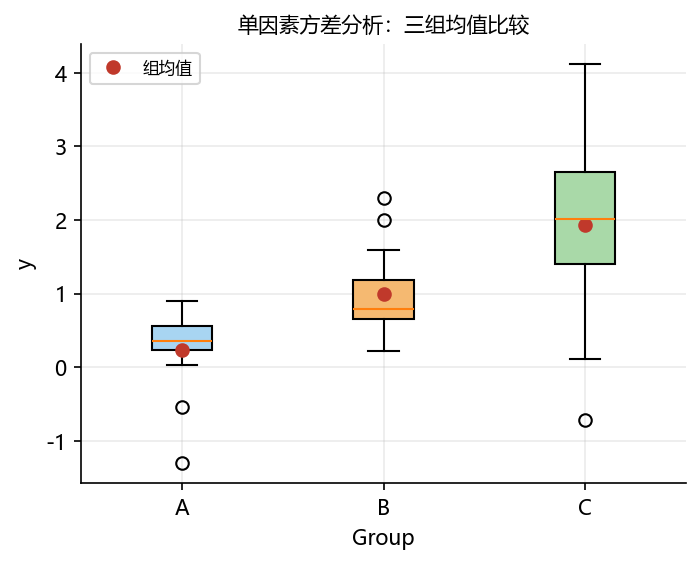
\includegraphics[keepaspectratio,alt={三个组的箱线图}]{figures/07-statsmodels/anova_boxes.png}}
\caption{三个组的箱线图}
\end{figure}

\subsubsection{1.3 解读}\label{ux89e3ux8bfb}

\begin{itemize}
\tightlist
\item
  C(group) 告诉 ols 把 group 当作\textbf{分类变量}，展开成虚拟变量；
\item
  PR(\textgreater F) 是 F 检验的 P 值，本例 0.000627 \textless{}
  0.05，说明三组均值\textbf{存在显著差异}；
\item
  sum\_sq 是平方和，mean\_sq = sum\_sq / df，F = 组间 mean\_sq / 组内
  mean\_sq。
\end{itemize}

\begin{quote}
多做几组对比时，anova\_lm 的 typ 可切换 I/II/III
型平方和；单因素情形三者等价。
\end{quote}

\subsection{案例卡
1：单因素方差分析------三种肥料对产量差异是否显著}\label{ux6848ux4f8bux5361-1ux5355ux56e0ux7d20ux65b9ux5deeux5206ux6790ux4e09ux79cdux80a5ux6599ux5bf9ux4ea7ux91cfux5deeux5f02ux662fux5426ux663eux8457}

\subsubsection{目标}\label{ux76eeux6807-27}

在田间试验里，把同一作物种在 45 块小地上，分别施 A、B、C
三种肥料，每种肥料 15
块地，记录每块地产量。我们要用\textbf{单因素方差分析}（One-Way
ANOVA）回答：三种肥料的平均产量差异，究竟是\textbf{真实的处理效应}，还是\textbf{抽样噪声}造成的巧合。核心统计量是
F 值与其 P 值。

\subsubsection{代码}\label{ux4ee3ux7801-28}

\begin{Shaded}
\begin{Highlighting}[]
\ImportTok{import}\NormalTok{ numpy }\ImportTok{as}\NormalTok{ np}
\ImportTok{import}\NormalTok{ pandas }\ImportTok{as}\NormalTok{ pd}
\ImportTok{import}\NormalTok{ statsmodels.api }\ImportTok{as}\NormalTok{ sm}
\ImportTok{from}\NormalTok{ statsmodels.formula.api }\ImportTok{import}\NormalTok{ ols}
\ImportTok{import}\NormalTok{ matplotlib.pyplot }\ImportTok{as}\NormalTok{ plt}
\ImportTok{import}\NormalTok{ os}

\NormalTok{plt.rcParams[}\StringTok{\textquotesingle{}font.sans{-}serif\textquotesingle{}}\NormalTok{] }\OperatorTok{=}\NormalTok{ [}\StringTok{\textquotesingle{}Microsoft YaHei\textquotesingle{}}\NormalTok{, }\StringTok{\textquotesingle{}SimHei\textquotesingle{}}\NormalTok{, }\StringTok{\textquotesingle{}DejaVu Sans\textquotesingle{}}\NormalTok{]}
\NormalTok{plt.rcParams[}\StringTok{\textquotesingle{}axes.unicode\_minus\textquotesingle{}}\NormalTok{] }\OperatorTok{=} \VariableTok{False}
\NormalTok{np.set\_printoptions(precision}\OperatorTok{=}\DecValTok{4}\NormalTok{, suppress}\OperatorTok{=}\VariableTok{True}\NormalTok{)}
\NormalTok{pd.set\_option(}\StringTok{\textquotesingle{}display.width\textquotesingle{}}\NormalTok{, }\DecValTok{100}\NormalTok{)}

\NormalTok{rng }\OperatorTok{=}\NormalTok{ np.random.default\_rng(}\DecValTok{42}\NormalTok{)}
\NormalTok{n }\OperatorTok{=} \DecValTok{15}
\NormalTok{a }\OperatorTok{=}\NormalTok{ rng.normal(}\DecValTok{50}\NormalTok{, }\DecValTok{6}\NormalTok{, n)}
\NormalTok{b }\OperatorTok{=}\NormalTok{ rng.normal(}\DecValTok{55}\NormalTok{, }\DecValTok{6}\NormalTok{, n)}
\NormalTok{c }\OperatorTok{=}\NormalTok{ rng.normal(}\DecValTok{60}\NormalTok{, }\DecValTok{6}\NormalTok{, n)}
\NormalTok{df }\OperatorTok{=}\NormalTok{ pd.DataFrame(\{}\StringTok{\textquotesingle{}fertilizer\textquotesingle{}}\NormalTok{: [}\StringTok{\textquotesingle{}A\textquotesingle{}}\NormalTok{]}\OperatorTok{*}\NormalTok{n }\OperatorTok{+}\NormalTok{ [}\StringTok{\textquotesingle{}B\textquotesingle{}}\NormalTok{]}\OperatorTok{*}\NormalTok{n }\OperatorTok{+}\NormalTok{ [}\StringTok{\textquotesingle{}C\textquotesingle{}}\NormalTok{]}\OperatorTok{*}\NormalTok{n,}
                   \StringTok{\textquotesingle{}out\textquotesingle{}}\NormalTok{: np.r\_[a, b, c]\})}

\BuiltInTok{print}\NormalTok{(df.groupby(}\StringTok{\textquotesingle{}fertilizer\textquotesingle{}}\NormalTok{)[}\StringTok{\textquotesingle{}out\textquotesingle{}}\NormalTok{].mean().}\BuiltInTok{round}\NormalTok{(}\DecValTok{2}\NormalTok{))}

\NormalTok{model }\OperatorTok{=}\NormalTok{ ols(}\StringTok{\textquotesingle{}out \textasciitilde{} C(fertilizer)\textquotesingle{}}\NormalTok{, data}\OperatorTok{=}\NormalTok{df).fit()}
\NormalTok{anova }\OperatorTok{=}\NormalTok{ sm.stats.anova\_lm(model, typ}\OperatorTok{=}\DecValTok{1}\NormalTok{)}
\BuiltInTok{print}\NormalTok{(}\StringTok{\textquotesingle{}F = }\SpecialCharTok{\%.3f}\StringTok{\textquotesingle{}} \OperatorTok{\%}\NormalTok{ anova[}\StringTok{\textquotesingle{}F\textquotesingle{}}\NormalTok{].iloc[}\DecValTok{0}\NormalTok{])}
\BuiltInTok{print}\NormalTok{(}\StringTok{\textquotesingle{}P = }\SpecialCharTok{\%.3g}\StringTok{\textquotesingle{}} \OperatorTok{\%}\NormalTok{ anova[}\StringTok{\textquotesingle{}PR(\textgreater{}F)\textquotesingle{}}\NormalTok{].iloc[}\DecValTok{0}\NormalTok{])}
\BuiltInTok{print}\NormalTok{(}\StringTok{\textquotesingle{}SS\_between = }\SpecialCharTok{\%.3f}\StringTok{\textquotesingle{}} \OperatorTok{\%}\NormalTok{ anova[}\StringTok{\textquotesingle{}sum\_sq\textquotesingle{}}\NormalTok{].iloc[}\DecValTok{0}\NormalTok{])}
\BuiltInTok{print}\NormalTok{(}\StringTok{\textquotesingle{}SS\_within = }\SpecialCharTok{\%.3f}\StringTok{\textquotesingle{}} \OperatorTok{\%}\NormalTok{ anova[}\StringTok{\textquotesingle{}sum\_sq\textquotesingle{}}\NormalTok{].iloc[}\DecValTok{1}\NormalTok{])}
\BuiltInTok{print}\NormalTok{(}\StringTok{\textquotesingle{}df\_between =\textquotesingle{}}\NormalTok{, anova[}\StringTok{\textquotesingle{}df\textquotesingle{}}\NormalTok{].iloc[}\DecValTok{0}\NormalTok{], }\StringTok{\textquotesingle{} df\_within =\textquotesingle{}}\NormalTok{, anova[}\StringTok{\textquotesingle{}df\textquotesingle{}}\NormalTok{].iloc[}\DecValTok{1}\NormalTok{])}

\NormalTok{os.makedirs(}\StringTok{\textquotesingle{}images\textquotesingle{}}\NormalTok{, exist\_ok}\OperatorTok{=}\VariableTok{True}\NormalTok{)}
\NormalTok{plt.figure(figsize}\OperatorTok{=}\NormalTok{(}\FloatTok{5.6}\NormalTok{, }\FloatTok{3.8}\NormalTok{))}
\NormalTok{bp }\OperatorTok{=}\NormalTok{ plt.boxplot([a, b, c], tick\_labels}\OperatorTok{=}\NormalTok{[}\StringTok{\textquotesingle{}A\textquotesingle{}}\NormalTok{, }\StringTok{\textquotesingle{}B\textquotesingle{}}\NormalTok{, }\StringTok{\textquotesingle{}C\textquotesingle{}}\NormalTok{], patch\_artist}\OperatorTok{=}\VariableTok{True}\NormalTok{)}
\ControlFlowTok{for}\NormalTok{ patch, color }\KeywordTok{in} \BuiltInTok{zip}\NormalTok{(bp[}\StringTok{\textquotesingle{}boxes\textquotesingle{}}\NormalTok{], [}\StringTok{\textquotesingle{}\#a8d5f2\textquotesingle{}}\NormalTok{, }\StringTok{\textquotesingle{}\#f5b971\textquotesingle{}}\NormalTok{, }\StringTok{\textquotesingle{}\#a9d9a8\textquotesingle{}}\NormalTok{]):}
\NormalTok{    patch.set\_facecolor(color)}
\NormalTok{plt.plot([}\DecValTok{1}\NormalTok{, }\DecValTok{2}\NormalTok{, }\DecValTok{3}\NormalTok{], [a.mean(), b.mean(), c.mean()], marker}\OperatorTok{=}\StringTok{\textquotesingle{}o\textquotesingle{}}\NormalTok{, color}\OperatorTok{=}\StringTok{\textquotesingle{}\#c0392b\textquotesingle{}}\NormalTok{,}
\NormalTok{         ls}\OperatorTok{=}\StringTok{\textquotesingle{}\textquotesingle{}}\NormalTok{, label}\OperatorTok{=}\StringTok{\textquotesingle{}组均值\textquotesingle{}}\NormalTok{)}
\NormalTok{plt.legend(fontsize}\OperatorTok{=}\DecValTok{8}\NormalTok{)}
\NormalTok{plt.grid(alpha}\OperatorTok{=}\FloatTok{0.25}\NormalTok{)}
\NormalTok{plt.savefig(}\StringTok{\textquotesingle{}figures/07{-}statsmodels/case1\_fertilizer\_anova.png\textquotesingle{}}\NormalTok{, dpi}\OperatorTok{=}\DecValTok{150}\NormalTok{)}
\NormalTok{plt.close()}
\BuiltInTok{print}\NormalTok{(}\StringTok{\textquotesingle{}saved figures/07{-}statsmodels/case1\_fertilizer\_anova.png\textquotesingle{}}\NormalTok{)}
\end{Highlighting}
\end{Shaded}

\subsubsection{运行结果（已运行核验）}\label{ux8fd0ux884cux7ed3ux679cux5df2ux8fd0ux884cux6838ux9a8c-26}

\begin{Shaded}
\begin{Highlighting}[]
\NormalTok{fertilizer}
\NormalTok{A    49.98}
\NormalTok{B    55.22}
\NormalTok{C    60.80}
\NormalTok{Name: out, dtype: float64}
\NormalTok{F = 18.455}
\NormalTok{P = 1.77e{-}06}
\NormalTok{SS\_between = 877.288}
\NormalTok{SS\_within = 998.289}
\NormalTok{df\_between = 2.0  df\_within = 42.0}
\NormalTok{saved figures/07{-}statsmodels/case1\_fertilizer\_anova.png}
\end{Highlighting}
\end{Shaded}

\subsubsection{讲解}\label{ux8bb2ux89e3-26}

\textbf{一句话解释}：把 45
块地的产量按``肥料''分成三堆，先看每堆平均数，再看堆与堆之间的差距，是否大到不像是``随机抽签运气好/坏''造成的。

\begin{enumerate}
\def\labelenumi{\arabic{enumi}.}
\tightlist
\item
  \texttt{rng.normal(50,\ 6,\ n)}：生成 15 个``平均 50、标准差
  6''的产量，模拟 A 肥；B、C 分别把均值换成 55、60。固定
  \texttt{seed=42} 保证每次结果一致。
\item
  \texttt{df.groupby(\textquotesingle{}fertilizer\textquotesingle{}){[}\textquotesingle{}out\textquotesingle{}{]}.mean()}：把产量按肥料分组求平均，得到
  A≈49.98、B≈55.22、C≈60.80，肉眼能看出递增。
\item
  \texttt{ols(\textquotesingle{}out\ \textasciitilde{}\ C(fertilizer)\textquotesingle{},\ data=df)}：把``肥料''当分类自变量（\texttt{C(...)}
  自动转成哑变量），拟合线性模型；这就是 ANOVA 的回归写法。
\item
  \texttt{sm.stats.anova\_lm(model,\ typ=1)}：对该回归结果做方差分析，把总平方和拆成``组间''与``组内''两块，算出
  F 与 P 值。
\item
  \texttt{SS\_between}（组间）≈877.29、\texttt{SS\_within}（组内）≈998.29，说明三组之间的差异占总差异的一半左右，不是噪声。
\item
  \texttt{F=18.455}、\texttt{P=1.77e-06\ \textless{}\ 0.05}：拒绝``三组均值相同''的原假设，即三种肥料对产量的影响\textbf{统计显著}。
\end{enumerate}

\begin{figure}
\centering
\pandocbounded{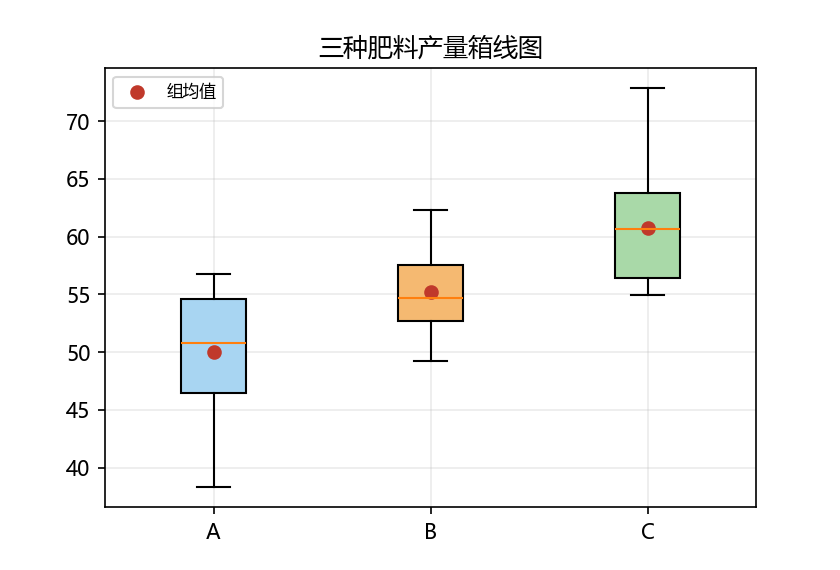
\includegraphics[keepaspectratio,alt={三种肥料的产量箱线图}]{figures/07-statsmodels/case1_fertilizer_anova.png}}
\caption{三种肥料的产量箱线图}
\end{figure}

\subsubsection{主要用法 / API}\label{ux4e3bux8981ux7528ux6cd5-api-28}

{\def\LTcaptype{none} % do not increment counter
\begin{longtable}[]{@{}
  >{\raggedright\arraybackslash}p{(\linewidth - 4\tabcolsep) * \real{0.3333}}
  >{\raggedright\arraybackslash}p{(\linewidth - 4\tabcolsep) * \real{0.3333}}
  >{\raggedright\arraybackslash}p{(\linewidth - 4\tabcolsep) * \real{0.3333}}@{}}
\toprule\noalign{}
\begin{minipage}[b]{\linewidth}\raggedright
需求
\end{minipage} & \begin{minipage}[b]{\linewidth}\raggedright
写法
\end{minipage} & \begin{minipage}[b]{\linewidth}\raggedright
说明
\end{minipage} \\
\midrule\noalign{}
\endhead
\bottomrule\noalign{}
\endlastfoot
生成正态随机数 & \texttt{rng.normal(mean,\ std,\ n)} & 模拟每组产量 \\
按组求均值 &
\texttt{df.groupby(\textquotesingle{}fertilizer\textquotesingle{}){[}\textquotesingle{}out\textquotesingle{}{]}.mean()}
& 组间比较第一步 \\
分类变量进公式 &
\texttt{ols(\textquotesingle{}out\ \textasciitilde{}\ C(fertilizer)\textquotesingle{},\ data=df)}
& \texttt{C()} 把类别变哑变量 \\
方差分析表 & \texttt{sm.stats.anova\_lm(model,\ typ=1)} & 输出
df/平方和/F/P \\
取 F / P 值 &
\texttt{anova{[}\textquotesingle{}F\textquotesingle{}{]}.iloc{[}0{]}} /
\texttt{anova{[}\textquotesingle{}PR(\textgreater{}F)\textquotesingle{}{]}.iloc{[}0{]}}
& 用 \texttt{.iloc{[}0{]}} 避免位置弃用警告 \\
画箱线图 & \texttt{plt.boxplot({[}a,\ b,\ c{]},\ tick\_labels=...)} &
直观展示组分布与均值 \\
\end{longtable}
}

\subsubsection{常见错误}\label{ux5e38ux89c1ux9519ux8bef-28}

\begin{enumerate}
\def\labelenumi{\arabic{enumi}.}
\tightlist
\item
  误把``组均值看起来不同''当成``显著不同''：还要看组内波动（\texttt{SS\_within}）够不够小；组内波动大时，均值差异可能不显著。
\item
  公式里直接写
  \texttt{ols(\textquotesingle{}out\ \textasciitilde{}\ fertilizer\textquotesingle{},\ ...)}
  而不加 \texttt{C()}：字符串列会被 patsy 当连续变量或报错。
\item
  直接用
  \texttt{anova{[}\textquotesingle{}F\textquotesingle{}{]}{[}0{]}}
  取第一行：新版 pandas 可能给出``按位置取数''的 FutureWarning，应改用
  \texttt{.iloc{[}0{]}}。
\item
  忘记在绘图前
  \texttt{os.makedirs(\textquotesingle{}images\textquotesingle{},\ exist\_ok=True)}：首次没有
  \texttt{figures/07-statsmodels/} 目录时 \texttt{savefig} 会报错。
\end{enumerate}

\subsubsection{拓展 / 跟练}\label{ux62d3ux5c55-ux8ddfux7ec3-16}

\begin{enumerate}
\def\labelenumi{\arabic{enumi}.}
\tightlist
\item
  把 \texttt{n} 改成 30，观察 F 与 P
  值如何变化；把种子改成别的值，多次运行看结论是否稳定。
\item
  用 \texttt{scipy.stats.f\_oneway(a,\ b,\ c)} 直接计算，和
  \texttt{anova\_lm} 的 F/P 对比是否一致。
\item
  给数据再加一个``对照''组（不施肥、均值 45），看 4 组 ANOVA 结论。
\item
  用 \texttt{statsmodels.stats.multicomp.pairwise\_tukeyhsd} 做 Tukey
  事后两两比较，找出哪两组差异显著。
\end{enumerate}

\begin{center}\rule{0.5\linewidth}{0.5pt}\end{center}

\subsection{2 线性回归（OLS）}\label{ux7ebfux6027ux56deux5f52ols}

\subsubsection{2.1
数组接口：sm.OLS}\label{ux6570ux7ec4ux63a5ux53e3sm.ols}

数组接口要求手动加截距列（add\_constant），适合已用 NumPy
准备数据的场景。

\begin{Shaded}
\begin{Highlighting}[]
\ImportTok{import}\NormalTok{ numpy }\ImportTok{as}\NormalTok{ np}
\ImportTok{import}\NormalTok{ statsmodels.api }\ImportTok{as}\NormalTok{ sm}

\NormalTok{rng }\OperatorTok{=}\NormalTok{ np.random.default\_rng(}\DecValTok{0}\NormalTok{)}
\NormalTok{x }\OperatorTok{=}\NormalTok{ np.linspace(}\DecValTok{0}\NormalTok{, }\DecValTok{10}\NormalTok{, }\DecValTok{50}\NormalTok{)}
\NormalTok{y }\OperatorTok{=} \DecValTok{2}\OperatorTok{*}\NormalTok{x }\OperatorTok{+} \DecValTok{1} \OperatorTok{+}\NormalTok{ rng.normal(}\DecValTok{0}\NormalTok{, }\DecValTok{1}\NormalTok{, size}\OperatorTok{=}\BuiltInTok{len}\NormalTok{(x))}

\NormalTok{X }\OperatorTok{=}\NormalTok{ sm.add\_constant(x.reshape(}\OperatorTok{{-}}\DecValTok{1}\NormalTok{, }\DecValTok{1}\NormalTok{))}
\NormalTok{model }\OperatorTok{=}\NormalTok{ sm.OLS(y, X).fit()}
\BuiltInTok{print}\NormalTok{(}\StringTok{"params:"}\NormalTok{, model.params)}
\BuiltInTok{print}\NormalTok{(}\StringTok{"R²:"}\NormalTok{, model.rsquared)}
\BuiltInTok{print}\NormalTok{(model.summary())}
\end{Highlighting}
\end{Shaded}

运行结果（Date/Time 随运行时间变化）：

\begin{Shaded}
\begin{Highlighting}[]
\NormalTok{params: [0.54884546 2.1160302 ]}
\NormalTok{R²: 0.9819621414581136}

\NormalTok{                            OLS Regression Results}
\NormalTok{==============================================================================}
\NormalTok{Dep. Variable:                      y   R{-}squared:                       0.982}
\NormalTok{Model:                            OLS   Adj. R{-}squared:                  0.982}
\NormalTok{Method:                 Least Squares   F{-}statistic:                     2613.}
\NormalTok{Date:                Wed, 26 Aug 2026   Prob (F{-}statistic):           1.63e{-}43}
\NormalTok{Time:                        14:08:23   Log{-}Likelihood:                {-}62.504}
\NormalTok{No. Observations:                  50   AIC:                             129.0}
\NormalTok{Df Residuals:                      48   BIC:                             132.8}
\NormalTok{Df Model:                           1}
\NormalTok{Covariance Type:            nonrobust}
\NormalTok{==============================================================================}
\NormalTok{                 coef    std err          t      P\textgreater{}|t|      [0.025      0.975]}
\NormalTok{{-}{-}{-}{-}{-}{-}{-}{-}{-}{-}{-}{-}{-}{-}{-}{-}{-}{-}{-}{-}{-}{-}{-}{-}{-}{-}{-}{-}{-}{-}{-}{-}{-}{-}{-}{-}{-}{-}{-}{-}{-}{-}{-}{-}{-}{-}{-}{-}{-}{-}{-}{-}{-}{-}{-}{-}{-}{-}{-}{-}{-}{-}{-}{-}{-}{-}{-}{-}{-}{-}{-}{-}{-}{-}{-}{-}{-}{-}}
\NormalTok{const          0.5488      0.240      2.285      0.027       0.066       1.032}
\NormalTok{x1             2.1160      0.041     51.118      0.000       2.033       2.199}
\NormalTok{==============================================================================}
\NormalTok{Omnibus:                        0.794   Durbin{-}Watson:                   1.565}
\NormalTok{Prob(Omnibus):                  0.672   Jarque{-}Bera (JB):                0.889}
\NormalTok{Skew:                          {-}0.229   Prob(JB):                        0.641}
\NormalTok{Kurtosis:                       2.533   Cond. No.                         11.7}
\NormalTok{==============================================================================}

\NormalTok{Notes:}
\NormalTok{[1] Standard Errors assume that the covariance matrix of the errors is correctly specified.}
\end{Highlighting}
\end{Shaded}

\begin{figure}
\centering
\pandocbounded{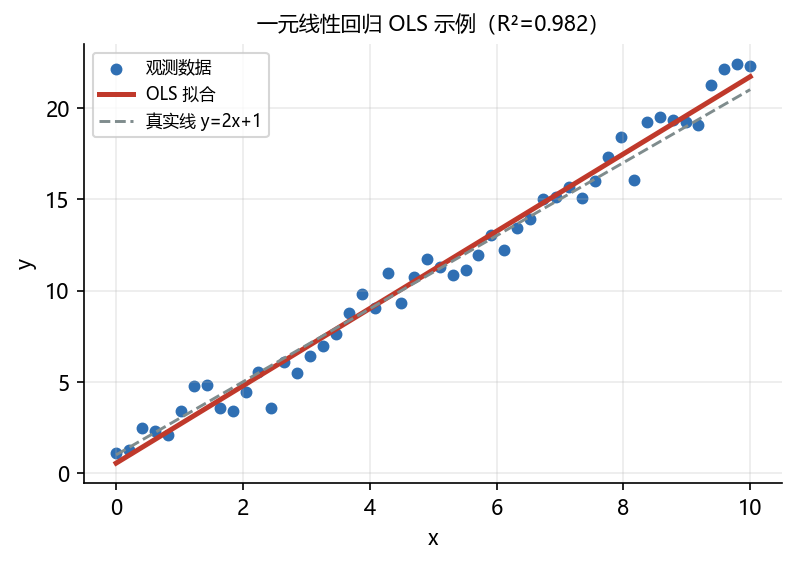
\includegraphics[keepaspectratio,alt={OLS 拟合示意}]{figures/07-statsmodels/regression_ols.png}}
\caption{OLS 拟合示意}
\end{figure}

\textbf{解读要点}：

\begin{itemize}
\tightlist
\item
  截距 const ≈ 0.549，斜率 x1 ≈ 2.116，接近真实值 \((1, 2)\)；
\item
  R²=0.982：模型解释了约 98.2\% 的方差；Adj. R² 对自变量个数做了惩罚；
\item
  F-statistic 与 Prob(F) 是整体显著性检验；Prob(F) ≈
  1.6e-43，模型整体显著；
\item
  每个系数的 P\textgreater\textbar t\textbar{} 是该变量是否显著（0.05
  为常用阈值）；
\item
  {[}0.025, 0.975{]} 是 95\% 置信区间。
\end{itemize}

\subsubsection{2.2 公式接口：ols}\label{ux516cux5f0fux63a5ux53e3ols}

把数据放进 DataFrame，即可用公式写模型：

\begin{Shaded}
\begin{Highlighting}[]
\ImportTok{import}\NormalTok{ pandas }\ImportTok{as}\NormalTok{ pd}
\ImportTok{from}\NormalTok{ statsmodels.formula.api }\ImportTok{import}\NormalTok{ ols}

\NormalTok{x }\OperatorTok{=}\NormalTok{ np.linspace(}\DecValTok{0}\NormalTok{, }\DecValTok{10}\NormalTok{, }\DecValTok{50}\NormalTok{)}
\NormalTok{y }\OperatorTok{=} \DecValTok{2}\OperatorTok{*}\NormalTok{x }\OperatorTok{+} \DecValTok{1} \OperatorTok{+}\NormalTok{ rng.normal(}\DecValTok{0}\NormalTok{, }\DecValTok{1}\NormalTok{, size}\OperatorTok{=}\BuiltInTok{len}\NormalTok{(x))}
\NormalTok{df2 }\OperatorTok{=}\NormalTok{ pd.DataFrame(\{}\StringTok{\textquotesingle{}x\textquotesingle{}}\NormalTok{: x, }\StringTok{\textquotesingle{}y\textquotesingle{}}\NormalTok{: y\})}
\NormalTok{fm }\OperatorTok{=}\NormalTok{ ols(}\StringTok{\textquotesingle{}y \textasciitilde{} x\textquotesingle{}}\NormalTok{, data}\OperatorTok{=}\NormalTok{df2).fit()}
\BuiltInTok{print}\NormalTok{(fm.params)}
\BuiltInTok{print}\NormalTok{(fm.summary())}
\end{Highlighting}
\end{Shaded}

运行结果：

\begin{Shaded}
\begin{Highlighting}[]
\NormalTok{Intercept    0.548845}
\NormalTok{x            2.116030}
\NormalTok{dtype: float64}
\end{Highlighting}
\end{Shaded}

可见公式接口默认加截距（Intercept），且列名直接用 x。其余统计量与 2.1
完全一致。

\subsubsection{2.3 多元回归}\label{ux591aux5143ux56deux5f52}

\begin{Shaded}
\begin{Highlighting}[]
\NormalTok{rng }\OperatorTok{=}\NormalTok{ np.random.default\_rng(}\DecValTok{2}\NormalTok{)}
\NormalTok{x1 }\OperatorTok{=}\NormalTok{ rng.uniform(}\DecValTok{0}\NormalTok{, }\DecValTok{10}\NormalTok{, }\DecValTok{60}\NormalTok{)}
\NormalTok{x2 }\OperatorTok{=}\NormalTok{ rng.uniform(}\OperatorTok{{-}}\DecValTok{3}\NormalTok{, }\DecValTok{3}\NormalTok{, }\DecValTok{60}\NormalTok{)}
\NormalTok{y2 }\OperatorTok{=} \DecValTok{1} \OperatorTok{+} \DecValTok{2}\OperatorTok{*}\NormalTok{x1 }\OperatorTok{{-}} \DecValTok{3}\OperatorTok{*}\NormalTok{x2 }\OperatorTok{+}\NormalTok{ rng.normal(}\DecValTok{0}\NormalTok{, }\DecValTok{1}\NormalTok{, }\DecValTok{60}\NormalTok{)}
\NormalTok{dm }\OperatorTok{=}\NormalTok{ pd.DataFrame(\{}\StringTok{\textquotesingle{}x1\textquotesingle{}}\NormalTok{: x1, }\StringTok{\textquotesingle{}x2\textquotesingle{}}\NormalTok{: x2, }\StringTok{\textquotesingle{}y\textquotesingle{}}\NormalTok{: y2\})}
\NormalTok{mul }\OperatorTok{=}\NormalTok{ ols(}\StringTok{\textquotesingle{}y \textasciitilde{} x1 + x2\textquotesingle{}}\NormalTok{, data}\OperatorTok{=}\NormalTok{dm).fit()}
\BuiltInTok{print}\NormalTok{(mul.params)}
\BuiltInTok{print}\NormalTok{(mul.pvalues)}
\BuiltInTok{print}\NormalTok{(}\StringTok{"R² ="}\NormalTok{, mul.rsquared)}
\end{Highlighting}
\end{Shaded}

运行结果：

\begin{Shaded}
\begin{Highlighting}[]
\NormalTok{Intercept    0.938724}
\NormalTok{x1           1.994930}
\NormalTok{x2          {-}3.056829}
\NormalTok{dtype: float64}
\NormalTok{Intercept    4.204720e{-}04}
\NormalTok{x1           3.299329e{-}47}
\NormalTok{x2           4.863608e{-}49}
\NormalTok{dtype: float64}
\NormalTok{R² = 0.9867366706540099}
\end{Highlighting}
\end{Shaded}

说明：两个自变量的 P 值都远小于 0.05，均显著；系数接近真实值
\((2, -3)\)。

\subsubsection{2.4
公式写法小结}\label{ux516cux5f0fux5199ux6cd5ux5c0fux7ed3}

{\def\LTcaptype{none} % do not increment counter
\begin{longtable}[]{@{}ll@{}}
\toprule\noalign{}
写法 & 含义 \\
\midrule\noalign{}
\endhead
\bottomrule\noalign{}
\endlastfoot
y \textasciitilde{} x & 一元线性 \\
y \textasciitilde{} x1 + x2 & 多元线性（可加性） \\
y \textasciitilde{} C(group) & 把 group 当分类变量（用于 ANOVA） \\
y \textasciitilde{} x1 * x2 & 主效应 + 交互项 \\
y \textasciitilde{} x1 + I(x1**2) & 添加二次项 \\
\end{longtable}
}

\subsection{案例卡 2：OLS 多元回归------用公式接口解读系数与 p
值}\label{ux6848ux4f8bux5361-2ols-ux591aux5143ux56deux5f52ux7528ux516cux5f0fux63a5ux53e3ux89e3ux8bfbux7cfbux6570ux4e0e-p-ux503c}

\subsubsection{目标}\label{ux76eeux6807-28}

造一份``房子面积（平方米）、房龄（年）→
房价（万元）''的模拟数据，用\textbf{公式接口}
\texttt{ols(\textquotesingle{}price\ \textasciitilde{}\ area\ +\ age\textquotesingle{},\ data=df)}
一次估计两个自变量。我们重点关注每个系数的\textbf{大小、符号、p 值、95\%
置信区间}，并说明``面积每大一平米、房龄每多一年，房价平均怎么变''。

\subsubsection{代码}\label{ux4ee3ux7801-29}

\begin{Shaded}
\begin{Highlighting}[]
\ImportTok{import}\NormalTok{ numpy }\ImportTok{as}\NormalTok{ np}
\ImportTok{import}\NormalTok{ pandas }\ImportTok{as}\NormalTok{ pd}
\ImportTok{from}\NormalTok{ statsmodels.formula.api }\ImportTok{import}\NormalTok{ ols}
\ImportTok{import}\NormalTok{ matplotlib.pyplot }\ImportTok{as}\NormalTok{ plt}
\ImportTok{import}\NormalTok{ os}

\NormalTok{plt.rcParams[}\StringTok{\textquotesingle{}font.sans{-}serif\textquotesingle{}}\NormalTok{] }\OperatorTok{=}\NormalTok{ [}\StringTok{\textquotesingle{}Microsoft YaHei\textquotesingle{}}\NormalTok{, }\StringTok{\textquotesingle{}SimHei\textquotesingle{}}\NormalTok{, }\StringTok{\textquotesingle{}DejaVu Sans\textquotesingle{}}\NormalTok{]}
\NormalTok{plt.rcParams[}\StringTok{\textquotesingle{}axes.unicode\_minus\textquotesingle{}}\NormalTok{] }\OperatorTok{=} \VariableTok{False}
\NormalTok{np.set\_printoptions(precision}\OperatorTok{=}\DecValTok{4}\NormalTok{, suppress}\OperatorTok{=}\VariableTok{True}\NormalTok{)}
\NormalTok{pd.set\_option(}\StringTok{\textquotesingle{}display.width\textquotesingle{}}\NormalTok{, }\DecValTok{100}\NormalTok{)}

\NormalTok{rng }\OperatorTok{=}\NormalTok{ np.random.default\_rng(}\DecValTok{3}\NormalTok{)}
\NormalTok{n }\OperatorTok{=} \DecValTok{40}
\NormalTok{area }\OperatorTok{=}\NormalTok{ rng.uniform(}\DecValTok{30}\NormalTok{, }\DecValTok{120}\NormalTok{, n)    }\CommentTok{\# 面积：30\textasciitilde{}120 平米}
\NormalTok{age }\OperatorTok{=}\NormalTok{ rng.uniform(}\DecValTok{0}\NormalTok{, }\DecValTok{30}\NormalTok{, n)       }\CommentTok{\# 房龄：0\textasciitilde{}30 年}
\NormalTok{price }\OperatorTok{=} \DecValTok{50} \OperatorTok{+} \FloatTok{3.0}\OperatorTok{*}\NormalTok{area }\OperatorTok{{-}} \FloatTok{1.5}\OperatorTok{*}\NormalTok{age }\OperatorTok{+}\NormalTok{ rng.normal(}\DecValTok{0}\NormalTok{, }\DecValTok{8}\NormalTok{, n)  }\CommentTok{\# 真实模型}

\NormalTok{df }\OperatorTok{=}\NormalTok{ pd.DataFrame(\{}\StringTok{\textquotesingle{}area\textquotesingle{}}\NormalTok{: area, }\StringTok{\textquotesingle{}age\textquotesingle{}}\NormalTok{: age, }\StringTok{\textquotesingle{}price\textquotesingle{}}\NormalTok{: price\})}
\NormalTok{model }\OperatorTok{=}\NormalTok{ ols(}\StringTok{\textquotesingle{}price \textasciitilde{} area + age\textquotesingle{}}\NormalTok{, data}\OperatorTok{=}\NormalTok{df).fit()}
\NormalTok{ci }\OperatorTok{=}\NormalTok{ model.conf\_int()}

\BuiltInTok{print}\NormalTok{(}\StringTok{\textquotesingle{}coefficients:\textquotesingle{}}\NormalTok{)}
\ControlFlowTok{for}\NormalTok{ name }\KeywordTok{in}\NormalTok{ [}\StringTok{\textquotesingle{}Intercept\textquotesingle{}}\NormalTok{, }\StringTok{\textquotesingle{}area\textquotesingle{}}\NormalTok{, }\StringTok{\textquotesingle{}age\textquotesingle{}}\NormalTok{]:}
    \BuiltInTok{print}\NormalTok{(}\SpecialStringTok{f"}\SpecialCharTok{\{}\NormalTok{name}\SpecialCharTok{:9s\}}\SpecialStringTok{ coef=}\SpecialCharTok{\{}\NormalTok{model}\SpecialCharTok{.}\NormalTok{params[name]}\SpecialCharTok{:.4f\}}\SpecialStringTok{ p=}\SpecialCharTok{\{}\NormalTok{model}\SpecialCharTok{.}\NormalTok{pvalues[name]}\SpecialCharTok{:.2e\}}\SpecialStringTok{ CI=[}\SpecialCharTok{\{}\NormalTok{ci}\SpecialCharTok{.}\NormalTok{loc[name,}\DecValTok{0}\NormalTok{]}\SpecialCharTok{:.4f\}}\SpecialStringTok{, }\SpecialCharTok{\{}\NormalTok{ci}\SpecialCharTok{.}\NormalTok{loc[name,}\DecValTok{1}\NormalTok{]}\SpecialCharTok{:.4f\}}\SpecialStringTok{]"}\NormalTok{)}
\BuiltInTok{print}\NormalTok{(}\StringTok{\textquotesingle{}R2 =\textquotesingle{}}\NormalTok{, }\BuiltInTok{round}\NormalTok{(model.rsquared, }\DecValTok{4}\NormalTok{))}
\BuiltInTok{print}\NormalTok{(}\StringTok{\textquotesingle{}F =\textquotesingle{}}\NormalTok{, }\BuiltInTok{round}\NormalTok{(model.fvalue, }\DecValTok{3}\NormalTok{), }\StringTok{\textquotesingle{} P(F) = }\SpecialCharTok{\%.3g}\StringTok{\textquotesingle{}} \OperatorTok{\%}\NormalTok{ model.f\_pvalue)}
\BuiltInTok{print}\NormalTok{(}\StringTok{\textquotesingle{}AIC =\textquotesingle{}}\NormalTok{, }\BuiltInTok{round}\NormalTok{(model.aic, }\DecValTok{2}\NormalTok{))}

\NormalTok{os.makedirs(}\StringTok{\textquotesingle{}images\textquotesingle{}}\NormalTok{, exist\_ok}\OperatorTok{=}\VariableTok{True}\NormalTok{)}
\NormalTok{fig, axes }\OperatorTok{=}\NormalTok{ plt.subplots(}\DecValTok{1}\NormalTok{, }\DecValTok{2}\NormalTok{, figsize}\OperatorTok{=}\NormalTok{(}\DecValTok{9}\NormalTok{, }\FloatTok{3.6}\NormalTok{))}
\NormalTok{axes[}\DecValTok{0}\NormalTok{].scatter(model.fittedvalues, df[}\StringTok{\textquotesingle{}price\textquotesingle{}}\NormalTok{], s}\OperatorTok{=}\DecValTok{16}\NormalTok{, color}\OperatorTok{=}\StringTok{\textquotesingle{}\#2f6fb3\textquotesingle{}}\NormalTok{, alpha}\OperatorTok{=}\FloatTok{0.7}\NormalTok{)}
\NormalTok{axes[}\DecValTok{0}\NormalTok{].plot([df[}\StringTok{\textquotesingle{}price\textquotesingle{}}\NormalTok{].}\BuiltInTok{min}\NormalTok{(), df[}\StringTok{\textquotesingle{}price\textquotesingle{}}\NormalTok{].}\BuiltInTok{max}\NormalTok{()], [df[}\StringTok{\textquotesingle{}price\textquotesingle{}}\NormalTok{].}\BuiltInTok{min}\NormalTok{(), df[}\StringTok{\textquotesingle{}price\textquotesingle{}}\NormalTok{].}\BuiltInTok{max}\NormalTok{()], color}\OperatorTok{=}\StringTok{\textquotesingle{}\#c0392b\textquotesingle{}}\NormalTok{, lw}\OperatorTok{=}\FloatTok{1.6}\NormalTok{)}
\NormalTok{axes[}\DecValTok{0}\NormalTok{].set\_xlabel(}\StringTok{\textquotesingle{}拟合值\textquotesingle{}}\NormalTok{)}\OperatorTok{;}\NormalTok{ axes[}\DecValTok{0}\NormalTok{].set\_ylabel(}\StringTok{\textquotesingle{}真实值\textquotesingle{}}\NormalTok{)}\OperatorTok{;}\NormalTok{ axes[}\DecValTok{0}\NormalTok{].set\_title(}\StringTok{\textquotesingle{}拟合值 vs 真实值\textquotesingle{}}\NormalTok{)}
\NormalTok{axes[}\DecValTok{1}\NormalTok{].scatter(model.fittedvalues, model.resid, s}\OperatorTok{=}\DecValTok{16}\NormalTok{, color}\OperatorTok{=}\StringTok{\textquotesingle{}\#3a8f4f\textquotesingle{}}\NormalTok{, alpha}\OperatorTok{=}\FloatTok{0.7}\NormalTok{)}
\NormalTok{axes[}\DecValTok{1}\NormalTok{].axhline(}\DecValTok{0}\NormalTok{, color}\OperatorTok{=}\StringTok{\textquotesingle{}\#c0392b\textquotesingle{}}\NormalTok{, lw}\OperatorTok{=}\FloatTok{1.2}\NormalTok{)}
\NormalTok{axes[}\DecValTok{1}\NormalTok{].set\_xlabel(}\StringTok{\textquotesingle{}拟合值\textquotesingle{}}\NormalTok{)}\OperatorTok{;}\NormalTok{ axes[}\DecValTok{1}\NormalTok{].set\_ylabel(}\StringTok{\textquotesingle{}残差\textquotesingle{}}\NormalTok{)}\OperatorTok{;}\NormalTok{ axes[}\DecValTok{1}\NormalTok{].set\_title(}\StringTok{\textquotesingle{}残差 vs 拟合值\textquotesingle{}}\NormalTok{)}
\ControlFlowTok{for}\NormalTok{ ax }\KeywordTok{in}\NormalTok{ axes:}
\NormalTok{    ax.grid(alpha}\OperatorTok{=}\FloatTok{0.25}\NormalTok{)}
\NormalTok{fig.tight\_layout()}
\NormalTok{fig.savefig(}\StringTok{\textquotesingle{}figures/07{-}statsmodels/case2\_ols\_multi.png\textquotesingle{}}\NormalTok{, dpi}\OperatorTok{=}\DecValTok{150}\NormalTok{)}
\NormalTok{plt.close()}
\BuiltInTok{print}\NormalTok{(}\StringTok{\textquotesingle{}saved figures/07{-}statsmodels/case2\_ols\_multi.png\textquotesingle{}}\NormalTok{)}
\end{Highlighting}
\end{Shaded}

\subsubsection{运行结果（已运行核验）}\label{ux8fd0ux884cux7ed3ux679cux5df2ux8fd0ux884cux6838ux9a8c-27}

\begin{Shaded}
\begin{Highlighting}[]
\NormalTok{coefficients:}
\NormalTok{Intercept coef=50.8786 p=2.16e{-}12 CI=[40.8480, 60.9092]}
\NormalTok{area      coef=2.9799 p=1.59e{-}36 CI=[2.8662, 3.0937]}
\NormalTok{age       coef={-}1.4557 p=8.11e{-}11 CI=[{-}1.7844, {-}1.1269]}
\NormalTok{R2 = 0.9872}
\NormalTok{F = 1425.282  P(F) = 9.82e{-}36}
\NormalTok{AIC = 290.09}
\NormalTok{saved figures/07{-}statsmodels/case2\_ols\_multi.png}
\end{Highlighting}
\end{Shaded}

\subsubsection{讲解}\label{ux8bb2ux89e3-27}

\textbf{一句话解释}：房价 ≈ 一个``起步价'' + 每平米单价 × 面积 −
每年折旧 × 房龄；\texttt{coef} 就是这些单价，\texttt{p}
告诉你``这个单价是不是真的、会不会只是噪声''。

\begin{enumerate}
\def\labelenumi{\arabic{enumi}.}
\tightlist
\item
  \texttt{area\ =\ rng.uniform(30,\ 120,\ n)}：生成 40
  套房子的面积；\texttt{age} 类似。\texttt{price} 用真实系数
  \texttt{(50,\ 3,\ -1.5)}
  再加噪声构造，这样我们能``对着答案''检验模型。
\item
  \texttt{ols(\textquotesingle{}price\ \textasciitilde{}\ area\ +\ age\textquotesingle{},\ data=df)}：公式接口自动加截距（\texttt{Intercept}），并同时放进
  \texttt{area} 与 \texttt{age} 两个自变量。
\item
  \texttt{model.params}：截距 ≈50.88（接近真实 50），\texttt{area}
  ≈2.98（接近真实 3），\texttt{age} ≈−1.46（接近真实
  −1.5）。系数就是``在控制另一个变量后，该变量每改变 1
  单位，因变量的平均变化''。
\item
  \texttt{model.pvalues}：三个 p 值都远小于
  0.05，说明截距、面积、房龄都\textbf{统计显著}；房龄系数为负也符合直觉（房子越旧越便宜）。
\item
  \texttt{model.conf\_int()}：给出 95\% 置信区间。\texttt{area} 的区间
  \texttt{{[}2.87,\ 3.09{]}} 不包含
  0，说明面积效应显著为正；\texttt{age} 区间
  \texttt{{[}-1.78,\ -1.13{]}} 不包含 0，说明房龄效应显著为负。
\item
  \texttt{R2=0.9872}：面积+房龄解释了约 98.7\% 的房价变动；\texttt{F} 与
  \texttt{p(F)} 说明模型整体显著。\texttt{AIC} 可用于与其它模型比较。
\end{enumerate}

\begin{figure}
\centering
\pandocbounded{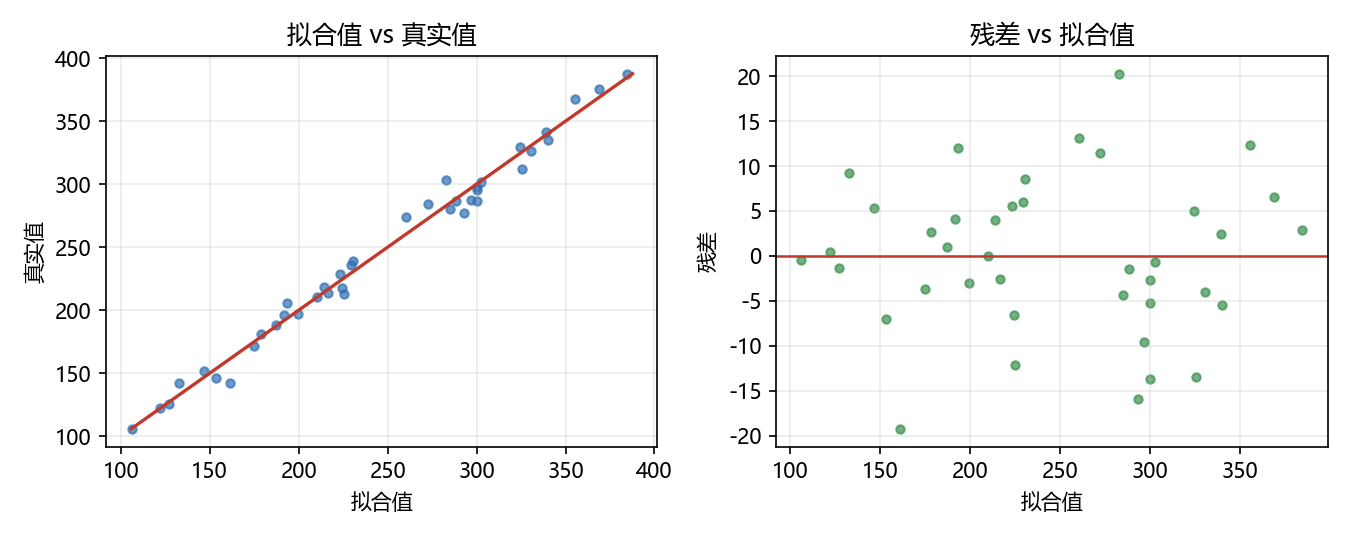
\includegraphics[keepaspectratio,alt={拟合值 vs 真实值 与 残差图}]{figures/07-statsmodels/case2_ols_multi.png}}
\caption{拟合值 vs 真实值 与 残差图}
\end{figure}

\subsubsection{主要用法 / API}\label{ux4e3bux8981ux7528ux6cd5-api-29}

{\def\LTcaptype{none} % do not increment counter
\begin{longtable}[]{@{}
  >{\raggedright\arraybackslash}p{(\linewidth - 4\tabcolsep) * \real{0.3333}}
  >{\raggedright\arraybackslash}p{(\linewidth - 4\tabcolsep) * \real{0.3333}}
  >{\raggedright\arraybackslash}p{(\linewidth - 4\tabcolsep) * \real{0.3333}}@{}}
\toprule\noalign{}
\begin{minipage}[b]{\linewidth}\raggedright
需求
\end{minipage} & \begin{minipage}[b]{\linewidth}\raggedright
写法
\end{minipage} & \begin{minipage}[b]{\linewidth}\raggedright
说明
\end{minipage} \\
\midrule\noalign{}
\endhead
\bottomrule\noalign{}
\endlastfoot
多元回归 &
\texttt{ols(\textquotesingle{}price\ \textasciitilde{}\ area\ +\ age\textquotesingle{},\ data=df)}
& 公式接口，自动加截距 \\
系数 & \texttt{model.params} & 每个变量的边际效应 \\
p 值 & \texttt{model.pvalues} & \textless0.05 视为显著 \\
置信区间 & \texttt{model.conf\_int()} & 95\% CI，不含 0 一般显著 \\
拟合优度 & \texttt{model.rsquared} / \texttt{model.rsquared\_adj} &
解释比例 / 调整后 \\
整体显著性 & \texttt{model.fvalue} / \texttt{model.f\_pvalue} &
所有系数联合是否为 0 \\
信息准则 & \texttt{model.aic} & 越小越好，用于模型选择 \\
\end{longtable}
}

\subsubsection{常见错误}\label{ux5e38ux89c1ux9519ux8bef-29}

\begin{enumerate}
\def\labelenumi{\arabic{enumi}.}
\tightlist
\item
  只打印 \texttt{model.summary()}
  而不使用关键字段：跨版本摘要边缘（空格、分隔线、\texttt{+/-}
  号）不稳定，教学时建议用
  \texttt{params}/\texttt{pvalues}/\texttt{conf\_int} 打印固定字段。
\item
  忘记 \texttt{add\_constant}
  但用了数组接口：公式接口自动加截距，数组接口却要手动加。
\item
  把 \texttt{p=0.0} 直接打印当``无意义''：应使用 \texttt{\%.2e} 或
  \texttt{\%.3g} 科学计数法，避免显示成 0。
\item
  用 \texttt{round(model.pvalues,\ 4)} 输出时 p 值太小被四舍五入成
  0.0000，看不出数量级。
\end{enumerate}

\subsubsection{拓展 / 跟练}\label{ux62d3ux5c55-ux8ddfux7ec3-17}

\begin{enumerate}
\def\labelenumi{\arabic{enumi}.}
\tightlist
\item
  在公式里加交互项
  \texttt{ols(\textquotesingle{}price\ \textasciitilde{}\ area\ +\ age\ +\ area:age\textquotesingle{},\ data=df)}，看交互项是否显著。
\item
  把 \texttt{age} 换成``新房/二手''分类变量
  \texttt{C(new\_house)}，对比系数含义变化。
\item
  用数组接口
  \texttt{sm.OLS(df{[}\textquotesingle{}price\textquotesingle{}{]},\ sm.add\_constant(df{[}{[}\textquotesingle{}area\textquotesingle{},\textquotesingle{}age\textquotesingle{}{]}{]}))}
  重跑，确认系数一致。
\item
  计算各自变量的标准化系数（\texttt{z-score}
  后回归），比较``谁的影响更大''。
\end{enumerate}

\begin{center}\rule{0.5\linewidth}{0.5pt}\end{center}

\subsection{3 回归诊断：残差 QQ 图与 JB
统计量}\label{ux56deux5f52ux8bcaux65adux6b8bux5dee-qq-ux56feux4e0e-jb-ux7edfux8ba1ux91cf}

\subsubsection{3.1 为什么诊断}\label{ux4e3aux4ec0ux4e48ux8bcaux65ad}

OLS 的统计推断（t/F/P
值）依赖于\textbf{误差项独立同分布、同方差、近似正态}。诊断残差是否偏离这些假设，能及时发现模型设定问题。

\begin{Shaded}
\begin{Highlighting}[]
\ImportTok{import}\NormalTok{ matplotlib.pyplot }\ImportTok{as}\NormalTok{ plt}
\NormalTok{rng }\OperatorTok{=}\NormalTok{ np.random.default\_rng(}\DecValTok{0}\NormalTok{)}
\NormalTok{xd }\OperatorTok{=}\NormalTok{ np.linspace(}\DecValTok{0}\NormalTok{, }\DecValTok{10}\NormalTok{, }\DecValTok{50}\NormalTok{)}
\NormalTok{yd }\OperatorTok{=} \DecValTok{3}\OperatorTok{*}\NormalTok{xd }\OperatorTok{+} \DecValTok{2} \OperatorTok{+}\NormalTok{ rng.normal(}\DecValTok{0}\NormalTok{, }\DecValTok{1}\NormalTok{, }\DecValTok{50}\NormalTok{)}
\NormalTok{Xd }\OperatorTok{=}\NormalTok{ sm.add\_constant(xd.reshape(}\OperatorTok{{-}}\DecValTok{1}\NormalTok{, }\DecValTok{1}\NormalTok{))}
\NormalTok{olsd }\OperatorTok{=}\NormalTok{ sm.OLS(yd, Xd).fit()}
\NormalTok{sm.qqplot(olsd.resid, line}\OperatorTok{=}\StringTok{\textquotesingle{}45\textquotesingle{}}\NormalTok{)}
\NormalTok{plt.title(}\StringTok{"残差 QQ 图"}\NormalTok{)}
\NormalTok{plt.show()}
\BuiltInTok{print}\NormalTok{(olsd.summary())}
\end{Highlighting}
\end{Shaded}

在模型摘要中可找到：

\begin{Shaded}
\begin{Highlighting}[]
\NormalTok{Prob(Omnibus):                  0.672   Jarque{-}Bera (JB):                0.889}
\NormalTok{Skew:                          {-}0.229   Prob(JB):                        0.641}
\end{Highlighting}
\end{Shaded}

\begin{figure}
\centering
\pandocbounded{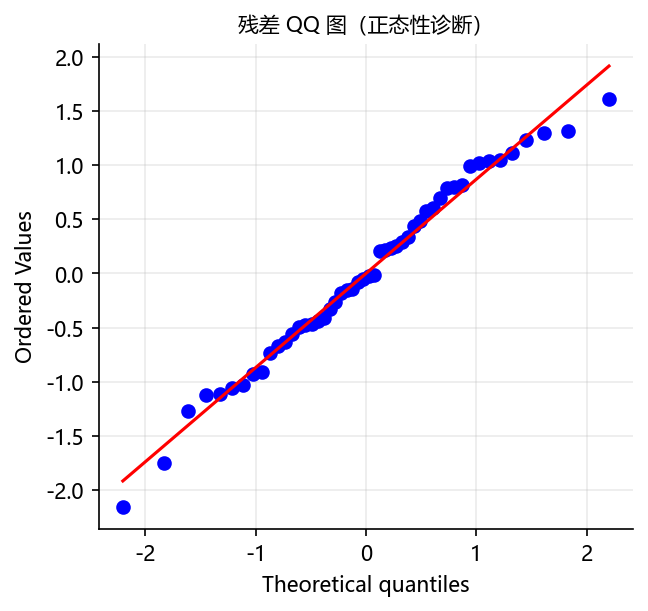
\includegraphics[keepaspectratio,alt={残差 QQ 图}]{figures/07-statsmodels/qq_resid.png}}
\caption{残差 QQ 图}
\end{figure}

\textbf{解读}：

\begin{itemize}
\tightlist
\item
  Jarque-Bera (JB) 检验残差是否为正态分布；Prob(JB)=0.641 \textgreater{}
  0.05，不能拒绝正态假设，说明残差近似正态；
\item
  QQ 图中点应落在 45° 直线附近；本例散点基本沿直线，正态性可接受。
\end{itemize}

\begin{center}\rule{0.5\linewidth}{0.5pt}\end{center}

\subsection{4
广义线性模型（GLM）}\label{ux5e7fux4e49ux7ebfux6027ux6a21ux578bglm}

\subsubsection{4.1 概念}\label{ux6982ux5ff5-1}

当因变量是\textbf{二分类}（成功/失败）、计数或比例时，OLS
不再合适。广义线性模型通过\textbf{链接函数}把线性预测值映射到合理的取值区间，并用指数族分布建模。二分类最常用
Binomial 家族 + Logit 链接（即逻辑回归）：

\[
\text{logit}(p) = \beta_0 + \beta_1 x_1 + \beta_2 x_2,\qquad
p = \frac{1}{1+e^{-(\beta_0+\beta_1 x_1+\beta_2 x_2)}}
\]

\subsubsection{4.2 二分类 Logit
示例}\label{ux4e8cux5206ux7c7b-logit-ux793aux4f8b}

\begin{Shaded}
\begin{Highlighting}[]
\ImportTok{import}\NormalTok{ numpy }\ImportTok{as}\NormalTok{ np}
\ImportTok{import}\NormalTok{ statsmodels.api }\ImportTok{as}\NormalTok{ sm}

\NormalTok{rng }\OperatorTok{=}\NormalTok{ np.random.default\_rng(}\DecValTok{0}\NormalTok{)}
\NormalTok{X\_raw }\OperatorTok{=}\NormalTok{ rng.uniform(}\DecValTok{0}\NormalTok{, }\DecValTok{1}\NormalTok{, (}\DecValTok{200}\NormalTok{, }\DecValTok{2}\NormalTok{))}
\NormalTok{lin }\OperatorTok{=} \FloatTok{0.5} \OperatorTok{+} \FloatTok{1.2}\OperatorTok{*}\NormalTok{X\_raw[:, }\DecValTok{0}\NormalTok{] }\OperatorTok{{-}} \FloatTok{0.8}\OperatorTok{*}\NormalTok{X\_raw[:, }\DecValTok{1}\NormalTok{]}
\NormalTok{p }\OperatorTok{=} \DecValTok{1}\OperatorTok{/}\NormalTok{(}\DecValTok{1}\OperatorTok{+}\NormalTok{np.exp(}\OperatorTok{{-}}\NormalTok{lin))}
\NormalTok{Y }\OperatorTok{=}\NormalTok{ rng.binomial(}\DecValTok{1}\NormalTok{, p)               }\CommentTok{\# 真实概率 p 下的二分类结果}

\NormalTok{X }\OperatorTok{=}\NormalTok{ sm.add\_constant(X\_raw)}
\NormalTok{glm }\OperatorTok{=}\NormalTok{ sm.GLM(Y, X, family}\OperatorTok{=}\NormalTok{sm.families.Binomial()).fit()}
\BuiltInTok{print}\NormalTok{(glm.params)}
\NormalTok{X\_new }\OperatorTok{=}\NormalTok{ sm.add\_constant(np.array([[}\FloatTok{0.2}\NormalTok{, }\FloatTok{0.3}\NormalTok{], [}\FloatTok{0.8}\NormalTok{, }\FloatTok{0.1}\NormalTok{]]))}
\BuiltInTok{print}\NormalTok{(glm.predict(X\_new))}
\end{Highlighting}
\end{Shaded}

运行结果：

\begin{Shaded}
\begin{Highlighting}[]
\NormalTok{params: [ 0.26505589  1.42126589 {-}0.87263185]}
\NormalTok{predict: [0.57138876 0.78831616]}
\end{Highlighting}
\end{Shaded}

\textbf{解读}：

\begin{itemize}
\tightlist
\item
  估计系数接近真实值 \((0.5, 1.2, -0.8)\)，且符号正确（x1 正、x2 负）；
\item
  predict 返回的是\textbf{概率}（经过 Logit
  反变换），两个新样本的成功概率约为 0.57 与 0.79；
\item
  若想得到 0/1 分类，可再对概率设阈值（如 \textgreater0.5 判为 1），见
  04 常见误区。
\end{itemize}

\begin{center}\rule{0.5\linewidth}{0.5pt}\end{center}

\subsection{5
加权最小二乘（WLS）处理异方差}\label{ux52a0ux6743ux6700ux5c0fux4e8cux4e58wlsux5904ux7406ux5f02ux65b9ux5dee}

当误差方差随自变量变化（异方差）时，OLS
虽无偏但效率低（标准误不准）。WLS 用权重 \(w_i\)
加权残差平方和，对异方差更稳健。

\begin{Shaded}
\begin{Highlighting}[]
\ImportTok{import}\NormalTok{ numpy }\ImportTok{as}\NormalTok{ np}
\ImportTok{import}\NormalTok{ statsmodels.api }\ImportTok{as}\NormalTok{ sm}

\NormalTok{rng }\OperatorTok{=}\NormalTok{ np.random.default\_rng(}\DecValTok{1}\NormalTok{)}
\NormalTok{xw }\OperatorTok{=}\NormalTok{ np.linspace(}\FloatTok{0.1}\NormalTok{, }\DecValTok{10}\NormalTok{, }\DecValTok{200}\NormalTok{)}
\NormalTok{eps }\OperatorTok{=}\NormalTok{ rng.normal(}\DecValTok{0}\NormalTok{, xw)            }\CommentTok{\# 标准差与 x 成正比 {-}\textgreater{} 方差与 x\^{}2 成正比}
\NormalTok{yw }\OperatorTok{=} \DecValTok{3}\OperatorTok{*}\NormalTok{xw }\OperatorTok{+}\NormalTok{ eps}
\NormalTok{Xw }\OperatorTok{=}\NormalTok{ sm.add\_constant(xw.reshape(}\OperatorTok{{-}}\DecValTok{1}\NormalTok{, }\DecValTok{1}\NormalTok{))}

\NormalTok{ols\_w }\OperatorTok{=}\NormalTok{ sm.OLS(yw, Xw).fit()}
\NormalTok{wls\_w }\OperatorTok{=}\NormalTok{ sm.WLS(yw, Xw, weights}\OperatorTok{=}\DecValTok{1}\OperatorTok{/}\NormalTok{np.square(xw)).fit()}
\BuiltInTok{print}\NormalTok{(}\StringTok{"OLS:"}\NormalTok{, np.}\BuiltInTok{round}\NormalTok{(ols\_w.params, }\DecValTok{4}\NormalTok{), }\StringTok{"bse"}\NormalTok{, np.}\BuiltInTok{round}\NormalTok{(ols\_w.bse, }\DecValTok{4}\NormalTok{))}
\BuiltInTok{print}\NormalTok{(}\StringTok{"WLS:"}\NormalTok{, np.}\BuiltInTok{round}\NormalTok{(wls\_w.params, }\DecValTok{4}\NormalTok{), }\StringTok{"bse"}\NormalTok{, np.}\BuiltInTok{round}\NormalTok{(wls\_w.bse, }\DecValTok{4}\NormalTok{))}
\end{Highlighting}
\end{Shaded}

运行结果：

\begin{Shaded}
\begin{Highlighting}[]
\NormalTok{OLS: [{-}0.0422  2.9257] bse [0.833  0.1434]}
\NormalTok{WLS: [ 0.0597  2.8971] bse [0.0641 0.0727]}
\end{Highlighting}
\end{Shaded}

\textbf{解读}：

\begin{itemize}
\tightlist
\item
  两者斜率都接近真实值 3；
\item
  但 WLS 的斜率标准误（0.0727）明显小于
  OLS（0.1434），说明在已知异方差形式（\(\sigma_i \propto x_i\)）时，WLS
  估计更有效。
\end{itemize}

\begin{center}\rule{0.5\linewidth}{0.5pt}\end{center}

\subsection{6
方差分析与回归的统一框架}\label{ux65b9ux5deeux5206ux6790ux4e0eux56deux5f52ux7684ux7edfux4e00ux6846ux67b6}

线性回归与方差分析其实共享同一套\textbf{线性模型 + 最小二乘 + F
检验}逻辑：

\begin{itemize}
\tightlist
\item
  回归用连续/哑变量做\textbf{解释}；ANOVA 用分组哑变量做\textbf{比较}；
\item
  都可以写成 \(y = X\beta + \varepsilon\)，用 ols 拟合；
\item
  都能用 F 检验判断``若干系数同时为 0''的联合显著性。
\end{itemize}

因此，ANOVA
可看成\textbf{只有分类自变量}的线性回归；回归也可看成含连续+分类变量的``广义''ANOVA。这就是为什么要用
ols + anova\_lm 而不是单独的 scipy.stats.f\_oneway 来统一步骤。

\begin{center}\rule{0.5\linewidth}{0.5pt}\end{center}

\subsection{常见误区}\label{ux5e38ux89c1ux8befux533a-20}

\begin{enumerate}
\def\labelenumi{\arabic{enumi}.}
\tightlist
\item
  \textbf{忘记加截距}：数组接口必须 X =
  sm.add\_constant(X)，否则模型强制过原点。
\item
  **用 * 表示``与''\textbf{：公式里 y \textasciitilde{} x1 * x2
  是主效应+交互项，不是数值乘法；要写原生项用 I(x1}2) 且注意加
  I(\ldots)。
\item
  \textbf{分类变量直接进公式}：对字符串列，ols(`y \textasciitilde{}
  group') 会当成连续变量或报错，应写成 C(group)。
\item
  \textbf{用 predict 忘记加常数}：数组接口预测新数据也要
  sm.add\_constant(X\_new)。
\item
  \textbf{把 GLM 的 predict 当分类输出}：默认返回概率，需要阈值才能变
  0/1。
\item
  \textbf{忽略诊断}：只报 R² 不看不残差与显著性检验，容易过拟合/误设。
\end{enumerate}

\subsection{思考题}\label{ux601dux8003ux9898-22}

\begin{enumerate}
\def\labelenumi{\arabic{enumi}.}
\tightlist
\item
  为什么数组接口里 add\_constant
  必须加？如果不加，拟合结果在什么情况下仍``正确''？
\item
  anova\_lm(model, typ=1) 与 typ=3
  在单因素时结果是否相同？在多因素时为何可能不同？
\item
  给定 y \textasciitilde{} x1 + x2，若想加入 x1 与 x2
  的交互，公式应怎么写？系数个数变成几个？
\item
  为什么 GLM 不用 OLS 直接拟合二分类因变量？（提示：概率会越界、异方差）
\end{enumerate}

\subsection{动手练习（详见
lab）}\label{ux52a8ux624bux7ec3ux4e60ux8be6ux89c1-lab-14}

\begin{itemize}
\tightlist
\item
  用 sm.OLS 拟合 y = 1 + 2x 的噪声数据，打印完整 summary()；
\item
  构造三个组，画出箱线图并做单因素方差分析；
\item
  用公式 API 拟合 y \textasciitilde{} x1 + x2，说明各系数显著性；
\item
  用 GLM(Binomial) 拟合二分类数据，并在不同阈值下计算准确率与 F1。
\end{itemize}

\subsection{延伸阅读}\label{ux5ef6ux4f38ux9605ux8bfb-31}

\begin{itemize}
\tightlist
\item
  statsmodels Regressions
  官方：\href{https://www.statsmodels.org/stable/regression.html}{链接}
\item
  statsmodels GLM
  官方：\href{https://www.statsmodels.org/stable/glm.html}{链接}
\item
  残差诊断（Statsmodels
  图示）：\href{https://www.statsmodels.org/stable/examples/index.html\#regression}{链接}
\end{itemize}

\section{02 时间序列预测}\label{ux65f6ux95f4ux5e8fux5217ux9884ux6d4b}

\begin{quote}
本节对应原版 7.2 的内容，并增补目标、平稳性检验实操与思考题。
配套图：figures/07-statsmodels/decompose\_daily.png、figures/07-statsmodels/arima\_forecast.png（由
build/make\_chap7\_figures.py 生成）。
\end{quote}

\subsection{本节目标}\label{ux672cux8282ux76eeux6807-27}

\begin{itemize}
\tightlist
\item
  会用 seasonal\_decompose 把时间序列分解为趋势、季节、残差；
\item
  会用 adfuller 做单位根检验，判断序列是否平稳；
\item
  会用 ARIMA 拟合时间序列并给出未来预测；
\item
  会从 ACF/PACF 或网格搜索选择 (p, d, q) 阶数；
\item
  能画分解图与预测图，并解读结果。
\end{itemize}

\subsection{先修}\label{ux5148ux4fee-20}

\begin{itemize}
\tightlist
\item
  Pandas 时间序列索引（date\_range、Series）；本章第 01
  节的回归/统计基础。
\item
  已安装 statsmodels（见章 README）。
\end{itemize}

\subsection{官方文档/参考入口}\label{ux5b98ux65b9ux6587ux6863ux53c2ux8003ux5165ux53e3-6}

{\def\LTcaptype{none} % do not increment counter
\begin{longtable}[]{@{}
  >{\raggedright\arraybackslash}p{(\linewidth - 4\tabcolsep) * \real{0.3333}}
  >{\raggedright\arraybackslash}p{(\linewidth - 4\tabcolsep) * \real{0.3333}}
  >{\raggedright\arraybackslash}p{(\linewidth - 4\tabcolsep) * \real{0.3333}}@{}}
\toprule\noalign{}
\begin{minipage}[b]{\linewidth}\raggedright
内容
\end{minipage} & \begin{minipage}[b]{\linewidth}\raggedright
链接
\end{minipage} & \begin{minipage}[b]{\linewidth}\raggedright
说明
\end{minipage} \\
\midrule\noalign{}
\endhead
\bottomrule\noalign{}
\endlastfoot
seasonal\_decompose &
\href{https://www.statsmodels.org/stable/generated/statsmodels.tsa.seasonal.seasonal_decompose.html}{链接}
& 时间序列分解 \\
adfuller &
\href{https://www.statsmodels.org/stable/generated/statsmodels.tsa.stattools.adfuller.html}{链接}
& ADF 单位根检验 \\
ARIMA &
\href{https://www.statsmodels.org/stable/generated/statsmodels.tsa.arima.model.ARIMA.html}{链接}
& ARIMA 模型 \\
时间序列官方教程 &
\href{https://www.statsmodels.org/stable/tsa.html}{链接} &
时间序列总览 \\
\end{longtable}
}

\begin{center}\rule{0.5\linewidth}{0.5pt}\end{center}

\subsection{1
时间序列分解（seasonal\_decompose）}\label{ux65f6ux95f4ux5e8fux5217ux5206ux89e3seasonal_decompose}

\subsubsection{1.1 概念}\label{ux6982ux5ff5-2}

把序列 \(y_t\) 拆成三部分：

\[
y_t = T_t + S_t + R_t \quad(\text{加法模型})
\qquad\text{或}\qquad
y_t = T_t \times S_t \times R_t \quad(\text{乘法模型})
\]

其中 \(T_t\) 是\textbf{趋势}、\(S_t\) 是\textbf{季节}、\(R_t\)
是\textbf{残差}。加法模型适合波动幅度不随水平变化的序列；乘法模型适合幅度随水平增长的序列。

\subsubsection{1.2 日数据（周期=7
天）}\label{ux65e5ux6570ux636eux5468ux671f7-ux5929}

构造 180 天日序列：线性趋势 + 周季节性（正弦，周期 7）+ 噪声。

\begin{Shaded}
\begin{Highlighting}[]
\ImportTok{import}\NormalTok{ numpy }\ImportTok{as}\NormalTok{ np}
\ImportTok{import}\NormalTok{ pandas }\ImportTok{as}\NormalTok{ pd}
\ImportTok{import}\NormalTok{ statsmodels.api }\ImportTok{as}\NormalTok{ sm}
\ImportTok{import}\NormalTok{ matplotlib.pyplot }\ImportTok{as}\NormalTok{ plt}
\ImportTok{from}\NormalTok{ statsmodels.tsa.seasonal }\ImportTok{import}\NormalTok{ seasonal\_decompose}

\NormalTok{plt.rcParams[}\StringTok{\textquotesingle{}font.sans{-}serif\textquotesingle{}}\NormalTok{] }\OperatorTok{=}\NormalTok{ [}\StringTok{\textquotesingle{}Microsoft YaHei\textquotesingle{}}\NormalTok{, }\StringTok{\textquotesingle{}SimHei\textquotesingle{}}\NormalTok{, }\StringTok{\textquotesingle{}DejaVu Sans\textquotesingle{}}\NormalTok{]}
\NormalTok{plt.rcParams[}\StringTok{\textquotesingle{}axes.unicode\_minus\textquotesingle{}}\NormalTok{] }\OperatorTok{=} \VariableTok{False}

\NormalTok{rng }\OperatorTok{=}\NormalTok{ np.random.default\_rng(}\DecValTok{0}\NormalTok{)}
\NormalTok{idx }\OperatorTok{=}\NormalTok{ pd.date\_range(}\StringTok{\textquotesingle{}2022{-}01{-}01\textquotesingle{}}\NormalTok{, periods}\OperatorTok{=}\DecValTok{180}\NormalTok{, freq}\OperatorTok{=}\StringTok{\textquotesingle{}D\textquotesingle{}}\NormalTok{)}
\NormalTok{trend }\OperatorTok{=}\NormalTok{ np.linspace(}\DecValTok{0}\NormalTok{, }\DecValTok{5}\NormalTok{, }\BuiltInTok{len}\NormalTok{(idx))}
\NormalTok{season }\OperatorTok{=} \DecValTok{2}\OperatorTok{*}\NormalTok{np.sin(}\DecValTok{2}\OperatorTok{*}\NormalTok{np.pi}\OperatorTok{*}\NormalTok{np.arange(}\BuiltInTok{len}\NormalTok{(idx))}\OperatorTok{/}\DecValTok{7}\NormalTok{)}
\NormalTok{noise }\OperatorTok{=}\NormalTok{ rng.normal(}\DecValTok{0}\NormalTok{, }\FloatTok{0.5}\NormalTok{, }\BuiltInTok{len}\NormalTok{(idx))}
\NormalTok{s }\OperatorTok{=}\NormalTok{ pd.Series(}\DecValTok{10} \OperatorTok{+}\NormalTok{ trend }\OperatorTok{+}\NormalTok{ season }\OperatorTok{+}\NormalTok{ noise, index}\OperatorTok{=}\NormalTok{idx)}

\NormalTok{result }\OperatorTok{=}\NormalTok{ seasonal\_decompose(s, model}\OperatorTok{=}\StringTok{\textquotesingle{}additive\textquotesingle{}}\NormalTok{, period}\OperatorTok{=}\DecValTok{7}\NormalTok{)}
\BuiltInTok{print}\NormalTok{(}\StringTok{"trend head:"}\NormalTok{, np.}\BuiltInTok{round}\NormalTok{(result.trend.head(}\DecValTok{7}\NormalTok{).values, }\DecValTok{3}\NormalTok{))}
\BuiltInTok{print}\NormalTok{(}\StringTok{"seasonal head:"}\NormalTok{, np.}\BuiltInTok{round}\NormalTok{(result.seasonal.head(}\DecValTok{7}\NormalTok{).values, }\DecValTok{3}\NormalTok{))}
\BuiltInTok{print}\NormalTok{(}\StringTok{"resid describe:"}\NormalTok{, result.resid.describe().}\BuiltInTok{round}\NormalTok{(}\DecValTok{4}\NormalTok{).to\_dict())}
\NormalTok{result.plot()}
\NormalTok{plt.show()}
\end{Highlighting}
\end{Shaded}

运行结果：

\begin{Shaded}
\begin{Highlighting}[]
\NormalTok{trend head: [   nan    nan    nan 10.217 10.304 10.291 10.183]}
\NormalTok{seasonal head: [ 0.08   1.485  2.005  0.898 {-}0.765 {-}2.135 {-}1.567]}
\NormalTok{resid describe: \{\textquotesingle{}count\textquotesingle{}: 174.0, \textquotesingle{}mean\textquotesingle{}: {-}0.0018, \textquotesingle{}std\textquotesingle{}: 0.4279, \textquotesingle{}min\textquotesingle{}: {-}1.3175, \textquotesingle{}25\%\textquotesingle{}: {-}0.3194, \textquotesingle{}50\%\textquotesingle{}: 0.0279, \textquotesingle{}75\%\textquotesingle{}: 0.3018, \textquotesingle{}max\textquotesingle{}: 0.9416\}}
\end{Highlighting}
\end{Shaded}

\begin{figure}
\centering
\pandocbounded{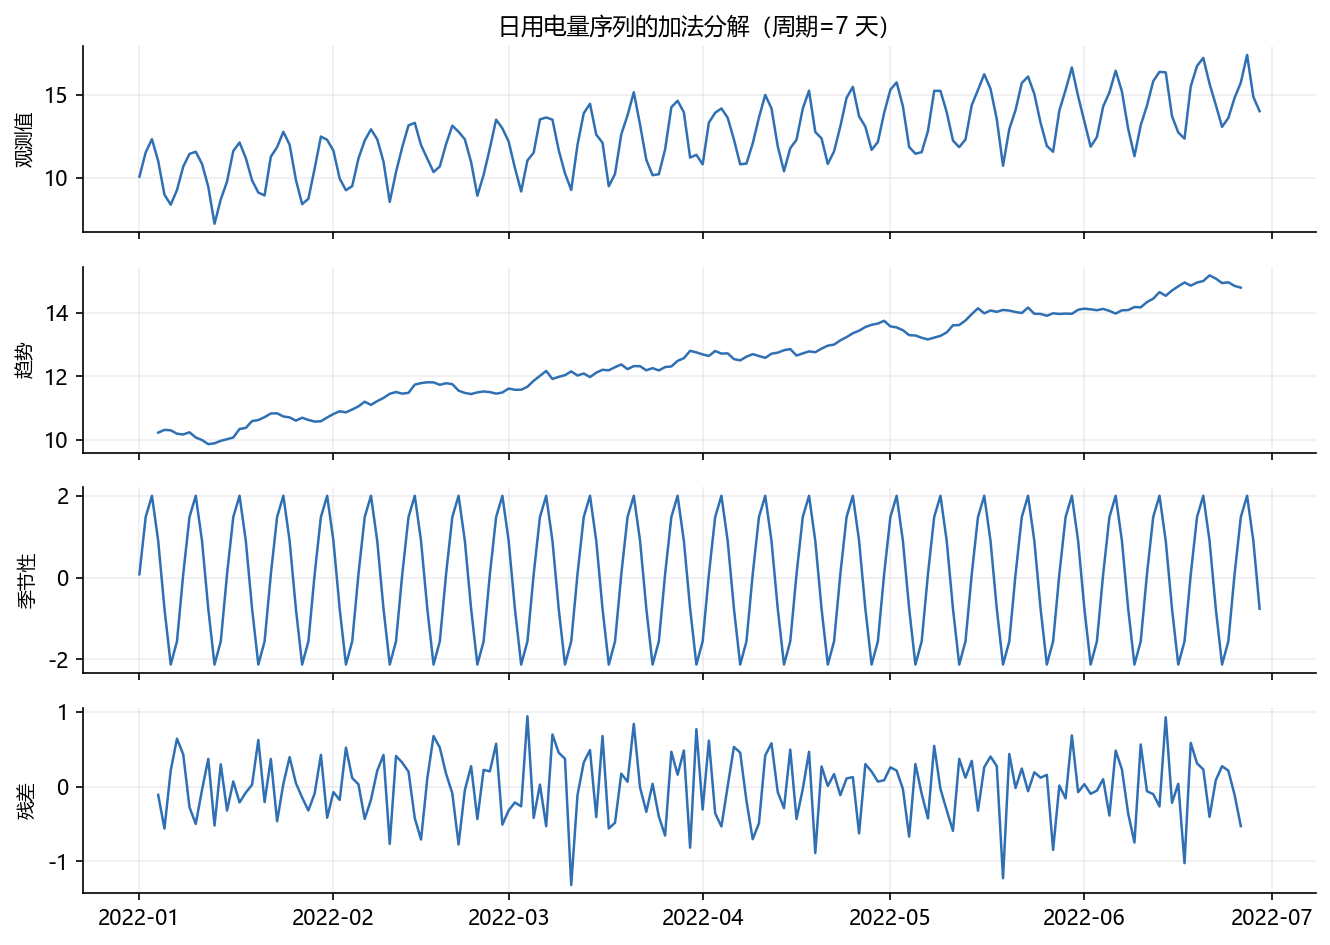
\includegraphics[keepaspectratio,alt={日序列加法分解}]{figures/07-statsmodels/decompose_daily.png}}
\caption{日序列加法分解}
\end{figure}

\textbf{解读}：

\begin{itemize}
\tightlist
\item
  trend 前 3 个是 NaN，因为居中的移动平均在两端没有完整窗口；
\item
  seasonal 在 7 天内正负交替（周一/周末的效应），幅度约 ±2；
\item
  残差均值接近 0、标准差约 0.43，与设定的噪声尺度（0.5）相符。
\end{itemize}

\subsubsection{1.3 月度数据（周期=12
个月）}\label{ux6708ux5ea6ux6570ux636eux5468ux671f12-ux4e2aux6708}

\begin{Shaded}
\begin{Highlighting}[]
\NormalTok{rng }\OperatorTok{=}\NormalTok{ np.random.default\_rng(}\DecValTok{5}\NormalTok{)}
\NormalTok{idxm }\OperatorTok{=}\NormalTok{ pd.date\_range(}\StringTok{\textquotesingle{}2019{-}01{-}01\textquotesingle{}}\NormalTok{, periods}\OperatorTok{=}\DecValTok{36}\NormalTok{, freq}\OperatorTok{=}\StringTok{\textquotesingle{}MS\textquotesingle{}}\NormalTok{)}
\NormalTok{trendm }\OperatorTok{=}\NormalTok{ np.linspace(}\DecValTok{0}\NormalTok{, }\DecValTok{12}\NormalTok{, }\BuiltInTok{len}\NormalTok{(idxm))}
\NormalTok{seasonm }\OperatorTok{=} \DecValTok{3}\OperatorTok{*}\NormalTok{np.sin(}\DecValTok{2}\OperatorTok{*}\NormalTok{np.pi}\OperatorTok{*}\NormalTok{np.arange(}\BuiltInTok{len}\NormalTok{(idxm))}\OperatorTok{/}\DecValTok{12}\NormalTok{)}
\NormalTok{ym }\OperatorTok{=}\NormalTok{ pd.Series(}\DecValTok{50} \OperatorTok{+}\NormalTok{ trendm }\OperatorTok{+}\NormalTok{ seasonm }\OperatorTok{+}\NormalTok{ rng.normal(}\DecValTok{0}\NormalTok{, }\FloatTok{0.8}\NormalTok{, }\BuiltInTok{len}\NormalTok{(idxm)), index}\OperatorTok{=}\NormalTok{idxm)}
\NormalTok{resm }\OperatorTok{=}\NormalTok{ seasonal\_decompose(ym, model}\OperatorTok{=}\StringTok{\textquotesingle{}additive\textquotesingle{}}\NormalTok{, period}\OperatorTok{=}\DecValTok{12}\NormalTok{)}
\BuiltInTok{print}\NormalTok{(}\StringTok{"monthly trend sample:"}\NormalTok{, np.}\BuiltInTok{round}\NormalTok{(resm.trend.dropna().values[:}\DecValTok{4}\NormalTok{], }\DecValTok{3}\NormalTok{))}
\BuiltInTok{print}\NormalTok{(}\StringTok{"monthly seasonal sample:"}\NormalTok{, np.}\BuiltInTok{round}\NormalTok{(resm.seasonal.dropna().values[:}\DecValTok{4}\NormalTok{], }\DecValTok{3}\NormalTok{))}
\end{Highlighting}
\end{Shaded}

运行结果：

\begin{Shaded}
\begin{Highlighting}[]
\NormalTok{monthly trend sample: [52.01  52.446 52.901 53.187]}
\NormalTok{monthly seasonal sample: [{-}0.004  2.686  2.236  2.464]}
\end{Highlighting}
\end{Shaded}

\textbf{注意}：period 必须与实际季节周期一致（日数据 7、月数据
12、季数据
4），数据必须先有\textbf{等间隔、无缺失}的时间索引；若频率已知（如
freq=`D'），可省略 period。

\begin{center}\rule{0.5\linewidth}{0.5pt}\end{center}

\subsection{2 平稳性检验（ADF
单位根检验）}\label{ux5e73ux7a33ux6027ux68c0ux9a8cadf-ux5355ux4f4dux6839ux68c0ux9a8c}

\subsubsection{2.1 概念}\label{ux6982ux5ff5-3}

ARIMA 要求序列\textbf{平稳}（均值、方差不随时间变化）。ADF
检验的原假设是``序列存在单位根（非平稳）''。若 P
值很小（\textless0.05），则拒绝原假设，认为序列平稳。

\subsubsection{2.2 AR(1)
与随机游走对比}\label{ar1-ux4e0eux968fux673aux6e38ux8d70ux5bf9ux6bd4}

\begin{Shaded}
\begin{Highlighting}[]
\ImportTok{import}\NormalTok{ numpy }\ImportTok{as}\NormalTok{ np}
\ImportTok{from}\NormalTok{ statsmodels.tsa.stattools }\ImportTok{import}\NormalTok{ adfuller}

\CommentTok{\#\# 平稳的 AR(1): y\_t = 0.7*y\_\{t{-}1\} + 噪声}
\NormalTok{rng }\OperatorTok{=}\NormalTok{ np.random.default\_rng(}\DecValTok{0}\NormalTok{)}
\NormalTok{n }\OperatorTok{=} \DecValTok{300}
\NormalTok{y\_ar }\OperatorTok{=}\NormalTok{ np.zeros(n)}
\ControlFlowTok{for}\NormalTok{ t }\KeywordTok{in} \BuiltInTok{range}\NormalTok{(}\DecValTok{1}\NormalTok{, n):}
\NormalTok{    y\_ar[t] }\OperatorTok{=} \FloatTok{0.7}\OperatorTok{*}\NormalTok{y\_ar[t}\OperatorTok{{-}}\DecValTok{1}\NormalTok{] }\OperatorTok{+}\NormalTok{ rng.normal(}\DecValTok{0}\NormalTok{, }\DecValTok{1}\NormalTok{)}
\NormalTok{stat1, p1, }\OperatorTok{*}\NormalTok{\_ }\OperatorTok{=}\NormalTok{ adfuller(y\_ar)}
\BuiltInTok{print}\NormalTok{(}\StringTok{"AR(1)        ADF=}\SpecialCharTok{\%.3f}\StringTok{ p=}\SpecialCharTok{\%.3g}\StringTok{"} \OperatorTok{\%}\NormalTok{ (stat1, p1))}

\CommentTok{\#\# 非平稳的随机游走 \textless{}{-}{-}\textgreater{} 单位根}
\NormalTok{rng }\OperatorTok{=}\NormalTok{ np.random.default\_rng(}\DecValTok{1}\NormalTok{)}
\NormalTok{rw }\OperatorTok{=}\NormalTok{ np.cumsum(rng.normal(}\DecValTok{0}\NormalTok{, }\DecValTok{1}\NormalTok{, }\DecValTok{200}\NormalTok{))}
\NormalTok{stat2, p2, }\OperatorTok{*}\NormalTok{\_ }\OperatorTok{=}\NormalTok{ adfuller(rw)}
\BuiltInTok{print}\NormalTok{(}\StringTok{"Random walk  ADF=}\SpecialCharTok{\%.3f}\StringTok{ p=}\SpecialCharTok{\%.3g}\StringTok{"} \OperatorTok{\%}\NormalTok{ (stat2, p2))}
\end{Highlighting}
\end{Shaded}

运行结果：

\begin{Shaded}
\begin{Highlighting}[]
\NormalTok{AR(1)        ADF={-}6.927 p=1.11e{-}09}
\NormalTok{Random walk  ADF={-}0.828 p=0.811}
\end{Highlighting}
\end{Shaded}

\textbf{解读}：

\begin{itemize}
\tightlist
\item
  AR(1) 的 P 值 ≈ 1e-9 \textless{} 0.05，平稳；
\item
  随机游走（单位根）的 P 值 ≈ 0.81 \textgreater{} 0.05，非平稳；
\item
  因此对随机游走类序列，通常先做\textbf{一阶差分} ts.diff().dropna()
  再建模，这就是 ARIMA 中 \(d=1\) 的意义。
\end{itemize}

\begin{center}\rule{0.5\linewidth}{0.5pt}\end{center}

\subsection{3 ARIMA 模型}\label{arima-ux6a21ux578b}

\subsubsection{3.1 概念}\label{ux6982ux5ff5-4}

ARIMA\((p,d,q)\) 由三部分组成：

\begin{itemize}
\tightlist
\item
  \textbf{AR(p)}：用前 \(p\) 个滞后值 \(y_{t-1}, \dots, y_{t-p}\) 回归；
\item
  \textbf{I(d)}：做 \(d\) 次差分使序列平稳；
\item
  \textbf{MA(q)}：用前 \(q\) 个残差项
  \(\varepsilon_{t-1}, \dots, \varepsilon_{t-q}\) 回归。
\end{itemize}

若序列还有季节成分，可扩展为 SARIMA\((p,d,q)(P,D,Q)_s\)。

\subsubsection{3.2 拟合与预测}\label{ux62dfux5408ux4e0eux9884ux6d4b}

用 statsmodels 的 ARIMA 对带趋势的非平稳序列拟合并预测未来 5 步。

\begin{Shaded}
\begin{Highlighting}[]
\ImportTok{import}\NormalTok{ numpy }\ImportTok{as}\NormalTok{ np}
\ImportTok{import}\NormalTok{ pandas }\ImportTok{as}\NormalTok{ pd}
\ImportTok{import}\NormalTok{ matplotlib.pyplot }\ImportTok{as}\NormalTok{ plt}
\ImportTok{from}\NormalTok{ statsmodels.tsa.arima.model }\ImportTok{import}\NormalTok{ ARIMA}

\NormalTok{rng }\OperatorTok{=}\NormalTok{ np.random.default\_rng(}\DecValTok{0}\NormalTok{)}
\NormalTok{n }\OperatorTok{=} \DecValTok{200}
\NormalTok{steps }\OperatorTok{=}\NormalTok{ rng.normal(}\DecValTok{0}\NormalTok{, }\DecValTok{1}\NormalTok{, n).cumsum() }\OperatorTok{+}\NormalTok{ np.linspace(}\DecValTok{0}\NormalTok{, }\DecValTok{10}\NormalTok{, n)}
\NormalTok{si }\OperatorTok{=}\NormalTok{ pd.Series(steps, index}\OperatorTok{=}\NormalTok{pd.date\_range(}\StringTok{\textquotesingle{}2020{-}01{-}01\textquotesingle{}}\NormalTok{, periods}\OperatorTok{=}\NormalTok{n, freq}\OperatorTok{=}\StringTok{\textquotesingle{}D\textquotesingle{}}\NormalTok{))}
\NormalTok{mod }\OperatorTok{=}\NormalTok{ ARIMA(si, order}\OperatorTok{=}\NormalTok{(}\DecValTok{1}\NormalTok{, }\DecValTok{1}\NormalTok{, }\DecValTok{1}\NormalTok{)).fit()}
\BuiltInTok{print}\NormalTok{(mod.summary())}
\NormalTok{fc }\OperatorTok{=}\NormalTok{ mod.forecast(steps}\OperatorTok{=}\DecValTok{5}\NormalTok{)}
\BuiltInTok{print}\NormalTok{(}\StringTok{"forecast:"}\NormalTok{, np.}\BuiltInTok{round}\NormalTok{(fc.values, }\DecValTok{4}\NormalTok{))}
\BuiltInTok{print}\NormalTok{(}\StringTok{"arparams:"}\NormalTok{, mod.arparams, }\StringTok{"maparams:"}\NormalTok{, mod.maparams)}
\end{Highlighting}
\end{Shaded}

运行结果（Date/Time 随运行时间变化）：

\begin{Shaded}
\begin{Highlighting}[]
\NormalTok{                               SARIMAX Results}
\NormalTok{==============================================================================}
\NormalTok{Dep. Variable:                      y   No. Observations:                  200}
\NormalTok{Model:                 ARIMA(1, 1, 1)   Log Likelihood                {-}274.795}
\NormalTok{Date:                Wed, 26 Aug 2026   AIC                            555.589}
\NormalTok{Time:                        14:08:43   BIC                            565.469}
\NormalTok{Sample:                    01{-}01{-}2020   HQIC                           559.588}
\NormalTok{                         {-} 07{-}18{-}2020}
\NormalTok{Covariance Type:                  opg}
\NormalTok{==============================================================================}
\NormalTok{                 coef    std err          z      P\textgreater{}|z|      [0.025      0.975]}
\NormalTok{{-}{-}{-}{-}{-}{-}{-}{-}{-}{-}{-}{-}{-}{-}{-}{-}{-}{-}{-}{-}{-}{-}{-}{-}{-}{-}{-}{-}{-}{-}{-}{-}{-}{-}{-}{-}{-}{-}{-}{-}{-}{-}{-}{-}{-}{-}{-}{-}{-}{-}{-}{-}{-}{-}{-}{-}{-}{-}{-}{-}{-}{-}{-}{-}{-}{-}{-}{-}{-}{-}{-}{-}{-}{-}{-}{-}{-}{-}}
\NormalTok{ar.L1          0.6440      0.614      1.049      0.294      {-}0.559       1.847}
\NormalTok{ma.L1         {-}0.5829      0.658     {-}0.886      0.376      {-}1.872       0.707}
\NormalTok{sigma2         0.9266      0.105      8.800      0.000       0.720       1.133}
\NormalTok{===================================================================================}
\NormalTok{Ljung{-}Box (L1) (Q):                   0.15   Jarque{-}Bera (JB):                 2.63}
\NormalTok{Prob(Q):                              0.70   Prob(JB):                         0.27}
\NormalTok{Heteroskedasticity (H):               1.17   Skew:                            {-}0.21}
\NormalTok{Prob(H) (two{-}sided):                  0.52   Kurtosis:                         2.63}
\NormalTok{===================================================================================}

\NormalTok{Warnings:}
\NormalTok{[1] Covariance matrix calculated using the outer product of gradients (complex{-}step).}

\NormalTok{forecast: [13.0612 13.0667 13.0702 13.0725 13.074 ]}
\NormalTok{arparams: [0.64404169] maparams: [{-}0.58293935]}
\end{Highlighting}
\end{Shaded}

\begin{figure}
\centering
\pandocbounded{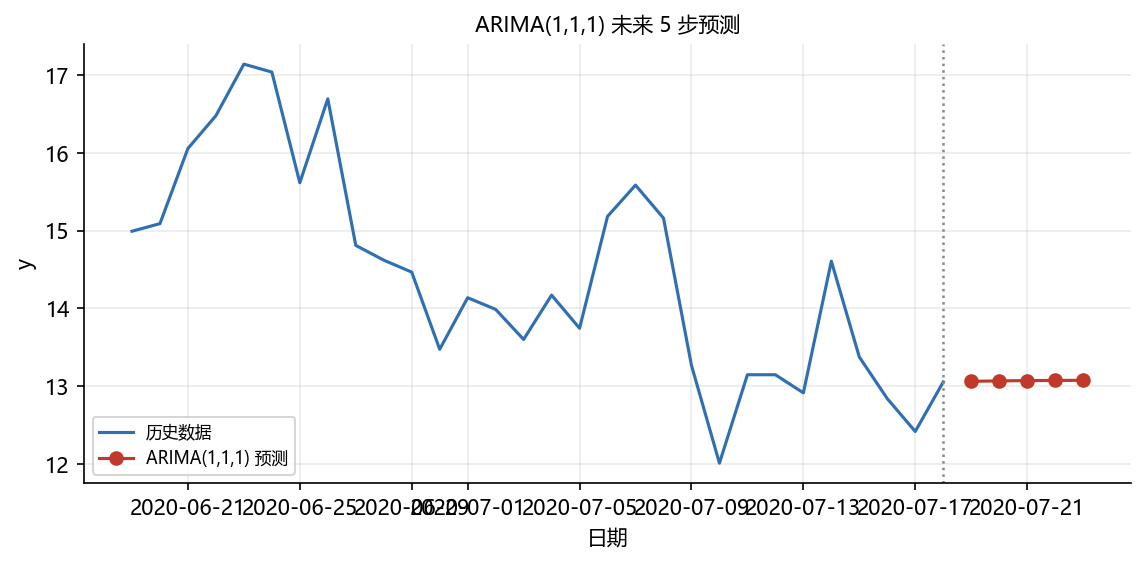
\includegraphics[keepaspectratio,alt={ARIMA 未来 5 步预测}]{figures/07-statsmodels/arima_forecast.png}}
\caption{ARIMA 未来 5 步预测}
\end{figure}

\textbf{解读}：

\begin{itemize}
\tightlist
\item
  ar.L1 与 ma.L1 是 AR(1) 与 MA(1) 系数；本例两者 P
  值都较大（不显著），提示该阶 \((1,1,1)\)
  可能略偏大，但这不影响演示流程；
\item
  forecast 给出未来 5 个时间点的预测值（约 13.06 → 13.07）；
\item
  Prob(JB)=0.27 说明残差近似正态；Prob(Ljung-Box)
  用来检查残差是否还有自相关。
\end{itemize}

\subsubsection{3.3 如何选择 (p, d,
q)}\label{ux5982ux4f55ux9009ux62e9-p-d-q}

\begin{itemize}
\tightlist
\item
  \textbf{d}：由 ADF 检验决定，不平稳就差分；
\item
  \textbf{p / q}：看 ACF 与 PACF 图。ACF 截尾选 MA，PACF 截尾选
  AR；也可用 statsmodels.tsa.stattools.acf/pacf 或网格搜索（如
  itertools.product + AIC）。
\end{itemize}

\begin{Shaded}
\begin{Highlighting}[]
\ImportTok{from}\NormalTok{ statsmodels.tsa.stattools }\ImportTok{import}\NormalTok{ acf, pacf}
\NormalTok{ac }\OperatorTok{=}\NormalTok{ acf(si, nlags}\OperatorTok{=}\DecValTok{5}\NormalTok{)}
\NormalTok{pc }\OperatorTok{=}\NormalTok{ pacf(si, nlags}\OperatorTok{=}\DecValTok{5}\NormalTok{)}
\BuiltInTok{print}\NormalTok{(}\StringTok{"ACF:"}\NormalTok{, np.}\BuiltInTok{round}\NormalTok{(ac, }\DecValTok{3}\NormalTok{))}
\BuiltInTok{print}\NormalTok{(}\StringTok{"PACF:"}\NormalTok{, np.}\BuiltInTok{round}\NormalTok{(pc, }\DecValTok{3}\NormalTok{))}
\end{Highlighting}
\end{Shaded}

运行结果：

\begin{Shaded}
\begin{Highlighting}[]
\NormalTok{ACF:  [1.    0.983 0.965 0.946 0.927 0.906]}
\NormalTok{PACF: [ 1.     0.988 {-}0.045 {-}0.068 {-}0.003 {-}0.108]}
\end{Highlighting}
\end{Shaded}

本例序列 ACF 缓慢衰减（非平稳特征），PACF
在一阶后急剧下降，提示需要先差分。

\begin{quote}
运行时会看到 ``Non-stationary starting autoregressive parameters found /
Non-invertible starting MA parameters'' 之类的提示，属正常，statsmodels
会改用零值作为初始参数。
\end{quote}

\subsection{案例卡 3：ARIMA 时间序列------用 ADF 检验与残差诊断选
p,d,q}\label{ux6848ux4f8bux5361-3arima-ux65f6ux95f4ux5e8fux5217ux7528-adf-ux68c0ux9a8cux4e0eux6b8bux5deeux8bcaux65adux9009-pdq}

\subsubsection{目标}\label{ux76eeux6807-29}

模拟一个``先平稳、再被累加''的 ARIMA(1,1,1)
序列，完整走一遍选阶流程：先用 \textbf{ADF} 定差分阶数
\texttt{d}，再看差分序列的 \textbf{ACF/PACF} 与网格搜索（AIC）定
\texttt{p}、\texttt{q}，最后用 \textbf{Ljung-Box} 与
\textbf{Jarque-Bera} 检查残差是否``洗干净''成白噪声，并给出未来 5
步预测。

\subsubsection{代码}\label{ux4ee3ux7801-30}

\begin{Shaded}
\begin{Highlighting}[]
\ImportTok{import}\NormalTok{ numpy }\ImportTok{as}\NormalTok{ np}
\ImportTok{import}\NormalTok{ pandas }\ImportTok{as}\NormalTok{ pd}
\ImportTok{import}\NormalTok{ warnings}
\NormalTok{warnings.filterwarnings(}\StringTok{\textquotesingle{}ignore\textquotesingle{}}\NormalTok{)}
\ImportTok{from}\NormalTok{ statsmodels.tsa.stattools }\ImportTok{import}\NormalTok{ adfuller, acf, pacf}
\ImportTok{from}\NormalTok{ statsmodels.tsa.arima.model }\ImportTok{import}\NormalTok{ ARIMA}
\ImportTok{from}\NormalTok{ statsmodels.stats.diagnostic }\ImportTok{import}\NormalTok{ acorr\_ljungbox}
\ImportTok{from}\NormalTok{ statsmodels.stats.stattools }\ImportTok{import}\NormalTok{ jarque\_bera}
\ImportTok{from}\NormalTok{ statsmodels.graphics.tsaplots }\ImportTok{import}\NormalTok{ plot\_acf}
\ImportTok{from}\NormalTok{ itertools }\ImportTok{import}\NormalTok{ product}
\ImportTok{import}\NormalTok{ matplotlib.pyplot }\ImportTok{as}\NormalTok{ plt}
\ImportTok{import}\NormalTok{ os}

\NormalTok{plt.rcParams[}\StringTok{\textquotesingle{}font.sans{-}serif\textquotesingle{}}\NormalTok{] }\OperatorTok{=}\NormalTok{ [}\StringTok{\textquotesingle{}Microsoft YaHei\textquotesingle{}}\NormalTok{, }\StringTok{\textquotesingle{}SimHei\textquotesingle{}}\NormalTok{, }\StringTok{\textquotesingle{}DejaVu Sans\textquotesingle{}}\NormalTok{]}
\NormalTok{plt.rcParams[}\StringTok{\textquotesingle{}axes.unicode\_minus\textquotesingle{}}\NormalTok{] }\OperatorTok{=} \VariableTok{False}
\NormalTok{np.set\_printoptions(precision}\OperatorTok{=}\DecValTok{4}\NormalTok{, suppress}\OperatorTok{=}\VariableTok{True}\NormalTok{)}
\NormalTok{pd.set\_option(}\StringTok{\textquotesingle{}display.width\textquotesingle{}}\NormalTok{, }\DecValTok{100}\NormalTok{)}

\NormalTok{rng }\OperatorTok{=}\NormalTok{ np.random.default\_rng(}\DecValTok{11}\NormalTok{)}
\NormalTok{n }\OperatorTok{=} \DecValTok{300}
\NormalTok{e }\OperatorTok{=}\NormalTok{ rng.normal(}\DecValTok{0}\NormalTok{, }\DecValTok{1}\NormalTok{, n)}
\NormalTok{x }\OperatorTok{=}\NormalTok{ np.zeros(n)}
\ControlFlowTok{for}\NormalTok{ t }\KeywordTok{in} \BuiltInTok{range}\NormalTok{(}\DecValTok{1}\NormalTok{, n):}
\NormalTok{    x[t] }\OperatorTok{=} \FloatTok{0.6}\OperatorTok{*}\NormalTok{x[t}\OperatorTok{{-}}\DecValTok{1}\NormalTok{] }\OperatorTok{+}\NormalTok{ e[t] }\OperatorTok{+} \FloatTok{0.3}\OperatorTok{*}\NormalTok{e[t}\OperatorTok{{-}}\DecValTok{1}\NormalTok{]      }\CommentTok{\# 平稳的 ARMA(1,1)}
\NormalTok{vals }\OperatorTok{=}\NormalTok{ np.cumsum(x) }\OperatorTok{+} \DecValTok{100}                      \CommentTok{\# 累加 =\textgreater{} ARIMA(1,1,1)}
\NormalTok{idx }\OperatorTok{=}\NormalTok{ pd.date\_range(}\StringTok{\textquotesingle{}2020{-}01{-}01\textquotesingle{}}\NormalTok{, periods}\OperatorTok{=}\NormalTok{n, freq}\OperatorTok{=}\StringTok{\textquotesingle{}D\textquotesingle{}}\NormalTok{)}
\NormalTok{ser }\OperatorTok{=}\NormalTok{ pd.Series(vals, index}\OperatorTok{=}\NormalTok{idx)}

\NormalTok{adf0 }\OperatorTok{=}\NormalTok{ adfuller(ser)}
\BuiltInTok{print}\NormalTok{(}\StringTok{\textquotesingle{}adfuller raw: ADF=}\SpecialCharTok{\%.3f}\StringTok{ p=}\SpecialCharTok{\%.3g}\StringTok{\textquotesingle{}} \OperatorTok{\%}\NormalTok{ (adf0[}\DecValTok{0}\NormalTok{], adf0[}\DecValTok{1}\NormalTok{]))}
\NormalTok{d1 }\OperatorTok{=}\NormalTok{ ser.diff().dropna()}
\NormalTok{adf1 }\OperatorTok{=}\NormalTok{ adfuller(d1)}
\BuiltInTok{print}\NormalTok{(}\StringTok{\textquotesingle{}adfuller diff: ADF=}\SpecialCharTok{\%.3f}\StringTok{ p=}\SpecialCharTok{\%.3g}\StringTok{\textquotesingle{}} \OperatorTok{\%}\NormalTok{ (adf1[}\DecValTok{0}\NormalTok{], adf1[}\DecValTok{1}\NormalTok{]))}
\BuiltInTok{print}\NormalTok{(}\StringTok{\textquotesingle{}ACF(diff) lag1{-}4:\textquotesingle{}}\NormalTok{, np.}\BuiltInTok{round}\NormalTok{(acf(d1, nlags}\OperatorTok{=}\DecValTok{4}\NormalTok{)[}\DecValTok{1}\NormalTok{:], }\DecValTok{3}\NormalTok{))}
\BuiltInTok{print}\NormalTok{(}\StringTok{\textquotesingle{}PACF(diff) lag1{-}4:\textquotesingle{}}\NormalTok{, np.}\BuiltInTok{round}\NormalTok{(pacf(d1, nlags}\OperatorTok{=}\DecValTok{4}\NormalTok{)[}\DecValTok{1}\NormalTok{:], }\DecValTok{3}\NormalTok{))}

\NormalTok{best }\OperatorTok{=} \VariableTok{None}
\ControlFlowTok{for}\NormalTok{ p }\KeywordTok{in} \BuiltInTok{range}\NormalTok{(}\DecValTok{3}\NormalTok{):}
    \ControlFlowTok{for}\NormalTok{ q }\KeywordTok{in} \BuiltInTok{range}\NormalTok{(}\DecValTok{3}\NormalTok{):}
        \ControlFlowTok{try}\NormalTok{:}
\NormalTok{            mod }\OperatorTok{=}\NormalTok{ ARIMA(ser, order}\OperatorTok{=}\NormalTok{(p, }\DecValTok{1}\NormalTok{, q)).fit()}
\NormalTok{            aic }\OperatorTok{=}\NormalTok{ mod.aic}
            \ControlFlowTok{if}\NormalTok{ best }\KeywordTok{is} \VariableTok{None} \KeywordTok{or}\NormalTok{ aic }\OperatorTok{\textless{}}\NormalTok{ best[}\DecValTok{0}\NormalTok{]:}
\NormalTok{                best }\OperatorTok{=}\NormalTok{ (aic, p, q)}
        \ControlFlowTok{except} \PreprocessorTok{Exception}\NormalTok{:}
            \ControlFlowTok{pass}
\BuiltInTok{print}\NormalTok{(}\StringTok{\textquotesingle{}best AIC order (p,d,q):\textquotesingle{}}\NormalTok{, best[}\DecValTok{1}\NormalTok{], }\DecValTok{1}\NormalTok{, best[}\DecValTok{2}\NormalTok{], }\StringTok{\textquotesingle{} AIC=}\SpecialCharTok{\%.3f}\StringTok{\textquotesingle{}} \OperatorTok{\%}\NormalTok{ best[}\DecValTok{0}\NormalTok{])}

\NormalTok{final }\OperatorTok{=}\NormalTok{ ARIMA(ser, order}\OperatorTok{=}\NormalTok{(best[}\DecValTok{1}\NormalTok{], }\DecValTok{1}\NormalTok{, best[}\DecValTok{2}\NormalTok{])).fit()}
\BuiltInTok{print}\NormalTok{(}\StringTok{\textquotesingle{}AR params:\textquotesingle{}}\NormalTok{, np.}\BuiltInTok{round}\NormalTok{(final.arparams, }\DecValTok{4}\NormalTok{))}
\BuiltInTok{print}\NormalTok{(}\StringTok{\textquotesingle{}MA params:\textquotesingle{}}\NormalTok{, np.}\BuiltInTok{round}\NormalTok{(final.maparams, }\DecValTok{4}\NormalTok{))}
\NormalTok{resid }\OperatorTok{=}\NormalTok{ final.resid.iloc[}\DecValTok{10}\NormalTok{:]}
\NormalTok{lb }\OperatorTok{=}\NormalTok{ acorr\_ljungbox(resid, lags}\OperatorTok{=}\NormalTok{[}\DecValTok{10}\NormalTok{], return\_df}\OperatorTok{=}\VariableTok{True}\NormalTok{)}
\NormalTok{jb }\OperatorTok{=}\NormalTok{ jarque\_bera(resid)}
\BuiltInTok{print}\NormalTok{(}\StringTok{\textquotesingle{}Ljung{-}Box Q pvalue = }\SpecialCharTok{\%.4f}\StringTok{\textquotesingle{}} \OperatorTok{\%}\NormalTok{ lb[}\StringTok{\textquotesingle{}lb\_pvalue\textquotesingle{}}\NormalTok{].iloc[}\DecValTok{0}\NormalTok{])}
\BuiltInTok{print}\NormalTok{(}\StringTok{\textquotesingle{}Jarque{-}Bera pvalue = }\SpecialCharTok{\%.4f}\StringTok{\textquotesingle{}} \OperatorTok{\%}\NormalTok{ jb[}\DecValTok{1}\NormalTok{])}
\BuiltInTok{print}\NormalTok{(}\StringTok{\textquotesingle{}forecast 5:\textquotesingle{}}\NormalTok{, np.}\BuiltInTok{round}\NormalTok{(final.forecast(}\DecValTok{5}\NormalTok{).values, }\DecValTok{3}\NormalTok{))}

\NormalTok{os.makedirs(}\StringTok{\textquotesingle{}images\textquotesingle{}}\NormalTok{, exist\_ok}\OperatorTok{=}\VariableTok{True}\NormalTok{)}
\NormalTok{fig, axes }\OperatorTok{=}\NormalTok{ plt.subplots(}\DecValTok{2}\NormalTok{, }\DecValTok{2}\NormalTok{, figsize}\OperatorTok{=}\NormalTok{(}\FloatTok{9.5}\NormalTok{, }\FloatTok{5.6}\NormalTok{))}
\NormalTok{axes[}\DecValTok{0}\NormalTok{,}\DecValTok{0}\NormalTok{].plot(ser.index, ser.values, lw}\OperatorTok{=}\FloatTok{1.1}\NormalTok{, color}\OperatorTok{=}\StringTok{\textquotesingle{}\#2f6fb3\textquotesingle{}}\NormalTok{)}
\NormalTok{axes[}\DecValTok{0}\NormalTok{,}\DecValTok{0}\NormalTok{].set\_title(}\StringTok{\textquotesingle{}原始序列（非平稳）\textquotesingle{}}\NormalTok{)}
\NormalTok{axes[}\DecValTok{0}\NormalTok{,}\DecValTok{1}\NormalTok{].plot(d1.index, d1.values, lw}\OperatorTok{=}\FloatTok{1.1}\NormalTok{, color}\OperatorTok{=}\StringTok{\textquotesingle{}\#3a8f4f\textquotesingle{}}\NormalTok{)}
\NormalTok{axes[}\DecValTok{0}\NormalTok{,}\DecValTok{1}\NormalTok{].set\_title(}\StringTok{\textquotesingle{}一阶差分\textquotesingle{}}\NormalTok{)}
\NormalTok{plot\_acf(d1, ax}\OperatorTok{=}\NormalTok{axes[}\DecValTok{1}\NormalTok{,}\DecValTok{0}\NormalTok{], lags}\OperatorTok{=}\DecValTok{15}\NormalTok{, title}\OperatorTok{=}\StringTok{\textquotesingle{}差分 ACF\textquotesingle{}}\NormalTok{)}
\NormalTok{plot\_acf(resid, ax}\OperatorTok{=}\NormalTok{axes[}\DecValTok{1}\NormalTok{,}\DecValTok{1}\NormalTok{], lags}\OperatorTok{=}\DecValTok{15}\NormalTok{, title}\OperatorTok{=}\StringTok{\textquotesingle{}残差 ACF\textquotesingle{}}\NormalTok{)}
\ControlFlowTok{for}\NormalTok{ ax }\KeywordTok{in}\NormalTok{ axes.ravel():}
\NormalTok{    ax.grid(alpha}\OperatorTok{=}\FloatTok{0.2}\NormalTok{)}
\NormalTok{fig.tight\_layout()}
\NormalTok{fig.savefig(}\StringTok{\textquotesingle{}figures/07{-}statsmodels/case3\_arima\_diag.png\textquotesingle{}}\NormalTok{, dpi}\OperatorTok{=}\DecValTok{150}\NormalTok{)}
\NormalTok{plt.close()}
\BuiltInTok{print}\NormalTok{(}\StringTok{\textquotesingle{}saved figures/07{-}statsmodels/case3\_arima\_diag.png\textquotesingle{}}\NormalTok{)}
\end{Highlighting}
\end{Shaded}

\subsubsection{运行结果（已运行核验）}\label{ux8fd0ux884cux7ed3ux679cux5df2ux8fd0ux884cux6838ux9a8c-28}

\begin{Shaded}
\begin{Highlighting}[]
\NormalTok{adfuller raw: ADF={-}2.239 p=0.192}
\NormalTok{adfuller diff: ADF={-}6.094 p=1.02e{-}07}
\NormalTok{ACF(diff) lag1{-}4: [0.738 0.457 0.311 0.202]}
\NormalTok{PACF(diff) lag1{-}4: [ 0.741 {-}0.196  0.119 {-}0.071]}
\NormalTok{best AIC order (p,d,q): 1 1 1  AIC=802.817}
\NormalTok{AR params: [0.5958]}
\NormalTok{MA params: [0.3302]}
\NormalTok{Ljung{-}Box Q pvalue = 0.2587}
\NormalTok{Jarque{-}Bera pvalue = 0.4776}
\NormalTok{forecast 5: [122.494 121.879 121.512 121.294 121.164]}
\NormalTok{saved figures/07{-}statsmodels/case3\_arima\_diag.png}
\end{Highlighting}
\end{Shaded}

\subsubsection{讲解}\label{ux8bb2ux89e3-28}

\textbf{一句话解释}：先问``序列稳不稳''（ADF），不稳就先差分（\texttt{d}=1）；再用``多少阶自相关/移动平均''（ACF/PACF
+ AIC）挑
\texttt{p}、\texttt{q}；最后看残差是不是``没剩什么信息''（Ljung-Box /
JB）来确认模型合格。

\begin{enumerate}
\def\labelenumi{\arabic{enumi}.}
\tightlist
\item
  \texttt{x{[}t{]}=0.6*x{[}t-1{]}+e{[}t{]}+0.3*e{[}t-1{]}}
  造一个\textbf{平稳} ARMA(1,1)；再 \texttt{np.cumsum(x)} 累加得到
  \texttt{ARIMA(1,1,1)} 序列（差分后就是原来的
  ARMA）。这样做能让我们``知道答案''，方便验证流程。
\item
  \texttt{adfuller(ser)}：原始序列
  \texttt{p=0.192\ \textgreater{}\ 0.05}，不能拒绝单位根，说明\textbf{非平稳}
  → 决定 \texttt{d=1}。
\item
  \texttt{ser.diff().dropna()}：一阶差分后再做
  ADF，\texttt{p=1.02e-07\ \textless{}\ 0.05}，差分序列\textbf{平稳}。
\item
  ACF/PACF 只是``参考图''：差分序列 ACF 在 lag1 就衰减到 0.74，PACF 也是
  lag1 最大，说明滞后阶数不需要太大。
\item
  网格搜索（\texttt{itertools.product}）在
  \texttt{p,q\ in\ \{0,1,2\}}、固定 \texttt{d=1} 下比较 AIC，选出
  \texttt{(1,1,1)}（AIC=802.817），与真实阶数一致。
\item
  结果解读：\texttt{AR(1)=0.596}、\texttt{MA(1)=0.330} 都接近生成时的
  0.6 与 0.3；\texttt{Ljung-Box\ p=0.259}、\texttt{Jarque-Bera\ p=0.478}
  都大于 0.05，说明残差\textbf{近似白噪声}，模型合格。
\item
  \texttt{forecast(5)} 给出未来 5 天（约 122.5 →
  121.2）的预测；画图里``残差
  ACF''几乎都在置信带内，也支持``残差已洗净''。
\end{enumerate}

\begin{figure}
\centering
\pandocbounded{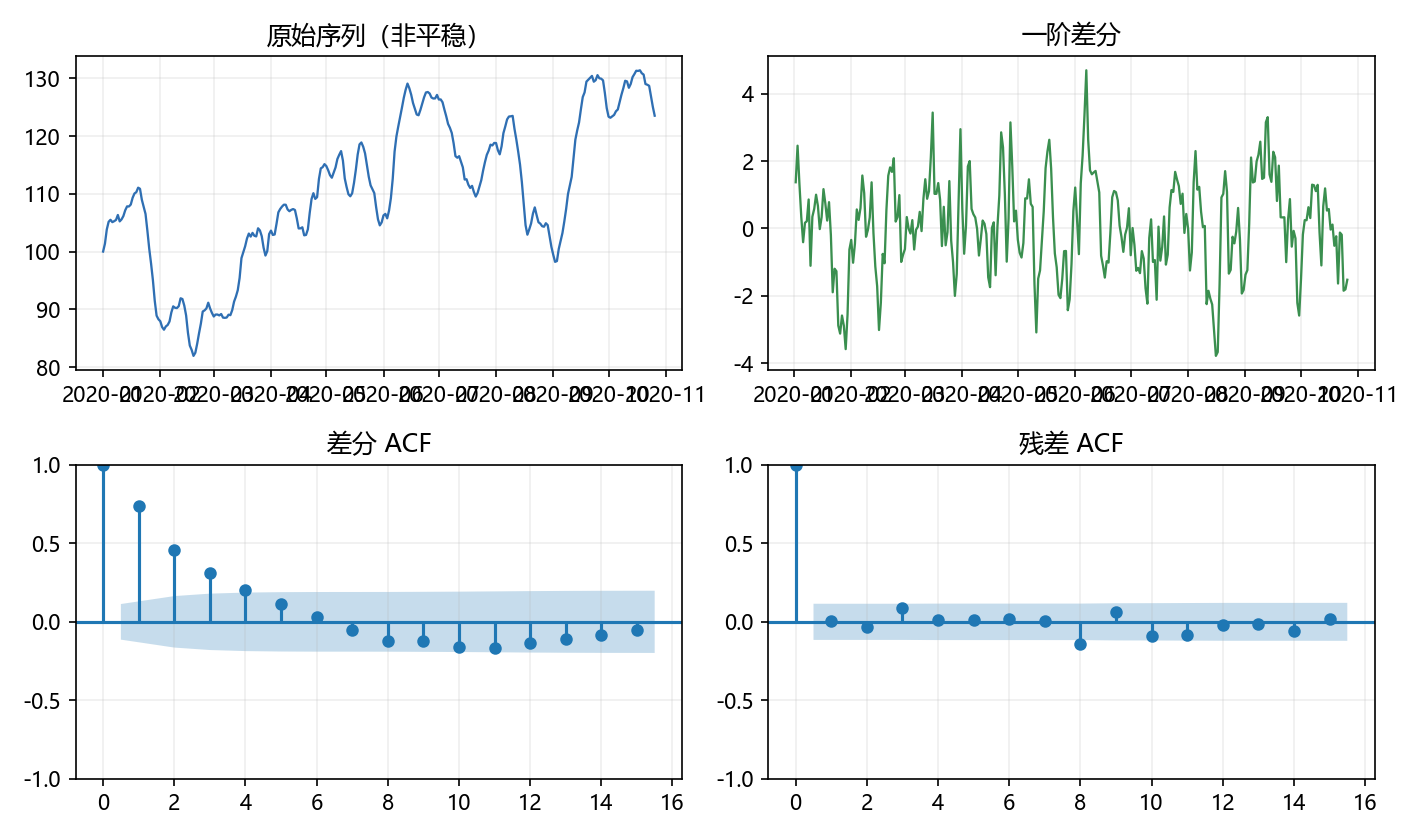
\includegraphics[keepaspectratio,alt={ARIMA 选阶与残差诊断图}]{figures/07-statsmodels/case3_arima_diag.png}}
\caption{ARIMA 选阶与残差诊断图}
\end{figure}

\subsubsection{主要用法 / API}\label{ux4e3bux8981ux7528ux6cd5-api-30}

{\def\LTcaptype{none} % do not increment counter
\begin{longtable}[]{@{}
  >{\raggedright\arraybackslash}p{(\linewidth - 4\tabcolsep) * \real{0.3333}}
  >{\raggedright\arraybackslash}p{(\linewidth - 4\tabcolsep) * \real{0.3333}}
  >{\raggedright\arraybackslash}p{(\linewidth - 4\tabcolsep) * \real{0.3333}}@{}}
\toprule\noalign{}
\begin{minipage}[b]{\linewidth}\raggedright
需求
\end{minipage} & \begin{minipage}[b]{\linewidth}\raggedright
写法
\end{minipage} & \begin{minipage}[b]{\linewidth}\raggedright
说明
\end{minipage} \\
\midrule\noalign{}
\endhead
\bottomrule\noalign{}
\endlastfoot
平稳性检验 & \texttt{adfuller(ser)} & 返回 (ADF, p, \ldots) \\
差分 & \texttt{ser.diff().dropna()} & \texttt{diff()} 后首元素为 NaN \\
ACF/PACF & \texttt{acf(d1,\ nlags=4)} / \texttt{pacf(...)} & 判断 p/q
参考 \\
网格选阶 & \texttt{itertools.product(range(3),\ range(3))} + AIC &
在候选 (p,q) 中找 AIC 最小 \\
拟合 ARIMA & \texttt{ARIMA(ser,\ order=(p,d,q)).fit()} &
返回模型（含预测） \\
残差自相关 & \texttt{acorr\_ljungbox(resid,\ lags={[}10{]})} &
p\textgreater0.05 视为白噪声 \\
残差正态性 & \texttt{jarque\_bera(resid)} & p\textgreater0.05
可接受正态 \\
预测 & \texttt{model.forecast(steps=5)} & 返回未来值 \\
\end{longtable}
}

\subsubsection{常见错误}\label{ux5e38ux89c1ux9519ux8bef-30}

\begin{enumerate}
\def\labelenumi{\arabic{enumi}.}
\tightlist
\item
  拿到序列就拟合 ARIMA，不做
  ADF：非平稳序列容易``伪回归''，应先检验、必要时差分。
\item
  \texttt{diff()} 后忘记 \texttt{dropna()}：首元素为
  NaN，\texttt{adfuller} 或 \texttt{acf} 会报错。
\item
  直接用 \texttt{final.resid} 做诊断：模型首期残差可能因初始化偏大，建议
  \texttt{resid.iloc{[}10:{]}} 跳过 burn-in 再检验。
\item
  只看 \texttt{summary()} 的 AIC/BIC 而不做残差诊断：AIC
  低不代表残差是白噪声，仍需 Ljung-Box 与 JB。
\item
  网格搜索时把所有阶数都 \texttt{fit()}，可能触发``Non-stationary
  starting\ldots''等提示；用
  \texttt{warnings.filterwarnings(\textquotesingle{}ignore\textquotesingle{})}
  只影响显示，不影响结果。
\end{enumerate}

\subsubsection{拓展 / 跟练}\label{ux62d3ux5c55-ux8ddfux7ec3-18}

\begin{enumerate}
\def\labelenumi{\arabic{enumi}.}
\tightlist
\item
  把生成模型改成 \texttt{ARIMA(2,1,1)}（在 \texttt{x{[}t{]}} 里加
  \texttt{x{[}t-2{]}} 项），看网格搜索是否选回 \texttt{(2,1,1)}。
\item
  把 \texttt{lags} 换成 \texttt{{[}5,\ 20{]}}，分别看 Ljung-Box p
  值，理解滞后阶数的影响。
\item
  用 \texttt{statsmodels.tsa.statespace.SARIMAX} 加入季节项
  \texttt{(1,1,1)(1,1,1,7)}，比较与普通 ARIMA 的 AIC。
\item
  把数据切为训练/测试（前 240 / 后 60），用 RMSE 比较
  \texttt{ARIMA(1,1,1)}、\texttt{ARIMA(2,1,1)} 与 \texttt{ARIMA(0,1,0)}
  谁的预测误差最小。
\end{enumerate}

\begin{center}\rule{0.5\linewidth}{0.5pt}\end{center}

\subsection{常见误区}\label{ux5e38ux89c1ux8befux533a-21}

\begin{enumerate}
\def\labelenumi{\arabic{enumi}.}
\tightlist
\item
  \textbf{忘了先检查平稳性}：直接对非平稳序列拟合 ARIMA
  可能得到``伪回归''。
\item
  \textbf{分解前不处理缺失/等间隔}：seasonal\_decompose
  要求完整、等间隔的时间索引。
\item
  \textbf{period 设错}：日数据应为 7，月数据应为 12；设成 1
  会失去季节意义。
\item
  \textbf{预测时不会生成未来索引}：forecast(steps=5)
  返回数值，需自己构造 pd.date\_range 画图。
\item
  \textbf{只看 AIC 不看病灶}：AIC 低不保证残差是白噪声；应同时看
  Ljung-Box 与 JB。
\item
  \textbf{diff() 后不 dropna()}：差分会产生一个 NaN，需 dropna()
  或忽略。
\end{enumerate}

\subsection{思考题}\label{ux601dux8003ux9898-23}

\begin{enumerate}
\def\labelenumi{\arabic{enumi}.}
\tightlist
\item
  加法模型与乘法模型分别适用于什么场景？如何用 result.seasonal
  判断该用哪个？
\item
  为什么随机游走序列 ADF 检验的 P 值很大？一阶差分后其 ADF P 值会怎样？
\item
  ARIMA\((2,1,0)\) 与 ARIMA\((0,1,2)\) 分别对应什么模型？画出它们的
  ACF/PACF 有何不同？
\item
  用 forecast(steps=5) 得到未来 5
  步，若数据是月度序列，应如何构造未来时间轴？
\end{enumerate}

\subsection{动手练习（详见
lab）}\label{ux52a8ux624bux7ec3ux4e60ux8be6ux89c1-lab-15}

\begin{itemize}
\tightlist
\item
  构造 180 天日序列，分解并画图，说明周期；
\item
  对 AR(1) 与随机游走做 ADF 检验，比较 P 值；
\item
  用 ARIMA(1,1,1) 拟合，给出未来 5 步预测并画图；
\item
  对带周季节性的日负荷序列，尝试 SARIMAX 或先差分再 ARIMA。
\end{itemize}

\subsection{延伸阅读}\label{ux5ef6ux4f38ux9605ux8bfb-32}

\begin{itemize}
\tightlist
\item
  statsmodels
  时间序列官方：\href{https://www.statsmodels.org/stable/tsa.html}{链接}
\item
  Seasonal-Trend
  decomposition（STL）：\href{https://www.statsmodels.org/devel/examples/notebooks/generated/stl_decomposition.html}{链接}
\item
  Statsmodels
  时间序列官方示例集：\href{https://www.statsmodels.org/stable/examples/index.html\#time-series}{链接}
\end{itemize}

\section{03
综合案例：城市日负荷的统计建模与预测}\label{ux7efcux5408ux6848ux4f8bux57ceux5e02ux65e5ux8d1fux8377ux7684ux7edfux8ba1ux5efaux6a21ux4e0eux9884ux6d4b}

\begin{quote}
本章综合案例，把 \textbf{方差分析 + 线性回归 + 时间序列}
串在一份模拟数据上，体会 Statsmodels 的完整工作流。
配图：figures/07-statsmodels/case\_regression\_diag.png、figures/07-statsmodels/case\_ts\_forecast.png（由
build/make\_chap7\_figures.py 生成）。
\end{quote}

\subsection{背景}\label{ux80ccux666f-6}

某市电网记录了 2023-01-01 起连续 140
天的\textbf{日负荷}（负荷越高用电越多）。我们关心三件事：

\begin{enumerate}
\def\labelenumi{\arabic{enumi}.}
\tightlist
\item
  工作日与周末的日均负荷是否显著不同（\textbf{单因素方差分析}）；
\item
  负荷多大程度上可由\textbf{当日气温}与\textbf{是否周末}解释（\textbf{多元线性回归}）；
\item
  未来的日负荷如何变化（\textbf{时间序列分解 + ARIMA 预测}）。
\end{enumerate}

为便于教学，数据是\textbf{带趋势、周季节、温度效应、周末效应与噪声}的模拟序列。

\subsection{数据构造}\label{ux6570ux636eux6784ux9020}

\begin{Shaded}
\begin{Highlighting}[]
\ImportTok{import}\NormalTok{ numpy }\ImportTok{as}\NormalTok{ np}
\ImportTok{import}\NormalTok{ pandas }\ImportTok{as}\NormalTok{ pd}
\ImportTok{import}\NormalTok{ statsmodels.api }\ImportTok{as}\NormalTok{ sm}
\ImportTok{from}\NormalTok{ statsmodels.formula.api }\ImportTok{import}\NormalTok{ ols}
\ImportTok{from}\NormalTok{ statsmodels.tsa.seasonal }\ImportTok{import}\NormalTok{ seasonal\_decompose}
\ImportTok{from}\NormalTok{ statsmodels.tsa.arima.model }\ImportTok{import}\NormalTok{ ARIMA}
\ImportTok{import}\NormalTok{ matplotlib.pyplot }\ImportTok{as}\NormalTok{ plt}

\NormalTok{plt.rcParams[}\StringTok{\textquotesingle{}font.sans{-}serif\textquotesingle{}}\NormalTok{] }\OperatorTok{=}\NormalTok{ [}\StringTok{\textquotesingle{}Microsoft YaHei\textquotesingle{}}\NormalTok{, }\StringTok{\textquotesingle{}SimHei\textquotesingle{}}\NormalTok{, }\StringTok{\textquotesingle{}DejaVu Sans\textquotesingle{}}\NormalTok{]}
\NormalTok{plt.rcParams[}\StringTok{\textquotesingle{}axes.unicode\_minus\textquotesingle{}}\NormalTok{] }\OperatorTok{=} \VariableTok{False}

\NormalTok{rng }\OperatorTok{=}\NormalTok{ np.random.default\_rng(}\DecValTok{7}\NormalTok{)}
\NormalTok{m }\OperatorTok{=} \DecValTok{140}
\NormalTok{date }\OperatorTok{=}\NormalTok{ pd.date\_range(}\StringTok{\textquotesingle{}2023{-}01{-}01\textquotesingle{}}\NormalTok{, periods}\OperatorTok{=}\NormalTok{m, freq}\OperatorTok{=}\StringTok{\textquotesingle{}D\textquotesingle{}}\NormalTok{)}
\NormalTok{trendc }\OperatorTok{=}\NormalTok{ np.linspace(}\DecValTok{0}\NormalTok{, }\DecValTok{15}\NormalTok{, m)                       }\CommentTok{\# 长期增长}
\NormalTok{seasonc }\OperatorTok{=} \DecValTok{5}\OperatorTok{*}\NormalTok{np.sin(}\DecValTok{2}\OperatorTok{*}\NormalTok{np.pi}\OperatorTok{*}\NormalTok{np.arange(m)}\OperatorTok{/}\DecValTok{7}\NormalTok{) }\OperatorTok{+} \DecValTok{2}\OperatorTok{*}\NormalTok{np.cos(}\DecValTok{2}\OperatorTok{*}\NormalTok{np.pi}\OperatorTok{*}\NormalTok{np.arange(m)}\OperatorTok{/}\DecValTok{7}\NormalTok{)  }\CommentTok{\# 周季节}
\NormalTok{noisec }\OperatorTok{=}\NormalTok{ rng.normal(}\DecValTok{0}\NormalTok{, }\DecValTok{3}\NormalTok{, m)}
\NormalTok{weekend }\OperatorTok{=}\NormalTok{ (date.dayofweek }\OperatorTok{\textgreater{}=} \DecValTok{5}\NormalTok{).astype(}\BuiltInTok{int}\NormalTok{)          }\CommentTok{\# 周末=1}
\NormalTok{temp }\OperatorTok{=} \DecValTok{25} \OperatorTok{+} \DecValTok{6}\OperatorTok{*}\NormalTok{np.sin(}\DecValTok{2}\OperatorTok{*}\NormalTok{np.pi}\OperatorTok{*}\NormalTok{np.arange(m)}\OperatorTok{/}\DecValTok{7}\NormalTok{) }\OperatorTok{+}\NormalTok{ rng.normal(}\DecValTok{0}\NormalTok{, }\DecValTok{2}\NormalTok{, m)}
\NormalTok{load }\OperatorTok{=} \DecValTok{300} \OperatorTok{+} \DecValTok{4}\OperatorTok{*}\NormalTok{temp }\OperatorTok{+} \DecValTok{20}\OperatorTok{*}\NormalTok{weekend }\OperatorTok{+}\NormalTok{ trendc }\OperatorTok{+}\NormalTok{ seasonc }\OperatorTok{+}\NormalTok{ noisec}
\NormalTok{dfc }\OperatorTok{=}\NormalTok{ pd.DataFrame(\{}\StringTok{\textquotesingle{}date\textquotesingle{}}\NormalTok{: date, }\StringTok{\textquotesingle{}load\textquotesingle{}}\NormalTok{: load, }\StringTok{\textquotesingle{}weekend\textquotesingle{}}\NormalTok{: weekend, }\StringTok{\textquotesingle{}temp\textquotesingle{}}\NormalTok{: temp\})}
\BuiltInTok{print}\NormalTok{(}\StringTok{"日均负荷 ="}\NormalTok{, }\BuiltInTok{round}\NormalTok{(dfc[}\StringTok{\textquotesingle{}load\textquotesingle{}}\NormalTok{].mean(), }\DecValTok{2}\NormalTok{), }\StringTok{" 标准差 ="}\NormalTok{, }\BuiltInTok{round}\NormalTok{(dfc[}\StringTok{\textquotesingle{}load\textquotesingle{}}\NormalTok{].std(), }\DecValTok{2}\NormalTok{))}
\BuiltInTok{print}\NormalTok{(}\StringTok{"分组均值:"}\NormalTok{, dfc.groupby(}\StringTok{\textquotesingle{}weekend\textquotesingle{}}\NormalTok{)[}\StringTok{\textquotesingle{}load\textquotesingle{}}\NormalTok{].mean().}\BuiltInTok{round}\NormalTok{(}\DecValTok{2}\NormalTok{).to\_dict())}
\end{Highlighting}
\end{Shaded}

运行结果：

\begin{Shaded}
\begin{Highlighting}[]
\NormalTok{日均负荷 = 411.63  标准差 = 22.71}
\NormalTok{分组均值: \{0: 408.99, 1: 418.22\}}
\end{Highlighting}
\end{Shaded}

\subsection{第 1 步：工作日 vs 周末
单因素方差分析}\label{ux7b2c-1-ux6b65ux5de5ux4f5cux65e5-vs-ux5468ux672b-ux5355ux56e0ux7d20ux65b9ux5deeux5206ux6790}

\begin{Shaded}
\begin{Highlighting}[]
\NormalTok{dfc[}\StringTok{\textquotesingle{}wd\textquotesingle{}}\NormalTok{] }\OperatorTok{=}\NormalTok{ np.where(dfc[}\StringTok{\textquotesingle{}weekend\textquotesingle{}}\NormalTok{] }\OperatorTok{==} \DecValTok{1}\NormalTok{, }\StringTok{\textquotesingle{}周末\textquotesingle{}}\NormalTok{, }\StringTok{\textquotesingle{}工作日\textquotesingle{}}\NormalTok{)}
\NormalTok{ano }\OperatorTok{=}\NormalTok{ ols(}\StringTok{\textquotesingle{}load \textasciitilde{} C(wd)\textquotesingle{}}\NormalTok{, data}\OperatorTok{=}\NormalTok{dfc).fit()}
\BuiltInTok{print}\NormalTok{(sm.stats.anova\_lm(ano, typ}\OperatorTok{=}\DecValTok{1}\NormalTok{))}
\end{Highlighting}
\end{Shaded}

运行结果：

\begin{Shaded}
\begin{Highlighting}[]
\NormalTok{             df        sum\_sq      mean\_sq         F    PR(\textgreater{}F)}
\NormalTok{C(wd)       1.0   2434.435479  2434.435479  4.850735  0.029294}
\NormalTok{Residual  138.0  69257.981299   501.869430       NaN       NaN}
\end{Highlighting}
\end{Shaded}

\textbf{结论}：工作日均值约 408.99，周末约 418.22，P 值 = 0.029
\textless{}
0.05，说明\textbf{周末负荷显著更高}。这提示差异化定价/调度应考虑周末。

\subsection{第 2
步：负荷对温度的多元回归}\label{ux7b2c-2-ux6b65ux8d1fux8377ux5bf9ux6e29ux5ea6ux7684ux591aux5143ux56deux5f52}

把温度与``是否周末''作为自变量，用 sm.OLS 估计：

\begin{Shaded}
\begin{Highlighting}[]
\NormalTok{olm }\OperatorTok{=}\NormalTok{ sm.OLS(dfc[}\StringTok{\textquotesingle{}load\textquotesingle{}}\NormalTok{], sm.add\_constant(dfc[[}\StringTok{\textquotesingle{}temp\textquotesingle{}}\NormalTok{, }\StringTok{\textquotesingle{}weekend\textquotesingle{}}\NormalTok{]])).fit()}
\BuiltInTok{print}\NormalTok{(}\StringTok{"coef:"}\NormalTok{, olm.params)}
\BuiltInTok{print}\NormalTok{(}\StringTok{"bse :"}\NormalTok{, olm.bse)}
\BuiltInTok{print}\NormalTok{(}\StringTok{"R²  ="}\NormalTok{, }\BuiltInTok{round}\NormalTok{(olm.rsquared, }\DecValTok{4}\NormalTok{))}
\end{Highlighting}
\end{Shaded}

运行结果：

\begin{Shaded}
\begin{Highlighting}[]
\NormalTok{coef: const      289.705193}
\NormalTok{temp         4.687421}
\NormalTok{weekend     21.022760}
\NormalTok{dtype: float64}
\NormalTok{bse: const      2.694195}
\NormalTok{temp       0.103535}
\NormalTok{weekend    1.084608}
\NormalTok{dtype: float64}
\NormalTok{R²  = 0.9395}
\end{Highlighting}
\end{Shaded}

\textbf{解读}：

\begin{itemize}
\tightlist
\item
  每升高 1°C，日负荷平均增加约 \textbf{4.69} 单位（控制周末后）；
\item
  周末比工作日平均高约 \textbf{21.0} 单位；
\item
  R²=0.94，温度与周末能解释大部分负荷变化；
\item
  两个系数的标准误都很小（temp 0.104、weekend 1.085），说明估计较精确。
\end{itemize}

\begin{figure}
\centering
\pandocbounded{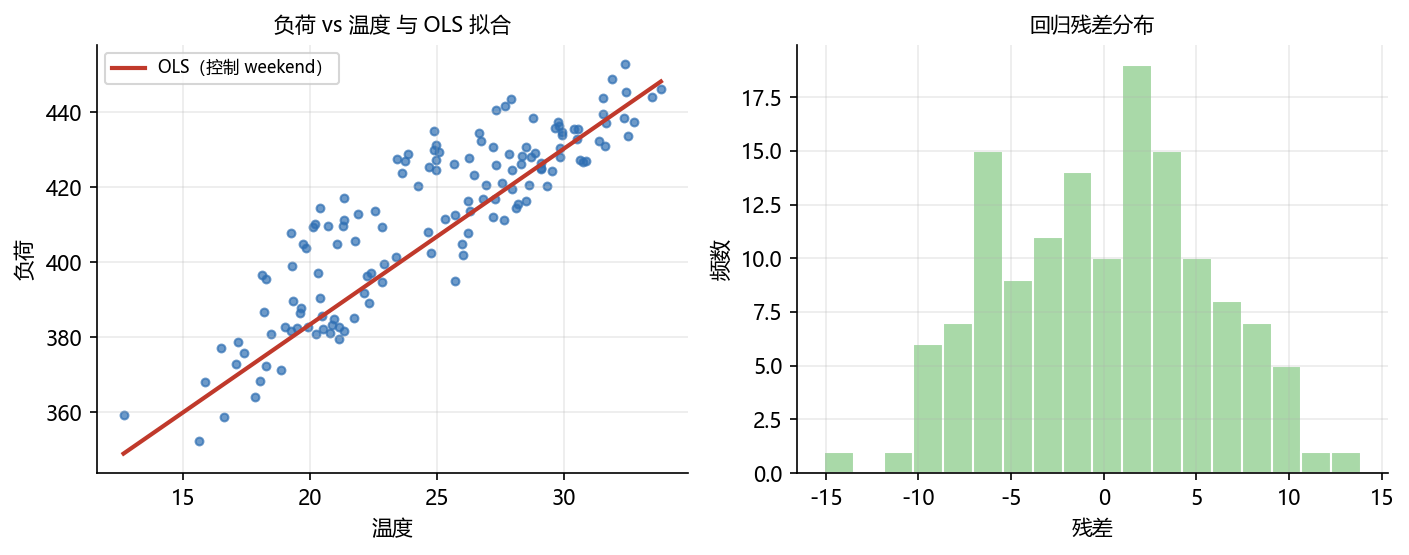
\includegraphics[keepaspectratio,alt={回归诊断：负荷-温度散点与残差分布}]{figures/07-statsmodels/case_regression_diag.png}}
\caption{回归诊断：负荷-温度散点与残差分布}
\end{figure}

\subsection{第 3 步：时间序列分解 + ARIMA
预测}\label{ux7b2c-3-ux6b65ux65f6ux95f4ux5e8fux5217ux5206ux89e3-arima-ux9884ux6d4b}

对负荷序列做周季节性（period=7）加法分解，再用 ARIMA(1,1,1) 预测未来 7
天：

\begin{Shaded}
\begin{Highlighting}[]
\NormalTok{load\_s }\OperatorTok{=}\NormalTok{ pd.Series(dfc[}\StringTok{\textquotesingle{}load\textquotesingle{}}\NormalTok{].values, index}\OperatorTok{=}\NormalTok{date)}
\NormalTok{res }\OperatorTok{=}\NormalTok{ seasonal\_decompose(load\_s, model}\OperatorTok{=}\StringTok{\textquotesingle{}additive\textquotesingle{}}\NormalTok{, period}\OperatorTok{=}\DecValTok{7}\NormalTok{)}
\BuiltInTok{print}\NormalTok{(}\StringTok{"残差标准差 ="}\NormalTok{, }\BuiltInTok{round}\NormalTok{(res.resid.std(), }\DecValTok{3}\NormalTok{))}

\NormalTok{mod }\OperatorTok{=}\NormalTok{ ARIMA(load\_s, order}\OperatorTok{=}\NormalTok{(}\DecValTok{1}\NormalTok{, }\DecValTok{1}\NormalTok{, }\DecValTok{1}\NormalTok{)).fit()}
\NormalTok{fc }\OperatorTok{=}\NormalTok{ mod.forecast(steps}\OperatorTok{=}\DecValTok{7}\NormalTok{)}
\BuiltInTok{print}\NormalTok{(}\StringTok{"未来 7 天预测:"}\NormalTok{, np.}\BuiltInTok{round}\NormalTok{(fc.values, }\DecValTok{2}\NormalTok{))}
\BuiltInTok{print}\NormalTok{(}\StringTok{"AR 系数:"}\NormalTok{, mod.arparams, }\StringTok{" MA 系数:"}\NormalTok{, mod.maparams)}
\end{Highlighting}
\end{Shaded}

运行结果：

\begin{Shaded}
\begin{Highlighting}[]
\NormalTok{残差标准差 = 6.587}
\NormalTok{未来 7 天预测: [413.05 412.49 412.6  412.58 412.58 412.58 412.58]}
\NormalTok{AR 系数: [{-}0.19566366] MA 系数: [0.50904563]}
\end{Highlighting}
\end{Shaded}

\begin{figure}
\centering
\pandocbounded{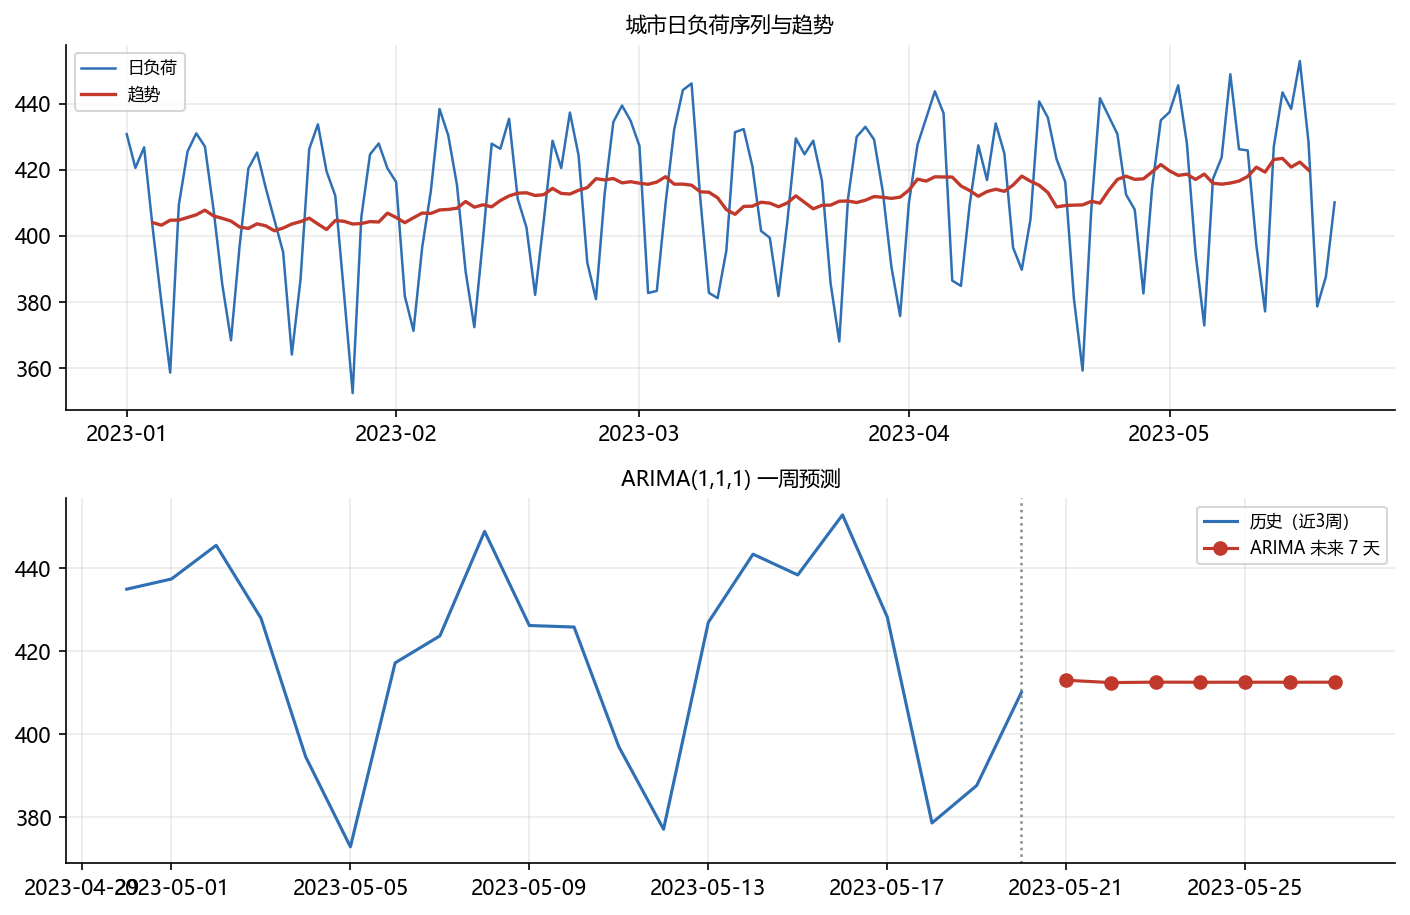
\includegraphics[keepaspectratio,alt={时间序列：序列趋势与 ARIMA 一周预测}]{figures/07-statsmodels/case_ts_forecast.png}}
\caption{时间序列：序列趋势与 ARIMA 一周预测}
\end{figure}

\textbf{结论}：

\begin{itemize}
\tightlist
\item
  残差标准差约 6.6，说明模型已抓住大部分趋势与季节；
\item
  ARIMA(1,1,1) 给出的未来 7 天预测稳定在 412.6
  左右（序列已进入较平稳区间）；
\item
  结合第 2
  步：若未来一周气温升高，可直接用回归式估算负荷增量，作为短期调度参考。
\end{itemize}

\subsection{增强：时间序列诊断与预测误差对比}\label{ux589eux5f3aux65f6ux95f4ux5e8fux5217ux8bcaux65adux4e0eux9884ux6d4bux8befux5deeux5bf9ux6bd4}

综合案例不只是``把三个方法跑一遍''，还应该\textbf{检验模型是否值得信任}。下面补两件事：①
对日负荷做 ADF 平稳性检验（定 \texttt{d} 的依据）；② 把前 120
天当训练、后 20 天当测试，分别用 ARIMA
与``温度+周末''回归做预测，用测试集 RMSE 比较谁更准。

\begin{Shaded}
\begin{Highlighting}[]
\ImportTok{import}\NormalTok{ numpy }\ImportTok{as}\NormalTok{ np}
\ImportTok{import}\NormalTok{ pandas }\ImportTok{as}\NormalTok{ pd}
\ImportTok{import}\NormalTok{ statsmodels.api }\ImportTok{as}\NormalTok{ sm}
\ImportTok{from}\NormalTok{ statsmodels.tsa.stattools }\ImportTok{import}\NormalTok{ adfuller}
\ImportTok{from}\NormalTok{ statsmodels.tsa.arima.model }\ImportTok{import}\NormalTok{ ARIMA}

\NormalTok{rng }\OperatorTok{=}\NormalTok{ np.random.default\_rng(}\DecValTok{7}\NormalTok{)}
\NormalTok{m }\OperatorTok{=} \DecValTok{140}
\NormalTok{date }\OperatorTok{=}\NormalTok{ pd.date\_range(}\StringTok{\textquotesingle{}2023{-}01{-}01\textquotesingle{}}\NormalTok{, periods}\OperatorTok{=}\NormalTok{m, freq}\OperatorTok{=}\StringTok{\textquotesingle{}D\textquotesingle{}}\NormalTok{)}
\NormalTok{trendc }\OperatorTok{=}\NormalTok{ np.linspace(}\DecValTok{0}\NormalTok{, }\DecValTok{15}\NormalTok{, m)}
\NormalTok{seasonc }\OperatorTok{=} \DecValTok{5}\OperatorTok{*}\NormalTok{np.sin(}\DecValTok{2}\OperatorTok{*}\NormalTok{np.pi}\OperatorTok{*}\NormalTok{np.arange(m)}\OperatorTok{/}\DecValTok{7}\NormalTok{) }\OperatorTok{+} \DecValTok{2}\OperatorTok{*}\NormalTok{np.cos(}\DecValTok{2}\OperatorTok{*}\NormalTok{np.pi}\OperatorTok{*}\NormalTok{np.arange(m)}\OperatorTok{/}\DecValTok{7}\NormalTok{)}
\NormalTok{noisec }\OperatorTok{=}\NormalTok{ rng.normal(}\DecValTok{0}\NormalTok{, }\DecValTok{3}\NormalTok{, m)}
\NormalTok{weekend }\OperatorTok{=}\NormalTok{ (date.dayofweek }\OperatorTok{\textgreater{}=} \DecValTok{5}\NormalTok{).astype(}\BuiltInTok{int}\NormalTok{)}
\NormalTok{temp }\OperatorTok{=} \DecValTok{25} \OperatorTok{+} \DecValTok{6}\OperatorTok{*}\NormalTok{np.sin(}\DecValTok{2}\OperatorTok{*}\NormalTok{np.pi}\OperatorTok{*}\NormalTok{np.arange(m)}\OperatorTok{/}\DecValTok{7}\NormalTok{) }\OperatorTok{+}\NormalTok{ rng.normal(}\DecValTok{0}\NormalTok{, }\DecValTok{2}\NormalTok{, m)}
\NormalTok{load }\OperatorTok{=} \DecValTok{300} \OperatorTok{+} \DecValTok{4}\OperatorTok{*}\NormalTok{temp }\OperatorTok{+} \DecValTok{20}\OperatorTok{*}\NormalTok{weekend }\OperatorTok{+}\NormalTok{ trendc }\OperatorTok{+}\NormalTok{ seasonc }\OperatorTok{+}\NormalTok{ noisec}
\NormalTok{dfc }\OperatorTok{=}\NormalTok{ pd.DataFrame(\{}\StringTok{\textquotesingle{}date\textquotesingle{}}\NormalTok{: date, }\StringTok{\textquotesingle{}load\textquotesingle{}}\NormalTok{: load, }\StringTok{\textquotesingle{}weekend\textquotesingle{}}\NormalTok{: weekend, }\StringTok{\textquotesingle{}temp\textquotesingle{}}\NormalTok{: temp\})}
\NormalTok{load\_s }\OperatorTok{=}\NormalTok{ pd.Series(dfc[}\StringTok{\textquotesingle{}load\textquotesingle{}}\NormalTok{].values, index}\OperatorTok{=}\NormalTok{date)}

\NormalTok{adf\_p }\OperatorTok{=}\NormalTok{ adfuller(load\_s)[}\DecValTok{1}\NormalTok{]}
\BuiltInTok{print}\NormalTok{(}\StringTok{\textquotesingle{}load ADF p = }\SpecialCharTok{\%.3g}\StringTok{\textquotesingle{}} \OperatorTok{\%}\NormalTok{ adf\_p)}

\NormalTok{tr }\OperatorTok{=}\NormalTok{ load\_s.iloc[:}\DecValTok{120}\NormalTok{]}
\NormalTok{te }\OperatorTok{=}\NormalTok{ load\_s.iloc[}\DecValTok{120}\NormalTok{:]}
\NormalTok{mtr }\OperatorTok{=}\NormalTok{ ARIMA(tr, order}\OperatorTok{=}\NormalTok{(}\DecValTok{1}\NormalTok{, }\DecValTok{1}\NormalTok{, }\DecValTok{1}\NormalTok{)).fit()}
\NormalTok{fc }\OperatorTok{=}\NormalTok{ mtr.forecast(steps}\OperatorTok{=}\BuiltInTok{len}\NormalTok{(te))}
\NormalTok{rmse\_arima }\OperatorTok{=} \BuiltInTok{float}\NormalTok{(np.sqrt(np.mean((te.values }\OperatorTok{{-}}\NormalTok{ fc.values)}\OperatorTok{**}\DecValTok{2}\NormalTok{)))}
\BuiltInTok{print}\NormalTok{(}\StringTok{\textquotesingle{}ARIMA(1,1,1) test RMSE = }\SpecialCharTok{\%.3f}\StringTok{\textquotesingle{}} \OperatorTok{\%}\NormalTok{ rmse\_arima)}

\NormalTok{x\_tr }\OperatorTok{=}\NormalTok{ dfc[[}\StringTok{\textquotesingle{}temp\textquotesingle{}}\NormalTok{, }\StringTok{\textquotesingle{}weekend\textquotesingle{}}\NormalTok{]].iloc[:}\DecValTok{120}\NormalTok{]}
\NormalTok{y\_tr }\OperatorTok{=}\NormalTok{ dfc[}\StringTok{\textquotesingle{}load\textquotesingle{}}\NormalTok{].iloc[:}\DecValTok{120}\NormalTok{]}
\NormalTok{x\_te }\OperatorTok{=}\NormalTok{ dfc[[}\StringTok{\textquotesingle{}temp\textquotesingle{}}\NormalTok{, }\StringTok{\textquotesingle{}weekend\textquotesingle{}}\NormalTok{]].iloc[}\DecValTok{120}\NormalTok{:]}
\NormalTok{y\_te }\OperatorTok{=}\NormalTok{ dfc[}\StringTok{\textquotesingle{}load\textquotesingle{}}\NormalTok{].iloc[}\DecValTok{120}\NormalTok{:]}
\NormalTok{mreg }\OperatorTok{=}\NormalTok{ sm.OLS(y\_tr, sm.add\_constant(x\_tr)).fit()}
\NormalTok{pred\_reg }\OperatorTok{=}\NormalTok{ mreg.predict(sm.add\_constant(x\_te))}
\NormalTok{rmse\_reg }\OperatorTok{=} \BuiltInTok{float}\NormalTok{(np.sqrt(np.mean((y\_te.values }\OperatorTok{{-}}\NormalTok{ pred\_reg.values)}\OperatorTok{**}\DecValTok{2}\NormalTok{)))}
\BuiltInTok{print}\NormalTok{(}\StringTok{\textquotesingle{}OLS(temp,weekend) test RMSE = }\SpecialCharTok{\%.3f}\StringTok{\textquotesingle{}} \OperatorTok{\%}\NormalTok{ rmse\_reg)}
\end{Highlighting}
\end{Shaded}

\subsubsection{运行结果（已运行核验）}\label{ux8fd0ux884cux7ed3ux679cux5df2ux8fd0ux884cux6838ux9a8c-29}

\begin{Shaded}
\begin{Highlighting}[]
\NormalTok{load ADF p = 0.774}
\NormalTok{ARIMA(1,1,1) test RMSE = 29.412}
\NormalTok{OLS(temp,weekend) test RMSE = 7.808}
\end{Highlighting}
\end{Shaded}

\textbf{解读}：

\begin{itemize}
\tightlist
\item
  \texttt{load\ ADF\ p\ =\ 0.774\ \textgreater{}\ 0.05}：日负荷序列非平稳，所以第
  3 步用 \texttt{ARIMA(...,d=1)} 是合理的；若想用 \texttt{SARIMAX}
  含外生温度，也应先差分。
\item
  测试集 RMSE 上，\texttt{OLS(temp,\ weekend)} 为
  \textbf{7.81}，明显优于 \texttt{ARIMA(1,1,1)} 的
  \textbf{29.41}：因为负荷主要受温度与周末影响，回归能``用上外生变量''，而纯
  ARIMA 只能靠历史轨迹外推。
\item
  这不代表 ARIMA
  没用：若没有温度等外生变量，或只关心短期的纯时间形态，ARIMA
  是更好的基线；更复杂的 \texttt{SARIMAX}（把 \texttt{temp}
  当外生变量）通常能进一步压小 RMSE。
\end{itemize}

\subsection{本章小结}\label{ux672cux7ae0ux5c0fux7ed3}

{\def\LTcaptype{none} % do not increment counter
\begin{longtable}[]{@{}ll@{}}
\toprule\noalign{}
方法 & 结论 \\
\midrule\noalign{}
\endhead
\bottomrule\noalign{}
\endlastfoot
ANOVA & 周末负荷显著高于工作日（P=0.029） \\
OLS & 温度每 +1°C 负荷 +4.69；周末 +21.0；R²=0.94 \\
分解+ARIMA & 残差 σ≈6.6；未来 7 天预测约 412.6 \\
\end{longtable}
}

\textbf{拓展任务}：

\begin{enumerate}
\def\labelenumi{\arabic{enumi}.}
\tightlist
\item
  用 typ=3 重跑方差分析，比较结果；
\item
  在回归中加入 temp*weekend 交互项，判断周末的温度效应是否不同；
\item
  用 SARIMAX（含外生温度变量）替代 ARIMA，比较预测误差；
\item
  将前 120 天作为训练、后 20 天作为测试，用 RMSE 评估不同模型。
\end{enumerate}

\section{04
常见误区与技巧}\label{ux5e38ux89c1ux8befux533aux4e0eux6280ux5de7-6}

\begin{quote}
本章为新增``查漏补缺''页：把 statsmodels
使用中最容易踩的坑集中列出，并给出正确写法、性能与调试技巧。
\end{quote}

\subsection{1.
高频误区速查表}\label{ux9ad8ux9891ux8befux533aux901fux67e5ux8868-6}

{\def\LTcaptype{none} % do not increment counter
\begin{longtable}[]{@{}
  >{\raggedright\arraybackslash}p{(\linewidth - 6\tabcolsep) * \real{0.2500}}
  >{\raggedright\arraybackslash}p{(\linewidth - 6\tabcolsep) * \real{0.2500}}
  >{\raggedright\arraybackslash}p{(\linewidth - 6\tabcolsep) * \real{0.2500}}
  >{\raggedright\arraybackslash}p{(\linewidth - 6\tabcolsep) * \real{0.2500}}@{}}
\toprule\noalign{}
\begin{minipage}[b]{\linewidth}\raggedright
\#
\end{minipage} & \begin{minipage}[b]{\linewidth}\raggedright
误区 / 错误写法
\end{minipage} & \begin{minipage}[b]{\linewidth}\raggedright
正确做法
\end{minipage} & \begin{minipage}[b]{\linewidth}\raggedright
原因
\end{minipage} \\
\midrule\noalign{}
\endhead
\bottomrule\noalign{}
\endlastfoot
1 & sm.OLS(y, X) 直接用原始 X & X = sm.add\_constant(X) & OLS
默认不自动加截距 \\
2 & 公式里 y \textasciitilde{} group & y \textasciitilde{} C(group) &
分类变量需转成哑变量 \\
3 & y \textasciitilde{} x1 * x2 当``乘法项'' & y \textasciitilde{} x1 +
I(x1*x2) 或 y \textasciitilde{} x1 + x2 + x1:x2 & 公式里 *
表示主效应+交互 \\
4 & 用 predict(X\_new) 预测 & 预测前也要 sm.add\_constant(X\_new) &
训练/预测设计矩阵必须一致 \\
5 & 把 GLM predict 当 0/1 & 需要 (p \textgreater{} thr).astype(int) &
默认返回到概率 p，不是类别 \\
6 & 对非平稳序列直接 ARIMA & 先 adfuller，必要时差分 &
非平稳易``伪回归'' \\
7 & seasonal\_decompose 不设 period & 日数据设 7、月数据设 12 &
否则季节期抓不到 \\
8 & 忘差分后 dropna() & ts.diff().dropna() & 差分首元素为 NaN \\
9 & 只看 R² 不看诊断 & 同时看 summary() 的 F、P、JB、Durbin-Watson & R²
高可能只是表面拟合 \\
10 & 用 np.linalg.lstsq 替代 OLS 推断 & 需要 P 值/置信区间用 sm.OLS &
lstsq 只给系数，不给推断 \\
11 & 用 anova\_lm 传原始数组 & 传 ols(\ldots).fit() 的结果 & anova\_lm
需要回归结果对象 \\
12 & 混淆 params 与 bse & 系数看 params，精度看 bse/P 值 & params
只是点估计 \\
\end{longtable}
}

\subsection{2. 原理级难点}\label{ux539fux7406ux7ea7ux96beux70b9}

\subsubsection{2.1
为什么必须加常数列}\label{ux4e3aux4ec0ux4e48ux5fc5ux987bux52a0ux5e38ux6570ux5217}

OLS 的模型是 \(y = X\beta + \varepsilon\)。若不手动加一列全
1，模型里就没有截距项，相当于强制过原点。公式 API 会自动加
Intercept，而数组 API 需要你显式 sm.add\_constant。

\subsubsection{2.2 C()、I()、* 的区别}\label{ci-ux7684ux533aux522b}

ols 用的公式语法来自 patsy：

\begin{itemize}
\tightlist
\item
  C(x)：把数值列当分类变量；
\item
  I(x**2)：对数值列做数学变换（I 包裹）；
\item
  x1*x2：展开为主效应+交互；x1:x2 只写交互；x1+x2 只加主效应。
\end{itemize}

\subsubsection{2.3 predict
返回什么}\label{predict-ux8fd4ux56deux4ec0ux4e48}

默认 predict 返回\textbf{线性预测值}（对 GLM 是 logit
的线性部分），需要加参数 linear=False 或直接用概率。对
OLS，两者一致。对二分类 GLM，想得到概率且区分清楚，建议用
model.predict(X)（默认即概率），再用阈值分类。

\subsubsection{2.4 summary()
里关键字段}\label{summary-ux91ccux5173ux952eux5b57ux6bb5}

{\def\LTcaptype{none} % do not increment counter
\begin{longtable}[]{@{}
  >{\raggedright\arraybackslash}p{(\linewidth - 4\tabcolsep) * \real{0.3333}}
  >{\raggedright\arraybackslash}p{(\linewidth - 4\tabcolsep) * \real{0.3333}}
  >{\raggedright\arraybackslash}p{(\linewidth - 4\tabcolsep) * \real{0.3333}}@{}}
\toprule\noalign{}
\begin{minipage}[b]{\linewidth}\raggedright
字段
\end{minipage} & \begin{minipage}[b]{\linewidth}\raggedright
含义
\end{minipage} & \begin{minipage}[b]{\linewidth}\raggedright
关注点
\end{minipage} \\
\midrule\noalign{}
\endhead
\bottomrule\noalign{}
\endlastfoot
coef & 系数估计 & 解释``每单位变化'' \\
std err & 标准误 & 越小越稳 \\
t / P\textgreater{} & t & \\
{[}0.025, 0.975{]} & 95\% 置信区间 & 含 0 一般说明不显著 \\
R² / Adj. R² & 拟合优度 & Adj. R² 更能防过拟合 \\
F / Prob(F) & 整体显著性 & 模型整体是否有解释力 \\
Jarque-Bera / Prob(JB) & 残差正态性 & Prob(JB)\textgreater0.05 可接受 \\
Durbin-Watson & 残差自相关 & 接近 2 好 \\
\end{longtable}
}

\subsection{3. 性能技巧}\label{ux6027ux80fdux6280ux5de7-5}

\begin{itemize}
\tightlist
\item
  \textbf{先聚合再建模}：对大数据，先用 groupby
  聚合或抽样，减少矩阵规模；
\item
  \textbf{避免频繁 summary()}：大模型渲染完整摘要会慢，调试时用
  params、bse、rsquared 等属性；
\item
  \textbf{OLS 可用 np.linalg.lstsq 快速求解}，但推断请回落 statsmodels；
\item
  \textbf{GLM 拟合用 fit(maxiter=\ldots) 控制迭代}，必要时增加 maxiter；
\item
  \textbf{时间序列建模}：ARIMA 用 model.fit(method=`lbfgs') 或
  disp=False 减少输出，提升速度；
\item
  \textbf{大数据回归}：考虑 GD/IRLS（fit\_regularized）或改用
  scikit-learn。
\end{itemize}

\subsection{4. 调试建议}\label{ux8c03ux8bd5ux5efaux8bae-6}

\begin{enumerate}
\def\labelenumi{\arabic{enumi}.}
\tightlist
\item
  先打印 type(df)、df.shape、df.dtypes，确认数据已正确进入 DataFrame；
\item
  确认因变量 y 是一维 Series/array，自变量 X 是二维；（X.shape）
\item
  用 sm.add\_constant 后立即检查列名是否含 const；
\item
  用 help(model)、dir(model)
  查看可用属性（params、bse、pvalues、conf\_int）；
\item
  随机/拟合问题\textbf{固定种子}
  np.random.default\_rng(seed)，便于复现；
\item
  用 df.isna().sum()、np.isinf 检查缺失与异常值；
\item
  公式写错时，把 data=df 换成 data=df{[}{[}`x',`y'{]}{]} 或打印
  df.head() 排除列名问题。
\end{enumerate}

\subsection{5. 本章自测清单}\label{ux672cux7ae0ux81eaux6d4bux6e05ux5355}

\begin{itemize}
\tightlist
\item[$\square$]
  能区分 sm.OLS 数组接口与 ols 公式接口；
\item[$\square$]
  能在 summary() 中找到并解释 R²、F、P 值、JB 统计量；
\item[$\square$]
  会做单因素方差分析并读 F/P 值；
\item[$\square$]
  会用 GLM(Binomial) 拟合并得到概率；
\item[$\square$]
  会对时间序列分解并解释趋势/季节/残差；
\item[$\square$]
  会用 adfuller 判断平稳性；
\item[$\square$]
  会用 ARIMA 拟合与预测并画图。
\end{itemize}

\subsection{6. 延伸阅读}\label{ux5ef6ux4f38ux9605ux8bfb-33}

\begin{itemize}
\tightlist
\item
  statsmodels 官方``Statistical
  Models''教学：\href{https://www.statsmodels.org/stable/user-guide.html}{链接}
\item
  Statsmodels
  官方示例集：\href{https://www.statsmodels.org/stable/examples/index.html}{链接}
\item
  patsy
  公式语法：\href{https://patsy.readthedocs.io/en/latest/formulas.html}{链接}
\end{itemize}

\newpage

%% 由 build/emit_tex.py 生成（生成物，勿手改）；定制请放 user_style.tex / user_meta.yaml
\chapter{Sklearn及其基本使用}\label{sklearnux53caux5176ux57faux672cux4f7fux7528}

\section{01
数据集的预处理}\label{ux6570ux636eux96c6ux7684ux9884ux5904ux7406}

\begin{quote}
本节是从``原始数据''到``可训练数据''的第一步：特征编码、特征缩放、数据集切分、交叉验证与特征选择。所有代码在
sklearn 1.6.1、Python 3.13 下运行验证。
\end{quote}

\subsection{本节目标}\label{ux672cux8282ux76eeux6807-21}

\begin{enumerate}
\def\labelenumi{\arabic{enumi}.}
\tightlist
\item
  会用 \texttt{OneHotEncoder} / \texttt{LabelEncoder}
  处理分类特征，并说清两者适用场景。
\item
  会用 \texttt{StandardScaler} / \texttt{MinMaxScaler} 缩放连续特征。
\item
  会用 \texttt{train\_test\_split} 切分数据，并用
  \texttt{cross\_val\_score} / \texttt{LeaveOneOut} 做交叉验证。
\item
  会用
  \texttt{VarianceThreshold}、\texttt{SelectKBest}、\texttt{RFE}、\texttt{Lasso}、\texttt{SelectFromModel}
  做特征选择。
\item
  理解预处理必须放在 Pipeline 中，避免数据泄漏。
\end{enumerate}

\subsection{先修}\label{ux5148ux4fee-21}

\begin{itemize}
\tightlist
\item
  NumPy 数组操作、Pandas 基本用法（第 1、4 章）。
\item
  了解``均值/方差/相关系数''与``特征量纲''概念。
\end{itemize}

\subsection{官方文档 /
参考入口}\label{ux5b98ux65b9ux6587ux6863-ux53c2ux8003ux5165ux53e3-7}

\begin{itemize}
\tightlist
\item
  sklearn
  预处理：https://scikit-learn.org/stable/modules/preprocessing.html
\item
  sklearn
  模型选择：https://scikit-learn.org/stable/modules/cross\_validation.html
\item
  sklearn
  特征选择：https://scikit-learn.org/stable/modules/feature\_selection.html
\item
  sklearn 数据分割
  API：https://scikit-learn.org/stable/modules/generated/sklearn.model\_selection.train\_test\_split.html
\end{itemize}

\subsection{正文}\label{ux6b63ux6587}

\subsubsection{1.
特征编码：把``文字''变成``数字''}\label{ux7279ux5f81ux7f16ux7801ux628aux6587ux5b57ux53d8ux6210ux6570ux5b57}

大多数 sklearn 模型只能吃数值矩阵。对待分类特征，有两种常见编码。

\paragraph{1.1
独热编码（OneHotEncoder）}\label{ux72ecux70edux7f16ux7801onehotencoder}

把每个类别展开成一位为 1、其余为 0 的向量。默认输出稀疏矩阵，用
\texttt{sparse\_output=False} 得到稠密数组。

\begin{Shaded}
\begin{Highlighting}[]
\ImportTok{import}\NormalTok{ numpy }\ImportTok{as}\NormalTok{ np}
\ImportTok{from}\NormalTok{ sklearn.preprocessing }\ImportTok{import}\NormalTok{ OneHotEncoder}

\NormalTok{data }\OperatorTok{=}\NormalTok{ np.array([[}\StringTok{\textquotesingle{}male\textquotesingle{}}\NormalTok{], [}\StringTok{\textquotesingle{}female\textquotesingle{}}\NormalTok{], [}\StringTok{\textquotesingle{}male\textquotesingle{}}\NormalTok{], [}\StringTok{\textquotesingle{}female\textquotesingle{}}\NormalTok{]])}
\NormalTok{encoder }\OperatorTok{=}\NormalTok{ OneHotEncoder(sparse\_output}\OperatorTok{=}\VariableTok{False}\NormalTok{)}
\NormalTok{encoded }\OperatorTok{=}\NormalTok{ encoder.fit\_transform(data)}
\BuiltInTok{print}\NormalTok{(}\StringTok{"categories\_:"}\NormalTok{, encoder.categories\_)}
\BuiltInTok{print}\NormalTok{(}\StringTok{"shape:"}\NormalTok{, encoded.shape)}
\BuiltInTok{print}\NormalTok{(}\StringTok{"特征名:"}\NormalTok{, encoder.get\_feature\_names\_out())}
\BuiltInTok{print}\NormalTok{(encoded)}
\end{Highlighting}
\end{Shaded}

\begin{Shaded}
\begin{Highlighting}[]
\NormalTok{categories\_: [array([\textquotesingle{}female\textquotesingle{}, \textquotesingle{}male\textquotesingle{}], dtype=\textquotesingle{}\textless{}U6\textquotesingle{})]}
\NormalTok{shape: (4, 2)}
\NormalTok{特征名: [\textquotesingle{}x0\_female\textquotesingle{} \textquotesingle{}x0\_male\textquotesingle{}]}
\NormalTok{[[0. 1.]}
\NormalTok{ [1. 0.]}
\NormalTok{ [0. 1.]}
\NormalTok{ [1. 0.]]}
\end{Highlighting}
\end{Shaded}

\begin{quote}
注意：\texttt{male} 被编码为 \texttt{{[}0,1{]}}（因为
\texttt{categories\_} 按字母序把 \texttt{female} 排在 0
列、\texttt{male} 排 1
列）。独热编码没有``谁大谁小''的含义，适合无序类别。
\end{quote}

\paragraph{1.2
标签编码（LabelEncoder）}\label{ux6807ux7b7eux7f16ux7801labelencoder}

把每个类别映射成 0、1、2
等整数。它暗示类别之间有顺序，对无序类别（如颜色、性别）通常不合适。

\begin{Shaded}
\begin{Highlighting}[]
\ImportTok{from}\NormalTok{ sklearn.preprocessing }\ImportTok{import}\NormalTok{ LabelEncoder}

\NormalTok{labels }\OperatorTok{=}\NormalTok{ [}\StringTok{\textquotesingle{}male\textquotesingle{}}\NormalTok{, }\StringTok{\textquotesingle{}female\textquotesingle{}}\NormalTok{, }\StringTok{\textquotesingle{}male\textquotesingle{}}\NormalTok{, }\StringTok{\textquotesingle{}female\textquotesingle{}}\NormalTok{]}
\NormalTok{le }\OperatorTok{=}\NormalTok{ LabelEncoder().fit(labels)}
\BuiltInTok{print}\NormalTok{(}\StringTok{"classes\_:"}\NormalTok{, le.classes\_)}
\BuiltInTok{print}\NormalTok{(}\StringTok{"transform:"}\NormalTok{, le.transform(labels))}
\end{Highlighting}
\end{Shaded}

\begin{Shaded}
\begin{Highlighting}[]
\NormalTok{classes\_: [\textquotesingle{}female\textquotesingle{} \textquotesingle{}male\textquotesingle{}]}
\NormalTok{transform: [1 0 1 0]}
\end{Highlighting}
\end{Shaded}

\begin{quote}
若类别本身有序（如 \texttt{小/中/大}），可改用 \texttt{OrdinalEncoder}
并显式指定 \texttt{categories}；若只是把字符串标签喂给分类器，常用
\texttt{LabelEncoder} 只看目标 y，而特征 x 的分类列建议用
\texttt{OneHotEncoder} 或 \texttt{OrdinalEncoder}。
\end{quote}

\subsubsection{2.
特征缩放：把量纲拉平}\label{ux7279ux5f81ux7f29ux653eux628aux91cfux7eb2ux62c9ux5e73}

当各列量纲差别很大（比如一列在 0\textasciitilde1，另一列在 10\^{}4
量级）时，距离类算法（KNN、SVM、KMeans、PCA）会被大方差特征主导，因此需要缩放。

\paragraph{2.1
标准化（StandardScaler）}\label{ux6807ux51c6ux5316standardscaler}

\texttt{x\textquotesingle{}\ =\ (x\ -\ mean)\ /\ std}，使每列均值
0、标准差 1。

\begin{Shaded}
\begin{Highlighting}[]
\ImportTok{import}\NormalTok{ numpy }\ImportTok{as}\NormalTok{ np}
\ImportTok{from}\NormalTok{ sklearn.preprocessing }\ImportTok{import}\NormalTok{ StandardScaler}

\NormalTok{X }\OperatorTok{=}\NormalTok{ np.array([[}\DecValTok{1}\NormalTok{, }\DecValTok{2}\NormalTok{], [}\DecValTok{3}\NormalTok{, }\DecValTok{4}\NormalTok{], [}\DecValTok{5}\NormalTok{, }\DecValTok{6}\NormalTok{]])}
\NormalTok{ss }\OperatorTok{=}\NormalTok{ StandardScaler().fit(X)}
\BuiltInTok{print}\NormalTok{(}\StringTok{"mean\_:"}\NormalTok{, ss.mean\_, }\StringTok{"scale\_:"}\NormalTok{, np.}\BuiltInTok{round}\NormalTok{(ss.scale\_, }\DecValTok{6}\NormalTok{))}
\BuiltInTok{print}\NormalTok{(ss.transform(X))}
\end{Highlighting}
\end{Shaded}

\begin{Shaded}
\begin{Highlighting}[]
\NormalTok{mean\_: [3. 4.] scale\_: [1.632993 1.632993]}
\NormalTok{[[{-}1.22474487 {-}1.22474487]}
\NormalTok{ [ 0.          0.        ]}
\NormalTok{ [ 1.22474487  1.22474487]]}
\end{Highlighting}
\end{Shaded}

\paragraph{2.2
归一化（MinMaxScaler）}\label{ux5f52ux4e00ux5316minmaxscaler}

把每列压缩到 \texttt{{[}0,\ 1{]}}（或其他 \texttt{feature\_range}）。

\begin{Shaded}
\begin{Highlighting}[]
\ImportTok{from}\NormalTok{ sklearn.preprocessing }\ImportTok{import}\NormalTok{ MinMaxScaler}

\NormalTok{mm }\OperatorTok{=}\NormalTok{ MinMaxScaler().fit(X)}
\BuiltInTok{print}\NormalTok{(}\StringTok{"data\_min\_:"}\NormalTok{, mm.data\_min\_, }\StringTok{"data\_max\_:"}\NormalTok{, mm.data\_max\_)}
\BuiltInTok{print}\NormalTok{(mm.transform(X))}
\end{Highlighting}
\end{Shaded}

\begin{Shaded}
\begin{Highlighting}[]
\NormalTok{data\_min\_: [1. 2.] data\_max\_: [5. 6.]}
\NormalTok{[[0.  0. ]}
\NormalTok{ [0.5 0.5]}
\NormalTok{ [1.  1. ]]}
\end{Highlighting}
\end{Shaded}

\begin{quote}
标准化对异常值更稳健（用均值/标准差），归一化把数据严格限制到区间。若有人告诉你``某个算法必须归一化''，指的是这两者之一；具体选哪个要看数据分布与模型（树模型一般不需要缩放）。
\end{quote}

\subsubsection{3.
数据集切分与交叉验证}\label{ux6570ux636eux96c6ux5207ux5206ux4e0eux4ea4ux53c9ux9a8cux8bc1}

\paragraph{3.1 train\_test\_split}\label{train_test_split}

\begin{Shaded}
\begin{Highlighting}[]
\ImportTok{from}\NormalTok{ sklearn.model\_selection }\ImportTok{import}\NormalTok{ train\_test\_split}
\ImportTok{from}\NormalTok{ sklearn.datasets }\ImportTok{import}\NormalTok{ load\_iris}

\NormalTok{iris }\OperatorTok{=}\NormalTok{ load\_iris()}\OperatorTok{;}\NormalTok{ X, y }\OperatorTok{=}\NormalTok{ iris.data, iris.target}
\NormalTok{Xtr, Xte, ytr, yte }\OperatorTok{=}\NormalTok{ train\_test\_split(X, y, test\_size}\OperatorTok{=}\FloatTok{0.3}\NormalTok{, random\_state}\OperatorTok{=}\DecValTok{42}\NormalTok{, stratify}\OperatorTok{=}\NormalTok{y)}
\BuiltInTok{print}\NormalTok{(}\StringTok{"train shape:"}\NormalTok{, Xtr.shape, }\StringTok{"test shape:"}\NormalTok{, Xte.shape)}
\BuiltInTok{print}\NormalTok{(}\StringTok{"测试集各类数量:"}\NormalTok{, np.unique(yte, return\_counts}\OperatorTok{=}\VariableTok{True}\NormalTok{))}
\end{Highlighting}
\end{Shaded}

\begin{Shaded}
\begin{Highlighting}[]
\NormalTok{train shape: (105, 4) test shape: (45, 4)}
\NormalTok{测试集各类数量: (array([0, 1, 2]), array([15, 15, 15]))}
\end{Highlighting}
\end{Shaded}

\begin{quote}
\texttt{stratify=y}
让训练/测试集各类比例一致（对分类很重要）；\texttt{random\_state=42}
保证可复现。
\end{quote}

\paragraph{3.2 K
折交叉验证（cross\_val\_score）}\label{k-ux6298ux4ea4ux53c9ux9a8cux8bc1cross_val_score}

把数据切成 K 份，轮流用 K-1 份训练、1 份测试，最后平均各折分数。

\begin{Shaded}
\begin{Highlighting}[]
\ImportTok{from}\NormalTok{ sklearn.linear\_model }\ImportTok{import}\NormalTok{ LogisticRegression}
\ImportTok{from}\NormalTok{ sklearn.model\_selection }\ImportTok{import}\NormalTok{ cross\_val\_score}

\NormalTok{model }\OperatorTok{=}\NormalTok{ LogisticRegression(max\_iter}\OperatorTok{=}\DecValTok{1000}\NormalTok{)}
\NormalTok{scores }\OperatorTok{=}\NormalTok{ cross\_val\_score(model, Xtr, ytr, cv}\OperatorTok{=}\DecValTok{5}\NormalTok{)}
\BuiltInTok{print}\NormalTok{(}\StringTok{"各折分数:"}\NormalTok{, np.}\BuiltInTok{round}\NormalTok{(scores, }\DecValTok{4}\NormalTok{))}
\BuiltInTok{print}\NormalTok{(}\StringTok{"平均:"}\NormalTok{, }\BuiltInTok{round}\NormalTok{(scores.mean(), }\DecValTok{4}\NormalTok{))}
\end{Highlighting}
\end{Shaded}

\begin{Shaded}
\begin{Highlighting}[]
\NormalTok{各折分数: [0.9524 0.9524 1.     0.9524 1.    ]}
\NormalTok{平均: 0.9714}
\end{Highlighting}
\end{Shaded}

\begin{quote}
\texttt{cross\_val\_score} 内部会把每个模型 \texttt{fit}
在训练折、\texttt{score} 在验证折，因此它比单次 train/test
更稳健、也更少受随机划分影响。
\end{quote}

\paragraph{3.3
留一交叉验证（LeaveOneOut）}\label{ux7559ux4e00ux4ea4ux53c9ux9a8cux8bc1leaveoneout}

每次只留 1 个样本测试。适合小数据集，但计算量大。

\begin{Shaded}
\begin{Highlighting}[]
\ImportTok{from}\NormalTok{ sklearn.model\_selection }\ImportTok{import}\NormalTok{ LeaveOneOut}

\NormalTok{loo }\OperatorTok{=}\NormalTok{ LeaveOneOut()}
\NormalTok{scores }\OperatorTok{=}\NormalTok{ []}
\ControlFlowTok{for}\NormalTok{ tr, te }\KeywordTok{in}\NormalTok{ loo.split(Xtr[:}\DecValTok{30}\NormalTok{], ytr[:}\DecValTok{30}\NormalTok{]):}
\NormalTok{    m }\OperatorTok{=}\NormalTok{ LogisticRegression(max\_iter}\OperatorTok{=}\DecValTok{1000}\NormalTok{).fit(Xtr[tr], ytr[tr])}
\NormalTok{    scores.append(m.score(Xtr[te], ytr[te]))}
\BuiltInTok{print}\NormalTok{(}\StringTok{"留一法样本数:"}\NormalTok{, }\BuiltInTok{len}\NormalTok{(scores), }\StringTok{"平均:"}\NormalTok{, }\BuiltInTok{round}\NormalTok{(np.mean(scores), }\DecValTok{4}\NormalTok{))}
\end{Highlighting}
\end{Shaded}

\begin{Shaded}
\begin{Highlighting}[]
\NormalTok{留一法样本数: 30 平均: 0.9333}
\end{Highlighting}
\end{Shaded}

\subsubsection{4.
特征选择：保留更少的列}\label{ux7279ux5f81ux9009ux62e9ux4fddux7559ux66f4ux5c11ux7684ux5217}

特征选择从原始列中挑出``最重要''的子集，能降低过拟合、加速训练。

\paragraph{4.1
过滤法：VarianceThreshold（方差阈值）}\label{ux8fc7ux6ee4ux6cd5variancethresholdux65b9ux5deeux9608ux503c}

\begin{Shaded}
\begin{Highlighting}[]
\ImportTok{from}\NormalTok{ sklearn.feature\_selection }\ImportTok{import}\NormalTok{ VarianceThreshold}

\NormalTok{sel }\OperatorTok{=}\NormalTok{ VarianceThreshold(threshold}\OperatorTok{=}\FloatTok{0.8}\NormalTok{)}
\NormalTok{Xv }\OperatorTok{=}\NormalTok{ sel.fit\_transform(X)}
\BuiltInTok{print}\NormalTok{(}\StringTok{"方差:"}\NormalTok{, np.}\BuiltInTok{round}\NormalTok{(sel.variances\_, }\DecValTok{4}\NormalTok{))}
\BuiltInTok{print}\NormalTok{(}\StringTok{"变换后 shape:"}\NormalTok{, Xv.shape)}
\end{Highlighting}
\end{Shaded}

\begin{Shaded}
\begin{Highlighting}[]
\NormalTok{方差: [0.6811 0.1887 3.0955 0.5771]}
\NormalTok{变换后 shape: (150, 1)}
\end{Highlighting}
\end{Shaded}

\begin{quote}
只保留方差 ≥ 0.8 的特征（这里只有第 3
列）。方差小的列信息量低；但注意它只按方差筛，完全不看与 y 的关系。
\end{quote}

\paragraph{4.2 过滤法：SelectKBest +
互信息}\label{ux8fc7ux6ee4ux6cd5selectkbest-ux4e92ux4fe1ux606f}

\begin{Shaded}
\begin{Highlighting}[]
\ImportTok{from}\NormalTok{ sklearn.feature\_selection }\ImportTok{import}\NormalTok{ SelectKBest, mutual\_info\_classif}

\NormalTok{selb }\OperatorTok{=}\NormalTok{ SelectKBest(mutual\_info\_classif, k}\OperatorTok{=}\DecValTok{2}\NormalTok{)}
\NormalTok{Xb }\OperatorTok{=}\NormalTok{ selb.fit\_transform(X, y)}
\BuiltInTok{print}\NormalTok{(}\StringTok{"选中的特征索引:"}\NormalTok{, selb.get\_support(indices}\OperatorTok{=}\VariableTok{True}\NormalTok{))}
\BuiltInTok{print}\NormalTok{(}\StringTok{"各特征互信息:"}\NormalTok{, np.}\BuiltInTok{round}\NormalTok{(selb.scores\_, }\DecValTok{4}\NormalTok{))}
\BuiltInTok{print}\NormalTok{(}\StringTok{"变换后 shape:"}\NormalTok{, Xb.shape)}
\end{Highlighting}
\end{Shaded}

\begin{Shaded}
\begin{Highlighting}[]
\NormalTok{选中的特征索引: [2 3]}
\NormalTok{各特征互信息: [0.494  0.2597 0.9784 0.9804]}
\NormalTok{变换后 shape: (150, 2)}
\end{Highlighting}
\end{Shaded}

\paragraph{4.3
包装法：RFE（递归特征消除）}\label{ux5305ux88c5ux6cd5rfeux9012ux5f52ux7279ux5f81ux6d88ux9664}

\begin{Shaded}
\begin{Highlighting}[]
\ImportTok{from}\NormalTok{ sklearn.linear\_model }\ImportTok{import}\NormalTok{ LogisticRegression}
\ImportTok{from}\NormalTok{ sklearn.feature\_selection }\ImportTok{import}\NormalTok{ RFE}

\NormalTok{est }\OperatorTok{=}\NormalTok{ LogisticRegression(max\_iter}\OperatorTok{=}\DecValTok{1000}\NormalTok{)}
\NormalTok{r }\OperatorTok{=}\NormalTok{ RFE(est, n\_features\_to\_select}\OperatorTok{=}\DecValTok{2}\NormalTok{)}
\NormalTok{Xr }\OperatorTok{=}\NormalTok{ r.fit\_transform(X, y)}
\BuiltInTok{print}\NormalTok{(}\StringTok{"support\_:"}\NormalTok{, r.support\_)}
\BuiltInTok{print}\NormalTok{(}\StringTok{"ranking\_:"}\NormalTok{, r.ranking\_)}
\BuiltInTok{print}\NormalTok{(}\StringTok{"变换后 shape:"}\NormalTok{, Xr.shape)}
\end{Highlighting}
\end{Shaded}

\begin{Shaded}
\begin{Highlighting}[]
\NormalTok{support\_: [False False  True  True]}
\NormalTok{ranking\_: [3 2 1 1]}
\NormalTok{变换后 shape: (150, 2)}
\end{Highlighting}
\end{Shaded}

\paragraph{4.4 嵌入法：Lasso /
SelectFromModel}\label{ux5d4cux5165ux6cd5lasso-selectfrommodel}

Lasso 的 L1 正则会把不重要的系数压到 0；用 \texttt{SelectFromModel}
包一个树模型，可按重要性阈值自动选列。

\begin{Shaded}
\begin{Highlighting}[]
\ImportTok{from}\NormalTok{ sklearn.linear\_model }\ImportTok{import}\NormalTok{ Lasso}

\NormalTok{ls }\OperatorTok{=}\NormalTok{ Lasso(alpha}\OperatorTok{=}\FloatTok{0.1}\NormalTok{).fit(X, y)}
\BuiltInTok{print}\NormalTok{(}\StringTok{"Lasso 系数:"}\NormalTok{, np.}\BuiltInTok{round}\NormalTok{(ls.coef\_, }\DecValTok{6}\NormalTok{))}
\BuiltInTok{print}\NormalTok{(}\StringTok{"非零掩码:"}\NormalTok{, ls.coef\_ }\OperatorTok{!=} \DecValTok{0}\NormalTok{)}
\end{Highlighting}
\end{Shaded}

\begin{Shaded}
\begin{Highlighting}[]
\NormalTok{Lasso 系数: [ 0.       {-}0.        0.408119  0.      ]}
\NormalTok{非零掩码: [False False  True False]}
\end{Highlighting}
\end{Shaded}

\begin{Shaded}
\begin{Highlighting}[]
\ImportTok{from}\NormalTok{ sklearn.ensemble }\ImportTok{import}\NormalTok{ RandomForestClassifier}
\ImportTok{from}\NormalTok{ sklearn.feature\_selection }\ImportTok{import}\NormalTok{ SelectFromModel}

\NormalTok{rf }\OperatorTok{=}\NormalTok{ RandomForestClassifier(n\_estimators}\OperatorTok{=}\DecValTok{10}\NormalTok{, random\_state}\OperatorTok{=}\DecValTok{42}\NormalTok{).fit(X, y)}
\NormalTok{selm }\OperatorTok{=}\NormalTok{ SelectFromModel(rf, prefit}\OperatorTok{=}\VariableTok{True}\NormalTok{, threshold}\OperatorTok{=}\StringTok{\textquotesingle{}mean\textquotesingle{}}\NormalTok{)}
\NormalTok{Xm }\OperatorTok{=}\NormalTok{ selm.transform(X)}
\BuiltInTok{print}\NormalTok{(}\StringTok{"重要性:"}\NormalTok{, np.}\BuiltInTok{round}\NormalTok{(rf.feature\_importances\_, }\DecValTok{4}\NormalTok{), }\StringTok{" 均值:"}\NormalTok{, }\BuiltInTok{round}\NormalTok{(rf.feature\_importances\_.mean(), }\DecValTok{4}\NormalTok{))}
\BuiltInTok{print}\NormalTok{(}\StringTok{"support\_:"}\NormalTok{, selm.get\_support())}
\BuiltInTok{print}\NormalTok{(}\StringTok{"变换后 shape:"}\NormalTok{, Xm.shape)}
\end{Highlighting}
\end{Shaded}

\begin{Shaded}
\begin{Highlighting}[]
\NormalTok{重要性: [0.1293 0.0158 0.4447 0.4102]  均值: 0.25}
\NormalTok{support\_: [False False  True  True]}
\NormalTok{变换后 shape: (150, 2)}
\end{Highlighting}
\end{Shaded}

\subsubsection{5.
特征降维一览}\label{ux7279ux5f81ux964dux7ef4ux4e00ux89c8}

特征降维是把高维空间压到低维（如 2 维便于可视化）。sklearn 常用：

\begin{itemize}
\tightlist
\item
  \textbf{PCA}（无监督）：找方差最大的方向，示例见 03 节。
\item
  \textbf{LDA}（有监督）：融合类别信息，最大化类间/类内方差之比，示例见
  03 节。
\end{itemize}

\subsection{常见误区}\label{ux5e38ux89c1ux8befux533a-21}

\begin{enumerate}
\def\labelenumi{\arabic{enumi}.}
\tightlist
\item
  用 \texttt{fit\_transform} 处理测试集 → 应先在训练集
  \texttt{fit}，再对训练/测试都用 \texttt{transform}；最稳的做法是放进
  \texttt{Pipeline}。
\item
  用 \texttt{LabelEncoder} 编码无序分类特征 →
  会引入虚假顺序；无序类别建议 \texttt{OneHotEncoder}。
\item
  分类数据不编码直接喂 \texttt{LogisticRegression} →
  会报错或产生错误结果。
\item
  对树模型强行缩放，既不必要也浪费算力（通常无收益）。
\item
  \texttt{cross\_val\_score} 里把整个数据（含测试集）都用来调参 →
  信息泄漏；网格搜索要放在独立验证集或嵌套交叉验证中。
\end{enumerate}

\subsection{思考题}\label{ux601dux8003ux9898-21}

\begin{enumerate}
\def\labelenumi{\arabic{enumi}.}
\tightlist
\item
  为什么独热编码会增加特征维度？类别很多时会产生什么问题（维度灾难/稀疏）？
\item
  什么情况下 \texttt{MinMaxScaler} 比 \texttt{StandardScaler}
  更好？什么情况相反？
\item
  用 \texttt{LeaveOneOut} 时，为什么样本多时开销巨大？
\item
  \texttt{VarianceThreshold} 与 \texttt{SelectKBest} 的思路有何不同？
\end{enumerate}

\subsection{动手练习}\label{ux52a8ux624bux7ec3ux4e60-5}

\begin{enumerate}
\def\labelenumi{\arabic{enumi}.}
\tightlist
\item
  对
  \texttt{{[}\textquotesingle{}red\textquotesingle{},\textquotesingle{}green\textquotesingle{},\textquotesingle{}blue\textquotesingle{}{]}}
  做 OneHot 与 Label 编码，比较输出。
\item
  对 \texttt{make\_blobs}（中心 3 个）做 \texttt{StandardScaler} 后
  KMeans，比较缩放前后 \texttt{silhouette\_score}。
\item
  在 Iris 上用 \texttt{SelectKBest} 选 3 个特征做
  \texttt{cross\_val\_score}，与用全部特征比较。
\end{enumerate}

\subsection{延伸阅读}\label{ux5ef6ux4f38ux9605ux8bfb-34}

\begin{itemize}
\tightlist
\item
  sklearn
  预处理用户指南：https://scikit-learn.org/stable/modules/preprocessing.html
\item
  sklearn
  特征选择用户指南：https://scikit-learn.org/stable/modules/feature\_selection.html
\item
  sklearn Pipeline
  用户指南：https://scikit-learn.org/stable/modules/compose.html\#pipeline
\end{itemize}

\section{02
有监督学习的案例}\label{ux6709ux76d1ux7763ux5b66ux4e60ux7684ux6848ux4f8b}

\begin{quote}
本节在两个经典任务上走一遍``加载数据 → 切分 → 训练 →
评估''：\textbf{分类}（Iris
与乳腺癌）与\textbf{回归}（Diabetes）。所有代码在 sklearn 1.6.1 下验证。
\end{quote}

\subsection{本节目标}\label{ux672cux8282ux76eeux6807-22}

\begin{enumerate}
\def\labelenumi{\arabic{enumi}.}
\tightlist
\item
  用 \texttt{train\_test\_split} + 多个分类器完成 Iris
  分类，并读懂混淆矩阵与分类报告。
\item
  用 \texttt{Pipeline} + \texttt{StandardScaler}
  训练逻辑回归，在乳腺癌上给出 \texttt{roc\_auc\_score}。
\item
  用 \texttt{plot\_tree} 可视化一棵决策树。
\item
  在 Diabetes 数据集上做线性回归，比较
  \texttt{LinearRegression}、\texttt{Ridge}、\texttt{Lasso}。
\item
  会用
  \texttt{mean\_squared\_error}、\texttt{mean\_absolute\_error}、\texttt{r2\_score}
  评估回归。
\end{enumerate}

\subsection{先修}\label{ux5148ux4fee-22}

\begin{itemize}
\tightlist
\item
  01 节的数据预处理（缩放、切分、交叉验证）。
\item
  基本统计概念（均值、方差、相关系数）。
\end{itemize}

\subsection{官方文档 /
参考入口}\label{ux5b98ux65b9ux6587ux6863-ux53c2ux8003ux5165ux53e3-8}

\begin{itemize}
\tightlist
\item
  sklearn
  分类器总览：https://scikit-learn.org/stable/supervised\_learning.html
\item
  sklearn
  模型评估：https://scikit-learn.org/stable/modules/model\_evaluation.html
\item
  sklearn 决策树：https://scikit-learn.org/stable/modules/tree.html
\item
  sklearn
  线性模型：https://scikit-learn.org/stable/modules/linear\_model.html
\end{itemize}

\subsection{正文}\label{ux6b63ux6587-1}

\subsubsection{1. 分类：Iris
鸢尾花}\label{ux5206ux7c7biris-ux9e22ux5c3eux82b1}

鸢尾花数据集有 150 个样本、4 个特征（花萼长宽、花瓣长宽），标签为 3
类（Setosa / Versicolor / Virginica），每类 50 条。

\begin{figure}
\centering
\pandocbounded{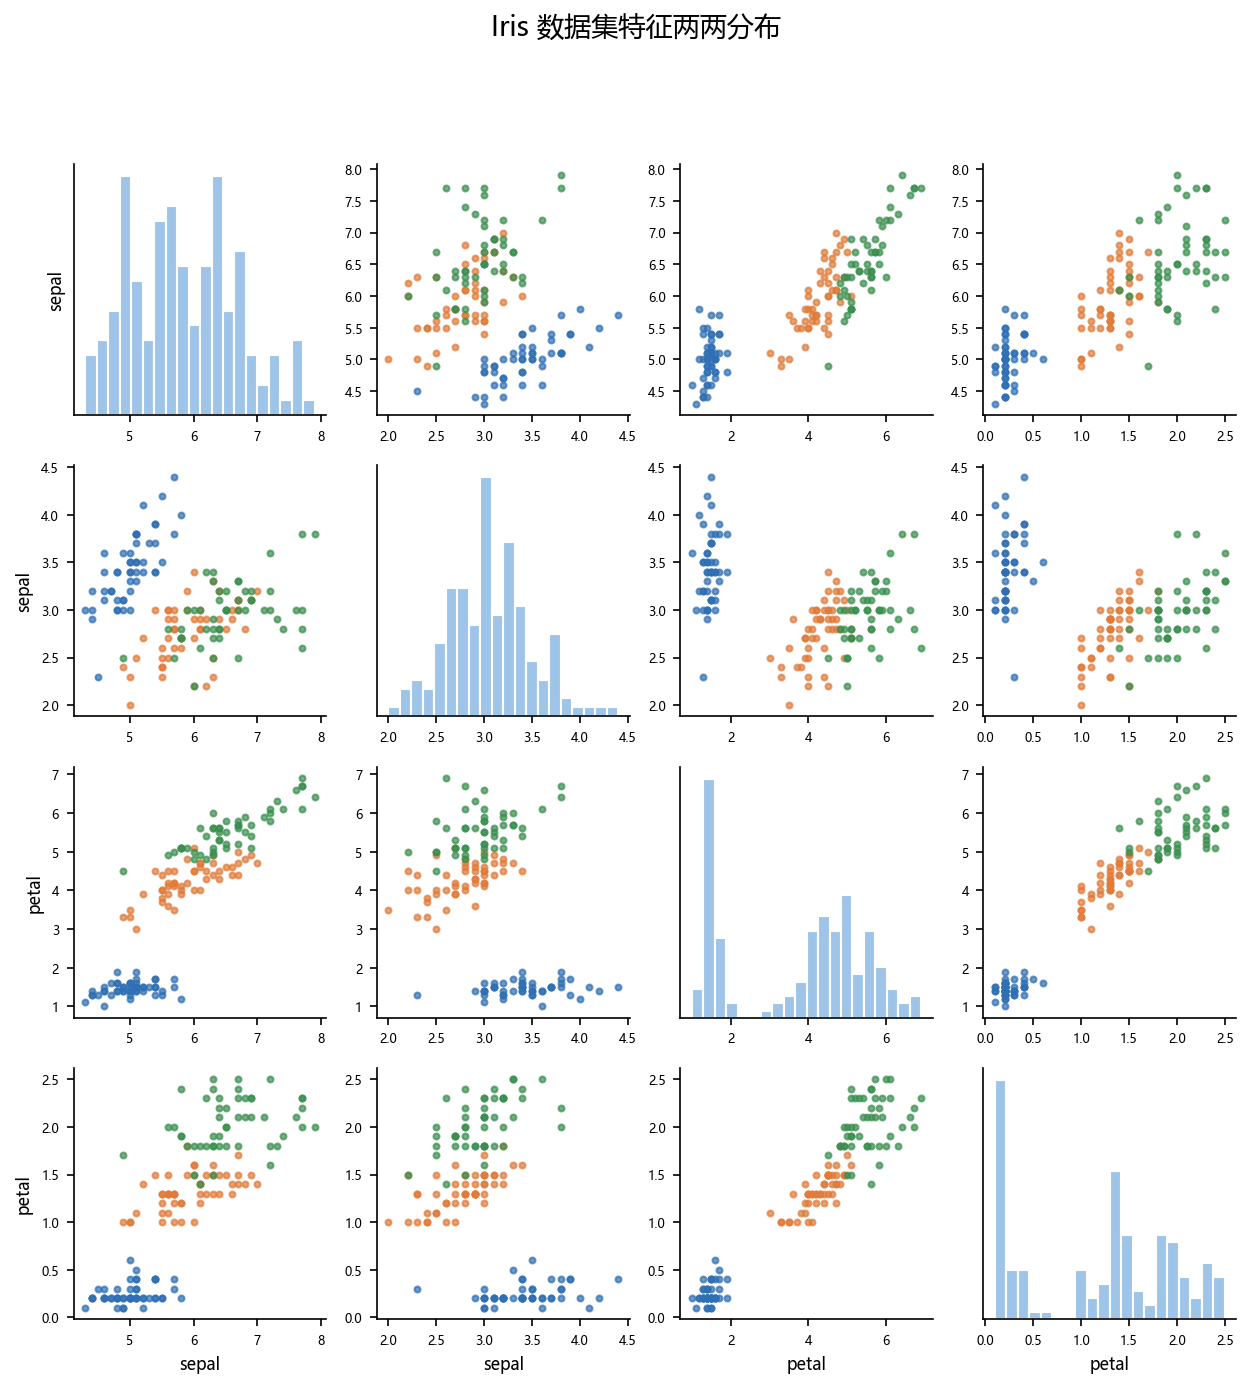
\includegraphics[keepaspectratio,alt={Iris 特征两两分布}]{figures/08-sklearn/iris_pairplot.png}}
\caption{Iris 特征两两分布}
\end{figure}

\paragraph{1.1
加载数据并切分}\label{ux52a0ux8f7dux6570ux636eux5e76ux5207ux5206}

\begin{Shaded}
\begin{Highlighting}[]
\ImportTok{import}\NormalTok{ numpy }\ImportTok{as}\NormalTok{ np}
\ImportTok{from}\NormalTok{ sklearn.datasets }\ImportTok{import}\NormalTok{ load\_iris}
\ImportTok{from}\NormalTok{ sklearn.model\_selection }\ImportTok{import}\NormalTok{ train\_test\_split}

\NormalTok{iris }\OperatorTok{=}\NormalTok{ load\_iris()}
\NormalTok{X, y }\OperatorTok{=}\NormalTok{ iris.data, iris.target}
\BuiltInTok{print}\NormalTok{(}\StringTok{"特征名:"}\NormalTok{, iris.feature\_names)}
\BuiltInTok{print}\NormalTok{(}\StringTok{"标签名:"}\NormalTok{, iris.target\_names)}
\BuiltInTok{print}\NormalTok{(}\StringTok{"数据形状:"}\NormalTok{, X.shape)}

\NormalTok{Xtr, Xte, ytr, yte }\OperatorTok{=}\NormalTok{ train\_test\_split(X, y, test\_size}\OperatorTok{=}\FloatTok{0.3}\NormalTok{, random\_state}\OperatorTok{=}\DecValTok{42}\NormalTok{, stratify}\OperatorTok{=}\NormalTok{y)}
\BuiltInTok{print}\NormalTok{(}\StringTok{"train/test:"}\NormalTok{, Xtr.shape, Xte.shape)}
\end{Highlighting}
\end{Shaded}

\begin{Shaded}
\begin{Highlighting}[]
\NormalTok{特征名: [\textquotesingle{}sepal length (cm)\textquotesingle{}, \textquotesingle{}sepal width (cm)\textquotesingle{}, \textquotesingle{}petal length (cm)\textquotesingle{}, \textquotesingle{}petal width (cm)\textquotesingle{}]}
\NormalTok{标签名: [\textquotesingle{}setosa\textquotesingle{} \textquotesingle{}versicolor\textquotesingle{} \textquotesingle{}virginica\textquotesingle{}]}
\NormalTok{数据形状: (150, 4)}
\NormalTok{train/test: (105, 4) (45, 4)}
\end{Highlighting}
\end{Shaded}

\paragraph{1.2
训练多个分类器并比较}\label{ux8badux7ec3ux591aux4e2aux5206ux7c7bux5668ux5e76ux6bd4ux8f83}

\begin{Shaded}
\begin{Highlighting}[]
\ImportTok{from}\NormalTok{ sklearn.neighbors }\ImportTok{import}\NormalTok{ KNeighborsClassifier}
\ImportTok{from}\NormalTok{ sklearn.linear\_model }\ImportTok{import}\NormalTok{ LogisticRegression}
\ImportTok{from}\NormalTok{ sklearn.tree }\ImportTok{import}\NormalTok{ DecisionTreeClassifier}
\ImportTok{from}\NormalTok{ sklearn.ensemble }\ImportTok{import}\NormalTok{ RandomForestClassifier}
\ImportTok{from}\NormalTok{ sklearn.metrics }\ImportTok{import}\NormalTok{ accuracy\_score}

\NormalTok{models }\OperatorTok{=}\NormalTok{ \{}
    \StringTok{"KNN(k=5)"}\NormalTok{: KNeighborsClassifier(n\_neighbors}\OperatorTok{=}\DecValTok{5}\NormalTok{),}
    \StringTok{"LogisticRegression"}\NormalTok{: LogisticRegression(max\_iter}\OperatorTok{=}\DecValTok{1000}\NormalTok{),}
    \StringTok{"DecisionTree"}\NormalTok{: DecisionTreeClassifier(random\_state}\OperatorTok{=}\DecValTok{42}\NormalTok{),}
    \StringTok{"RandomForest(100)"}\NormalTok{: RandomForestClassifier(n\_estimators}\OperatorTok{=}\DecValTok{100}\NormalTok{, random\_state}\OperatorTok{=}\DecValTok{42}\NormalTok{),}
\NormalTok{\}}
\ControlFlowTok{for}\NormalTok{ name, m }\KeywordTok{in}\NormalTok{ models.items():}
\NormalTok{    m.fit(Xtr, ytr)}
    \BuiltInTok{print}\NormalTok{(}\SpecialStringTok{f"}\SpecialCharTok{\{}\NormalTok{name}\SpecialCharTok{:22s\}}\SpecialStringTok{ acc = }\SpecialCharTok{\{}\NormalTok{accuracy\_score(yte, m.predict(Xte))}\SpecialCharTok{:.4f\}}\SpecialStringTok{"}\NormalTok{)}
\end{Highlighting}
\end{Shaded}

\begin{Shaded}
\begin{Highlighting}[]
\NormalTok{KNN(k=5)              acc = 0.9778}
\NormalTok{LogisticRegression    acc = 0.9333}
\NormalTok{DecisionTree          acc = 0.9333}
\NormalTok{RandomForest(100)     acc = 0.8889}
\end{Highlighting}
\end{Shaded}

\begin{quote}
不同模型在同一数据上表现不同，没有对任何数据集都最优的``万能模型''。随机森林在这份固定切分上反而略低，说明小样本下模型选择要看交叉验证与多次随机切分，而非一次
test 结果。
\end{quote}

\paragraph{1.3
混淆矩阵与分类报告}\label{ux6df7ux6dc6ux77e9ux9635ux4e0eux5206ux7c7bux62a5ux544a}

\begin{Shaded}
\begin{Highlighting}[]
\ImportTok{from}\NormalTok{ sklearn.metrics }\ImportTok{import}\NormalTok{ confusion\_matrix, classification\_report}

\NormalTok{rf }\OperatorTok{=}\NormalTok{ models[}\StringTok{"RandomForest(100)"}\NormalTok{]}
\BuiltInTok{print}\NormalTok{(confusion\_matrix(yte, rf.predict(Xte)))}
\BuiltInTok{print}\NormalTok{(classification\_report(yte, rf.predict(Xte), target\_names}\OperatorTok{=}\NormalTok{iris.target\_names))}
\end{Highlighting}
\end{Shaded}

\begin{Shaded}
\begin{Highlighting}[]
\NormalTok{[[15  0  0]}
\NormalTok{ [ 0 14  1]}
\NormalTok{ [ 0  4 11]]}
\NormalTok{              precision    recall  f1{-}score   support}

\NormalTok{      setosa       1.00      1.00      1.00        15}
\NormalTok{  versicolor       0.78      0.93      0.85        15}
\NormalTok{   virginica       0.92      0.73      0.81        15}

\NormalTok{    accuracy                           0.89        45}
\NormalTok{   macro avg       0.90      0.89      0.89        45}
\NormalTok{weighted avg       0.90      0.89      0.89        45}
\end{Highlighting}
\end{Shaded}

\begin{quote}
混淆矩阵第 i 行第 j 列表示``真实为 i、被判为
j''。\texttt{classification\_report} 给出每类的
precision、recall、f1。对不平衡数据，准确率会误导，要看 f1/recall。
\end{quote}

\paragraph{1.4 决策树可视化}\label{ux51b3ux7b56ux6811ux53efux89c6ux5316}

\begin{Shaded}
\begin{Highlighting}[]
\ImportTok{import}\NormalTok{ matplotlib.pyplot }\ImportTok{as}\NormalTok{ plt}
\NormalTok{plt.rcParams[}\StringTok{"font.sans{-}serif"}\NormalTok{] }\OperatorTok{=}\NormalTok{ [}\StringTok{"Microsoft YaHei"}\NormalTok{, }\StringTok{"SimHei"}\NormalTok{, }\StringTok{"DejaVu Sans"}\NormalTok{]}
\NormalTok{plt.rcParams[}\StringTok{"axes.unicode\_minus"}\NormalTok{] }\OperatorTok{=} \VariableTok{False}
\ImportTok{from}\NormalTok{ sklearn.tree }\ImportTok{import}\NormalTok{ plot\_tree}

\NormalTok{dt }\OperatorTok{=}\NormalTok{ DecisionTreeClassifier(max\_depth}\OperatorTok{=}\DecValTok{3}\NormalTok{, random\_state}\OperatorTok{=}\DecValTok{42}\NormalTok{).fit(Xtr, ytr)}
\NormalTok{fig, ax }\OperatorTok{=}\NormalTok{ plt.subplots(figsize}\OperatorTok{=}\NormalTok{(}\DecValTok{13}\NormalTok{, }\DecValTok{7}\NormalTok{))}
\NormalTok{plot\_tree(dt, feature\_names}\OperatorTok{=}\NormalTok{iris.feature\_names,}
\NormalTok{          class\_names}\OperatorTok{=}\BuiltInTok{list}\NormalTok{(iris.target\_names), filled}\OperatorTok{=}\VariableTok{True}\NormalTok{, rounded}\OperatorTok{=}\VariableTok{True}\NormalTok{, ax}\OperatorTok{=}\NormalTok{ax, fontsize}\OperatorTok{=}\DecValTok{8}\NormalTok{)}
\NormalTok{plt.title(}\StringTok{"Iris 决策树（max\_depth=3）"}\NormalTok{)}
\end{Highlighting}
\end{Shaded}

\begin{figure}
\centering
\pandocbounded{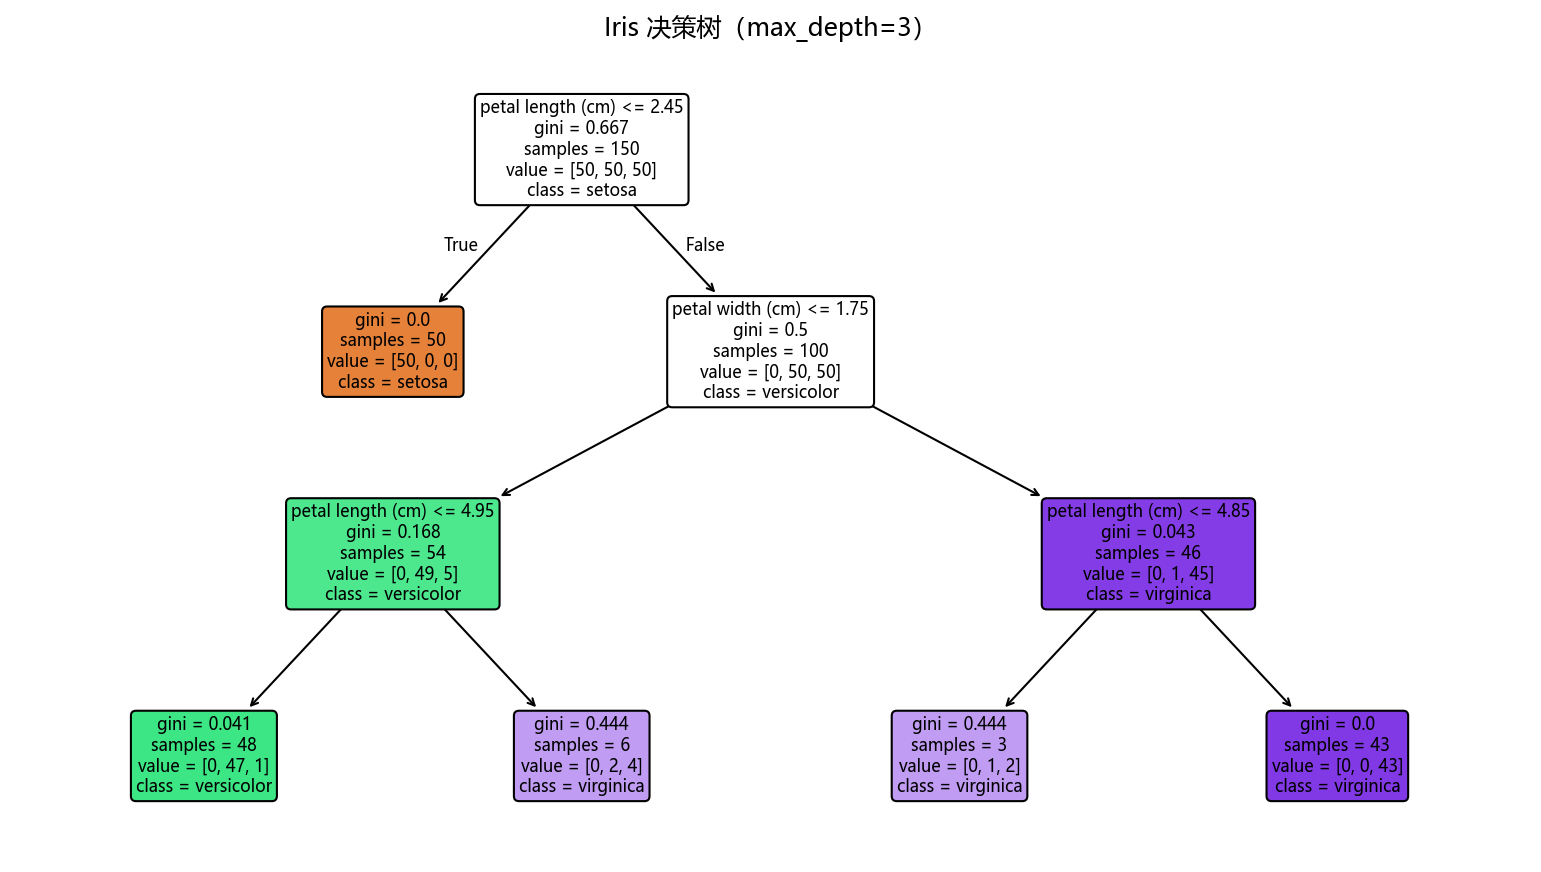
\includegraphics[keepaspectratio,alt={Iris 决策树}]{figures/08-sklearn/decision_tree_iris.png}}
\caption{Iris 决策树}
\end{figure}

\subsubsection{2. 二分类与
ROC-AUC：乳腺癌}\label{ux4e8cux5206ux7c7bux4e0e-roc-aucux4e73ux817aux764c}

乳腺癌数据集是二分类（良性/恶性）。逻辑回归对量纲敏感，因此用
\texttt{Pipeline} 先标准化再训练。

\begin{Shaded}
\begin{Highlighting}[]
\ImportTok{from}\NormalTok{ sklearn.datasets }\ImportTok{import}\NormalTok{ load\_breast\_cancer}
\ImportTok{from}\NormalTok{ sklearn.model\_selection }\ImportTok{import}\NormalTok{ train\_test\_split}
\ImportTok{from}\NormalTok{ sklearn.pipeline }\ImportTok{import}\NormalTok{ Pipeline}
\ImportTok{from}\NormalTok{ sklearn.preprocessing }\ImportTok{import}\NormalTok{ StandardScaler}
\ImportTok{from}\NormalTok{ sklearn.linear\_model }\ImportTok{import}\NormalTok{ LogisticRegression}
\ImportTok{from}\NormalTok{ sklearn.metrics }\ImportTok{import}\NormalTok{ accuracy\_score, roc\_auc\_score}

\NormalTok{bc }\OperatorTok{=}\NormalTok{ load\_breast\_cancer()}\OperatorTok{;}\NormalTok{ Xb, yb }\OperatorTok{=}\NormalTok{ bc.data, bc.target}
\NormalTok{Xtr, Xte, ytr, yte }\OperatorTok{=}\NormalTok{ train\_test\_split(Xb, yb, test\_size}\OperatorTok{=}\FloatTok{0.3}\NormalTok{, random\_state}\OperatorTok{=}\DecValTok{42}\NormalTok{, stratify}\OperatorTok{=}\NormalTok{yb)}

\NormalTok{pipe }\OperatorTok{=}\NormalTok{ Pipeline([(}\StringTok{"sc"}\NormalTok{, StandardScaler()), (}\StringTok{"clf"}\NormalTok{, LogisticRegression(max\_iter}\OperatorTok{=}\DecValTok{1000}\NormalTok{))])}
\NormalTok{pipe.fit(Xtr, ytr)}
\NormalTok{prob }\OperatorTok{=}\NormalTok{ pipe.predict\_proba(Xte)[:, }\DecValTok{1}\NormalTok{]}
\BuiltInTok{print}\NormalTok{(}\StringTok{"ROC{-}AUC:"}\NormalTok{, }\BuiltInTok{round}\NormalTok{(roc\_auc\_score(yte, prob), }\DecValTok{4}\NormalTok{))}
\BuiltInTok{print}\NormalTok{(}\StringTok{"准确率:"}\NormalTok{, }\BuiltInTok{round}\NormalTok{(accuracy\_score(yte, pipe.predict(Xte)), }\DecValTok{4}\NormalTok{))}
\end{Highlighting}
\end{Shaded}

\begin{Shaded}
\begin{Highlighting}[]
\NormalTok{ROC{-}AUC: 0.9981}
\NormalTok{准确率: 0.9883}
\end{Highlighting}
\end{Shaded}

\begin{quote}
\texttt{predict\_proba}
返回每个样本属于正类的概率；\texttt{roc\_auc\_score}
评估``排序能力''，比单纯准确率更能反映二分类模型质量。
\end{quote}

\textbf{缩放为什么关键}：SVC/KNN 对量纲很敏感。下图给出乳腺癌 5
折交叉验证，未标准化 vs 标准化的对比：

\begin{figure}
\centering
\pandocbounded{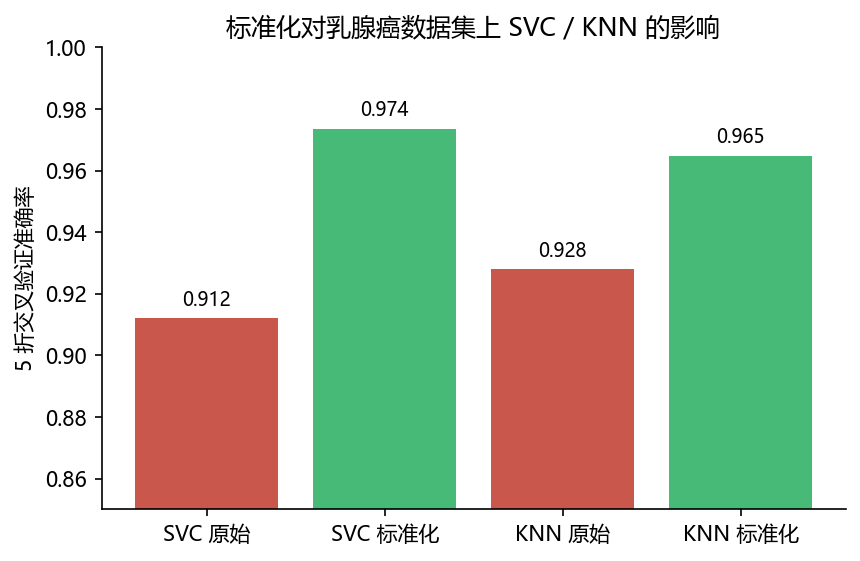
\includegraphics[keepaspectratio,alt={缩放影响}]{figures/08-sklearn/scaling_effect.png}}
\caption{缩放影响}
\end{figure}

\subsubsection{3. 回归：Diabetes
糖尿病}\label{ux56deux5f52diabetes-ux7cd6ux5c3fux75c5}

波士顿房价数据集（\texttt{load\_boston}）已在 sklearn 1.2
被移除，故本节改用内置的 \texttt{load\_diabetes}（442 个样本、10
个标准化后的特征）。

\begin{Shaded}
\begin{Highlighting}[]
\ImportTok{from}\NormalTok{ sklearn.datasets }\ImportTok{import}\NormalTok{ load\_diabetes}
\ImportTok{from}\NormalTok{ sklearn.model\_selection }\ImportTok{import}\NormalTok{ train\_test\_split}
\ImportTok{from}\NormalTok{ sklearn.linear\_model }\ImportTok{import}\NormalTok{ LinearRegression, Ridge, Lasso}
\ImportTok{from}\NormalTok{ sklearn.metrics }\ImportTok{import}\NormalTok{ mean\_squared\_error, mean\_absolute\_error, r2\_score}
\ImportTok{import}\NormalTok{ numpy }\ImportTok{as}\NormalTok{ np}

\NormalTok{d }\OperatorTok{=}\NormalTok{ load\_diabetes()}\OperatorTok{;}\NormalTok{ Xd, yd }\OperatorTok{=}\NormalTok{ d.data, d.target}
\NormalTok{Xtr, Xte, ytr, yte }\OperatorTok{=}\NormalTok{ train\_test\_split(Xd, yd, test\_size}\OperatorTok{=}\FloatTok{0.2}\NormalTok{, random\_state}\OperatorTok{=}\DecValTok{42}\NormalTok{)}

\ControlFlowTok{for}\NormalTok{ name, m }\KeywordTok{in}\NormalTok{ [(}\StringTok{"LinearRegression"}\NormalTok{, LinearRegression()),}
\NormalTok{                (}\StringTok{"Ridge(alpha=1)"}\NormalTok{, Ridge(alpha}\OperatorTok{=}\FloatTok{1.0}\NormalTok{)),}
\NormalTok{                (}\StringTok{"Lasso(alpha=0.1)"}\NormalTok{, Lasso(alpha}\OperatorTok{=}\FloatTok{0.1}\NormalTok{, max\_iter}\OperatorTok{=}\DecValTok{5000}\NormalTok{))]:}
\NormalTok{    m.fit(Xtr, ytr)}
\NormalTok{    yp }\OperatorTok{=}\NormalTok{ m.predict(Xte)}
    \BuiltInTok{print}\NormalTok{(}\SpecialStringTok{f"}\SpecialCharTok{\{}\NormalTok{name}\SpecialCharTok{:20s\}}\SpecialStringTok{ MSE=}\SpecialCharTok{\{}\NormalTok{mean\_squared\_error(yte, yp)}\SpecialCharTok{:.2f\}}\SpecialStringTok{  "}
          \SpecialStringTok{f"MAE=}\SpecialCharTok{\{}\NormalTok{mean\_absolute\_error(yte, yp)}\SpecialCharTok{:.2f\}}\SpecialStringTok{  R2=}\SpecialCharTok{\{}\NormalTok{r2\_score(yte, yp)}\SpecialCharTok{:.4f\}}\SpecialStringTok{"}\NormalTok{)}

\NormalTok{las }\OperatorTok{=}\NormalTok{ Lasso(alpha}\OperatorTok{=}\FloatTok{0.1}\NormalTok{, max\_iter}\OperatorTok{=}\DecValTok{5000}\NormalTok{).fit(Xtr, ytr)}
\BuiltInTok{print}\NormalTok{(}\StringTok{"Lasso 非零系数个数:"}\NormalTok{, np.count\_nonzero(las.coef\_))}
\BuiltInTok{print}\NormalTok{(}\StringTok{"特征名:"}\NormalTok{, d.feature\_names)}
\end{Highlighting}
\end{Shaded}

\begin{Shaded}
\begin{Highlighting}[]
\NormalTok{LinearRegression    MSE=2900.19  MAE=42.79  R2=0.4526}
\NormalTok{Ridge(alpha=1)      MSE=3077.42  MAE=46.14  R2=0.4192}
\NormalTok{Lasso(alpha=0.1)    MSE=2798.19  MAE=42.85  R2=0.4719}
\NormalTok{Lasso 非零系数个数: 7}
\NormalTok{特征名: [\textquotesingle{}age\textquotesingle{}, \textquotesingle{}sex\textquotesingle{}, \textquotesingle{}bmi\textquotesingle{}, \textquotesingle{}bp\textquotesingle{}, \textquotesingle{}s1\textquotesingle{}, \textquotesingle{}s2\textquotesingle{}, \textquotesingle{}s3\textquotesingle{}, \textquotesingle{}s4\textquotesingle{}, \textquotesingle{}s5\textquotesingle{}, \textquotesingle{}s6\textquotesingle{}]}
\end{Highlighting}
\end{Shaded}

\begin{quote}
回归指标速记：\texttt{MSE}/\texttt{MAE} 越小越好；\texttt{R2} 越接近 1
越好。这里 Lasso 用 L1 正则把部分系数压到 0，既得到不错 R²
又做了特征选择。
\end{quote}

\subsection{常见误区}\label{ux5e38ux89c1ux8befux533a-22}

\begin{enumerate}
\def\labelenumi{\arabic{enumi}.}
\tightlist
\item
  用 \texttt{r2\_score(y\_pred,\ y\_test)} 参数顺序写反 → 应为
  \texttt{r2\_score(y\_true,\ y\_pred)}；对分类问题更不该用 R²。
\item
  在 sklearn 里已经移除 \texttt{load\_boston}，再用会
  \texttt{ImportError}。
\item
  直接拿未缩放数据喂
  \texttt{SVC}/\texttt{KNN}/\texttt{LogisticRegression}，会导致收敛慢或精度差。
\item
  把 \texttt{predict\_proba} 的第一列当作正类概率 → 正类是第 1
  列（标签为 1 的类）。
\item
  在同一个数据集上反复``调参、看测试集''，相当于把测试集当训练信息用。
\end{enumerate}

\subsection{思考题}\label{ux601dux8003ux9898-22}

\begin{enumerate}
\def\labelenumi{\arabic{enumi}.}
\tightlist
\item
  为什么 KNN 对缩放特别敏感？树模型为什么相对不敏感？
\item
  \texttt{accuracy\_score} 与 \texttt{roc\_auc\_score}
  分别衡量什么？在类别不平衡时哪个更可靠？
\item
  一次 test 集准确率高，能说明模型泛化好吗？为什么还要交叉验证？
\end{enumerate}

\subsection{动手练习}\label{ux52a8ux624bux7ec3ux4e60-6}

\begin{enumerate}
\def\labelenumi{\arabic{enumi}.}
\tightlist
\item
  在 Iris 上把 \texttt{RandomForestClassifier(n\_estimators=100)} 与
  \texttt{KNeighborsClassifier} 做 5 折交叉验证比较。
\item
  用 \texttt{SVC} 分别在不缩放/缩放情况下做乳腺癌 5 折，记录结果（可对照
  \texttt{scaling\_effect.png}）。
\item
  在 Diabetes 上试 \texttt{Ridge(alpha)} 与 \texttt{Lasso(alpha)} 的不同
  \texttt{alpha} 值，画出``alpha-R²''曲线。
\end{enumerate}

\subsection{延伸阅读}\label{ux5ef6ux4f38ux9605ux8bfb-35}

\begin{itemize}
\tightlist
\item
  sklearn
  分类指标：https://scikit-learn.org/stable/modules/model\_evaluation.html\#classification-metrics
\item
  sklearn
  回归指标：https://scikit-learn.org/stable/modules/model\_evaluation.html\#regression-metrics
\item
  sklearn
  用户指南``选择正确的评估器''：https://scikit-learn.org/stable/modules/preprocessing.html
\end{itemize}

\section{03
无监督学习的案例}\label{ux65e0ux76d1ux7763ux5b66ux4e60ux7684ux6848ux4f8b}

\begin{quote}
本节讲``没有标签''的任务：\textbf{聚类}（KMeans、DBSCAN）与\textbf{降维}（PCA、LDA）。所有代码在
sklearn 1.6.1 下验证。
\end{quote}

\subsection{本节目标}\label{ux672cux8282ux76eeux6807-23}

\begin{enumerate}
\def\labelenumi{\arabic{enumi}.}
\tightlist
\item
  用 \texttt{KMeans} 对 \texttt{make\_blobs} 聚类，读出
  \texttt{inertia\_}、\texttt{cluster\_centers\_}、\texttt{silhouette\_score}。
\item
  用 \texttt{DBSCAN} 对 \texttt{make\_moons} 聚类，识别噪声（标签
  -1），并算 \texttt{adjusted\_rand\_score}。
\item
  用 \texttt{PCA} 降维并读出 \texttt{explained\_variance\_ratio\_}。
\item
  用 \texttt{LDA} 做有监督降维，理解它与 PCA 的差别。
\end{enumerate}

\subsection{先修}\label{ux5148ux4fee-23}

\begin{itemize}
\tightlist
\item
  01 节特征缩放、02 节分类/回归基础。
\item
  了解``距离''\,``方差''\,``协方差''等概念。
\end{itemize}

\subsection{官方文档 /
参考入口}\label{ux5b98ux65b9ux6587ux6863-ux53c2ux8003ux5165ux53e3-9}

\begin{itemize}
\tightlist
\item
  sklearn 聚类：https://scikit-learn.org/stable/modules/clustering.html
\item
  sklearn
  降维：https://scikit-learn.org/stable/modules/decomposition.html
\item
  sklearn
  聚类评估：https://scikit-learn.org/stable/modules/clustering.html\#clustering-performance-evaluation
\end{itemize}

\subsection{正文}\label{ux6b63ux6587-2}

\subsubsection{1. 聚类：KMeans}\label{ux805aux7c7bkmeans}

KMeans 把数据分成 K 个簇，使``簇内平方和''最小。它需要预先指定 K。

\begin{Shaded}
\begin{Highlighting}[]
\ImportTok{import}\NormalTok{ numpy }\ImportTok{as}\NormalTok{ np}
\ImportTok{from}\NormalTok{ sklearn.cluster }\ImportTok{import}\NormalTok{ KMeans}
\ImportTok{from}\NormalTok{ sklearn.datasets }\ImportTok{import}\NormalTok{ make\_blobs}
\ImportTok{from}\NormalTok{ sklearn.metrics }\ImportTok{import}\NormalTok{ silhouette\_score}

\NormalTok{X, \_ }\OperatorTok{=}\NormalTok{ make\_blobs(n\_samples}\OperatorTok{=}\DecValTok{300}\NormalTok{, centers}\OperatorTok{=}\DecValTok{4}\NormalTok{, cluster\_std}\OperatorTok{=}\FloatTok{0.60}\NormalTok{, random\_state}\OperatorTok{=}\DecValTok{0}\NormalTok{)}
\NormalTok{km }\OperatorTok{=}\NormalTok{ KMeans(n\_clusters}\OperatorTok{=}\DecValTok{4}\NormalTok{, random\_state}\OperatorTok{=}\DecValTok{0}\NormalTok{).fit(X)}
\NormalTok{labels }\OperatorTok{=}\NormalTok{ km.labels\_}
\BuiltInTok{print}\NormalTok{(}\StringTok{"inertia:"}\NormalTok{, }\BuiltInTok{round}\NormalTok{(km.inertia\_, }\DecValTok{4}\NormalTok{))}
\BuiltInTok{print}\NormalTok{(}\StringTok{"聚类中心形状:"}\NormalTok{, km.cluster\_centers\_.shape)}
\BuiltInTok{print}\NormalTok{(}\StringTok{"轮廓系数:"}\NormalTok{, }\BuiltInTok{round}\NormalTok{(silhouette\_score(X, labels), }\DecValTok{4}\NormalTok{))}
\end{Highlighting}
\end{Shaded}

\begin{Shaded}
\begin{Highlighting}[]
\NormalTok{inertia: 212.006}
\NormalTok{聚类中心形状: (4, 2)}
\NormalTok{轮廓系数: 0.682}
\end{Highlighting}
\end{Shaded}

\begin{quote}
\texttt{inertia\_} 是簇内平方和，越小越好；\texttt{silhouette\_score} 在
{[}-1,1{]} 之间，越接近 1 表示簇内紧凑、簇间分离越好。
\end{quote}

\subsubsection{2. 聚类：DBSCAN}\label{ux805aux7c7bdbscan}

DBSCAN 按密度自动发现簇，能处理任意形状，并能把不属于任何簇的点标为
\textbf{-1（噪声）}。

\begin{Shaded}
\begin{Highlighting}[]
\ImportTok{from}\NormalTok{ sklearn.cluster }\ImportTok{import}\NormalTok{ DBSCAN}
\ImportTok{from}\NormalTok{ sklearn.datasets }\ImportTok{import}\NormalTok{ make\_moons}
\ImportTok{from}\NormalTok{ sklearn.metrics }\ImportTok{import}\NormalTok{ adjusted\_rand\_score}

\NormalTok{Xm, ym }\OperatorTok{=}\NormalTok{ make\_moons(n\_samples}\OperatorTok{=}\DecValTok{300}\NormalTok{, noise}\OperatorTok{=}\FloatTok{0.1}\NormalTok{, random\_state}\OperatorTok{=}\DecValTok{42}\NormalTok{)}
\NormalTok{db }\OperatorTok{=}\NormalTok{ DBSCAN(eps}\OperatorTok{=}\FloatTok{0.2}\NormalTok{, min\_samples}\OperatorTok{=}\DecValTok{5}\NormalTok{).fit(Xm)}
\NormalTok{labels }\OperatorTok{=}\NormalTok{ db.labels\_}
\BuiltInTok{print}\NormalTok{(}\StringTok{"簇数:"}\NormalTok{, }\BuiltInTok{len}\NormalTok{(}\BuiltInTok{set}\NormalTok{(labels)) }\OperatorTok{{-}}\NormalTok{ (}\DecValTok{1} \ControlFlowTok{if} \OperatorTok{{-}}\DecValTok{1} \KeywordTok{in}\NormalTok{ labels }\ControlFlowTok{else} \DecValTok{0}\NormalTok{))}
\BuiltInTok{print}\NormalTok{(}\StringTok{"噪声比例:"}\NormalTok{, }\BuiltInTok{round}\NormalTok{(np.mean(labels }\OperatorTok{==} \OperatorTok{{-}}\DecValTok{1}\NormalTok{), }\DecValTok{4}\NormalTok{))}
\BuiltInTok{print}\NormalTok{(}\StringTok{"簇大小:"}\NormalTok{, np.bincount(labels))}
\BuiltInTok{print}\NormalTok{(}\StringTok{"与真实标签 ARI:"}\NormalTok{, }\BuiltInTok{round}\NormalTok{(adjusted\_rand\_score(ym, labels), }\DecValTok{4}\NormalTok{))}
\end{Highlighting}
\end{Shaded}

\begin{Shaded}
\begin{Highlighting}[]
\NormalTok{簇数: 2}
\NormalTok{噪声比例: 0.0}
\NormalTok{簇大小: [150 150]}
\NormalTok{与真实标签 ARI: 1.0}
\end{Highlighting}
\end{Shaded}

\begin{quote}
\texttt{adjusted\_rand\_score}（ARI）在 {[}0,1{]}（随机约 0、完全一致为
1）。这里 DBSCAN 完美分出两个月牙形簇，ARI=1.0。
\end{quote}

\textbf{KMeans 与 DBSCAN 的对比}：KMeans
假设凸形、球形簇，对``弯月''类数据效果差；DBSCAN
依据密度，可发现任意形状并识别噪声。

\begin{figure}
\centering
\pandocbounded{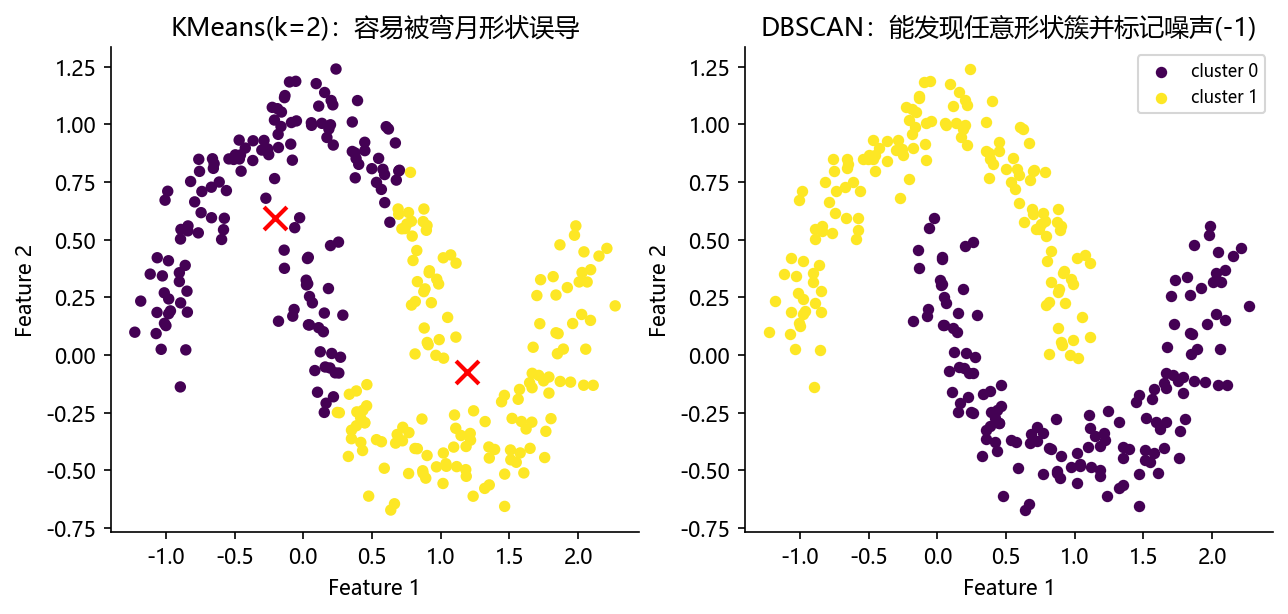
\includegraphics[keepaspectratio,alt={KMeans vs DBSCAN}]{figures/08-sklearn/dbscan_kmeans_moons.png}}
\caption{KMeans vs DBSCAN}
\end{figure}

\subsubsection{3.
降维：PCA（无监督）}\label{ux964dux7ef4pcaux65e0ux76d1ux7763}

PCA 找``方差最大的方向''，把高维映射到低维，且不需要标签。

\begin{Shaded}
\begin{Highlighting}[]
\ImportTok{from}\NormalTok{ sklearn.datasets }\ImportTok{import}\NormalTok{ load\_iris}
\ImportTok{from}\NormalTok{ sklearn.decomposition }\ImportTok{import}\NormalTok{ PCA}

\NormalTok{iris }\OperatorTok{=}\NormalTok{ load\_iris()}\OperatorTok{;}\NormalTok{ X, y }\OperatorTok{=}\NormalTok{ iris.data, iris.target}
\NormalTok{pca }\OperatorTok{=}\NormalTok{ PCA(n\_components}\OperatorTok{=}\DecValTok{2}\NormalTok{)}
\NormalTok{Xp }\OperatorTok{=}\NormalTok{ pca.fit\_transform(X)}
\BuiltInTok{print}\NormalTok{(}\StringTok{"各主成分解释方差比:"}\NormalTok{, np.}\BuiltInTok{round}\NormalTok{(pca.explained\_variance\_ratio\_, }\DecValTok{4}\NormalTok{))}
\BuiltInTok{print}\NormalTok{(}\StringTok{"累计解释方差:"}\NormalTok{, np.}\BuiltInTok{round}\NormalTok{(np.cumsum(pca.explained\_variance\_ratio\_), }\DecValTok{4}\NormalTok{))}
\end{Highlighting}
\end{Shaded}

\begin{Shaded}
\begin{Highlighting}[]
\NormalTok{各主成分解释方差比: [0.9246 0.0531]}
\NormalTok{累计解释方差: [0.9246 0.9777]}
\end{Highlighting}
\end{Shaded}

\begin{quote}
前 2 个主成分已保留约 97.77\% 方差，说明 Iris 降到 2
维几乎不丢信息，适合可视化。
\end{quote}

\subsubsection{4.
降维：LDA（有监督）}\label{ux964dux7ef4ldaux6709ux76d1ux7763}

LDA
在已知类别的情况下，找``类间方差最大、类内方差最小''的投影方向。因此需要同时给出
\texttt{X} 与 \texttt{y}。

\begin{Shaded}
\begin{Highlighting}[]
\ImportTok{from}\NormalTok{ sklearn.discriminant\_analysis }\ImportTok{import}\NormalTok{ LinearDiscriminantAnalysis }\ImportTok{as}\NormalTok{ LDA}

\NormalTok{lda }\OperatorTok{=}\NormalTok{ LDA(n\_components}\OperatorTok{=}\DecValTok{2}\NormalTok{)}
\NormalTok{Xl }\OperatorTok{=}\NormalTok{ lda.fit\_transform(X, y)}
\BuiltInTok{print}\NormalTok{(}\StringTok{"LDA 各成分解释方差比:"}\NormalTok{, np.}\BuiltInTok{round}\NormalTok{(lda.explained\_variance\_ratio\_, }\DecValTok{4}\NormalTok{))}
\end{Highlighting}
\end{Shaded}

\begin{Shaded}
\begin{Highlighting}[]
\NormalTok{LDA 各成分解释方差比: [0.9912 0.0088]}
\end{Highlighting}
\end{Shaded}

\begin{quote}
对比：PCA 完全不看类别，LDA
用类别信息，因而投影对分类更有帮助。两者都适用于 Iris 降到 2
维，但语义不同。
\end{quote}

\subsection{常见误区}\label{ux5e38ux89c1ux8befux533a-23}

\begin{enumerate}
\def\labelenumi{\arabic{enumi}.}
\tightlist
\item
  KMeans 必须预设 \texttt{n\_clusters}，且对初始中心敏感（用
  \texttt{random\_state} 固定，或用 \texttt{k-means++}）。
\item
  以为``降维能提升所有模型精度''------降维会丢失信息，有时反而更差。
\item
  把 PCA 与 LDA 混为一谈（前者无监督、后者有监督）。
\item
  对 \texttt{make\_moons} 用 KMeans 期望得到月牙形簇------通常失败。
\item
  \texttt{DBSCAN} 的 \texttt{eps}、\texttt{min\_samples}
  必须按数据量纲调，不能``一个参数跑天下''。
\end{enumerate}

\subsection{思考题}\label{ux601dux8003ux9898-23}

\begin{enumerate}
\def\labelenumi{\arabic{enumi}.}
\tightlist
\item
  为什么 KMeans 需要先缩放？PCA 呢？
\item
  DBSCAN 的 \texttt{eps} 太小/太大会分别出现什么现象？
\item
  用什么指标判断``该保留多少个主成分''？（累计解释方差、碎石图等）
\item
  ARI 与 \texttt{silhouette\_score} 的适用场景有何不同？
\end{enumerate}

\subsection{动手练习}\label{ux52a8ux624bux7ec3ux4e60-7}

\begin{enumerate}
\def\labelenumi{\arabic{enumi}.}
\tightlist
\item
  对 \texttt{make\_blobs} 用 \texttt{KMeans(k=2..6)}
  画出``k-轮廓系数''曲线，找最佳 k。
\item
  调整 \texttt{DBSCAN} 的
  \texttt{eps}（0.1/0.2/0.5），观察簇数与噪声比例变化。
\item
  对 Wine 数据（13 维）用 PCA 降到 2 维并散点着色，给出累计解释方差。
\end{enumerate}

\subsection{延伸阅读}\label{ux5ef6ux4f38ux9605ux8bfb-36}

\begin{itemize}
\tightlist
\item
  sklearn
  聚类用户指南：https://scikit-learn.org/stable/modules/clustering.html
\item
  sklearn
  降维用户指南：https://scikit-learn.org/stable/modules/decomposition.html
\item
  sklearn
  聚类评估：https://scikit-learn.org/stable/modules/clustering.html\#clustering-performance-evaluation
\end{itemize}

\section{04 综合案例：Wine 数据端到端（预处理 → 分类 → 聚类 →
降维）}\label{ux7efcux5408ux6848ux4f8bwine-ux6570ux636eux7aefux5230ux7aefux9884ux5904ux7406-ux5206ux7c7b-ux805aux7c7b-ux964dux7ef4}

\begin{quote}
本章新增综合案例，把 01--03 的知识串成一条完整流水线：\textbf{特征缩放 →
分类 → 特征重要性 → 聚类 → 降维 → 可视化}。所有代码在 sklearn 1.6.1
下验证；配图由 \texttt{build/make\_chap8\_figures.py} 生成。
\end{quote}

\subsection{案例背景}\label{ux6848ux4f8bux80ccux666f-3}

Wine（红酒）数据集有 178 个样本、13
个数值特征（酒精、苹果酸、灰分、总酚、黄酮等），标签为 3
个品种（\texttt{class\_0/1/2}）。这是一个``数值特征多、量纲不同、类别有结构''的典型数据，非常适合练习本章全部知识。

\subsection{第 1
步：加载数据并观察}\label{ux7b2c-1-ux6b65ux52a0ux8f7dux6570ux636eux5e76ux89c2ux5bdf}

\begin{Shaded}
\begin{Highlighting}[]
\ImportTok{import}\NormalTok{ numpy }\ImportTok{as}\NormalTok{ np}
\ImportTok{from}\NormalTok{ sklearn.datasets }\ImportTok{import}\NormalTok{ load\_wine}

\NormalTok{wine }\OperatorTok{=}\NormalTok{ load\_wine()}
\NormalTok{X, y }\OperatorTok{=}\NormalTok{ wine.data, wine.target}
\BuiltInTok{print}\NormalTok{(}\StringTok{"特征名:"}\NormalTok{, wine.feature\_names)}
\BuiltInTok{print}\NormalTok{(}\StringTok{"数据形状:"}\NormalTok{, X.shape, }\StringTok{"类别:"}\NormalTok{, np.unique(y))}
\end{Highlighting}
\end{Shaded}

\begin{Shaded}
\begin{Highlighting}[]
\NormalTok{特征名: [\textquotesingle{}alcohol\textquotesingle{}, \textquotesingle{}malic\_acid\textquotesingle{}, \textquotesingle{}ash\textquotesingle{}, \textquotesingle{}alcalinity\_of\_ash\textquotesingle{}, \textquotesingle{}magnesium\textquotesingle{}, \textquotesingle{}total\_phenols\textquotesingle{}, \textquotesingle{}flavanoids\textquotesingle{}, \textquotesingle{}nonflavanoid\_phenols\textquotesingle{}, \textquotesingle{}proanthocyanins\textquotesingle{}, \textquotesingle{}color\_intensity\textquotesingle{}, \textquotesingle{}hue\textquotesingle{}, \textquotesingle{}od280/od315\_of\_diluted\_wines\textquotesingle{}, \textquotesingle{}proline\textquotesingle{}]}
\NormalTok{数据形状: (178, 13) 类别: [0 1 2]}
\end{Highlighting}
\end{Shaded}

\subsection{第 2 步：缩放 + 分类（用 Pipeline
防泄漏）}\label{ux7b2c-2-ux6b65ux7f29ux653e-ux5206ux7c7bux7528-pipeline-ux9632ux6cc4ux6f0f}

把``标准化''与``分类器''放进 \texttt{Pipeline}，这样
\texttt{cross\_val\_score}
每次都在训练折上拟合缩放器，绝不用测试折的信息。

\begin{Shaded}
\begin{Highlighting}[]
\ImportTok{from}\NormalTok{ sklearn.model\_selection }\ImportTok{import}\NormalTok{ train\_test\_split, cross\_val\_score}
\ImportTok{from}\NormalTok{ sklearn.preprocessing }\ImportTok{import}\NormalTok{ StandardScaler}
\ImportTok{from}\NormalTok{ sklearn.pipeline }\ImportTok{import}\NormalTok{ Pipeline}
\ImportTok{from}\NormalTok{ sklearn.linear\_model }\ImportTok{import}\NormalTok{ LogisticRegression}
\ImportTok{from}\NormalTok{ sklearn.ensemble }\ImportTok{import}\NormalTok{ RandomForestClassifier}
\ImportTok{from}\NormalTok{ sklearn.metrics }\ImportTok{import}\NormalTok{ accuracy\_score}

\NormalTok{Xtr, Xte, ytr, yte }\OperatorTok{=}\NormalTok{ train\_test\_split(X, y, test\_size}\OperatorTok{=}\FloatTok{0.3}\NormalTok{, random\_state}\OperatorTok{=}\DecValTok{42}\NormalTok{, stratify}\OperatorTok{=}\NormalTok{y)}
\BuiltInTok{print}\NormalTok{(}\StringTok{"train:"}\NormalTok{, Xtr.shape, }\StringTok{"test:"}\NormalTok{, Xte.shape)}

\NormalTok{lr\_pipe }\OperatorTok{=}\NormalTok{ Pipeline([(}\StringTok{"sc"}\NormalTok{, StandardScaler()), (}\StringTok{"clf"}\NormalTok{, LogisticRegression(max\_iter}\OperatorTok{=}\DecValTok{1000}\NormalTok{))])}
\NormalTok{rf\_pipe }\OperatorTok{=}\NormalTok{ Pipeline([(}\StringTok{"sc"}\NormalTok{, StandardScaler()), (}\StringTok{"clf"}\NormalTok{, RandomForestClassifier(n\_estimators}\OperatorTok{=}\DecValTok{100}\NormalTok{, random\_state}\OperatorTok{=}\DecValTok{42}\NormalTok{))])}

\NormalTok{lr\_pipe.fit(Xtr, ytr)}
\NormalTok{rf\_pipe.fit(Xtr, ytr)}
\BuiltInTok{print}\NormalTok{(}\StringTok{"LogisticRegression test acc:"}\NormalTok{, }\BuiltInTok{round}\NormalTok{(accuracy\_score(yte, lr\_pipe.predict(Xte)), }\DecValTok{4}\NormalTok{))}
\BuiltInTok{print}\NormalTok{(}\StringTok{"RandomForest      test acc:"}\NormalTok{, }\BuiltInTok{round}\NormalTok{(accuracy\_score(yte, rf\_pipe.predict(Xte)), }\DecValTok{4}\NormalTok{))}
\BuiltInTok{print}\NormalTok{(}\StringTok{"LogisticRegression 5 折均值:"}\NormalTok{, }\BuiltInTok{round}\NormalTok{(cross\_val\_score(lr\_pipe, X, y, cv}\OperatorTok{=}\DecValTok{5}\NormalTok{).mean(), }\DecValTok{4}\NormalTok{))}
\BuiltInTok{print}\NormalTok{(}\StringTok{"RandomForest      5 折均值:"}\NormalTok{, }\BuiltInTok{round}\NormalTok{(cross\_val\_score(rf\_pipe, X, y, cv}\OperatorTok{=}\DecValTok{5}\NormalTok{).mean(), }\DecValTok{4}\NormalTok{))}
\end{Highlighting}
\end{Shaded}

\begin{Shaded}
\begin{Highlighting}[]
\NormalTok{train: (124, 13) test: (54, 13)}
\NormalTok{LogisticRegression test acc: 0.9815}
\NormalTok{RandomForest      test acc: 1.0}
\NormalTok{LogisticRegression 5 折均值: 0.9832}
\NormalTok{RandomForest      5 折均值: 0.9778}
\end{Highlighting}
\end{Shaded}

\begin{quote}
真实项目里，一组固定的 test
集被反复调参会导致``测试集过拟合''；所以更稳的是看 5 折平均（这里
LogisticRegression 与 RandomForest 均约 0.98）。
\end{quote}

\subsection{第 3
步：特征重要性（RandomForest）}\label{ux7b2c-3-ux6b65ux7279ux5f81ux91cdux8981ux6027randomforest}

用随机森林的 \texttt{feature\_importances\_} 看哪些特征更重要。

\begin{Shaded}
\begin{Highlighting}[]
\ImportTok{from}\NormalTok{ sklearn.preprocessing }\ImportTok{import}\NormalTok{ StandardScaler}
\ImportTok{from}\NormalTok{ sklearn.ensemble }\ImportTok{import}\NormalTok{ RandomForestClassifier}

\NormalTok{Xs }\OperatorTok{=}\NormalTok{ StandardScaler().fit\_transform(X)}
\NormalTok{rf }\OperatorTok{=}\NormalTok{ RandomForestClassifier(n\_estimators}\OperatorTok{=}\DecValTok{100}\NormalTok{, random\_state}\OperatorTok{=}\DecValTok{42}\NormalTok{).fit(Xs, y)}
\NormalTok{imp }\OperatorTok{=}\NormalTok{ rf.feature\_importances\_}
\NormalTok{order }\OperatorTok{=}\NormalTok{ np.argsort(imp)[::}\OperatorTok{{-}}\DecValTok{1}\NormalTok{]}
\ControlFlowTok{for}\NormalTok{ i }\KeywordTok{in}\NormalTok{ order[:}\DecValTok{6}\NormalTok{]:}
    \BuiltInTok{print}\NormalTok{(}\SpecialStringTok{f"}\SpecialCharTok{\{}\NormalTok{wine}\SpecialCharTok{.}\NormalTok{feature\_names[i]}\SpecialCharTok{:30s\}}\SpecialStringTok{ }\SpecialCharTok{\{}\NormalTok{imp[i]}\SpecialCharTok{:.4f\}}\SpecialStringTok{"}\NormalTok{)}
\end{Highlighting}
\end{Shaded}

\begin{Shaded}
\begin{Highlighting}[]
\NormalTok{flavanoids                     0.1945}
\NormalTok{color\_intensity                0.1730}
\NormalTok{alcohol                        0.1416}
\NormalTok{proline                        0.1370}
\NormalTok{od280/od315\_of\_diluted\_wines   0.1118}
\NormalTok{hue                            0.0769}
\end{Highlighting}
\end{Shaded}

\begin{figure}
\centering
\pandocbounded{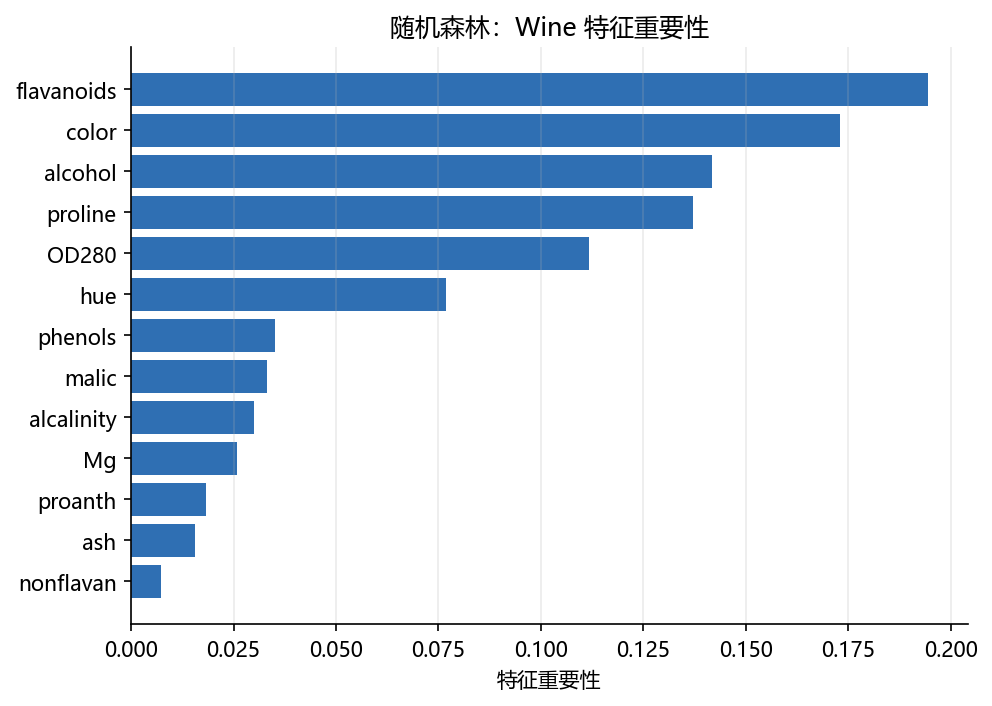
\includegraphics[keepaspectratio,alt={Wine 特征重要性}]{figures/08-sklearn/wine_feature_importance.png}}
\caption{Wine 特征重要性}
\end{figure}

\begin{quote}
黄酮（flavanoids）、颜色强度（color\_intensity）、酒精含量（alcohol）、脯氨酸（proline）等对品种区分贡献最大。这有助于我们``读懂''模型而不仅是得到一个分数。
\end{quote}

\subsection{第 4
步：无监督聚类（KMeans）}\label{ux7b2c-4-ux6b65ux65e0ux76d1ux7763ux805aux7c7bkmeans}

把``没有标签''的思路也用上：对标准化后的 Wine 做
KMeans，看能否大致还原真实品种。

\begin{Shaded}
\begin{Highlighting}[]
\ImportTok{from}\NormalTok{ sklearn.cluster }\ImportTok{import}\NormalTok{ KMeans}
\ImportTok{from}\NormalTok{ sklearn.metrics }\ImportTok{import}\NormalTok{ adjusted\_rand\_score, silhouette\_score}

\NormalTok{km }\OperatorTok{=}\NormalTok{ KMeans(n\_clusters}\OperatorTok{=}\DecValTok{3}\NormalTok{, random\_state}\OperatorTok{=}\DecValTok{42}\NormalTok{).fit(Xs)}
\BuiltInTok{print}\NormalTok{(}\StringTok{"轮廓系数:"}\NormalTok{, }\BuiltInTok{round}\NormalTok{(silhouette\_score(Xs, km.labels\_), }\DecValTok{4}\NormalTok{))}
\BuiltInTok{print}\NormalTok{(}\StringTok{"ARI vs 真实标签:"}\NormalTok{, }\BuiltInTok{round}\NormalTok{(adjusted\_rand\_score(y, km.labels\_), }\DecValTok{4}\NormalTok{))}
\BuiltInTok{print}\NormalTok{(}\StringTok{"各簇大小:"}\NormalTok{, np.bincount(km.labels\_))}
\end{Highlighting}
\end{Shaded}

\begin{Shaded}
\begin{Highlighting}[]
\NormalTok{轮廓系数: 0.2849}
\NormalTok{ARI vs 真实标签: 0.8975}
\NormalTok{各簇大小: [65 51 62]}
\end{Highlighting}
\end{Shaded}

\begin{quote}
\texttt{adjusted\_rand\_score=0.8975}
表示无监督聚类与真实品种高度一致（1 为完全一致），说明 Wine
数据确有明显的类结构。
\end{quote}

\subsection{第 5 步：PCA
降维并可视化}\label{ux7b2c-5-ux6b65pca-ux964dux7ef4ux5e76ux53efux89c6ux5316}

用 PCA 把 13 维压到 2 维，分别按真实类别与 KMeans 簇着色：

\begin{Shaded}
\begin{Highlighting}[]
\ImportTok{import}\NormalTok{ matplotlib.pyplot }\ImportTok{as}\NormalTok{ plt}
\NormalTok{plt.rcParams[}\StringTok{"font.sans{-}serif"}\NormalTok{] }\OperatorTok{=}\NormalTok{ [}\StringTok{"Microsoft YaHei"}\NormalTok{, }\StringTok{"SimHei"}\NormalTok{, }\StringTok{"DejaVu Sans"}\NormalTok{]}
\NormalTok{plt.rcParams[}\StringTok{"axes.unicode\_minus"}\NormalTok{] }\OperatorTok{=} \VariableTok{False}
\ImportTok{from}\NormalTok{ sklearn.decomposition }\ImportTok{import}\NormalTok{ PCA}

\NormalTok{pca }\OperatorTok{=}\NormalTok{ PCA(n\_components}\OperatorTok{=}\DecValTok{2}\NormalTok{)}
\NormalTok{Xp }\OperatorTok{=}\NormalTok{ pca.fit\_transform(Xs)}
\BuiltInTok{print}\NormalTok{(}\StringTok{"前两个主成分解释方差:"}\NormalTok{, np.}\BuiltInTok{round}\NormalTok{(pca.explained\_variance\_ratio\_, }\DecValTok{4}\NormalTok{))}
\BuiltInTok{print}\NormalTok{(}\StringTok{"累计解释方差:"}\NormalTok{, np.}\BuiltInTok{round}\NormalTok{(np.cumsum(pca.explained\_variance\_ratio\_), }\DecValTok{4}\NormalTok{))}

\NormalTok{fig, axes }\OperatorTok{=}\NormalTok{ plt.subplots(}\DecValTok{1}\NormalTok{, }\DecValTok{2}\NormalTok{, figsize}\OperatorTok{=}\NormalTok{(}\DecValTok{10}\NormalTok{, }\DecValTok{4}\NormalTok{))}
\NormalTok{axes[}\DecValTok{0}\NormalTok{].scatter(Xp[:, }\DecValTok{0}\NormalTok{], Xp[:, }\DecValTok{1}\NormalTok{], c}\OperatorTok{=}\NormalTok{y, cmap}\OperatorTok{=}\StringTok{"viridis"}\NormalTok{, s}\OperatorTok{=}\DecValTok{22}\NormalTok{)}
\NormalTok{axes[}\DecValTok{0}\NormalTok{].set\_title(}\StringTok{"PCA 按真实类别着色"}\NormalTok{)}
\NormalTok{axes[}\DecValTok{1}\NormalTok{].scatter(Xp[:, }\DecValTok{0}\NormalTok{], Xp[:, }\DecValTok{1}\NormalTok{], c}\OperatorTok{=}\NormalTok{km.labels\_, cmap}\OperatorTok{=}\StringTok{"viridis"}\NormalTok{, s}\OperatorTok{=}\DecValTok{22}\NormalTok{)}
\NormalTok{axes[}\DecValTok{1}\NormalTok{].set\_title(}\StringTok{"PCA 按 KMeans 簇着色"}\NormalTok{)}
\ControlFlowTok{for}\NormalTok{ ax }\KeywordTok{in}\NormalTok{ axes:}
\NormalTok{    ax.set\_xlabel(}\StringTok{"PC1"}\NormalTok{)}\OperatorTok{;}\NormalTok{ ax.set\_ylabel(}\StringTok{"PC2"}\NormalTok{)}\OperatorTok{;}\NormalTok{ ax.grid(alpha}\OperatorTok{=}\FloatTok{0.2}\NormalTok{)}
\NormalTok{fig.tight\_layout()}
\CommentTok{\#\# 图见 figures/08{-}sklearn/wine\_pca\_true\_vs\_kmeans.png}
\end{Highlighting}
\end{Shaded}

\begin{Shaded}
\begin{Highlighting}[]
\NormalTok{前两个主成分解释方差: [0.362  0.1921]}
\NormalTok{累计解释方差: [0.362  0.5541]}
\end{Highlighting}
\end{Shaded}

\begin{figure}
\centering
\pandocbounded{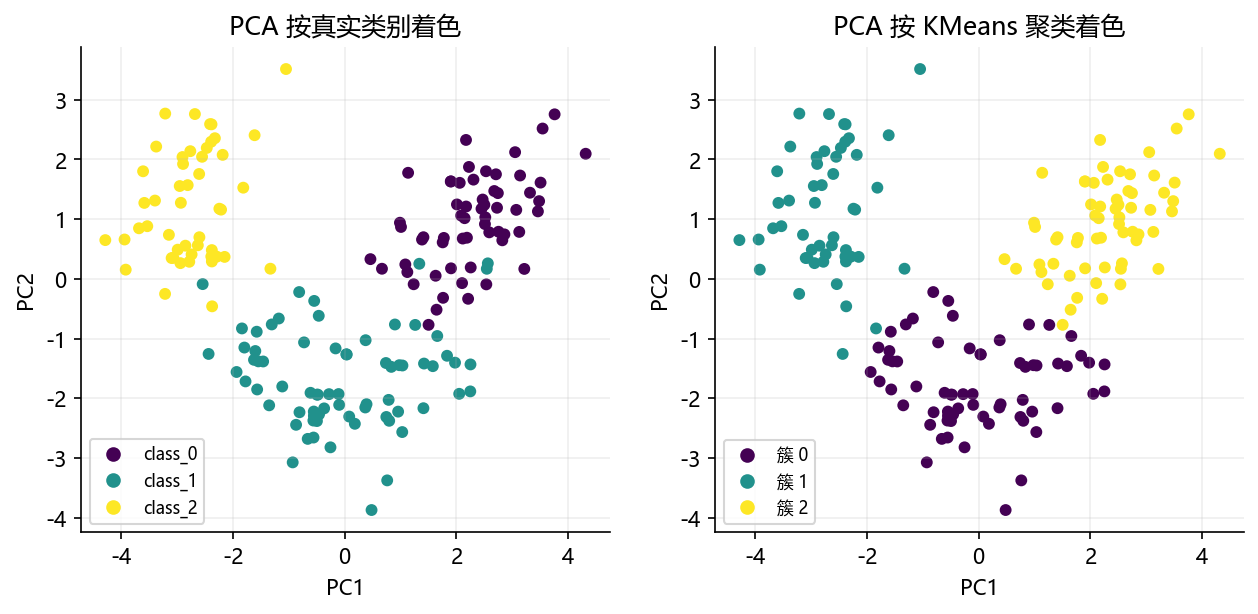
\includegraphics[keepaspectratio,alt={Wine PCA：真实类别 vs KMeans 簇}]{figures/08-sklearn/wine_pca_true_vs_kmeans.png}}
\caption{Wine PCA：真实类别 vs KMeans 簇}
\end{figure}

\begin{quote}
前两个主成分只保留约 55\% 方差，说明 13 维信息没有完全集中在 2
维，但散点已能看出三团结构；KMeans 簇与真实类别在 PCA 平面上也基本重合。
\end{quote}

\subsection{本章综合练习（上机任务）}\label{ux672cux7ae0ux7efcux5408ux7ec3ux4e60ux4e0aux673aux4efbux52a1-3}

\begin{enumerate}
\def\labelenumi{\arabic{enumi}.}
\tightlist
\item
  把本案例中的分类器换成
  \texttt{SVC}、\texttt{GradientBoostingClassifier}，比较 5 折均值。
\item
  用 \texttt{SelectKBest} 只保留前 5 个特征再分类，观察精度是否下降。
\item
  把 KMeans 的 \texttt{n\_clusters} 改为
  2、4、5，画出``k-ARI''曲线，解释最佳 k。
\item
  把 PCA 画成 2×2
  子图（PC1-PC2、PC1-PC3、PC2-PC3），观察哪个组合最易分。
\end{enumerate}

\subsection{延伸阅读}\label{ux5ef6ux4f38ux9605ux8bfb-37}

\begin{itemize}
\tightlist
\item
  sklearn 组合与
  Pipeline：https://scikit-learn.org/stable/modules/compose.html
\item
  sklearn
  特征重要性：https://scikit-learn.org/stable/modules/ensemble.html\#feature-importance
\item
  sklearn
  聚类评估（ARI/silhouette）：https://scikit-learn.org/stable/modules/clustering.html\#clustering-performance-evaluation
\end{itemize}

\section{05
常见误区与技巧}\label{ux5e38ux89c1ux8befux533aux4e0eux6280ux5de7-7}

\begin{quote}
本章新增``查漏补缺''页：把 sklearn
使用中最常见的坑集中列出，并给出性能、调试与自测清单。
\end{quote}

\subsection{1.
高频误区速查表}\label{ux9ad8ux9891ux8befux533aux901fux67e5ux8868-7}

{\def\LTcaptype{none} % do not increment counter
\begin{longtable}[]{@{}
  >{\raggedright\arraybackslash}p{(\linewidth - 6\tabcolsep) * \real{0.2500}}
  >{\raggedright\arraybackslash}p{(\linewidth - 6\tabcolsep) * \real{0.2500}}
  >{\raggedright\arraybackslash}p{(\linewidth - 6\tabcolsep) * \real{0.2500}}
  >{\raggedright\arraybackslash}p{(\linewidth - 6\tabcolsep) * \real{0.2500}}@{}}
\toprule\noalign{}
\begin{minipage}[b]{\linewidth}\raggedright
\#
\end{minipage} & \begin{minipage}[b]{\linewidth}\raggedright
误区 / 错误写法
\end{minipage} & \begin{minipage}[b]{\linewidth}\raggedright
正确做法
\end{minipage} & \begin{minipage}[b]{\linewidth}\raggedright
原因
\end{minipage} \\
\midrule\noalign{}
\endhead
\bottomrule\noalign{}
\endlastfoot
1 & \texttt{scaler.fit\_transform(X\_test)} & 训练集
\texttt{fit}，然后训练/测试都 \texttt{transform}；或用 \texttt{Pipeline}
& 用测试集统计量会``泄漏''测试信息 \\
2 & 对无序分类特征用 \texttt{LabelEncoder} & 用 \texttt{OneHotEncoder} /
\texttt{OrdinalEncoder} & 整数编码隐含顺序，误导模型 \\
3 & \texttt{r2\_score(y\_pred,\ y\_test)} &
\texttt{r2\_score(y\_test,\ y\_pred)} & 第一个参数是真值 y\_true \\
4 & 分类问题用 \texttt{r2\_score} & 用 \texttt{accuracy\_score} /
\texttt{f1\_score} / \texttt{roc\_auc\_score} & R² 只用于连续回归 \\
5 & \texttt{fit\_transform} 后再 \texttt{fit} 另一模型 & 把缩放放进
\texttt{Pipeline} 统一处理 & 避免重复/不一致的预处理 \\
6 & \texttt{load\_boston()} & 用 \texttt{load\_diabetes} /
\texttt{fetch\_california\_housing} / 自定义数据 & \texttt{load\_boston}
已在 sklearn 1.2 移除 \\
7 & \texttt{OneHotEncoder(sparse=False)} 老参数 &
\texttt{sparse\_output=False} & 新版本用 \texttt{sparse\_output} \\
8 & \texttt{RFE(estimator,\ 5)} 传位置参数 &
\texttt{RFE(estimator,\ n\_features\_to\_select=5)} & 新版
\texttt{n\_features\_to\_select} 是关键字参数 \\
9 & 用 \texttt{fit} 后直接 \texttt{transform} 新数据 & 先 \texttt{fit}
再 \texttt{transform}，否则 \texttt{NotFittedError} &
估计器必须携带训练统计量 \\
10 & \texttt{GridSearchCV} 不设 \texttt{random\_state} & 给模型与
\texttt{shuffle} 设置种子 & 结果不可复现 \\
11 & 对树模型也强制缩放 & 通常可跳过（缩放对树无益） &
树按阈值切分，不受量纲影响 \\
12 & \texttt{DBSCAN} 一个 \texttt{eps} 走天下 & 按数据量纲调
\texttt{eps}/\texttt{min\_samples} & 密度参数与数据尺度强相关 \\
13 & KMeans 不设 \texttt{random\_state} &
\texttt{KMeans(...,\ random\_state=0)} & 初始中心随机，结果不稳定 \\
14 & 用 \texttt{predict} 取概率 & 概率用
\texttt{predict\_proba}（二分类取 \texttt{{[}:,1{]}}） &
\texttt{predict} 返回类别标签 \\
15 & 混淆矩阵行/列方向记反 & 记住
\texttt{confusion\_matrix(y\_true,\ y\_pred)} 行是真值 &
行=真实，列=预测 \\
\end{longtable}
}

\subsection{2. 性能技巧}\label{ux6027ux80fdux6280ux5de7-6}

\begin{itemize}
\tightlist
\item
  \textbf{数据量优先用
  \texttt{n\_jobs=-1}}：\texttt{RandomForestClassifier(n\_jobs=-1)}、\texttt{GridSearchCV(...,\ n\_jobs=-1)}
  可并行（注意 RAM）。
\item
  \textbf{能向量化别循环}：特征处理尽量用 sklearn 方法一次性完成，避免
  Python 逐行 for。
\item
  \textbf{大矩阵用稀疏表示}：OneHot 后特征维度很大时保留稀疏矩阵（默认
  \texttt{sparse\_output=True}），别急着 \texttt{toarray()}。
\item
  \textbf{\texttt{Pipeline}
  更好维护}：把缩放、编码、特征选择、模型串成一个对象，训练/预测/调参都更安全。
\item
  \textbf{网格搜索先粗后细}：先搜大跨度，再在小范围精调；必要时用
  \texttt{RandomizedSearchCV} 代替 \texttt{GridSearchCV}。
\item
  \textbf{启用 Warm start}：增量训练可用 \texttt{partial\_fit}（如
  \texttt{SGDClassifier}）或 \texttt{warm\_start=True}（部分集成模型）。
\end{itemize}

\subsection{3. 调试建议}\label{ux8c03ux8bd5ux5efaux8bae-7}

\begin{enumerate}
\def\labelenumi{\arabic{enumi}.}
\tightlist
\item
  先打印
  \texttt{X.shape}、\texttt{y.shape}、\texttt{dtype}，确认维度与缺失值。
\item
  用 \texttt{np.isnan(X).sum()}、\texttt{np.isinf(X).sum()} 检查异常值。
\item
  出错先看 \textbf{fit 是否成功}：\texttt{model.fit(X,\ y)} 后打印
  \texttt{model.coef\_} / \texttt{model.feature\_importances\_}。
\item
  对 \texttt{Pipeline}，用 \texttt{pipe.named\_steps} 查看每一步；用
  \texttt{pipe.get\_params()} 检查参数名。
\item
  检查是否``数据泄漏''：

  \begin{itemize}
  \tightlist
  \item
    缩放器是否只 \texttt{fit} 在训练折（用 Pipeline 最保险）；
  \item
    \texttt{train\_test\_split} 是否在归一化之前。
  \end{itemize}
\item
  收敛警告（如``lbfgs failed to
  converge''）通常提示：特征未缩放、\texttt{max\_iter}
  太小，或类别不平衡。
\item
  固定所有随机种子（\texttt{random\_state}）并记录，便于复现与讨论。
\end{enumerate}

\subsection{4.
本章小结（自测）}\label{ux672cux7ae0ux5c0fux7ed3ux81eaux6d4b-4}

\begin{itemize}
\tightlist
\item[$\square$]
  能说清 \texttt{fit} / \texttt{transform} / \texttt{fit\_transform}
  的区别；
\item[$\square$]
  能用 Pipeline 做``缩放 + 模型''，避免数据泄漏；
\item[$\square$]
  能区分分类（准确率/F1/AUC）与回归（MSE/MAE/R²）指标；
\item[$\square$]
  能解释 \texttt{StandardScaler} 与 \texttt{MinMaxScaler} 的差异；
\item[$\square$]
  能比较 KMeans 与 DBSCAN 的适用场景；
\item[$\square$]
  能用 PCA / LDA 降到 2 维并读 \texttt{explained\_variance\_ratio\_}；
\item[$\square$]
  能独立完成 04 综合案例并写 3 句结论。
\end{itemize}

\subsection{延伸阅读}\label{ux5ef6ux4f38ux9605ux8bfb-38}

\begin{itemize}
\tightlist
\item
  sklearn API 速查：https://scikit-learn.org/stable/modules/classes.html
\item
  sklearn
  常见陷阱（用户指南）：https://scikit-learn.org/stable/modules/preprocessing.html
\item
  sklearn
  调试/性能相关：https://scikit-learn.org/stable/developers/performance.html
\end{itemize}

\backmatter

\appendix
%% 由 build/emit_tex.py 生成（生成物，勿手改）；定制请放 user_style.tex / user_meta.yaml
\chapter{线性代数与矩阵}\label{ux7ebfux6027ux4ee3ux6570ux4e0eux77e9ux9635}

\begin{quote}
本附录讲科学计算里最常用的线性代数：向量与矩阵是什么、怎么''想''它们、数字上怎么算、Python
里怎么调。学完你应能用''线性变换''的眼光看明白第 1 章 NumPy
的线性代数、第 8 章 sklearn 的降维。
\end{quote}

\begin{center}\rule{0.5\linewidth}{0.5pt}\end{center}

\section{A.1
直觉故事：矩阵到底在干什么}\label{a.1-ux76f4ux89c9ux6545ux4e8bux77e9ux9635ux5230ux5e95ux5728ux5e72ux4ec0ux4e48}

很多同学背熟了矩阵乘法，却不知道它''在算什么''。我们从一个具体问题开始：

\begin{quote}
一家店只卖两种套餐：A 套餐（米饭 1 份 + 鸡肉 2 份），B 套餐（米饭 2 份 +
鸡肉 1 份）。今天卖出 3 份 A、2 份 B，问一共用了多少米饭和鸡肉？
\end{quote}

把配额写成向量：卖出的数量 \texttt{x\ =\ (3,\ 2)}（A 份数、B
份数）。每种套餐的用料写成列向量：A 套餐 \texttt{(1,\ 2)}，B 套餐
\texttt{(2,\ 1)}。那么总用料就是\textbf{线性组合}：

\begin{Shaded}
\begin{Highlighting}[]
\NormalTok{总米饭 = 3×1 + 2×2 = 7；总鸡肉 = 3×2 + 2×1 = 8}
\NormalTok{→ 写成矩阵： [1 2; 2 1] × [3; 2] = [7; 8]}
\end{Highlighting}
\end{Shaded}

这个例子说明了三件事：

\begin{enumerate}
\def\labelenumi{\arabic{enumi}.}
\tightlist
\item
  \textbf{向量是''配比''}：一行数据、一份订单、一个状态，都可以是一个向量；
\item
  \textbf{矩阵是''线性变换的约定''}：\texttt{A}
  的每一列是一种''原料的配方''，\texttt{Ax} 就是按 \texttt{x}
  的比例把各列混合起来；
\item
  \textbf{矩阵乘法 = 复合变换}：先做变换再变换一次，顺序不能换------所以
  \texttt{AB\ ≠\ BA} 一般情况下成立。
\end{enumerate}

\textbf{为什么这对科学计算重要？}
因为很多模型都是一句''线性组合''：多项式拟合是''基函数的线性组合''、线性回归是''特征的线性组合''、傅里叶分析是''正弦波的线性组合''。学会线性代数，等于看懂了这些模型共同的骨架。

\begin{quote}
\textbf{正文见}：\href{../../chapters/01-numpy/03-线性代数.md}{1 NumPy ·
03
线性代数}（矩阵运算与求解）、\href{../../chapters/01-numpy/04-多项式与拟合.md}{1
NumPy · 04 多项式与拟合}（最小二乘）。
\end{quote}

\begin{center}\rule{0.5\linewidth}{0.5pt}\end{center}

\section{A.2
关键概念讲解：把名词翻译成人话}\label{a.2-ux5173ux952eux6982ux5ff5ux8bb2ux89e3ux628aux540dux8bcdux7ffbux8bd1ux6210ux4ebaux8bdd}

下面每个概念，先给定义，再用一句话人话解释，最后配一个 2×2 小例子。

\subsection{A.2.1
转置、内积与范数}\label{a.2.1-ux8f6cux7f6eux5185ux79efux4e0eux8303ux6570}

{\def\LTcaptype{none} % do not increment counter
\begin{longtable}[]{@{}lll@{}}
\toprule\noalign{}
概念 & 定义 & 人话 \\
\midrule\noalign{}
\endhead
\bottomrule\noalign{}
\endlastfoot
转置 \texttt{A\^{}T} & 行列互换 & ``把表格行变列、列变行'' \\
内积 \texttt{x·y\ =\ x\^{}T\ y} & 对应元素相乘再求和 &
``两个向量有多'同向''' \\
范数 \texttt{\textbar{}\textbar{}x\textbar{}\textbar{}\_2} &
\texttt{sqrt(x\^{}T\ x)} & ``向量长度'' \\
\end{longtable}
}

例子：\texttt{x\ =\ (1,\ 2)}，\texttt{y\ =\ (3,\ 4)}，则
\texttt{x·y\ =\ 1×3\ +\ 2×4\ =\ 11}，\texttt{\textbar{}\textbar{}x\textbar{}\textbar{}\_2\ =\ sqrt(1+4)\ ≈\ 2.24}。内积越大且同向，相似度越高------这就是余弦相似度、皮尔逊相关、注意力机制的底层直觉。

\subsection{A.2.2
逆、行列式与秩：能否把变换''倒回去''}\label{a.2.2-ux9006ux884cux5217ux5f0fux4e0eux79e9ux80fdux5426ux628aux53d8ux6362ux5012ux56deux53bb}

\begin{itemize}
\tightlist
\item
  \textbf{逆
  \texttt{A\^{}\{-1\}}}：把变换倒着做一遍。\texttt{A\^{}\{-1\}A\ =\ I}。
\item
  \textbf{行列式
  \texttt{det(A)}}：变换后''体积''放大的倍数。\texttt{det(A)\ =\ 0}
  表示变换把高维压扁了（不可逆），方程组要么无解要么无穷多解。
\item
  \textbf{秩
  \texttt{rank(A)}}：变换后空间的真正维度（列向量中线性无关的个数）。满秩方阵才可逆。
\end{itemize}

例子：\texttt{A\ =\ {[}{[}2,1{]},{[}1,2{]}{]}}。\texttt{det(A)\ =\ 4-1\ =\ 3\ ≠\ 0}，可逆；\texttt{A\^{}\{-1\}\ =\ (1/3){[}{[}2,-1{]},{[}-1,2{]}{]}}。而
\texttt{B\ =\ {[}{[}1,2{]},{[}2,4{]}{]}}
两列成比例，\texttt{rank(B)\ =\ 1}，\texttt{det(B)\ =\ 0}------它把平面压成一条线，因此
\texttt{Bx\ =\ b} 要么无解要么无穷多解。

\subsection{A.2.3
特征值与特征向量：变换的''不动轴''}\label{a.2.3-ux7279ux5f81ux503cux4e0eux7279ux5f81ux5411ux91cfux53d8ux6362ux7684ux4e0dux52a8ux8f74}

定义：若 \texttt{Av\ =\ λv}（\texttt{v\ ≠\ 0}），则 \texttt{v}
是特征向量，\texttt{λ}
是对应特征值。人话：\textbf{有的方向被矩阵只''拉伸''不''拐弯''，拉伸倍数是特征值}。

继续用 \texttt{A\ =\ {[}{[}2,1{]},{[}1,2{]}{]}}：特征值
\texttt{λ1\ =\ 3}（方向 \texttt{(1,1)}）、\texttt{λ2\ =\ 1}（方向
\texttt{(1,-1)}）。也就是说：沿对角线方向放 3 倍、沿反对角线方向不动。

用处： - 对称矩阵
\texttt{A\ =\ QΛQ\^{}T}：把坐标轴转成''特征方向''，问题立刻解耦（PCA
就是找这些方向）； -
幂迭代、PageRank、马尔可夫链稳态都在找''最大特征值的特征向量''。

\subsection{A.2.4
条件数：解的''敏感度''}\label{a.2.4-ux6761ux4ef6ux6570ux89e3ux7684ux654fux611fux5ea6}

\texttt{cond(A)\ =\ \textbar{}\textbar{}A\textbar{}\textbar{}\ ·\ \textbar{}\textbar{}A\^{}\{-1\}\textbar{}\textbar{}}，粗略说明：\texttt{b}
变化一点点，\texttt{x} 可能变化多大倍数。条件数大（病态）≠
无解，而是\textbf{数值上很难算准}。

\begin{quote}
\textbf{正文见}：\href{../../chapters/01-numpy/03-线性代数.md}{1 NumPy ·
03
线性代数}（条件数/病态）、\href{../../chapters/03-scipy/02-优化工具包.md}{3
SciPy · 02 优化工具包}（优化里的病态）。
\end{quote}

\begin{center}\rule{0.5\linewidth}{0.5pt}\end{center}

\section{A.3
分解与算法：为什么这样做}\label{a.3-ux5206ux89e3ux4e0eux7b97ux6cd5ux4e3aux4ec0ux4e48ux8fd9ux6837ux505a}

\subsection{A.3.1 解方程组：从高斯消元到
LU}\label{a.3.1-ux89e3ux65b9ux7a0bux7ec4ux4eceux9ad8ux65afux6d88ux5143ux5230-lu}

求解 \texttt{Ax\ =\ b}
最直接是高斯消元：把增广矩阵化成上三角，再回代。消元过程等价于把
\texttt{A} 写成 \texttt{A\ =\ LU}（L 下三角、U
上三角）。好处是：\textbf{解多组 \texttt{b} 时复用
LU，一次消元多次求解}。

\begin{itemize}
\tightlist
\item
  矩阵规模 \texttt{n×n}，复杂度 \texttt{O(n\^{}3)}；
\item
  数值上要\textbf{部分主元}（选最大的元素当主元），避免小除数放大误差；
\item
  Python 里直接 \texttt{np.linalg.solve}（内部就是带主元的
  LU），\textbf{不要}用 \texttt{inv(A)\ @\ b}。
\end{itemize}

\subsection{A.3.2 特征值分解与
SVD：谁是''最重要的方向''}\label{a.3.2-ux7279ux5f81ux503cux5206ux89e3ux4e0e-svdux8c01ux662fux6700ux91cdux8981ux7684ux65b9ux5411}

\begin{itemize}
\tightlist
\item
  \textbf{特征分解}：\texttt{A\ =\ VΛV\^{}\{-1\}}（对称阵时 \texttt{V}
  正交，\texttt{A\ =\ QΛQ\^{}T}）。适合方阵、可对角化矩阵；求
  \texttt{A\^{}k}、判断稳态很舒服。
\item
  \textbf{奇异值分解
  SVD}：\texttt{A\ =\ UΣV\^{}T}，\textbf{任意矩阵都行}。\texttt{U}、\texttt{V}
  正交，\texttt{Σ}
  对角（奇异值按降序）。直觉：把''变换''分解成''先旋转、再缩放、再旋转''。
\end{itemize}

SVD 最漂亮的性质是\textbf{最优低秩近似}（Eckart--Young）：保留前
\texttt{k} 大奇异值，就得到与原矩阵''最接近''的秩 \texttt{k}
矩阵。所以： - 图像压缩：把大矩阵拆成''少数奇异值 × 两个小矩阵''； -
PCA：对数据矩阵做 SVD，右奇异向量就是主成分方向； -
伪逆与最小二乘：\texttt{A\^{}+\ =\ VΣ\^{}\{-1\}U\^{}T}，比正规方程稳定。

\begin{quote}
\textbf{正文见}：\href{../../chapters/01-numpy/05-综合案例.md}{1 NumPy ·
05 综合案例}（SVD
图像压缩）、\href{../../chapters/08-sklearn/03-无监督学习的案例.md}{8
sklearn · 03 无监督学习的案例}（PCA 降维）。
\end{quote}

\subsection{A.3.3
最小二乘：数据有噪声怎么办}\label{a.3.3-ux6700ux5c0fux4e8cux4e58ux6570ux636eux6709ux566aux58f0ux600eux4e48ux529e}

超定方程
\texttt{Ax\ ≈\ b}（方程比未知数多）通常无精确解，最小二乘找''残差平方和最小''的解：

\begin{Shaded}
\begin{Highlighting}[]
\NormalTok{正规方程：x\^{} = (A\^{}T A)\^{}\{{-}1\} A\^{}T b}
\NormalTok{几何：    把 b 投影到 A 的列空间，误差向量垂直于列空间}
\NormalTok{数值：    优先 lstsq（QR/ SVD 路径），避免求 (A\^{}T A)\^{}\{{-}1\}（会平方条件数）}
\end{Highlighting}
\end{Shaded}

如果再加 \texttt{\textbar{}\textbar{}x\textbar{}\textbar{}\^{}2}
惩罚（岭回归），就是''在最小二乘和'不放大'之间妥协''------这是第 8
章正则化的数学原型。

\begin{center}\rule{0.5\linewidth}{0.5pt}\end{center}

\section{A.4 Python
对应（速查）}\label{a.4-python-ux5bf9ux5e94ux901fux67e5}

\begin{Shaded}
\begin{Highlighting}[]
\ImportTok{import}\NormalTok{ numpy }\ImportTok{as}\NormalTok{ np, sympy }\ImportTok{as}\NormalTok{ sp}

\NormalTok{A }\OperatorTok{=}\NormalTok{ np.array([[}\DecValTok{2}\NormalTok{, }\DecValTok{1}\NormalTok{], [}\DecValTok{1}\NormalTok{, }\DecValTok{2}\NormalTok{]])}
\NormalTok{b }\OperatorTok{=}\NormalTok{ np.array([[}\DecValTok{1}\NormalTok{], [}\DecValTok{2}\NormalTok{]])}

\NormalTok{np.linalg.solve(A, b)                 }\CommentTok{\# 解方程组（推荐）}
\NormalTok{np.linalg.inv(A)                      }\CommentTok{\# 显式求逆（尽量不用）}
\NormalTok{np.linalg.det(A), np.linalg.matrix\_rank(A)}
\NormalTok{np.linalg.eig(A)                      }\CommentTok{\# 特征值/特征向量}
\NormalTok{np.linalg.eigh(A) }\ControlFlowTok{if}\NormalTok{ (A }\OperatorTok{==}\NormalTok{ A.T).}\BuiltInTok{all}\NormalTok{() }\ControlFlowTok{else} \VariableTok{None}   \CommentTok{\# 对称矩阵专用}
\NormalTok{np.linalg.svd(A, full\_matrices}\OperatorTok{=}\VariableTok{False}\NormalTok{)  }\CommentTok{\# U, S, Vt（S 是向量!）}
\NormalTok{np.linalg.lstsq(A, b, rcond}\OperatorTok{=}\VariableTok{None}\NormalTok{)      }\CommentTok{\# 最小二乘}
\NormalTok{np.linalg.cond(A)                      }\CommentTok{\# 条件数}
\NormalTok{np.linalg.pinv(A)                      }\CommentTok{\# 伪逆}

\CommentTok{\# SymPy 符号解}
\NormalTok{sp.Matrix([[}\DecValTok{2}\NormalTok{,}\DecValTok{1}\NormalTok{],[}\DecValTok{1}\NormalTok{,}\DecValTok{2}\NormalTok{]]).eigenvects()}
\end{Highlighting}
\end{Shaded}

{\def\LTcaptype{none} % do not increment counter
\begin{longtable}[]{@{}ll@{}}
\toprule\noalign{}
你想要 & 用哪个 \\
\midrule\noalign{}
\endhead
\bottomrule\noalign{}
\endlastfoot
解方阵方程组 & \texttt{np.linalg.solve} \\
最小二乘 & \texttt{np.linalg.lstsq} \\
特征值（对称） & \texttt{np.linalg.eigh} \\
SVD & \texttt{np.linalg.svd}（注意 \texttt{S} 是向量） \\
判断病态 & \texttt{np.linalg.cond} \\
\end{longtable}
}

\begin{center}\rule{0.5\linewidth}{0.5pt}\end{center}

\section{A.5 动手例题（选做：手算 +
验证）}\label{a.5-ux52a8ux624bux4f8bux9898ux9009ux505aux624bux7b97-ux9a8cux8bc1}

\textbf{例 1：解方程组}。解 @BT@2x + y = 1@BT@、@BT@x + 2y =
2@BT@。手算：由第一式 @BT@y = 1 - 2x@BT@ 代入第二式 @BT@x + 2(1-2x) =
2@BT@ → @BT@-3x = 0@BT@ → @BT@x = 0@BT@，@BT@y =
1@BT@。代码验证：@BT@np.linalg.solve({[}{[}2,1{]},{[}1,2{]}{]},
{[}1,2{]}) = {[}0, 1{]}@BT@。

\textbf{例 2：最小二乘的''投影直觉''}。数据 @BT@(0,1), (1,2), (2,3)@BT@
明显在同一直线 @BT@y = x + 1@BT@ 上，最小二乘应还原出斜率 1、截距
1。若把第 3 点改成 @BT@(2, 4)@BT@（有噪声），斜率会略大于
1------因为解被''拉''向那个异常点。试试：

\begin{Shaded}
\begin{Highlighting}[]
\ImportTok{import}\NormalTok{ numpy }\ImportTok{as}\NormalTok{ np}
\NormalTok{x }\OperatorTok{=}\NormalTok{ np.array([}\FloatTok{0.}\NormalTok{, }\FloatTok{1.}\NormalTok{, }\FloatTok{2.}\NormalTok{])}\OperatorTok{;}\NormalTok{ y }\OperatorTok{=}\NormalTok{ np.array([}\FloatTok{1.}\NormalTok{, }\FloatTok{2.}\NormalTok{, }\FloatTok{3.}\NormalTok{])}
\NormalTok{A }\OperatorTok{=}\NormalTok{ np.vstack([x, np.ones\_like(x)]).T        }\CommentTok{\# 列：[x, 1]}
\NormalTok{k, b }\OperatorTok{=}\NormalTok{ np.linalg.lstsq(A, y, rcond}\OperatorTok{=}\VariableTok{None}\NormalTok{)[}\DecValTok{0}\NormalTok{]}
\BuiltInTok{print}\NormalTok{(k, b)                                   }\CommentTok{\# 1.0 1.0}
\NormalTok{y2 }\OperatorTok{=}\NormalTok{ np.array([}\FloatTok{1.}\NormalTok{, }\FloatTok{2.}\NormalTok{, }\FloatTok{4.}\NormalTok{])}
\BuiltInTok{print}\NormalTok{(np.linalg.lstsq(A, y2, rcond}\OperatorTok{=}\VariableTok{None}\NormalTok{)[}\DecValTok{0}\NormalTok{])  }\CommentTok{\# 斜率 \textgreater{} 1，被噪声拉偏}
\end{Highlighting}
\end{Shaded}

\section{A.6 常见误区 +
用在哪（双向）}\label{a.6-ux5e38ux89c1ux8befux533a-ux7528ux5728ux54eaux53ccux5411}

{\def\LTcaptype{none} % do not increment counter
\begin{longtable}[]{@{}ll@{}}
\toprule\noalign{}
误区 & 正确 \\
\midrule\noalign{}
\endhead
\bottomrule\noalign{}
\endlastfoot
\texttt{A\ *\ B} 当矩阵乘 & \texttt{*} 是逐元素；用 \texttt{A\ @\ B} \\
用 \texttt{inv(A)\ @\ b} & 用 \texttt{solve} / \texttt{lstsq} \\
以为 \texttt{S} 是矩阵 & SVD 返回奇异值\textbf{向量}，需
\texttt{np.diag(S)} \\
忽略条件数 & 病态时解会''抖''，先看 \texttt{cond} \\
非对称矩阵用 \texttt{eigh} & \texttt{eigh} 要求对称；否则用
\texttt{eig} \\
\end{longtable}
}

\textbf{使用章节（可点击）} \textbar{} 章 \textbar{} 哪里用到 \textbar{}
链接 \textbar{} \textbar{} ---- \textbar{} ---- \textbar{} ----
\textbar{} \textbar{} 1 NumPy \textbar{} 03 线性代数、05 SVD 压缩
\textbar{} \href{../../chapters/01-numpy/03-线性代数.md}{正文}
\textbar{} \textbar{} 2 SymPy \textbar{} 矩阵与特征值 \textbar{}
\href{../../chapters/02-sympy/01-符号对象与基本运算.md}{正文} \textbar{}
\textbar{} 3 SciPy \textbar{} 优化/插值中的矩阵 \textbar{}
\href{../../chapters/03-scipy/02-优化工具包.md}{正文} \textbar{}
\textbar{} 8 sklearn \textbar{} PCA/降维 \textbar{}
\href{../../chapters/08-sklearn/03-无监督学习的案例.md}{正文} \textbar{}

\textbf{下游衔接}：intro-mathmodel 第 1 章（Numpy 与线性代数）、第 3
章（线性规划→非线性规划）。 \textbf{延伸阅读}：mml-book 第
2\textasciitilde4 章、SciPy Lectures、numpy.linalg 官方文档（见
\href{./references.md}{本目录 references.md}）。

\begin{center}\rule{0.5\linewidth}{0.5pt}\end{center}

\section{A.7 补充：特征值与 SVD 的 3
个实际用途}\label{a.7-ux8865ux5145ux7279ux5f81ux503cux4e0e-svd-ux7684-3-ux4e2aux5b9eux9645ux7528ux9014}

\begin{enumerate}
\def\labelenumi{\arabic{enumi}.}
\tightlist
\item
  \textbf{收敛性判断（马尔可夫链/PageRank）}：状态转移矩阵的最大特征值决定系统是否收敛到稳态；PageRank
  就是求转移矩阵最大特征值的特征向量（幂迭代）。
\item
  \textbf{去噪与压缩（SVD）}：保留前 k 个奇异值 =
  丢掉''不重要的方向''。对一张 100×100 的图，只保留前 10
  个奇异值，视觉上几乎一样，但数据量从 10000 降到约 2100。
\item
  \textbf{求逆与最小二乘（伪逆）}：@BT@A\^{}+ =
  VΣ\textsuperscript{\{-1\}U}T@BT@ 对任意矩阵（含奇异）都定义良好，是
  @BT@lstsq@BT@ 的底层路径。
\end{enumerate}

\textbf{一句话总结}：特征值/奇异值大小 =
该方向的重要程度；``取前几个''就是''保留主要信息，丢弃噪声''。

%% 由 build/emit_tex.py 生成（生成物，勿手改）；定制请放 user_style.tex / user_meta.yaml
\chapter{微积分与数值方法}\label{ux5faeux79efux5206ux4e0eux6570ux503cux65b9ux6cd5}

\begin{quote}
一句话：微积分研究''变化与累积''，数值方法回答''电脑上怎么算''。本章覆盖导数/积分直觉、数值微分积分、插值、优化、傅里叶与常微分方程。
\end{quote}

\section{B.1
直觉：导数、积分与泰勒}\label{b.1-ux76f4ux89c9ux5bfcux6570ux79efux5206ux4e0eux6cf0ux52d2}

\begin{itemize}
\tightlist
\item
  \textbf{导数}：瞬时变化率（\texttt{f\textquotesingle{}(x)\ =\ lim\ dx→0\ (f(x+dx)-f(x))/dx}）；梯度把导数推广到多元：\texttt{grad\ f\ =\ (∂f/∂x1,\ …,\ ∂f/∂xn)}
  指向上升最快的方向。
\item
  \textbf{积分}：累积量（面积/总量）；\texttt{∫\_a\^{}b\ f(x)\ dx}
  与导数是互逆（微积分基本定理）。
\item
  \textbf{泰勒展开}：\texttt{f(x+h)\ ≈\ f(x)\ +\ f\textquotesingle{}(x)h\ +\ f\textquotesingle{}\textquotesingle{}(x)h²/2\ +\ …}------把非线性函数局部''线性化''（后文牛顿法/误差分析都用它）。
\end{itemize}

\section{B.2
关键公式速查}\label{b.2-ux5173ux952eux516cux5f0fux901fux67e5}

{\def\LTcaptype{none} % do not increment counter
\begin{longtable}[]{@{}
  >{\raggedright\arraybackslash}p{(\linewidth - 4\tabcolsep) * \real{0.3333}}
  >{\raggedright\arraybackslash}p{(\linewidth - 4\tabcolsep) * \real{0.3333}}
  >{\raggedright\arraybackslash}p{(\linewidth - 4\tabcolsep) * \real{0.3333}}@{}}
\toprule\noalign{}
\begin{minipage}[b]{\linewidth}\raggedright
主题
\end{minipage} & \begin{minipage}[b]{\linewidth}\raggedright
公式/结论
\end{minipage} & \begin{minipage}[b]{\linewidth}\raggedright
用途
\end{minipage} \\
\midrule\noalign{}
\endhead
\bottomrule\noalign{}
\endlastfoot
微分 &
\texttt{(x\^{}n)\textquotesingle{}\ =\ n\ x\^{}\{n-1\}}、\texttt{(sin\ x)\textquotesingle{}\ =\ cos\ x}、\texttt{(e\^{}x)\textquotesingle{}\ =\ e\^{}x}
& 手算/校验 \\
链式 &
\texttt{(f(g(x)))\textquotesingle{}\ =\ f\textquotesingle{}(g(x))\ g\textquotesingle{}(x)}
& 反向传播 \\
梯度 & \texttt{grad\ f}；方向导数在梯度方向最大 & 梯度下降 \\
泰勒 & 一阶/二阶近似 & 牛顿法、误差界 \\
积分 & 基本定理、分部积分 & 概率期望/总面积 \\
数值积分 & 梯形 \texttt{≈\ (b-a)(f(a)+f(b))/2}；辛普森更高阶 &
无解析积分时 \\
数值微分 & 中心差分 \texttt{(f(x+h)-f(x-h))/(2h)} &
无公式时/\texttt{SciPy.optimize}内部 \\
\end{longtable}
}

\section{B.3
数值方法：算法思路}\label{b.3-ux6570ux503cux65b9ux6cd5ux7b97ux6cd5ux601dux8def}

\subsection{B.3.1
数值积分与微分}\label{b.3.1-ux6570ux503cux79efux5206ux4e0eux5faeux5206}

\begin{itemize}
\tightlist
\item
  把 \texttt{{[}a,b{]}}
  分块，块内用低阶多项式近似：梯形（一阶）、辛普森（二阶）、高斯求积（自适应）；误差与步长
  \texttt{h} 的幂有关。
\item
  数值微分怕噪声：慎用；需要时用中心差分或拟合后求导（\texttt{np.polyfit}→\texttt{np.polyder}）。
\end{itemize}

\subsection{B.3.2
优化（求极值）}\label{b.3.2-ux4f18ux5316ux6c42ux6781ux503c}

{\def\LTcaptype{none} % do not increment counter
\begin{longtable}[]{@{}lll@{}}
\toprule\noalign{}
方法 & 思想 & 适用 \\
\midrule\noalign{}
\endhead
\bottomrule\noalign{}
\endlastfoot
梯度下降 & 沿负梯度迭代：\texttt{x\ ←\ x\ -\ α·grad\ f(x)} &
大模型/无二阶信息 \\
牛顿法 & 用二阶泰勒：\texttt{x\ ←\ x\ -\ H\^{}\{-1\}·grad\ f} &
二阶信息可用时收敛快 \\
拟牛顿/BFGS & 近似 \texttt{H\^{}\{-1\}} &
中规模、\texttt{scipy.optimize.minimize} 默认 \\
约束优化 & \texttt{min\ f(x)\ s.t.\ g(x)≤0} & 拉格朗日/KKT 条件 \\
\end{longtable}
}

\begin{quote}
收敛性：凸函数梯度下降线性收敛；牛顿法（好初值）二次收敛。\textbf{初值很关键}。
\end{quote}

\subsection{B.3.3
插值与拟合}\label{b.3.3-ux63d2ux503cux4e0eux62dfux5408}

\begin{itemize}
\tightlist
\item
  \textbf{插值}：曲线\textbf{穿过}所有数据点（拉格朗日/样条）；高次可能震荡（龙格现象）。
\item
  \textbf{拟合（最小二乘）}：曲线\textbf{逼近}数据（不要求穿过）；由附录
  A 的 \texttt{lstsq} 实现。
\item
  选择：噪声大→拟合；数据精确且要过点→样条插值。
\end{itemize}

\subsection{B.3.4
傅里叶变换（FFT）}\label{b.3.4-ux5085ux91ccux53f6ux53d8ux6362fft}

\begin{itemize}
\tightlist
\item
  把信号分解为不同频率的正弦波叠加：\texttt{X(k)\ =\ Σ\ x(n)\ e\^{}\{-2πikn/N\}}；
\item
  FFT 复杂度
  \texttt{O(N\ log\ N)}；看频谱找周期、滤波、平滑（\texttt{scipy.fft\ /\ np.fft}）。
\end{itemize}

\subsection{B.3.5
常微分方程（ODE）}\label{b.3.5-ux5e38ux5faeux5206ux65b9ux7a0bode}

\begin{itemize}
\tightlist
\item
  初值问题
  \texttt{y\textquotesingle{}\ =\ f(t,y),\ y(t0)=y0}：数值解按步长推进（欧拉、RK45
  等）；
\item
  \texttt{scipy.integrate.solve\_ivp} 自动选步长；符号精确解用 SymPy
  \texttt{dsolve}。
\end{itemize}

\section{B.4 Python 对应}\label{b.4-python-ux5bf9ux5e94}

\begin{Shaded}
\begin{Highlighting}[]
\ImportTok{import}\NormalTok{ numpy }\ImportTok{as}\NormalTok{ np, scipy.integrate }\ImportTok{as}\NormalTok{ si, scipy.optimize }\ImportTok{as}\NormalTok{ so}
\ImportTok{from}\NormalTok{ scipy }\ImportTok{import}\NormalTok{ interpolate, fft}

\CommentTok{\# 数值积分/微分}
\NormalTok{si.quad(np.sin, }\DecValTok{0}\NormalTok{, np.pi)          }\CommentTok{\# 数值积分}
\NormalTok{np.gradient(np.array([}\DecValTok{0}\NormalTok{, }\DecValTok{1}\NormalTok{, }\DecValTok{4}\NormalTok{, }\DecValTok{9}\NormalTok{]), }\FloatTok{0.1}\NormalTok{)   }\CommentTok{\# 数值微分（中心差分）}

\CommentTok{\# 优化}
\NormalTok{so.minimize(}\KeywordTok{lambda}\NormalTok{ x: (x[}\DecValTok{0}\NormalTok{]}\OperatorTok{{-}}\DecValTok{2}\NormalTok{)}\OperatorTok{**}\DecValTok{2} \OperatorTok{+}\NormalTok{ (x[}\DecValTok{1}\NormalTok{]}\OperatorTok{+}\DecValTok{1}\NormalTok{)}\OperatorTok{**}\DecValTok{2}\NormalTok{, x0}\OperatorTok{=}\NormalTok{[}\DecValTok{0}\NormalTok{, }\DecValTok{0}\NormalTok{])   }\CommentTok{\# BFGS}

\CommentTok{\# 插值/拟合}
\NormalTok{interpolate.interp1d(x, y, kind}\OperatorTok{=}\StringTok{"cubic"}\NormalTok{)}
\NormalTok{np.polyfit(x, y, }\DecValTok{2}\NormalTok{)}

\CommentTok{\# FFT / ODE}
\NormalTok{fft.fft(signal)}
\NormalTok{si.solve\_ivp(}\KeywordTok{lambda}\NormalTok{ t, y: }\OperatorTok{{-}}\NormalTok{y, [}\DecValTok{0}\NormalTok{, }\DecValTok{5}\NormalTok{], [}\FloatTok{1.0}\NormalTok{])   }\CommentTok{\# y\textquotesingle{} = {-}y}
\end{Highlighting}
\end{Shaded}

\section{B.5 常见误区}\label{b.5-ux5e38ux89c1ux8befux533a}

{\def\LTcaptype{none} % do not increment counter
\begin{longtable}[]{@{}ll@{}}
\toprule\noalign{}
误区 & 正确 \\
\midrule\noalign{}
\endhead
\bottomrule\noalign{}
\endlastfoot
插值=拟合 & 插值过点、拟合逼近；数据有噪声用拟合 \\
优化不设初值 & 非凸问题初值决定结果；多试几个/给定范围 \\
数值微分会放大噪声 & 先平滑/拟合，再求导；或改用解析导数 \\
以为 FFT 只用于音频 & 任何周期信号/时间序列都能看频谱 \\
用默认 ODE 求解器硬解刚性问题 & 选 \texttt{method="Radau"} 等刚性方法 \\
\end{longtable}
}

\section{B.6
使用章节与下游衔接}\label{b.6-ux4f7fux7528ux7ae0ux8282ux4e0eux4e0bux6e38ux8854ux63a5}

\begin{itemize}
\tightlist
\item
  章节：2 SymPy（极限/导数/积分/方程/ODE）、3
  SciPy（积分/优化/插值/FFT/ODE）、1 NumPy（多项式拟合）；
\item
  下游：intro-mathmodel 第 2 章（微分方程与动力系统）、第 3
  章（函数极值与规划模型）、第 6 章（数据处理与拟合模型）；
\item
  参考：SciPy Lectures 优化与积分、MIT OCW
  数值计算、中文《数值分析》（见 references.md）。
\end{itemize}

%% 由 build/emit_tex.py 生成（生成物，勿手改）；定制请放 user_style.tex / user_meta.yaml
\chapter{概率统计基础}\label{ux6982ux7387ux7edfux8ba1ux57faux7840}

\begin{quote}
一句话：概率给''不确定性''建模，统计从数据里''猜''出规律。本附录覆盖描述统计、常用分布、推断（检验/置信区间）、回归与时间序列。
\end{quote}

\section{C.1
直觉与描述统计}\label{c.1-ux76f4ux89c9ux4e0eux63cfux8ff0ux7edfux8ba1}

\begin{itemize}
\tightlist
\item
  \textbf{随机变量}：取值带概率的变量。期望 \texttt{E{[}X{]}} =
  中心位置；方差 \texttt{Var(X)\ =\ E{[}(X-E{[}X{]})²{]}} = 分散程度。
\item
  \textbf{样本统计量}：从数据算出来的''估计''------均值、中位数、标准差、分位数、相关系数。
\item
  \textbf{为什么先看分布}：均值会被极端值拉偏；分布形状（偏斜/厚尾）决定该用哪种方法。
\end{itemize}

常用量速查：

{\def\LTcaptype{none} % do not increment counter
\begin{longtable}[]{@{}lll@{}}
\toprule\noalign{}
量 & 定义 & 说明 \\
\midrule\noalign{}
\endhead
\bottomrule\noalign{}
\endlastfoot
均值 \texttt{μ\^{}\ =\ (1/n)Σx\_i} & 集中趋势 & 受异常值影响 \\
中位数 & 排序中间值 & 稳健 \\
方差/标准差 & \texttt{s²\ =\ Σ(x\_i\ -\ x̄)²/(n-1)} & 离散程度（样本用
n-1） \\
协方差/相关 & \texttt{Cov(X,Y)}、\texttt{ρ\ =\ Cov/(σx\ σy)} &
线性相关方向/强度 \\
分位数 & 排序后百分比位置 & Q1/Q3/IQR（箱线图） \\
\end{longtable}
}

\section{C.2
常用分布速查}\label{c.2-ux5e38ux7528ux5206ux5e03ux901fux67e5}

{\def\LTcaptype{none} % do not increment counter
\begin{longtable}[]{@{}lll@{}}
\toprule\noalign{}
分布 & 记号 & 用在哪 \\
\midrule\noalign{}
\endhead
\bottomrule\noalign{}
\endlastfoot
正态 & \texttt{N(μ,\ σ²)} & 近似很多现象；中心极限定理的主角 \\
二项 & \texttt{B(n,\ p)} & 成功/失败次数 \\
泊松 & \texttt{Poisson(λ)} & 一段时间内事件数 \\
均匀 & \texttt{U(a,\ b)} & 随机数/先验 \\
t / F / χ² & \texttt{t(n)}, \texttt{F}, \texttt{χ²} &
小样本推断/方差分析 \\
\end{longtable}
}

\begin{quote}
\textbf{中心极限定理}：大量独立同分布随机变量的均值，近似正态分布------这是很多统计方法（包括回归的置信区间）的底气。
\end{quote}

\section{C.3
统计推断：检验与置信区间}\label{c.3-ux7edfux8ba1ux63a8ux65adux68c0ux9a8cux4e0eux7f6eux4fe1ux533aux95f4}

\begin{itemize}
\tightlist
\item
  \textbf{参数估计}：点估计（均值）→
  区间估计（置信区间：\texttt{x̄\ ±\ t\_\{α/2\}·s/√n}）。
\item
  \textbf{假设检验}：先立原假设 \texttt{H0}（如''均值=0''），看数据在
  \texttt{H0} 下多''极端''（p 值）；\texttt{p\ \textless{}\ 0.05} → 拒绝
  \texttt{H0}。
\item
  \textbf{两类错误}：第一类（误拒，α）、第二类（漏拒，β）；功效 = 1-β。
\item
  \textbf{常见检验}：t
  检验（均值）、卡方（拟合/列联）、F/ANOVA（多组均值）、KS（分布）。
\item
  \textbf{重要提醒}：p 值小 ≠ 实际重要；报告效应量 + 置信区间。
\end{itemize}

\section{C.4
回归与方差分析（建模视角）}\label{c.4-ux56deux5f52ux4e0eux65b9ux5deeux5206ux6790ux5efaux6a21ux89c6ux89d2}

\begin{itemize}
\tightlist
\item
  \textbf{线性回归}：\texttt{y\ =\ β0\ +\ β1x1\ +\ …\ +\ ε}；OLS
  最小化残差平方和（附录 A 最小二乘）。
\item
  \textbf{假设}：线性、独立、同方差、正态（对推断）；违背时用稳健标准误/变换。
\item
  \textbf{\texttt{R²}}：解释变量能解释的变异比例（\texttt{R²\ =\ 1\ -\ SSE/SST}），过大要提防过拟合。
\item
  \textbf{ANOVA}：检验多个组的均值是否相等（\texttt{F}
  检验，组间方差/组内方差）。
\item
  \textbf{逻辑回归}：把线性预测过 sigmoid
  映射成概率：\texttt{P(y=1)\ =\ σ(β\^{}T\ x)}；损失用交叉熵（与附录 E
  衔接）。
\end{itemize}

\section{C.5
时间序列基础}\label{c.5-ux65f6ux95f4ux5e8fux5217ux57faux7840}

{\def\LTcaptype{none} % do not increment counter
\begin{longtable}[]{@{}lll@{}}
\toprule\noalign{}
概念 & 直觉 & 常用工具 \\
\midrule\noalign{}
\endhead
\bottomrule\noalign{}
\endlastfoot
平稳性 & 统计特性不随时间漂移 & 单位根检验（ADF） \\
自相关/ACF & 与过去的相关 & 确定滞后阶数 \\
差分 & \texttt{y\_t\ -\ y\_\{t-1\}} 消除趋势 & 转平稳 \\
移动平均/平滑 & 去噪/看趋势 & \texttt{rolling} \\
分解 & 趋势 + 季节 + 残差 & \texttt{seasonal\_decompose} \\
ARIMA & AR（自回归）+ I（差分）+ MA（移动平均误差） & 预测/理解 \\
\end{longtable}
}

\section{C.6 Python 对应}\label{c.6-python-ux5bf9ux5e94}

\begin{Shaded}
\begin{Highlighting}[]
\ImportTok{import}\NormalTok{ numpy }\ImportTok{as}\NormalTok{ np, pandas }\ImportTok{as}\NormalTok{ pd, statsmodels.api }\ImportTok{as}\NormalTok{ sm}
\ImportTok{from}\NormalTok{ scipy }\ImportTok{import}\NormalTok{ stats}

\NormalTok{x }\OperatorTok{=}\NormalTok{ np.array([}\DecValTok{68}\NormalTok{, }\DecValTok{91}\NormalTok{, }\DecValTok{55}\NormalTok{, }\DecValTok{76}\NormalTok{, }\DecValTok{88}\NormalTok{])}
\BuiltInTok{print}\NormalTok{(np.mean(x), np.std(x, ddof}\OperatorTok{=}\DecValTok{1}\NormalTok{), np.percentile(x, }\DecValTok{75}\NormalTok{))}

\CommentTok{\# 单样本 t 检验}
\NormalTok{stats.ttest\_1samp(x, }\DecValTok{60}\NormalTok{)}

\CommentTok{\# 线性回归}
\NormalTok{X }\OperatorTok{=}\NormalTok{ sm.add\_constant(np.array([}\DecValTok{1}\NormalTok{, }\DecValTok{2}\NormalTok{, }\DecValTok{3}\NormalTok{, }\DecValTok{4}\NormalTok{, }\FloatTok{5.}\NormalTok{]))}
\NormalTok{model }\OperatorTok{=}\NormalTok{ sm.OLS(np.array([}\DecValTok{2}\NormalTok{, }\DecValTok{4}\NormalTok{, }\DecValTok{5}\NormalTok{, }\DecValTok{8}\NormalTok{, }\DecValTok{9}\NormalTok{]), X).fit()}
\BuiltInTok{print}\NormalTok{(model.summary())   }\CommentTok{\# 看 coef / p / R²}

\CommentTok{\# 时间序列分解}
\ImportTok{from}\NormalTok{ statsmodels.tsa.seasonal }\ImportTok{import}\NormalTok{ seasonal\_decompose}
\NormalTok{df }\OperatorTok{=}\NormalTok{ pd.read\_csv(}\StringTok{"data.csv"}\NormalTok{, index\_col}\OperatorTok{=}\DecValTok{0}\NormalTok{, parse\_dates}\OperatorTok{=}\VariableTok{True}\NormalTok{)}
\NormalTok{seasonal\_decompose(df[}\StringTok{"sales"}\NormalTok{], model}\OperatorTok{=}\StringTok{"additive"}\NormalTok{).plot()}
\end{Highlighting}
\end{Shaded}

\section{C.7 常见误区}\label{c.7-ux5e38ux89c1ux8befux533a}

{\def\LTcaptype{none} % do not increment counter
\begin{longtable}[]{@{}
  >{\raggedright\arraybackslash}p{(\linewidth - 2\tabcolsep) * \real{0.5000}}
  >{\raggedright\arraybackslash}p{(\linewidth - 2\tabcolsep) * \real{0.5000}}@{}}
\toprule\noalign{}
\begin{minipage}[b]{\linewidth}\raggedright
误区
\end{minipage} & \begin{minipage}[b]{\linewidth}\raggedright
正确
\end{minipage} \\
\midrule\noalign{}
\endhead
\bottomrule\noalign{}
\endlastfoot
p 值小 = 影响大 & p 值是''在 H0
下看到这个数据的概率''，与效应量是两回事 \\
忽视样本量 & 样本大时微小差异也显著；看置信区间宽度 \\
用均值代替看分布 & 先画直方图/箱线图 \\
非平稳直接回归 & 时序先检验平稳性/差分 \\
把相关系数当因果 & 相关 ≠ 因果 \\
\end{longtable}
}

\section{C.8
使用章节与下游衔接}\label{c.8-ux4f7fux7528ux7ae0ux8282ux4e0eux4e0bux6e38ux8854ux63a5}

\begin{itemize}
\tightlist
\item
  章节：0 前置基础（成绩统计）、4 Pandas（分组聚合/描述统计）、7
  Statsmodels（回归/ANOVA/时序）、3 SciPy（假设检验）；
\item
  下游：intro-mathmodel 第 7 章（权重生成与评价模型）、第 8
  章（时间序列与投资模型）、第 9 章（机器学习与统计模型）；
\item
  参考：statsmodels 官方文档、ThinkStats2、中文《概率论与数理统计》（见
  references.md）。
\end{itemize}

%% 由 build/emit_tex.py 生成（生成物，勿手改）；定制请放 user_style.tex / user_meta.yaml
\chapter{图论与网络}\label{ux56feux8bbaux4e0eux7f51ux7edc}

\begin{quote}
本附录为第 6 章 NetworkX
提供图论与算法背景：图表示、基本量、经典算法（BFS/最短路/MST/中心性/社区），并补上本科常见难点（握手定理、树的性质、模块度）。
\end{quote}

\begin{center}\rule{0.5\linewidth}{0.5pt}\end{center}

\section{D.1
直觉故事：朋友圈里的''谁最重要''}\label{d.1-ux76f4ux89c9ux6545ux4e8bux670bux53cbux5708ux91ccux7684ux8c01ux6700ux91cdux8981}

``谁最重要''没有唯一答案：认识 10 个互相不认识的人 → 桥梁；认识 10
个彼此都认识的人 → 不是桥梁。所以：

\begin{itemize}
\tightlist
\item
  \textbf{度中心性}：连接数多 → ``活跃''；
\item
  \textbf{接近中心性}：到所有人平均距离短 → ``信息传得快''；
\item
  \textbf{介数中心性}：很多最短路经过它 → ``枢纽/瓶颈''；
\item
  \textbf{PageRank}：被''重要的人''指向 → ``影响力''。
\end{itemize}

做网络分析第一步是\textbf{明确要问什么}，再选指标。

\begin{quote}
\textbf{正文见}：\href{../../chapters/06-networkx/02-分析图.md}{6
NetworkX · 02
分析图}、\href{../../chapters/06-networkx/03-求解图的基本问题.md}{6
NetworkX · 03 求解图的基本问题}。
\end{quote}

\begin{center}\rule{0.5\linewidth}{0.5pt}\end{center}

\section{D.2 图的基本表示（讲解 +
手算）}\label{d.2-ux56feux7684ux57faux672cux8868ux793aux8bb2ux89e3-ux624bux7b97}

\subsection{D.2.1
怎么把图''喂给电脑''}\label{d.2.1-ux600eux4e48ux628aux56feux5582ux7ed9ux7535ux8111}

{\def\LTcaptype{none} % do not increment counter
\begin{longtable}[]{@{}lll@{}}
\toprule\noalign{}
表示 & 样子 & 适合 \\
\midrule\noalign{}
\endhead
\bottomrule\noalign{}
\endlastfoot
邻接矩阵 \(A\) & \(A[i][j]=1\)（或权重） &
稠密图、矩阵运算；点多费内存 \\
邻接表 & 每个点存邻居列表 & 稀疏大图；遍历快 \\
\end{longtable}
}

手算例子（4 点：A-B、A-C、B-C、C-D）：

\[A=\begin{bmatrix}0&1&1&0\\1&0&1&0\\1&1&0&1\\0&0&1&0\end{bmatrix}\]

（无向图对称；\texttt{np.linalg.eigvalsh(A)}
能直接读图的性质，如连通性/谱聚类。）

\subsection{D.2.2
基本量：度、连通、树}\label{d.2.2-ux57faux672cux91cfux5ea6ux8fdeux901aux6811}

\begin{itemize}
\tightlist
\item
  \textbf{度} \(\deg(v)\)：邻边数；有向图分\textbf{入度/出度}；
\item
  \textbf{握手定理}：\(\sum_v \deg(v)=2|E|\)（每条边贡献 2
  度）------检查数据是否''边数对着''；
\item
  \textbf{路径/连通分量}：可达性；\textbf{树}：无环连通图，\(n\) 个点恰
  \(n-1\) 条边；
\item
  \textbf{二分图}：点分两类，边只在类间（学生-选课、用户-商品）。
\end{itemize}

\subsection{D.2.3
加权与有向}\label{d.2.3-ux52a0ux6743ux4e0eux6709ux5411}

\begin{itemize}
\tightlist
\item
  \textbf{加权图}：边带距离/成本/强度；最短路、MST、网络流依赖这些权；
\item
  \textbf{有向图}：边有方向（关注、引用、资金流）；PageRank/拓扑排序只在有向图上。
\end{itemize}

\begin{center}\rule{0.5\linewidth}{0.5pt}\end{center}

\section{D.3
经典算法：思路与手算}\label{d.3-ux7ecfux5178ux7b97ux6cd5ux601dux8defux4e0eux624bux7b97}

\subsection{D.3.1 遍历：BFS 与
DFS}\label{d.3.1-ux904dux5386bfs-ux4e0e-dfs}

\begin{itemize}
\tightlist
\item
  \textbf{BFS}：一层层扩散。无权图最短路靠它；手算：从 A
  出发，A→B、C，再 C→D，路径 A→C→D 两步最短；
\item
  \textbf{DFS}：一条路走到黑再回头；用于检测环、连通分量、拓扑排序。
\end{itemize}

\subsection{D.3.2 最短路径}\label{d.3.2-ux6700ux77edux8defux5f84}

{\def\LTcaptype{none} % do not increment counter
\begin{longtable}[]{@{}llll@{}}
\toprule\noalign{}
算法 & 适用 & 思路 & 复杂度 \\
\midrule\noalign{}
\endhead
\bottomrule\noalign{}
\endlastfoot
BFS & 无权 & 按层扩散 & \(O(V+E)\) \\
Dijkstra & 非负权 & 每次取当前最近点并松弛 & \(O((V+E)\log V)\)（堆） \\
Bellman-Ford & 可能有负权 & 反复松弛 & \(O(VE)\) \\
Floyd-Warshall & 全源 & 动态规划 & \(O(V^3)\) \\
\end{longtable}
}

手算 Dijkstra（A-B=2、A-C=5、B-C=1、C-D=4）：A=0 → B=2、C=5 → 取
B=2，松弛 C 得 3 → 取 C=3，松弛 D=7 → 得 A→B→C→D，距离 7。

\subsection{D.3.3
最小生成树（MST）}\label{d.3.3-ux6700ux5c0fux751fux6210ux6811mst}

目标：总权重最小的连通子图（树）。\textbf{Kruskal}：边按权排序，用并查集''不成环就加''；最后正好
\(n-1\)
条边。\textbf{Prim}：从一个点出发，每次加入''连接已选集合的最便宜边''。两者都满足''贪心
+ 无环''的树性质。

\subsection{D.3.4
中心性与社区}\label{d.3.4-ux4e2dux5fc3ux6027ux4e0eux793eux533a}

\begin{itemize}
\tightlist
\item
  \textbf{介数中心性}：统计每条最短路经过某点的次数；
\item
  \textbf{PageRank}：随机游走稳态；链接不仅''数量''还看''质量''；
\item
  \textbf{社区发现}：把网络切成''内部紧密、外部稀疏''。\textbf{模块度}：
\end{itemize}

\[Q=\frac{1}{2m}\sum_{ij}\Big[A_{ij}-\frac{d_i d_j}{2m}\Big]\delta(c_i,c_j)\]

直觉：实际边数 - 随机网络下的期望边数（同一社区内）。\textbf{Louvain}
贪心优化模块度，快且常用；结果与分辨率/随机种子有关，\textbf{要报告方法与参数}。

\begin{center}\rule{0.5\linewidth}{0.5pt}\end{center}

\section{D.4
动手例题（选做）}\label{d.4-ux52a8ux624bux4f8bux9898ux9009ux505a}

\textbf{例：Dijkstra 代码验证}：

\begin{Shaded}
\begin{Highlighting}[]
\ImportTok{import}\NormalTok{ networkx }\ImportTok{as}\NormalTok{ nx}
\NormalTok{G }\OperatorTok{=}\NormalTok{ nx.Graph()}
\NormalTok{G.add\_weighted\_edges\_from([(}\StringTok{"A"}\NormalTok{,}\StringTok{"B"}\NormalTok{,}\DecValTok{2}\NormalTok{), (}\StringTok{"A"}\NormalTok{,}\StringTok{"C"}\NormalTok{,}\DecValTok{5}\NormalTok{), (}\StringTok{"B"}\NormalTok{,}\StringTok{"C"}\NormalTok{,}\DecValTok{1}\NormalTok{), (}\StringTok{"C"}\NormalTok{,}\StringTok{"D"}\NormalTok{,}\DecValTok{4}\NormalTok{)])}
\BuiltInTok{print}\NormalTok{(nx.shortest\_path(G, }\StringTok{"A"}\NormalTok{, }\StringTok{"D"}\NormalTok{, weight}\OperatorTok{=}\StringTok{"weight"}\NormalTok{))          }\CommentTok{\# [\textquotesingle{}A\textquotesingle{},\textquotesingle{}B\textquotesingle{},\textquotesingle{}C\textquotesingle{},\textquotesingle{}D\textquotesingle{}]}
\BuiltInTok{print}\NormalTok{(nx.shortest\_path\_length(G, }\StringTok{"A"}\NormalTok{, }\StringTok{"D"}\NormalTok{, weight}\OperatorTok{=}\StringTok{"weight"}\NormalTok{))   }\CommentTok{\# 7}
\end{Highlighting}
\end{Shaded}

\textbf{例：中心性完全不同}。星型网络（中心 A 连 5 个叶子）：A
的介数中心性远高于叶子；但每个叶子的度都是
1------``度中心性''看不出谁是枢纽。

\begin{center}\rule{0.5\linewidth}{0.5pt}\end{center}

\section{D.5 Python
对应（速查）}\label{d.5-python-ux5bf9ux5e94ux901fux67e5}

\begin{Shaded}
\begin{Highlighting}[]
\ImportTok{import}\NormalTok{ networkx }\ImportTok{as}\NormalTok{ nx}
\NormalTok{G }\OperatorTok{=}\NormalTok{ nx.Graph()}
\NormalTok{G.add\_edges\_from([(}\StringTok{"A"}\NormalTok{,}\StringTok{"B"}\NormalTok{,\{}\StringTok{"w"}\NormalTok{:}\DecValTok{2}\NormalTok{\}), (}\StringTok{"A"}\NormalTok{,}\StringTok{"C"}\NormalTok{,\{}\StringTok{"w"}\NormalTok{:}\DecValTok{5}\NormalTok{\}),}
\NormalTok{                  (}\StringTok{"B"}\NormalTok{,}\StringTok{"C"}\NormalTok{,\{}\StringTok{"w"}\NormalTok{:}\DecValTok{1}\NormalTok{\}), (}\StringTok{"C"}\NormalTok{,}\StringTok{"D"}\NormalTok{,\{}\StringTok{"w"}\NormalTok{:}\DecValTok{4}\NormalTok{\})])}

\NormalTok{nx.shortest\_path(G, }\StringTok{"A"}\NormalTok{, }\StringTok{"D"}\NormalTok{, weight}\OperatorTok{=}\StringTok{"w"}\NormalTok{)      }\CommentTok{\# Dijkstra}
\NormalTok{nx.shortest\_path\_length(G, }\StringTok{"A"}\NormalTok{, }\StringTok{"D"}\NormalTok{, weight}\OperatorTok{=}\StringTok{"w"}\NormalTok{)}
\NormalTok{nx.minimum\_spanning\_tree(G, weight}\OperatorTok{=}\StringTok{"w"}\NormalTok{)}
\NormalTok{nx.degree\_centrality(G)}\OperatorTok{;}\NormalTok{ nx.betweenness\_centrality(G)}
\NormalTok{nx.pagerank(G)}
\NormalTok{nx.community.louvain\_communities(G)}
\NormalTok{nx.draw(G, with\_labels}\OperatorTok{=}\VariableTok{True}\NormalTok{)}
\end{Highlighting}
\end{Shaded}

{\def\LTcaptype{none} % do not increment counter
\begin{longtable}[]{@{}ll@{}}
\toprule\noalign{}
你想要 & 用哪个 \\
\midrule\noalign{}
\endhead
\bottomrule\noalign{}
\endlastfoot
最短路 & \texttt{nx.shortest\_path}（加权传 \texttt{weight}） \\
MST & \texttt{nx.minimum\_spanning\_tree} \\
中心性 & \texttt{degree\ /\ closeness\ /\ betweenness\ /\ pagerank} \\
社区 & \texttt{nx.community} \\
可视化 & \texttt{nx.draw}（或结合 Matplotlib） \\
\end{longtable}
}

\begin{center}\rule{0.5\linewidth}{0.5pt}\end{center}

\section{D.6 常见误区}\label{d.6-ux5e38ux89c1ux8befux533a}

{\def\LTcaptype{none} % do not increment counter
\begin{longtable}[]{@{}ll@{}}
\toprule\noalign{}
误区 & 正确 \\
\midrule\noalign{}
\endhead
\bottomrule\noalign{}
\endlastfoot
以为图只能是邻接矩阵 & 稀疏大图用 NetworkX 的邻接表实现 \\
无向图当成有向图算 & \texttt{Graph} 与 \texttt{DiGraph} 分开 \\
用最短路回答''谁最重要'' & 先明确''重要''的定义 \\
忽略权重 & 加权算法要传 \texttt{weight} \\
社区数量随便定 & 社区发现与分辨率有关；试多组参数并看模块度 \\
握手定理没验证 & 先看 \texttt{sum\ deg(v)\ ==\ 2*\textbar{}E\textbar{}}
排查数据 \\
\end{longtable}
}

\begin{center}\rule{0.5\linewidth}{0.5pt}\end{center}

\section{D.7
使用章节（双向）}\label{d.7-ux4f7fux7528ux7ae0ux8282ux53ccux5411}

{\def\LTcaptype{none} % do not increment counter
\begin{longtable}[]{@{}
  >{\raggedright\arraybackslash}p{(\linewidth - 4\tabcolsep) * \real{0.3333}}
  >{\raggedright\arraybackslash}p{(\linewidth - 4\tabcolsep) * \real{0.3333}}
  >{\raggedright\arraybackslash}p{(\linewidth - 4\tabcolsep) * \real{0.3333}}@{}}
\toprule\noalign{}
\begin{minipage}[b]{\linewidth}\raggedright
章
\end{minipage} & \begin{minipage}[b]{\linewidth}\raggedright
哪里用到
\end{minipage} & \begin{minipage}[b]{\linewidth}\raggedright
链接
\end{minipage} \\
\midrule\noalign{}
\endhead
\bottomrule\noalign{}
\endlastfoot
6 NetworkX & 建图/分析/最短路 &
\href{../../chapters/06-networkx/01-创建图.md}{01 创建图} \\
6 NetworkX & 中心性/社区 &
\href{../../chapters/06-networkx/02-分析图.md}{02 分析图} \\
6 NetworkX & 综合案例 &
\href{../../chapters/06-networkx/04-综合案例.md}{04 综合案例} \\
\end{longtable}
}

\textbf{下游衔接}：intro-mathmodel 第 4 章（复杂网络与图论模型）。
\textbf{延伸阅读}：NetworkX
官方教程、图论教材、\href{./references.md}{references.md}。

\begin{center}\rule{0.5\linewidth}{0.5pt}\end{center}

\section{D.10 常见考题与自查（考前 10
分钟）}\label{d.10-ux5e38ux89c1ux8003ux9898ux4e0eux81eaux67e5ux8003ux524d-10-ux5206ux949f}

{\def\LTcaptype{none} % do not increment counter
\begin{longtable}[]{@{}lll@{}}
\toprule\noalign{}
会了吗？ & 考点 & 一句话答案 \\
\midrule\noalign{}
\endhead
\bottomrule\noalign{}
\endlastfoot
□ & BFS 与 DFS 适用 & BFS 无权最短路；DFS 环/连通/拓扑 \\
□ & Dijkstra 前提 & 边权非负 \\
□ & MST 贪心 & Kruskal/Prim 每次选不形成环的最便宜边 \\
□ & 度 vs 介数中心性 & 度=活跃；介数=桥梁/瓶颈 \\
□ & 模块度 & 社区内实际边 - 随机期望，越大越''像社区'' \\
□ & 握手定理 & 度之和 = 2×边数 \\
\end{longtable}
}

\begin{center}\rule{0.5\linewidth}{0.5pt}\end{center}

\section{D.9
综合案例：给一个小网络做''体检''}\label{d.9-ux7efcux5408ux6848ux4f8bux7ed9ux4e00ux4e2aux5c0fux7f51ux7edcux505aux4f53ux68c0}

\textbf{问题}：给定学校 20
人社交网络，找出''信息传播最快的人''、``最容易被绕过的人''与''天然小团伙''。

步骤：

\begin{enumerate}
\def\labelenumi{\arabic{enumi}.}
\tightlist
\item
  建图：读边表，检查握手定理（度之和 = 2×边数）；
\item
  最短路：无权图用 BFS，加权用 Dijkstra；
\item
  中心性：同时看度/接近/介数/PageRank，画四张图对比（结论不同是正常的，要把定义说清）；
\item
  社区：Louvain 跑几组分辨率，报告模块度与参数；
\item
  输出：``若做疫情通报，优先通知介数中心性最高的人；若做班委选举，关注度中心性与
  PageRank 都高的人。''
\end{enumerate}

参考要点代码：

\begin{verbatim}
import networkx as nx
G = nx.read_edgelist("edges.txt")
print(sum(d for _, d in G.degree()) == 2 * G.number_of_edges())
print(nx.betweenness_centrality(G)); print(nx.pagerank(G))
from networkx.algorithms.community import louvain_communities
print(louvain_communities(G, seed=0))
\end{verbatim}

\textbf{反思}：图分析''结论''依赖指标定义；把''问什么''和''用什么''一起写进报告。

\begin{center}\rule{0.5\linewidth}{0.5pt}\end{center}

\section{D.8
例题集（深入练习）}\label{d.8-ux4f8bux9898ux96c6ux6df1ux5165ux7ec3ux4e60}

\textbf{例 1：Kruskal 手算}。边（A-B=2, A-C=5, B-C=1, C-D=4）：排序
B-C(1) → A-B(2) → C-D(4) →
A-C(5)。依次加入不成环的边：B-C、A-B、C-D；此时 4 点 3 边成树，总权
7。A-C 会成环，跳过。

\textbf{例 2：PageRank 三点手算}（有向环 A→B→C→A
加自环简化不计）：稳态分布与转移矩阵最大特征向量相同------直观上''每个点的权重等于流入它的点的权重之和''。

\textbf{例 3：BFS 手算}。图 A-B、A-C、B-D、C-D：BFS 从 A 出发的层序：0
层 A；1 层 B、C；2 层 D。因此 A 到 D 最短路为 2（经 B 或
C），无权图最短路 = 层数。

%% 由 build/emit_tex.py 生成（生成物，勿手改）；定制请放 user_style.tex / user_meta.yaml
\chapter{机器学习基础}\label{ux673aux5668ux5b66ux4e60ux57faux7840}

\begin{quote}
一句话：机器学习就是''从数据里学一个映射''：输入特征 →
输出预测。本附录讲三大任务（回归/分类/聚类）的数学框架、损失与优化、评估与过拟合、常用模型直觉。
\end{quote}

\section{E.1 学习范式}\label{e.1-ux5b66ux4e60ux8303ux5f0f}

{\def\LTcaptype{none} % do not increment counter
\begin{longtable}[]{@{}
  >{\raggedright\arraybackslash}p{(\linewidth - 4\tabcolsep) * \real{0.3333}}
  >{\raggedright\arraybackslash}p{(\linewidth - 4\tabcolsep) * \real{0.3333}}
  >{\raggedright\arraybackslash}p{(\linewidth - 4\tabcolsep) * \real{0.3333}}@{}}
\toprule\noalign{}
\begin{minipage}[b]{\linewidth}\raggedright
任务
\end{minipage} & \begin{minipage}[b]{\linewidth}\raggedright
数据
\end{minipage} & \begin{minipage}[b]{\linewidth}\raggedright
常见模型
\end{minipage} \\
\midrule\noalign{}
\endhead
\bottomrule\noalign{}
\endlastfoot
监督·回归 & \texttt{(x,\ y)}，\texttt{y} 连续 &
线性回归、岭/Ridge、Lasso、决策树、SVR \\
监督·分类 & \texttt{(x,\ y)}，\texttt{y} 离散 &
逻辑回归、决策树、随机森林、SVM、kNN \\
无监督·聚类 & 只有 \texttt{x} & k-Means、层次聚类、DBSCAN \\
无监督·降维 & 只有 \texttt{x} & PCA（SVD）、t-SNE、UMAP \\
强化 & 状态/动作/奖励 & （本课程不展开） \\
\end{longtable}
}

统一视角：\textbf{模型 = 假设集 + 损失函数 + 优化算法}。

\section{E.2
损失函数与优化}\label{e.2-ux635fux5931ux51fdux6570ux4e0eux4f18ux5316}

\subsection{损失函数}\label{ux635fux5931ux51fdux6570}

\begin{itemize}
\tightlist
\item
  回归：均方误差
  \texttt{L\ =\ (1/n)Σ(y\_i\ -\ f(x\_i))²}（对离群点敏感）；平均绝对误差
  MAE（稳健）。
\item
  分类：交叉熵
  \texttt{L\ =\ -Σ\ y\_i\ log(p\_i)}（概率越''自信且正确''损失越小）。
\item
  聚类：k-Means 用''点到中心的距离平方和''。
\end{itemize}

\subsection{优化}\label{ux4f18ux5316}

\begin{itemize}
\tightlist
\item
  梯度下降：\texttt{θ\ ←\ θ\ -\ α·grad\ L(θ)}；批量（全量）、小批量、随机（SGD）。
\item
  收敛依赖：学习率 \texttt{α}（太大震、太小慢）、凸性、特征缩放。
\item
  正则化：\texttt{L2\ (Ridge)} 防系数过大；\texttt{L1\ (Lasso)}
  鼓励稀疏；本质是加约束的优化（附录 B 的约束/拉格朗日思想）。
\end{itemize}

\section{E.3
评估与过拟合}\label{e.3-ux8bc4ux4f30ux4e0eux8fc7ux62dfux5408}

\subsection{关键概念}\label{ux5173ux952eux6982ux5ff5}

\begin{itemize}
\tightlist
\item
  \textbf{训练/测试划分}：测试集只评估一次；交叉验证（\texttt{k-fold}）更稳。
\item
  \textbf{过拟合}：训练好但泛化差（模型太复杂/数据太少）。
\item
  \textbf{欠拟合}：训练就不好。
\item
  \textbf{偏差-方差}：总误差 ≈ 偏差² + 方差 +
  噪声；复杂模型低偏差高方差。
\end{itemize}

\subsection{指标}\label{ux6307ux6807}

{\def\LTcaptype{none} % do not increment counter
\begin{longtable}[]{@{}ll@{}}
\toprule\noalign{}
任务 & 指标 \\
\midrule\noalign{}
\endhead
\bottomrule\noalign{}
\endlastfoot
回归 & MSE、RMSE、MAE、R² \\
分类 & 准确率、精确率、召回率、F1、ROC/AUC \\
聚类 & 轮廓系数、CH 指数、DB 指数 \\
降维 & 解释方差比、重构误差 \\
\end{longtable}
}

\begin{quote}
类别不平衡时\textbf{不要只看准确率}：分类用 F1/AUC；回归用 RMSE
结合业务解释。
\end{quote}

\section{E.4
常用模型直觉}\label{e.4-ux5e38ux7528ux6a21ux578bux76f4ux89c9}

{\def\LTcaptype{none} % do not increment counter
\begin{longtable}[]{@{}lll@{}}
\toprule\noalign{}
模型 & 一句话直觉 & 超参数要点 \\
\midrule\noalign{}
\endhead
\bottomrule\noalign{}
\endlastfoot
线性回归 & 找一条拟合直线的''最可靠斜率'' & 无；注意特征缩放 \\
Ridge/Lasso & 给系数加惩罚 & 正则强度 α \\
逻辑回归 & 线性分数 → sigmoid → 概率 & C/惩罚项；特征缩放 \\
决策树 & 按特征反复二分 & 深度/叶节点数（防过拟合） \\
随机森林 & 多棵树投票，单树随机 & n\_estimators；max\_depth \\
SVM & 最大化''分类间隔'' & kernel；C（容忍度） \\
kNN & 看最近的 k 个邻居 & k；特征缩放（用距离必缩放） \\
k-Means & 迭代挪中心 & k；初始化（n\_init/seed） \\
PCA & 找方差最大的正交方向（SVD） & n\_components；先标准化 \\
\end{longtable}
}

\section{E.5 Python 对应（scikit-learn
流程）}\label{e.5-python-ux5bf9ux5e94scikit-learn-ux6d41ux7a0b}

\begin{Shaded}
\begin{Highlighting}[]
\ImportTok{from}\NormalTok{ sklearn.preprocessing }\ImportTok{import}\NormalTok{ StandardScaler}
\ImportTok{from}\NormalTok{ sklearn.model\_selection }\ImportTok{import}\NormalTok{ train\_test\_split, cross\_val\_score}
\ImportTok{from}\NormalTok{ sklearn.linear\_model }\ImportTok{import}\NormalTok{ LogisticRegression}
\ImportTok{from}\NormalTok{ sklearn.metrics }\ImportTok{import}\NormalTok{ accuracy\_score, f1\_score, roc\_auc\_score}
\ImportTok{from}\NormalTok{ sklearn.cluster }\ImportTok{import}\NormalTok{ KMeans}
\ImportTok{from}\NormalTok{ sklearn.decomposition }\ImportTok{import}\NormalTok{ PCA}

\NormalTok{X, y }\OperatorTok{=}\NormalTok{ ...                      }\CommentTok{\# 特征/标签}
\NormalTok{X }\OperatorTok{=}\NormalTok{ StandardScaler().fit\_transform(X)}
\NormalTok{Xtr, Xte, ytr, yte }\OperatorTok{=}\NormalTok{ train\_test\_split(X, y, test\_size}\OperatorTok{=}\FloatTok{0.2}\NormalTok{, random\_state}\OperatorTok{=}\DecValTok{0}\NormalTok{)}

\NormalTok{clf }\OperatorTok{=}\NormalTok{ LogisticRegression(C}\OperatorTok{=}\FloatTok{1.0}\NormalTok{, max\_iter}\OperatorTok{=}\DecValTok{1000}\NormalTok{)}
\NormalTok{clf.fit(Xtr, ytr)}
\BuiltInTok{print}\NormalTok{(accuracy\_score(yte, clf.predict(Xte)), f1\_score(yte, clf.predict(Xte)))}
\BuiltInTok{print}\NormalTok{(roc\_auc\_score(yte, clf.predict\_proba(Xte)[:, }\DecValTok{1}\NormalTok{]))}

\NormalTok{kmeans }\OperatorTok{=}\NormalTok{ KMeans(n\_clusters}\OperatorTok{=}\DecValTok{3}\NormalTok{, n\_init}\OperatorTok{=}\DecValTok{10}\NormalTok{, random\_state}\OperatorTok{=}\DecValTok{0}\NormalTok{).fit(X)}
\NormalTok{pca }\OperatorTok{=}\NormalTok{ PCA(n\_components}\OperatorTok{=}\DecValTok{2}\NormalTok{).fit\_transform(X)}
\end{Highlighting}
\end{Shaded}

\section{E.6 常见误区}\label{e.6-ux5e38ux89c1ux8befux533a}

{\def\LTcaptype{none} % do not increment counter
\begin{longtable}[]{@{}ll@{}}
\toprule\noalign{}
误区 & 正确 \\
\midrule\noalign{}
\endhead
\bottomrule\noalign{}
\endlastfoot
不看数据先调模型 & 先 EDA + 清洗 + 特征缩放 \\
用测试集反复调参 & 用验证集/交叉验证；测试集最后用一次 \\
类别不平衡只看准确率 & 看 F1/AUC/PR \\
聚类 k 随便定 & 用肘部法/轮廓系数；结果与初始化有关要固定种子 \\
PCA 前不标准化 & 方差大的变量会主导；先 \texttt{StandardScaler} \\
以为模型越复杂越好 & 交叉验证下选''够用''的复杂度 \\
\end{longtable}
}

\section{E.7
使用章节与下游衔接}\label{e.7-ux4f7fux7528ux7ae0ux8282ux4e0eux4e0bux6e38ux8854ux63a5}

\begin{itemize}
\tightlist
\item
  章节：8 sklearn（预处理/监督/无监督/PCA）、5
  Matplotlib（评估可视化）、3 SciPy（优化）；
\item
  数学底子：附录 A（SVD/PCA）、附录 B（优化）、附录
  C（统计推断/回归）都在这里汇合；
\item
  下游：intro-mathmodel 第 9 章（机器学习与统计模型）；
\item
  参考：scikit-learn User Guide、mml-book Part
  II、《机器学习》周志华（见 references.md）。
\end{itemize}

%% 由 build/emit_tex.py 生成（生成物，勿手改）；定制请放 user_style.tex / user_meta.yaml
\chapter{通用数学与算法速查}\label{ux901aux7528ux6570ux5b66ux4e0eux7b97ux6cd5ux901fux67e5}

\begin{quote}
一句话：一个''随手翻''的符号/公式/复杂度/数值稳定性卡片，供所有章节与期末大作业复用。
\end{quote}

\section{F.1
常用记号与希腊字母}\label{f.1-ux5e38ux7528ux8bb0ux53f7ux4e0eux5e0cux814aux5b57ux6bcd}

{\def\LTcaptype{none} % do not increment counter
\begin{longtable}[]{@{}lllll@{}}
\toprule\noalign{}
记号 & 含义 & & 记号 & 含义 \\
\midrule\noalign{}
\endhead
\bottomrule\noalign{}
\endlastfoot
\texttt{Σ} & 求和 & & \texttt{∏} & 连乘 \\
\texttt{E{[}X{]}} / \texttt{Var(X)} & 期望/方差 & & \texttt{σ} &
标准差 \\
\texttt{x\^{}T} & 转置 & & \texttt{grad\ f} & 梯度 \\
\texttt{∂f/∂x} & 偏导 & & \texttt{∫} & 积分 \\
\texttt{λ} & 特征值/正则强度 & & \texttt{α} & 学习率 \\
\texttt{θ} & 参数/角度 & & \texttt{ε} & 误差/小量 \\
\texttt{≈} & 约等于 & & \texttt{\textless{}\textless{}} & 远小于 \\
\end{longtable}
}

\section{F.2 常用公式卡}\label{f.2-ux5e38ux7528ux516cux5f0fux5361}

\subsection{微积分}\label{ux5faeux79efux5206}

\begin{itemize}
\tightlist
\item
  \texttt{(x\^{}n)\textquotesingle{}\ =\ n\ x\^{}\{n-1\}}；\texttt{(e\^{}x)\textquotesingle{}\ =\ e\^{}x}；\texttt{(ln\ x)\textquotesingle{}\ =\ 1/x}
\item
  泰勒：\texttt{f(x+h)\ ≈\ f(x)\ +\ f\textquotesingle{}(x)\ h\ +\ f\textquotesingle{}\textquotesingle{}(x)\ h²/2}
\item
  数值微分（中心差分）：\texttt{f\textquotesingle{}(x)\ ≈\ (f(x+h)-f(x-h))/(2h)}
\end{itemize}

\subsection{线性代数}\label{ux7ebfux6027ux4ee3ux6570}

\begin{itemize}
\tightlist
\item
  \texttt{A\^{}T}
  转置；\texttt{(AB)\^{}T\ =\ B\^{}T\ A\^{}T}；\texttt{tr(AB)\ =\ tr(BA)}
\item
  最小二乘：\texttt{x\^{}\ =\ (A\^{}T\ A)\^{}\{-1\}\ A\^{}T\ b}（投影；数值上用
  \texttt{lstsq}）
\item
  SVD：\texttt{A\ =\ UΣV\^{}T}；对称矩阵 \texttt{A\ =\ QΛQ\^{}T}
\end{itemize}

\subsection{概率统计}\label{ux6982ux7387ux7edfux8ba1}

\begin{itemize}
\tightlist
\item
  \texttt{E{[}X{]}\ =\ Σ\ x\ p(x)}；\texttt{Var(X)\ =\ E{[}X²{]}\ -\ (E{[}X{]})²}
\item
  样本方差：\texttt{s²\ =\ Σ(x\_i\ -\ x̄)²/(n-1)}
\item
  置信区间：\texttt{x̄\ ±\ t\_\{α/2,\ n-1\}\ ·\ s/√n}
\item
  线性回归：\texttt{y\ =\ Xβ\ +\ ε}；\texttt{β\^{}\ =\ (X\^{}T\ X)\^{}\{-1\}\ X\^{}T\ y}；\texttt{R²\ =\ 1\ -\ SSE/SST}
\end{itemize}

\subsection{机器学习}\label{ux673aux5668ux5b66ux4e60}

\begin{itemize}
\tightlist
\item
  逻辑回归（sigmoid）：\texttt{p\ =\ 1/(1+e\^{}\{-θ\^{}T\ x\})}；损失 =
  交叉熵
\item
  梯度下降：\texttt{θ\ ←\ θ\ -\ α·grad\ L}
\item
  正则化：Ridge
  \texttt{L\ +\ λ\textbar{}\textbar{}θ\textbar{}\textbar{}²}；Lasso
  \texttt{L\ +\ λ\textbar{}\textbar{}θ\textbar{}\textbar{}₁}
\end{itemize}

\section{F.3
复杂度与常用算法量级}\label{f.3-ux590dux6742ux5ea6ux4e0eux5e38ux7528ux7b97ux6cd5ux91cfux7ea7}

{\def\LTcaptype{none} % do not increment counter
\begin{longtable}[]{@{}lll@{}}
\toprule\noalign{}
运算 & 复杂度 & 备注 \\
\midrule\noalign{}
\endhead
\bottomrule\noalign{}
\endlastfoot
矩阵乘 \texttt{(n×n)} & \texttt{O(n³)} & 分治可略快；向量化库已优化 \\
解方程组（LU） & \texttt{O(n³)} & 避免显式求逆 \\
特征分解/SVD & 约 \texttt{O(n³)} & 只求前 k 个可加速 \\
FFT & \texttt{O(N\ log\ N)} & 比直接 DFT 的 \texttt{O(N²)} 快得多 \\
Dijkstra & \texttt{O((V+E)\ log\ V)}（堆） & 稠密/稀疏均可用 \\
最小生成树 & \texttt{O(E\ log\ E)} & Kruskal \\
k-Means 一次迭代 & \texttt{O(n·k·d)} & 与样本数线性 \\
Python 纯循环 & 慢 & 用 NumPy 向量化（广播） \\
\end{longtable}
}

\section{F.4
数值稳定性（科学计算必修）}\label{f.4-ux6570ux503cux7a33ux5b9aux6027ux79d1ux5b66ux8ba1ux7b97ux5fc5ux4fee}

\begin{enumerate}
\def\labelenumi{\arabic{enumi}.}
\tightlist
\item
  \textbf{浮点误差}：\texttt{1e-16} 量级；比较用 \texttt{np.isclose} /
  \texttt{abs(a-b)\ \textless{}\ 1e-9}。
\item
  \textbf{条件数}：矩阵条件数大（病态）时，输入微小变化导致解剧变；先看
  \texttt{np.linalg.cond(A)}。
\item
  \textbf{避免灾难性消去}：\texttt{sqrt(x²+1)\ -\ x} 当 x 很大；改用
  \texttt{1/(sqrt(x²+1)+x)}。
\item
  \textbf{归一化}：优化/距离/聚类前对特征做标准化（\texttt{StandardScaler}）。
\item
  \textbf{对数域计算}：小概率连乘/超长乘积取 log；分类用
  \texttt{log\_proba} 数值更稳。
\item
  \textbf{随机可复现}：固定种子（\texttt{random\_state} /
  \texttt{default\_rng(seed)}）。
\end{enumerate}

\section{F.5 可视化原则（配合第 5
章）}\label{f.5-ux53efux89c6ux5316ux539fux5219ux914dux5408ux7b2c-5-ux7ae0}

\begin{itemize}
\tightlist
\item
  一图一信息；坐标轴标清楚；比较用同一尺度；
\item
  柱状图看类别、直方图看分布、散点看关系、折线看趋势；
\item
  图上标注单位、图例、样本量；颜色兼顾色盲（避免红绿并列）；
\item
  大数字用科学计数法/千分位；时间序列给坐标轴时间标签。
\end{itemize}

\section{F.6
使用章节与通用衔接}\label{f.6-ux4f7fux7528ux7ae0ux8282ux4e0eux901aux7528ux8854ux63a5}

\begin{itemize}
\tightlist
\item
  章节：全 9 个章节都会用到（符号/公式/复杂度/稳定性）；
\item
  推荐在上机前 5 分钟翻 F.2/F.4；做期末大作业前翻
  F.1\textasciitilde F.4；
\item
  参考：Big-O Cheat Sheet、NumPy broadcasting
  文档、《算法导论》简明版（见 references.md）。
\end{itemize}

\backmatter

%% 由 build/emit_tex.py 生成（生成物，勿手改）；定制请放 user_style.tex / user_meta.yaml
\chapter{全书总参考文献（附录
G）}\label{ux5168ux4e66ux603bux53c2ux8003ux6587ux732eux9644ux5f55-g}

\begin{quote}
本页由 \texttt{build/gen\_references.py}
\textbf{自动生成}，勿手改。单一事实源 = 各章 \texttt{references.md} +
附录 \texttt{references.md}；新增/删除引用后重新运行生成即可。
速查方式：按类别浏览；每行``用于''列标注了哪些章节使用该资料，点章节链接可回正文。
\end{quote}

共汇总 \textbf{163 条}（来自 9 个章节 + 附录）。

\section{一、官方文档与工具链}\label{ux4e00ux5b98ux65b9ux6587ux6863ux4e0eux5de5ux5177ux94fe}

{\def\LTcaptype{none} % do not increment counter
\begin{longtable}[]{@{}
  >{\raggedright\arraybackslash}p{(\linewidth - 4\tabcolsep) * \real{0.3333}}
  >{\raggedright\arraybackslash}p{(\linewidth - 4\tabcolsep) * \real{0.3333}}
  >{\raggedright\arraybackslash}p{(\linewidth - 4\tabcolsep) * \real{0.3333}}@{}}
\toprule\noalign{}
\begin{minipage}[b]{\linewidth}\raggedright
资料
\end{minipage} & \begin{minipage}[b]{\linewidth}\raggedright
说明
\end{minipage} & \begin{minipage}[b]{\linewidth}\raggedright
用于
\end{minipage} \\
\midrule\noalign{}
\endhead
\bottomrule\noalign{}
\endlastfoot
\href{https://www.statsmodels.org/stable/api.html}{API Reference} &
全部函数索引 & 第7章 Statsmodels \\
\href{https://www.statsmodels.org/stable/generated/statsmodels.tsa.arima.model.ARIMA.html}{ARIMA}
& ARIMA/SARIMAX 模型 & 第7章 Statsmodels \\
\href{https://www.anaconda.com/docs/getting-started/concepts/anaconda-or-miniconda}{Anaconda
vs Miniconda} & 选型说明（课程推荐 Miniconda） & 第0章 前置基础 \\
\href{https://numpy.org/doc/stable/user/basics.broadcasting.html}{Broadcasting
官方说明} & 广播规则权威定义 & 第1章 NumPy、附录 \\
\href{https://networkx.org/documentation/stable/auto_examples/index.html}{Complex
Network Analysis in Python（官方示例）} & 官方示例集，覆盖绘图/社区/路径
& 第6章 NetworkX \\
\href{https://www.statsmodels.org/stable/examples/index.html}{Examples
总目录} & 官方示例（含回归与时间序列） & 第7章 Statsmodels \\
\href{https://www.statsmodels.org/stable/formula.html}{Formula API} &
ols(`y \textasciitilde{} x', data=\ldots) 语法 & 第7章 Statsmodels \\
\href{https://www.statsmodels.org/stable/generated/statsmodels.genmod.generalized_linear_model.GLM.html}{GLM}
& 广义线性模型 & 第7章 Statsmodels \\
\href{https://git-scm.com/doc}{Git 官方文档} & 书/命令/教程 & 第0章
前置基础 \\
\href{https://numpy.org/doc/stable/reference/routines.io.html}{I/O 参考}
& save/loadtxt/savez & 第1章 NumPy \\
\href{https://docs.jupyter.org/en/latest/}{Jupyter 官方文档} &
笔记本/内核/导出 & 第0章 前置基础 \\
\href{https://www.learnlatex.org/zh-hans/}{Learn LaTeX 中文站} &
免费结构化课程：结构/公式/表格/插图 & 第0章 前置基础 \\
\href{https://www.loongtex.com/}{LoongTeX（龙文）} &
国产在线编译（备选，中文友好） & 第0章 前置基础 \\
\href{https://matplotlib.org/stable/cheatsheets/index.html}{Matplotlib
Cheatsheets} & 速查表（含多子图排版） & 第5章 Matplotlib \\
\href{https://matplotlib.org/stable/gallery/index.html}{Matplotlib
图型画廊} & 各类图型官方示例 & 第5章 Matplotlib \\
\href{https://matplotlib.org/stable/tutorials/introductory/quick_start.html}{Matplotlib
快速开始} & 官方绝对入门，覆盖 Plot/Axes/Figure & 第5章 Matplotlib \\
\href{https://matplotlib.org/stable/users/explain/text/text_props.html}{Matplotlib
文本/字体} & 字体、字号、数学公式 & 第5章 Matplotlib \\
\href{https://matplotlib.org/stable/tutorials/intermediate/tight_layout_guide.html}{Matplotlib:
Anatomy of a Figure} & 子图排版与 tight\_layout 细节 & 第5章
Matplotlib \\
\href{https://networkx.org/documentation/stable/release/release_3.3.html}{NetworkX
3.x 迁移/新特性} & 版本更新说明 & 第6章 NetworkX \\
\href{https://networkx.org/documentation/stable/tutorial.html}{NetworkX
Tutorial（官方教程）} & 从零创建图、访问节点边、常用操作 & 第6章
NetworkX、附录 \\
\href{https://networkx.cn/documentation/stable/}{NetworkX 中文文档镜像}
& 中文版官方文档（有翻译） & 第6章 NetworkX \\
\href{https://networkx.org/documentation/stable/faq.html}{NetworkX
社区（Discussions/Stack Overflow）} & 常见问题与讨论入口 & 第6章
NetworkX \\
\href{https://numpy.org/doc/stable/user/quickstart.html}{NumPy
Quickstart} & 快速上手教程 & 第1章 NumPy \\
\href{https://numpy.org/doc/stable/user/numpy-for-matlab-users.html}{NumPy
for MATLAB users} & 给 MATLAB 背景学生迁移 & 第1章 NumPy \\
\href{https://numpy.org/doc/stable/user/absolute_beginners.html}{NumPy：Absolute
Beginner} & 官方``绝对入门''，覆盖创建/索引/广播 & 第1章 NumPy \\
\href{https://www.statsmodels.org/stable/generated/statsmodels.regression.linear_model.OLS.html}{OLS}
& 最小二乘回归 & 第7章 Statsmodels \\
\href{https://www.overleaf.com/}{Overleaf} & 在线编译（备选） & 第0章
前置基础 \\
\href{https://pandas.pydata.org/docs/user_guide/10min.html}{Pandas 10
分钟入门} & 一分钟建立 Series/DataFrame 心智 & 第4章 Pandas \\
\href{https://pandas.pydata.org/Pandas_Cheat_Sheet.pdf}{Pandas Cheat
Sheet（官方）} & 一页速查 & 第4章 Pandas \\
\href{https://pandas.pydata.org/docs/}{Pandas
中文入门（pandas.pydata.org 官方中文翻译入口）} & 官方文档，含中文化镜像
& 第4章 Pandas \\
\href{https://pandas.pydata.org/}{Pandas 官方主页} & 库主页、版本、安装
& 第4章 Pandas \\
\href{https://pandas.pydata.org/docs/user_guide/index.html}{Pandas
用户指南} & 索引/清洗/分组/时间序列全指南 & 第4章 Pandas \\
\href{https://git-scm.com/book/zh/v2}{Pro Git 中文版} & 系统化学习 &
第0章 前置基础 \\
\href{https://matplotlib.org/stable/tutorials/pyplot.html}{Pyplot 教程}
& 函数式接口与状态机说明 & 第5章 Matplotlib \\
\href{https://docs.python.org/zh-cn/3/tutorial/}{Python
官方教程（中文）} & 语法查漏的第一权威 & 第0章 前置基础 \\
\href{https://www.statsmodels.org/stable/regression.html}{Regressions} &
线性回归/GLS/WLS 总览 & 第7章 Statsmodels \\
\href{https://docs.scipy.org.cn/doc/scipy/}{SciPy 中文文档镜像} &
中文版参考（版本可能较旧） & 第3章 SciPy \\
\href{https://scipy.org/}{SciPy 主页} & 库介绍、版本、安装 & 第3章
SciPy \\
\href{https://docs.scipy.org/doc/scipy/reference/}{SciPy
参考手册（全模块）} & 按模块查函数签名与示例 & 第3章 SciPy、附录 \\
\href{https://docs.scipy.org/doc/scipy/tutorial/}{SciPy
官方教程（tutorial 目录）} & 官方讲解积分/FFT/插值 & 第3章 SciPy \\
\href{https://docs.scipy.org/doc/scipy/release.html}{SciPy 版本发布说明}
& 查看函数改名/废弃 & 第3章 SciPy \\
\href{https://seaborn.pydata.org/tutorial.html}{Seaborn 官方教程} &
分布/箱线/热力图/分面教程 & 第5章 Matplotlib \\
\href{https://github.com/ljtlrh/statsmodels_doc_zh}{Statsmodels
中文文档（ApacheCN 翻译）} & 官方文档的中文翻译 & 第7章 Statsmodels \\
\href{https://www.statsmodels.org/stable/index.html}{Statsmodels 主页} &
库简介与总入口 & 第7章 Statsmodels、附录 \\
\href{https://www.statsmodels.org/stable/examples/index.html\#regression}{Statsmodels
官方示例（回归）} & 一整套可运行回归案例 & 第7章 Statsmodels \\
\href{https://www.statsmodels.org/stable/examples/index.html\#time-series}{Statsmodels
官方示例（时间序列）} & 分解、ARIMA/SARIMA 案例 & 第7章 Statsmodels \\
\href{https://docs.sympy.org/latest/tutorials/intro-tutorial/calculus.html}{SymPy
Calculus（求导/积分/极限）} & 极限、diff、integrate 的权威说明 & 第2章
SymPy \\
\href{https://docs.sympy.org/latest/tutorial/gotchas.html}{SymPy
Gotchas（常见坑）} & 官方 FAQ，避开符号计算陷阱 & 第2章 SymPy \\
\href{https://docs.sympy.org/latest/modules/matrices/index.html}{SymPy
Matrices} & 符号矩阵、特征值、分解 & 第2章 SymPy \\
\href{https://docs.sympy.org/latest/modules/solvers/ode.html}{SymPy ODE
(dsolve)} & 微分方程符号求解 & 第2章 SymPy \\
\href{https://docs.sympy.org/latest/modules/solvers/index.html}{SymPy
Solvers} & solve/solveset/linsolve/nonlinsolve 参考 & 第2章 SymPy \\
\href{https://docs.sympy.org/latest/tutorials/index.html}{SymPy
Tutorials（总目录）} & 官方入门教程入口，含基础与进阶 & 第2章 SymPy \\
\href{https://docs.sympy.org/latest/modules/utilities/lambdify.html}{SymPy
lambdify} & 符号→数值函数的关键工具 & 第2章 SymPy \\
\href{https://docs.sympy.org/latest/index.html}{SymPy 官方 1.13 文档} &
完整 API 参考 & 第2章 SymPy \\
\href{https://docs.sympy.org/latest/tutorials/intro-tutorial/}{SymPy
官方 doc 中的 Examples} & 每条均可上机复现 & 第2章 SymPy \\
\href{https://www.statsmodels.org/stable/tsa.html}{TSA（时间序列）} &
时间序列模块总览 & 第7章 Statsmodels \\
\href{https://www.tug.org/texlive/acquire-netinstall.html}{TeX Live
下载} & Windows 安装器 & 第0章 前置基础 \\
\href{https://www.statsmodels.org/stable/user-guide.html}{User Guide} &
全书式教学指南 & 第7章 Statsmodels \\
\href{https://code.visualstudio.com/docs/python/python-tutorial}{VS Code
Python 入门} & 从新建文件到运行调试 & 第0章 前置基础 \\
\href{https://code.visualstudio.com/docs/python/environments}{VS Code
Python 环境官方文档} & 解释器/虚拟环境/内核原理 & 第0章 前置基础 \\
\href{https://code.visualstudio.com/}{VS Code 官方下载} & 编辑器 & 第0章
前置基础 \\
\href{https://www.statsmodels.org/stable/generated/statsmodels.regression.linear_model.WLS.html}{WLS}
& 加权最小二乘 & 第7章 Statsmodels \\
\href{https://www.statsmodels.org/stable/generated/statsmodels.tsa.stattools.adfuller.html}{adfuller}
& ADF 单位根检验 & 第7章 Statsmodels \\
\href{https://www.statsmodels.org/stable/generated/statsmodels.stats.anova.anova_lm.html}{anova\_lm}
& 方差分析 & 第7章 Statsmodels \\
\href{https://ctan.org/pkg/ctex}{ctex 宏包文档} & 中文排版权威 & 第0章
前置基础 \\
\href{https://numpy.org/doc/stable/user/basics.html}{ndarray 基础} &
形状、索引、切片、视图/拷贝 & 第1章 NumPy \\
\href{https://numpy.org/doc/stable/reference/routines.linalg.html}{numpy.linalg
参考} & 线性代数全部函数 & 第1章 NumPy、附录 \\
\href{https://numpy.org/doc/stable/reference/routines.polynomials.html}{numpy.polynomial
参考} & 多项式接口 & 第1章 NumPy \\
\href{https://pandas.pydata.org/docs/reference/api/pandas.DataFrame.html}{pandas.DataFrame
参考} & DataFrame 全部方法 & 第4章 Pandas \\
\href{https://pandas.pydata.org/docs/reference/api/pandas.Series.html}{pandas.Series
参考} & Series 全部方法 & 第4章 Pandas \\
\href{https://pandas.pydata.org/docs/reference/api/pandas.pivot_table.html}{pivot\_table
参考} & 透视表 & 第4章 Pandas \\
\href{https://scikit-learn.org/stable/modules/classes.html}{scikit-learn
API 速查} & 全部类/函数索引 & 第8章 scikit-learn \\
\href{https://inria.github.io/scikit-learn-mooc/}{scikit-learn
MOOC（INRIA）} & 官方协作的免费课程，带习题与 Notebook & 第8章
scikit-learn \\
\href{https://scikit-learn.org/stable/modules/cross_validation.html}{scikit-learn
交叉验证} & train/test、交叉验证、调参 & 第8章 scikit-learn \\
\href{https://scikit-learn.org/stable/tutorial/index.html}{scikit-learn
入门教程} & 官方快速上手，含``选择正确评估器''参考 & 第8章
scikit-learn \\
\href{https://scikit-learn.org/stable/}{scikit-learn 官方主页 /
稳定版文档} & 权威 API 与用户指南入口，建议作为查错第一站 & 第8章
scikit-learn \\
\href{https://scikit-learn.org/stable/auto_examples/index.html}{scikit-learn
官方示例库} & 大量可运行示例，按算法/任务索引 & 第8章 scikit-learn \\
\href{https://scikit-learn.org/stable/modules/model_evaluation.html}{scikit-learn
模型评估} & 分类/回归/聚类指标 & 第8章 scikit-learn \\
\href{https://scikit-learn.org/stable/modules/feature_selection.html}{scikit-learn
特征选择} & 过滤/包装/嵌入三类方法 & 第8章 scikit-learn \\
\href{https://scikit-learn.org/stable/user_guide.html}{scikit-learn
用户指南} & 按主题讲解预处理、监督、无监督、模型选择 & 第8章
scikit-learn、附录 \\
\href{https://scikit-learn.org/stable/modules/preprocessing.html}{scikit-learn
预处理} & 编码、缩放、缺失值处理 & 第8章 scikit-learn \\
\href{https://docs.scipy.org/doc/scipy/reference/fft.html}{scipy.fft
傅里叶变换} & \texttt{fft}/\texttt{rfft}/\texttt{fftfreq} & 第3章
SciPy \\
\href{https://docs.scipy.org/doc/scipy/reference/integrate.html}{scipy.integrate
积分与 ODE} &
\texttt{quad}/\texttt{odeint}/\texttt{solve\_ivp}/\texttt{solve\_bvp} &
第3章 SciPy \\
\href{https://docs.scipy.org/doc/scipy/reference/interpolate.html}{scipy.interpolate
插值} & 一维/多维/散点插值 & 第3章 SciPy \\
\href{https://docs.scipy.org/doc/scipy/reference/optimize.html}{scipy.optimize
优化} & 求根/极值/规划/拟合 & 第3章 SciPy \\
\href{https://docs.scipy.org/doc/scipy/reference/signal.html}{scipy.signal
信号处理} & 滤波器设计、卷积 & 第3章 SciPy \\
\href{https://docs.scipy.org/doc/scipy/reference/stats.html}{scipy.stats
统计} & 检验/分布/描述统计 & 第3章 SciPy \\
\href{https://www.statsmodels.org/stable/generated/statsmodels.tsa.seasonal.seasonal_decompose.html}{seasonal\_decompose}
& 时间序列分解 & 第7章 Statsmodels \\
\href{https://www.statsmodels.org/stable/}{statsmodels 官方} &
方差分析事后比较/回归 & 第3章 SciPy \\
\href{https://networkx.org/documentation/stable/reference/algorithms/centrality.html}{中心性算法}
& 介数/接近/度中心性 & 第6章 NetworkX \\
\href{https://pandas.pydata.org/docs/user_guide/groupby.html}{分组（groupby）}
& 分组聚合/变换/过滤 & 第4章 Pandas \\
\href{https://networkx.org/documentation/stable/reference/convert.html}{图与
NumPy/SciPy 互转} & to\_numpy\_array / to\_scipy\_sparse\_array & 第6章
NetworkX \\
\href{https://networkx.org/documentation/stable/reference/generators.html}{图生成器}
& path/cycle/complete/karate/随机图 & 第6章 NetworkX \\
\href{https://networkx.org/documentation/stable/reference/classes/index.html}{图类型（Graph
/ DiGraph 等）} & Graph / DiGraph / MultiGraph 接口 & 第6章 NetworkX \\
\href{https://docs.conda.io/en/latest/miniconda.html}{安装 Miniconda} &
官方下载入口（速度慢用清华镜像） & 第0章 前置基础 \\
\href{https://networkx.org/documentation/stable/auto_examples/graph/plot_karate_club.html}{官方示例：空手道俱乐部}
& 经典社区网络可视化 & 第6章 NetworkX \\
\href{https://pandas.pydata.org/docs/user_guide/enhancingperf.html}{性能提升}
& 向量化、chunksize 等 & 第4章 Pandas \\
\href{https://www.statsmodels.org/devel/examples/notebooks/generated/stl_decomposition.html}{时间序列
STL 示例} & LOESS 季节性-趋势分解 & 第7章 Statsmodels \\
\href{https://pandas.pydata.org/docs/user_guide/timeseries.html}{时间序列指南}
& date\_range/resample/rolling & 第4章 Pandas \\
\href{https://networkx.org/documentation/stable/reference/algorithms/tree.html}{最小生成树}
& minimum\_spanning\_tree 等 & 第6章 NetworkX \\
\href{https://networkx.org/documentation/stable/reference/algorithms/shortest_paths.html}{最短路径算法}
& Dijkstra / Bellman-Ford / Floyd-Warshall & 第6章 NetworkX \\
\href{https://networkx.org/documentation/stable/reference/algorithms/community.html}{社区检测与模块度}
& greedy\_modularity / louvain / modularity & 第6章 NetworkX \\
\href{https://networkx.org/documentation/stable/reference/algorithms/index.html}{算法总览}
& 全部算法模块入口 & 第6章 NetworkX \\
\href{https://networkx.org/documentation/stable/reference/drawing.html}{绘图
API} & draw / spring\_layout / 自定义 & 第6章 NetworkX \\
\href{https://pandas.pydata.org/docs/user_guide/missing_data.html}{缺失值处理}
& isna/fillna/dropna/ffill/bfill & 第4章 Pandas \\
\href{https://networkx.org/documentation/stable/reference/algorithms/connectivity.html}{连通性}
& is\_connected / 强连通 / 分量 & 第6章 NetworkX \\
\href{https://numpy.org/doc/stable/reference/random/generator.html}{随机数（Generator）}
& \texttt{default\_rng} 用法 & 第1章 NumPy \\
\href{https://matplotlib.org/stable/tutorials/introductory/usage.html\#the-object-oriented-interface}{面向对象接口}
& Figure/Axes 对象模型权威定义 & 第5章 Matplotlib \\
\end{longtable}
}

\section{二、教材与书籍}\label{ux4e8cux6559ux6750ux4e0eux4e66ux7c4d}

{\def\LTcaptype{none} % do not increment counter
\begin{longtable}[]{@{}
  >{\raggedright\arraybackslash}p{(\linewidth - 4\tabcolsep) * \real{0.3333}}
  >{\raggedright\arraybackslash}p{(\linewidth - 4\tabcolsep) * \real{0.3333}}
  >{\raggedright\arraybackslash}p{(\linewidth - 4\tabcolsep) * \real{0.3333}}@{}}
\toprule\noalign{}
\begin{minipage}[b]{\linewidth}\raggedright
资料
\end{minipage} & \begin{minipage}[b]{\linewidth}\raggedright
说明
\end{minipage} & \begin{minipage}[b]{\linewidth}\raggedright
用于
\end{minipage} \\
\midrule\noalign{}
\endhead
\bottomrule\noalign{}
\endlastfoot
\href{https://space.bilibili.com/88461692/}{3Blue1Brown
线性代数的本质（中文字幕）} & 可视化直觉 & 附录 \\
\href{https://github.com/datawhalechina/grape-book}{Datawhale
图深度学习（葡萄书）} & 中文开源书，进阶图神经网络 & 第6章 NetworkX \\
\href{https://mml-book.github.io/}{Mathematics for Machine Learning} &
Part I 数学基础（线性代数/微积分）+ Part II 机器学习，主题式 & 附录 \\
\href{https://jakevdp.github.io/PythonDataScienceHandbook/}{Python Data
Science Handbook} & Jake VanderPlas 的《线性回归》一章对比
sklearn/statsmodels & 第7章 Statsmodels \\
\href{https://github.com/jakevdp/PythonDataScienceHandbook}{Python Data
Science Handbook (Jake VanderPlas)} & 第 2 章 NumPy，可整章对照 & 第1章
NumPy、第2章 SymPy、第3章 SciPy、第4章 Pandas、第5章 Matplotlib、第6章
NetworkX、第8章 scikit-learn \\
\href{https://github.com/AllenDowney/ThinkStats2}{thinkstats2} & 用
Python 讲统计 & 附录 \\
\href{https://github.com/datawhalechina/pumpkin-book}{南瓜书（《机器学习》公式推导）}
& 与周志华《机器学习》配套的公式推导详解 & 第8章 scikit-learn \\
\href{https://github.com/datawhalechina/intro-mathmodel}{数学建模导论} &
后续课程 & 第1章 NumPy、第3章 SciPy、第4章 Pandas、附录 \\
\href{https://github.com/datawhalechina/scientific-computing}{本项目（科学计算）}
& 本书开源仓库 & 第1章 NumPy、第2章 SymPy、第3章 SciPy、第4章
Pandas、第5章 Matplotlib、第7章 Statsmodels、第8章 scikit-learn \\
\href{https://github.com/datawhalechina/leedl-tutorial}{李宏毅机器学习（Datawhale
整理）} & 中文讲义，串起 ML 与 DL 的``为什么'' & 第8章 scikit-learn \\
\end{longtable}
}

\section{三、精品教程与课程}\label{ux4e09ux7cbeux54c1ux6559ux7a0bux4e0eux8bfeux7a0b}

{\def\LTcaptype{none} % do not increment counter
\begin{longtable}[]{@{}
  >{\raggedright\arraybackslash}p{(\linewidth - 4\tabcolsep) * \real{0.3333}}
  >{\raggedright\arraybackslash}p{(\linewidth - 4\tabcolsep) * \real{0.3333}}
  >{\raggedright\arraybackslash}p{(\linewidth - 4\tabcolsep) * \real{0.3333}}@{}}
\toprule\noalign{}
\begin{minipage}[b]{\linewidth}\raggedright
资料
\end{minipage} & \begin{minipage}[b]{\linewidth}\raggedright
说明
\end{minipage} & \begin{minipage}[b]{\linewidth}\raggedright
用于
\end{minipage} \\
\midrule\noalign{}
\endhead
\bottomrule\noalign{}
\endlastfoot
\href{https://github.com/rougier/numpy-100}{100 NumPy
Exercises（rougier）} & 100 题带解答，适合课后 & 第1章 NumPy \\
\href{https://github.com/datawhalechina/fantastic-matplotlib}{Datawhale
fantastic-matplotlib} & 中文、渐进式 Matplotlib 教程 & 第5章
Matplotlib \\
\href{https://github.com/datawhalechina/wow-plotly}{Datawhale
wow-plotly} & Plotly 交互式教程（对比阅读） & 第5章 Matplotlib \\
\href{https://blog.csdn.net/weixin_45306755/article/details/108122794}{Datawhale
时间序列相关笔记} & 时间序列特征与规则入门 & 第7章 Statsmodels \\
\href{https://github.com/ageron/handson-ml3}{Hands-On ML 3rd（Aurélien
Géron）} & 第 2 章起系统讲 sklearn，示例丰富 & 第8章 scikit-learn \\
\href{https://www.kaggle.com/learn/intro-to-machine-learning}{Kaggle
Intro to ML} & 用真实数据练决策树/随机森林/交叉验证 & 第8章
scikit-learn \\
\href{https://learnxinyminutes.com/docs/zh-cn/python3-cn/}{Learn X in Y
minutes: Python} & 半小时过一遍语法 & 第0章 前置基础 \\
\href{https://github.com/jrjohansson/scientific-python-lectures}{Lectures
on Scientific Computing (Robert Johansson)} &
Lecture-2-Numpy.ipynb，Notebook 形式 & 第1章 NumPy、第2章 SymPy、第3章
SciPy、第4章 Pandas、第6章 NetworkX、第7章 Statsmodels \\
\href{https://ocw.mit.edu/courses/2-086-numerical-computation-for-mechanical-engineers-spring-2013/}{MIT
OCW 数值计算（2.086）} & 数值方法讲义 & 附录 \\
\href{https://numpy.net.cn/learn/}{NumPy 中文学习站} &
中文入门与文档镜像 & 第1章 NumPy \\
\href{https://liaoxuefeng.com/books/python/introduction/}{Python 教程 ·
廖雪峰（中文）} & 中文查漏 & 第0章 前置基础 \\
\href{https://www.zhihu.com/question/582168949}{Python数据可视化（知乎/博客）}
& 中文快速入门与经验 & 第5章 Matplotlib \\
\href{https://scipy-lectures.org/}{SciPy Lecture Notes} & 系统、带图，含
SciPy 章节 & 第3章 SciPy、第4章 Pandas、第6章 NetworkX、附录 \\
\href{https://scipy-lectures.org/packages/10_advanced_2d_plotting.html}{SciPy
Lecture Notes} & Matplotlib 进阶绘图讲义 & 第5章 Matplotlib \\
\href{https://scipy-lectures.org/intro/numpy/index.html}{SciPy Lecture
Notes -- NumPy} & 系统、带图，覆盖数组/广播/运算 & 第1章 NumPy \\
\href{https://scipy-lectures.org/packages/sympy.html}{SciPy Lectures --
SymPy} & 系统、带例子，覆盖符号计算核心 & 第2章 SymPy \\
\href{https://zetcode.cn/python/sympy/}{ZetCode 中文教程：SymPy} &
中文入门，含符号运算示例 & 第2章 SymPy \\
\href{https://numpy.net.cn/}{numpy.net.cn（中文学习站）} &
中文科学计算入门（含 Pandas 相关） & 第4章 Pandas \\
\href{https://github.com/casperdoudou/sklearn-doc-zh}{sklearn
中文文档（社区译本）} & 中文版用户指南/API 参考，适合初读 & 第8章
scikit-learn \\
\href{https://blog.csdn.net/Rocky006/article/details/148866312}{华为云/CSDN
NetworkX 教程} & 中文使用详解，含代码 & 第6章 NetworkX \\
\href{https://zh.khanacademy.org/}{可汗学院（中文）} & 微积分/统计基础 &
附录 \\
\href{https://liaoxuefeng.com/books/git/introduction/}{廖雪峰 Git
教程（中文）} & 中文入门 & 第0章 前置基础 \\
\href{https://cloud.tencent.cn/developer/article/2449258}{猫头虎 SciPy
入门教程} & 安装/模块/用例中文入门 & 第3章 SciPy \\
\href{https://zhuanlan.zhihu.com/p/111573239}{知乎专栏：SymPy
入门与实战} & 中文文章，带代码与截图 & 第2章 SymPy \\
\href{https://zhuanlan.zhihu.com/p/591617257}{知乎：复杂网络建模（Python+NetworkX）}
& 复杂网络建模课程代码（中文） & 第6章 NetworkX \\
\href{https://github.com/datawhalechina/learn-python-the-smart-way-v2}{聪明办法学
Python v2（Datawhale）} & 前置课程：Chap0 安装、Chap1 启航、Chap2-6
基础语法 & 第0章 前置基础、第1章 NumPy、第2章 SymPy、第3章 SciPy、第4章
Pandas、第5章 Matplotlib、第7章 Statsmodels、第8章 scikit-learn \\
\end{longtable}
}

\section{四、习题与实战}\label{ux56dbux4e60ux9898ux4e0eux5b9eux6218}

{\def\LTcaptype{none} % do not increment counter
\begin{longtable}[]{@{}
  >{\raggedright\arraybackslash}p{(\linewidth - 4\tabcolsep) * \real{0.3333}}
  >{\raggedright\arraybackslash}p{(\linewidth - 4\tabcolsep) * \real{0.3333}}
  >{\raggedright\arraybackslash}p{(\linewidth - 4\tabcolsep) * \real{0.3333}}@{}}
\toprule\noalign{}
\begin{minipage}[b]{\linewidth}\raggedright
资料
\end{minipage} & \begin{minipage}[b]{\linewidth}\raggedright
说明
\end{minipage} & \begin{minipage}[b]{\linewidth}\raggedright
用于
\end{minipage} \\
\midrule\noalign{}
\endhead
\bottomrule\noalign{}
\endlastfoot
\href{https://github.com/ajcr/100-pandas-puzzles}{100 Pandas Puzzles} &
100 道 Pandas 小题带答案 & 第4章 Pandas \\
\href{https://www.ntnu.no/wiki/spaces/imtsoftware/pages/148770976/Exercises+and+solutions+symbolic+mathematics+in+Python}{NTNU：Exercises
and solutions in symbolic mathematics (SymPy)} & 含 SymPy
符号计算练习题与答案 & 第2章 SymPy \\
\href{https://github.com/fengdu78/Data-Science-Notes}{NumPy
习题（中文版，Data-Science-Notes）} & 含 numpy-100 中文整理 & 第1章
NumPy \\
\href{https://github.com/guipsamora/pandas_exercises}{Pandas Exercises
(guipsamora)} & 分主题练习（清洗/分组/时间序列） & 第4章 Pandas \\
\href{https://scipy.github.io/old-wiki/pages/Cookbook/}{SciPy Cookbook}
& 大量实战小例子（老但仍有效） & 第3章 SciPy \\
\href{https://github.com/4GeeksAcademy/numpy-100}{numpy\_exercises by
4GeeksAcademy} & 在线运行版本（Binder 友好） & 第1章 NumPy \\
\end{longtable}
}

\section{五、开源项目与配套仓库}\label{ux4e94ux5f00ux6e90ux9879ux76eeux4e0eux914dux5957ux4ed3ux5e93}

{\def\LTcaptype{none} % do not increment counter
\begin{longtable}[]{@{}
  >{\raggedright\arraybackslash}p{(\linewidth - 4\tabcolsep) * \real{0.3333}}
  >{\raggedright\arraybackslash}p{(\linewidth - 4\tabcolsep) * \real{0.3333}}
  >{\raggedright\arraybackslash}p{(\linewidth - 4\tabcolsep) * \real{0.3333}}@{}}
\toprule\noalign{}
\begin{minipage}[b]{\linewidth}\raggedright
资料
\end{minipage} & \begin{minipage}[b]{\linewidth}\raggedright
说明
\end{minipage} & \begin{minipage}[b]{\linewidth}\raggedright
用于
\end{minipage} \\
\midrule\noalign{}
\endhead
\bottomrule\noalign{}
\endlastfoot
\href{https://github.com/wesm/pydata-book}{Python for Data Analysis 3rd
(Wes McKinney)} & Pandas 作者亲著，第三版配套代码 & 第4章 Pandas、第7章
Statsmodels \\
\href{https://github.com/dair-ai/Mathematics-for-ML}{dair-ai/Mathematics-for-ML}
& 按主题收集资源的清单 & 附录 \\
\href{https://github.com/tomdonald/matplotlib-cn}{matplotlib-cn（中文文档）}
& Matplotlib 中文文档镜像 & 第5章 Matplotlib \\
\href{https://github.com/mint-lab/prog_meets_math}{mint-lab/prog\_meets\_math}
& ``Python Meets Math''：Calculus / Linear Algebra / Optimization /
Probability + 代码 & 附录 \\
\end{longtable}
}

\section{六、中文资料与镜像}\label{ux516dux4e2dux6587ux8d44ux6599ux4e0eux955cux50cf}

{\def\LTcaptype{none} % do not increment counter
\begin{longtable}[]{@{}
  >{\raggedright\arraybackslash}p{(\linewidth - 4\tabcolsep) * \real{0.3333}}
  >{\raggedright\arraybackslash}p{(\linewidth - 4\tabcolsep) * \real{0.3333}}
  >{\raggedright\arraybackslash}p{(\linewidth - 4\tabcolsep) * \real{0.3333}}@{}}
\toprule\noalign{}
\begin{minipage}[b]{\linewidth}\raggedright
资料
\end{minipage} & \begin{minipage}[b]{\linewidth}\raggedright
说明
\end{minipage} & \begin{minipage}[b]{\linewidth}\raggedright
用于
\end{minipage} \\
\midrule\noalign{}
\endhead
\bottomrule\noalign{}
\endlastfoot
\href{https://datawhalechina.github.io/grape-book}{Grape-book（图深度学习）}
& 图神经网络进阶（延伸） & 第6章 NetworkX \\
\href{https://mirrors.tuna.tsinghua.edu.cn/}{清华 Anaconda/PyPI 镜像} &
conda/pip 都从这里加速 & 第0章 前置基础 \\
\href{https://mirrors.tuna.tsinghua.edu.cn/anaconda/miniconda/}{清华
Miniconda 镜像} & 国内下载加速 & 第0章 前置基础 \\
\href{https://cloud.tencent.cn/developer/article/2510103}{腾讯云开发者社区：Python
科学计算之 SymPy} & 中文案例集合 & 第2章 SymPy \\
\end{longtable}
}

\section{七、其他}\label{ux4e03ux5176ux4ed6}

{\def\LTcaptype{none} % do not increment counter
\begin{longtable}[]{@{}
  >{\raggedright\arraybackslash}p{(\linewidth - 4\tabcolsep) * \real{0.3333}}
  >{\raggedright\arraybackslash}p{(\linewidth - 4\tabcolsep) * \real{0.3333}}
  >{\raggedright\arraybackslash}p{(\linewidth - 4\tabcolsep) * \real{0.3333}}@{}}
\toprule\noalign{}
\begin{minipage}[b]{\linewidth}\raggedright
资料
\end{minipage} & \begin{minipage}[b]{\linewidth}\raggedright
说明
\end{minipage} & \begin{minipage}[b]{\linewidth}\raggedright
用于
\end{minipage} \\
\midrule\noalign{}
\endhead
\bottomrule\noalign{}
\endlastfoot
\href{https://www.bigocheatsheet.com/}{Big-O Cheat Sheet} &
常用复杂度速查 & 附录 \\
\href{https://scipy.github.io/old-wiki/pages/Cookbook/OptimizationAndFitDemo1.html}{Optimization
and Fit Cookbook} & 拟合示例详解 & 第3章 SciPy \\
\href{https://www.pythoncheatsheet.org/}{Python Cheat Sheet} & 速查表 &
第0章 前置基础 \\
\href{https://seaborn.pydata.org/api.html}{Seaborn API} & 函数索引 &
第5章 Matplotlib \\
\href{https://seaborn.pydata.org/examples/index.html}{Seaborn 示例} &
多分组/分面/热力图示例 & 第5章 Matplotlib \\
\end{longtable}
}

\begin{center}\rule{0.5\linewidth}{0.5pt}\end{center}

\section{按章节快速查找}\label{ux6309ux7ae0ux8282ux5febux901fux67e5ux627e}

{\def\LTcaptype{none} % do not increment counter
\begin{longtable}[]{@{}
  >{\raggedright\arraybackslash}p{(\linewidth - 2\tabcolsep) * \real{0.5000}}
  >{\raggedright\arraybackslash}p{(\linewidth - 2\tabcolsep) * \real{0.5000}}@{}}
\toprule\noalign{}
\begin{minipage}[b]{\linewidth}\raggedright
章节
\end{minipage} & \begin{minipage}[b]{\linewidth}\raggedright
直接查看该章参考
\end{minipage} \\
\midrule\noalign{}
\endhead
\bottomrule\noalign{}
\endlastfoot
第0章 前置基础 &
\href{../../chapters/00-prep/references.md}{references.md} \\
第1章 NumPy &
\href{../../chapters/01-numpy/references.md}{references.md} \\
第2章 SymPy &
\href{../../chapters/02-sympy/references.md}{references.md} \\
第3章 SciPy &
\href{../../chapters/03-scipy/references.md}{references.md} \\
第4章 Pandas &
\href{../../chapters/04-pandas/references.md}{references.md} \\
第5章 Matplotlib &
\href{../../chapters/05-matplotlib/references.md}{references.md} \\
第6章 NetworkX &
\href{../../chapters/06-networkx/references.md}{references.md} \\
第7章 Statsmodels &
\href{../../chapters/07-statsmodels/references.md}{references.md} \\
第8章 scikit-learn &
\href{../../chapters/08-sklearn/references.md}{references.md} \\
\end{longtable}
}

\backmatter

\end{document}
